\documentclass{book}
%\usepackage[letterpaper, portrait, margin=1cm]{geometry}
%\usepackage[letterpaper, bindingoffset=0.2in, left=1in,right=1in,top=.5in,bottom=.5in,footskip=.25in,marginparwidth=5em]{geometry}
\usepackage[letterpaper, left=1in,right=1in,top=.5in,bottom=.5in,footskip=.25in,marginparwidth=1cm]{geometry}
% ---------------------
% mini-table-of-content
% ---------------------
\usepackage{minitoc}
\setcounter{minitocdepth}{1}
\setlength{\mtcindent}{24pt}
\setcounter{secnumdepth}{-2}
%\renewcommand{\mtcfont}{\small\rm}
%\renewcommand{\mtcSfont}{\small\bf}
%\usepackage{setspace}
%\usepackage{tocloft}
%\setlength\cftparskip{-1.2pt}
%\setlength\cftbeforesecskip{1.3pt}
%\setlength\cftaftertoctitleskip{2pt}
%\renewcommand{\cftsecafterpnum}{\hspace*{02.0em}}
%\renewcommand{\cftsubsecafterpnum}{\hspace*{02.0em}}

% ---------------------------
% Chinese Characters Packages
% ---------------------------
\usepackage{fontspec} 
\usepackage{xeCJK}
\setmainfont{Times}
\setCJKmainfont{BiauKai}
\newfontfamily\sblgoodhebrew{SBL BibLit}[Script=Hebrew,Contextuals=Alternate]
\newfontfamily\sblgoodgreek{SBL BibLit}[Script=Greek,Contextuals=Alternate]

\usepackage{ifpdf,cite,algorithmic,url,tikz}
\usepackage[cmex10]{amsmath}

% ---------------------------
% Hebrew Characters Packages
% ---------------------------
\usepackage{polyglossia}
\setmainfont{Times New Roman}

% -------
% General
% -------
\usepackage{multicol}
\usepackage{multirow}
\usepackage{color,colortbl}
\usepackage{xparse}
\usepackage{pbox}
\usepackage{stackengine}
\usepackage{titlesec}% http://ctan.org/pkg/titlesec
\usepackage{tabularx}
\usepackage{xltabular}
\usepackage{titlesec}
\usepackage{makecell}
\newcommand{\sectionbreak}{\clearpage}

\author{
  Editor, Michael Chan\\
  \texttt{michaelchan\_wahyan@yahoo.com.hk}
}
\usepackage{tocloft}

\usepackage{hyperref}
\hypersetup{
    colorlinks=true, % set true if you want colored links
    linktoc   =all , % set to all if you want both sections and subsections linked
    linkcolor =blue, % choose some color if you want links to stand out
}

% ----------
% Afterword
% ----------
\usepackage{marginnote}
\usepackage{sectsty}
\usepackage{ragged2e}
\usepackage{lineno}
\usepackage{xcolor}
\usepackage{paracol}

\begin{document}

\clearpage
%% temporary titles
% command to provide stretchy vertical space in proportion
\newcommand\nbvspace[1][3]{\vspace*{\stretch{#1}}}
% allow some slack to avoid under/overfull boxes
\newcommand\nbstretchyspace{\spaceskip0.5em plus 0.25em minus 0.25em}
% To improve spacing on titlepages
\newcommand{\nbtitlestretch}{\spaceskip0.6em}
\pagestyle{empty}
\begin{center}
\bfseries
\nbvspace[1]
\Huge
{%\nbtitlestretch
\Large
\textbf{漢語聖經協會 粵語講道逐字稿 \\
       Youtube Channel: Chinese Bible International
       }}

\nbvspace[1]

{\large
Editor: Michael\\
\texttt{michaelchan\_wahyan@yahoo.com.hk}
}

\nbvspace[1]

{\large
Revision: \texttt{v1.1}\\
Last Update: \today
}


\vfill
\begin{tikzpicture}
    %remove comment for OT cover%\node (0,0) [opacity=0.03]{
\includegraphics[width=15cm]{../bible_out/ot_frontcover.png}} ;
    %remove comment for NT cover%\node (0,0) [opacity=0.03]{\includegraphics[width=15cm]{../bible_out/christ_on_cross.png}} ;
    %remove comment for Bible cover%\node (0,0) [xshift=0.8cm, yshift=+2cm, opacity=0.03]{\includegraphics[width=10cm]{./christ_on_cross.png}} ;
    %remove comment for Bible cover%\node (0,0) [              yshift=-2cm, opacity=0.03]{
\includegraphics[width=14cm]{./ot_frontcover.png}} ;
\end{tikzpicture}
\vfill

\end{center}

\newpage

\setcounter{tocdepth}{0}
\dominitoc
\begin{multicols}{3}
\addtocontents{toc}{\protect\hypertarget{toc}{}}
\tableofcontents
\end{multicols}

\large
%\twocolumn

% the color definition syntax is as follow:
% \definecolor{name}{system}{definition}
% example: a mono-channel color can be defined as
%          \definecolor{Gray}{gray}{0.9}
% example: an rgb-3-channel color can be defined as
%          \definecolor{LightCyan}{rgb}{0.88,1,1}
%          \definecolor{pink}{rgb}{0.68,0,0.68}

\definecolor{CUV1LightRed}{rgb}{1,0.75,0.75}     % for CUV1
\definecolor{LZZVLightGray}{rgb}{0.9,0.9,0.9}    % for LZZ
\definecolor{KJVVLightGreen}{rgb}{0.75,1,0.85}   % for KJV
\definecolor{CUV2LightYellow}{rgb}{1,1,0.75}     % for CUV2
\definecolor{CNVVLightBrown}{rgb}{1,0.85,0.7}    % for CNV
\definecolor{NRSVLightBlue}{rgb}{0.75,1,1}       % for NRSV
\definecolor{WENLLightPurple}{rgb}{0.95,0.85,0.9}% for WENL
\definecolor{TCV19PaleGreen}{rgb}{0.85,1,0.95}   % for TCV19
\definecolor{MSGVLightWhite}{rgb}{0.98,0.98,0.98}% for MSGV
\definecolor{NETSLightRed}{rgb}{1,0.75,0.75}     % for NETS
\definecolor{JPS1917LightYellow}{rgb}{1,1,0.75}  % for JPS1917
\definecolor{SBLGNTPaleRed}{rgb}{1,0.85,0.80}    % for SBLGNT

\section{目錄}
\label{sec:index}
{ \scriptsize


\begin{xltabular}{\textwidth}{|p{0.15\textwidth} p{0.6\textwidth}|p{0.07\textwidth} p{0.1\textwidth}|}
\hline
以賽亞書   & \hyperref[sec:5AhQhWw7knY]{[ 已配上中文CC字幕 ] 以色列聖者的救贖情懷「以賽亞書」I 講員:何傑牧師. 2月14日下架} & 2024-02-06 & \href{https://youtube.com/watch?v=5AhQhWw7knY}{\texttt{ 5AhQhWw7knY}} \\
路加福音   & \hyperref[sec:KwXlOVraPWE]{[ 已配上中文CC字幕 ] 撥開紛亂世代中的迷霧「路加福音」I  講員:陳偉迦牧師. 2月9日下架} & 2024-02-03 & \href{https://youtube.com/watch?v=KwXlOVraPWE}{\texttt{ KwXlOVraPWE}} \\
路加福音   & \hyperref[sec:y7RfxilxFdE]{[ 已配上中文CC字幕 ] 撥開紛亂世代中的迷霧「路加福音」II  講員:陳偉迦牧師. 2月16日下架} & 2024-02-06 & \href{https://youtube.com/watch?v=y7RfxilxFdE}{\texttt{ y7RfxilxFdE}} \\
腓立比書   & \hyperref[sec:HhgTqAX1BFU]{《聖經‧新漢語譯本》—經卷研讀課程《腓立比書》1A 馬榮德先生} & 2022-06-22 & \href{https://youtube.com/watch?v=HhgTqAX1BFU}{\texttt{ HhgTqAX1BFU}} \\
腓立比書   & \hyperref[sec:io2zo_oCeFk]{《聖經‧新漢語譯本》—經卷研讀課程《腓立比書》1B 馬榮德先生} & 2022-06-22 & \href{https://youtube.com/watch?v=io2zo_oCeFk}{\texttt{ io2zo\_oCeFk}} \\
腓立比書   & \hyperref[sec:XEYwTf6e19I]{《聖經‧新漢語譯本》—經卷研讀課程《腓立比書》2A 馬榮德先生} & 2022-06-22 & \href{https://youtube.com/watch?v=XEYwTf6e19I}{\texttt{ XEYwTf6e19I}} \\
腓立比書   & \hyperref[sec:fzMfZHATZ0U]{《聖經‧新漢語譯本》—經卷研讀課程《腓立比書》2B 馬榮德先生} & 2022-06-22 & \href{https://youtube.com/watch?v=fzMfZHATZ0U}{\texttt{ fzMfZHATZ0U}} \\
腓立比書   & \hyperref[sec:FbD104WC_Bk]{《聖經‧新漢語譯本》—經卷研讀課程《腓立比書》3 馬榮德先生} & 2022-06-22 & \href{https://youtube.com/watch?v=FbD104WC-Bk}{\texttt{ FbD104WC-Bk}} \\
    & \hyperref[sec:ok3V257cOIA]{《聖經.新漢語譯本》講座系列2011 - 但起初並非如此} & 2022-06-21 & \href{https://youtube.com/watch?v=ok3V257cOIA}{\texttt{ ok3V257cOIA}} \\
    & \hyperref[sec:9gWlq_OvVJU]{《聖經.新漢語譯本》講座系列2012-末日之後} & 2023-11-08 & \href{https://youtube.com/watch?v=9gWlq-OvVJU}{\texttt{ 9gWlq-OvVJU}} \\
哥林多前書   & \hyperref[sec:L7Klx5S64nM]{《聖經.新漢語譯本》講座系列2013 - 從哥林多前書探討教會成長的要訣 李寶珠院長} & 2019-11-10 & \href{https://youtube.com/watch?v=L7Klx5S64nM}{\texttt{ L7Klx5S64nM}} \\
耶利米書   & \hyperref[sec:WEwyO2xJwfc]{《聖經.新漢語譯本》講座系列2013-耶利米書的時代信息(1)} & 2016-06-26 & \href{https://youtube.com/watch?v=WEwyO2xJwfc}{\texttt{ WEwyO2xJwfc}} \\
耶利米書   & \hyperref[sec:7tQS0En6sh8]{《聖經.新漢語譯本》講座系列2013-耶利米書的時代信息(2)} & 2020-05-03 & \href{https://youtube.com/watch?v=7tQS0En6sh8}{\texttt{ 7tQS0En6sh8}} \\
羅馬書   & \hyperref[sec:VhiGoXEG1RY]{夏季讀經講座:再思救贖的奧秘 《羅馬書》研讀 黃浩儀博士} & 2022-06-19 & \href{https://youtube.com/watch?v=VhiGoXEG1RY}{\texttt{ VhiGoXEG1RY}} \\
詩篇   & \hyperref[sec:A_3yEYQkm9Y]{春季聖經課程:「詩篇一,二」 主題:崇拜的典範} & 2024-01-07 & \href{https://youtube.com/watch?v=A_3yEYQkm9Y}{\texttt{ A\_3yEYQkm9Y}} \\
雅各書   & \hyperref[sec:SrQmAQLb4ew]{漢語聖經協會 2024 聖言系列 - 春季培靈奮興會:「雅各書」 主題:我信我行} & 2024-02-25 & \href{https://youtube.com/watch?v=SrQmAQLb4ew}{\texttt{ SrQmAQLb4ew}} \\
以賽亞書   & \hyperref[sec:h6V3lBcFI1I]{漢語聖經協會 2024 聖言系列 - 春季讀經講座:「以賽亞書」II 主題:以色列聖者的救贖情懷} & 2024-02-05 & \href{https://youtube.com/watch?v=h6V3lBcFI1I}{\texttt{ h6V3lBcFI1I}} \\
    & \hyperref[sec:lB_bfqbs0xw]{漢語聖經協會總幹事就職禮 李耀華先生} & 2023-12-22 & \href{https://youtube.com/watch?v=lB_bfqbs0xw}{\texttt{ lB\_bfqbs0xw}} \\
\end{xltabular}
}
\newpage



\section{以賽亞書}
\label{sec:5AhQhWw7knY}
\textbf{[ 已配上中文CC字幕 ] 以色列聖者的救贖情懷「以賽亞書」I 講員:何傑牧師. 2月14日下架}
\newline
\newline
連結: \href{https://youtube.com/watch?v=5AhQhWw7knY}{\texttt{ https://youtube.com/watch?v=5AhQhWw7knY}} ~~~~ 語音日期: 2024-02-06 
\newline
\newline
\hyperref[sec:code]{\small{< < < PREV SERMON < < <}}
~
\hyperref[sec:index]{\small{[返主目錄]}}
~
\hyperref[sec:KwXlOVraPWE]{\small{> > > NEXT SERMON > > >}}
\newline
\newline
$^{1}$弟兄姊妹平安 新年無福.
代表漢語聖經協會非常歡迎現場的弟兄姊妹.
和線上很多弟兄姊妹參與今天的讀經講座.
非常歡迎線上甚至海外的弟兄姊妹.
現在晚上也來支持這個講座.
非常歡迎你們.
主持今天的春季讀經講座.
主題是以色列聖者的救贖情懷.
看的書卷是以賽亞書.
大家都很了解何潔牧師.
他是一位非常資深的舊約學者.
也是一位很資深的牧者.
課程完結 講座完結.
我們大概都是這樣.
講者是不趕著走的.
何潔牧師也很期待和大家有個交流或者討論.
我們講完之後很自由的.
牧師不趕著走.
我們聽了訊息有提問.
或者很想和牧師討論.
非常歡迎你留步.
牧師會和大家一起有相聚的時間.
現在在讀經講座開始之先.
有請漢語聖經協會的總幹事李耀華先生.
為整個講座來唸祈禱.
之後就將時間交給何潔牧師.
好 各位弟兄姊妹和先上的弟兄姊妹.
我們一起祈禱.
讓我們有機會一起去服侍你自己.
讓我們在這個地方聖賢中心重啟之後.
有很多講座.
有很多關於聖經宣講的訊息.
也給很多學者牧師當中幫助我們.
讓我們更加了解你自己的心懷.
你自己的訊息.
特別是將今天以賽書的宣講.
何潔牧師的宣講訊息.
我們對以賽書很不認識.
一個很長的書卷.
很深的書卷.

$^{41}$求主你自己讓我們在今天.
能夠將你的書卷打開.
讓我們能夠明白.
也能夠了解你自己的情懷.
求聖靈在當中引領我們.
願將一切榮耀重贊歸給你.
奉耶穌基督的名字祈禱.
阿們.
好,將時間交給阿浩.
將時間交給阿浩.
病人姐妹早安.
今天很開心和大家來看《以賽亞書》.
其實對我來說也是一個挑戰.
教了十幾次.
這次又再教的時候.
重新整理資料.
也有新的發現.
聖經是很寶藏,很寶貴.
我發覺在我們的筆記裡.
大部分的經文我們都沒有列出來.
只是列出一些經文的出處.
我也希望你的手機.
你等下預備.
譬如《以賽亞書》第六章.
或者第七章.
第十二章,三十五章.
我們看的時候.
我們都可以打開經文來讀.
因為就這樣聽也不夠.
我們開始的時候.
要對《以賽亞書》有個了解.
其實我們現在進入了一個.
先知書系列的講座.
我想講一下先知書.
其實它有兩個很重要的aspect.
有兩個很重要的向導.
一個就是它是先知的宣講.
而先知的宣講.
先知不過是代言人.
當然它的宣講有它自己的個性.

$^{81}$有它自己的時代背景.
有它自己的表達方式.
所以我們不熟悉的時候.
看《以賽亞書》,《耶利米蘇》,《以西結書》.
我們總覺得好像看不到一些個別的先知.
它自己的個性.
它自己的表達方式,風格.
但其實它們截然不同.
這是第一點.
先知作為一個代言人.
其實AI不是機械人.
每一樣它在神裡面的領袖.
其實都通過它自己生命的體驗.
通過它自己的性格.
通過它當時的處境來表達.
所以我們要讀到《以賽亞書》的《以賽亞》.
這個就是你的功力.
讀到《耶利米蘇》的《耶利米蘇》.
這個就是你的功力.
當然《耶利米蘇》我們剛才說過.
都是一個代言人,一個傳話人.
《耶利米蘇》說的不是自己的說話.
但它說的時候不是機械式複製.
萬君之主耶和華如此說.
它就quote and unquote.
在句式裡面只是這樣來表達.
同樣的《耶和華如此說》.
《以賽亞書》和《耶利米蘇》的風格.
個人風格都是不同的.
這個是關於宣講的部分.
第二就是其實所有的先知書都是歷史書.
我們會不明白先知為什麼會這樣說話.
除非我們了解.
這番話是針對當時某一種社會的情境.
當時國家,政治等等的困擾.
先知就要起來說話.
所以這裡可以說是互相牽連的.
大概關於以色列猶大的歷史.
《列王記》,《歷代志》都有來記載.
相對先知書.

$^{121}$其實交代過一個確實的歷史時空.
是具體很多的.
在我剛才提及的歷史書卷裡面.
變成我們要多讀這些書卷.
了解裡面所說的.
我們才明白先知為什麼會在當時發出這樣的訊息.
但反過來.
先知所發出的訊息.
一點都不比這些歷史書簡單.
我們要反過來推論.
他這樣說的時候.
其實當時是一個什麼樣的情境.
你明白嗎?.
是一個反轉的推論.
而這個情境未必在《三武二記》,《列王記》,《歷代志》交代到.
反而我們要讀先知書.
我們可以這樣來作一個推論.
其實我們今天所說的所謂學術.
全部都是我們叫做有學養的推論.
即它不是隨便的推論.
所謂有學養就是做過學問的.
有不少參考的理據.
但其實都沒有一個我們叫做.
我們拿實了就永遠不變的歷史事實.
每一次當我們譬如在考古學.
在聖經研究.
或者對同代的文學的研究.
我們多了一些發現,多了一些了解的時候.
我們又會更新整個理解的模式.
我們又不是憑空推論.
但其實說到實牙實齒.
其實都是推論.
希望大家不要因為這樣就覺得.
神的話語好像打了折扣.
其實憑一句話.
譬如憑《明報》一句話.
《蘋果日報》一句話.
其實我們很難知道.
當日香港社會發生什麼事.
就算你是現場記者.

$^{161}$有很多的記者.
每一個的報導都是從他的角度.
他的出發點,觀點來報導.
我們都很難掌握到真正的全面的社會事實.
雖然你就是這樣經歷走過來.
你明不明白.
所以我們要說對於真理的認識.
對於歷史,一些時代背景的認識.
我們真的要很謙卑.
我們經常都當自己知道了.
還可以再知道多一點.
以為是這樣.
其實是可以重新拆解,重新整合的.
可以嗎.
以賽亞書也是這樣的.
以賽亞本來就是一個八世紀的先知.
他有他自己的歷史時空.
而這個八世紀的先知.
主要是一個猶大國的先知.
我們如果簡單對以色列的歷史.
他的觀念就是.
我們知道他曾經是一個.
在大衛,索羅,索羅門年代.
他是一個整合的地圖國家.
但索羅門之後他就分裂了.
做南北兩國.
所以有多好.
在以賽亞書說北角.
很多時候他用以法連來代表北角.
他就不再用以色列.
因為以色列其實是有些語帶相關.
他又可以說整個完整的南北兩國.
都是以色列.
你明不明白.
但北角最重要的支派.
掌權的支派.
或者是他們的首都.
都是以法連馬來西亞.
而南角最重要的支派.
大衛家的支派.

$^{201}$就是猶大支派.
其實猶大支派.
也會包括西面支派在南面.
所以我們對這個有一個簡單的認識.
當我們說先知的說話.
其實都是一個在歷史時空裡面的說話.
我們就知道.
我們不是在讀虛無縹緲的說話.
即是突然之間你走去找個文米婆.
她說了一堆東西.
她說的東西完全跟社會.
跟歷史時空可能完全脫節.
她只是說你時辰八字.
你這次做幫客幫生意.
你行不行.
你只是從她的所謂Oracle.
發出來的這種語言式的宣告.
其實你是不能夠從她的宣告.
去了解歷史情況.
那些是在空中飄的東西.
但當我們讀先知書.
其實每一個段落每一句.
都有它的歷史時空的根據.
都有在地圖裡面長出來的說話.
這件事我們剛才說過.
第二就是關於它的預言性.
預言性就是.
一方面它是一個先知的宣告.
宣告就是神的心意要顯明出來.
第二它不只是宣告.
它也是預言.
預言就是譬如說是三十年五十年.
或一百年或二百年之後會發生的事情.
不少先知書就因為有這樣的情況.
就會令到讀者有一種困擾.
第一我們知道這些所謂預言性.
能夠被保存下來.
一定是對當時歷史時空的人物.
他們聽得明白的.
即是你說彌賽亞或者說到以馬來尼.

$^{241}$是說七八年之後耶穌的出世.
當時是沒有人明白的.
那些不明白的話語.
是很難有生存的機會.
被人這樣保存下來的.
你明不明白.
所以當先知以塞亞說這個以馬來尼的時候.
最低限度在他們的年代.
他們會有一個對以馬來尼的理解.
所以這個關於以塞亞第七章.
第八章第九章十章十一章的經文.
是會保留下來的.
即是說連理解都有一個.
我們反過來看.
從新約看舊約.
我們就叫多重應驗.
因為我們大部分.
我們中間應該沒有猶太人.
讀聖經都應該由新約開始的.
你何時會對舊約有興趣呢.
就是當你讀新約的書捲讀到.
先知XX的書上起筆.
這樣說嗎.
或者是這樣的情景就應驗了.
先知以塞亞或耶利米的說話.
所以我們對以塞亞書基本上的理解.
都是從一個新約的角度來入手.
你是讀在馬太福音.
讀在保羅.
你才會對以塞亞書有興趣.
但一個猶太人的成長就是從舊約開始的.
對於他們來說.
那些應驗了的或將要應驗的.
在他們的歷史過程裡面.
是發生著的.
不是在說遙遠的將來.
對於我們基督徒.
其實我們讀聖經是反過來讀的.
我們是由尾讀上頭的.
先理解了新約.

$^{281}$新約有那麼多對舊約的引用和注釋.
我們才會去看舊約.
而只是看那一句那一部分.
譬如說二馬內理.
我們不會因為這樣的緣故.
對整個以塞亞書有一個深入的研究.
所以我們都會犯了一個容易斷章取義的.
一個這樣的讀經的毛病.
我們要一方面從歷史處境去了解.
另一方面都要由.
以塞亞書經文的上下文來理解.
不只是從一個新約的角度來理解.
正因為對當時的百姓.
以塞亞說的話是有意義的.
所以這些說話會被書寫下來.
保留保存下來.
經過不同的年代不斷的更新.
直至到耶穌的年代.
我們看到保樂原來都很熟悉.
以塞亞書的.
他隨時提到一些新約的恩順清義.
等等的道理的時候.
他可以引用舊約的申命記,詩篇,以塞亞書.
那個是他自己在思想世界裡的圖書館.
他已經很熟悉了.
馬太寫馬太課都是這樣.
所以當他看到神的話語.
現在在應驗的時候.
其實是一個新約的應驗.
不排除這些經文在舊約的過程裡.
已經在不同的處境.
曾經應驗過或者發生過.
或者最低限度在當時的理解.
是被接納了.
所以最近我們知道.
在聖經研究的方向叫做.
一個叫Reception History.
就是這個書卷在歷史裡.
是怎樣被不同的年代.
包括新約之後的早期的教會,中古教會.

$^{321}$他是怎樣被接納的.
那些題外話.
我們回過頭來.
就是說那個預言.
從新約來說.
他是多重應驗.
具體在耶穌來到的時候就完全明白了.
但是在先知自己講論的年代.
還是在講一些將要發生.
或者很快要發生.
或者是在幾十年裡面會發生.
我們今天會看二創下書第七章.
特別花時間在那裡.
你會看到歷史處境怎樣幫我們.
去了解這一段所謂的二馬來的經文.
好嗎.
好,但是呢.
我們回到下面那頁.
他第一個的歷史時空是一個八世紀的歷史時空.
在先知書的Super Script上標題.
二創下書一章一節就說了.
烏西亞約旦亞哈斯.
氣勢加作猶大王的時候.
阿摩斯的兒子以賽亞德默時.
論到猶大和耶路撒冷.
其實他不是在說整個以色列.
是在說猶大和耶路撒冷.
主要是在說京城裡面所發生.
因為以賽亞本身就是一個.
在耶路撒冷成長.
在耶路撒冷服侍.
在耶路撒冷做祭司.
做先知的一個人.
去到第六章我們不是讀到.
以賽亞進入聖殿.
在那裡和神相遇.
如果不是祭司你進不去.
所以我們知道以賽亞有一個祭司的身份.
而且甚至是大祭司的身份.
一般祭司都進不去至聖所裡面.

$^{361}$第六章說的話很多人都沒有見過.
包括當時的利美人.
或者其他比較低層級的祭司.
可能他們都沒有見過.
這個至聖所裡面的情景.
以賽亞書我們說它是一個三分的格局.
第一部分就是以賽亞自己.
在世之年的八世紀.
八世紀已經風起雲湧.
猶大的歷史已經凹凹亂亂.
第二個時空就是巴比倫.
猶大或者之前的以色列.
被擄到這個流放之地.
這個巴比倫的地方.
說的是六世紀.
二百年之後.
無論你對以賽亞書有多少作者的看法.
我覺得這個不是一個最重要的觀念.
曾經在聖經研究裡面.
這個是反反覆覆不斷地討論.
最重要的是無論你什麼作者.
多少個作者的觀念都好.
總之它就是開始是一個八世紀的場景.
接著第四十章之後是一個六世紀的場景.
裡面所描述的巴比倫.
以色列猶太人在當地流放的生活.
神怎樣呼籲他們不要拜巴比倫的偶像.
要準備自己很快的離開巴比倫城.
要回歸耶路撒冷.
這些全部都是巴比倫的處境.
究竟是誰跟巴比倫處境的猶太人說話呢.
舊的學者有人會說.
是一個叫做第二以賽亞.
是當時寫出來的東西.
但其實我們不排除.
就算有這樣的觀念.
它其實都是承接著第一世紀以賽亞.
這個具體確實的歷史人物.
他的宣講那裡衍生出來的東西.
至於去到第三部分.

$^{401}$已經去到波斯年代了.
就是他們回歸.
因為很明顯的.
在中間四十至五十五章.
隻字不提聖殿.
因為巴比倫的年代.
耶路撒冷聖殿已經是完全被毀.
那裡已經沒有宗教制治了.
但在一到三十九章你會看到.
以賽亞經常在聖殿裡面說話.
那去到五十六到六十六.
在波斯回歸的年代.
聖殿重建了沒有.
重建了.
而很多事情的發生.
很多關於宗教的.
關於民生的.
他們怎樣來敬拜神的.
都跟聖殿有關.
所以這個有一個很大的.
我們有一個凹位.
凹位就是巴比倫年代.
用一個現代科學的術語來說.
是一個黑洞.
巴比倫年代是一個黑洞.
耶路撒冷的聖所是消失了.
所以去到五十六到六十六章.
再一次提到耶路撒冷的時候.
其實就已經是一個重建之後的耶路撒冷.
是一個波斯年代的.
重建之後的耶路撒冷.
你可以說一到三十九章.
其實就是猶大怎樣.
一步一步進入黑洞的過程.
而神是看到的.
神是預先警告.
不斷提醒的.
神甚至容讓亞述的興起.
容讓雅蘭敘利亞的擊打.
是要猶大回頭.

$^{441}$誰知道猶大打到焦頭爛額.
由腳掌到頭頂.
沒有一處傷口的地方.
他們都回轉歸向神.
今天我們讀耳瘡的書.
第一章的部分.
卷一的部分.
你不要理會作者的問題.
你明不明白.
是三個歷史年代的問題.
卷一是亞述的年代.
卷二是巴比倫秘魯的年代.
卷三就是波斯回歸復興的年代.
中間這個巴比倫年代.
你可以叫做黑洞的年代.
我們今天讀卷一這部分的時候.
你就會看到很多神的救贖情懷.
如何拉住猶大不要進入黑洞當中.
但人不是說就可以改變的.
尤其是牽涉到政治利益.
社會關係.
你知豬狗族就是社會關係的東西.
整個大家族拉著你.
你是改變不了的.
你在朝裡面做官.
不是說你想改變猶大.
你就改變得到.
希西加他能夠做一個這麼大的扭轉.
和宗教改革.
他就是一個很有神的領域.
與他同在的人.
相對在爾沙伯斯主要是兩個角色.
兩個鑊.
之前就是亞克斯.
他是完全動彈不得的.
你以為他拜偶像.
當然他自己的心是偏斜的.
但其實整個朝政左右的人.
是拉著他沒辦法.
不去做這些愚蠢的政治決定.

$^{481}$當然對爾沙伯斯來說是愚蠢的.
但對於當時的人來說是精明的.
是合時勢的.
是看風使理的.
是一個最好的國家政策.
下面這個表我也列給大家.
我不仔細跟大家看.
但我會特別提烏西亞一個很重要的王.
你看到他做王做了差不多40年.
41,42年.
他在猶大鎖納門之後.
做王最長.
所以是國家進入了最興盛的年代.
最多經濟,社會發展,軍事力量的發展.
但因為他驕傲.
大家知道烏西亞的下場.
他生了大麻風.
然後以創下書到第六章就說.
烏西亞王崩的那年.
你可以說是一個叫做什麼.
猶大突然間進入了一個下滑的逆境裡面.
最powerful的王過世了.
經過了很長的穩定的政治,社會.
現在又去到一個新的危機.
這個危機是一級一級走進黑洞裡面.
烏西亞很重要.
約坦在以下書行一到五章.
有些地方跟他的年代有關.
連名字都沒有提.
接著就到我們第一個主角就是瓦哈斯.
瓦哈斯其實名字是爪主的意思.
但他不是爪主神.
你可以說他被很多的當時的政治,經濟,族群,利益.
他被這些爪主.
他應該說是一個沒有什麼得位能力的王.
但他就坐上了大衛家的王位.
而以下書很多前面卷一.
在希西加出場之前都是跟瓦哈斯這個年代有關.
由這個表下面就是到希西加.
其實馬來西亞,阿滿,約西亞那些王跟我們沒有關係.

$^{521}$即是以下書的邊界意外.
但我們又讀到這個黑洞.
這個表的第三部分就是巴比倫年間.
多次被巴比倫王圍困.
到最後就毀滅了猶大.
燒了耶路撒冷城.
大部分的人就被擄到巴比倫.
我們不讀耶利米書或獵王記.
對這些事件的記載.
在以下書是很薄的.
他直接是沒有記載的.
但我們說以下書卷二的巴比倫.
這個黑洞的年代.
是用了40到55.
即是16章的經文來描述那些人.
當時的他們跟神的關係.
他們對神的絕望,對國家民族的絕望.
即是好像我們今天這樣說.
他們成為在巴比倫帝國裡遊走的難民.
他們沒有社會身份.
唯一能夠將這班難民.
仍然維繫著有的一個身份的特徵就是.
其實他們是耶和華的百姓.
最特別的是他們是耶和華.
以色列聖者的神的百姓.
而他們遭遇這一切之前.
在以賽亞再生的年代.
已經一早預言說到這些事情的發生.
第三個年代就是波斯年間.
說到他們回歸,重建.
我們說以賽亞書.
你把它分為三卷又行不行呢?.
即是以賽亞八世紀,以賽亞六世紀,以賽亞四世紀.
這樣行不行呢?.
我們知道有些新約書卷得很短的.
是吧?.
譬如我們說56到66章.
以賽亞卷三這樣.
不少小仙之書的篇幅都沒有卷三那麼長.
是吧?.

$^{561}$那為什麼不要一個獨立的名字.
譬如叫做波斯回歸的.
猶太民的奮鬥呢?.
譬如這樣說.
是吧?.
但是它沒有一個獨立的名稱.
卷二在這個巴比倫黑洞的年代.
也都沒有一個獨立的名稱.
就是一字過從八世紀的以賽亞.
它的寓言就涵蓋了四百年.
當然對於很多學者來說.
尤其是西方的學者.
你用一個理性的思維.
你是解釋不了這件事的.
甚至我聽過.
如果以賽亞都寫上以賽亞卷三.
裡面的那些寓言.
摩西寫啟示錄都可以了.
(裡面的寓言).
那這裡其實我們要面對自己的思維方式.
我們自己裡面的問題.
第一就是我們以為.
我們用理性讀得明白聖經.
其實我們是很需要用理性來讀的.
第二如果只是靠我們的理性.
其實很多聖經你都不會讀得明白的.
很多學者做研究的時候.
他們都是從一個文獻,歷史,考古.
相對的文獻,各樣的比較.
相對的歷史,各樣的比較.
來對這些經文做分析.
大致上他們做的事.
我應該這樣說.
他們做得很好的.
但如果因為這樣的緣故.
認為我們已經解釋了以賽亞書.
其實是還差很遠的.
我今天和大家在這個講座裡面.
我都讀了不少.
這些西方的解經家.

$^{601}$他們對這些問題的看法.
今天我講的東西都不是自己作出來的.
我都是一段很長的學術歷史.
這個水流裡面一個受惠人.
我都要承認他們教養.
教益了我很多對以賽亞書的認識.
但我也會看到在他們的解釋裡面.
他們有自己的限制和盲點.
因為我們現在講的是以色列的聖者神.
Holy One.
不單止在一個層次上.
我們都不同.
就算是人自己本身.
我們無論對自己有多少理性的理解.
其實我們很多感性的東西.
我們的理性都解釋不了.
你以為你每一次做決定.
都是一個理性的決定.
其實背後仍然都是你的感性.
主持著理性是怎樣來做分析.
怎樣做決定.
而我們的感性從來都不邏輯.
從來都不需要邏輯.
從來都不需要合理.
而我們不邏輯不合理.
但我們要做合理的決定.
於是我們就使用我們的理性.
去幫自己去做分析.
去做結論.
其實很多結論你都未分析之前已經到位.
我們讀經一定要用理性去讀.
With all your mind.
但我們亦都承認我們的理性不足以認識神.
除非好像不少學者.
他根本是一個無神論的人.
他看這些異常學書和看任何古代文獻.
歷史文獻其實是沒有分別的.
所以他們的神和一個無神論者的神其實是分不開的.
而他們用這樣的觀點去讀.
他們要拿一個博士學位.

$^{641}$他們要在大學裡面教書.
他們要做一個論文出來.
是有學術界的震動力的.
Just fine.
我們在這三卷書裡面.
卷一卷二卷三我們看到這裡.
中間有個大的凹位.
就是我剛才說的二綽書.
黑洞.
連提都沒有提過這段歷史.
但這段歷史裡面那些人的掙扎.
在這段歷史裡面那些人的失望.
神怎樣安慰他們鼓勵他們挽回他們.
正正就是一個這樣的場景.
貫穿著三個不同的年代.
最重要就是這個神學主題.
就是叫以色列聖者的神學主題.
無論是卷一卷二卷三.
這個以色列的聖者.
其實他都在作為.
事情未發生他都在說.
事情發生的時候他在做作.
做作不是在表演的意思.
他在acting.
他怎樣說事情.
他就是這樣來帶動來發生.
好.
繼續下去的時候.
我們又看到這個.
所謂盛哉盛哉盛哉萬軍之夜和華.
這個觀念其實不是二綽阿作出來的.
是他第一身的體驗.
這個就是他在聖所.
二綽阿書第六章.
他在神面前的.
一個shock experience.
令他震驚懼怕.
甚至怕得要死.
他見到這個萬軍的夜和華神.
他立刻就體會到.

$^{681}$就是和哉.
我滅亡了.
原來面見神不是.
好像很多人想像中.
這麼romantic.
他立刻想到自己.
住在咀唇不潔的人當中.
他怎樣能夠面見這個.
大軍夜和華.
我們一齊看二綽阿書第六章.
我這裡有經文列出來.
在我powerpoint那裡.
講到烏西亞王崩的那年.
這是一個大時代的轉變.
我見主高高.
坐在高高的寶座上.
他進了聖所.
但聖所的私人座.
或是約鬼.
不是神在天上的寶座.
他衣上睡下遮滿聖殿.
二綽阿見到的不是神.
是群腳.
群腳已經遮滿了聖殿.
他不是坐在聖殿裡.
他是高高坐在超越天地之間的.
他的寶座那裡.
他的群腳睡下來遮滿聖殿.
其實二綽阿都沒有親眼見到神是怎樣.
他接著見到的是基魯柏.
在那裡飛來飛去.
二綽阿留意到他們有六個翅膀.
兩個遮臉兩個遮腳.
兩個來到飛翔.
就是說這些呼喊者.
這些基魯柏.
其實他們是沒有停的.
他們是hyperactive的.
在聖殿在神和人中間.
他們就是那個幕牆.

$^{721}$二綽阿不能夠直接見到神.
是因為被這些飛來飛去的基魯柏.
在他的眼前.
但是他見到.
這些在神和人中間的基魯柏.
其實他們都很謙卑.
他們要遮住自己的臉.
遮住自己的腳.
然後聽到他們彼此呼喊.
互相來呼喊.
聖哉聖哉聖哉萬君之和華.
他的榮光充滿全地.
不只是這個聖所.
是全地.
就是說二綽阿的視線突然之間.
好像魚眼鏡一樣.
放得很大.
視域很闊.
是一個全地的視域.
那個榮光是一個全地的榮光.
第四節.
二綽阿就稱呼這些基魯柏做呼喊者.
他們不單止不停的飛.
hyperactive.
而且他們不停的呼喊.
聖哉聖哉聖哉.
這個三重聖哉.
如果用英文來說就是一個superlative.
adjective.
第二個叫什麼.
第三個就叫superlative.
good better best.
是吧.
希伯來文對至高的聖哉的表達就是.
聖哉聖哉聖哉.
基魯派互相飛.
飛翔互相呼喊.
他們帶動出來的能量.
連滿衙的根基都震動.
由所羅門的年代建成的聖殿.

$^{761}$去到阿哈斯的年代.
去到希西格就二百年.
百多年來的聖殿.
根基在震動.
你可以想像.
整個的塵埃都翻起了.
對不對.
其實場景應該又很震懾又很迷幻.
你又看到這些非我之物在飛翔.
在呼喊.
整個聖殿在震動.
所以殿充滿了煙雲.
沉寂了百多年的.
在聖殿裡面的塵埃.
他們就是這樣來呼喊.
這裡我拿了一張畫來做表達.
聖者坐在寶座上.
我用紅框框住耳塞.
其實很小的.
他看到的神是很大很大.
很大.
這只不過是一個藝術的表達.
那個榮光就從上面下來.
周圍充滿了煙雲.
聖者就是那個超越.
很超越.
令人敬畏.
不可接觸.
你根本看不到他和他很遙遠.
Yet relational.
是和你有關.
是和整個意識力有關.
他不只是高高在上.
他和人建立關係.
有盟約的關係.
另外兩張畫的表達.
這張即時的反應就是.
我滅亡了.
是嘴唇不結的人.
住在嘴唇不結的民眾.

$^{801}$他代表他自己.
他也都成為整個猶大的一個代表.
都是嘴唇不結的.
嘴唇不結不只是嘴巴.
我們說什麼都是從心裡出來.
從我們心裡出來.
整個人都是不結的.
對不對.
就是思想意念.
很多黑暗的權勢.
很多的淫慾在那裡.
但這樣的人竟然眼見大君王.
萬君之耶和華.
我們等一下會說到.
在卷一裡面的君王故事.
其中一個最重要的君王就是.
耶和華大君王.
從來沒有一個以色列王被稱為大君王.
其實這個大君王的觀念.
是一個古代的盟約.
盟主的君王和附庸國的君王.
相對來說.
叫盟主的君王做大君王.
就好像中國的外族.
叫唐朝的皇帝做天可汗一樣.
大君王就是一個這樣的意思.
在統管天下.
在所有附庸國以上的.
在他們自己的小國.
君王以上的大君王.
所以烏西亞是崩了.
過了去.
但神是坐在以色列.
優大的寶座上.
祂是不會崩的.
祂不會搖動.
只是聖鎖在搖動.
這幅畫就說到.
薩拉夫去到根前.
用紅炭在火炭的上面取下來.

$^{841}$這應該是說一方面.
在靈界裡面.
有一個這樣的實質的炭火.
去沾了他的口術.
另外在物質界裡面.
就是在說耶路撒冷聖殿.
那個聖炭.
那些的炭火.
說到這些靈界的經驗.
其實是分不出.
是物質的還是在靈裡面.
有時我們叫這些經驗.
做一種奧秘的經驗.
Mystical.
因為這些不是常識.
日常生活會見到的東西.
所以我們叫那些人.
有這種經驗的人做奧秘派.
那些叫Mystic.
但他們是要一種實際.
這種Mystical的經驗.
而這種經驗.
是深刻地塑造他整個的思想.
塑造他整個做人的方式.
他怎樣來表達真理.
這一刻其實他就是Mystic.
正因為他有這個Mystical的經驗.
那炭沾了他的嘴.
就說你的罪孽除掉.
你的罪惡赦免.
你可以說從一個有罪之民裡面.
一個有罪的先知.
他就被分別出來.
他就成為聖傑.
這亦都讓我們看到.
聖傑不是我們自己的Self-achievement.
沒有人可以幫自己成為聖傑.
我覺得撒旦其中一個.
欺騙我們的方式就是.
你聖傑一點就可以親近神.

$^{881}$我最近不回教會.
因為我生活得很不聖傑.
其實沒有人靠自己可以成為聖傑.
聖傑是從上而下.
那炭火在神.
沾在我們的生命裡.
聖傑,救贖,救恩.
全部都是從上而下.
不是人靠自己做得來.
所以我們要對這些誤導的說話.
Say No.
我真的很不濟.
我真的很不聖傑.
神我來到你的面前.
我承認我的罪.
求你來潔淨我.
這個才是聖經的方法.
不是靠我們自己撐住.
最好不要讓牧師知道.
偷偷地回來領聖餐.
那些全部都是.
我的民用嘴唇尊敬我.
心卻怨離我.
那些是切割的,不真實的.
好,再下去.
你想起這三卷裡面.
神是怎樣來成就祂的拯救計劃的呢?.
在第一卷裡面.
特別講到有彌賽亞君王.
為我們而生.
有一致為我們而生.
我們一讀到這些經文.
我們就想起耶穌.
你想的都是對的.
不過不一定是以塞亞當時.
祂想表達.
或者以塞亞的聽眾.
八世紀的猶大.
他們能夠理解的.
他們有他們理解的一個場景.

$^{921}$而彌賽亞我們要再一次講.
這個觀念是一個受高者的觀念.
大衛是一個彌賽亞.
連蘇洛.
大衛都說.
他是耶和華的彌賽亞.
耶和華的受高者.
我怎能夠動手去殺他呢?.
你明不明白?.
所以這個彌賽亞這個觀念.
講而來的來講.
他沒有指定一定是講耶穌.
任何一個在大衛的寶座.
受了告末.
有神的靈與他同在.
坐在這個位置上去管治猶大.
他都是一個受高者.
甚至包括蘇羅都是一個受高者.
但是去到新約.
或者新約之前的猶太教的觀念.
其實受高者的觀念越來越窄.
去到新約就更加指定解釋就是耶穌.
在卷二那裡40到55章.
我們很熟悉的引用了53篇.
因他受鞭傷我們得醫治.
我們就立刻理解到是耶穌.
其實是在講一個被擄的處境裡.
一個人要帶這些被擄者.
回去耶路撒冷.
而在卷三第56到66章.
有一個人物.
他這個人物就是耶和華的靈在我身上.
我現在要宣告耶和華的恩憐已經臨到.
耶和華的欺憐已經臨到.
他要來重建耶路撒冷.
以前披麻蒙灰的.
現在要頭戴華冠.
身穿美衣.
以讚美為他們的衣裳.
當然你會看到.

$^{961}$卷一卷二卷三.
這三個人物.
去到新約.
很明顯全部聚焦在耶穌身上.
他就是那個.
這些是後話.
卷一那裡.
我們說審判當中其實是有拯救的.
神是應許有彌賽亞.
應許有二馬來救這個水深火熱的民族.
沒有讀完的第六章.
這個panel繼續說出來.
以賽亞說我在這裡請差遣我.
差遣他做什麼呢.
他不是說住幾百人幾千人.
很成功的報道會.
他在說對那些心夢自由耳朵發殘.
眼睛昏迷.
右眼看不見.
右耳聽不見.
心裡面沒辦法明白.
回轉過來得醫治的百姓.
你要跟他們說話.
就是說神差化以賽亞去做一件什麼事.
self defeating ministry.
你去說.
你去撞牆.
每天出去撞牆.
撞到流鼻血.
告訴他們神的審判要臨到.
告訴他們你們不悔改.
你們就越來越走進大黑暗裡.
有沒有人因為聽見就悔改呢.
我很想說.
是有一個小部分這樣的人.
叫做以賽亞的群體.
最低限度應該包括以賽亞自己的兒女.
在第八章有說.
包括以賽亞自己的門徒.
其實他們是不是真的明白呢.

$^{1001}$我覺得是有限度地明白.
而且因為尊重以賽亞作為他們的老師.
作為他們的父親.
他們就將以賽亞的言論.
不受歡迎的言論記錄下來.
以賽亞就很心水清.
你要我每天撞牆.
像打壁球一樣跟這班百姓說話.
要到什麼時候呢.
神就跟他說.
成一方糧.
就是一路說的時候.
事情就一路發生.
成一方糧就是整個牆都被插.
那些屋就十室九空.
無人居住.
空閒無人.
地圖極其方亮.
你一路說.
你就會見到.
耶和華所說的每一句話.
都是認真的.
都是會實現的.
將人遷到遠方.
在者驚嚇.
剩下的地圖很多.
其實呢.
在這個.
烏西瓦瓦哈斯年代.
正是猶大經濟好景的年代.
所以.
房屋買賣也很活躍.
也有很多人.
拼湊別人的房產.
而且以為呢.
有房產有大屋.
有葡萄園有土地.
他們就.
很風光.
還有生活得很滿足.

$^{1041}$但正正就是這個時候.
神就繞過耳朵跟他們說.
一日這一切都轉變.
我們一輩子都沒想過.
香港葵涌的二號貨櫃碼頭.
一日竟然會清空.
這是早兩個星期的新聞.
這支貨櫃碼頭是香港的命脈.
是不是.
房地產還在搖動的過程.
貨櫃碼頭已經出現了.
清場的現象.
有些人就會.
很多事情在想.
我不代表他們來說話.
卷二卷三.
其實我們見到一個新的年代要來到.
神就跟耳塞亞說.
你耳塞亞先知的聲音這樣說.
要對耶路撒冷說安慰的話.
我們現在不再責打他們了.
因為宣告書.
征戰的日子已經滿了.
猶太經歷了一段很長的亞述的征戰.
百倍的征戰.
但其實最重要就是背後.
和耶和華的征戰.
他們力抗耶和華.
誓死不聽.
要偏行己路.
與死亡納約.
但經過巴比倫的洗禮.
整個國家滅亡.
聖殿老走.
現在他的罪成滅了.
他已經承擔了.
要說的事情全部都發生了.
無一倖免.
第九節就說.
現在就報好信息給石安.

$^{1081}$應該去到一個新的年代.
是一個好消息的年代.
登高山對耶路撒冷說.
極力揚聲地說.
對猶太聖人一說.
看你們的神.
祂現在回來了.
祂將大能者臨到.
他旁避必為他掌權.
即是說他曾經有一段時間不在.
他什麼時候離開了.
聖殿被毀之前他已經離開了.
因為他離開.
這個聖殿就不再有保障.
巴比倫的軍隊才能夠來毀滅他.
所以就算來到這個位置.
出於你的宗教感情.
你在敬拜 獻祭.
其實神都不在那裡.
留在那裡的就是神憤怒的印記.
以色列的哀傷.
但現在再一次跟他說.
看你的神.
祂要臨到.
大能者要回來了.
主耶和華必盡大能者臨到.
他旁避必為他掌權.
賞賜在那裡.
他要補償那些始終來相信他的人.
報應在他面前.
他必將牧人.
牧養自己的羊群.
傍臂這裡聚集.
羊羔在懷中.
慢慢引渡.
如釀紹若的.
這個帶著羊群回來.
大能者.
好像一個牧者那樣回來.
帶著回來的.

$^{1121}$那些應該就是秘魯與巴比倫.
狠硬的.
他攫腿的.
然後又說到.
他將羊羔抱在懷中.
是羊仔來的.
即是那些壯丁.
那些戰士.
全部都已經戰死沙場.
能夠帶回來的就是.
引渡了如釀紹若的那些母羊.
在巴比倫流放的日子經歷滄桑.
將他們的新生兒子帶回來.
還有他們的媽媽.
你知道戰爭最慘烈的是什麼嗎?.
所有的藍丁都消失.
剩下的就是孤兒和寡婦.
神說我帶這些孤兒和寡婦回來.
好像一個牧者一樣.
是慢慢走的.
這個就是新年代.
這個就是捲耳.
四十章以後我們下一節說.
我們再一次來看這個地圖.
耶路撒冷就在這裡.
亞述在經歷的時候壓迫耶路撒冷.
接著巴比倫興起.
首先消滅了亞述.
差點忘記用這個.
巴比倫興起首先消滅了亞述.
然後到第三波就是波斯的興起.
他就消滅了巴比倫.
故事發生在742年.
烏西亞黃崩.
586年就是中間經過了一百二十幾年.
猶大就亡國.
以上是發表他的宣告在耶路撒冷.
他說的是當時整個世界翻天覆地.
無論是亞述作為盟主.
巴比倫作為盟主.

$^{1161}$或者波斯作為盟主的國家.
而埃及就不斷蠢蠢欲動.
猶大受到威脅的時候.
就和猶大來結盟.
我支持你.
我在你後面撐著你.
其實就是要他的錢.
和他的效忠.
到真的打仗的時候.
其實埃及是沒有聯繫的.
沒有靠近的.
猶大耶路撒冷只是炮灰.
我們講了很多都是一些觀念性.
和一些場景背景的東西.
我們都沒有什麼入道經文.
除了第六章.
其實第六章還沒看完.
我想和大家看.
原來漏了一節.
第十三節.
以下書.
六章第十三節.
你可以聽我讀.
在境內剩下的人.
若還有十分之一也必被吞滅.
如果連死剩的有十分之一.
都會被吞滅.
在講耶路撒冷進入.
就是滅亡的過程.
好像栗樹.
橡樹須被砍伐.
樹燈柱.
卻仍存留.
你知道栗樹和橡樹是最高大的樹.
在以色列社會裡面.
最有影響力的那些家族.
全部都要被砍.
包括猶大家族.
清理現場.
神要再做一件新事.

$^{1201}$耶路撒冷要在樹燈上.
樹燈只卻仍存留.
這聖潔的種類在各宗也是如此.
從樹燈重新發一個枝條出來.
就是一個大衛家的枝條.
一個能夠定位耶和華的枝條.
這就是第六章.
我們看到.
神拯救的工作.
包括有四次的應許.
一個孩子的出生.
第七章就是二馬來尼.
應許拯救.
神與他們同在.
第二個應許的叫做.
瑪哈爾沙拉那哈斯巴斯.
就是審判很快就在第八章.
第九章又再一次說到.
有一個嬰孩為我們而生.
他要收復北角的地圖.
這個嬰孩你可以理解.
他就是喜西加王.
這個二馬來尼也是喜西加王.
在這些戰爭當中.
在皇家裡面.
那些結了婚而未有孩子的.
年輕的女人當中.
會有人懷孕生子.
要幫他改名做二馬來尼.
其實是在說喜西加王的出生.
第十一章亦都說到.
耶西的本必發一條.
他要來復興耶路撒冷.
喜西加真是復興耶路撒冷的君王.
但至於說要收復北角的失地.
是要在兩三代之後的約西亞王.
第十二章就是要唱一首清者詩.
原來是經過翻天覆地之後.
尼創亞君王來到.
神是拯救他們的.

$^{1241}$這個二馬來尼在真實中間.
現在我們落到第七章.
在一到二十節裡面.
我們特別的焦點就在二馬來尼.
但其實是一個歷史的場景.
這裡說到敘利亞是北方的雅蘭國.
和以色列.
這兩國受到亞述的威脅的時候.
他們有一個聯盟去對抗亞述.
但為了保證這個聯盟能夠成功.
他們又派兵下去去威脅猶大.
不如我們三國聯盟去對抗亞述.
結果猶大王在猶豫中間.
他們已經有一個計劃B.
我們推倒他.
我們另立一個猶大的傀儡皇帝.
我們就必定能夠造成三國聯盟去對抗亞述.
這個就是經文故事的背景.
讓我休息一下.
誰可以幫我讀這段經文.
以下是第七章.
.
第十節.
.
謝謝.
這段話我們已經看到整個歷史處境.
以法連和敘利亞結盟.
要壓迫猶大.
亞克斯.
亞克斯驚到和他的百姓.
好像樹葉在樹上不斷擺動.
其實是一種很強烈的震動.
表達出來.
伊昌跟他說不需要怕.
你向神求一個小頭.
然後就說.
不過.
以法連六十五年之內.
就會亡國.
你們有沒有看到.

$^{1281}$另外一個時間的參考點.
到孩子未能棄惡擇善而先.
不過就已經亡國.
所以現在威脅很大.
好像洪水猛獸湧過來.
六十五年後.
全部都要退去.
在這個過程.
伊昌跟說你向神求一個小頭.
你怎麼知道六十五年.
事情一定會這樣發生.
亞克斯也喜有此理.
向神求一個小頭.
我不會視野和煩.
因為他心裡已經有了應對的覺察.
他動不了.
他很懼怕.
但不等於他沒有想法.
伊昌說你不求我都要給你.
神就是要給你一個小頭.
你就知道六十五年裡.
事情就會這樣發生.
是怎樣發生.
有同類生子.
在這個危急關頭.
有個孩子要誕生.
你要幫他改個名字做爾瑪萊尼.
就是一個名稱.
神與我們同在.
無論外面的洪水猛獸有多激烈.
你看到這個孩子你就知道.
神與你同在.
甚至到這個孩子去到這個氣惡澤善.
能夠分別善惡的行乘人禮.
或者他十一歲或十二歲的時候.
那個猛烈的氣勢就已經退下.
大家就有好日子過.
你明不明白這個爾瑪萊尼.
這個小頭的背景.
就是這個北角敘利亞聯盟.

$^{1321}$威脅猶大的背景.
伊昌跟哈斯說.
你等一會.
我給你看個小頭.
七百年後耶穌出世.
你行的了.
你看看你說什麼.
是呀 爾瑪萊尼是說七百年後的事.
不是呀.
他真的有個歷史場景.
去到發出一個這樣的宣告.
而且那些東西是很具體的.
是不是.
到孩子能夠去到分別善惡.
十一歲大概那個年紀.
大家都已經是封密的日子.
但不要以為猶大因為你是不信.
在不信當中神仍然給你這個小頭.
所以你仍然要承受這個不信的後果.
是什麼.
跟著更大的風浪要來到亞述.
他是剃頭刀.
他剃光你的毛髮.
意思是什麼.
所有的貴族.
所有的猶大人都要被擄.
那些被擄者全部都是剃到乾脆脫的.
他就是神借回來的剃頭刀.
神說這件事會怎樣發生.
當時亞述都沒有威脅到猶大.
是在威脅著以法尼和雅蘭.
即是敘利亞北面的地方.
因為這種不信.
神就說第二波的災難要臨到.
現在這一波你已經頂不住了.
你已經震得像樹葉擺動一樣.
跟著的那一波更離譜.
就是亞述的大軍.
就要來到耶路撒冷的城門.
我們來到第七點.

$^{1361}$原來我列了一個經文出來.
第七點之前我們看回第十八節.
耶和華怎樣使埃及的軍隊像蒼蠅一樣.
亞述的軍隊像瘋子一樣來到耶路撒冷.
我吹個口哨就行了.
那些蒼蠅就來了.
埃及的蒼蠅就來了.
亞述的瘋子就來了.
你現在害怕嗎.
你都不知道什麼叫真正令你腳軟.
那把剃頭刀.
神說我借回來洗的.
災難一定會更大.
就因為你不信.
神跟我說如果你不信.
你必然站立不住.
所以這個就是以上亞孫說的經驗.
他不是說完一篇.
很多人拍手說拍戲好.
你什麼時候再來.
不是的.
他是撞到流鼻血.
神跟他說你求個小頭.
阿克斯代表整個猶大都說.
我不要.
我不會求.
所以神說毀滅的事一定要臨到.
我們拿下一張.
不是神說二馬來臨.
他要私人拯救.
人就願意接受.
人在恐慌裡面.
做了很多錯誤的決定.
甚至抵擋神的決定.
我拉開一點.
如果你發覺你不斷做錯決定.
你就看到其實你在一個恐慌裡面.
你不會做對決定.
你做每一個決定都錯.
錯完又錯.

$^{1401}$繼續錯下去.
當時的猶大國.
猶大君王就是這樣.
出於懼怕.
所以也有些人.
怕到不做決定.
但不做決定事情.
事態會繼續發展.
不等於你不做事.
你就僥倖過關.
聖經給我們學的是什麼?.
好好的去求告神.
不是做決定去求告神.
去尋問神.
神你的心意是什麼?.
如果靠我們自己做的決定.
一定是錯的決定.
而且是接二連三.
這樣錯下去.
第二個錯的決定.
是要我們繞回第一個錯.
第三個要挽回第二個錯.
越走越錯.
路越來越歪.
如果他拜偶像.
一定是失敗的.
他不尋求耶和華.
偶像就成為他尋求耶和華.
中間的難座.
他過不到這一關.
他去不到耶和華.
所以一定要廢除偶像崇拜.
所有決定不要從利益衝突出發.
不是挽救你的利益.
是挽救你這個人的命.
你這個人好.
好東西一定會回來.
你這個人不好.
只是挽回失去的利益.
你只會越來越笨.

$^{1441}$第30章15到17節.
有請讀.
第15到30章.
30章.
你不如站出來.
讓鏡頭都看到你.
15到30.
第30章15到17節.
主耶和華以示你的聖者曾如此說.
你們得救在乎歸回安息.
你們得力在乎平靜安穩.
你們警志不肯.
你們卻說.
不然我們要騎馬奔走.
所以你們必然奔走.
又說.
我們要騎飛快的牲口.
所以追趕你們的也必飛快.
一人癡渴必令千人逃跑.
五人癡渴你們都必逃跑.
以致剩下的好像山頂的旗桿.
光常的大旗.
耶和華必然等候要施恩給你們.
必然興起好憐憫你們.
因為耶和華是公平的神.
凡等候他的都是有福的.
好 謝謝.
以創下的情景和我們今天的情景一樣.
神要我們歸回安息.
不要搞那麼多.
不要那麼多計劃.
多些去尋問.
多些去尋求神.
那條才是出路.
但是人不肯.
我們見到當時的猶太.
說我們要騎馬.
我要和埃及結盟.
我們要派我們的使節.
下去和埃及談好.

$^{1481}$你越妖奔跑得快.
你會更加疲於奔命.
這個不是結盟的年代.
這是一個禱告的年代.
尋求神的時候.
不要靠自己.
這些說是容易的.
你想想你回教會要和傳導人說.
我們不如祈禱吧.
你和以創下一樣壯詳.
我告訴你.
不要搞那麼多計劃.
決定.
沒有用的.
我們不要那麼快要回教會說話.
自己好好的成為一個禱告的人.
你看到教會的東西.
你將那些東西來教給神.
你自己祈禱通達.
你覺得神和你說話.
你才好回教會說話.
不然不單止你流鼻血.
你的傳導人也流鼻血.
我們綜合一下.
我們看不完那麼多經文.
我們見到這三次有英許之子的出現.
第一個是二馬來利.
第七章其實是說.
二十年後這個歧西加.
他要出生.
他要作王.
這個歷史的關口他就出生了.
他就是神同在的一個標記.
去到第九章又說到.
有一子為我們而生.
他來到復興北角的地圖.
我們讀第六節.
第七節.
是不是大家都看到.
我們一起讀第六節.

$^{1521}$吾有爹天大為我們而生.
有日至此給我們.
政權必將在他的天頭上.
他命稱為奇妙察士.
全能的神.
永在的父.
和平的安.
他的政權與平安.
必加增和降.
他必在大位的公祖上.
致力大國.
以公的公義.
使國建地萬古.
從今直到永遠.
萬民自有愛的心.
必成就這事.
我們今天如果理解他是耶穌.
你完全沒有錯的.
你明不明白.
但對當時的人來說.
他們是等候一個.
在大位家能夠作主的君王.
一個公平的.
一個平安的.
一個和平之君.
是一個奇妙的察士.
他不需要到處去問.
他只需要去尋求神.
這些我們叫登基的封號.
就像中國的皇帝登基.
他也有封號.
這些美好的封號.
就要落在彌賽亞的君王身上.
當然說到他是什麼.
說到他是.
以公平公義.
使國穩定堅固.
從今直到永遠.
也就是說.
熱心必成全.

$^{1561}$這事.
說到永遠的那些.
就是在靈裡面.
那種進入了狀態.
第四個.
就說到耶穌的本.
必發一條福興耶路撒冷.
一個君王.
從他更新的資質.
必結果實第一節.
第二節.
耶和華的靈必住在他身上.
使他有智慧和聰明的靈.
謀略和能力的靈.
知識和敬畏耶和華的靈.
他必以敬畏耶和華為樂.
行審判不憑眼見.
斷是非也不憑耳聞.
我們就看到.
在這些歷代的軍事衝擊裡面.
那些高大的樹都會撞下來.
我們下面會再看下去.
我們看看.
整個以賽亞書的佈局.
雅克斯和希西加.
其實兩個主要的君王.
一個記載在7到11章.
是用散文來記載.
一個記載在36到37章.
都是散文記載.
在雅克斯年代.
說到亞述都是稍微遙遠的.
但去到希西加王.
亞述王西乃基納已經冰冷成下.
剃頭都已經來到.
以賽亞就勉勵希西加.
要剛強依靠耶和華.
希西加的名字的意思就是.
赫薩克這個字就是洗之剛強.
耶和華洗我剛強.

$^{1601}$耶和華是我的力量.
這個就是希西加的名字.
以賽亞就是這樣鼓勵希西加.
耶和華要洗你剛強.
你要奮勇你要起來.
耶和華會擊敗亞述軍隊.
相對亞述冰冷成下的時候.
你知不知道什麼叫冰冷成下.
就是耶路撒冷所有的前哨.
之前那些的布防城.
那些前哨的兵已經全部被清理.
耶路撒冷所有的軍事城堡.
全部都已經消滅了.
才來到耶路撒冷.
那18萬5000或18萬8000的軍隊.
又帶什麼去對抗.
西乃基勒他的神宰來到馬戰的時候.
你好像龍中的鳥.
你還靠什麼耶和華.
你死定了.
我覺得希西加和亞述有一樣不同.
希西加真的死定了.
他要絕地反擊他完全沒有什麼可以靠.
亞述還覺得自己有好日子過.
他還覺得自己有籌碼.
他覺得還可以用自己的方法解決問題.
希西加看到只有耶和華才是出路.
什麼都沒有了.
反而人是這樣.
容易做決定.
就押上去.
神你要怎樣就怎樣.
我全部投靠你.
全信你.
所以這個亞述的故事和希西加的故事.
7到12章和36到39章.
其實是整個以賽亞述的鋪排裡面.
最重要的兩條柱.
就是兩條散文的柱.
前面是1到5章.

$^{1641}$中間就是13到35章.
後面就是40到66章.
那些全部都是詩歌題材.
唯有這兩段是散文題材.
而是關係到兩個王的故事.
所有瓦哈斯不行的.
希西加都恩著信靠耶和華.
他得了.
那你說以賽亞述寫出來.
對讀者有什麼衝擊呢.
你們不信就必然暫立不住.
你們相信就要好像希西加一樣.
完全的依靠神.
不要左想右想.
左度又度.
不要到處找支援.
你可以說.
瓦哈斯的故事是為希西加而寫的.
雖然好像是兩條平行的支柱.
其實瓦哈斯的故事.
是推動希西加的故事.
我告訴你.
我沒有在任何一個識經書.
見過這種分析.
雖然我讀了很多書.
這個橋樑式的結構.
這些我們剛才說過了.
因為時間關係.
後面的我們都跳過去.
我想跟大家說第八點.
這裡提到一個人物.
叫做舍伯拿.
在希西加年代.
他是宰相.
但是他被耶和華點名批判.
我們要看這段經文.
我們請Kary幫我們讀.
你讀這裡就行了.
當那日主萬君之耶和華.
叫人哭泣哀號.

$^{1681}$頭上光禿身披麻布.
誰知人都歡喜快樂.
載牛殺羊吃肉喝酒.
說我們吃喝罷.
因為明天要死了.
萬君之耶和華親自密使我說.
這罪孽直到你們死.
斷不得赦免.
這是主萬君之耶和華說的.
好 你停一停.
其實明天就搞全部葛藏.
你明不明白.
有人就說.
反正都是一死.
不如今天就封葛他.
你見到以剎那.
他的孫子說是怎樣撞牆.
連到罪危急.
百姓都是定義不聽.
最有影響力的家族.
那些派系全部都不聽.
第十五節就開始講到舍伯拿.
請讀.
主萬君之耶和華這樣說.
你去見掌銀庫的.
就是家宰舍伯拿.
對他說你在這裡做什麼呢.
有什麼人竟在這裡作墳墓.
就是在高處為自己作墳墓.
在盤石中為自己作出安息之所.
看啊 耶和華必將大有力的人.
將你緊緊纏綁 竭力拋去.
他必將你滾成一團.
拋在寬闊之地 好像拋球一樣.
你這主人家的羞辱.
必在那裡坐你榮耀的車.
必也必在那裡死亡.
我必趕逐你離開官職.
你必從你的原位撤下.
這裡有個掌管人庫.

$^{1721}$其實他也是宰相.
他就是影響著.
整個國策最有勢力的.
杖樹 栗樹 記不記得.
神跟他說這一切都要撼下來.
當大家面對國家的滅亡.
耶路撒冷快要被亞述的軍隊.
游鱗的時候.
他竟然幫自己作墳墓.
在高處那裡.
他都要死得特別風光那一天.
就是他主張跟埃及結盟.
但是到現在那些事情不行了.
他已經立了不少功款.
過著奢華的生活.
就是一個這樣的宰相.
神說我要將你拋出去.
在猶太的傳統.
聖經沒有記載.
他是患了大麻風.
立刻要離開宮殿.
離開人群.
撞不到自己的墳墓那裡.
這些就是有勢力 有敵黨神的人.
就是要清理這些人.
猶太才能真正歸回安息.
不要在這裡搞權勢.
不要在這裡搞結盟.
不要在這裡搞外交.
要的就跟百姓一起來歸向神.
跟你的君王一起來歸向神.
好 以上是阿書第37章.
記述了神回應犧牲家的祈禱.
他就擊殺了亞述的十八萬大軍.
我們再看第36節.
猶太的使者出去在亞述營中.
殺了十八萬五千人.
清早起來.
有人起來一看都是死屍了.
這些事情在晚上發生.

$^{1761}$應該就是一場很快速的鼠疫或者瘟疫.
通常學者說的就是鼠疫.
一個疫病的使者在那裡.
你知道行軍 圍城.
其實最容易的就是有鼠疫的問題.
大家知不知道犧牲家後來病得要死.
是否因為巴菲倫的使節.
拿了一本書卷給犧牲家看.
呼籲他投降.
有些學者說因為他摸了這本書卷.
所以鼠疫淋在他身上.
正因為這樣.
所以我們一起讀詩篇第46篇.
我們就結束今早的講座.
神其實一直在做事.
神在他們最不行的時候.
神一直出手.
有些他是很清楚的講明.
有些他是透過犧牲家.
透過一些他可以用的器皿.
來表達他怎樣拯救友大.
我們一起讀.
《以察書》第46篇.
詩篇第46篇 請讀.
可拉後裔的士哥.
教與靈長 調用女音.
神是我們的避難所.
是我們的力量.
是我們在患難中隨時的幫助.
所以地需 山需搖動到海深.
其中的水雖然攀崩翻騰.
山需因海漲而顫抖.
我們也不害怕.
悠一渡河 這河的分岔.
洗神的城 歡喜.
這城就是至高者居住的城鎖.
神在其中 這城必不動搖.
到天一亮 神必幫助這城.
外邦軒揚 列國動搖.
神發聲 地變融化.

$^{1801}$萬君知耶和華與我們同在.
瓦國的神 是我們的避難所.
你們來看耶和華的作為.
看他怎樣死地荒涼.
他自食到病 直到地瘀.
他折弓 斷槍 把戰車焚燒在火中.
你們要休息.
要知道我是神.
我必在外邦中被尊崇.
在遍地上也被尊崇.
萬君知耶和華與我們同在.
瓦國的神 是我們的避難所.
其實46篇和二十書第十二章.
是一種叫什麼.
互曲同工.
即彼此呼應.
請我讀.
到一切咁就救恩來到法生.
何神點樣來到為猶太.
消滅亞述的威脅.
到那一日你必說耶和華.
我要稱謝你.
因你雖然向我發怒.
你的怒氣卻已轉燒.
你又安慰了我.
看下神賜我的拯救.
我要依靠他.
並不懼怕.
因主耶和華是我的力量.
是我的思覺.
看下成了我的拯救.
這是我的力量.
就是希西加的名字.
所以你們必從救恩的傳言.
歡言取水.
在那一日你們要說.
當稱謝耶和華.
求告他的名.
將他所行的傳揚在萬民中.
你們說他的名.

$^{1841}$以備尊崇.
你們要向耶和華唱歌.
因他所行的甚是美好.
但願這是普傳天下.
錫安的居民.
當揚聲歡呼.
因為在你們中間的以色列.
聖者乃為至大.
我們卷一就講到這裡.
其實很多細節我們都沒機會講.
但我想大家捕捉到.
我講的presentation的重點.
神怎樣成為他們的拯救.
我們今早就到這裡.
是不是大家有什麼可以問.
討論一下.
他帶病也來幫我們講座.
今天有很多新的靈感.
下星期六.
2月3日11點.
有第二部份的.
以色列聖者的情懷.
繼續看二賽亞書.
大英姐妹預留時間.
為了配合2024年.
每一場的聖經訊息.
我們已經建立了.
聖賢系列書籍優惠專區.
只要點擊影片下方的連結.
就可以找到適合的書籍.
和有優惠價.
截止日期到3月9日.
何潔牧師有他的著作.
在我們的機構.
剛才提到.
真的要了解耶利米斯.
他的著作《各商情懷》.
先知風範.
今天大優惠60元一本.
還有他很有心得說的.

$^{1881}$《阿哥》,《傳道書》,《詩篇》.
已經成為手機的聆聽版.
你一邊生活一邊做家務.
都可以聽到這些聆聽版.
一口價3個300元.
但如果你想逐個買.
都可以的.
我們會幫你.
為了我們想支持.
何潔牧師我們設計了.
一比一的手機書籤.
無論你今天買書籍或是買聆聽版.
我們都送一張給你.
代表我們對何潔牧師的支持.
漢語聖經協會30多年來.
辦的講座,訓練都是免費.
鼓勵大家有感動.
可以向我們本會有個奉獻.
繼續支持我們的聖經事供.
及線上大英姐妹出席參加.
可以自由拍照,買書籍.
如果你有什麼想跟何潔牧師說.
給他鼓勵或是提問.
他非常願意跟你交流.
多謝大家.
今天的講座到此完結.
我們下次再見了 再見了.
\newpage



\section{路加福音}
\label{sec:KwXlOVraPWE}
\textbf{[ 已配上中文CC字幕 ] 撥開紛亂世代中的迷霧「路加福音」I  講員:陳偉迦牧師. 2月9日下架}
\newline
\newline
連結: \href{https://youtube.com/watch?v=KwXlOVraPWE}{\texttt{ https://youtube.com/watch?v=KwXlOVraPWE}} ~~~~ 語音日期: 2024-02-03 
\newline
\newline
\hyperref[sec:5AhQhWw7knY]{\small{< < < PREV SERMON < < <}}
~
\hyperref[sec:index]{\small{[返主目錄]}}
~
\hyperref[sec:y7RfxilxFdE]{\small{> > > NEXT SERMON > > >}}
\newline
\newline
$^{1}$春季聖經課程即將開始.
勞煩大英姐妹將手機調校靜音.
讓整個流程不被打擾.
勞煩大家將手機調校靜音.
讓整個流程不被打擾.
大英姐妹平安.
新年蒙福.
代表漢語聖經協會.
歡迎現場及線上的大英姐妹.
歡迎我們身邊的大英姐妹.
也歡迎我們的講員.
知道線上的大英姐妹.
有些在海外.
可能現在在睡覺.
但仍然堅持出席.
為我們漢語聖經協會.
主持今天的2024春季聖經課程.
主題是「撥開紛亂世代中的迷霧」.
要看的經卷是路加福音.
陳偉家牧師是.
播道神學院的聖經科副教授.
課程完結後.
由於是課程.
不是只講了.
希望有些交流的時間.
陳牧師是不趕著走.
他們有預留時間.
聽完我們熟悉的路加福音.
今天整個訊息中.
有些靈感給你.
或許也有些疑問.
陳牧師很願意跟你交流討論.
所以不用客氣.
我們完結後.
陳牧師會跟你一起.
有一個短短的相聚.
現在有請漢語聖經協會的總幹事.
李耀華先生為課程祈禱.
之後將時間交給陳偉家牧師.
在座的弟兄姊妹.

$^{41}$及先上的弟兄姊妹.
我們一起低頭祈禱.
讓我們有機會在這裡.
服侍弟兄姊妹.
亦有講員,學者,牧師.
有傳道者來到我們當中.
宣講你的訊息.
這是你給我們的恩典.
亦給我們這個服侍的機會.
我求主你在當中引領我們.
特別是將今天.
陳偉家牧師.
他會宣講路加福音.
我們知道我們有幾卷福音書.
豐富了我們對耶穌.
及對使徒時代的經歷.
及你在他們的心意.
如何成就你的心意在當中.
我們都很豐富.
我們求主你今天引領我們.
雖然路加福音好像很熟悉.
但其實有很多地方我們都不明白.
我求你親自去用陳偉家牧師的訊息.
去開通我們的心思意念.
明白你的訊息.
明白你的心意.
我們將會的聚會.
恭敬讓往在你手裡.
求聖靈在當中.
無論聽或講都引領我們.
奉耶穌基督的名字祈禱.
阿們.
定居之會午安.
如果在海外的定居之會.
可能在不同的時間區域裡.
很開心今天能夠一起去看一看路加福音.
在說路加福音的時候.
我們都要首先恭喜李耀華總幹事.
能夠心慶得人.
我們先按一下powerpoint.

$^{81}$等一會兒.
可以了.
謝謝.
今天我們會看一個題目.
叫做《撥開分段世代中的迷霧》.
在最後的時候我們會再講多一點.
為什麼會有這個題目.
路加福音.
我們通常對福音書的理解或認識.
都有很多耶穌的故事.
很多不同的故事.
關於耶穌出生.
耶穌的成長.
耶穌在加里里湖的服侍.
然後再到耶路撒冷.
釘死,然後升天.
通常在福音書裡的記載.
都大體上是這個層次去表達.
不同的福音書有不同的講論.
在不同的福音書裡.
通常都有一個想像.
其實不同的福音書裡的作者.
都有不同的眼鏡.
獨特的眼鏡去看耶穌所經歷的不同事情.
所以福音書有不同的寫法.
有馬太,有馬可.
有路加,有約翰福音.
如果不計約翰福音較為不同之外.
就算馬太,馬可,路加.
這三卷書信.
都有特別的寫作手法.
今天希望我們能夠從一個手法去看.
路加寫他的書卷時.
他想寫些什麼.
今天大體上我們會說第一章比較長.
然後我們會輕輕說說第二章的事情.
結束了今天整個課程.
在路加的課程裡.
為什麼要用一副特別的眼鏡去看他.
正如每一個人寫東西.

$^{121}$都有自己的角度和想法去寫一本書.
所以路加跟馬太,馬可不一樣.
因為他都有自己獨特的眼鏡.
我們稱為「Hermeneutical Lenses」.
去看耶穌的事蹟.
應該從一個什麼角度去看.
今天我們會從路加的舊約去應用這個觀念.
我特別想從一個OT/NT.
在新約聖經裡面.
新約作者路加如何用舊約的角度.
去看耶穌這副全色的眼鏡.
再來一次.
我今天想做的是.
想嘗試知道一下,理解一下.
到底路加如何從舊約聖經裡.
全色這副眼鏡.
去看耶穌整個事蹟.
如果要多說一點的話.
路加方面24章.
其實耶穌不是在二萬五十路上向門徒顯現.
上星期好像李思敬博士也有輕輕提過.
我上星期也是直播聽的.
在網上的人聽的.
他也說過耶穌在二萬五十路上去解釋的時候.
從律法,詩篇和先知書.
所以耶穌去解釋他自己.
為什麼在地上所經歷的事情.
到最後的時候.
他也是用舊約聖經這副眼鏡去看他的事蹟.
所以路加很明顯地.
也是會從舊約聖經的眼鏡去看耶穌的事情.
如果要多說一點的話.
其實我們在做聖經神學的時候.
其實過去五年,或多一點十年.
其實我們已經很少去說新舊約聖經神學.
極少數.
就算說保羅神學也好.
其實你也要問到底保羅神學是哪幾卷.
是屬於保羅的神學來說.
更遑論整理一個聖經神學,新約神學,舊約神學.

$^{161}$這個基本上已經在整個學術界裡.
暫時少討論.
因為大家覺得.
連一卷書的神學.
我們都還沒有掌握得很實在的時候.
怎麼談論六十六卷呢?.
如果這樣說的話.
我今天能夠做的事情就是.
嘗試將聖經,尤其是新約聖經路加福音.
這個神學點和舊約聖經的神學.
可以有所關聯.
以致我們理解聖經的時候.
不是在理解六十六卷.
很不同,又好像很有分歧.
甚或乎有些東西都放不進去的.
所謂的神學體系.
希望今天能夠做到一點這個效果.
其實OT和NT不是新奇的事.
OT和OT都已經是很常見的.
如果我們知道摩西五經.
當它是最早寫成的時候.
你可以相信.
無論是我們讀的出埃及這個觀念.
其實如果你知道的話.
詩篇是有很多出埃及的東西.
詩篇都用了很多出埃及的觀念來寫詩篇.
我們叫作《Sarmic New Exodus》.
就是詩篇中的出埃及.
尤其是在卷四.
有很多很多關於出埃及的故事.
在詩篇的時候重新去寫.
理解當時如何看出埃及.
除了《Sarmic New Exodus》.
還有一個叫作《Isaac New Exodus》.
就是以塞亞裡面寫的關於出埃及的東西.
所以OT和OT已經是在整個五經以後的舊約世界裡.
都用了很多以往的舊約聖經.
所以OT和NT不是新的事情.
OT和NT其實是一些.
就算是OT的作者都已經常用的事情.

$^{201}$如果再講一個例子.
你可以想像或想像不到.
新約到底有多少處是在用舊約聖經.
你猜都猜不到.
大約超過一千多處.
如果你試一千多處的話.
新約聖經大約有二百多章.
所以每一章聖經你可以想像.
有四處是在講舊約聖經.
所以你可以想像新約作者要提及.
耶穌或往後教會的生活的時候.
他可以用什麼來寫.
很明顯舊約聖經裡面的內容成為了一個很主要的關鍵.
而路加也是因為這個緣故.
用這個方向來寫路加福音往後的東西.
雖然今天講不完.
但你一看第一章就會更加感覺到.
以前我們看OT和NT是什麼.
新約裡面用舊約.
我們很多時候都用一個觀念.
就是Prophecy and Fulfillment.
預言成就.
如果早二三十年你信耶穌的話.
那個年代我們講很多新約聖經成就了很多預言的東西.
或者舊約聖經成就了很多預言的東西.
但我想大體上這十年八年我們已經少聽了.
我們很少.
因為最主要原因是我們不期待將新約聖經或舊約聖經.
成為了一個水晶球般的書卷.
我們不想當它是水晶球.
而這些所謂舊約聖經裡面所講的成就.
在新約裡面我們暫時不會少用所謂預言成就的觀念.
我們會用另一個字眼.
我們叫它做Typology.
再提.
這個是我們去理解新約裡面用舊約的時候.
我們不會再少用一些純粹預言.
然後成就這個觀念.
我們會用多一點的.
我們叫這東西再提.

$^{241}$等一會兒可能會立刻問.
什麼叫Typology?.
什麼叫再提?.
等一會兒我們會講第一章的時候.
我們會再講得仔細一點.
但如果要輕輕講什麼是再提的時候.
什麼叫Typology的時候.
我們可以這樣去理解.
就是我不知道大家生於什麼年代.
如果我和李耀華先生的年代.
他大大很少.
我們那個年代就有香港小姐.
香港小姐.
香港小姐有一個再提.
香港小姐的再提就是智慧與美貌並重.
所以不同的年代都有不同的香港小姐出現.
人的樣子不同.
名字不同.
性格不一樣.
但同樣地有一個共同的再提.
就是智慧與美貌並重.
雖然現在年輕一代可能不知道在講什麼.
但是再提的觀念是說.
有一樣特質.
有一樣東西.
在上帝整個歷史裡面.
他會每時每刻再重現這一樣東西.
我們叫它做再提.
我們輕輕講完一些入門的話.
我們講一下為什麼要講再提這件事.
其實《新約聖經》用這麼多舊約.
大約有一千多處舊約聖經.
重新去詮釋的話.
其實是因為耶穌的釘死.
復活升天這件事情.
對於當時一世紀很多舊約的人.
或者拉比.
或者文士.
或者法利賽人來說.
他們不認同不了解.

$^{281}$所以為什麼祭司們會將耶穌釘十字架.
要拉去耶路撒冷裡面被審判.
因為他們不明白.
為什麼耶穌一個這樣的人.
可以拯救他們.
他們不明白.
因為他們讀舊約聖經的時候.
讀不到彌賽亞.
讀得好像耶穌一樣.
所以為什麼耶穌在《爾曼司錄》上.
要教導門徒用舊約聖經.
讀對彌賽亞就是要釘十字架.
復活升天.
這個就真的是彌賽亞了.
這個觀念成為了新約作者.
在一世紀寫書卷的時候.
寫信息的時候.
成為了要將那班誤會了耶穌.
不是彌賽亞.
彌賽亞不是這樣的.
這些人對舊聖經錯誤的詮釋.
他用回舊約再提這個觀念.
來重新解釋清楚.
所以為什麼舊約聖經裡面.
這麼多東西寫在新約聖經裡面.
是因為要再一次釐清.
一世紀的時候.
人對舊約聖經錯誤的理解.
以致當理解得正確的時候.
載體重新出現的時候.
就能夠明白到.
耶穌釘死,復活,升天.
才是舊約聖經裡面.
所應許要成就的彌賽亞.
雖然不是新約聖經想寫很多舊約.
是因為當時的人對舊聖經有偏差.
理解不對.
以致不將耶穌基督這個復活的大能.
成為舊聖經所應許的東西.
而新約作者就要糾正這些觀念.

$^{321}$你這樣說的話.
你就會開始明白.
為什麼路加第一第二章.
要寫耶穌小時候發生的事情.
其實真正記載耶穌小時候.
馬可沒有.
馬太說了第一章.
但路加唯獨是用了兩章聖經.
出生到他在聖殿的時候.
有一個這樣的技術.
所以路加一二章的出現不是偶然.
路加一二章的出現.
正是要表明這一件這樣的事情.
所以稍後的時間.
我們嘗試用這副眼鏡.
這副Hermeneutical Lenses.
去理解路加一二章的意思.
你去到路加一二章.
剛剛聖誕節過了.
其實我也很少聽聖誕節裡.
講撒加利亞和伊麗莎白.
通常我們會講第二章.
講牧羊人.
我們會講多一點.
講馬拉夫音第一章會多一點.
路加夫音第一章其實.
不太多在聖誕節出現.
尤其是你不會講撒加利亞.
你不會講伊麗莎白.
這兩對夫婦所經歷的事情.
這對夫婦所經歷的事情.
好像不是和我們平時所理解的.
耶穌在聖誕節的時候.
祂所要講的訊息很雷及.
不是的.
問題就是問.
為何要講路加夫音第一章.
撒加利亞和伊麗莎白的故事呢?.
這成為了我們用這副.
全色的眼鏡去讀的時候.

$^{361}$我們希望能夠讀得再清楚一點.
到底路加夫音一二章.
其實是想講一件甚麼事情.
除了有瑪利亞,有馬槽.
有牧羊人之外.
其實整個第一章的訊息.
想表達一件甚麼事情呢?.
這是我今天希望能夠花多一個小時.
我們去理解到的事情.
初頭你給我五分鐘.
很少時間.
我想看一點希臘文.
雖然我們不知道是甚麼.
但我們假裝看一看就行了.
大家明白就行了.
「是喎」就行了.
這是路加夫音一章一至四字的希臘文.
你會否發現.
我們只能夠做一些最簡單的東西去講.
你會否發現.
你會否知道第三行.
第一個字.
就是這一個.
是不是很長呢?.
很長.
這一字很長.
很少希臘文這麼長.
很明顯它是一個完美的字眼.
但你先不要管.
我接下來教書的時候.
會教這四個字.
通常要花四個小時.
四個小時就會教得到這四個聖經.
因為這四個聖經除了字很長之外.
很長的意思是很特別.
很少用的意思.
不是常用的希臘文寫作手法.
它很長之外.
還要你以為它有四節,四句.
不是的.

$^{401}$這裡其實只有一句.
是一個全句.
一句.
很少會寫希臘文.
寫一個這麼長的希臘文.
第一.
它的字用得很奇怪.
它只有一句.
還有.
它用的字.
我不仔細講.
很多的字在新約聖經裡.
其他從來沒有出現過.
是一些很特別用的字.
如果大家理解和明白的話.
所以其實路加一章一節四節.
用今時今日的比喻.
好像在讀老師,PhD的英文.
來寫這一節的聖經.
很簡單地說.
其實那些聖經是寫給人讀來明白的.
你想想.
哪個是主要的句子呢?.
你看完頭兩節後.
原來都沒有.
原來第三節才有.
你會覺得很奇怪.
寫東西不需要寫得這麼高深.
不知道路加突然要去做一件很難的事情.
寫一些很漂亮的希臘文出來.
告訴你其實我很懂得希臘文.
我寫一些很漂亮的希臘文.
我做到這件事.
那些很漂亮的希臘文是用來做甚麼的呢?.
令到一些天生的希臘人.
天生是很厲害的文學人.
希臘畫的人.
一看就覺得這個人寫得很厲害.
但如果他寫的東西是給弟兄姊妹的話.
他就不需要寫得這麼漂亮.

$^{441}$你以為他寫完這一節之後.
下面會寫一些這麼複雜的希臘文嗎?.
結果不是.
我們試試看.
其實阿二華也立即懂得讀.
Gallator這個字.
第一隻字.
其實是一些很小學的希臘文的寫作模式.
我再說一次.
第一隻字的寫法.
通常馬福音用得很多.
因為馬福音寫的希臘文很簡單.
所以他用一些較為小學的.
中學生也看得懂的東西來寫.
就是第一隻字.
就算你要翻譯整個第五節.
其實也不難翻譯.
其實立即可以翻譯.
他說在希律在位的時候.
第一課.
希律在位的時候.
在猶大作王的時候.
有一個祭司.
他的名字叫薩加尼亞.
是來自阿比亞班茨.
他的婦人是來自亞倫的後裔.
她的名字叫伊麗莎白.
你可以想像.
第五節.
如果要教希臘文的話.
大約五分鐘就教完.
比起頭四節的希臘文.
你要用四個小時才能解.
裡面的語言很麻煩.
他的分詞要貼在哪個地方.
到底是一個什麼分詞.
什麼用法.
可以講很久的頭四節.
但在第五節.
突然之間用了一個.

$^{481}$很BB班和小學的程度的英文.
當作比喻上.
去寫以後的.
科目書的聖經.
所以學者在這裡就問一個問題.
路加想講什麼?.
路加想表達什麼?.
路加想在這裡表達一件什麼事情?.
為什麼他用五,六節.
較為小學的程度去寫希臘文.
大家都明白.
他為什麼要在頭四節寫得這麼深呢?.
他想表達什麼呢?.
這成為了讀路加風音的時候.
一個很重要的入手點.
去理解這個文法上.
由很高深變成很BB班的時候.
那種差異代表著一件什麼事情?.
如果大家都有一點點知道的話.
其實在大約主前二百多年.
舊約聖經是由希伯來文所寫.
希伯來文所寫之後.
有些人就把它翻譯成希臘文的舊約聖經.
希臘文的舊約聖經是什麼呢?.
就是所謂的七十事易本.
這裡所寫的就叫做LXX.
LXX就是七十個人.
傳說中翻譯成將舊聖經的希伯來文.
變成希臘文.
如果大家有一點點了解的話.
希伯來文是較早期的文字.
你知道文字越後期越複雜.
所以德文是很難讀的.
德文是很難讀的.
很複雜的.
架構語言系統.
很複雜很多東西.
隨時可以做一個字出來.
但是越早期的文字.
是會相對地越簡單.

$^{521}$所以希臘文是後期文字的時候.
代表什麼呢?.
就是說他嘗試將較簡單的語系的希伯來文.
翻譯成希臘文的時候.
令到希臘文本身成為一個.
簡單些,容易些.
那個體系像希伯來文.
去翻譯整個舊約聖經.
如果這樣說的話.
我們慢慢會發現一件很重要的事情是什麼呢?.
路加所寫的希臘文的路加福音.
其實是與七十時日本裡面.
他所用的較為簡單的希臘文.
是相類似的.
再來一次.
我的意思是說.
路加不刻意用一些很高深的東西.
好像一節四節那樣.
寫了整個路加福音二十四章.
第五節就轉態了.
轉用了舊約聖經七十時日本的希臘文的版本.
那些語句語文法.
去寫他往下下來的路加福音.
如果這個動作代表什麼呢?.
這個動作代表他想寫舊約聖經.
這個動作代表他想用舊約聖經的眼鏡.
去看整個他所寫的路加福音.
所以為什麼之前我要強調.
OT和NT就是新約裡面用舊的東西.
是因為路加是最明顯地在寫作手法上.
以前我們說.
千多處舊約聖經放在新約聖經裡面.
沒錯,可能他放了一句說話.
放一句說話.
「以馬來尼」.
「我知道了,原來是在以塞瓦書的」.
直接就是了.
但路加用的舊約聖經不是.
除了有很多直接的字句字眼.
他引用之外.

$^{561}$他連寫作的手法.
希臘文的動筆裡面.
都是以舊約聖經的七十時日本為依歸.
這個重點讓我們發現.
我們不能不從舊約聖經.
去理解路加福音所講的是什麼.
如果不講下去.
我們找些例子講會容易一點.
其實你會發現路加福音.
由九章至十九章.
我們稱之為旅行敘事.
我們稱之為Travel Narrative.
如果你看馬可的話.
他說耶穌由加利利到耶路撒冷.
他只用了一章幾章的聖經.
但你看路加.
用了十章有多的聖經去寫.
這個Travel Narrative他想說什麼.
就是在埃及.
出埃及之後.
在抗夜的歷程.
這個Journey.
這個Narrative.
他想將這個Narrative.
放在九至十九章.
他所寫的例子裡面.
如果抗夜是講悔改.
Repentance是一個重點的話.
你會發現九至十九章裡面.
有很多這些Repentance的重點.
和theme在當中.
最簡單的例子就是.
大兒子和小兒子的比喻.
浪子回頭的比喻.
我不知道怎樣翻譯這個題目.
小兒子的回頭比喻.
正是在講尋回這件事.
路加在九至十九章裡面.
有很多很獨特的parables.
獨特的比喻.

$^{601}$是其他書沒有的.
其實很多時候所呈現的.
亦都是在講舊約的主題.
所以如果你這樣聽的時候.
你會發現讀路加福音.
不可以只是用一個故事.
讀完後就明白它這麼簡單.
我們需要試想想.
到底路加寫這些故事的時候.
他用一個甚麼舊約的.
全息的眼鏡來看這件事.
我們試一試看這句就知道.
我相信大家都明白.
這是路加福音一章六節.
剛才也有講.
也有打出來的希臘文.
他說他們二人在神面前都是二人.
遵行主的一切誡命和規條.
無可指責.
我用漢語聖經的版本.
新漢語聖經.
你會發現哪一個人.
現在你試一下.
搜尋一下你們舊約的聖經.
當介紹撒加利亞.
第五節剛才讀完.
第五節說甚麼.
在希臘做猶太王的時候.
有個人是阿比亞班次.
他名叫撒加利亞.
他老婆是誰.
他是亞倫的後裔.
他名叫伊麗莎白.
就是第五節.
說完名字之後.
說這句話.
哪些聖經人物介紹出來的時候.
說完他的名字之後.
就讚成這樣.
這句話基本上我覺得很難應用.

$^{641}$就算你多聖潔.
多偉大的人物.
我們也不敢說.
遵行一切的誡命和規條.
還要無可指責.
這個名號很厲害.
讚到天上地下無.
基本上沒有人夠膽配得上這個稱呼.
但他說撒加利亞是.
他和他老婆耶穌也是.
你試想一下.
他這樣寫的時候.
其實他是想寫舊聖經.
你想想寫舊聖經的誰.
而誰又是說完名字之後.
就會讚到天上地下無.
以羅.
以羅與神同行.
還有誰.
(有一個世人).
約伯.
好啊.
約伯是.
給多一個就差不多了.
亞法拉罕也是二人.
所以你看一看.
羅亞.
羅亞說什麼.
羅亞是二人.
在當時的世代裡是完全人.
羅亞與神同行.
是不是.
他想寫一個人物.
好像羅亞一樣.
不單止.
剛才有姐妹說.
約伯.
約伯怎麼說.
烏斯蒂有一個人叫約伯.
那個人完全正直.

$^{681}$敬畏神.
遠離惡事.
他生了一個兒子.
三個女兒.
這個人在東方人中最為至大.
如果你一想起.
這些記載.
這些神聖記載.
尤其是描述一個人出場的時候.
用這些字眼描述.
你會想什麼.
你會想像什麼.
或者你會期盼什麼.
你期盼羅亞會怎樣.
你期盼約伯會怎樣.
而這個期盼就等同於.
你期盼著誰.
撒加利亞和伊麗莎白是怎樣.
他是這樣做的.
起碼他先這樣寫.
但你知不知道.
令我讀路加福音第一章.
我想了很多年.
很多年.
我想路加福音第一章.
我想了很多年.
這個難題我解決不了.
是什麼呢.
是這句.
路加福音一章二十節.
怎樣總結撒加利亞.
克漢啊.
你既然不相信我的話.
就要變成阿巴.
不能說話.
直到事情成就的那一天.
事後滿了我的話.
就應驗.
我不知道你明不明白.
我不明白什麼.

$^{721}$你試想想我不明白什麼.
我說的一個人.
好像約伯.
好像羅亞那麼厲害.
完全人無可指責.
將人一切的解明.
又是一個二人.
你會期望什麼呢.
很好.
不會錯.
有信心.
對.
我明明寫了第六節.
你知道這件事.
我是事後寫的.
我寫了第六節.
讚到撒加利亞和伊麗莎白.
很厲害.
我為什麼突然間.
去到二十節的時候.
天使要錄一個評價.
給這個無可指責.
將人一切的解明.
是一個二人的人.
說他不相信我的話.
如果你看看和合本.
和合本那個更激動.
簡直說他是一個不信.
希臘文我們可以再談.
他不相信.
不相信天使來了.
跟他說將來.
會和伊麗莎白生誰.
就撒了汗.
他不相信.
你看約伯記的時候.
你會不會說.
約伯也是不相信撒亞.
是不是不對.
如果是這樣.

$^{761}$約伯記是錯的.
你看羅亞.
看完最後.
他原來不相信.
要起方舟.
他就不起了.
你不會這樣想的.
現在我馬上代入路架.
我的問題是問.
為什麼我不刪除第六節.
不如將第六節取消.
我事後寫的.
由他那一刻.
有個筆錄完.
讚完他.
然後看著天使和撒加利亞說什麼.
然後記載.
他不是這樣的.
事後很多年之後.
他才寫整件事.
你知道我最大的問題是什麼嗎.
問了很多年.
為什麼要寫第六節.
寫第六節來做什麼.
為什麼.
我不明白.
我真的想了很久.
要不就不要寫第六節.
當大家覺得撒加利亞也很好.
刪除第六節是否很好.
他和伊麗莎白生了孩子.
寫了《寒霜》也要出生.
沒什麼.
為什麼還要寫第六節.
要不就刪除第六節.
是否合理.
讀得明白一點.
兩節都放在一起我不明白.
他在搞什麼.
很簡單的比喻.

$^{801}$如果你讚教會的朱仁木斯.
不知道是哪位幹事.
總幹事.
很偉大.
很聖潔.
你要寫年報.
到他辭職那天.
走那天.
退休那天.
你又讚他教會做了很多事.
很厲害.
每個人都過功還可以.
誰知道有個人寫.
這個總幹事.
這個朱仁木斯.
其實是不信神的話.
你沒見過任何機構和教會.
長康年康.
慶祝週年.
是這樣寫的吧.
如果是那些編輯.
一定被人解僱.
要不就說他不信.
因為教會很不幸.
出現了一個不信的朱仁木斯.
要不就這樣說.
要不就說教會朱仁木斯很厲害.
就算了.
他雖然過失很差.
我們不會提了.
長康年康都是我們奉承奉承.
我不知道怎麼想.
路加要這樣寫.
這個是我們今天.
我們還有四十分鐘.
要解決的問題.
你明白嗎.
解決到這個問題.
我們就會.
解決到路加福音一章怎麼寫.

$^{841}$再來一次.
這個問題解決到的話.
待會你找些東西去解決.
找些經文去看一看.
理解完之後.
我們就可以去理解.
路加福音一章寫的是什麼.
他為什麼用一個.
羅亞約伯的開頭.
來寫撒加尼亞.
但是又要寫他.
其實是不相信的.
這個就是我今天的題目.
在紛亂的世代裡面.
怎麼撥開一些東西.
昔日的人犯的錯.
路加要針對的問題.
其實今天在紛亂香港這個年代與社會裡.
我們同樣犯同一個毛病.
這個是重點.
待會最後的時候我們會總結.
這個是.
剛才說的東西.
我不詳細去重複.
大家看得明白就明白.
線上的朋友可以再看一看.
我想說這個評價非常意外.
接著我想說的是.
經文對撒加尼亞和伊麗莎白的論述.
給予我們一個很顛覆的觀念.
應該怎麼理解這個矛盾的觀念.
今天我們要處理這個問題.
處理到這個問題開局.
我們對整個路加一二章的理解會很不一樣.
你會開始明白.
為什麼路加要用舊約聖經來看事情.
這個是很重點.
好了.
來了,頂姐妹.
來了,這四十分鐘.

$^{881}$我應該正確,我做了四十分鐘.
這四十分鐘我們處理這些問題.
我們處理到的話.
我們大約會有方向.
我們會走到一條路.
我們首先要問.
記住剛才的問題.
我們記住剛才的問題.
我們首先要問的就是.
天使啟示撒加尼亞夫婦會懷孕生子的時候.
其實為什麼放了很多舊約的經文和故事.
大體上你當五至二十節.
是撒加尼亞夫婦的記載.
關於天使向的啟示.
我想說這十五六節聖經.
其實有十三至十八節.
是說很多舊約聖經的東西.
坦白說.
這幾節聖經是沒有什麼人理會的.
我目前在教育的幕會.
差不多二十五年.
我沒有試過聖誕節聽過有人說這些聖經.
尤其是十三至十八節.
十三至十八節有什麼特別呢?.
其實通常都不理會.
我們讀這些經文讀完就忘記.
不知道做了什麼.
讀完好像沒有什麼意義.
天使對他說.
撒加尼亞夫婦不要害怕.
因為你的祈求已經無誰聽.
你妻子二十三八月給你生一個兒子.
她要給他取名叫約翰.
你必歡喜快樂.
很多人因他的出生而喜樂.
因為主要看重他.
不管淡酒濃酒他絕不能寒.
他還在母腹中的時候都要被聖靈充滿.
你馬上感受到什麼舊約的味道.
哪個舊約人物?.

$^{921}$參孫.
多給一個.
對的參孫.
參孫之後的.
有一個也是淡酒濃酒都不渴的.
讀完就知道了.
又是不能生小孩.
又是三毫二.
沒錯.
多謝大家.
大家很努力的.
多謝大家的努力.
這些故事是一樣的.
接著他說什麼呢?.
他想很多以色列人轉向他們的神.
他們要帶著以利亞的靈和能力.
在主的前頭走.
使父親的心轉向以利.
使伴逆的人轉向異人的智慧.
為主預備一群預備好的子民.
這句話像誰說的呢?.
就是馬拉基書.
揭開馬拉基書就說這句.
又是舊約的.
上面說薩姆爾說參孫濃酒淡酒不能渴.
最後一句18字.
這句話差不多和舊約聖經一樣.
他說.
撒加利亞和天使說.
我憑著.
沒錯.
大家果然是漢聖協會的常客.
對聖經都很熟悉.
我憑著.
什麼知道這事將會發生呢?.
我已經露了妻子上了年紀.
正是阿伯拉罕說過的.
你可以想像這裡有很多舊約的東西.
剛才我們說的參孫.
薩姆爾 阿伯拉罕.

$^{961}$以利亞的寓言.
先說寓言.
其實不需要說寓言.
我們再看.
我們暫時不說馬拉基書.
因為馬拉基書這個主題.
在《路加福音》可以寫一篇文章.
暫時先不理17字.
因為時間關係不夠.
我們想說說.
這些舊約聖經說來幹什麼?.
我們刻意不說.
馬拉基書的以利亞的心智.
我想說其他.
什麼來的?.
其實坦白說.
你看看聖經.
你將13-18字刪除.
又刪除.
今天經常叫大家刪除聖經.
刪除那幾字其實都明白的.
沒有影響整個脈絡.
你看看聖經.
你將13-18字刪除.
讀回12字.
到第19-20字都明白的.
問題是.
這幾節看來.
聖經很沒用的.
我們連解經都不會解它.
我不知道阿根廷人說什麼.
你連解聖經都不解它.
解什麼?.
有什麼好解的?.
解來幹什麼?.
講阿伯拉罕幹什麼?.
如果我們說參宣.
我們說薩姆爾.
我們說阿伯拉罕的話.
我們說這個主題.

$^{1001}$我們叫做.
Baron-woman motif.
不辱婦人的主題.
這個Baron-woman motif.
是很重要的.
你知道阿伯拉罕如是.
參宣的父母如是.
薩姆爾的母親哈拿.
如是.
待會我們會解釋.
到底母親節是否要講.
《十二記》第一章.
你聽完之後.
你會覺得《十二記》第一章.
就不會再用母親節.
很明顯.
他在用舊約的時候.
用一個不辱婦人的主題.
他放在.
撒加利亞和伊麗莎白.
這對夫婦的上面.
好了.
我們試一下.
最好不要看我的powerpoint.
我們一起來聊天.
想想會好一點.
你看完答案.
就好像不太刺激.
你可以先不要看.
你試一下聽.
你還記得我們說有載體.
Typology 載體.
這個叫做.
不辱婦人的主題.
成為了一個載體.
我就要問.
其實這個載體的內容載了什麼.
載了什麼.
是不是所有.
生不了小朋友的都是一個主題呢.

$^{1041}$應該不是.
正常來說我們應該要花一個星期.
回去想一想.
到底阿伯拉罕.
參選薩姆爾.
這三個人物.
有什麼.
共同的東西.
他們承襲了一個什麼的載體.
如果想到.
就回答剛才的問題.
為什麼有第六節.
又要有第二十節的問題.
你明白嗎?.
我們的答案是.
只要我們找到.
阿伯拉罕.
薩姆爾.
參選.
這三個不辱婦人的主題下.
他想表達一個什麼的載體.
而路加就要用這個載體.
寫在十三,十八節的裡面.
讓我們去理解.
這個載體在耶穌的時代.
同樣出現與發生.
以致我們就能夠理解到路加一二將.
好,可以了.
我們現在開始講舊約.
我們希望用十幾二十分鐘.
希望聽我們對舊約有多熟悉.
好不好.
阿伯拉罕是誰.
先講阿伯拉罕.
阿伯拉罕應該很熟悉.
阿伯拉罕是誰.
是先祖.
還有什麼.
信心之父.
我今天希望有張信心之父.

$^{1081}$在你們心目當中.
將他少少羅掉.
獻以殺.
你想不想做阿伯拉罕.
你覺得阿伯拉罕人生.
他最期望是什麼.
有個兒子.
他有了.
你覺得.
如果你知道.
故事像阿伯拉罕.
這樣發生的話.
你會不會想回去.
做阿伯拉罕.
考慮一下.
我試一下講一個.
小的比喻.
大家想不想我講一個什麼阿伯拉罕.
假設.
不要當認真.
完了三點半.
我請大家去下面吃.
九大鬼.
假設.
比喻.
大家一起去吃.
去到開幾席.
我們有二十多人.
開幾席.
開幾席的時候.
有很多豐富的菜.
九大鬼.
包心絲兔.
什麼都齊了.
吃這些菜.
通常有前菜.
花生,菜脯.
是不是.
我跟大家說.
大家快點.

$^{1121}$不過只是吃花生菜脯.
看著那些菜.
吃完菜脯之後.
什麼時候吃過那些菜.
我說.
三十年後.
你會怎樣.
你會打我.
你會覺得搞笑.
如果我說.
這個經驗像阿伯拉罕.
你認不認同.
神英許阿伯拉罕.
他的子孫多於天上的.
星.
地上的.
沙.
他一百七十五歲死的.
他有多少隻.
加上基督拉所生的.
那些.
加上以撒.
所生的.
雅各和.
以數.
以實瑪利.
我想手指腳指.
都數了.
我意思是說他一百七十五歲死的時候.
什麼成為.
多.
萬國之父.
萬國之母.
你笑.
我會跟你說.
我給你幾塊錢.
幾塊錢.
不辱婦人的主題.
想呈現什麼.
你繼續想.

$^{1161}$這個是阿伯拉罕.
阿伯拉英許是什麼.
天上的星.
地上的沙.
什麼時候成就.
就是摩西.
你當二百萬人過紅海.
當吧.
六十幾萬.
再加一個老婆和子女.
天上的星.
和地上的沙.
由阿伯拉罕到摩西是多少年.
你以為三十年才是九大鬼.
你看看算多少年.
摩西.
過一二百三百年.
我們不強調.
到底幾多年.
幾百年.
才成就.
我今天不會要.
我跟他說你將來很有錢.
我今天給你幾塊錢.
你拿著幾塊錢很滿足.
告訴別人我是萬國之父.
我是全世界最有錢的.
這個是阿伯拉罕.
你以為拿了英許.
在家底不熱下來.
老婆被人搶了兩次.
你以為很順利很正.
這個是不辱婦人的主題.
我們再說參孫.
我們嘗試說參孫.
你記住.
阿伯拉罕和參孫和撒滿爾.
有什麼共同的在體.
這是問題.
我們嘗試不用.

$^{1201}$屬靈的術語.
那些Dragon.
你嘗試不要想.
答案是否我們基督教常用.
可以嗎?.
我們嘗試用.
答案是否我們基督教常用.
可以嗎?.
你記住答案是.
我的答案.
你可以有一個好答案.
我的答案不是我們基督教的術語常用.
你先聽完.
就這樣聽完就有信心.
將來神一定祝福我.
我明白弟兄在想什麼.
不是.
你試想想參孫.
參孫.
為什麼要記在聖經裡面.
你有沒有想過.
這麼多好的事事.
你找一個最.
最什麼.
我都不懂得形容它.
我不懂得形容參孫.
你用吧,我懶得說.
你找一個古靈精怪.
用一些好字眼形容參孫.
如果我是事事的.
我為什麼要寫一個脫皮脫骨的人.
脫皮脫骨的人.
事事的人.
講一張幾句.
好一點的.
為什麼要差幾張.
給兩句就算了.
參孫是不辱婦人的主題.
它有什麼特色.
脫皮脫骨之外.

$^{1241}$它有什麼特色.
我又試試找一個比喻.
你明不明白我想說什麼.
假設.
如果有一個弟兄.
他在外面做了一些很壞的事.
你明白我說什麼嗎.
做了一些很壞的事.
他在教會裡面有服侍.
假設他是敬拜隊.
敬拜隊亂說.
牧師就知道他了.
原來他在外面做了一些很壞的事.
又騙教會的姐妹們.
假設.
牧師知道了.
教會就知道了.
你猜他有沒有戴敬拜.
有沒有.
沒有.
最奇怪的是什麼.
他求牧師.
牧師.
讓我多戴一次敬拜.
戴完這次我以後不戴了.
戴完這個敬拜以後.
你猜弟兄姐妹會有什麼反應.
所有弟兄姐妹流淚痛哭悔改.
你覺得牧師等同於參選.
當他被捉了的時候.
長回頭髮.
神啊你給我最後一次力量.
跟那班人同歸於盡.
我的問題.
神為什麼要容他.
如果弟兄.
公開了.
做了很多很壞的事.
教會又做了一些壞事.
牧師為什麼還要給他戴敬拜.

$^{1281}$為什麼要容他.
不用他了.
這是不辱婦人的主題.
他承載著什麼在體.
回到問題.
風茅不相及.
阿伯拉罕上心之父.
我希望不要再說這麼多.
其實他不是.
其實他不需要.
他的在體是什麼.
而參選的在體是什麼.
神為什麼要用.
那個脫皮脫骨的人.
用到他.
真的很脫皮脫骨.
我不是說他最後.
還用他來做什麼.
用他來拯救以色列.
你叫那個脫皮脫骨的弟兄.
拯救整間教會.
你覺得應該寫見證嗎?.
你不會立刻不明白整件事.
不明白不在意.
什麼事啊.
這是不辱婦人的主題的在體.
你想想有沒有關連.
你的信心合不來.
你明白吧.
信心兩件事合不來.
信心兩件事沒什麼共同.
你要想一個就想一個.
最後最後再給一個提示.
就是薩姆爾.
薩姆爾是什麼呢?.
先知.
很厲害.
我說她是媽媽.
是虔誠的婦女.
我試試.

$^{1321}$這樣說.
我才這樣說.
我以前在木會的年代.
通常有些姐妹來.
「牧師」.
「我們想生小朋友」.
「你可不可以為我祈禱」.
通常有的.
有時我都不知道怎麼祈禱.
做牧師都很難祈禱.
試試一個姐妹來.
「牧師」.
「我想祈禱」.
「好啊」.
「你們希望我快點生小朋友」.
「你說啊」.
因為我老公有姨母.
姨母生了兩三個.
「牧師」「我想生一個」.
「威風給他們看」.
「為我祈禱」.
我不知道.
如果你是做教牧的話.
你祈不祈.
我不知道你祈不祈這個禱.
你想不想祈這個禱.
我還會說什麼.
「你不如先回去跟老公說」.
「先搞好你們夫妻關係」.
是吧.
即是.
哈拿.
我們以為哈拿的祈禱.
是很敬虔.
也是的.
免得破壞太多觀感.
但那個敬虔.
不是我們所想像的那種.
但奇怪的是什麼.
神應許她生撒慕爾.

$^{1361}$我有時候很笑.
如果真的有一個姐妹.
走來.
我跟她說「你回去跟你老公聊天」.
「先搞好夫妻關係」.
如果姐妹按撒慕爾記載.
她會跟我說什麼.
「牧師你不要不祈」.
「我將來那個」.
「是拯救整間教會」.
所以這些比喻未必是最貼切.
我想你從這個角度.
去想想.
這是不孕婦人的主題.
你會找一個什麼人.
做主任牧師.
你會找誰來拯救.
香港教會現在的現況.
你會找一個什麼人.
來期盼在一個爛局裡.
像時事記.
阿伯拉罕的年代.
好像參孫的年代.
你在想誰.
你在期望什麼.
你在想什麼.
你明不明白不孕婦人主題是想說什麼.
你感覺到嗎.
要我再說多一點嗎.
還是你們已經猜到了.
其實不孕婦人主題是什麼.
神的主權.
我明白這個詞語是好的.
不過我想用一個較為.
我們平常人會理解的詞語.
我不想用基督教的術語.
我想找一個字眼.
我心裡的答案是四個字.
四個字.
這四個字是很重要的.

$^{1401}$不是基督教術語.
普通平常人都會說.
你先不要想這四個字.
你先明白嗎.
不孕婦人的主題.
其實你要問.
她在分享一個什麼的概念.
黑暗中見光明.
是的.
但那個載體是什麼.
我最終都是黑暗中見光明.
什麼在上帝裡面都是光明.
這個就一定是對的.
但其實不孕婦人主題是想表達什麼.
死灰復燃.
如果我說.
無論在阿伯拉罕.
參選.
薩姆爾.
等會再說.
以及以下三八.
凡是不孕婦人這個主題.
所呈現的.
都是.
我給四個字.
都是載體.
什麼?.
沒有變幼.
我會這樣說.
我開蠱.
我會說是.
估你不到.
估你不到是什麼意思.
你以為萬國之父.
萬國之母是什麼.
可以在地上生很多.
但就是生來生去都生不到.
那個估你不到.
才是神學.
你以為參選.

$^{1441}$找個脫皮脫骨的來都可以.
可能現實.
我不知道.
整個以色列民族裡.
要一個肯給上帝用的人都沒有.
或者一個脫皮脫骨的.
肯用一下.
肯給上帝用一下.
哈拿那個年代.
你見到以利濟斯的敗壞墮落.
只是一個.
想兒子有雙份.
分肉的時候分兩份.
這些祈禱都聽.
不過婦人說的是.
上帝永遠.
超乎我們.
對救恩的想法.
祂給我們不同的東西.
以致才知道.
這個是上帝.
不是我們想得到.
我們想到就是我們.
我們想到的.
我們想到的就是.
我們的救法.
我們想到的就是.
我們自己知道可以怎樣救自己.
凡是不祝婦人的出現.
這個主題就是告訴你.
不是你想到.
你想不到都可以.
都可以.
就是想不到你才驚訝.
如果要.
剩下十分鐘.
我要差不多.
去回第一章.
解釋第一章.
怎樣解釋.

$^{1481}$撒加利亞是誰.
是異人.
是將人曬住一切的.
是戒命與倫例.
是摩爾茲扎.
在我們猜到.
像是羅亞和約伯社這些人.
猜到的方法.
這個人是否救得了我們.
救得了.
第六節是這樣寫.
我們應該救得了.
所以結局.
我們的想法就是.
這個厲害的人應該救得了我們.
因為路加知道.
婦人的主題的載體.
是猜不到的.
所以他要寫第六節.
猜不到的是.
一個你以為他可以的人.
其實他不可以的.
簡單來說.
你找一個主任牧師.
找一個演唱會.
找一個誰.
找一個會廣道.
會傳福音.
關懷牧羊.
行政.
我們一定找一個.
很可以的人.
我們覺得是眼中的義人.
你去拯救.
你會相信一個.
街邊剛剛信主.
還掙扎著.
是否在買馬的叔叔.
你會相信這個將來受於遠將.
將來教會的張牧師一定是他.

$^{1521}$Hallelujah 債美主.
我們不相信的.
所以薩加利亞.
你記不記得他說什麼.
他說的話是說什麼.
你猜18節他怎麼說的.
我憑什麼知道這事會發生.
我已經勞累我妻子.
她是上年紀.
她是熟聖經的.
我講笑一點.
一世紀的時候的祭司.
是沒有什麼收入的.
所以他通常.
按一世紀的記載.
他通常在耶路撒冷城外自給自足.
沒有人供養他.
那時候不是有利未人.
那時候的年代沒有人供養利未人.
他睡著眼睛.
阿比加班次.
24班班次.
每年就輪班次來.
他其餘的.
他在城外要自給自足.
他不能去打工.
因為他是祭司.
我想說.
他已經下班了.
他已經散工了.
做運工.
我只有兩星期上班.
我24個班次.
只上一個班次.
我只上兩星期.
我其餘做什麼.
但我又是祭司.
但祭司守月聖節就不能做外面的工作.
只有自給自足養活自己.
我想說.

$^{1561}$這些已經是很難得的領袖.
你看到這些領袖.
不要這樣說.
譬如我們守月聖節不收工資.
我做不做.
你明白我說什麼.
現在守月聖節沒有人供養.
你猜這行業會不會結業.
結業了吧.
他是不是應該被人稱讚.
結業了.
他都堅持著要繼續上班.
他是一個厲害的人.
他屬靈.
在人眼中.
他是一個很有榜樣的人.
他一定可以的.
通常我們看到那些很屬靈的人.
現在聖經告訴你他不一定可以.
其實在一個很分裂世代的人很迷惘的時候.
我們通常會看著領袖和領導人.
那些領導人.
請你照明亮光給我們看.
告訴我們.
其實我們應該怎樣走.
教會現在這麼混亂的時代.
這麼難的時代.
奉獻又跌.
神學院收生又低的時候.
到底我們應該怎樣走下去.
我們在看什麼.
有一個人說了一些話.
我們心裡覺得很妥當.
對了.
所以很多Facebook.
或者其他.
不知道什麼.
有些人寫了一些東西.
就繼續讚好.
其實可能沒有什麼內容.

$^{1601}$總之那一刻.
很混亂.
心情很差.
我這個年紀的朋友全部都離開了.
小朋友都去讀書.
怎麼辦.
有人說了一些話.
我正在追蹤這些.
大家知不知道聖經.
講完第一章之後會說什麼.
你可以看那些.
這裡不說了.
你看看這一段.
講完撒加利亞.
耶利沙伯.
接著天使向誰顯現.
向瑪利亞顯現.
你試一下.
假設我女兒.
她跟我說.
爸爸我聖靈感應.
你問我.
我現在是神學院老師.
我信不信她.
我不信她.
她說她聖靈感應.
我立刻去聖經書.
聖靈感應.
一過了耶穌.
哪裡有聖靈感應.
你一定是.
邪靈上身.
你明不明.
在那個時代裡面有一個人.
小女子.
叫瑪利亞.
她想一件.
極無稽的事情發生.
一件.
估計不到的事情.

$^{1641}$她想她一生人做什麼.
無論她去哪裡.
她經常去看耶穌.
她怎樣成就救恩.
她在.
苦路十四站的時候.
在苦路那邊的時候.
她看著耶穌.
我不知道她在想什麼.
有空可以在天家訪問她.
這個就是.
蒙大恩女子.
所生的彌賽亞.
搞笑.
是吧.
這次聖靈感應真的穩定.
看著她釘十字架的時候.
我以為會不會有拯救.
沒有.
所以為什麼在司徒龍尊第一章.
他在馬可樓祈禱.
你記不記得他最後出現在馬可樓.
莫名其妙.
這個女子厲害的地方是什麼.
她不相信.
她的不信比起塞加利亞的不信.
她覺得你直氣壯.
她還在司徒龍尊第一章的馬可樓.
還在祈禱等候聖靈降臨.
在這個世代裡信估你不到.
比信什麼重要.
那些好像是.
擦出一切戒命律例.
無可指責那些.
我講我自己.
尤其是牧師和博士.
我自己不相信那麼多.
他想這樣說.
我講我自己.
我講我自己不太相信.

$^{1681}$信來幹嘛.
信來是不是用我們猜到的方法.
想到的方法.
成為這個世代拯救.
還是信來會做一些.
令這個世代的人都驚訝的事.
坦白說.
很多信徒.
阿伯拉罕.
參孫.
撒母耳.
塞加利亞.
都在過一個很掙扎的過程.
到底上帝可以在這個世代.
做些什麼和他怎麼做.
馬利亞是誰.
馬利亞.
馬利亞在一世紀的時候.
他是那個.
像林亞珍.
你知不知道.
我小時候林亞珍.
我這些同學很多都叫阿珍.
林亞珍的年代.
我這些同學很多都叫阿珍.
馬利亞是那個時候.
女性的名字裡.
最普遍的一個名字.
最多人叫.
就是叫馬利亞.
最平凡.
最你看不上眼.
你覺得她沒有可能的東西.
竟然其中一個人.
可以聖靈感人.
他還相信到馬可樓.
等到聖靈降臨.
他才知道發生什麼事.
他才見證著整個.
猜不到這個.

$^{1721}$他不是不孕婦人.
不過塞加利亞和馬利亞.
塞加利亞和伊麗莎白是不孕婦人.
主題是.
小角色.
馬利亞.
成就極大的事情.
今天我要強調.
路加這樣寫法.
第六節寫完.
令你期望什麼.
這個人很厲害.
可以拯救我們.
可以幫我們.
很厲害.
可以拯救我們.
可以幫助我們.
好讓我們有感恩的心.
上帝在這個分段世代.
用一個自給自足的祭司.
成為了很尊敬的對象.
我們就依靠他.
上帝就要.
藉著路加所寫的.
不要再走這條路.
逢是不孕婦人.
這個拯救的主題.
這個世代上帝要做一些很不同的事情.
他要揀選一些.
不起眼的人.
他要成就在這個世代.
要做的事情.
二十節.
就是要和這些.
心裡面.
他對上帝的作為.
就是依靠一個人.
一些figure.
你覺得他很值得信賴.
我不是要說那些人不可信賴.

$^{1761}$但我們很多時候.
看著那些人.
就是我們要信賴的人.
那個什麼人.
又是牧師又是博士.
還不敬他.
上帝就要打臉這些.
他說其實一個小女子就可以了.
一個普通的名字.
有幾個真名字就不在了.
你明不明.
瑪利亞就很多.
其中一個拿出來就行了.
反而我這些牧師博士.
你和我說成這樣.
我回去查一下聖經再研究神學.
搞很多一輪.
都不是的.
如果在香港很艱難的時候.
如果你問我.
要怎樣走下去.
其中一個.
小信那些.
我自己.
又是牧師又是博士的人.
相信是什麼.
是那些毫不起眼.
覺得他不會成為舊恩.
不會放他在眼內.
一班年輕的一輩.
年輕的一輩.
今天教會要說多一個.
遠一點的形容.
我會說.
我們要花更多的氣力時間.
去看著年輕的一輩.
由古靈精怪.
是年輕的一輩.
如果你有上班就知道.
年輕的一輩上班是很可愛的.

$^{1801}$他們辭職是.
WhatsApp.
那他就走了.
這些才是拯救.
所以如果教會今天還看著.
我這個年紀以上的人.
不是在訓練世代裡.
應該要做的事情.
在訓練世代裡要做的事情.
做一些不可能的事情.
我也不知道誰拯救了上帝.
讓我身懷異念去愛一班年輕的人.
事實上如果你知道.
這八年我在不同教會的廣道.
看著下面.
你何時會再看到年輕人.
二,三十歲還坐在那裡.
很少.
如果今天真的要在訓練世代裡.
去找答案的話.
答案不是我們這年紀裡.
還可以呼風喚雨.
說什麼做什麼.
帶來任何改變.
我看著我女兒的代.
看著我兒子的輩.
他們會做的事情.
比我們更多.
阿伯拉罕能夠甘心命底.
拿著這個英偉走下去.
不是看他一百七十五歲死的時候.
到底有多少粒沙和多少粒星.
就因為他不是看他自己有多豐功偉績.
可以做到多少事情.
長留於歷史裡.
他才可以肆無忌憚地.
相信一些這麼無聊的事情.
相信幾百年後才會叫做.
天上的星和地上的沙.
如果香港教會.

$^{1841}$越來越差,要過一百年,二百年的話.
什麼是上帝在一百年後.
二百年後才能夠.
讓那些人再次復興.
希望我們繼續堅持.
看著一代一代年輕人.
讓他們在這個關難中.
相信上帝仍然存在的話.
到上帝要用興起.
一個好像摩西一樣的人.
就承傳阿伯拉罕.
要成就的事情.
老家福音講舊約.
講不辱婦人這個主題.
和你和我說的是.
在一個艱難世代裡.
不要想一些我們以為有答案的事情.
我們都不知道答案.
但我們只不過相信.
我們所做的.
但我們只不過相信.
當信仰能夠傳承給我們.
下一代又下一代的時候.
不知道哪裡會突然間.
有一個叫摩西的出現.
你以為在撒慕爾裡面.
請求是撒慕爾嗎?.
請求是撒慕爾的兒子嗎?.
如果你看聖經的時候.
撒慕爾的兒子都是古靈精怪.
脫皮脫骨,是不是?.
他哪裡會相信.
他去找了.
耶西,你有多少個兒子?.
誰知不在的那個才是.
我初次頂止會.
接受我們不理解.
不明白.
不要隨便去依靠.
我們以為已經找到的答案.

$^{1881}$在紛亂世代裡面.
最危險的是甚麼?.
有很多假先知.
很多以為說得好聽.
說話的人.
他給我們方向和路向.
令我們的心可以安靜下來.
反而不是看那些.
路加第一章強調的是.
看著那些小人物.
小腳骰.
毫不起眼的瑪利亞.
卻可以幫助我們.
看到上帝仍然可以在這世代裡.
做一些超乎我們所想所求.
要做的事.
最後第二章我說的好笑.
牧羊人.
你猜牧羊人是甚麼人?.
我們去以色列的時候.
去年大隊的時候.
我們去了牧人野地堂.
跟我們說一次牧羊人.
牧羊人是甚麼?.
如果要去宣傳.
耶穌救主出生.
彌賽亞臨在.
你怎會找牧羊人?.
你不應該找一個公主,王子.
有聲譽,地位的人.
可以幫他傳開去嗎?.
牧羊人是甚麼?.
今天在大衛城中.
傳完「為了生鳥救主」.
他傳完這句.
沒有人會聽.
沒有人會理睬他.
你是誰?.
你是甚麼身份?.
彌賽亞臨了.

$^{1921}$你有資格去說嗎?.
《聖經》出奇記載一句.
整個故事.
那牧羊人就要跟你.
表明一樣很重要的事實.
沒錯.
他說完是沒有意義的.
說完是沒有人聽.
那天是不知道發生甚麼事.
沒有人理睬.
到最後就去找耶穌.
一點效果都沒有.
但他可以記載在《聖經》中.
因為上帝.
想不到用一個這樣的人物.
他做了一件這樣的事情.
同樣地.
是意想不到的.
上天父幫我們.
去看看.
我們今天.
面對著昏暗環境的時候.
我們有甚麼心態?.
我現在跟自己說的是.
不要再為自己的東西.
東奔西跑太多.
試試把眼光看回.
那些二十多三十歲的人.
幫那些二十多三十歲.
在這個世代裡.
承傳信仰.
現在不是要.
建立個人角度.
權柄榮耀.
有自己的國王國的時候.
求主憐憫幫助我們.
我們下課會說.
《路加十九章》.
是講述騎驢驅子.
進城的故事.

$^{1961}$我看老師已經印了.
我對那句.
不要看是開心一點的.
慢慢聽是比看開心.
我希望那個故事.
也會幫我們有多一個層面.
去認識在舊約裡.
去看新約的時候.
我們應該怎樣理解.
《路加福音》.
而這個《路加福音》的記載.
成為了我們.
去讀《福音書》的時候.
可以多一個面相.
去看《福音書》.
不是無無連連記載.
很多不同的故事.
那麼簡單.
它記載每個故事背後.
是有它的神學.
是有它的想法.
是還要跟.
當時候的.
所發生的事情.
有一個很落地的形容.
謝謝大家!.
\newpage



\section{路加福音}
\label{sec:y7RfxilxFdE}
\textbf{[ 已配上中文CC字幕 ] 撥開紛亂世代中的迷霧「路加福音」II  講員:陳偉迦牧師. 2月16日下架}
\newline
\newline
連結: \href{https://youtube.com/watch?v=y7RfxilxFdE}{\texttt{ https://youtube.com/watch?v=y7RfxilxFdE}} ~~~~ 語音日期: 2024-02-06 
\newline
\newline
\hyperref[sec:KwXlOVraPWE]{\small{< < < PREV SERMON < < <}}
~
\hyperref[sec:index]{\small{[返主目錄]}}
~
\hyperref[sec:HhgTqAX1BFU]{\small{> > > NEXT SERMON > > >}}
\newline
\newline
$^{1}$弟兄姊妹平安.
今天很開心有陳偉嘉牧師繼續來幫我們講第二講的.
撥開紛亂世代中的迷霧.
繼續來看《老家福音》.
記不記得上一堂有四個中文字是很深刻印象的.
是「估你唔到」.
剛才我問陳牧師有沒有這四個字下一場都會存在呢.
他應該不劇透的.
待會兒交給他看有什麼字令我們更加深刻印象.
吃飽飯了.
師長的弟兄姊妹.
我們也鼓勵陳牧師繼續讓神使用.
繼續宣講自己的話.
今天陳牧師也會繼續留步.
如果有什麼想跟他討論.
有什麼問題想問.
他都願意回答.
在講聖經課程之前.
我們有請漢語聖經協會總幹事李耀華先生.
為整個課程擺上禱告.
之後就交時間給陳偉家牧師.
各位弟兄姊妹.
還有線上的弟兄姊妹.
我們一起去祈禱.
讓偉家博士來到當中.
再次將路加福音的結尾篇.
跟我們宣講.
我們知道今天會講到受難的敘事.
榮耀的臨到.
這兩個對我們來說很重要.
是我們的救贖.
是跟我們的盼望有關係.
能夠領受.
也通過陳偉家博士.
能夠將你的訊息宣講清楚明白.
求聖靈在我們當中引領我們.
幫助我們更加了解你自己的華語.
了解你整個救贖的計劃.
奉耶穌基督的名字祈禱.
阿們.

$^{41}$我們請偉家博士.
弟兄姊妹午安.
在線上的弟兄姊妹可能你們不同的時區.
我們很開心繼續有路加福音的宣講.
我們總結一下上一堂大約的內容.
上一堂大約是講路加福音的第一章.
第一章主要想提出的是.
如何理解撒加利亞和伊麗莎白的故事.
為什麼在我們稱為infancy narrative.
在嬰孩敘事關於耶穌生平的時候.
為什麼會特別刻意交代撒加利亞和伊麗莎白的故事.
這個故事不是在馬太有的.
馬可沒有 約翰福音也沒有.
這個故事想表達什麼.
是值得我們去討論.
所以上一堂大約討論的時候.
我們發現撒加利亞和伊麗莎白的故事.
其實是表徵我們心目中可以拯救.
可以幫助這個世代的重要人物.
我們通常都會依靠他.
或者我們會依靠一些大家比較熟悉的人物.
很明顯路加福音不是想這樣做.
路加福音講完之後.
其實他表明這個人是不相信天使跟他說的話.
也不相信伊麗莎白會懷孕生子.
結果上帝的憐憫和恩典.
伊麗莎白懷孕 遇到馬利亞等等的故事.
所以你可以想像路加寫這些故事的時候.
不只是表面讓我們理解故事的本身.
其實他寫故事背後有很多東西想說.
但問題是當故事要說的時候.
要用什麼眼鏡去讀到故事.
這是我們要思考的.
所以上場我們用了13至18節的參孫.
哈拿,薩姆爾和阿巴拉罕.
我們想找到他們所謂的typology.
我們理解的typology 叫做載體.
所以我們期望找到他寫這些九聖經的時候.
所謂不孕婦人的主題.
Baron woman motif.

$^{81}$那個主題想表達什麼.
就是表達那個鼓勵不到.
那個鼓勵不到的意思是.
我們常常以為我們知道拯救從哪裡來.
我們以為知道上帝的作為會怎麼做.
但很明顯路加要鋪排耶穌出場的時候.
他刻意要告訴一世紀當時的人.
不要以為自己能夠猜到萬鈞而華的拯救作為是怎麼樣.
這是路加在一章很明顯想說的.
所以小女子瑪利亞出現能夠帶來她情願照理的話.
成就在我身上.
相比起撒加利亞那種不信上帝猜顯天使的對她的話.
形成一個很強烈的對比.
所以上課我強調的是.
其實當我們看著現在這個世代很紛亂很複雜.
2024對我來說.
不知道為什麼今年開年的時候.
我不是很有歡愉.
其實我2024是很擔心的.
比起2023我更加擔心.
2024無論局勢的發展.
無論世界各地的事情.
今年值得擔心的東西比去年更多.
所以這年感覺上.
昨天才聽朋友說他在律師行工作.
他說很多IPO上市公司已經沒怎麼來找他們.
他說行頭已經很不容易.
我聽了很多故事.
我相信身為香港人.
大家都明白貼身處地感受很多事情.
所以在這些很紛亂的時期.
到底上帝的話語是否在跟我們說話呢.
都是我們要思考的.
而聖經他用舊約聖經的眼鏡來讀在耶穌的時代.
這是我們讀福音書要做的事情.
容許我再一次強調.
新約聖經大約有1000多處是用舊約聖經.
平均來說270章的新約聖經.
你可以想像每一章聖經都有4處是來自舊約聖經.
所以用舊約聖經的眼鏡來讀新約聖經.

$^{121}$其實是一件很重要的事情.
所以OT和NT.
新約聖經裡面怎樣看舊約聖經.
其實是一個很重要的課題.
再詳細說一次.
我們環教會很著重讀聖經.
但我們讀聖經都只是用一種.
我們以為用自己的眼鏡.
自己的感覺和經歷去讀完.
就能夠明白.
沒錯我也不反對.
但如果能讀得深入一點.
其實我們需要問.
當時一世紀裡的人.
他用一副甚麼眼鏡去寫這些新約聖經.
我們希望能夠越來越貼近他們.
去思考這個課題的時候.
是想說甚麼.
所以我們叫舊約聖經和新約聖經的關連.
OT和NT.
而我們理解的叫typos.
以致我們理解阿帕拉許的故事的時候.
不是純粹是一個故事說完就算了.
故事背後想呈現的載體是甚麼.
就好像參宣背後呈現的載體是甚麼.
或者哈拿和薩姆爾.
這些故事背後所呈現的載體是甚麼.
多於故事的內容本身.
我用一些比較平民化的說法去說.
先不要說得太聖經.
譬如我們說一個童話故事為例.
譬如我們說.
我經常讀給我女兒聽的.
一個叫碗豆公主的故事.
我不知道大家有沒有讀過這個碗豆公主的故事.
一個公主下雨的時候去找一個城堡.
然後國王和皇后就來.
就要試驗一下她是不是一個公主.
然後就把碗豆放到最底.
上面就疊了很多層的墊玉.

$^{161}$即是床玉上去.
就問她.
如果她明天早上起來.
覺得很不舒服.
這些皮膚這麼敏銳.
這麼敏銳於碗豆.
她一定是公主.
不知道大家有沒有聽過這個故事.
我小時候讀給我女兒聽的時候.
讀了好幾次.
我都不知道這個故事是說甚麼的.
為甚麼會有這樣的故事寫出來呢.
其實我們有時候讀聖經是讀成這樣.
然後我們就會穿鑿附會很多東西.
公主的體質真的要很敏銳才能成為公主.
我們要揀選公主都很不容易.
我們會穿鑿附會很多東西.
關於這個碗豆公主的事.
但如果你知道的話.
其實碗豆公主的故事背後是異而深長.
在一個可歌可泣的悲劇年代裡面.
人要用一個這樣的故事去表達.
當時候的人對整個政權的不滿.
如果你沒有這副眼鏡去讀的時候.
碗豆公主就好像我讀給我女兒聽.
隨便吧.
原來女兒你的皮膚要很敏銳才能成為公主.
所以其實讀聖經在教會裡面.
我們仍然深覺得.
對我個人來說是一個頗起步的階段.
雖然我們強調了聖經很久.
但我們讀聖經的法門.
或者我們用甚麼角度去讀聖經.
其實我們很少去討論.
如果我們用這個角度去讀.
或者我們用另一個角度去讀的時候.
我們可以從不同的角度去考量.
到底這段聖經應該怎樣理解.
我們就會容易地去越來越.
講到聖經真正的意義是甚麼.

$^{201}$但今時今日我們讀聖經是.
每一個人都可以讀得到.
每一個人都可以很容易地理解到聖經.
而那個理解是純粹個人感受上的理解.
還是我們真的能夠慢慢掌握到.
聖經的內容是甚麼.
而聖經的內容不是說一些我們.
憑空穿著符會像碗兜公主一樣.
你可以作任何東西去理解.
不過你可以想像今時今日.
頂梓梅尤其是年輕一輩.
他們想對聖經的理解.
那種理解的能力和渴望.
應該會越來越強烈.
所以他們都很想能夠聽到.
聖經內容真正想講的東西.
而不是講一些我們所謂.
總之大家說說聖經就會明白聖經的東西.
這個是現實.
所以這段經文或者路加夫金提約.
我在香港差不多講了八年.
我來來去去都是停留在路加夫金和邵恆轉.
我講了八年.
但我知道那八年的意義都不是很大.
我繼續講下去.
希望轉一下其他經卷講.
不過我想講八年都未有人明白.
未有人明白或掌握得很實在.
這個要花點氣力和時間.
求主幫我們堅持好好講到聖經.
我希望我們戴一副眼鏡.
我希望我們慢慢學會用舊約的眼鏡去讀新約聖經.
正如上課所講的一樣.
期望的是在新約神學和舊約神學之間能夠聯繫.
有時候舊約聖經裡面的人寫的commentary.
那些聖經書或者講解的時候.
他可以在舊約裡面講一番理論.
當他講的理論放在新約聖經裡面.
同樣地用同一段經文的時候.
到底新約如何理解舊約聖經呢?.

$^{241}$這是一個很重要的testing case.
試一試到底舊約解得來是對還是不對呢?.
舊約沒理由可以解一個解釋B.
但新約是一個解釋B出來的.
如果能夠解得通兩邊的話.
這能夠慢慢成為新約神學和舊約神學之間的聯繫和橋樑.
從而能夠建構一個較為少少全面的聖經神學.
我估計我再生都做不到.
希望後人能夠慢慢做下去的時候.
能夠做到舊約神學和新約神學之間的關連.
今天我們會面對一段蠻複雜的經文.
雖然這段經文很短的一句.
我要討論的只是一句.
但我們討論這一句其實蠻複雜的.
所以大家要抖手精神.
這個我也是上課所說過的東西.
坦白說不是第一世紀猶太人對舊約聖經的偏差誤解.
其實要說清楚一點.
今時今日我們對舊約聖經或新約聖經有很多誤解和偏差.
今時今日不會因為二千年過後.
我們突然對聖經的認識強了很多.
正如我所說.
我們這幾十年都很著重聖經在人的圈子裡.
但其實我們仍然對聖經有些誤解和偏差.
要理解一段經文去清楚.
其實真的花了一些時間和氣力.
今天我們想理解詩篇在路加.
我們會用一篇詩篇來理解路加一節的經文.
故事大約是這樣.
為何要說詩篇.
我們要先有少許簡介.
大致上我們可以這樣說.
在詩篇的引用上.
在quotation of Psalms.
即是詩篇的引用.
其實在整個路加和紹行傳裡.
你不能夠相信地在路加一章至第十九章.
和紹行傳的第六章至第二十八章.
詩篇的引用其實都不多於兩三處.
再來一次.

$^{281}$我想說的是路加一章至十九章.
紹行傳的第六章至二十八章.
詩篇的引用都不過三處.
兩處左右.
但奇怪的是.
路加的十九章至二十四章.
紹行傳的頭五章至一至五章.
是我們稱為accuser of the Psalms quotation.
是一大堆詩篇的引述.
所以十九章是甚麼呢.
十九章是說耶穌進入聖城耶路撒冷.
那個受苦的記載.
即是passion narrative.
還有在初期教會的開始.
頭的紹行傳一至五章.
是充滿著很多很多詩篇的引用.
為何要這樣做.
為何要刻意地在路加的五章.
和紹行傳的頭五章用這麼多詩篇.
這是一個很重要的討論.
詩篇的角色和詩篇的用途.
為何要這樣用.
是一個很明顯.
但我們需要留心去讀.
路加他用詩篇這麼多.
放很多詩篇的引用.
或者一些allusion.
我們所謂的聯想.
其實聯想中文不是很好.
我只會用.
正如typology.
那些人會做預表.
所以我不喜歡這個字.
所以我變成了再看這個字.
allusion這個字.
其實我聽日會否再變一個中文字出來.
會好一點的中文翻譯.
不過現在暫時那些人.
亦做聯想.
好像在說電腦.

$^{321}$不是很好.
我們自己再想想.
但他詩篇真的用了很多.
在整個路加的十九章開始至二十四章.
紹行傳一至五章很多.
我們今天不討論這些.
不過背景是.
當路加要寫耶穌進入聖城耶路撒冷的時候.
他用詩篇.
他詩篇不是第一次用.
不過他第一次用詩篇就是這一段經文.
就是耶穌騎驢驅入聖城的這段經文.
這個值得我們去討論.
大體上我們會看這幾節聖經.
我們都熟悉的.
他們將小驢驅到耶穌那裡.
將自己的衣服搭在小路上.
扶耶穌坐上去.
耶穌進前的時候.
眾人把自己的衣服鋪在路上.
耶穌走近鑒欖山的路.
如果知道的話.
今天你去到鑒欖山的時候.
你下去到克西瑪利園的教堂的時候.
對面就是聖城耶路撒冷.
今天還有一條這樣的路要走下去.
很多弟兄姊妹都要扶著來走.
那段路很滑的.
石頭路很滑的.
就是下到鑒欖山的時候.
那時有一群門徒.
全都為所目睹的一切神蹟而喜樂.
大聲讚美神說.
奉主明來的王事應當稱重的.
在天上有平安.
有榮耀在至高之處.
群眾中有法利賽人對耶穌說.
先責備你的門徒吧.
耶穌回答說.
我告訴你們.

$^{361}$他們要事不出聲.
石頭也要喊叫起來.
其實你可以想像.
石頭這個主題.
在今天何傑博士講的《以賽雅書》裡面.
石頭這個主題其實是一個很重要的主題.
不過我們今天不討論這個.
所謂的allusion石頭要喊叫起來.
我們也不討論的是什麼呢.
是天上有平安.
有榮耀在至高之處.
這句其實都是來自詩篇的.
我也不討論了.
今天我們主要不討論這些舊約的東西.
你可以想像.
這幾節已經有三個.
幾重要的舊約主題在裡面.
我們討論的是什麼呢.
我討論那句是.
那奉主明來的王事應當稱重的.
這句.
我們今天討論的這句.
這句其實我們成為了很多時候.
唱詩歌的時候.
我們會唱的.
和沙那和沙那.
不過不是路加的版本.
馬太馬賀的版本.
但這個是奉主明來的王事應當稱重的這句.
是我想今天花.
接下來一個小時.
應該是剛剛最後一個小時.
的時間我們會討論的.
我希望我們能夠討論得清楚明白.
以到耶穌進城去耶路撒冷這段的故事.
其實想表達什麼和想說什麼.
成為了我們去理解舊約的引用的時候.
一個很重要的指標.
我們首先說詩篇是什麼.
我們叫它做受難敘事的詩篇式敵對.

$^{401}$中文我都不是發揮得很好.
英文我會說得好一點.
Sarmic opposition in the passion narrative.
意思是什麼.
在耶穌受難的故事裡.
用一個什麼眼鏡.
我常常說用一個什麼hermeneutical lenses.
去讀耶穌受難這件事.
他怎麼理解耶穌受難這件事.
他其中一個理解是什麼.
所謂叫做Sarmic opposition.
他想從詩篇裡邊.
有很多敵對耶和華 敵對大衛 敵對上帝受高者的說法.
在詩篇裡經常出現嗎.
如果你讀詩篇的時候.
經常都讀到詩篇很慘.
譬如上幾堂李思敬博士講的詩篇第一篇.
講詩篇第二篇.
第一篇是講什麼.
二人經常都被欺負.
詩篇第二篇講的是什麼.
就是眾人要為耶和華的受高者.
所以詩篇裡有一個觀念.
叫做Sarmic opposition.
意思是詩篇裡經常有人去敵對耶和華.
和他的受高者和君王大衛等等.
所以我們可以輕輕地講.
或者輕輕地理解.
路加其實是在用詩篇裡邊.
關於上帝的子民被敵對這個觀念.
去寫耶穌給法利賽人.
給祭司獎給比拉多.
敵對這件事.
他用這個眼鏡去理解耶穌受苦的技術.
我再輕輕地講一次.
為什麼路加.
從路加十九章到第二十四章.
這麼多詩篇的論述.
是因為他想用詩篇裡邊.
關於耶和華的受高者.

$^{441}$或者耶和華的僕人.
子民們受到敵對這個觀念.
去寫耶穌基督在十字架上.
被人敵對以至釘死他在十字架.
他用這個眼鏡去理解耶穌這件事.
這是幫助我們對耶穌的受難敘事.
一個很重要的理解.
尤其是在路加福音裡邊.
這個理解其實不單是路加福音.
就算馬太馬可.
都充滿著有這樣的說法.
最簡單的那句.
除了「奉主命來的皇」.
耶穌第一句在十字架上說什麼.
「以羅伊 以羅伊 拉瑪撒巴 葛大利」.
「我神啊 我神啊 你為什麼離棄我」.
這句話就是詩篇二十二篇的第一節.
你可以說他拿醋給耶穌吃.
給他喝 也是來自詩篇.
你可以想像很多.
多到我們沒時間討論.
我希望講得清楚明白.
為什麼我們要理解.
整個耶穌受難敘事的時候.
到盧驅子進來的時候.
「奉主命來的皇 使用的」.
這一句是需要理解的.
我們要怎樣理解這句話.
如果純粹字面的解釋.
很簡單.
「奉主命來的皇 使用的」.
所以人們就把這句話.
回答在耶穌面前.
很歡迎耶穌.
這是我們最字面的理解.
但其實「奉主命來的皇 使用的」.
在詩篇一百一十八篇.
其實是屬於詩篇一百一十八篇.
在詩篇一百一十八篇裡.
這句話.

$^{481}$以至整個詩篇一百一十八篇.
怎樣理解.
都是我們沒空間時間去明白清楚.
我們讀聖經的時候.
我們較喜歡用金句式.
字句式的東西幫我們理解.
但我們很難明白.
整個詩篇想說什麼.
我們停一停.
剛才我還沒說.
詩篇二十二篇.
第一節那句.
「我的神啊 我的神啊」.
「你為什麼離棄我」.
其實這一句說法代表什麼.
我們從字面理解.
是什麼呢.
「我的神啊 我的神啊」.
「你為什麼離棄我」.
所以我小時候聽教導的時候.
是怎樣說呢.
例如在復活節的時候.
等等的日子的時候.
說這句聖經的時候.
十加七言的時候.
「你看耶穌基督背了我們的罪」.
大約是這樣說.
「你看耶穌給了神利器」.
因為祂背了我們的罪.
一個沒有罪的羔羊背了我們的罪.
祂滿身罪污.
所以連萬鈞爺說.
祂的天父都要離開祂.
我小時候是這樣聽的.
因為你要用字面去解釋.
你要解釋「我的神啊 我的神啊」.
「你為什麼離棄我」.
但你慢慢發現.
詩篇二十二篇其實不是想說.
神是不是離棄了那個人.

$^{521}$其實整個詩篇二十二篇.
是說一個觀念.
或者一個再提.
我們用「再提」.
「二人受苦從不稀奇」.
如果用「鼓勵不到」的話.
你會發覺.
這個不會「鼓勵不到」.
香港教會可能「鼓勵不到」.
你明白我的意思嗎.
如果一個牧師.
經常被人欺負 被人罵 被人打.
你覺得他是神的僕人還是不是.
還是那個牧師很受歡迎.
很多人擁戴他.
那個才是神的僕人.
詩篇二十二篇就要「鼓勵不到」.
是什麼呢.
就是那些經常被人欺負 被人打的牧師.
才是神所愛的.
你明白嗎.
二人竟然會受苦.
二人受苦我就會覺得.
其實他哪裡是二人呢.
他一定是做很多壞事.
所以他才受苦.
所以詩篇二十二篇的「再提」是什麼呢.
原來屬於上帝的子民是要受苦的.
上帝的子民是需要經歷上帝給他的磨難與挑戰.
上帝的子民理所當然要面對各樣各樣的苦難和難處.
我們這個信仰不是一個皇大先識的神.
是一個有求必應 災難離開我.
今年新年來到的時候.
我們就希望自己多福多壽.
所有的惡事 醜事 不好事遠離我.
原來上帝的子民受苦是應該的.
所以耶穌讀詩篇二十二篇第一句的時候.
我神 我神 你為何要離棄我.
就是要告訴你.
耶穌基督二人被釘十字架.

$^{561}$從不稀奇.
不過真的猜不到.
誰會相信一個神的愛之.
耶穌基督釘十字架.
死得這麼羞辱.
竟然是成就救恩.
所以如何理解耶穌釘十字架.
耶穌第一句背詩篇二十二篇第一節.
就要和你和我說.
二人受苦在舊約聖經裡面從不稀奇.
這個載體一早已經存在在那裡.
所以今天如果你懷疑一個惡人才會被釘十字架.
二人是不會釘十字架的話.
你就錯了.
因為舊約裡面的載體從來都是這樣的.
如果你大約這樣去理解和明白的話.
你就會明白為何路加或科姆書的作者.
用這麼多詩篇放在耶穌受難的敘事裡面.
就是要告訴人.
二人受苦從來都是一件正常不過的事情.
坦白說.
如果要說一點點應容.
今時今日你哪裡會相信一個被人攻擊的牧師.
被人陷害的牧師.
被人插得很慘的牧師.
他是一個二人.
你一定不會這樣去相信和理解的.
我們不會這樣理解的.
那些好像很受歡迎的.
很厲害的.
我們就會覺得他是一個二人.
所以坦白說.
耶穌時代所做的事.
所經歷的事.
坦白說到今時今日.
我們同樣地犯同一個弊病.
我們眼光望的就是一個甚麼人.
我們以為那些懂得做事.
懂得賺錢的人.
面面俱圓的人.

$^{601}$很受歡迎的人.
一定是二人.
那些為真理堅持.
願意在很多事情上不妥協真理.
被人罵到死.
被人罵到死的人.
我們都會說他甚麼.
他都不知道好在哪裡.
一定是被人這樣罵他.
我們從來不會覺得二人受苦的人.
會和二人受苦走在一起.
他真是抵死有餘.
差到不能再差.
你不要以為詩篇這樣寫法.
是一個很容易理解和明白的東西.
坦白說今時今日我們都不理解和明白.
所以為何詩篇成為一個這麼重要的角色.
去理解耶穌的受難敘事.
來到戲肉.
如果剛才的半小時.
你開始理解甚麼是舊約是新約.
亦都開始理解在詩篇裡面.
為何要用詩篇的二人受苦.
這個觀念來形容耶穌的話.
我們今日這個時候.
還有五十分鐘.
我們大約可以進入到詩篇一百十八篇.
和理解為何耶穌騎驢驅子進城.
成為受難曲裡面一個這麼重要的起頭.
我們從來都不會問一個問題.
耶穌騎驢驅子進城.
這件事怎樣記載.
耶穌基本上在受難的七天.
發生了很多事情.
記載了可以很長.
但為何這件事成為了第一個事件要記載.
有甚麼特別的呢?有甚麼特色呢?.
明明耶穌騎驢驅進城受歡迎.
大家奉主名來的.
王子也稱為的.

$^{641}$拍手掌讚他進去.
但為何突然之間.
七天後就要釘十字架呢?.
如果我明知他被釘十字架的話.
我為何要記載他被拍手掌進去呢?.
如果有很多事件記載的話.
為何這件事大家要把衣服放進去.
當他王般去敬拜.
這件事要放在整個受難曲的開頭呢?.
這是我們值得要問的問題.
為何這件事會在這裡呢?.
要討論的話.
我們首先要有些理解.
應該有些英文的東西.
但我未必全部翻譯完.
不過我們盡量翻譯少少.
其實我們叫耶穌進城進耶路撒冷這件事的記述.
我們稱之為Triumphant Entry.
我們稱之為.
其實中文我都不太喜歡.
不過我隨便地翻譯.
我們稱之為榮耀的臨到.
即是王去到一個城市打贏的時候.
他來到那個城市.
我們稱之為Triumphant Entry.
即是他很榮耀地進城.
這個觀念其實在兩約的時候.
從不缺少.
你可以想像.
那時候打很多仗.
打贏了的軍隊的王.
進到打輸了的人裡面.
這件事從不稀奇.
事實上發生.
你可以想像兩約裡面那幾百年.
經常發生這些事情.
我們稱之為Triumphant Entry.
這個榮耀的臨到.
我們可以分為希臘文化.
我們可以分為猶太人的文化.

$^{681}$即是猶太人怎樣看進城的觀念.
或者怎樣看希臘文化.
即是Greco Roman那班人.
他寫作裡面的時候.
怎樣進城的時候.
他怎樣寫法.
我們可以試一下.
首先從兩約文獻裡面的東西.
去看一看發生什麼事.
大家有筆記嗎?.
可能網上的朋友.
你是不是已經看不到.
如果你看不到是不要緊的.
有筆記會拯救大家.
筆記仍然可以看到.
如果你大約理解的話.
我們首先去一下約瑟夫的著作.
約瑟夫的著作是Greco Roman的Cultures.
約瑟夫他寫了很多東西.
第一個他寫的東西.
大家看不到的只有我看到.
我看到前面的畫版.
那個叫Jewish Antiquities.
他寫的著作叫Jewish Antiquities.
猶太人的故事.
他記載了什麼呢?.
他記載了亞歷山大大帝.
進入耶路撒冷的情況.
亞歷山大大帝進入耶路撒冷的情況.
你看著那坨屎跟著就可以了.
我現在網上看到的弟兄姊妹.
不好意思你看不到那個powerpoint.
不過我猜你應該可以下載吧.
如果是後來的弟兄姊妹.
希望你下載得到.
大家不用看畫面也可以.
我可以繼續翻譯.
在故事有一段.
Antiquities 11.85-332-336.
在那個段落他講什麼呢?.

$^{721}$他說所有的猶太人都來到.
去跟亞歷山大大帝打招呼.
歡迎他.
With one voice and surrounding him.
他做什麼呢?.
就是大家一起歡迎亞歷山大大帝來.
他就把他的手給了猶太人的大祭司.
然後他就上到聖殿做什麼呢?.
就按著大祭司的吩咐獻祭.
大家留心.
記載了亞歷山大大帝進城的時候.
發生了什麼呢?.
就是所有人來歡呼他.
然後他就按大祭司的吩咐獻祭在聖殿.
大家記住.
這個是亞歷山大大帝進耶路撒冷的時候.
但是我要輕輕補充一句.
這件事在實際應該沒有發生過.
這是約瑟夫他寫的時候.
為了告訴後面的人聽.
亞歷山大大帝很喜歡耶路撒冷.
很喜歡猶太人.
所以他刻意寫成這樣.
實質上他沒有.
你的方法是不是和我不一樣?.
先不要那麼快開故事.
我知道需要開故事.
再下一張.
如果大家看到的話.
看到猶太人歡呼亞歷山大大帝.
和他們獻祭.
這個是希臘文化的.
再按下一張.
他在幫我按.
不是我按.
你看到有兩樣東西.
在整個Triumphal entry榮耀的進城.
臨到的時候.
得勝的人就受到百姓的夾道歡呼.
第二點是什麼呢?.

$^{761}$在聖殿獻祭.
留意這兩點.
今天要講這兩點.
再按下一張.
他幫我按.
我們去到哈斯摩尼王朝的時候.
這個是猶太人的文化.
如果是希臘文化的話.
我做了很多.
結局都是一樣.
兩點.
兩部曲.
歡呼和獻祭.
現在去到猶太人文化的時候.
去到哈斯摩尼王朝.
或者馬加比王朝的時候.
你望一望他都是怎樣的.
當他們回家的時候.
那些群眾是怎樣的?.
唱詩歌讚美.
說神真是很好.
又是唱詩歌讚美又是歡呼.
接著他就跟他的兄弟說.
我們去做什麼?.
我們重新上回聖殿重獻獻祭.
按照上帝的律法.
在新的祭壇裡面獻祭.
講到亞歷山大帝希羅文化的時候.
有兩部曲.
你可以想像.
來到猶太文化.
你都猜到都是兩部曲.
第一部曲是什麼?.
百姓歡呼.
回來了得聖了.
第二部曲是什麼?獻祭.
我們講完馬加比王朝的時候.
我們再講多一個.
我要多一點證據.
希律王朝的時候.

$^{801}$有一個王.
他成為了大希律的繼任人之後.
他做什麼呢?.
他去到耶路撒冷的聖殿.
有一個Triumphal Sacrifice.
即是大家都歡呼讚美的時間.
With Acclamation.
都是讚美的意思.
他還做什麼呢?.
他Offer Sacrifice in the Temple.
所以你發現所有王登基.
王德勝打勝仗的時候.
在整個兩約文獻裡面的記載.
記載的基述裡面.
從來都會做兩件事情.
我再按一按.
我應該按這裡.
按了電話.
對不起.
不要看我這個.
現在要看這個.
沒錯.
都是做這兩件事情.
就是什麼呢?.
就是得聖者受到百姓的交流歡呼.
第二就是聖殿獻祭.
你讀到這裡的時候.
你發現耶穌進城是怎樣的?.
(和阿僧相似).
和阿僧相似了什麼呢?.
(歡呼).
歡呼.
(歡呼).
歡呼.
歡呼是吧.
接著呢?.
(獻祭).
獻祭?.
(他去見聖殿).
他去見聖殿.

$^{841}$但他沒有獻祭.
你明白我想說什麼嗎?.
我擺這麼多證據告訴你.
凡是你要形容一個黃.
Triumphant Entry的時候.
通常是有兩部曲的.
就是百姓的交流歡呼.
第二就是他會在聖殿獻祭.
你一邊想的時候.
一邊看這些兩約的文獻的時候.
你發現耶穌差了一步.
耶穌沒有在聖殿獻祭.
如果是這樣說.
第一個問題馬上要問的是.
明明知道耶穌不是來到.
而在聖殿獻祭.
為什麼要用一個.
好像Triumphant Entry.
榮耀臨到的模式.
來寫耶穌騎著驢驅至進城呢?.
你明白我想問什麼嗎?.
就像上星期的問題一樣.
我明知道撒加利亞是一個不信的人.
為什麼還要寫第六節.
他是一個異人.
將人一切奴隸.
無可指責.
我知道耶穌沒有獻祭.
他還要獻了自己.
即是死了.
即是釘十字架死的意思.
他沒有做到獻祭.
他沒有在祭司面前獻祭.
他沒有記載這些事情.
如果明明知道他最後要釘十字架死的時候.
為什麼要用一個.
當時的人很期望的模式.
榮耀進城呢?.
如果你要多說一點的話.
騎驢驅至不是騎驢驅至這麼簡單.

$^{881}$騎驢驅至是來自什麼書?.
是來自撒加利亞書.
你不要以為騎驢驅至是一些很隨便的東西.
你凡是騎驢驅至進來.
是代表撒加利亞書裡面所說的.
將來會有一個王很榮耀地進來.
所以你可以想像.
我是路加的.
我為什麼要這樣寫呢?.
明明隨便找一個故事來寫就行了.
耶穌從格蘭山下來.
然後到耶路撒冷.
寫完就算了.
我明知道他最後釘十字架死了.
然後復活升天.
我為什麼要寫到他好像.
人所期盼的王進城的時候.
很榮耀有兩部曲.
人歡呼然後他在聖地獻祭.
我先解釋一點.
再理解得好一點.
為什麼要百姓夾道歡呼呢?.
很簡單的,只有一個原因.
就是你一定要服.
我打贏你.
你所有百姓走出來.
歡迎我.
人心歸鄉.
人心歸鄉,歡呼你進來.
你才是那個拯救者.
不是我們之前被打輸的王.
你才是.
所以這一定是一個很政治的考量.
是一個政治宣傳.
正如.
你要去.
德勝的王來到你那個地方.
的寺廟.
去獻祭.
你不知道那個意義是什麼.

$^{921}$即是說.
你信的那個神都怎樣?.
都贊成.
我打贏你這個城市.
你那個神都贊許我.
來成為你們的王.
你拜開那個神.
我獻完祭對什麼?.
那個神沒有扔下來.
那個神沒有做什麼.
祂很喜悅我在祂的殿裡獻祭.
證明那個神都贊成我成為你們的王.
所以百姓夾道歡呼和聖殿獻祭.
是說兩個層面的東西.
第一.
是那個打輸的王不受歡迎.
你看那些百姓全部歡迎我這個外來的人來.
人的層面.
第二個層面是什麼?.
我獻祭的時候代表.
你們所信的那個神.
都贊許我今天來成為你們的統治者.
所以這兩點.
為什麼經常在希臘文化和猶太文化裡.
經常會出現這兩部曲.
是因為這個是說.
進城的時候必然人心歸向.
你的神都歸向我一個很重要的指示.
這兩個不是一件普普通通的事情.
是一定要做的事情.
以致我成為王得勝的時候.
就能夠這樣做.
為什麼亞歷山大大帝.
剛才說的約瑟夫要記載他.
去到耶路撒冷其實沒有記載過.
你知道亞歷山大大帝做的一件事是最厲害的嗎?.
他能夠打贏歐亞非的地方.
他靠什麼可以這樣做?.
就是我打贏了這個地方之後.
我建立了這個地方.

$^{961}$從此以後這個地方的人.
不會反抗我和反叛我.
這個是亞歷山大大帝.
能夠統治歐亞非一個最厲害的.
個人的魅力也好.
或者是個人的宗教也好.
個人的魅力也好.
或者是軍事強勢也好.
只要有任何人反抗的話.
你會死到不能再慘.
你會整個族都滅了.
所以從此以後傳說的是.
亞歷山大去到哪個地方打贏了.
不需要再打多一次.
因為百姓夾道歡呼.
還有那裡的神也很喜歡亞歷山大大帝成為你們的君王.
如果有加上這個背景的話.
寫這段的記載.
就說在科目書裡面.
記載耶穌進城的.
想代表什麼?.
明明沒有進到聖殿去獻祭.
做其他事.
他也要用這個類似的模式去寫這段.
他想說什麼?.
我們試一下看回.
我們試一下.
這個我已經講了.
這個就是問問題.
到底有什麼不同.
大家都答了.
耶穌榮耀的臨到.
百姓歡呼.
但是沒有什麼.
聖殿獻祭.
我們怎樣理解?.
我想回答這個問題.
就是用詩篇118篇來回答.
剛才問這個問題的話.
因為剛才那段經文.

$^{1001}$你記不記得他引用了經文?.
百姓夾道歡呼的時候.
他說了一個舊的聖經.
他說:奉主命來的.
皇室應當稱重的.
我們試一下從詩篇118篇裡面.
去看下到底.
其實路加在講什麼事情.
這個是我們值得去討論的.
我們試一下看.
在看詩篇118的時候.
你試一下看這裡.
馬太說了什麼?.
和撒勒歸於大衛的子孫.
奉主命來的.
是應當稱重的.
高在上和撒勒.
馬可怎麼說的呢?.
和撒勒奉主命來的.
是應當稱重的.
你看看路加.
他那句多了什麼?.
皇,沒錯.
你再看一看.
馬太和馬可都沒有說.
奉主命來的.
皇的皇字.
唯獨路加是.
奉主命來的皇.
是應當稱重的.
你可以想像.
他在看耶穌是一個君王晉聖.
路加更加是.
他擺明要把皇字寫下來.
他不是亂寫的.
因為皇晉聖.
不過皇晉聖怎樣?.
皇晉聖的結局大家都知道.
沒有憲制之餘.
還要死在十字架上.

$^{1041}$這個結局.
讓我們去問.
到底我們看皇.
是在看什麼皇的觀念?.
我們開始進入一日八.
希望多用半個小時的時間.
剛才我還沒說過.
詩篇二十二篇的第一節.
以羅伊,以羅伊拉瑪撒拜國大利.
我神,我神,我神,我神.
是在說義人受苦的觀念.
所以你可以記得.
耶穌死的時候.
有個白夫長說了一句話.
記不記得?.
他說:這真是一個義人.
所以你知道這句話不是亂寫出來的.
他是義人,我知道.
其實他在回應什麼?.
義人是會受苦的.
你試一下.
今時今日想想.
哪個牧師被人打得最多.
你越喜歡他.
我猜想沒什麼人會做這些事吧.
哪個最受歡迎的牧師.
你喜歡他多一點.
我們會這樣做.
你知不知道牧師經常被人打.
經常被人欺負.
經常被人誣衊.
假設是這樣.
怎麼會有一個人跟你說.
這真是一個義人牧師.
今時今日也不會的.
諷刺是什麼?.
白夫長是一個外邦人.
是一個羅馬人.
猶太人自己人看不到.
正如一個不信的人.

$^{1081}$走來跟一個經常被人冤枉.
被人欺負.
被人批評的牧師.
你才是一個最好的牧師.
其他信主的人信了很久.
這牧師就是經常跟三教九流的人一起.
才會贏得他歡心.
所以義人受苦這個觀念.
你不要以為我們很容易接受.
其實我們從不喜歡義人受苦.
我們教會最喜歡乾淨.
越乾淨的牧師越好.
越少批評.
網上那些牧師說話都拍手掌.
那些牧師你最喜歡.
經常罵他的人.
你會不會喜歡他?.
這個很值得我們去想.
你聽完詩篇一八會更加明白.
所以我們要明白.
「奉主名來,的王是安之用的」.
這句話如何理解?.
不能從字面的理解去理解這件事.
我們需要看整個詩篇一八篇裡.
其實它說的是一件甚麼事情?.
以致我們找詩篇一八.
這句話放在耶穌身上.
不只是「奉主名來,的王是安之用的」這句意思.
是要明白整個詩篇一八裡.
它想說的是一個甚麼故事?.
我們通常都不理解.
亦不想去理解.
我們試試看.
詩篇一八它說甚麼?.
詩篇一八我都是說.
我看不完,因為是一本很長的聖經.
因為這段一八有兩句金句.
「奉主名來,的王是安之用的」是其中一句金句.
我們很多時候被那些金句.
隱藏了整個詩篇的意思.

$^{1121}$隱藏是甚麼意思?.
(偽造).
騎劫了整個詩篇一八的意思.
你看看它是想說甚麼?.
「我在急難中求告耶和華,祂就應運我」.
「把我安置在寬闊之地,有耶和華幫助我,我不懼怕」.
「人能把我怎麼樣呢?」.
「在那幫助我的人中,有耶和華幫助我」.
「所以我要看見那恨我的人遭捕」.
「投靠耶和華,強恃倚賴人」.
「投靠耶和華,強恃倚賴王子」.
你想像一下一個牧師.
經常在網上被人污衊他的名分.
假設而已,我只是說假設.
假設有這樣的事.
通常你會怎麼做?.
你說有耶和華幫助我.
行,沒事,不要理他.
正常的話,你就出個聲明.
告訴一些你認識的人.
一些你德高望重的人.
讓他們幫你澄清一下.
但你看看這詩篇說甚麼?.
「投靠耶和華,強恃倚賴人」.
「投靠耶和華,強恃倚賴王子」.
你可以想像的是.
一個被人欺負,被人打壓的人.
他要說一句話.
「我投靠耶和華,勝於其他倚靠」.
你問一下.
今時今日,誰還會做這些事?.
今時今日,誰會不找其他人.
來幫自己洗脫罪名?.
洗脫自己的污名.
說錯了,不對的.
這個世代裡.
每個人都倚靠其他人幫自己出聲.
我不要這樣說.
說香港的領袖,舊的領袖.
我不是想得罪人.

$^{1161}$我意思是說.
你看看我們經歷過的領袖們.
我不知道是甚麼人.
我認識的人都不一樣.
我們學甚麼?.
這邊的CP說甚麼?.
他說「倚靠耶和華,強恃倚靠王子」.
你再看一看.
所以他搞到不至於死.
「我不會死,不過快要死了」.
「不過我不會死,而要存活」.
「還要存活,作為耶和華,雖然要懲治我」.
「卻未曾將我交於死亡」.
CP18說的是一個王.
面對著這些壓力,迫不及待的時候.
他願意投靠耶和華.
以至他投靠完耶和華之後.
他要稱頌為有教耶和華的作為是怎樣.
明知被人打到死.
很慘,快些有人拯救你.
但你都願意倚靠耶和華.
以至耶和華在你快要死與未死之間的時候.
拯救你.
這些詩篇不是一個很榮耀的故事.
「奉主明來的,王死於長榮的」.
你再看前面所有經文.
我只額外說一些經文.
「奉主明來的,王死於長榮的」.
從來都不是說很榮耀.
大家都很喜歡他,歡呼他.
不是說這個故事.
是說他被人打到七彩.
被人欺負到七彩的時候.
快要生命都沒了的時候.
這個叫做「奉主明來的,王死應當稱頌的」.
正如我開頭所說的一樣.
耶穌榮耀臨到不是用當時希羅和猶太人榮耀臨到文化.
其實他所用的都是詩篇的敵對主題.
Sarmic Opposition.
他寫的東西,他想的東西.

$^{1201}$他所用的都是詩篇.
那個「王榮耀進來」代表什麼?.
他真的是王.
「百姓歡呼」代表什麼?.
這是王的本相.
但他不走在人以為王進城所有的步驟裡.
他只有一個步驟而沒有第二個步驟.
你以為去到聖殿獻祭.
所以你記不記得.
如果你可以想像一下.
那十二個門徒.
耶穌進到耶路撒冷,他想做什麼?.
他想期望耶路撒冷從此以後怎樣?.
離開敵人羅馬人之手.
耶穌進到耶路撒冷的時候.
能夠使整個耶路撒冷.
從此獨立起來,有自己的地圖.
門徒Hesitation.
門徒猶豫的是什麼?.
耶穌每次進入耶路撒冷.
不取回自己應該要的地方.
他不是有很多神蹟奇事嗎?.
他要雨又雨,又餅又餅.
要在海裡走的就走.
他要死人復活就死人復活.
他為什麼在耶路撒冷裡.
最應該要彰顯權柄和能力的時候.
他好像鵪鶉一樣.
被人抓了就不知道怎麼辦.
路加十九章寫.
盧驅子進城.
因為他想說.
撒加利亞書說的那個王.
真的現在這個王來了.
他寫百姓歡呼的時候.
這個就是耶穌.
是神的兒子,命定來拯救.
是真正的王,百姓應當歡呼.
不過很多人看一個領袖.
一個王進城的時候.

$^{1241}$只看他受百姓歡呼.
從來沒有人想過CP18說什麼.
真正的王是誰.
就是要受苦難逼迫.
受很多很多人眼中看為羞辱的事情.
這個就是你的王.
如果剛才我們說.
那些領袖們.
如果只喜歡美名.
明星.
喜歡自己很乾淨.
面面俱圓,很耐勞.
耶穌從來不走這些步伐.
你看那些門徒期望他做事.
期望耶路撒冷的時候.
怎麼?.
避得跟著耶穌.
看他會不會被抓的時候.
都會顯出神跡,顯出一個歧視.
所以他說什麼?.
我不可以叫天使十二營來救我嗎?.
他可以也不做.
是因為他要表達一件事.
猶太人的王.
跟其他人的王的觀念.
從來都不一樣.
我再用十多分鐘多說一點.
如果要說到.
詩篇王的觀念.
你看看詩篇第二篇.
我覺得最熟悉的是什麼?.
第六第七節.
我已經立我的軍在石安我的聖山上.
受高者說.
我要傳聖旨耶和華臣對我說.
你是我而之我,今日生你.
這個很明顯是所謂的.
Condemnation,登基.
這篇是登基詩.
你看看登基詩說什麼?.

$^{1281}$第一篇,第一節,第二節.
外邦為何要爭鬧?.
萬民為何要謀算虛妄的事?.
世上有君王一起起來.
臣在同相議.
要抵禦耶和華並且受高者說.
我們要掙開他們的捆綁.
脫去他們的繩索.
你會發現.
受高者立者.
所有人來就要得罪受高者.
這是詩篇第二篇.
如果詩篇第一篇和第二篇.
一個是說陀話.
詩篇第二篇是說王座.
這個王座的觀念.
特別的地方是什麼?.
是王一定要被人打的.
所以詩篇一八.
Light Rise.
到捲悟的時候都被人打.
我們登基.
你試想像一下.
我說的是笑話.
不是真的.
一個主任牧師在教會裡登基.
做主任牧師.
你何時會有第二節來助他慶?.
Hallelujah 債未主.
全教的弟兄姊妹.
都針對你這個主任牧師登基.
這個主任牧師是敬虔.
這個就是Kingship.
是這樣的.
捲一.
由詩篇第三篇.
到42篇.
你看捲三.
第一句的標題是什麼?.
大衛是什麼?.

$^{1321}$被人打.
被阿沙龍打.
第三篇而已.
你想像一下.
一個主任牧師登基.
寫他的東西.
你怎麼寫?.
他有恩賜.
有講道.
又模樣好.
又愛弟兄姊妹.
心慶得人.
你怎麼寫一個王登基的時候.
所有人都不Like他.
不喜歡他.
這些你可以想像.
以前的皇朝.
宋明清那些.
你可以想像一下.
誰在王登基的時候.
所有的番邦都來打你.
都起兵來犯亂.
然後內部的勢力又來反你.
你行啊.
登基得好.
就算是歷史都不寫.
你明不明白?.
那裡會寫一個歷史.
一個王登基的時候.
所有人都反你.
都反你.
詩篇118講什麼?.
奉主明來.
使君子用的.
是什麼?.
因為他死過翻山?.
是因為他被人打?.
是因為他被人欺負到七彩?.
這些叫奉主明來.
使君子用的.

$^{1361}$詩篇的觀念.
和我們平時的想法.
完全是相反的.
讀聖經精彩的地方是什麼?.
就是要改變我們的paradigm.
改變我們的思考模式.
改變我們的價值觀.
我再找多一點跟你說.
我再說這個.
我們會容易明白一點.
這裡說什麼?.
詩篇中的君王觀念.
你記不記得大衛在第八篇說什麼?.
我們經常唱的.
便書人算什麼.
李勁固念他.
他算什麼.
雖然不太對音.
應該說普通話會好一點.
一個王說什麼?.
人算什麼.
李勁固念他.
如果你做那個王的跟班.
寫歷史.
你會寫他很偉大.
讚美他.
是不是?.
欣賞這個王做得很好.
你怎會寫.
人算什麼李勁固念他.
你怎會寫他跟阿沙龍之後.
不是.
跟拔士巴之後所犯的罪.
那些心目歷程出來的.
詩篇裡的.
我試著說一下.
除了兩樣文獻.
說王晉成.
我試著說古代近東的ANE.
怎樣寫王的詩篇.

$^{1401}$登基詩.
我們當登基詩.
我找過一些.
我能力找到的.
有一輪我找過那些.
古代近東那些.
關於王登基時寫什麼.
譬如.
古代近東的君王觀念.
譬如我們說客人.
Hittix.
客人.
好像叫客人.
客人.
Hittix.
你知不知道他怎樣寫.
王登基他怎樣寫.
他說王登基的時候喝酒.
喝什麼酒.
拿著一杯牛這麼大.
牛骨做的.
很大的杯.
喝酒.
喝完之後他又醉.
醉來醉去.
走來走去.
你知不知道那些史官寫什麼.
他說 行啦.
我們這個新的君王怎樣.
這一刻.
升上天.
和誰打仗.
和那個管生兒育女的神打仗.
和管風調雨順的神打仗.
喝完醉完.
起身.
醒了.
王會說什麼.
我們打贏了.
今年會風調雨順.

$^{1441}$所有百姓的老婆.
個個都生十件八件.
很誇張.
沒什麼意思.
很生的意思.
你一定要寫一個皇舊大能百姓.
才什麼.
Buy in.
你寫什麼年康堂慶.
什麼紀念特輯的時候.
一定要寫什麼.
那個長老.
那個執事.
那個主任牧師.
那個童工.
好好教會.
嘩 行啦.
Hittix.
將一個人是一個人.
將他神化成一個神.
詩篇做王登基的觀念.
就要反A and E.
古代近東的裡邊.
那些人怎樣看一個神的觀念.
如果昔日的詩篇.
大衛的寫作.
是要用來與古代近東的軍王觀念.
要唱對調的話.
即是反調的話.
耶穌的榮耀臨在進城.
就是要和什麼.
當時候的《Triumphant Entry》.
那些著作.
都同樣地唱反調.
好.
王要做什麼.
我們試試看一舊的聖經.
不用看.
你想一下.
你試想像一下.

$^{1481}$在舊的聖經裡邊.
有哪件事很詳細記載了三次.
關於王的.
三次.
你想想.
列王記上下和歷代之上下.
一定會有兩次.
有件事記載了多次.
是關於王的.
剛才何潔博士有講.
就是希西加王的事.
希西加王的事是什麼.
就是希西加引水道.
是不是.
亞述大軍兵臨城下的故事.
這件事有沒有記載.
坦白講.
如果你在以色列的話.
你會知道希西加水道很值得記載.
能夠由那裡.
基奮泉的水.
引到西羅亞池.
兩邊作.
作一通.
你以為是易作嗎.
那時候的儀器沒有紅外線.
沒有什麼.
兩條這樣作通.
很值得記載.
所以在舊月也講.
關於水道的事.
有其他書記載.
關於希西加做的事.
做得多厲害.
但沒有我想講.
希西加值得記載的事是什麼.
就是他死死地氣.
明知十八萬大軍在外面來到的時候.
他就去求告耶和華.
依賴耶和華.

$^{1521}$他去做他的事.
剛才詩篇讀的記一百.
是什麼.
不依靠王子和不依靠其他人.
他應該頒馬.
應該去埃及找幫手.
應該去巴比倫新興的王朝.
幫手打一打術.
讓我能夠可以鬆一鬆.
王最值得記載的是什麼.
他最軟弱無能的時候.
他依靠耶和華.
是王唯一要做的事.
我講個比喻.
我剛才講的張卜斯登基.
如果張卜斯登基的時候.
所有人都反對他.
不喜歡他.
即是劈炮不撈.
但我想講的是.
怎樣能夠令到整班弟兄姊妹.
伏在上帝面前.
在張卜斯看著這麼難.
不知道怎麼辦.
不知道怎樣做的時候.
他依靠上帝.
他依靠上帝之後.
上帝幫他逐個逐個.
不喜歡他的弟兄姊妹.
跟他結合關係.
結合友誼.
而所有弟兄姊妹見到的.
不是這個張卜斯講得厲害.
不是因為這個張卜斯報道強.
不是因為這個張卜斯管理好.
所有弟兄姊妹見到.
這個張卜斯根本什麼都不行.
但百姓服他的是什麼.
不是他的能力才幹恩賜.
是他依靠上帝.

$^{1561}$所以被人打都可以.
被人欺負都可以.
被人污衊他.
被人誣衊他都可以.
我們被人誣衊完之後.
殺有介事.
要告訴全世界的人.
為何要誣衊我.
我不是這樣的.
我們學什麼.
學這些領袖學到什麼.
學到自我保護.
自我保護能力有多強.
真正要學的是.
一個依靠上帝的人.
成為百姓去學習的地方.
王最有權勢.
王最有能力.
要誰死就死.
誰生就生.
但猶太人信仰裡.
王是誰.
王應該是依靠上帝的人.
百姓看著王的時候.
不是因為他有刀劍多.
戰車多.
馬車多.
豐富的資產資源多.
值得稱讚.
厲害管理得很好.
在嘉南這個地方裡.
能夠有這些東西.
從來都是投靠耶和華的人.
上帝祝福這個王.
成為了這個王.
唯一值得百姓仰慕的對象.
仰慕的本身.
不是因為他有能力才幹.
因此很強悍.
我喜歡他.

$^{1601}$是因為這個人.
能夠依靠耶和華.
一個依靠耶和華的人.
成為了弟兄姊妹學習的對象.
我們今時今日.
哪裡來的.
我講得仔細一點.
我們今時今日看領袖.
如果上課我講的領袖的觀念.
是一個什麼觀念.
起碼對我來說.
不是我這個年代的人.
可以再做什麼.
是小女子不起眼的人.
看著年輕的一輩.
希望他們那輩能夠做到一些事.
如果上課是這樣說的話.
今堂對我們這一輩.
年紀大的人.
我要說的是.
我們這一輩的人.
留下了什麼依靠神的榜樣.
給我們下一輩學習.
還是我們這一輩的人.
依靠的是我們的權屬.
勤勞.
圓圓區.
什麼都能夠搞定.
成為我們下一代人學習的對象.
一個怎樣依靠上帝的人.
足以感染到我們下一代的人.
他怎樣真正去信賴萬鈞的耶和華.
路加福音十九章.
這個主題.
想說什麼.
他想表達的是.
王晉勝.
沒錯.
你可以想很多當時的人.
對王晉勝有很多無限的想像和期盼.

$^{1641}$得勝打贏.
從此以後.
彼得約翰雅各.
可以在耶穌的左邊和右邊.
成為一個重要的大神.
負載上的觀念.
但你可以留心的是.
當這些都不是的時候.
門徒怎樣從幻滅的裡邊.
跟了一個人三年多.
以為能搞定.
能搞定.
你知不知道門徒去到.
《少林宗》第一章.
耶穌升天.
他還問什麼.
他問耶穌.
以色列復國要到什麼時候.
他還關心復國的問題.
你明不明.
他的時代轉變還沒有.
他的意識形態還沒有改變.
沒錯.
聖靈來到的時候.
就改變了他們.
聖靈來到是說.
人開始不用自己去想事.
開始依靠聖靈.
跟著聖靈的帶領.
去學習什麼叫依靠上帝.
「奉主明來的王是很稱重的」.
你和我說的是.
我們以為王是什麼.
「點」,「德」,「特勝」,「榮耀」.
「那知」.
如果《詩篇》一八.
都不至於死的話.
都可行.
耶穌更厲害的是什麼.
死了都可行.

$^{1681}$《詩篇》一八都說.
「快要死了,不過還沒死」.
「神請救」.
耶穌這個載體.
更加厲害的傳息是什麼.
死了都可行.
釘埋十字的犧牲員.
才請救救恩先的貨.
千世萬代.
如果撥開了訓練裡的迷霧.
我會這樣總結.
我大概想說的是.
我們這一代人.
是需要有倚靠神的人.
我們需要訓練一班.
看得到一個人是否倚靠上帝.
不是看一個人.
很有能力.
他只是很才幹.
很有技巧.
一個人是否倚靠上帝.
和他和上帝是否有關係.
還是一些欺世盜名的宗教演員.
讓我再回應上課說的一點.
為什麼那麼多年輕人.
今天不在教會出現.
不只是青年人.
現在三十多歲的人.
都不會見到在教會出現.
為什麼那些人會那麼少.
是因為教會溫度不太好.
他們覺得吸引的人.
他們不覺得那些人倚靠上帝.
那些信義代.
看著自己的家人.
他們在說什麼.
在想什麼.
是會吸引他們.
我們教會做的事.
機構做的事.

$^{1721}$神學院做的事.
是培養一班人.
去倚靠上帝.
還是假無為善地.
為主做事.
他們是為自己籌算很多東西.
信仰越難的時候.
就像西一樣.
西走了很多人.
但西靜下來的人.
這個群體最值得做的是什麼.
我相信是一班.
真心倚靠上帝.
告訴對方.
告訴後三代.
其實到這個階段.
我都不知道怎麼做.
不懂得走.
我們不需要給他們答案.
他們的代會找到自己的答案.
但當我們說.
我們不懂得怎樣.
我就想來到上帝面前.
可以找到怎樣做的時候.
這些會成為榜樣.
不是技巧.
不是權術.
不是能力.
不單是才幹.
如果昔日大衛王成為王.
他寫的詩篇是要對付.
古代近東的王.
將人模造成一個假神的觀念.
是要對抗這些的話.
今天過去二三十年.
我們香港教會都做了很多神話.
來到這個階段的時候.
是不是需要學習耶穌.
進入耶路撒冷的時候.
告訴別人.

$^{1761}$這個信仰.
是會充滿很多難處和挑戰.
好像詩篇一八所說.
不至於死.
因為耶華會拯救.
雖然萬鈞耶華的兒子耶穌基督.
祂的拯救是什麼?.
就是祂自己甘願手上十架.
成就一件祂都沒想過的事情.
好像赫西瑪利亞一樣.
單單的依靠並信服.
成為下一代人的榜樣.
求天父祝福香港的教會.
在這麼昏暗時代裡.
不是在說我們要很有能力.
做到很多事情的時代.
是在每一個人的心裡.
放給他依靠神的人的好處.
其實依靠神的人沒什麼好處.
越依靠神的人越沒什麼好處.
越沒好處,沒利益.
越不玩權術的時候.
學習什麼叫真正依靠.
這個會成為我們新一代.
真正的榜樣.
也就像聖經裡說的詩篇.
和耶穌基督進入聖城的時候.
祂的依靠是什麼?.
就是走上十教.
求天父憐憫我們這個年代.
憐憫我們年輕的一輩.
讓我們年輕的一輩有榜樣.
一群倚靠上帝的人.
成為他們的榜樣.
我們也有禱告.
天父多謝您給我們今天這個空間.
就是這兩堂的時間.
當我們看著很紛亂的世代的時候.
我們在看著很多領袖.
看著很多榜樣.

$^{1801}$我們渴望有些人告訴我們是怎樣.
我們渴望有些人指示方向.
但天父很多時候.
我們都要很坦白承認在你面前.
前面的路未知.
前面的路很模糊.
我們自己都不知道自己的方向.
不知道自己可以怎樣走下去.
但天父當這些很真實的出現的時候.
就是我們這群人可以依靠你的時候.
是真正不只是口頭說依靠.
是真正來到你面前.
撫服再一次承認.
我們那種無能.
我們那種不知道.
很需要萬鈞而來幫助我們.
天父深願.
你興起一代依靠你的人.
好像昔日希世家一樣.
明知輸 明知大難臨頭.
他每次來到你面前的那種依靠.
深願更多的人.
來到你面前學習這份依靠.
深願更多新一代弟兄姊妹們.
看到依靠的好處.
康復的好處.
以致我們再一次來到你面前.
將我們覺得以往很適合的東西.
很正確的東西.
好像很成功的東西都放下.
在上帝你在新的時代.
很艱難不同的日子裡.
你讓我們眼見到.
你做的事情.
在我們耳朵未曾聽過.
眼未曾看過.
主耶穌求你這樣憐憫香港教會.
祝福在一個紛亂的時代裡.
我們得以清醒.
走多一步下去.

$^{1841}$多謝天賦你.
看我們每天晚上祈禱.
賦予我們宋利寶貴名球.
阿門.
 牧師為我們有這麼好的教導.
辛苦了.
兩堂真的辛苦了.
其實聽你這樣說.
真的很期待.
他講「仕途銀轉」.
希望有機會.
真的聽到你的教導.
繼續演奏.
聖靈如何在人類裡改變.
繼續外面有盧家福音.
有優惠的上下冊.
盧家福音的識經書.
下一堂就正如.
陳偉家牧師.
竟然今天也有聽何潔牧師講的.
舊約.
以色列聖者的情懷.
下一堂的十一點鐘.
何潔牧師進行第二講.
你也可以繼續.
在十一點鐘.
無論在現場或線上.
聽到何牧師的分享.
給予我們很多靈感.
繼續代表下一堂.
也是春季聖賢系列的尾聲.
多多紀念我們.
在推動聖經事供上.
我們所放上的心思.
放上我們的能力.
繼續為我們港元的祈禱.
鼓勵.
繼續與陳牧師有交流.
可以拍照.
繼續留意我們不同的媒體平台.

$^{1881}$繼續有宣傳.
因為過了一年.
真的最後一講.
就是我們的培靈奮卿會.
我現在不多說了.
留待下一個星期六.
在這方面多加宣傳.
紀念我們漢校.
第一次辦培靈奮卿會.
鼓勵大家繼續為我們祈禱.
也鼓勵.
可以為我們有奉獻.
繼續支持聖經事供.
在線上的弟兄姊妹.
出席一下.
辛苦大家了.
陳牧師.
謝謝你.
今天我們的課程正式完結了.
多謝大家的參與.
\newpage



\section{腓立比書}
\label{sec:HhgTqAX1BFU}
\textbf{《聖經‧新漢語譯本》—經卷研讀課程《腓立比書》1A 馬榮德先生}
\newline
\newline
連結: \href{https://youtube.com/watch?v=HhgTqAX1BFU}{\texttt{ https://youtube.com/watch?v=HhgTqAX1BFU}} ~~~~ 語音日期: 2022-06-22 
\newline
\newline
\hyperref[sec:y7RfxilxFdE]{\small{< < < PREV SERMON < < <}}
~
\hyperref[sec:index]{\small{[返主目錄]}}
~
\hyperref[sec:io2zo_oCeFk]{\small{> > > NEXT SERMON > > >}}
\newline
\newline
$^{1}$在課程開始之前都會有一些慣常.
如果你不是第一次上我的課.
我都會提的了.
就是那個上課的方式.
大家手頭上收到的時候.
給大家是經文.
暫時是CCV的經文.
即是漢語聖經協會自己出的.
新漢語日本的經文.
但是.
在這堂完結之後.
其實我會補回筆記給大家.
我是不想大家.
拿著筆記去上課的.
因為在這堂課的過程中.
我想大家去嘗試體會.
怎樣看著經文.
可以給我們一些啟發.
或者一些學習.
聯想等等.
這是第一.
第二.
就是在講的過程中.
是以經文為主的.
我不會跟大家講很多背景.
或者不會講很多.
一些所謂.
對這本書的學術研究.
上的東西.
因為我不想大家先有一個.
先入為主的想法.
或者一些背景的想法.
套了進去.
但是會不會講到背景的東西呢.
一定會的.
原因就是在經文裡面.
一定會顯示一些跟背景相關的東西.
到那些地方的時候.
我會提的.
我會講的.

$^{41}$另外就是代表的時候.
我不會理那些學術.
拿著經文就隨口說.
上過課的.
就應該知道不是的.
是不是.
相信大家知道不是的.
我只是想說.
兩個層次的情況.
第一的時候.
我們相信.
經文本身是想.
跟別人說話的.
上帝是想讓人明白.
他自己的話.
如果.
我們的譯本是基本上.
嘗試去呈現原文的格式.
或者原文裡面的.
一些字眼的時候.
其實我們慢慢去看.
或者我們希望培育我們自己.
或者弟兄姊妹.
我們慢慢去看的時候.
我們會看到一些東西.
那些東西可以是很直接對我們一些啟發.
但也可以是一些.
我們不理解的.
那些不理解的地方.
我們一輩子會進一步.
希望去明白.
嘗試去看書也好,嘗試去問人也好.
以致我們明白.
我們不明白的地方.
在這個不明白的地方.
對我來說.
我一定會看《釋經書》.
所以有《釋經書》在我背後.
但我就不會和大家說.
《釋經書》說什麼.

$^{81}$那些狀況.
因為不是《釋經書》教我們去.
明白《聖經》.
是《釋經》教我們.
說回課堂剛才的情況.
剛才提過.
過程裡面.
我會和大家一路去讀經文.
去看經文.
而在中間的時候.
整個課堂的安排.
會分開兩部分.
兩節.
應該說兩節.
大約上一個多小時.
大家都睡著.
我都睡著的時候.
就再繼續.
通常在最後.
看一看.
究竟我的進度如何.
希望可以有至少15分鐘.
時間讓大家.
去分享.
一件事.
在剛才看過的經文裡.
你體會到什麼訊息.
我想.
機構自己本身.
或者我自己本身都會很強調.
是自己本身在給訊息我們.
在閱讀的過程裡.
我們可能有很多學術在後面.
但到最後.
所有的閱讀.
最終的時候.
就是要訊息上帝想和我們說什麼.
會有那段時間.
和大家分享.
如果你是傳道同工.

$^{121}$你都明白你花時間去看《釋經書》.
去研經.
最終目的就是想教導弟兄姊妹.
或者想在講壇上.
有訊息給到.
但其實那些訊息.
本身就是經文給你自己.
這個就是基本上的安排.
回到肥立比書.
我想肥立比書.
是很熟悉的書.
也很容易看的書.
我相信大家.
一定看過這本書.
也有對這本書的印象.
大家的印象.
是完全沒有問題的.
完全是正確的.
因為這不是一本太複雜.
太難的書.
不過當我們去看的時候.
我們都盡量.
你未必放得低你原先的理解.
但嘗試對照.
會不會更加肯定你的理解.
或者你的理解.
需要修訂.
我想這個是我們.
無論信了主多久的人.
我們都需要.
有份謙卑去學習.
上帝的話語.
不斷改變我們.
的信念和理解.
你想想.
你剛剛信主的時候.
理解的信仰.
和你現在回到教會.
或者信主很久的時候.
理解同一樣東西的時候.

$^{161}$已經有不同的體會.
所以希望.
縱使你對這本書.
有些想法也好.
希望一路聽的過程中.
可以更加肯定你的看法.
或者可以令你的看法有更多層面.
好了.
既然這本書是.
一本很熟悉的書.
問一個很愚蠢的問題.
它的本質是什麼.
什麼叫書信.
最簡單就是一封信.
我提這件事.
有它的重要性.
信有什麼.
和其他問題有什麼特別不同的地方.
有對象.
當然我想一定會有.
誰寫信.
寫給誰.
那些是解釋的問題.
撇除解釋.
自己本身的問題.
信有什麼.
特別的地方.
特定的主題.
創世記也一樣有特定的主題.
有針對性.
作為信件.
第一樣東西一定有針對性.
除非你準備寫一封.
完全對所有人.
公開的信.
即使今天要登報寫一封信.
登報也好.
縱使你的對象.
是很含糊的.
可能是廣大的市民也好.

$^{201}$香港電台的家書之類.
但也有特定的主題.
或針對的東西.
你想表達.
如果變成一個.
個人化或個人的信件.
特定的對象.
你寫這封信的時候.
有特別想和他講的東西.
可能今天對我們來說.
我們很少寫信.
但你想想年輕的時候.
在你心目中你會寫信嗎.
看不到.
但不是所有看不到的人.
你也會寫信.
一個你可能.
看不到十年的人.
你可能突然間寫一封信給他.
或是你時常寫一封信給他.
但是.
都必然有些東西.
引發你覺得想和他講.
是不是.
無論想和他講.
是因為你知道對方發生了一些事.
你不能夠直接和他表達.
所以才寫信.
或者你突然間想起.
有些東西和他們相關.
希望可以幫助他們.
或者提醒他們.
或者告訴他們.
所以才會寫信.
如果這樣的話.
對我們讀學術有什麼限制.
或者讀任何書信.
什麼是限制.
這個其實是提醒我們.
當我們理解一封信的時候.

$^{241}$我記得好像.
我之前也用過這個例子.
我用這個例子.
如果你見到三個字.
我愛你.
如果出現在.
小說裡的理解.
和你出現在.
譬如.
你的愛人寫給你的信的理解.
或者你出現在.
一個不太熟悉的同事裡.
和你出現在這封信的理解的時候.
是否完全不同.
如果是你一個不太熟悉的同事.
異性的同事.
突然間在信裡見到我愛你這三個字的時候.
你會很害怕.
如果是你的伴侶寫給你的時候.
你會覺得都習慣了.
都不領.
你初戀的時候.
你見到這三個字.
幾十年夫婦.
見到這三個字的時候.
感受都會不同.
我就想用這個例子.
告訴大家.
信件本身.
就算是同一個文字.
你去讀到的時候.
正正它是信件.
所以應該帶給你一個有限制的理解.
或者不同的理解.
當你要去理解這個我愛你這三個字的時候.
你就要知道.
寫信的人和收信的人之間的關係.
是怎樣.
以至你能夠.
引發體會.

$^{281}$明白究竟這段說話.
是究竟想說什麼.
亦都這樣.
那個限制.
亦都變了.
我愛你這句說話.
就不是寫作的人.
對所有人說.
明不明.
我不可以隨便.
撿到譬如這位弟兄.
收到一封情信.
上面有我愛你這三個字.
撿到見到署名的是哪位.
就覺得那位.
是跟我說.
他愛我.
不可以.
這個提法.
就是想大家留心.
當我們應用.
譬如書信經文的時候.
我們抽離了.
那個空間.
那個內涵.
去將它化成一個.
放諸四海皆準.
裡面的一句說話.
或者教導的時候.
這個要小心.
我們應該多一重理解.
背後的處境之後.
才能夠更加理解.
他想說什麼.
是我們可不可以應用.
我想這是一些.
基本原則.
正因為這樣.
當我們讀信的時候.
我們不是讀到一個信條.

$^{321}$或者一個信經.
而是讀一些.
人與人之間的關係.
關心.
或者一些.
要特別對那班人說.
為什麼要.
特別對那班人說這些說話呢.
其實是.
我們在讀的時候.
思考的東西.
好了.
保羅這封信.
寫給菲律賓的信徒.
保羅和菲律賓.
正正好像剛才所說的時候.
有一個所謂的限制性.
就是保羅和菲律賓.
之間的關係.
我們未理解.
為什麼保羅要先寫這封信.
要由內文慢慢去理解.
但是.
我們可以理解保羅和菲律賓.
之間的關係是什麼.
菲律賓教會的關係.
我相信大家都.
懂得去找.
資料的了.
你會在聖經裡面.
哪裡找到這種關係出來.
《士徒行傳》.
是不是.
《士徒行傳》裡面.
大家可以聯想起.
保羅和菲律賓的關係是怎樣的.
保羅建立.
菲律賓的教會.
但是有沒有印象是怎樣建立的.
不是坐牢.

$^{361}$對了.
有弟兄記得就是馬其頓呼聲.
在.
保羅的第幾次行程.
第二次行程.
他本來想去.
某個地方.
但是因為馬其頓呼聲的異象.
他就去了.
土耳其.
以至希臘的地方.
菲律賓在馬其頓呼聲裡面.
他似乎.
照《士徒行傳》.
第一個去.
第一個建立教會的地方.
記不記得.
記載裡面出現了什麼.
其實大家如果.
可以的時候.
都可以翻閱一下.
就是《士徒行傳》的第十六章.
第十一節之前.
就說馬其頓的異象.
第十一節開始的時候.
就說他們.
就去到.
菲律賓.
我想大家去.
看回經文的時候.
最初信主的.
在這個菲律賓的.
故事裡面的時候.
其實記載了主要三個故事.
第一個故事是什麼.
他們去到.
河邊祈禱.
認識了呂底嘉.
令到他.
信主.

$^{401}$然後跟著就告訴我們.
就是.
他為了一個所謂的.
婢女.
信耶穌.
以至得罪了當地的人.
第三個故事.
就是他在監獄裡面.
玉卒.
那個經歷.
然後那個迫害.
最後的時候.
他們就離開了.
在主要這三個故事裡面.
留心.
這三個故事.
第一個故事說的是.
一個女信徒.
第二個故事.
都是女信徒.
為什麼我要特別提.
這件事.
你讀過.
菲律賓書的時候.
你一定會記得.
信的最後的時候.
有女執事在那裡.
咬頸.
我們不知道.
不去到背景的層次.
但是在經文.
這些的時候.
都已經給我們一個印象.
菲律賓教會.
姐妹的影響性.
應該是相當之大.
明不明.
由最初信主.
以至這封信.
特別具體針對的.

$^{441}$兩個人物.
都是女性的領袖.
或者.
開始教會的人物.
在.
史藤傳的記載.
也都給我們看到.
保羅在菲律賓.
工作順利嗎.
不順利.
他坐牢.
他被人打.
甚至.
我們在另一本書.
另一封他寫的信.
他在說.
他在菲律賓的時候.
在帖薩萊尼加.
前書第二章第二節.
他在那裡.
被打.
受屈辱.
菲律賓的經驗.
對保羅來說.
當他對另外一個教會.
講解的時候.
就是在說這些.
不順暢的狀況.
這個有什麼重要.
我剛才問的問題.
如果保羅在.
菲律賓建立教會的過程.
他所面對的.
是很多的迫害.
有很多的傷害的時候.
當他離開了.
這個地方.
剩下菲律賓教會當中的時候.
這幫信徒.
或者教會其實會不會.

$^{481}$180度轉變.
生活得很好.
受人尊敬.
明不明白.
如果你能夠從這裡.
有這個聯想體會.
你就明白菲律賓.
這本書寫的時候.
你往後會讀到.
很多就是保羅勸他們.
要喜樂.
或者保羅勸他們要在.
福音裡面去堅持.
你就可以有一個.
聯想.
或者使徒人傳給你的背景.
的一個印象.
保羅.
在當中建立這個教會的時候.
是面對很多的迫害.
同樣的時候.
當保羅離開的時候.
同樣我們可以理解.
並不必然.
在一個順暢的處境當中.
信徒面對的.
這個生活.
一定都有很多的壓力.
在當中.
好了.
這就是由使徒人傳嘗試.
理解回.
菲律賓這個地方.
好了.
在使徒人傳裡面.
的故事裡面.
都還有一個很特別的地方.
這個.
通常可能是我們比較.
沒有留心的.

$^{521}$位置.
我想特別提一提.
使徒人傳的第十六章.
第20到21節.
我用.
新漢語的本讀的.
大家手上其他版本.
都不緊要的.
他們又把.
保羅等人帶到眾裁判官那裡.
說.
這些人是猶太人.
他們騷擾我們的城.
宣傳那聲.
我們羅馬人.
不可接受不可遵行的規條.
我們羅馬人.
為什麼我會.
這麼強調我們羅馬人.
如果你讀到後面的故事.
的時候.
正正保羅就在.
肥勒比這個地方裡面.
第一次.
當被人打完之後.
就告訴別人.
你為什麼打我?我是羅馬人.
為什麼不是之前的其他地方.
保羅會突顯他.
作為羅馬人的身份呢?.
或者為什麼肥勒比這個城市.
的人.
會這麼強調自己.
羅馬人的身份.
呢?.
這個當然呈現.
就是說.
保羅一直傳福音在肥勒比.
這個地方的時候.
他接觸的和以前不同的人.

$^{561}$就是一班不同的人.
說自己是羅馬人的人.
但是肥勒比.
在哪裡呢?.
馬其頓在哪裡呢?.
今天土耳其的地方.
不是在意大利的地方.
不是正正羅馬的地方.
雖然屬於羅馬帝國.
這個呢.
對我們往後.
理解肥勒比書.
其實是重要的.
因為保羅用了一個.
在後面的說話裡用了一個.
很特別的字眼.
和這個有關的.
如果這樣呢.
其實可以跳一跳出來.
史恆傳關於肥勒比的描述.
其實就提供了剛才那三樣東西.
和這封信.
我們去理解這封信的時候.
其實是有幫助的東西.
明白嗎?.
而這個羅馬人身份呢.
當我們去揭開.
其他資料.
當我們意識到.
為什麼特別強調羅馬人呢?.
如果你正因為這樣.
而去嘗試揭開資料.
來看的時候.
你不需要揭其他.
譬如你揭肥勒比書.
我們新漢語本的前言.
其實都有告訴大家.
肥勒比在當時是一個特殊的身份.
有沒有印象?.
我想大家帶茶經.

$^{601}$或者在教會領袖的時候.
帶茶經.
其實應該可能看過.
當時是一個很特殊的地方.
它的特殊性就好像我們今天在中國.
裡面的時候.
一些的直轄市.
什麼是直轄市呢?.
直接.
受到中央管理的地方.
有特殊身份的.
肥勒比.
當時就在.
馬其頓的一個.
羅馬的直轄市.
這個直轄市有什麼重要性呢?.
對於他們來說.
就是.
之所以他會成為一個直轄市呢?.
就是因為他在.
當時的時候.
有兩任的.
羅馬皇帝他們打仗的時候.
其實都是那個地方.
得到那個地方的幫助.
而贏到對手.
羅馬皇帝封了這個城市.
一個特殊身份.
直接.
受羅馬的管理.
羅馬帝國的管理.
他不是一個殖民地.
而是.
直接你就是屬於.
羅馬帝國的一個城市.
在當中的人呢.
就有羅馬公民的身份.
除非你是奴隸.
或者另外一些階級的人.
就是你在當中的所有人.

$^{641}$普通人.
你都成為.
羅馬公民,無論你的血統是什麼.
羅馬公民在當時的時候.
其實就是高人一等的人.
他們有很多特權.
所以對於他們來說.
羅馬人這個身份.
是一種榮耀.
如果但是.
這個就是一些背景.
這班菲律比人.
或者回到菲律比教會.
第一,一方面.
他們作為.
菲律比城市的人.
似乎他們在.
對比其他人來說.
他們特別有尊貴的身份.
他們是羅馬人.
但同時間在他們生活中.
卻因為這個信仰.
他們是面對著很多的壓力.
很多的迫害.
而在這間教會中.
似乎女性.
是有一個主導地位的.
或者有些重要地位,或者被迫叫做主導.
只得我們有關於.
菲律比教會.
由斯特蘭克傳顯身出來的.
三個理解.
這三個理解和後面的信.
內容都有關.
在這封信中.
除了說所有的聖徒.
還有監督和執事.
同樣的字眼告訴我們.
當保羅寫這封信的時候.
一定不是.

$^{681}$教會剛剛成立的初期.
或者不是保羅宣教.
開始的初期.
因為教會基本上.
應該有一定的規模.
或者開始的時候.
成立了一些建制.
在當中.
所以才會有這些身份.
縱使這些身份.
未必一定是.
所謂的.
有power.
或者有authority.
的一種狀況.
但就是一定的建制.
在當中.
我本來不想解釋.
聖徒這個term.
大家明白的.
不是特別.
神聖的才叫聖徒.
所有的信徒都叫聖徒.
聖的字眼不是特別潔淨.
而是被分別了出來.
聖杯.
我經常說的.
聖杯不是特別漂亮.
而是因為它被分別出來.
屬於神的.
一群屬於神的人.
包括一群領袖.
大家都慣常理解.
保羅的信裡面.
一定是祈禱.
這個祈禱裡面.
祂說.
我經常想起你們.
或者每次想起你們的時候.
在這裡如果你有和本.

$^{721}$不是說哪個優勝.
哪個劣的情況.
而是想大家看到.
一個翻譯上的不同.
在和本裡面.
我們會看到第四字.
不會奉為你們眾人祈求.
第四字的時候.
好像有標點的時候.
你會看到有一個括弧.
就好像一個.
這樣括弧的時候.
就變成了.
這句話要解釋.
或者進一步去描述.
上面這句話.
我每逢想起你們的時候.
為你們祈禱的時候.
每逢想起代表什麼呢.
就是他們為祂祈禱.
有喜樂心.
但是在我們的業本.
我們會將.
第四第五字.
放在一起.
為什麼呢.
最主要就是這個.
因為.
當然我們也可以.
這樣理解.
因為可以是這句話.
每逢想起你們的時候.
為什麼呢.
因為....
當然這不是一個絕對的.
但這是一個考慮.
就是說.
通常因為.
應該是奉著上面說的.
因為在原文裡面.

$^{761}$就不會有括弧這件事.
所以我們要理解.
這句因為.
是在解釋這件事.
為什麼祂祈禱的時候.
會開心呢.
保羅為了.
肥肋比教會祈禱的時候會開心呢.
第一件事就是第五節.
在說的.
而這件事呢.
整個四五節.
其實就是說.
為什麼他會感恩.
保羅感恩.
是因為當他為他們.
去祈禱的時候.
他會因為.
肥肋比教的某些事.
而覺得很喜樂.
所以他感恩.
這是第一件事.
感恩就是說.
他有份參與福音的工作.
等下再回頭.
而令我們會選擇.
用感恩去解釋.
去這樣翻譯.
成為一個原因的時候.
就因為第六節.
而且.
後面這一段.
如果你看我們注釋的時候.
下面的注釋.
就會告訴大家.
深信這個字.
被說服這個字.
在原文裡其實是說.
背後有一個原因.
這個是一個原因.

$^{801}$在解釋一些事.
變了就好像這個四五節.
和六節後面.
都在解釋為什麼.
當我們想起肥肋比教會的時候.
就是因為.
由一開始到現在.
肥肋比的信徒.
都參與.
有份參與福音的工作.
這是不是代表著.
肥肋比教會.
福音工作很旺盛呢.
其實這裡文字上.
有一點.
要去猜想.
那個文字.
即是福音的工作.
是可以.
有三個解釋.
其實頭兩個很相似.
但其實在細節上.
會有分別.
一個是強調.
大家在傳那個行動.
在傳那個行動.
其實是在傳.
這個行動.
其實是在傳.
這個行動.
其實是在傳.
這個行動.
其實是在傳.
這個行動.
其實是在傳.
這個行動.
即是宣講.
傳講的行動.
另外就是.
福音帶來的成效.

$^{841}$那種工作.
另外就是福音本身.
所以的時候.
當解釋那句話.
其實可以成為這樣.
因為從頭一天.
到現在.
你們都.
在福音裡面有份.
在福音裡面.
即是.
如果用希臘文.
一個的前置詞.
裡面 在裡面.
在福音.
如果這樣的時候.
其實有一個誘惑.
可以令我們覺得是這樣的翻譯.
為什麼呢.
如果從頭一天.
到現在他們都在福音裡面.
這樣的時候.
第六節就好像在說.
這個美好的工作物.
就是他們在福音裡面.
他們認識了福音在福音裡面.
耶穌保護他們.
成就到.
直到最後.
明不明白我的意思.
就好像和第六節的時候.
成為一個很相連的一句話.
如果說.
從頭一天.
到現在你們都在福音裡面.
而且.
這個情況.
會繼續延續下去.
因為耶穌會.
開始了這個美好工作.

$^{881}$你們在福音裡面.
直到最後.
都會保守你們.
直至成功完成為止.
很順暢的一句話.
好了.
為什麼我們會接受.
這個所謂他們有份.
參與福音的工作.
原因.
就是有份.
在這段.
你見不見到.
他出現了,再次出現.
在哪裡再次出現.
這裡說有份是什麼.
就是和寶來一起.
好像在.
為福音辯護,為福音作見證的時候.
是有份的.
如果.
在這麼短的範圍裡面.
重複使用.
記住.
剛才漏了一件事.
作為一個信件的時候.
保羅寫的這封信.
不是給一個人.
是給一班人的時候.
上次羅馬書.
我講過.
是在什麼情況.
大家會讀到這封信.
保羅寫給大家的信.
會不會.
大家傳.
不會.
可能是一個聚會的情況.
告訴大家.
我們今天收到保羅的一封信.

$^{921}$然後就讀給大家聽.
大家其實就是坐在這裡.
去聽著.
保羅的這封信.
所以.
這也是一個原因.
令到有人去理解.
就是保羅的這封信.
是不漂亮的.
就好像說話那樣.
他只是純粹說.
而不是像路加那樣.
他寫得很漂亮.
用一些很精密的文字.
去寫一些東西.
而是保羅在說話.
就好像我現在和大家說話的時候.
向大家說話的時候.
我一定寫的時候.
就不會有什麼問題.
我一定寫的時候.
就不會寫那個「up 」字.
我也不知道那個「up 」字怎麼寫.
明白嗎.
比較口語化.
但是正正你作為聽眾的時候.
你就會更加容易聽到一些.
不斷重複的字眼.
有時看的時候.
我們反而未必那麼意識到.
但聽的時候更加意識到一些重複的字眼.
當這裡的時候.
重複有份.
重複在福音的時候.
就成為一個讀者.
聽眾的一個聯想.
在福音有份.
如果你是菲律賓教會.
你可能開始去想.
保羅說.

$^{961}$讚你.
我每次為你們祈禱的時候.
我就真的很開心.
因為從第一天你們信主開始.
到現在.
你們都有參與福音的工作.
當我這樣說的時候.
大家馬上會想.
我最近幾時傳福音呢.
我幾時參與福音的工作呢.
明不明.
對於讀者第一個反應.
你說我有.
我有沒有呢.
但很快就跟著說.
原來這個有是什麼情況裡面有.
就是當保羅為了這個福音.
而去努力的時候.
原來.
保羅說.
原來保羅說.
你們和我一起.
即是一個很不同的理解.
不在乎於.
菲律賓教會是一間.
很傳福音的教會.
而在於保羅.
當他為福音的努力的時候.
他視他和.
菲律賓教會的人.
一起去做這些事.
或者當你是.
菲律賓教會的人.
當你聽到這句說話的時候.
你的體會不是你做了多少工作.
而是保羅對我們的.
重視或肯定.
當他在努力的時候.
他之所以能夠.
這樣努力.

$^{1001}$是因為他認定.
我們和他一起努力.
或者我們就好像成為.
他的鼓勵.
如果你熟悉.
菲律賓書的時候.
你就會知道後面的.
其實真的有些具體的例子.
顯示保羅為何說這句說話.
但在這裡.
在哲大限度.
在你聽這封信的時候.
你就可以在聽眾裡面.
產生這個效果.
也因為這樣.
在翻譯上.
我們不會去用這個.
而是用一個.
在福音的工作.
或者在全福音的事情上.
一起有份.
而這個有份.
是和保羅一起.
提一提.
我相信.
大家都會意識到.
你讀過菲律賓書的時候.
一起,這個字眼.
是不斷出現的.
好了,如果這樣的時候.
第六節就成為.
另外一個他們.
成為保羅當他為他們祈禱.
而常常會有.
那種喜樂的一個原因.
就是他一個信念.
我highlight了會容易一點.
第一個原因.
就是他們一起和保羅.
有份在福音的工作上.

$^{1041}$想起他們對保羅就開心了.
其實我們不難理解的.
如果你心儀某個人.
你自己很一廂情願地.
去想著為那個人.
我今天要振作.
我今天要生活.
要工作得開開心心.
免得某某為我擔心.
某某不知道.
但接著你就.
打個電話給他.
我今天做事很好.
因為我常常想著你.
一想起你就覺得有動力去工作.
大家試過的,希望吧.
保羅用的.
就是這件事,一種關係.
這種關係.
倒轉來講.
我們不會說保羅假的.
但他在鼓勵.
在肥禮比教會.
到第六節.
這是他一個信念.
一個信念.
他相信.
在肥禮比教會.
上帝開始的那個工作.
上帝會繼續.
直到完成.
如果你看.
下面注釋的時候.
大家都知道.
其實原文沒有中間這個必.
會繼續到底.
原因就是.
用的文化.
希臘文本身有所謂的.
持續性.

$^{1081}$由現在.
由過去,現在,將來.
一直持續性.
所以才會將持續性.
用中文去講出來.
否則大家都可以.
開始了美好工作.
直到基督耶穌的日子.
將這個工作完成.
都可以的,但其實保羅.
是想講那種持續性.
所以就用文字.
專登寫了出來.
我們現在不知道.
為了什麼.
我們不是當時人.
或者就算當時人.
讀到這句話.
我們都未必立即有反應.
但我們知道.
一樣東西.
保羅對我們信念.
對肥禮比教會的信念.
肥禮比信徒的信念.
耶穌或上帝.
他們開始了.
這個好的工作.
上帝會繼續的.
直到這個工作.
可以到最後.
完成為止.
這個工作是什麼呢.
可以有不同的理解.
但慢慢你讀到.
後面的時候.
你就會體會到.
保羅在講的是什麼.
所以在這段說話.
來到這裡.
第七節的時候.

$^{1121}$因為兩樣東西.
保羅體會.
當他正在努力的時候.
肥禮比信徒在他身邊.
一起努力.
因為他相信這群信徒.
神在他們的工作.
開始了,會繼續.
到最後一定完成.
上帝在他們的工作.
一定不會失敗.
當然可以跳出來.
當.
我們理解保羅的信.
當他在祈禱裡說的話.
就代表後面.
相應有些東西要說.
我們可以跳出來.
去想,當保羅.
特別強調神在他們.
當中的工作.
開始了的工作.
會繼續到最後一定.
能夠完成,不會失敗的時候.
代表肥禮比教會.
可能正在面對什麼.
就正正.
他們可能.
正在面對會失敗.
可能會.
上帝開始的工作.
美好的工作,不知道.
為什麼原因,不完成.
不過在後面的時候.
我們會看到.
慢慢呈現出來的,真的有問題存在.
好了.
第七節.
後面這裡說的時候.
好像對應這裡.

$^{1161}$這裡說的是.
其實我對你們有這種想法.
是理所當然的.
因為我經常.
將你們放在心裡.
我特別想強調這句話的時候.
首先.
你看看下面主色有說.
想法是在肥禮比書裡面.
是經常出現的字眼.
出現了十次.
或者以上.
只是提醒大家.
因為我們看文字的時候.
會忽略了這些好像不太重要的字眼.
但如果你是在聽.
在聽一個人將一封信讀出來的時候.
他不斷很沉醉.
重複出現這個字眼.
你就會意識到.
這是正在產生的.
所以提醒大家.
往後繼續看的時候.
留心類似想法的字眼.
然後.
我經常將你們放在心裡.
保羅在肥禮比書裡面.
肥禮比這封信裡面.
其實有很多這些.
很情感性的文字.
然後將他們放在心裡的時候.
第八節.
我是如何以基督耶穌的心腸.
次次想念你們.
有神為證.
當說我經常將你們放在心裡.
如何放呢.
我以基督耶穌的心腸.
次次想念你們.
神來作證.

$^{1201}$我放在心裡.
如何放呢.
基督耶穌的心腸.
次次想念你們.
和和合本翻譯有些不同.
和合本在這裡說.
我體會基督耶穌的心腸.
但其實原文說的時候.
保羅就好像有耶穌基督的心腸一樣.
他不是純粹一個體會.
耶穌如何對待這班人.
而是他自己對著這班人.
就好像耶穌對你們一樣.
明白嗎.
我.
對你的掛心.
就像爸爸對兒子一樣.
這只是一個對比.
但如果說.
我對你的掛心.
就是一個爸爸對兒子的掛心.
他要強調他.
他不是體會到耶穌.
我體會到爸爸如何愛錫你.
而是說.
我就像爸爸對兒子一樣.
這就是一個對比.
而是說.
我對你的掛心.
就像爸爸對兒子一樣.
這是一個更加.
深入的一種感情.
我如何將你們放在心裡.
就好像耶穌基督.
對你們一樣.
他如何掛你,我就是如何掛你.
不是我體會耶穌.
如何掛你.
而是我就是如何掛你.
然後.

$^{1241}$普羅,大家通常都知道.
普羅的說話有骨.
他繼續說他的禱告.
禱告有兩個期望.
第一個期望在這裡.
第二個期望在11節.
第一個期望.
其實我們是要想的.
我不知道大家讀這句說話的時候.
有沒有覺得奇怪.
就是要你們的愛心.
在知識和各式見上增長.
越來越多.
使你們認定要緊的事.
等等等等.
其實普羅是想他們.
愛心多些還是知識多些呢.
愛心在知識和各式見上增長.
越來越多.
那是愛心還是識見呢.
愛心.
好奇.
如果是這樣的話.
跟後面那句好像很奇怪.
如果愛心越來越多.
就使你們認定.
如果分別是非的事.
或者認定要緊的事.
這樣你們就成為純潔.
無可救病的人.
愛心怎樣.
越來越多使我們認定.
要緊的事.
以致成為純潔.
無可救病的人.
後面這句.
好像是不是.
跟知識或識見.
相關多些.
是知識或.

$^{1281}$關上我們理解的時候.
是我們知識或識見.
使我們懂得去分辨.
什麼是要緊的事.
或者是和本.
什麼是非.
這句話.
好像很奇怪.
在文化上的確.
要愛心更加多.
不過愛心.
建立在哪裡呢.
在知識和識見之上.
不是一個盲目的愛心.
而是一個有基礎的愛心.
知識識見.
其實什麼知識什麼識見.
不知道.
普羅沒有仔細去講.
但是在這種.
知識識見的.
上面去建立愛心.
可以.
令我們認定什麼才是要緊的事.
似乎在說.
這些知識識見.
正在幫助我們去分辨.
什麼是重要.
是不是.
要有愛心.
愛心是要越來越多.
但是要在.
特定的某些知識上面.
以致.
我們這份愛心.
令我們可以.
懂得去分辨什麼是對什麼是錯.
這是和本的說法.
或者是什麼是要緊的事.
到底.

$^{1321}$原文是想講的是非黑白.
還是要緊的事呢.
當然我們會說.
原文是在說要緊的事.
這個和是非黑白.
有什麼分別.
是非好像是在說.
對與錯.
但是要緊.
在說一些重要性.
重要性是什麼.
是價值的問題.
不是一件事情.
是對還是錯的問題.
是價值的問題.
然後.
除了這個字眼本身.
應該是說一些重要的事情.
之外.
你再看後面的經文.
你就會看到.
其實保羅要他們選擇緊的.
或者保羅用自己.
作為例子的時候.
其中一個我們很熟悉的菲律賓書的經文是什麼.
以前的東西.
就好像糞土.
那個的.
說話的時候並不是在說.
是與非.
所做的事.
所覺得重視的事.
是錯的事.
而是覺得.
那些事已經沒有價值.
相對於我今天所追求的事.
所以這句說話是重要的.
因為在後面的時候.
保羅就是要他們.
真的去分辨.

$^{1361}$什麼才是重要.
什麼是你們要去追求的事.
正因為.
認定.
或者追求.
要緊的事的時候.
到基督再來的日子的時候.
他們才會成為一個.
純潔.
或者你看下面的註釋.
就是一個誠實的人.
真誠的人.
真誠.
如果用真誠.
甚至我們可以有一個聯想.
在信仰裡面.
是真實的.
是堅守著信仰的.
是對信仰真誠的.
對神真誠的.
你認定什麼是要緊的事.
到最終的時候你才能夠成為一個.
在信仰裡面真誠的人.
當然純潔都OK的.
因為你做的事.
是正確的.
選擇是正確的.
你不會在當中.
做了一些.
和這些事.
違背的事.
一個無詬病的人.
當然我們明白.
不是代表我們不會做錯事.
沒可能的.
但這個是保羅對他們的禱告.
希望他們在學習.
他們可能有愛心.
但是.
這個愛心是需要在.

$^{1401}$知識和識見上面.
去建立的.
以至他們可以認定.
什麼才重要.
令到他們.
可以在信仰裡面.
保守他們對神的真誠.
那份對神的純潔.
另外相關.
在禱告裡面.
可以當作是第二個部分.
靠著耶穌基督.
這些字眼我們覺得.
平平無奇的.
因為保羅是不是都說的.
但是.
當你放回.
一封信裡面的時候.
特別是比利比書.
有一段很熟悉的.
是什麼.
耶穌.
由高變低.
靠著耶穌基督.
結滿意義的果子.
最終.
令到神不榮耀.
不重責.
如果你將這句說話.
和那段.
歌頌耶穌的那段說話.
信經也好.
或者歌曲裡面的.
其中的歌詞也好.
你去對比的時候.
你就會見到.
這些字眼.
是不是啊.
記不記得.
其實慣常.

$^{1441}$我就不會先開了故事.
去到那裡才讓大家看到.
要大家想一想.
我想比利比書是我們很熟悉的書卷.
當我們平時看的時候.
我們很忽略這些.
慣常用的字.
但是如果你有那些印象.
你聯想起來.
你會見到整個一開始的時候的說話.
其實就已經和後面.
緊扣住了.
到這裡有沒有問題.
講了十一節經文.
大約一個小時.
沒有的時候.
我想大家休息一會兒.
回答四回來.
\newpage



\section{腓立比書}
\label{sec:io2zo_oCeFk}
\textbf{《聖經‧新漢語譯本》—經卷研讀課程《腓立比書》1B 馬榮德先生}
\newline
\newline
連結: \href{https://youtube.com/watch?v=io2zo_oCeFk}{\texttt{ https://youtube.com/watch?v=io2zo\_oCeFk}} ~~~~ 語音日期: 2022-06-22 
\newline
\newline
\hyperref[sec:HhgTqAX1BFU]{\small{< < < PREV SERMON < < <}}
~
\hyperref[sec:index]{\small{[返主目錄]}}
~
\hyperref[sec:XEYwTf6e19I]{\small{> > > NEXT SERMON > > >}}
\newline
\newline
$^{1}$這裡其實有一段很奇怪的說話.
我們都熟悉的了 不需要花太多時間去講裡面的內容.
保羅在講他現在的處境.
他在監獄裡.
但正因為這樣 反過來令到監獄裡的人 或者在宮裡禁閉他的人.
知道他為了什麼而被抓.
同時也激勵到他身邊的弟兄姊妹.
去努力去傳福音 不畏懼.
因為保羅自己本身的不畏懼 或者那種勇氣 激勵到這幫人.
保羅在講他近身所發生的事情.
保羅是不是純粹想將自己的現況告訴別人呢.
告訴自由比較的人呢.
如果這個不是 而是在用他自己的親身經歷.
希望去鼓勵肥立比教會的時候.
其實保羅沒有說要鼓勵什麼.
但你試想一下.
你去讀到這段說話 或者聽到這段說話的時候.
如果你很愛惜保羅.
你知道保羅在監獄裡.
你最初有什麼感受.
你會為他擔心.
你會怕不知道保羅的命運會怎樣.
但保羅是跟你說.
不用擔心.
我現在這個遭遇.
雖然是一個不好的遭遇.
不過原來可以有好的效果.
就是讓身邊的人知道他是為了基督而被抓的.
被鎖的.
讓那些抓他的人知道這件事.
同時間讓身邊的弟兄姊妹.
他們會因為我那份勇氣.
那種狀況反而是激勵到他們.
去努力.
或者這個字眼.
努力宣講神的道.
無所畏懼.
如果保羅說在他身邊的弟兄姊妹.
現在在他那裡的弟兄姊妹.
我們不管保羅在哪裡坐牢.

$^{41}$我們就算知道他在哪裡坐牢.
也未必是最重要的.
總之他坐牢.
他身邊的弟兄姊妹會.
因為保羅那份勇氣.
面對坐牢.
或者面對不知道會不會死的狀況.
他那份勇氣的時候.
而被激勵.
無所畏懼的時候.
繼續為了福音而去努力的時候.
你如果是菲律賓教會的信徒.
你聽到這段話的時候.
你會怎樣呢.
信件其實是一種對照性的東西.
對方寫封信給你的時候.
你正在讀的時候.
你作為收信人的時候.
所有的這些東西.
都可以成為你自己的一個對照.
明不明白.
正因為這樣的時候.
保羅所說的不是純粹一個現況的經歷.
而是一個見證.
而透過這個見證.
希望反過來去鼓勵弟兄姊妹.
菲律賓的弟兄姊妹.
然後最特別的地方就是.
好像本來是很好的.
身邊的弟兄.
因為他在保羅的困所.
而越化傳講神的道.
無所畏懼.
但接著就說了一些很奇怪的東西.
有些人是出於嫉妒.
紛爭.
有些人是出於好意去傳福音.
然後我們讀下去的時候.
這些嫉妒紛爭或者好意.
核心是誰呢?.

$^{81}$核心人物其實都是保羅自己.
這些出於好意的人.
後者.
是因為愛心.
這個愛心是對誰的?.
知道我是奉差派的.
為福音辯護的.
那份愛心是對誰的?.
最基本就是先對保羅.
前者這些出於嫉妒紛爭的人.
他宣講是出於私心.
什麼私心呢?.
原來呢.
他的動機不純正就是.
以為可以增加保羅的苦楚.
所以呢.
無論這些人是出於嫉妒紛爭.
或者出於好意都好.
其實核心都是保羅自己.
說的是保羅.
明白意思嗎?.
對保羅來說.
無論這些人是因為我.
被我感動.
以至他們出於好意.
出於愛心傳福音.
是為了幫我.
我做不到他們幫我也好.
或者是和我要爭過.
以至對保羅來說.
這是他們的私心.
想令到我.
他們做到我就做不到.
想加重我這種苦楚.
都好.
無論如何.
他都覺得.
過癮.
因為福音傳開了.
被傳開了.

$^{121}$如果.
你是.
讀信的人.
你覺不覺得突然間.
這段話有些奇怪呢?.
前面說的好像是很好的東西.
我坐牢你們不需要為我擔心.
因為呢.
正因為坐牢的過程.
反而令到周圍的人.
那些捉拿我的人.
知道我為了基督.
才會這樣.
令到我身邊的弟兄姊妹.
更加得著鼓勵.
去傳福音.
雖然這班傳福音的人.
如果這個是.
爛翻上面.
雖然這班傳福音的人.
有好有壞.
有些是要砌我.
有些是支持我的.
但最終的時候.
我都開心.
因為基督的福音傳開了.
(字幕組: 請勿模仿).
能否把整個圖畫.
如果這樣的話.
整個圖畫都露出來.
問題是.
為什麼要說後面的腳.
如果作為一個見證的時候.
如果上台要說你的見證的時候.
我想你會.
後面的腳你不會說的.
是不是.
但為什麼保羅要說呢.
保羅要說.
菲律賓教會發生什麼事.

$^{161}$大家可以知道.
就是不和.
就是紛爭.
保羅就好像是.
那個紛爭的核心.
在他自己的處境裡.
我就好像有紛爭的核心.
令到我身邊的弟兄姊妹.
一班人去愛護我的.
一班人反對我的.
但是對我來說.
這樣重要嗎.
不重要.
最重要是什麼.
基督被傳開.
我就喜樂了.
對於後面的故事被出現.
但是在這裡的時候.
其實保羅就一個遠性地.
或者一個有距離地.
就用自己的處境.
去說紛爭的問題.
如果我們可以看到.
其實背後的時候.
這兩批人.
如果純粹從傳福音的角度去看.
其實兩批人都是為了傳福音.
不過背後動機.
對保羅來說.
有班人支持自己.
有班人不支持自己而去傳福音.
如果在紛爭的漩渦裡.
我們慣常我們會怎樣.
當然就是站在支持我們那邊.
支持我那邊.
然後去全面否定對方的工作.
但是對保羅來說.
紛爭的確存在.
不過紛爭不是重點.
最重要的是.

$^{201}$只要基督被傳開也好.
我無論在這個紛爭裡.
受到什麼所謂的苦楚也好.
我都喜樂.
不知道誰對誰錯.
但保羅不是追究誰對誰錯.
在他心目中.
他就有誰對誰錯.
無論你覺得誰對誰錯也好.
不重要.
最重要的是大家.
做的事情.
最終使基督被傳開就OK了.
所以在保羅正在坐牢的見證裡.
正正有兩個層面.
第一.
保羅正正在艱苦的苦難裡.
但他見到這個苦難.
讓他有機會.
去見證這個信仰.
鼓勵到其他人.
他也在這個紛爭裡.
甚至是紛爭的核心.
但他在這個紛爭裡.
轉移到不重要.
有多少人想我慘.
不重要.
他們有多自私.
都不重要.
總之基督被傳開了.
我因此起來.
我想大家都試過在紛爭裡.
而當我們在紛爭裡的時候.
我們總是覺得我對.
對方不對.
對方錯.
對方這樣做的時候.
一定有一些不懷好意.
保羅在這裡也是這麼說的.
那幫跟我爭的人.

$^{241}$是他們不好.
他們出於私心.
要令我受苦.
他們反對我.
不過保羅就在這個時候.
跳出來提醒這幫信徒.
甚至我們.
無論我們覺得對方多壞.
總之對方到最終的時候.
他做的事是傳福音的工作.
令基督傳開了.
對他來說OK了.
我繼續不喜歡那幫人.
可能我覺得那幫人.
繼續不對.
但在當中的時候.
這件事不會影響到我.
這個對我們來說.
聽的時候有一點.
如果這樣去想的時候.
有一點不是很行的.
但卻是同樣的時候.
如果對於後來會去說.
或者我用一個具體實際的例子.
雖然這個應該本來在訊息部分去說的.
我自己以前在教會.
試過一個狀況.
有一幫弟兄姊妹覺得應該先安內.
即是說搞好裡面那種關係.
然後再去做一些外面的工作.
但都令到一幫弟兄姊妹覺得.
我們應該努力去傳福音.
去宣教.
不要被裡面這些關係.
或者不好的關係去牽引著.
或者阻礙著福音的工作.
誰對誰錯.
可以沒有對錯.
但站在一旁之後就會覺得.
我的說法比你的說法對.

$^{281}$我的說法對,你的錯.
如果要釐清誰對誰錯的時候.
到最後其實是沒有什麼的.
但到或許的時候.
如果我們接受.
不要緊的.
你覺得這個對.
你就去做這個.
你覺得這個重要.
你就去做這個.
教會裡面的肢體.
各按其職.
總之搞定了教會.
大家就開心了.
明明我想說.
其實有很多教會裡面的問題都是.
我最初在幕會的時候.
其中一個.
第一個請我吃飯的人.
請我吃飯說完一輪話的時候.
原來他對我有要求.
就是叫我不要給一幫年輕弟兄姊妹.
在教會裡面帶新的視角.
新派的視角.
我去到後來的時候.
和師班或者和領事那幫人.
一起開會聊天的時候.
也都有人提出.
不如我們改掉所有視角.
不再用舊的視角.
但我就會覺得.
其實無論新或舊.
只要合適.
就可以在教會裡面去用.
為什麼不可以並存呢.
為什麼一定只有我.
或者只有你.
而不是可以一起呢.
明不明白.
但其實很多教會事務裡面.

$^{321}$都會出現在這種狀況裡面.
其實可能不是對錯問題.
這個是差了出去.
但這個可以引發一個信息的思考.
但無論如何.
這兩段裡面的時候.
保羅正在用他現在的處境.
其實就是對照.
菲律賓教會他們需要思考.
需要面對的一些狀況.
保羅不是用教導.
說你們應該怎樣.
而是用他自己本身.
在這些處境裡面的態度.
那個見證.
希望可以推動到菲律賓的信徒.
在新漢語本裡面的時候.
這個起落和下面繼續要起落.
是第二回事.
其實大家讀下去的時候.
都會明顯知道.
開始講第二輪的事.
我要繼續起落.
為什麼呢.
因為我最終必然得救.
必然得拯救.
不是得救.
我會被拯救.
在什麼時候被拯救.
在什麼狀況裡面被拯救.
就是在監獄裡面被拯救.
為什麼呢.
因為藉著你們的祈禱和耶穌基督的幫助.
如果在羅馬書裡面的時候有沒有分別.
在羅馬書裡面的時候講描述.
似乎有分別.
但其實又沒有分別.
我只是用羅馬書來.
可能其實沒有分別.
但都可能有分別.

$^{361}$你只能夠說.
這是我們窮一生都不能夠完全明白的一個好秘.
我不是滑頭避開了這個問題.
實際上你沒有上羅馬書嗎.
是你呀.
你沒有收到嗎.
我發個email出去的.
可能是錯了.
等一會再給我.
無念私人恩怨解決了.
在羅馬書裡面的時候其實有一段經文.
我忘記第幾章了.
短短幾節裡面有講上帝的靈.
耶穌基督的靈.
聖靈.
但在經文裡面互相交錯最後的時候.
其實都是一個相同的結果.
藉著我們被拯救被稱為義.
究竟保羅在那裡是要分開講三樣東西不同呢.
還是說三樣東西一樣.
其實可以好像真的不同.
因為他提了三角.
但效果其實又完全一樣.
如果這樣究竟有沒有分別呢.
我只能夠如果是.
雖然我不是很喜歡.
但用一個神學的term.
三為一體.
究竟是三個還是一個呢.
我答不了你.
只能夠暫時obey.
但在這裡我們知道實際上.
在菲律賓教會是否真的可以救到保羅.
其實不是的.
但菲律賓教會對於保羅來說.
他專門要強調你們都為我祈禱.
是有效的.
當然不只是你們.
還有耶穌基督.
對這間教會他要特別強調.

$^{401}$他們所做的一切其實是有效的.
或者在最低限度.
似乎現在看不到你們為我的祈禱.
令我出監或放監.
但對保羅來說.
這就成為一個事實.
留心就是我知道.
透過你們的祈禱.
透過耶穌基督的靈的幫助.
我最終一定得到拯救.
保羅說這段話的時候.
不是純粹是一套客套的說話.
其實是在說給菲律賓教會聽.
你所為我做的事是有效的.
雖然暫時看不到.
好了.
接著的時候.
得拯救.
其實如果他真的能夠得到拯救.
是符合他的期望和想法.
如果只讀到這裡.
我們會以為保羅的期望是什麼.
他能夠放監.
他會沒事.
不過留心不是來到這裡就斷了.
他的期望.
他的期待或盼望是什麼.
就是後面這堆東西.
一卵嘴.
大家都很熟悉的.
如果讓他選擇.
他寧願再見.
不過想起他們的時候.
需要就寧願出來.
這個有一個對比在當中.
第23節.
最好不覺.
如果我現在可以離開這個世界.
去到基督身邊是最好不覺的.
但是為了你們更加需要.

$^{441}$總是不習慣.
對保羅自己來說.
這件事是最好的.
但對他去考慮的時候.
這件事對他來說是最好的.
不是他做這個決定的最終目的.
而是最終的標準.
更需要.
為了你們更需要這樣.
為了後面你會有這個意識的時候.
我想大家留意這件事.
保羅如果純粹在選擇裡面.
他會選擇最好不過.
最後他寧願選擇更需要那個.
為了你們.
當前面說保羅為菲律賓教會祈禱.
希望他們的愛心在各樣的知識和識見之上.
會多而又多.
令他們懂得分辨或者選擇.
最要緊的事.
保羅在這裡正正選擇一個.
對他來說什麼才是最要緊的事.
他最想的.
對他來說最好的.
是這件事.
一個最要緊的.
相比起來是這件事.
所以這個其實對一個見證.
對菲律賓教會用他自己的處境作的一個見證.
正因為這樣的時候.
他就覺得自己.
他對這一點深信不疑.
為了你們的需要我更加需要留在世上的時候.
他對這個想法深信不疑.
所以知道自己要活下去.
知道.
上面.
知道.
上面知道的就是藉著你們耶穌基督的幫助.
我一定得救.

$^{481}$這裡就是我知道自己一定要活下去.
為的就是和你們繼續一起.
先不說.
知道.
而這個符合.
就在這裡就掀起了上來.
深色了不過不要緊.
大家知道我想highlight誰.
符合.
對於保羅來說.
他最終會得拯救這個信念.
是符合他的考慮.
他的想法.
因為他最終知道自己一定要活下去.
為了你們.
所以這個信念和他的肯定.
是符合的.
明不明.
他的期待和盼望不是純粹坐牢太辛苦了.
希望得救或者不想死.
而是這個信念符合他自己有另外一個期待和盼望.
就是出來為他們做一些事.
正因為符合這個期望的時候.
他深信最終能夠得救.
保羅選擇了最要緊的事.
而最要緊的事只不過是繼續和你們一起.
讓你們在信心上長進有喜樂.
我再次去到你們那裡的時候.
你們的跨口可以在基督耶穌裡越發加震.
當你們的聽眾聽到有喜樂的時候.
當然也是在暗示保羅說你們其實沒有什麼喜樂.
然後當這班聽眾有誰不想喜樂的.
沒有的.
但當這班聽眾聽到喜樂這個字的時候.
會聯想到的是哪種喜樂.
就是保羅那些的喜樂.
因為保羅在這一段開始的時候就在說.
我要繼續喜樂.
上面的時候也同樣的時候.
我因為這樣就喜樂.

$^{521}$文字對我們來說好像有個距離.
但如果你坐在那裡聽著讀著信.
在說保羅在監獄裡即使坐在監獄裡也好.
或者有紛爭也好.
我都因為耶穌基督的傳開了.
我就有喜樂了.
我要繼續喜樂.
因為我知道我為了你們的時候.
我一定會放監的.
然後我放監為了什麼呢.
就是讓你們可以去到你們當中.
讓你們長進.
讓你們有喜樂.
這些喜樂就連在一起.
什麼是喜樂呢.
就是菲律賓教會現在想要的那種尋開心.
和保羅說的那種喜樂.
是不是一樣呢.
或者是菲律賓教會現在沒有的喜樂.
是沒有了什麼喜樂呢.
是不是就是保羅那種的喜樂呢.
在這裡翻譯我自己很喜歡的一個地方.
就是因為我再次來到你們裡面.
你們的跨口可以在基督耶穌裡面越發加真.
或者你們在基督耶穌裡面的跨口可以越發加真.
更多跨口在耶穌基督裡面.
為什麼這個字眼重要.
跨口這個字眼.
跨口是什麼呢.
為什麼你會跨口呢.
你會以什麼跨口呢.
以你的成就.
你不會以你的失敗跨口.
你不會以你的醜聞跨口.
你引以為榮的東西.
其實給人的時候.
他們引以為榮的是什麼呢.
剛才說背景的時候提過.
羅馬人.
我要提這件事.

$^{561}$因為很快第二章就出現相關的東西.
啊不是第二章.
對不起.
第27節就已經出現了.
說跨口.
要緊的.
留心在翻譯裡面.
要緊的.
跟之前說的.
他們要追求.
或者愛心在知識上.
越發更加要令他們.
懂得分辨和追求.
最要緊的事或者要緊的事.
要緊的是什麼呢.
你們的生活.
要跟基督的福音相承.
最重要的時候就是生活這個字眼.
保羅在比利時用過兩次.
一個特別的字眼.
你看如果你有.
新漢語日本的注釋.
在下面的時候你就會看到.
這個字眼是一個特別的字眼.
那個意思就是.
好像一個公民這樣生活.
過一個好像公民這樣生活.
那你這個時候就作為.
比如說給人.
你如果有那個背景的時候.
你就會明白為什麼保羅特別強調.
用這個字眼.
作為公民這樣生活.
為什麼呢.
因為他們視自己作為羅馬公民.
而誇口的.
而覺得榮耀的.
但保羅在這裡說.
你們作為公民的生活.
要跟基督的福音相承.

$^{601}$這裡就其實成為一個相關語.
類似一種相關語的方式.
第一的時候.
他們追求的正是想成為一個.
羅馬公民的生活.
想享受羅馬公民的生活方式.
但保羅說.
你們追求這種生活方式的時候.
記住要跟基督的福音相承.
你們的生活.
在菲律賓教會裡.
你們的生活是一個很具體的處境.
作為羅馬公民.
享受這種公民身份的時候.
那種生活.
你們在那種生活裡.
記得要跟基督的福音相承.
相關語第二.
他們其實是什麼公民.
天國的公民.
一個相關語.
以他們作為羅馬公民為榮.
他們在過一些羅馬公民的生活.
保羅一方面提醒他們.
要跟他們的福音相承.
但其實.
這個公民身份.
不純粹只有羅馬公民身份.
還有天國公民身份.
如果這樣的話.
這句話就成為另外一個層次.
你們作為天國公民.
你們的生活要跟福音相承.
明白嗎.
所以不純粹是一個生活的字眼.
許仁壽又岔開了一點.
去講類似信息的東西.
如果你將羅馬公民變成.
我不知道大家喜不喜歡做香港人.
當你以香港的生活方式為傲.

$^{641}$或者享受香港的生活方式的時候.
請你留心.
這個香港的生活方式.
跟基督的福音是否相承.
第二.
當你引以為傲是香港人的時候.
請你留意.
你是一個天國的公民.
相關的一個信息在當中.
保羅就是對菲律賓的羅馬公民.
在講這件事.
如果.
菲律賓教會的人.
他們能夠去.
這隻顏色不好看.
對不起.
為什麼變了.
好.
就這樣吧.
保羅之前說.
他希望可以去到他們當中.
再次去到他們裡面.
令他們為基督耶穌.
越來越誇厚.
不是為他們羅馬公民身份誇厚這麼簡單.
所以最要緊的.
就是你們的公民生活.
要跟基督的福音相承.
如果你們做到這樣的時候.
無論我在不在這裡都好.
都.
能夠聽到這些.
都希望聽到這些.
同一個心智.
站立得穩.
為了福音信仰的緣故.
一起奮鬥.
請我們小心不要將這整句話.
只強調了我們最喜歡選擇的那部分.
同一個心智.

$^{681}$當我們希望教會的其他弟兄姊妹支持.
我所做的事的時候.
我希望大家同一心智.
重要的是整句話.
保羅當他們懷有同一心智的時候.
是什麼呢.
站立得穩.
為了福音信仰的時候.
一起奮鬥.
這兩句話是相關的.
他們意識他們的公民生活身份.
要跟基督的福音相承.
意識他們要作為一個天國公民的時候.
他們正正是.
大家同心.
在這個信仰裡掙扎.
站穩.
這兩句話是相關的.
而不是分開的.
他們正要.
保羅正需要他們.
或者正覺得他們最重要的時候.
就是過一個.
跟福音相承.
為了信仰而奮鬥的生活.
( 無言中).
不要.
正因為這樣的時候.
不要怕別人嚇你.
他們越嚇你就證明.
他們正在死.
你們正在碰.
先說完這句話.
為什麼呢.
這些都是出於神.
因為神已經恩賜給你們.
( 無言中).
恩賜.
在下面有個注釋.
是嗎.

$^{721}$我找不到注釋在哪裡.
在中間那裡.
就是神賜予特權.
( 無言中).
這個恩賜的時候.
好像皇帝.
將一個特權.
將一些東西給了你.
我想當你有這個背景的時候.
你就明白.
保羅正在用這個字眼.
他的用意.
這班菲律賓人.
他們正正因為羅馬皇帝.
賜予他們.
作為羅馬公民身份的特權.
羅馬公民的確有很多特權.
他們正在享受這些特權.
但是保羅在這裡提醒他們.
他們現在要重視的.
或者要意識的.
就是神同樣給了你們特權.
這班天國公民.
當你們對羅馬公民.
趨之若鶩.
當你們對羅馬皇帝賜予你們的賞賜特權.
趨之若鶩的時候.
請你記住.
你的公民身份.
是天國的公民.
不單只是羅馬公民.
請你記住.
賜予給你的.
是上帝.
你的上帝都同樣賜予你的特權.
那是什麼呢?.
對了.
正當大家看看這個所謂賜恩會.
給了我們什麼的時候.
竟然就說.

$^{761}$讓你們為基督.
為基督什麼?.
不單止讓你們可以相信他.
也為了讓你們受苦.
為他受苦.
正不正?.
要不要?.
這個其實都同樣是教會.
或者今天教會.
很嘗試避開的東西.
我們嘗試.
會去告訴別人.
信耶穌會得到很多很多很多很多的好處.
但是保羅就對著這班教會.
這班信徒說.
上帝賜什麼給你?.
什麼恩?.
就是賜恩給你.
除了相信他之外.
可以為他受苦.
你願意嗎?.
你受不受?.
你覺得是恩嗎?.
這是什麼受苦?.
經歷同樣的爭鬥.
這些爭鬥正在你.
你們從前在我身上所見過的.
如今聽到我身上所發生的.
保羅回到自己的見證.
什麼受苦?.
很具體.
就是為了這個福音.
被人打.
被人排擠.
被人否定.
失去很多權利.
坐牢.
朝不保夕.
生命都不知道會怎樣.
這個呢.

$^{801}$就是保羅對菲律賓教會說的.
這種生活正正和基督的福音相稱.
在這裡的時候.
其實可以幫我們去嘗試.
退後一步去聯想.
究竟菲律賓教會正在面對什麼呢?.
可不可以想像到?.
逼迫.
怎樣的逼迫呢?.
這些逼迫會對這群信徒造成什麼影響呢?.
如果我們記得.
斯頓傳保羅被人抓去的時候.
這些人告他什麼呢?.
這些猶太人.
傳一些和我們羅馬人.
不相干的東西.
於是的時候.
如果這些菲律賓教會的人.
他們想好好享受.
他們作為羅馬人的時候.
會面對什麼問題呢?.
明白嗎?.
現實生活的好處.
和他們作為信徒.
出現了衝突.
這個逼迫.
可以是真的.
就是那些人看你不順眼.
打你 抓你.
但是那個誘惑.
或者那個更加大的問題就是.
我很想.
繼續保持我作為羅馬公民.
應有的那些好處.
利益.
但是因為這個信仰的時候.
可能令到這些東西會失去.
怎樣呢?.
我選什麼好呢?.
羅馬公民那些東西好不好啊?.

$^{841}$好.
這些東西好不好啊?.
不是很好.
但是.
要選的是什麼呢?.
要緊的事.
如果我們這樣聯想.
這樣拼湊起來的時候.
我們似乎可以去想像.
菲律賓教會的困難或者問題.
不一定是我們想像中.
很慘很慘的一些迫害.
也同樣可以是.
在這種不順暢的環境裡.
因為自己信徒的身份.
以至於一些不順境的狀況裡.
一個利益的考慮.
保留我羅馬公民的所有特權.
還是要上帝賜予的特權.
就是守護.
為他守護.
這個選擇.
然後就說說.
今天最後的這段話.
不會停止就是因為.
所以這個字眼.
其實這裡很有趣的.
這是一段很難解釋的說話.
為什麼就是說.
你們要生活.
要和基督的福音相稱.
你們要享受上帝給你的特權.
就是守護.
就好像我本來一樣.
所以.
正因為你要有這樣的選擇.
所以如果你們在基督裡面.
有什麼的鼓勵有什麼的安慰.
有什麼的契合相通.
有什麼的慈悲憐憫.

$^{881}$就應該有同樣的想法.
保持我本心的喜樂.
行事不要出於私心.
貪慕虛榮.
倒要欠悲看別人比自己強.
個人不要單顧自己的事.
也要顧別人的事.
很熟悉的經文後面.
這句我要一次過讀出來.
就是因為在原文裡面.
這是一句話.
一句.
毒死人的說話.
如果我們不理.
什麼文化上的東西.
我只是將這裡簡單地拆開.
哎呀.
那行他這麼厲害.
不好意思.
我來看看.
哇.
容許我花點時間做給大家看.
把.
我把這個.
是這樣的.
不要理整句句子.
其實就可以這樣分開.
如果你們有這些一切的時候呢.
我想問大家整句說話通常我們慣常的時候一定會有需要有動詞.
動詞在哪裡.
這裡有多少個動詞.
看中文其實看不到的一定騙了大家.
這裡只有一個動詞.
動詞呢令我喜樂.
這個是動詞.
其他所有你見到是動詞的字眼其實都是分詞.
都是在這個動詞之下的.
首先第一樣東西如果這樣的時候其實整句核心的時候就是.
你們要這樣做令到我開心.
保羅都很串或者很自以為是.

$^{921}$姑且這麼說.
他不是說你們做這些一切使耶穌或者使上帝喜樂.
你們要做這些一切令到我喜樂.
保羅夠膽這麼說.
保羅一直鋪陳的是什麼.
他和菲律比教會弟兄姐妹的關係.
他為保羅為到他們喜樂.
為他們所做的一切喜樂.
保羅享受著在苦難里的喜樂.
但同時在這裡你們同樣要令到我喜樂.
還要是令到我滿心喜樂.
令到我豐富我的喜樂或者完成我的喜樂.
令到我的喜樂滿足.
我已經很喜樂了.
只差這些東西.
就是你們令到我喜樂.
你們怎麼可以令到我喜樂.
就是這些一切.
或者這些一切其實是一個核心.
有一樣的想法.
這好像重復了.
但這個在句語上.
這三樣東西其實包在這裡.
所以新漢語就用破節號代表這幾樣東西.
其實是一樣的看法.
相同的核心.
一樣的心思.
一樣的想法.
請不要將這句話抽離了.
記住一開始的時候.
是用所以開始的.
如果這樣的時候.
那個一樣要有的是什麼.
上面要有什麼想法.
就是公民生活要和基督的福音相承.
這裡已經說過.
懷有同一個心思.
站立得穩為了福音的信仰.
同心一起奮鬥.
這個就是下面所說的一切.

$^{961}$同樣的想法.
同樣的意向.
在這個意向裡面.
大家持守著大家那份愛心.
在這個意向裡面.
大家有同一些想法和意志.
同樣的一些決定.
而具體呢.
就是這些相同裡面會出現什麼呢.
做事的時候.
或者你們不會為了私心.
私心如果將它的原文拆開.
就是自己的野心.
這個時候和.
如果用這個字眼的時候.
你就會更加顯露到和羅馬公民.
他們的荷爾蒙羅馬公民好處的那種關係.
是不是.
後面這句.
貪慕虛榮.
貪慕一些浮華的事.
對他們來說.
對保羅或者對教會來說.
什麼浮華的事.
浮誇的事.
什麼虛榮.
羅馬公民.
所得到的享受特權等等等等.
拜託你們謙卑下來.
不要以他們正正以自己作為羅馬公民.
自誇覺得比其他周圍城市的人高人一等.
倒轉的時候.
保羅要他們不要追求這些一切.
要謙卑下來.
要看其他人比自己重要.
不要單顧自己的事.
不要只想追求你想追求的事.
要顧其他人.
當你能夠這樣的時候.
你才能夠有上面這一堆事.

$^{1001}$明明整個結構想表達的事.
保羅前面說.
我要來令你們誇口.
誇你們的生活.
你們是天國的公民.
不單止是羅馬的公民.
你們的生活是與福音相承.
正因為這樣的時候.
你們就可以得到.
正正是顯示你們得到神的恩賜.
要為這個信仰受苦.
當你能夠這樣做的時候.
你們就令到我.
這個是命令來的.
你們要令到我喜樂.
令到我滿足.
怎樣呢.
其實上面那一段.
同一個心志.
為了信仰而去奮鬥.
怎樣奮鬥呢.
不要為了自己自私的野心.
不要貪慕虛偽.
謙卑下來.
重視其他人.
不單止顧自己的事.
也顧其他人.
說的是兩種生活方式.
他們比較會面對的.
就是一種生活方式的選擇.
他們的憂患.
的確可能有很多壓迫.
但更加是生活的壓迫.
你作為信徒.
帶來各種不方便的.
生活的憂患.
你選擇什麼呢.
選擇享受你本來.
作為羅馬公民應有的.
所享受到的一切.

$^{1041}$還是堅守著信仰.
而享受上帝給你受苦的特權.
好了.
這個就是今天想和大家.
在經文裡面一起去看的東西.
希望大家明白.
或者體會到.
就是一直說的都是裡面的字.
裡面的結構.
嘗試去呈現一些東西出來.
這個也是我們譯本.
希望可以做到的東西.
當然對我們的讀經.
其實是不習慣的.
因為我們平時的讀經不是這樣.
我們是找一些.
覺得我們感覺良好的地方.
但其實是想大家看到.
一個相對的譯本.
影響我們怎麼讀聖經.
希望大家互相練習的過程里.
是我們能夠習慣的.
拿著一本聖經.
儘管我們不是很多.
當然我自己背後.
有很多背景.
但就算不是很多背景.
慢慢都能夠掌握.
然後你不知道的.
當你認識更多背景的東西.
你能夠互相練起.
我想這個基本上.
我們學習讀聖經的一個方式.
我們不一定是拿著很大本的聖經書.
幫助我們.
或者一套我們既有的神學思想.
讀在書卷里.
\newpage



\section{腓立比書}
\label{sec:XEYwTf6e19I}
\textbf{《聖經‧新漢語譯本》—經卷研讀課程《腓立比書》2A 馬榮德先生}
\newline
\newline
連結: \href{https://youtube.com/watch?v=XEYwTf6e19I}{\texttt{ https://youtube.com/watch?v=XEYwTf6e19I}} ~~~~ 語音日期: 2022-06-22 
\newline
\newline
\hyperref[sec:io2zo_oCeFk]{\small{< < < PREV SERMON < < <}}
~
\hyperref[sec:index]{\small{[返主目錄]}}
~
\hyperref[sec:fzMfZHATZ0U]{\small{> > > NEXT SERMON > > >}}
\newline
\newline
$^{1}$上次的時候.
講到一段我們很熟悉的經文.
在當中保羅開始直接勸導菲律賓教會的人.
上次提過的.
在這裡的所議是在上面的.
很多時候我們單獨讀出來.
單獨分開讀出來.
但其實這些連接詞就算是和合本也有的.
這些連接詞告訴我們.
在原意上是有連繫性的.
上次的連繫性是不是說到第四節就完了就停了呢?.
我相信大家讀下去的時候都會體會不是的.
其實在第五節開始的時候.
我們又是很熟悉的一段讚頌的時候.
其實是連繫著上面的.
特別是等下的時候大家會看到很多文字上的相關.
保羅用了他自己的榜樣.
去講了一些事情.
希望菲律賓教會可以間接或直接在他身上學到一些東西.
然後保羅很直接地提出了他的期望和要求.
然後在第五節開始.
榜樣轉了到第二個.
就是耶穌自己.
我想問大家.
以大家的習慣來說.
這首詩歌是從哪裡開始的?.
有多少人覺得是從第五節開始的?.
習慣是從第五節開始的?.
和盤是從第五節開始的?.
那你是不是從第五節開始的?.
在原文上的結構.
正式的詩歌題材是從第六節開始的.
第五節是保羅對菲律賓教會的一個命令.
或者是一個期望和一個要求.
在這個要求裡面有一個字眼.
在前面出現過的.
保羅一開始的時候.
第一章的第七節.
我對你們有這種想法.
是理所當然的.

$^{41}$在菲律賓書裡面.
這個想法的字眼是不斷出現的.
出現很多次的.
在這裡再出現一次.
在我們習慣唸的時候.
就是以基督的心為心.
沒有譯錯的.
但是那個字眼是包含很廣的.
不只是一個心.
而是思想意志感情決定的一個字眼.
意思是用途很廣泛的.
在這裡的時候.
若果這個字一路的時候.
保羅在菲律賓書裡面不斷重複使用的時候.
嘗試保持相似的譯法.
會比較容易讓大家看到.
所以用想法.
那想法是什麼呢.
如果用想法的時候.
可能會比大家更加容易理解.
不是一個純粹的心態.
心好像要抽象.
但其實是一種想法.
一種態度.
耶穌基督的態度是什麼呢.
通常在手詩歌裡面.
我們背到一半就已經沒有背下去了.
或者我們會熟悉其中一半.
後半我們就不熟悉了.
我們慣常去到.
以至於死.
赤死在十字架上.
我們就背完了.
後面的時候如果要大家背的時候.
有多少人能背出來.
沒有很多.
但上半的時候我們會很容易背出來.
但整首詩歌本身.
記住是由降低.
然後提升.

$^{81}$兩部分是一起的.
而不是只是斬斷了.
為什麼兩部分一起這麼重要.
連貫性是什麼呢.
因此除了文字字眼上.
有連貫性之外.
其實在這裡的作用.
其實不可以只有一部分.
它是要有兩部分的.
關於這首詩歌.
那個來源的時候有不同的說法.
主要是兩個.
第一個就是保羅借用.
借用教會裡的慣常.
禮儀上會用的.
詩歌或者一種頌讚.
或許是保羅刻意地寫作的.
我們不知道.
但無論如何.
這就類似禮儀上的一首詩歌.
同樣最基本的分開兩部分.
但也有人把它分開三部分.
第一部分是.
耶穌成為人之前.
然後是耶穌成為人.
然後是耶穌升天之後.
三個部分.
在這個內容裡都有.
但我想很明顯的時候.
如果等下我會說.
為什麼保羅要用這首詩歌的時候.
大家會看到.
其實那個降臂.
以至升高.
是一個核心.
所以用這兩個部分.
希望大家還記得上一堂.
我想大家試著想想.
這句話和上一堂教會.
或者保羅講過的話.

$^{121}$有什麼關係呢?.
(回應觀眾).
和身份有什麼關係呢?.
菲律賓人.
或者菲律賓教會的人.
都是很著意很重視自己.
作為一個羅馬公民的身份.
他們視這種身份為自己的誇口.
為自己的榮耀.
在這裡的時候.
保羅就用耶穌作為一個榜樣.
從一開始的時候.
他本來是什麼身份.
他就是神.
但是呢.
他不認為.
和神一樣的時候.
抓住不放.
保羅正正的時候.
在上面的時候.
在第一章尾的時候.
勸導他們.
要試什麼才是最要緊的.
上面也說他們行事為人.
不要出於自己自私的野心.
不要貪慕一些虛榮.
等等.
在這裡的時候.
耶穌的榜樣一開始的時候.
其實就是他不是有這種身份.
這種地位.
這種高貴.
抓住不放.
菲律賓教會的人.
可能為了他們作為公民身份的時候.
抓住不放.
但是耶穌呢.
在這個身份裡面的時候.
他不是抓住不放.
倒轉是怎麼樣呢.

$^{161}$剛才有個字眼.
跟大家說一說.
認為.
看不看得到.
認為這個字眼.
這個字在翻譯上的時候.
冒發者翻譯了很多不同的字詞.
在前面的時候.
其實在第二章的第三節裡面.
出現過的.
就是看別人比自己強.
看.
認為.
認為別人比自己強.
這裡認為.
要抓住不放.
而這個字其實在後面不斷出現.
認為怎麼樣的.
然後回到這裡的時候.
第七節這裡.
同樣有些字眼.
或者什麼時候.
是可以和前面相論的.
第一個呢.
就是倒空.
倒空這個字眼會.
聯想到一至四節的哪一個字眼呢.
不是.
基本上有關係.
但你猜不到會和那個相關的.
就是貪污虛榮的虛榮.
虛榮.
虛榮或者倒空的時候.
其實和後面背景的字眼.
虛榮就是一個.
其實你以為抓住東西.
其實是空空如也.
但這裡的時候.
耶穌將自己倒空.
二章一至四節那裡.

$^{201}$描述這群人.
叫他們不要貪污一些.
不要抓緊一些空空如也的東西.
倒轉來看.
耶穌就是他先不抓住.
他將自己倒空.
成為一個對比當中.
這個倒空的時候.
成為人.
有人的樣子.
然後呢.
剛才說謙卑的字眼.
第八節出現了.
卑微.
所以在頭半.
你看到其實有一些字眼.
在第二章那裡出現過.
正正的時候就好像.
保羅勸導這群人不要這樣追求.
就是說他這群人正正也是這樣追求.
但耶穌呢.
正正一個榜樣就是.
他不是這樣的.
他相反的.
他有那個實質的尊榮.
但倒轉的時候他不會抓緊.
但在菲律賓的人裡面.
正正他們要抓緊他們有的尊榮.
菲律賓教會的人.
他們可能追求一些空空如也的東西.
耶穌是充充滿滿的.
他將自己倒空.
成為空空如也的一個人.
保羅勸他們要謙卑.
耶穌就是一個謙卑的例子.
卑微的例子.
菲律賓教會的人可能希望.
由一個所謂的.
希望找回或者掌握他們曾經有的榮耀.
但倒轉的時候.

$^{241}$耶穌就放下這些榮耀.
願意謙卑卑微下來.
在這裡.
中文也沒有很直接翻譯到句子出來.
但也難的.
因為句子是很有趣的.
.
如果照字面直譯的時候.
就是這樣.
.
所以這句其實是一句強調的說話.
後面這一句.
甚至寫在十字架上.
在詩綱裡一段強調的說話.
而這段強調的說話的時候.
翻譯上.
比如說.
如果比較和本的時候.
就是扯死在十字架上.
失去了那種強調的感覺.
而這個的時候.
你試想想.
死亡是不是這裡首先出現的.
前面出現過的.
什麼時候出現的.
但可能最後的時候.
就是上帝的恩賜是什麼.
上帝賜予的是什麼.
就是受苦.
耶穌整個的狀況的時候.
就是去到極端.
去到極端地死亡.
受苦這樣寫在十字架上.
詩綱的前半部分我們很熟悉的.
但我們的慣常都是切開了去看.
所以見不到.
很少留意.
其實和剛剛前面那段.
有很多說話在對照.
保羅勸那幫人.

$^{281}$後面的詩歌就成為一個對照.
然後整首詩歌的一個轉捩點.
和一個很重要的地方.
就是因此.
神高舉了他.
成為至高.
賜予他超乎萬名之上的名.
這句話有什麼聯想.
首先.
賜給他們.
賜給這個字.
前面出現過的.
上次有弟兄.
問我.
和我提過的.
第一章29節.
賜恩給你們.
賜恩.
神把一些特權.
特別的恩典給了你們.
實際上整句話和.
菲律賓城.
是很相近乎的.
他們的遭遇.
他們被羅馬帝國.
賜予他們一個身份.
賜予一個美名.
成為羅馬帝國的一個.
直轄的殖民地.
令到他們有.
超乎.
沒有這些字眼.
超乎其他城市的.
一個聲譽.
名譽.
好像就是.
將這個城市.
抬位成為至高.
在這裡,sorry.
超乎萬名之上的名譽.

$^{321}$如果大家有這個對照的時候.
你會發現後面這段說話.
詩歌裡面後面這段說話.
是非常重要的.
原因就是.
怎樣去得到.
這份榮耀.
或者賜予特權.
神賜予的特權.
就是.
要降臂.
然後上帝去抬舉你.
這個對應的時候重要的時候.
就是說.
肥雷比亞會.
如果像上次所說.
這樣去想像的時候.
他們正正為了他們作為羅馬公民的身份.
而去掙扎.
希望抓住.
抓緊或者是希望不要失去.
希望享受這種榮耀.
這種特權.
但是保羅就告訴你.
你如果作為天國的公民的時候.
你怎樣得到.
就應該好像耶穌的心態一樣.
或者好像耶穌的態度一樣.
不要抓住.
願意馴服.
以致降臂.
當你這樣的時候.
因此.
神就會高舉你.
賜給你.
超乎萬名之上的名.
也正因為這樣的時候.
榮耀就歸於父神.
所以這首詩歌.
無論是保羅自己專門.

$^{361}$為了肥雷比亞會而去寫作的.
還是說他在原先教會裡有的.
拿出來也好.
這個詩歌的作用.
當剛才這樣說的時候.
就很明顯.
之前的時候是保羅自己成為.
肥雷比亞會的一個榜樣.
現在直接.
他們要效法的.
就是耶穌.
以耶穌的想法.
為他們自己的想法.
以基督的心為他們的心.
要得榮耀.
就得到耶穌所得到的榮耀.
然後接著的時候.
開始保羅.
比較具體的要去說.
要怎麼做.
無論這是逆左做者也看來.
還是說因此也好.
因此.
我們也會看到.
這句話跟上面的關係.
正有耶穌的榜樣.
這樣的時候.
要怎麼做呢.
保羅.
托一托這班人.
其實你們也經常都順從的了.
順從其實是上面的字眼.
出現的字.
耶穌的順服.
致死的歌.
順從.
既然你們以往.
其實你們慣常.
順從或順服的人.
好像耶穌一樣的時候.

$^{401}$要怎麼做呢.
不單止我在的時候要這樣.
我不在的時候也要這樣.
心存畏懼.
戰戰兢兢.
成就自己的舊恩.
如果這句話的存在的時候.
其實正正告訴我們.
保羅擔心菲律賓教會會怎樣.
是真的會失去舊恩的.
我們不知道菲律賓教會會發生什麼事.
但似乎正正反映.
菲律賓教會.
他們在一個處境裡.
他們是可以失去舊恩的.
如果對照之前的時候.
他們之所以可能會失去舊恩的時候.
不是一些.
一些純粹錯誤信仰的問題.
而是生活的壓力的問題.
作為一個信徒.
他真的可能面對迫害.
或者作為一個信徒的時候.
他可能會需要犧牲了.
他作為羅馬公民的特權.
或者身份.
正因為這樣的時候.
他們可能正正在一個.
猶豫當中.
如果你將這些經文放在一起.
去想像的時候.
菲律賓教會就似乎是這樣.
如果這樣的時候.
保羅對菲律賓的教導.
不是一種很抽離的教導.
而是很具體的教導.
而那個具體的教導也都適合我們.
任何時候的基督徒的生活.
因為任何時候.
其實我們都處於一種猶豫之間.

$^{441}$現實世界和信仰世界之間的一個衝突.
保羅用這些字眼.
不知道是不是對照菲律賓的現實.
心存畏懼戰戰兢兢.
是不是代表他們當時.
真的需要面對一些事情.
令他們怯的呢.
令到在那些問題.
或者那些人物.
或者那種處境裡.
他們會戰戰兢兢的呢.
不知道.
但是對著救恩的時候.
保羅要他們要這樣.
第十三節這裡的時候.
如果我們留心這個字眼.
混行.
和行事其實是同一個字.
源或者同一個字根.
的時候你就可以嘗試去這樣理解.
神在你們裡面行事.
令到你們立志和行事要達成它的美意.
神在你裡面去做事.
目的就是希望你們做事.
在最後的時候能夠完成它的美意.
然後呢.
如果我們翻到二章三節.
你們行事不要出於私心.
貪慕虛榮.
妒忌謙卑.
看別人比自己強.
個人不要單顧自己的事.
也要顧別人的事.
上面的時候叫你們.
你們行事.
不要怎樣怎樣.
要怎樣怎樣.
這裡對峙的時候.
同樣的行事.
其實原來.

$^{481}$這是上帝的美意.
神在你們裡面做的事.
其實正正就是上面要你們做的事.
OK嗎?這裡.
保羅用中間夾住了一首詩歌.
但是其實繼續相關的討論.
就是你們要怎樣做.
你們要怎樣做.
你們要怎樣行事.
才是保羅覺得安心的信徒.
或者令到保羅喜樂的信徒.
然後繼續詳細的去說.
繼續做一些事情.
不要發願燃起爭論.
當你被信徒聽到的時候.
正正你就是一個處境裡面.
你的教會裡面正在爭論.
實際上他們自己本身都可能有的.
發願燃起爭論.
不是叫大家不要有願燃.
但是我們想像.
比如比教會他們會有的願燃.
是什麼願燃呢?.
不是怨恨老闆.
黑薄.
他們會有什麼願燃呢?.
信仰為什麼不能夠令到我順利呢?.
信仰為什麼會令到我陷入這些處境呢?.
未必是我們所想像的.
將它抽空.
總之你作為信徒就不要發願燃.
你埋怨一下老婆.
昨晚沒有好好煮一頓飯給你吃的時候.
你就覺得犯罪.
未必是這樣.
或者姐妹.
你的情人或者你的丈夫.
昨晚沒有送花的時候.
你就心裡面在怨他.
不是這些問題.

$^{521}$在當中的時候.
可能在這個發願燃的時候.
在回到比教會.
當我們這樣一路去想像的時候.
由文字裡面帶動我們去想像的時候.
那個願燃可能正正就是他們作為信徒的身份.
和作為羅馬公民身份的衝突.
而引起的矛盾.
不要埋怨.
或者我們想像這樣姑且.
雖然有一點危險.
不要為了信仰而發願燃.
不要為了信仰而起爭論.
這樣就可以成為一個無可指責.
純潔無偽.
純潔記不記得.
有出現過的.
真誠.
如果我們將純潔和真誠放在一起去對比.
一起去思考的時候.
純潔就不是說我們沒有做錯事.
這麼簡單.
實際是沒有可能的.
而是一個所謂在信仰裡面的真誠.
純潔是信仰裡面的真誠.
你對照後面無偽的時候.
你就會更加明白.
說的真誠就基本上和無偽是等同的字眼.
在信仰裡面真誠無偽.
以至我們真的成為神的無瑕疵的兒女.
不是我們有沒有做錯事.
而是所謂的有沒有做錯事的核心就是.
我們在信仰裡面是否真誠.
在信仰裡面是否無偽.
什麼叫做在信仰裡面真誠.
這就拆開了一點.
不是保羅所說的.
我想大家都可以聯想到一些東西.
你在教會的時候是一個人.
在外面是另一個人.

$^{561}$或者甚至將外面的價值帶進去教會裡面.
然後把它化裝成教會的價值等等.
記住保羅在這裡是在用一個對比.
一個彎曲薄茂的世代.
我讀不到新漢語.
扭曲怪貌的世代.
和神無瑕疵的兒女是一個對照.
這個無瑕疵的兒女在哪裡.
不是在天堂裡面去做.
而是扭曲怪貌的世代裡面去做.
一個神無瑕疵的兒女.
在一個羅馬帝國裡面去做一個天國的公民.
堅守生命的道.
發光.
光到好像宇宙裡面的光體一樣.
千個太陽.
然後到了基督的日子很誇耀.
保羅之前說過.
我希望可以來到你們那裡.
希望你們能夠更加誇口.
為多少個誇口.
記不記得在哪裡.
在第26節.
一章的26節.
這樣因我再次來到你們那裡.
你們的誇口可以在基督耶穌裡愈發加真.
信徒菲律賓信徒他們要誇口的.
不是他們作為地上任何一個帝國的公民.
他們要誇口的.
就是這一生的時候.
沒有徒勞地去跑.
而成為一個神無瑕疵的兒女.
我想大家都知道.
這裡其實沒有空跑沒有徒勞的時候.
其實是對照著後面保羅有說過的一些對比.
就是向著標竿跑.
然後呢.
這段話當我們讀的時候.
我們好像不覺得怎樣.
不過縱使把我囂電在你們信心的際密和時俸上.

$^{601}$囂電是什麼意思.
獻祭裡面的一動作.
臨夜.
但是這個字眼.
其實可以說.
在祭裡面灑血.
灑一些東西.
血.
如果在祭祀裡面.
或者這個字其實同樣的時候可以.
比較廣泛的去使用的時候.
就是祭身的犧牲.
或者可以用一個所謂的殉教或者殉道.
為了信仰而去犧牲.
或者為了這個祭祀而去犧牲.
縱使把我保羅.
為了你們信心.
而去成為犧牲的時候.
犧牲的際密.
和敬拜.
侍奉或者敬拜.
侍奉和敬拜本來是同一個字眼.
我也覺得開心.
我也覺得喜樂.
保羅之前當他說.
如果他得了癌的時候.
他寧願死了.
回到上去.
很得無比.
但是他選擇更重要的.
是什麼.
更要緊的.
就是留下.
以至能夠滿足到他比較需要的東西.
他覺得他更需要留在他們當中.
為什麼更需要留在他們當中.
這裡對照的時候.
如果為你們死.
會比起我在監獄裡死.
來得更加重要.

$^{641}$為你們的信心.
而去將我自己成為祭物.
比起我在監獄裡被判處死刑.
更加重要.
雖然兩者到最後都是同一個結果.
就是死.
但是保羅寧願的時候.
不是那一刻免除受苦的死.
他不是要追求免除受苦的死.
他要追求的就是.
即使要為了你們這群人去死.
我寧願為這群人去死.
我想這個對我們來說.
今天無論做了多久牧師.
都很少會是這樣.
可以為你們這樣的時候.
我會感覺到喜樂.
並且和你們一起喜樂.
同樣你們都要喜樂.
而且和我一起喜樂.
留心前後其實是倒轉的.
我.
因為你們可以喜樂.
並且和你們一起喜樂.
你們喜樂.
並且和我一起喜樂.
是不是保羅太沉悶了.
前者的主動是保羅自己.
後者的主動是菲律賓教會.
其實你可以詳細想像或者理解.
保羅願意為他們這樣做.
以至他感覺到這份喜樂.
保羅願意和他們一起得到這份喜樂.
但同時.
其實保羅都在呼籲.
期望你們自己本身都要喜樂.
怎樣得到喜樂.
怎樣喜樂.
和保羅一樣.
保羅的喜樂不是得到甚麼功勳.

$^{681}$是很直接的對比.
和我一起喜樂.
你們菲律賓信徒要和我一起喜樂.
怎樣一起喜樂.
就好像保羅和我們一起喜樂一樣.
這份喜樂怎樣得到.
就是死.
不過是怎樣死.
在前面的時候.
保羅已經說過.
上帝賜給我們的.
他體會的時候.
就是可以為他而至於死.
保羅就將這份.
為了上帝而至於死的這份血心.
放在你們身上.
同時呼籲這班人.
要一起都是這樣.
說了不是很多經文.
但是如果我們回到一路的時候.
由保羅最初的時候去感恩.
為他們禱告.
他們的愛心要在甚麼上面.
要在見識上面.
要在知識上面.
越來越多.
等下我們會見到知識這個字.
然後呢.
最終你們這樣做的時候.
最要緊的是甚麼呢.
就是保持自己信仰上的純潔.
然後最後就是令神得榮耀.
我先highlight這句說話.
這句說話和我們剛才看那段的時候.
大家會見到其實有很多字眼.
出現過了.
出現了是不是.
純潔.
無可救病成為另外一些字眼.
使神得榮耀.

$^{721}$保羅這個祈禱.
正正的時候告訴他們.
其實這個祈禱是可以成為事實的.
榮耀歸給父神.
耶穌就是成為事實.
今天他們的時候.
都同樣要成為事實.
就是說在信仰上面的時候.
真誠無偽.
到這裡有沒有問題.
其實如果要停的時候.
應該由上次來到這裡.
到這裡算是一個段落停一停.
如果像上次那樣說.
如果我們重視或者意識到保羅在說的時候.
那個所謂的公民身份.
無論是羅馬公民還是天國公民身份的時候.
你用這個作為一個所謂的約時.
一個關鍵去解讀或者理解.
整個菲律賓書的時候.
你會看到整個菲律賓書.
不是一些理論性的東西.
而是一些很具體的.
在現實生活裡面.
那種張力去說的東西.
如果大家回到.
特別是回到菲律賓的特殊地位.
然後你就會明白.
信徒在這個大都會當中.
去生活的時候.
他們正面對著.
很多的所謂誘惑.
我想最簡單的一個例子就是.
我們都一把年紀.
不知道大家還會不會去同學會.
如果你是一個全道同工的時候.
或者你不要說全道同工.
譬如現在一個機構工作.
薪水能不能支付每個月都不知道.
但是你看著你那些同學.

$^{761}$跟你一起出身的那幫人.
每個月都幾萬塊工資的時候.
你會怎樣呢.
他們已經不需要幫.
他們都為了房子而去繁榮.
不過他們的房子是一千多呎.
我們的房子可能是五百多呎.
六百呎之類.
明不明白.
只是這麼簡單的東西的時候.
其實就會有一種比較.
其實就已經出現了一種.
所謂無形的張力當中.
而實際上生活壓力是很明顯的.
生活壓力是存在的.
而在當時的世界裡面.
那種生活壓力其實更加大.
正如上次.
如果大家讀光林多前書的時候.
大家應該會了解.
為什麼他們會牽涉到一些制治的問題.
吃不吃肉的問題.
很簡單.
你加入一個行業.
那個行業就有他們要拜的神.
你拜不拜那個神呢.
你參不參加那些行業的工會呢.
你不參加的時候.
你可能被排擠.
可能你很難去做生意.
今天我們做生意會不會遇到這些情況呢.
一樣的.
不過可能變成了第二樣東西.
你用不用一些手段.
等等等等.
所以整個《肥沃比書》在這種背景裡.
當它講心存畏懼.
戰戰兢兢成就自己的救恩的時候.
不是一些抽象的說話.
在一個扭曲怪貌的世代裡面.

$^{801}$成為神無瑕疵的兒女.
如何無可指責.
純潔無偽.
對我們信仰.
對於自己的信仰.
其實是不容易的事情.
因為最重要的是.
我們都必須經歷一個想法.
就是我們甘不甘心.
本來我們有這些一切.
可以有這些一切.
等上帝或者等運到.
或者等將來上帝抬高我們.
不以上帝的形象.
同等而為強奪的.
這裡的時候.
我喜歡這個翻譯多一點.
不認為同神同等.
而抓住不放.
耶穌做了這件事.
玩倒虛己.
或者倒空自己.
這個就是對肥沃比教會的教導.
一個難的地方.
對我們來說.
現實裡面都是難的地方.
因為後面因此這段說話.
對我們來說.
是虛無縹緲的.
或者我們都想超乎萬民之想.
不過我們想追求的萬民.
未必是這樣.
甚至我們都想上帝賜給我們.
但並不是保羅所說的賜給我們.
可以為他去死.
一章所說的.
我想這就是第一段落裡面.
其實是未完的.
後面其實是相關的.
但在當中貫穿著整個的.

$^{841}$一章二章整個的核心.
其實就是這件事.
這個亦都成為一個.
我想大家去宣講教導.
或者去自己思考的時候.
其實一個重要的一個訊息.
是不是做不到呢?.
保羅之後再次在後面.
就會用自己做例子.
\newpage



\section{腓立比書}
\label{sec:fzMfZHATZ0U}
\textbf{《聖經‧新漢語譯本》—經卷研讀課程《腓立比書》2B 馬榮德先生}
\newline
\newline
連結: \href{https://youtube.com/watch?v=fzMfZHATZ0U}{\texttt{ https://youtube.com/watch?v=fzMfZHATZ0U}} ~~~~ 語音日期: 2022-06-22 
\newline
\newline
\hyperref[sec:XEYwTf6e19I]{\small{< < < PREV SERMON < < <}}
~
\hyperref[sec:index]{\small{[返主目錄]}}
~
\hyperref[sec:FbD104WC_Bk]{\small{> > > NEXT SERMON > > >}}
\newline
\newline
$^{1}$在十二章的尾段的時候.
保羅正在安排兩個人去菲律賓.
一個去廣州.
在十二章的尾段的時候.
保羅正在安排兩個人去菲律賓.
一個是提摩泰.
一個是伊巴菲提.
安排提摩泰的時候.
究竟什麼時候才會去呢?.
在這裡.
我盼望一看出自己的事情會怎樣了結.
就立刻派他去.
而且我在心裡深信自己很快會去.
保羅有這個打算.
但是這個行程是不是已經開始了呢?.
保羅在這裡似乎沒有很明確.
保羅好像在等待他自己的事情.
就是他案子的審判.
到什麼情況的時候.
快要有了結的時候就會派他去.
保羅接下來就會很快來.
不過無論如何.
他會派提摩泰的時候.
其中一句話很特別.
沒有人和我同心.
不同心什麼?.
就是後面真正關心你們的事情.
似乎保羅在這裡說他會派提摩泰的時候.
或者有這個安排的時候.
是在告訴我們.
在他身邊會關心菲律賓教會的人.
除了他自己之外.
就只有提摩泰.
所以才派提摩泰去.
提摩泰正在穿.
也跟保羅一樣穿菲律賓教會.
所以才派他去.
而提摩泰呢.
和大家不同.
大家都追求自己的事.

$^{41}$並不追求耶穌基督的事.
就是說.
在當中的時候.
對保羅來說.
誰才是追求耶穌基督的事呢?.
是提摩泰和他自己.
而對他們來說.
什麼是基督的事呢?.
就是保護到菲律賓教會的信仰.
行不行?.
當我們這樣去理解的時候.
這句話同樣是在他背後的一個陷阱當中.
周圍的人都在追求的事.
只有一個.
提摩泰.
是和我同心.
一起關心你們.
所以關心菲律賓教會.
對保羅來說.
他覺得是耶穌基督的事.
而在前面的時候.
其實有說過.
他是什麼?.
以耶穌基督的心腸.
希望大家看到.
你去了解經文.
似乎是平平無奇的東西.
但當你上文下理.
這樣一路去了解的時候.
這句簡單的說話.
其實會變得豐富了.
提摩泰的品格.
他好像兒子對父親一樣.
在福音工作上.
和他一起服事.
其實和保羅在福音工作上一起服事的還有誰?.
馬可.
菲律賓教會呢?.
記不記得保羅一開始的時候說什麼?.
其中一個原因就是.

$^{81}$由一開始到現在.
他們在福音工作上都有份.
為什麼?.
因為保羅覺得無論他什麼時候在做的時候.
菲律賓教會都和他一起有份.
團契的字眼.
有份.
然後保羅這裡說.
提摩泰同樣是在福音工作上和他一起.
我不知道保羅的作用有多強.
但你試想想.
如果你是聽這封信的人.
一直聽下去.
保羅將大家的身份等同了他的同工.
而現在保羅正要派另一個同工來到我們當中.
那同工和我們有什麼關係?.
我們都同樣是和保羅同工.
如果這樣的話.
他來到的時候.
他應該得到我們什麼接待?.
我想大家如果體會到.
這種寫作背後的關係建立的時候.
你會看到保羅這些說話有作用在當中.
然後保羅是必須派回去的.
提摩泰會不會去?會的.
什麼時候?暫時未知.
但誰一定會回去?.
第二把佛提.
我想我們都熟悉這把佛提.
就是菲律賓派去照顧保羅的.
誰知他思鄉.
現在派他回去.
本來說這把佛提的時候.
上面說提摩泰的時候.
他好像將兒子與父親.
他和我好像兒子將父親和父親.
但這把佛提.
是我的弟兄同工.
我的兄弟同工,我的戰友.
兩個人裡面成為一個對比.

$^{121}$有沒有誰心中有錢呢?.
大家體會一下.
但此下這把佛提的地位.
都同樣是很重要.
是我的同工.
我的弟兄,我的兄弟.
是我戰友.
現在他什麼時候呢?.
他切切想念你們.
大家有沒有印象?.
切切想念.
一開始保羅就說自己切切想念你們.
找不找到?.
第一章第八字.
你就可以看到保羅將那種關係.
在用這些字眼.
將兩個不同的人.
與菲律賓教會的關係.
這三個關係.
連接在一起.
保羅對菲律賓切切想念你們.
這把佛提其實一樣.
這把佛提都是這樣想念你們.
而兒子的時候.
甚至你們知道他病了.
他很難過.
其實在這裡的時候.
切切想念或非常難過.
都是一個進行式.
是延續著的.
那個情況就是.
以把佛提.
他之前現在的狀況.
狀況都是這樣.
很想念你們.
都為了你們知道他病了.
而他自己覺得很難過.
是吧.
是囉.
他確實病了.

$^{161}$他真的病了.
幾乎要死.
現在呢.
如果.
這把佛提留在保羅身邊.
是什麼呢.
憂上加憂.
但如果.
派他回去.
大家都喜樂.
然後呢.
他又可以減少擔憂.
他這樣讀的時候.
希望大家不會覺得.
保羅好像.
發炎這個人犯.
你在這裡的時候.
只是加重負擔.
走啦.
是這樣的.
而是保羅.
如果這個一個.
其中一個核心.
是喜樂的時候.
現在發生一件事.
就是以把佛提的狀況.
以把佛提的狀況.
令到他.
不能夠喜樂.
但是呢.
如果讓他回去.
既然他掛念你們.
他有病.
他回去.
病沒事.
不需要再牽掛的時候.
保羅可以安心.
所以可以喜樂.
對於.
以把佛提來說.

$^{201}$他可以回到自己的地方.
他又可以喜樂.
他應該抱著喜樂.
保羅也想他喜樂.
如果之前.
真的為了.
以把佛提的病而.
憂心的時候.
其實回去.
他們也應該喜樂.
但無論如何.
在這裡的時候.
保羅在用很多話.
想讓.
教會的人.
接受到以把佛提回去.
因為本來被派往照顧保羅的人.
保羅現在派他回去.
希望教會能夠接納.
所以你們要在主裡面滿心歡喜地.
接待他.
要尊重他.
不要以為他.
失敗了.
不要以為他的任務不能夠完成.
因為他曾經為基督的工作.
冒生命危險.
幾乎要死.
就是彌補你們服侍我的不足.
所以保羅不在這裡.
嫌棄以把佛提.
他在抬高.
以把佛提.
免得他這次回去的時候.
會被教會的人責難.
交代了會回去的人.
然後保羅繼續.
他的教導.
之前的時候保羅用自己的例子.
如何得到喜樂.

$^{241}$也都希望他們能夠.
菲律賓教會能夠喜樂.
現在的時候再次有一個命令.
你們要在主裡面喜樂.
主裡面喜樂.
怎麼樣呢.
就是講了一件事.
提防狗.
提防犬類.
也都文雅一點.
不過保羅.
通常都是一個老粗.
所以的時候.
他在哥林多.
前書裡面會講.
你們嫌我的說話不文雅.
提防那些狗.
那些狗是什麼呢.
自行擱選.
但是其實想提醒大家.
擱選和下面的擱禮的字.
不是同一個字.
為什麼不用同一個字.
其實我們知道一定是在講擱禮的問題.
為什麼不用同一個字.
保羅雖然認為.
信耶穌不再需要去受擱禮.
但是.
甚至保羅在這裡講.
這班人.
這樣做的時候.
其實不是一種擱禮.
因為後面你會看到.
我們才受了這個擱禮.
所以他不用擱禮這個字眼.
用在這班人身上.
重視這班人.
其實很明顯.
反應的時候.
這班人去提倡或強調.

$^{281}$信徒都一樣要受擱禮.
信耶穌都要受擱禮.
但是保羅說.
這班人是一班作惡的人.
自行擱選自己.
他們是無端端.
介紹自己.
不是受擱禮.
誰才是受擱禮的人.
就是我們這班靠著神的靈敬拜.
以耶穌基督為我們所誇的.
而不是肉體的憑藉.
這句話其實.
再出現就是誇後.
信徒要誇的.
就是耶穌基督.
而不是身體上的憑藉.
這其實就是另一個層面的憑藉.
這個憑藉在這裡說的是.
擱禮或守倫法.
但前面那班人.
在說處境的時候.
身體的憑藉是什麼.
身份地位榮耀.
這兩者有沒有關係呢.
你看後面的時候.
你就會知道.
其實與大相關.
本來說.
他如果要靠肉體去憑藉的時候.
其實有很多東西可以憑的.
誰覺得在肉體上可以去誇後.
他更加可以.
他如果正正在這個環境裡.
對照猶太人的時候.
他就說.
第八天接受擱禮.
依循律法所要求的.
你說要擱禮.
他一開始就依循律法.

$^{321}$出世八天就行擱禮.
是以色列民族的.
卞雅敏之牌.
一個.
有什麼重要性的.
卞雅敏之牌.
蘇羅或守就是.
就是在裡面的時候.
一個王出身的一個字牌.
希伯來人中的希伯來人.
這個說話如果你看下面的注釋.
就是由希伯來人.
所生的希伯來人.
純種來的.
純正中國人.
純種希伯來人.
這個就是肉身上.
出身上.
律法呢.
我是一個法理賽人.
有什麼重要.
就是嚴守律法的一個人.
我的熱心呢.
熱心到當日的時候.
我就是迫害教會的.
請記住的時候.
當我們講法理賽人.
當我們講迫害教會的人的時候.
我們總是一個負面.
但其實某程度上.
我們都需要.
在當中的時候.
有部分人應該給正面的肯定他們.
他們之所以這樣做.
是出於一種信仰的熱心.
因為覺得耶穌.
真是一個離經叛道的人.
耶穌自誇是神的兒子.
耶穌自誇是那個理賽.
但不是在他們的信仰裡面.

$^{361}$這個會比較平衡一點.
不要當一竹竿.
所有反對耶穌的人.
都是華人.
所有法理賽人都是華人.
不是.
在當時的處境裡面.
可能我們作為一個猶太人.
或者法理賽人的時候.
我們都會站在要釘死耶穌的那一面.
都不一定.
這個正正就是.
如果又引伸開一點.
正正就是.
哥伯尼加里略.
為什麼受迫害.
正正因為他們提出.
當地球圍繞著太陽.
轉的時候.
這個在當時的真理.
這是一個異端.
這是一個違反真理的說話.
因為在信仰的真理裡面.
地球是一個核心.
所以受迫害他們的時候.
是一個出於信仰的熱誠.
這裡說是出於熱心的時候.
他迫害教會.
其實真是在當時的時候.
他忠於信仰.
不過他的信仰錯了或者有限制.
迫害教會.
又回到律法的意義上.
他是無可指責的.
什麼叫律法上的意義.
就是律法上去肯定.
他是不是一個異人的時候.
他就說.
肯定的.
無可指責.

$^{401}$有一段很熟悉的經文.
我想特別highlight這段經文.
跟大家提.
如果我暫時不理會前面.
在這裡的時候.
有幾個字眼.
是重複的字眼.
有損.
給個藍色.
還有那個有損.
去了哪裡.
還有沒有.
人名那些.
不要說了.
他那些我那些.
可以那些不需要了.
德的第幾字.
哦第九字.
這裡就是和前面.
但是這段說話裡面有重複的.
看作.
還有沒有.
剛才姐妹說.
德的義.
其實還有一個.
西域一切.
和哪個字相關.
和哪個highlight了的東西相關.
西域一切.
和哪個字相關.
和哪個highlight了的東西相關.
西域一切.
和哪個highlight了的東西相關.
同一個詞根.
好了.
相反詞呢.
有益.
我姑且給.
這樣.
有益.

$^{441}$自保.
不是很明顯.
算了.
大家忍耐一下.
(字幕組:我已經丟棄萬事了).
和本這裡通常就是說.
我已經丟棄萬事了.
如果以大家很熟悉的去背.
這段我相信大家上班一定背過.
和本的時候.
你覺得你自己可不可以像普洱那樣做到.
有誰認為可以丟棄萬事的.
丟棄萬事和失去一切有什麼分別.
丟棄也是擁有.
剛才丟棄是可以的.
我不可以覺得某某香港小姐漂亮.
於是說我沒有娶她做老婆.
我丟棄她.
丟棄和失去其實都是擁有.
但一個是主動和被動.
丟棄好像是主動.
但其實呢.
在這裡普洱說的時候.
不是我主動拋棄了我所有的東西.
普洱不是做一個和尚.
一切都是空的.
所以丟棄了.
前塵往事.
普洱不是這樣.
普洱在這裡說的時候已經失去一切.
為了耶穌為了信仰.
他已經失去一切.
是不是.
是的.
所以.
所說的所有.
純種以色列人.
法利塞人.
甚至羅馬公民.
這些一切對他來說.

$^{481}$他已經.
得不到他應有的.
一切肯定.
為了信耶穌.
如果他不是信耶穌的時候.
他肯定他的前途.
是一片光明.
他會成為一個如日方中的.
一個猶太人的.
宗教領袖.
還有一個羅馬人身份.
但他已經為了.
耶穌而失去一切.
是不是好像.
我不知道大家.
我剛剛信耶穌的年代.
傳遞很喜歡說.
為了.
做傳道的時候.
犧牲一切.
犧牲了四仔.
大學畢業之後犧牲了四仔.
年紀跟我差不多的.
都一定聽過.
知道哪四仔.
大家都跟我差不多年紀.
OK.
我那時候聽的時候.
覺得說的人是酸溜溜的.
但保羅呢.
為了耶穌.
我已經失去一切.
將這些一切看作為本土.
為了要得到.
基督.
他雖然是為了.
耶穌基督而失去一切.
但覺得失去的一切.
其實就好像分退一樣.
這個時候其實重要的.

$^{521}$失去一切.
原文是一個被動詞.
不是一個主動詞.
而不是他凋棄.
是信仰令他失去一切.
他需不需要的.
其實可以不需要的.
他想不想的.
他未必想的.
他失去一切.
但怎樣.
怨嗎.
好像比喻.
怨?不要埋怨.
埋怨.
不是.
失去就失去.
那些只不過是糞土.
當這樣轉變的時候.
信仰的質素是不同的.
不是說.
萬事成為虛空.
所以我將那些東西.
不緊要了就丟掉.
而是保羅受著傷害.
在信仰裡不斷失去.
不過.
在這些失去裡.
他覺得不緊要.
因為耶穌比這些重要.
但保羅有沒有自己.
主動去放下這些東西.
自丹限道的時候.
他在想法上.
有.
以前他覺得有益的東西.
為了耶穌基督的緣故.
捍衛.
都是一種損失.
如果有損和失去.

$^{561}$當我們要將這兩樣東西.
成為一個.
一樣的翻譯的時候.
可能就說.
我都看作損失.
我甚至將萬事.
都看作損失.
我已經損失一切.
對保羅來說.
他有他的主動性.
就是那種看作.
這個看作.
我之前出現過.
認為的字眼.
看別人比自己強.
那個字眼.
將這些一切看作.
我認為這些對我來說.
都不重要的.
都是損失來的.
都是有損的.
什麼才是有益呢.
以前有益的.
都是有損的.
有益就是和有損.
成為一個.
對比.
現在呢.
耶穌基督才是他的自保.
而之前一切.
失去的一切.
都只不過是糞土.
在這些很多對比裡.
保羅是在呈現.
什麼才是.
要緊.
是不是.
保羅勸.
菲律賓教會要選擇.
最要緊的事.

$^{601}$在保羅的經歷裡.
縱使不是他主動的.
不過在他的意識形態.
他的想法裡.
以前好的.
現在看作有損的.
對他來說.
以往的一切.
都是沒有益的.
耶穌才是自保.
所以就算他失去一切.
都不重要.
這正正就是.
菲律賓教會.
要去見到的一個所謂的榜樣.
菲律賓教會的.
所謂的榜樣.
菲律賓教會的信徒.
即使他們不是出身.
在一個所謂的.
很好的環境裡.
但在菲律賓裡.
都不會有一個太差的生活狀態.
但這個信仰正正.
都會令他們失去這一切.
留心.
我剛才去說.
在這段說話裡.
一開始的時候好像在說.
要提防一群人.
一群以自己的肉體去.
去平直的人,去誇耀的人.
但一轉下來的時候.
其實重心不同了.
是放棄.
或者不是放棄.
即使損失了都不重要.
這些肉身上的.
任何貧瘠損失了都不重要.
所以其實保羅在這裡的時候.

$^{641}$重心是這群狗類.
這群狗.
還是肉身的貧瘠呢.
很明顯其實保羅的重心.
是在.
肉身的貧瘠.
而不是要去說這群人.
怎樣怎樣.
明不明白.
因為如果要說這群人的時候.
其實就會繼續去指責他們.
那個教導有什麼問題.
就好像保羅在其他書信裡一樣.
但可能對於保羅來說.
或者對於肥林比教的人來說.
這些教訓.
可能之前已經說過了.
因為前面.
保羅說過一句話.
我再向你們寫同樣的事.
在我並不是厭煩.
要給你們一個保障.
就是說似乎.
保羅之前的時候.
其實已經好像在之前有另一封信.
寫過關於.
所謂狗.
這群人的信仰的問題.
明不明白.
保羅在這裡的時候.
再不需要提他們的信仰問題.
只不過借這群人.
要去引伸.
現在這封信要說的話.
就是肉身的貧瘠.
保羅可以用肉身的貧瘠.
而賺取很多很多好處.
不過在信仰裡面.
這些一切.
他失去.

$^{681}$不過對他來說不重要.
這正正就是一個榜樣.
要給教會的人看見.
他們今天正面對相同的處境.
是不是?.
他們作為本來的身份.
在這個城市住的時候會得到的好處.
因為他們的信仰.
因為他們作為信徒的時候.
可能會失去.
不過不重要.
因為基督.
才是他們的寶物.
他們的寶物.
這裡說要得著基督.
就是要讓我可以在他裡面.
不是有自己靠著律法.
而得的義.
而是有藉著相信基督而得的義.
因為義是從神而來.
是信心為本.
本來一直說.
希望去到的時候.
可以加強他們的信心.
對他們.
對基督更加認識.
這裡.
剛才.
有另外一個字眼.
一個很重要的字眼.
為什麼認識這個字眼重要?.
因為.
這個就是知識.
這個就是識見.
這個就是認識知識的字眼.
同一個字根.
武羅當去勸導.
或者為他們祈禱.
希望.
比較能夠.

$^{721}$他們的愛心在知識.
和各樣的識見上.
多而又多.
在這個時候.
他們的愛心.
多而又多.
那時候.
還未說什麼是.
知識或識見.
但慢慢在這裡.
保留用相似的字眼.
我以認識.
耶穌為至寶.
我可以認識他就怎樣怎樣.
他們要的知識.
就是耶穌基督.
的認識.
菲律賓教會不認識耶穌嗎?.
菲律賓教會.
你如果問.
菲律賓教會的信徒.
你認不認識耶穌.
一定大家的答案都說認識.
但怎樣認識?.
保羅告訴他們.
我以認識.
我主耶穌為至寶.
這個就是.
知識的基礎.
怎樣認識他?第十節.
體會他的復活大能.
和他一起受苦.
效法他死.
上帝賜予你的特權就是.
為他而死.
保羅說.
這個就是認識他.
怎樣認識神?體會他復活的大能.
並且和他一起受苦.
效法他死.

$^{761}$留心次序上.
保羅先寫什麼?.
復活.
受苦.
死.
如果照次序.
應該是受苦死復活.
但保羅正正的時候.
在編排裡面.
正正就是.
給這些信徒體會一樣東西.
受苦死.
並不是一個終結.
倒轉在復活裡面.
體會這個大能.
就可以和他一起.
受苦一起死.
認識他是什麼?.
他有復活的大能.
他有復活大能.
有復活大能怎樣?.
或者.
我都可以從死人中復活.
保羅.
如果今天.
我們可能會覺得保羅信仰不是很堅定.
因為他用了一個疑惑的說話.
或許.
我可以.
從死人中復活.
只是開玩笑.
但保羅沒有很絕對.
因為他都沒有試過.
但這段說話.
一段我們很熟悉.
第七至第八節的說話.
裡面的時候.
我想大家看到的.
一樣東西.
不是.

$^{801}$保羅看透人生.
覺得一切虛空.
所以什麼都可以放下.
他是.
因為承認耶穌基督.
接受耶穌基督之後.
他要面對的就是現實.
令到他.
一樣一樣的損失.
在這個損失裡面的時候.
他可以和我們不同的地方.
他看這些損失為.
混土.
他不是主動.
凋棄.
我相信.
如果他可以保持著作為一個.
所謂的領袖.
而去表達他信耶穌的時候.
他都一樣可以.
他可以繼續.
用他羅馬公民身份.
去享受這些公民身份.
同時去信耶穌.
但是.
在他的經歷裡面的時候.
這些一切慢慢一樣一樣的損失.
但是OK的.
對他來說.
是兩種不同的.
信仰態度.
而後者.
其實難過前者.
是不是.
你試想一下.
你覺得某樣東西.
不重要,放下它.
有多難呢.
倒過來.
要我將一樣我失去的東西.

$^{841}$視為不重要.
那是更加困難的.
同時你要失去的.
過程裡面.
是一種受傷.
一種傷害.
一種苦.
明白嗎.
所以在這裡的時候.
其實保羅不是在鼓吹.
當你做基督徒的時候.
你就將所有東西都放下.
而是.
我們作為基督徒的時候.
我們會經歷生活裡面的不斷的失去.
因著信仰.
但是在這些失去裡面的時候.
不重要.
因為更加寶貴的.
就是耶穌基督自己.
他自己都同樣的時候.
他自己都曾經受過苦.
死過.
不過他讓我們看到復活的大能.
正因為這樣的時候.
我認識這件事.
我體會這件事的時候.
將來我都或者可以.
從死人中復活.
保羅謙卑地去說.
我現在得到義.
這個義不是.
靠我自己做什麼.
而是神利.
我只是接受,我只是信心.
不知道大家一路讀的時候.
保羅給我們一個形象.
就好像一個很堅強的人.
很硬朗的人.
但是.

$^{881}$實際上的時候.
當我們一路讀他的書信裡.
無論是其他書信.
或者是他的筆書.
保羅其實是一個很用情感.
去的一個人.
雖然他的書信.
有時候我們會覺得邏輯性很強.
同樣的時候當他去.
用他這種邏輯的時候.
背後其實是一種很.
很情感化的一種表達.
很多關係性的東西.
希望去正正這種關係.
去軟化.
或者去感動.
他這班對象.
不單止是比喻教會.
你想想哥林多教會.
其實都是.
羅馬書就比較少一點.
因為那班是比較含糊的人.
對他來說.
他用很多.
在肥牛的筆書裡的時候.
他用很多自己的經歷.
用很多自己的榜樣.
去說服.
這班可能面臨放棄信仰的一班人.
香罪彪剛直跑.
剛才其實已經有說過.
跑.
叫肥牛比教會要跑.
這裡的時候.
保羅繼續用這個跑的意象.
但是留心的時候.
在我們翻譯裡面.
其實一些字眼.
追求.
在前面.

$^{921}$第幾張.
有沒有人翻過我.
第二張第幾多.
對了.
21.
當.
之前說所有人都在追求.
自己的事.
除了提貓太.
21.
大家都在追求自己的事.
保羅在這裡.
他也是在追求的.
追求什麼呢.
找.
詩歌裡面.
說耶穌.
不找著.
他和神崇等.
但這裡的時候.
保羅在這裡不斷追求.
當其他人都在追求.
自己的事的時候.
保羅在追求.
抓住.
耶穌要我抓住的東西.
而保羅說.
我不是以為自己已經抓住了.
而是一直在跑.
希望真的抓得到.
保羅在用的字眼.
其實是很針對性的.
你讀得多保羅的書信的時候.
你就會發覺.
他在用的字眼.
是很針對於當時.
他的對象那幫人.
當那幫人.
正要抓住.
一些.

$^{961}$自己的野心.
要追求一些.
虛榮.
保羅在這裡.
說的時候.
耶穌就是不抓住.
這些一切.
然後呢.
大家是不是都不需要抓住.
保羅就說.
要抓的.
我在抓緊的.
在抓什麼呢.
就是耶穌要我抓什麼.
這幫菲律賓教會的人.
要我抓的東西.
但保羅就說.
我在追求要努力的.
就是在抓一些.
耶穌要我抓的東西.
甚至實際上.
我不是以為自己抓到.
雖然我.
保羅比你們那幫.
菲律賓教會的人厲害.
但我不是以為我自己抓到.
雖然我好像上面所說的時候.
在這些不斷失去的時候.
我覺得不介意.
渴望的時候就好像.
有一天能夠體會到.
能夠認識到耶穌.
體會到祂的大能.
不過呢,我不是以為我可以的.
我繼續努力去抓.
然後我們很熟悉.
向著標竿直跑.
忘記背後.
通常我們就用這句說話來鼓勵大家考試.
不過正正的時候.

$^{1001}$我們在考試的時候.
不知道是不是我們自己在抓.
還是耶穌要我們去抓.
我講這句說話.
不是表示那些考試不重要.
或者否定那些考試的信仰意義.
不是將這個世界和信仰去分割.
而是小心我們那個混淆.
我已經強調.
信仰是在生活處境裡面出現的.
菲律賓教會.
菲律賓書院.
就是這樣的.
所以我們當中凡是成熟人.
也要有這樣的想法.
保羅的想法.
耶穌的想法.
以耶穌的想法為想法.
成熟的時候就應該有這樣的想法.
如果你們有別的想法.
神也會有別的想法.
所以我們當中.
凡是成熟人.
如果你們有別的想法.
神也會將這件事指示給你們.
如果你們有其他的想法.
在什麼事上有其他的想法.
神也會指向一件事.
就是繼續努力去抓住.
抓住耶穌要你抓住的東西.
不過.
一句很特別的說話.
我們達到什麼地步.
就該按什麼地步走.
這句話有什麼特別的地方.
我們在什麼地步.
你如何嘗試在這個context裡去理解這句話.
無論如何.
我們達到什麼地步.
就該按著什麼地步走.

$^{1041}$我們一起跑.
我們不是以為自己已經得著.
我們只是向著目標去跑.
所有成熟的基督徒都應該有這樣的想法.
不過.
大家去到什麼地步.
無論如何.
大家去到什麼地步.
就該按著什麼地步走.
不同的恩賜.
我認為是.
整段數下來的時候.
有沒有在說恩賜.
沒有的.
沒有介意的.
說.
步伐能力.
靈命的程度.
如果那條跑道.
你跑到哪裡.
就按著.
那裡繼續跑.
踐步走步.
但走什麼步.
踐步走步是對的.
相對是對的.
但其實核心的就是說.
無論你現在的起步.
或者你跑到哪裡.
從哪裡起步.
不是最重要的.
你繼續在你的地步裡繼續去.
你達到什麼地步.
你去到哪個地步.
就該按著什麼地步.
去走下去.
你如果在這個時刻.
你們不是每個人都是保羅.
明不明白.
我保羅走到這個地步.

$^{1081}$人生的最後.
但我繼續.
夠膽去說.
我為了耶穌願意失去一切.
即使失去一切.
都不緊要.
我繼續努力去找.
基督要我找.
我好像很厲害.
我來到這個地步.
不過呢.
大家的地步不同.
你不需要失望.
不需要覺得困惑.
保羅你就可以.
我距離保羅好像很遠.
要好像保羅你這樣.
很難.
不緊要.
你在什麼地步.
你就由那地步開始繼續跑.
明不明白.
那個含義.
所以保羅在這裡的時候.
不是設定了.
以自己作為一個.
所謂的目標.
你要跟我的目標.
而是大家有了同心方向.
方向就是向著同一個標竿.
一起跑.
有人先跑.
有人跑後,有人快些,有人慢些.
但不緊要,最重要是.
你還是在這個方向.
這條跑道裡面跑.
保羅要他們繼續跑下去.
而不是到了一個地步.
他們覺得.
都沒有法子跟上.

$^{1121}$算了.
如果這樣的時候.
保羅要他們效法.
其實就不是.
一定要像保羅一樣.
做的那些細節的事.
而一起都要在這條路上去跑.
一起會覺得.
即使有所損失都不緊要.
目標在哪裡.
自保在哪裡.
最要緊的事是甚麼.
他一直在說榜樣.
他自己就是榜樣.
但也要留意那些仿效我們.
留給你們的榜樣而恨的人.
保羅就是留榜樣給其他人.
保羅現在在說.
你除了效法我這個榜樣之外.
其實你也要效法其他在學我的人.
為甚麼.
他們不是純粹要效法保羅.
而是要效法保羅.
不是.
效法那些效法保羅的人.
大家想像你自己最尊敬的一個屬靈長者.
然後如果你今天要像他一樣達到他的情況,可能很難.
但原來你身邊發現原來A因為受到屬靈長者的鼓勵.
他也很想像那個屬靈長者一樣.
B也在努力,C也在努力.
我作為D,今天可能很疲乏,很想放棄.
但告訴他,其實很多人都在努力.
很多人一起去效法保羅,不是單單我.
我不是一個陷入孤獨處境,只是我在這個處境受苦的人.
當然這裡引申出一個問題,就是保羅厲害,所以他敢說你們效法我.
我想保羅在很多方面,對我們來說是我們不敢說或不敢寫.
我們一定會說我們要一起效法基督.
如果我寫這封信的時候,我們一定會說我們一起效法基督.
但保羅卻說你要效法我,怎樣去追求信仰,追求基督.
是保羅太誇張還是太自信呢?.

$^{1161}$但他自信之餘,他繼續追求,他不是以為自己已經找到.
我想這個可能是我們在弟兄姊妹裡,我們都要去思考的一個位置.
我們夠不夠膽去成為人的榜樣,叫人去效法我們,然後在信仰裡一起走.
當如果是這樣的時候,我們更加要小心,我們是什麼榜樣呢?.
我們自己本身說的東西會不會是錯的呢?.
因為很多人行事為人.
這裡雖然是中文,但原文不是同一個字,不是叫大家留意的字.
第一章27節,你們的生活.
為什麼會這樣提呢?因為和合本一章27節就是你們行事為人與基督的福音相稱.
我們就將行事為人譯作生活,因為那是一個特別的字眼.
但這裡保羅就用了行事為人.
我專門這樣提的時候就是告訴大家,其實保羅為什麼不在之前就用這個字眼呢?.
因為保羅有特別目的才會用這個字眼,在那個位置去用,而不是在這裡.
因為很多人行事為人,是與基督,其實整句話是斷了的.
行事為人是斷了,在這裡斷了的時候,你可以看到.
這個似乎保羅寫東西很差的人,因為這段話就像保羅在說話,說著說著的時候突然想到其他東西.
這些是什麼人呢?保羅想起這些人.
保羅曾經多次告訴你們,現在更加流著淚告訴你們,他們是基督十字架的仇敵.
保羅提起這些人,想起這些人的時候,縱使他用了一個相當嚴厲的字眼,他們是基督十字架的仇敵.
但是他是什麼?流著淚要告訴你們,他們是基督的仇敵.
這班人是哪一班很模糊,我們看不到他們的樣子,但是對保羅來說,他看到他們的樣子.
這班人可能一直和保羅都是敵對的人,或者大家都爭奪菲律賓教會的肯定.
保羅在這裡提起這班人的時候,就是為了這班人去圓息,因為他們是基督,大家都知道.
究竟這班人是說前面那班狗,還是在早一點之前說那班傳福音的人,為的是私心.
因為後面都在說,他們的神是自己的禱福,他們以自己的羞辱為榮耀,所思所想都是地上的事.
還是這班人正正是菲律賓教會想效法的那班人,菲律賓教會正正在思想怎樣滿足自己的禱福,怎樣得到自己的榮耀.
他們都可能正在想地上的事,所以這段話可以很含糊地說,三批人都可以的.
傳福音假意而令保羅更加受煩,可以是之前說那班狗類,在信仰裡面強調猶太律法的人.
但同樣含混性可以連同菲律賓羨慕的那班人.
這裡出現了那個字眼,公民.
天上的公民.
應該這樣說,不是同一個字,而是同一個詞根.
大家讀過希臘文有少少印象,你會明白那個關係在哪裡,同一個字引伸出來的東西.
但保羅強調了天上的公民,這個可不可以對應一章27節的生活,說天國的公民呢?可能的,但上次說的與大相關的關係當中.
因為那裡沒有註明天上,而實際上是地上的生活,但這裡說的是我們的身份,天上的公民.
然後耶穌降臨的時候,我們在等待耶穌降臨,降臨的時候是使萬有信服的大能使我們悲戰的身體變得跟他榮耀的身體相似.
使萬有信服,這是耶穌再來的目的,信服,這一堂是第三次出現的字眼.
耶穌本來是信服,以致變為卑微,比喻教會的人本來就是願意信服的人.
將來耶穌來到的時候,所有的事情都要信服於他,即是說他比萬有信服的人先一步.
將來所有事情都要信服於耶穌的大能,今天我們都應該信服在耶穌基督的大能裡.

$^{1201}$把我們悲戰的身體變得跟他榮耀的身體相似.
在那首詩歌裡面的降臨,以致升高,因此神將他高舉.
同樣地,在將來耶穌來的時候,也將這些人由卑賤變成尊貴,跟他相似.
OK,今天經文要講的就到這裡.
\newpage



\section{腓立比書}
\label{sec:FbD104WC_Bk}
\textbf{《聖經‧新漢語譯本》—經卷研讀課程《腓立比書》3 馬榮德先生}
\newline
\newline
連結: \href{https://youtube.com/watch?v=FbD104WC-Bk}{\texttt{ https://youtube.com/watch?v=FbD104WC-Bk}} ~~~~ 語音日期: 2022-06-22 
\newline
\newline
\hyperref[sec:fzMfZHATZ0U]{\small{< < < PREV SERMON < < <}}
~
\hyperref[sec:index]{\small{[返主目錄]}}
~
\hyperref[sec:ok3V257cOIA]{\small{> > > NEXT SERMON > > >}}
\newline
\newline
$^{1}$開始之前都想補充上一課的尾部份.
如果大家一開始看第四章的時候,你很明顯知道這一句.
如果不是有分章分節的狀況,這一句應該是屬於上一段而不是下面.
最明顯就是因此.
如果這樣回到上一段,其實都好,因為我有一些東西想補充.
如果我們看上次這一段,我們都相對熟悉的話.
其實上次我想補充幾樣東西.
第十五節,所以我們當中凡是有成熟的人都應該有這個想法.
假如你在什麼事上有其他的想法.
這些神都會把這事,這個原文其實都是想法的字.
如果是一個靈命成熟的人,都應該好像保羅所說的一樣.
你應該是這樣想的,你應該有這樣的態度.
假如你有其他的想法,神都只會把這種想法上面.
當然不是純粹十二節這裡,上面第三章所說的或者再早一點所說的.
這些想法告訴你.
記得第一課的時候已經說過,這個想法這個字在比書裡面出現很多.
而這個想法不是純粹理性上的東西,也是一個態度,一個意志.
保羅說的時候,某程度上好像是說他對菲律賓教會上面的這些勸勉.
就好像你作為一個信仰上面成熟的人,都應該有這樣的想法.
你應該是這樣想,這樣的態度,如果你不是的話,神都只會告訴你應該是這樣.
然後另外我想補充,就是在第十七節這裡開始.
叫你們要效法我,也要留意那些效法我的人,他所留下的榜樣.
然後如果你細心去讀,接著保羅說因為有很多人.
這次特別強調了這個部分,保羅來到這裡突然間斷了.
好像有一個情感澎湃,他在流露一些傷痛.
為了下面他所說的這些人而感覺到難過.
而這些人,上次也有提到,這些人是基督十字架的受敵.
結果是滅亡,為什麼呢?因為他們顧著自己的需要.
追求自己的,保羅這麼說,以他們自己的羞辱為榮耀.
他們追求著一些東西,但對保羅來說那些其實是一種羞辱.
所思所想都是地上的事,而這個所思所想.
其實都是剛才所說的想法的字.
他們的想法,他們的態度集中在地上的事.
上次有跟大家說這班人是什麼人呢?.
我曾經說過,三類人都有可能,但無論究竟說的是什麼人也好.
當你看回這段話時,你會知道其實.
菲律賓教會的人,正正在他們心裡有這種危機.
正在想的是他們自己的禱福,正在想的是他們自以為榮耀的事.
正在想的是地上的事.
似乎如果我們留心回這句話第17節的時候.

$^{41}$保羅叫他們要下化,保羅自己,要下化那些學保羅的人.
然後這19節的這些人似乎是菲律賓教會現在或者菲律賓信徒傾向想去學的一班人.
想去認同的一班人.
所以雖然沒有一個所謂的明顯的字句當中,但其實整段就是一個比較.
保羅不是在18節突然間說另外一班人.
留心的時候18節開始的時候是因為這個字眼.
這個字眼是將這段話和第17節叫他們學他的,是連在一起.
你們要學我,因為另外那班人怎樣怎樣.
而那班人是什麼人呢?就是正正可能菲律賓信徒想去學校的一班人.
或者羨慕的一班人.
兩班人的對比應該學哪一班,保羅就說學我和學我那班人.
結果呢?就是在基督再來的時候.
他將我們卑賤的身體變得和他的榮譽身體相似.
這句話上次有提過,其實就是對照,如果你對照2章6至11節的頌歌.
由降卑,由被提升.
同樣的時候,在這裡的時候.
他們不是自己去爭取自己的榮耀.
而是等待,當他們願意這樣去學校保羅的時候.
他們就會由卑賤得到榮耀.
而這個由卑賤得到榮耀的時候.
主耶穌基督將他們提升,變得.
這段OK嗎?補充上次一些字眼上需要留意的東西,上次沒有特別提到.
當保羅說完這樣之後,因此.
就是一個小結.
保羅用了一些親暱的字眼,我所親愛,所想念的.
我的喜樂,我的冠冕,我親愛的.
保羅在說最後這句話的時候,你們要這樣在主裡站穩的時候.
他用了很多很親暱的說話.
親愛的,想念的,我的喜樂,我的冠冕,我親愛的.
你會知道保羅在這裡的時候,不是用一種很權柄式的命令他們去做什麼.
而是用一種關係,希望去感動他們.
要這樣在主裡站穩.
在主裡無論是和本,或者我們下面的筆記也有說,可以是靠主.
除了原文本身的字眼就是In Christ之外.
你會看到這個字眼在保羅的寫作裡經常出現的,在主裡.
但是你在這裡去想的時候,你會選擇在主還是靠主呢?.
其實兩者都對的,但是你會覺得哪一樣東西會對整個處境更加貼切呢?.
在主裡站穩,還是靠主站穩呢?.
如果是你們去翻譯的時候,你們會用哪一個?.
靠主站穩,還是在主裡站穩呢?.

$^{81}$除了考慮保羅在他的神學或書信裡,在主裡是一個重要的觀念之外.
為什麼呢?.
有沒有人想用在主裡的?.
為什麼這個轉會呢?.
已經在主裡會更加安穩.
為什麼呢?.
如果是我的話,我會嘗試這樣去理解和思考.
這不是一個絕對答案,而是當你思考應該用靠主還是在主裡的時候.
靠主好像是我們去做一些事.
在主裡其實是提醒他們自己本身在哪裡,或者他們的身份.
那你覺得應該用哪一個呢?.
我自己會選擇在主裡,那種身份,那種本來應有的處境.
本來所有信徒應該都是在主裡的,都有這種身份,這種狀態.
但正正是被教會的信徒正正想離開這個範圍.
或者他們所做的事正正就慢慢離開了在主裡的範圍.
所以在這裡我會選擇,如果是我去做翻譯的時候.
我會選擇在主裡,你在你的位置站穩.
其實不是難的事,菲律賓教會是做過的.
所謂不是難,當然我們知道實際上不容易.
但其實菲律賓教會本來就是站在主裡.
只不過現在面對一些壓力,面對一些困惑或者誘惑.
令到他們正在看外面,保羅提翻他們在主裡站穩.
這個差開一點的時候,其實可能這是我們每個人或者我們弟兄姊妹的一個支持.
我們所有人信耶穌的都是在主裡.
但其實我們的誘惑都是令到我們會踏出去,離開這個在主裡.
所以無論我們成長或者我們教導的時候.
都是在幫我們站穩在主裡.
當然當我們說靠主的時候,通常就會教他們怎樣靠法.
就是祈禱等等等等,做些什麼.
所以做這些什麼背後一個最基礎的時候就是因為你是在主裡.
後面就是一個很具體的事情,就是勸教會裡的兩個執事.
有阿諜和秦都基.
究竟他們有什麼事呢?.
我們不會知道,但菲律賓教會的信徒會知道.
我們只見到保羅很具體地勸這兩個人在主裡有同一的態度.
同一的想法.
記住這個同一的想法不是表示.
第一,二堂其實已經說過,同一的想法不是表示我贊成宣教,所以你也要贊成宣教.
我還贊成宣教要去到山卡拉,所以你也要贊成宣教去到山卡拉,不是這樣.
同一的想法是在說什麼呢?.

$^{121}$之前的時候保羅提過那些生活態度或者信仰態度.
在第二章頭開始的時候那種態度.
保羅在這裡的時候,我想同樣貫徹整本書的時候.
他不是用一種權柄式的方式去要求或者提出他的期望.
他在這裡的勸,在說的時候.
他們整個教會都是他的忠實夥伴.
他求整個教會這幫人去幫助他們兩個人.
你可以想像保羅現在或者想像你自己的教會,我想每間教會都有一些紛爭.
當有兩個領導人在當中的時候,有兩個重要的姐妹在紛爭的時候.
保羅在勸這幫正在讀信,正在聽這封信的整個會眾.
你們其實是我的夥伴,你和我一起工作的.
現在想你們幫我做一件事,就是幫我去勸他們兩個,去幫助他們兩個.
這兩個人發生了問題,成為整個群體一起去幫助他們兩個人的處境.
他們兩個人值得幫的,這句我加進去,其實任何人都值得幫的.
不過保羅特別想顯示這兩個人是值得幫的.
因為他們曾經在福音的工作上和我和隔壁面和其他同工一起奮鬥過.
這些所有人都是在生命賊上,這些人包括這兩個人嗎?包括.
保羅只是很輕輕地說了這兩個人的問題要去處理.
保羅沒有告訴他們要怎樣去說他們兩個,怎樣怎樣怎樣.
而是在分裂當中,保羅強調那種一起.
看到嗎?一開始這句我們體會到他們有不一樣的想法.
算了,不用這些科技.
叫他們一起的想法,即是說他們分開.
但現在保羅要叫另外那群人幫忙,就是一起幫他們.
他們本來就是和我們一起在生命賊上.
當看到分裂,存在分裂,或者信徒都看到分裂的時候.
保羅強調的是一起,一起去修補,一起看到原來大家都是在生命賊上.
保羅沒有說具體方法,但最重要的是那個心.
我們不要將分裂的時候,我們不是站在哪一邊.
我們不是站在哪一邊,而是我們怎樣將兩邊拉在一起.
我們不是視哪邊是我的敵人,哪邊是我的同伴.
是這個敵對的雙方都是我的同伴,都是我要去幫助的.
因為他們都和我們一起,或者和保羅和格利敏和其他所有同工一起.
都是生命賊上.
這裡其實是傳遞一些訊息.
輕輕帶過之後,保羅繼續說保羅期望對整班信徒的一個勸勉.
我們很熟悉,背過很多次了.
在嘴裡常常說起,再說要起.
我想大家讀得明白,保羅在用很重的語氣.
你們要嘗嘗,保羅不是說你們要起落.

$^{161}$是你嘗嘗起落,再加重語氣,我再說你們要起落.
保羅強調得很厲害.
為什麼保羅要這麼強調.
如果那間教會已經是一間很喜樂的教會的時候.
大家已經很開心的時候,我還要不要和大家說你們要時時開心.
我再說多一次,要開心.
大家有這個體會的時候,希望大家明白.
可能某些時候曾經有的一些想像或者你自己的印象.
比如說在一間喜樂的教會的時候.
你應該退後一步想一想,如果這樣的時候保羅為什麼要這樣強調.
更加重要的是,我們說菲律賓書是一封喜樂的書信的時候.
你更加需要在一個思考裡面,他們正正是一個艱苦裡面.
而去強調喜樂.
如果這樣的時候,或者只是純粹在這封信或者這些背景的時候.
你應該給我們體會一件事,喜樂不代表開心.
喜樂不代表順利,喜樂不代表事事如意.
喜樂是另外一層次的東西.
保羅不是順利而去喜樂,有喜樂.
保羅是在坐牢的時候說他有喜樂.
保羅是在擔心一群他很喜歡的信徒的時候去說喜樂.
保羅是在一間正在分裂的教會去強調他們要喜樂.
保羅是在一群信仰上開始動搖的人身上去強調要喜樂.
可能喜樂的元素在今天的教會裡面都是缺乏的東西.
我們可能有很多開心的活動,但喜樂是什麼呢?.
要喜樂,繼續要讓所有人知道你們的謙讓.
為什麼要特別提謙讓?.
在紛爭裡面自然就沒有謙讓的了.
如果有謙讓就不會有紛爭了.
第一,正正讓我們回到上一篇的時候.
當保羅在第二章開始的時候.
記不記得一節四節很長的句子.
最後的時候保羅叫你們要令我喜樂滿足.
其中一樣就是要他們謙避.
這句話其實就是一句在整段裡面最重要的一句話.
主已經近了.
這是一個獨立句子.
就像一個命題,一個核心.
我們慣常用的時候就用在後面.
主已經近了應當一無瓜葛.
或者大家習慣從第六節開始背的時候就不會記得有這句話.

$^{201}$這句話是獨立的一句.
可以跟上面的關係,也可以跟下面的關係.
其實兩者都依靠著這句話作為基礎.
慣常我們說主已經近了代表什麼?.
就快回來,一個時間性的.
這個沒有錯的.
但同時間這個字本身可以是一個地理性的字眼.
兩者就會出現很不同的體會.
第一,末世快到了,耶穌快回來了.
主已經近了,所以你們要這樣.
沒問題的.
但在字眼上面的時候.
他可以同時間表達一個地域上的關係.
如果這樣就代表主已經在你身邊.
主已經在你身邊.
主是很近的,主在你身邊.
所以後面就會這樣說.
不要掛雷,告訴他.
明不明白意思?.
如果在地域上就像一個可以幫助你的朋友.
他就在你身邊,坐在你身邊.
你有什麼需要,有什麼難題.
你就跟他說.
明不明白?.
或者在上面的時候.
耶穌就在你身邊.
如果這樣的時候.
你還追求什麼?.
他既然在你身邊,你就應該繼續享受在他身邊的喜樂.
明不明白那個不同的地方?.
如果是一個所謂的時間性的時候.
其實他們在等候.
這個在菲律賓書裡面也可以合理的.
因為之前剛剛也說了.
叫上屠奴仇者,等到主再來的時候.
他就會將他們由卑微的身體變成榮耀的身體.
OK的,所以那個時間性.
用一個末世的時間性觀念去理解這句話.
沒問題的.
但是如果這句話本身本來是與大相關的.

$^{241}$顯示著不只是一個解釋.
而同時也有地域性的解釋.
整句話的體會就完全不同了.
他就在你身邊.
你需要,你就告訴他.
他是你的幫助.
他就在你身邊.
你告訴他,他一定會幫你的.
所以我想當大家有機會跟弟兄姊妹繼續分享這句話的時候.
我想兩個層面其實都需要給弟兄姊妹知道.
我們要等候,但那個不是一個苦等.
因為同時間我們相信神就在我們身邊.
或者甚至是在我們裡面.
或者我們在他裡面.
他就在我們身邊.
如果這樣的話,這個已經是所謂的.
當然大家明白,已經是一個中文翻譯.
是想表達那種事態.
是說那個已經是一個事實.
如果在希臘文裡面,那件事已經發生了.
他近,主近.
而那個近是發生了的.
所以仇姐的地域性理解是可以存在的.
正因為這樣的時候,才可以一無掛雷.
正因為這樣的時候,可以所有事情都祈求禱告.
有感恩.
我想大家對第七節這句話的時候,大家都明白的了.
神賜給人,超乎人所能理解的平安,或者出人意外的平安.
你猜都猜不到的平安.
我想這個也是我們每個人都曾經經歷過的事情.
必在基督耶穌裡保守你們的心思意念.
保守你的想法.
如果在這樣的時候,祈禱的作用靈不靈,不知道.
如果在這段經文,普羅沒有說的,沒有說你祈禱靈不靈.
但你祈禱一定有果效.
第一果效,我們每個人都經歷過的就是平安.
我想這個是第一節會有的.
當我們很焦慮,很不知怎樣的時候.
當我們祈禱的時候,我們真的會體會到一份平靜回來了.
祈禱靈的作用就是保護我們的心思意念.

$^{281}$保護我們的想法,不會離開了耶穌.
祈禱是帶我們回到主裡面.
如果我可以這樣想像.
如果這班人正面對這些壓力或者誘惑.
他們很想生活得好一點.
或者好像他旁邊的人享受著作為羅馬公民的優勢.
在當中當一個信徒去祈禱.
去問道為什麼我要信了你之後會生活得這麼辛苦.
或者為什麼明明是我們對,為什麼別人會和我們不同.
或者拒絕我們呢.
為什麼我不可以像那些人那樣去享受生活呢.
如果這是祈禱的時候,祈禱的作用就是.
在當中的時候看回你的態度是怎麼樣的.
在耶穌裡面是怎麼樣的.
來到似乎還沒有升的時候,我還有一些話要說.
凡是好的東西,你們要好好記住.
你們要在我身上學習.
你們在我身上所學的,所領受的,所聽見的,所看到的.
都要照著去做,去實踐出來.
這樣的話,持平安的神就一定和你同在.
這裡有沒有人夠膽像保羅那樣說話.
我們一定不夠膽跟我們的弟兄姊妹說.
你學我吧,我教你什麼,你在我身上看到聽到什麼.
你照做吧,做完之後,神就會賜平安給你,和你同在.
我們一定不夠膽這樣說.
所以無論你喜不喜歡保羅也好,都要佩服他夠膽這樣說.
但是,你會看到在《肥亂秘書》裡面的時候.
保羅不斷用這種態度.
他就好像耶穌的代表一樣.
從一開始的時候就說,我以耶穌基督的心腸思念你們是正確的.
我是用耶穌基督的心腸思念你們.
似乎保羅就代了下去,好像耶穌一樣.
甚至他說,他活著就是耶穌自己.
然後他在這些地方叫那些人要學我.
你跟我這樣做的時候,神就賜平安給你.
這個可以成為我們一個追求的方向.
我們不知道我們有沒有能力像保羅一樣,但是那個是一個方向.
到這裡有沒有問題?.
然後呢,其實我們會讀到一段在《肥亂秘書》裡面最怪的一段話.
就是關於多謝菲律賓教會他們的饋贈的一段話.

$^{321}$但實際上,整段話裡面有沒有多謝過呢?.
你留心讀的時候,沒有一句多謝的.
一開始的時候,我在嘴裡大喊大喜樂.
因為如今已隔了一段長時間,你們對我再次文化思念之情.
關於我的事,你們向來就思念,只是沒有機會表達.
先說了,思念之情,思念.
大兄已經醒目地知道,就是想法的字了.
而這個字是一張七字,保羅就用在他對菲律賓教會信徒的思念.
現在說回來就是菲律賓教會的信徒對他的思念.
大家明白這段話,保羅在說什麼嗎?.
隔了一段長時間,你們再次文化對我的思念.
關於我的事,你們向來都思念,不過就沒有機會表達.
當你要了解這句話的時候,你會怎樣嘗試令自己了解到呢?.
其實不難的,如果你讀完下面的時候,你就會看到.
第十五節這裡說的是.
保羅由起初傳福音離開馬其頓的時候,所有經濟上的需要,除了他們之外,就沒有其他教會支持.
就是說,菲律賓教會其實早就像這裡所說的,向來都思念我的了.
早的時候,當保羅離開馬其頓,離開菲律賓的地方.
到其他教會繼續他的福音工作的時候,沒有其他教會支持他.
唯有菲律賓教會一直將保羅放在心裡.
所以其實一直的思念都在這裡.
不過似乎可能經過一段相當長時間,菲律賓已經沒有在經濟上支持保羅.
直到什麼時候?.
第十節有提到,以前連我在貼薩羅尼加的時候,你們都派人供應我的需要.
然後到這裡的時候,現在我由以巴忽提收了你們的饋贈.
以巴忽提似乎代表你們對我再次文化思念之情所指的東西,明不明白?.
菲律賓教會一直都思念,掛念著保羅.
所以保羅往後的福音工作裡面,這間教會都曾經作過支持.
不過可能都經過一段長時間,可能都是一段很久之前的事了.
現在菲律賓教會再次派以巴忽提來找保羅,支持保羅.
就成為保羅這裡所說的,你們再次文化對我思念之情.
但是保羅對這些饋贈,正正如剛才所說,你一直看的時候,你見不到任何一個多謝的字眼.
保羅對這些饋贈有什麼反應?.
第一句反應就是,我這樣說並不是由於我缺乏什麼.
如果你看到一個朋友很辛苦,你想支持他,你給他一筆錢.
他跟你說,不是我缺乏什麼,你有什麼感覺?.
然後還有,明明告訴他,除了你們沒有人幫我.
就算連我在跳傘落地的時候,你們都一再派人去供給我需要.
實質就是,其實我不求饋贈,其實我不要求你們給我錢用.
明不明白?其實大家留心讀的時候,保羅對菲律賓教會的熱情供給好像有一個距離.

$^{361}$不是很欣然地表達他的接受,而是有一個距離感.
跟整本書是很不協調的位置,明不明白?感覺到嗎?.
可能以前我們讀菲律賓書的時候,這段不會成為一段很重要的東西.
除了中間某一兩句金句,但整段讀的時候就有這種不協調的地方.
為什麼保羅要表達這種態度呢?.
為什麼保羅要表達明明是菲律賓教會,甚至保羅很重視跟他們之間的關係.
但卻對他們金錢上的支持,物質上的支持有一個距離呢?.
在保羅第十一節說,如果這樣的話,保羅在主大大喜樂就不是因為收到錢了,而是另外一些東西.
保羅說在這十一節解釋,你對我思念之情,但我不是缺乏什麼.
為什麼他不會覺得自己缺乏呢?.
因為我們很熟悉,他已經學會在無論什麼情況下都可以知足.
無論處於什麼處境下受,他得到一個秘訣.
我們很熟悉那句話,靠著那家給我力量的,凡事都能做.
但如果在這個情況下,可能這樣翻譯會比較符合一點.
靠著那次給我力量的,什麼情況什麼境況我都能夠應付.
明不明白?更加貼切保羅所說的處境.
無論處於悲戰,無論在豐富,無論什麼情況下,飽足也好飢餓也好,豐富也好缺乏也好.
我都有一個秘訣,靠著那個賜給我力量的,什麼情況我都能應付.
這句話本來就是秘訣,就是應付他前面所說的一切.
所以這個翻譯本身更加貼切上文下你要表達的東西.
正因為這樣他可以知足,他不在乎經濟處境是怎樣.
聞不聞到味道?就是菲律賓教會想怎樣?.
如果在第二章的第二章尾,保羅提他們的公民身份.
如果我們接受那個處境,可能正正是在菲律賓教會生活的艱難中的其中一樣東西.
怎樣生活得好,大家都明白任何時代,生活得好的其中一個基本是錢.
或者物質上,經濟上的需要,保羅這間教會的確很好.
縱使他們可能都面對著一種生活的壓力,經濟上的壓力.
但他們都繼續掛念保羅,去支持保羅.
但保羅想他們看到的不是他們的能力,是錢的能力,是經濟的能力.
對保羅來說,有沒有這些物質都不重要.
因為他知道怎樣靠著那個賜給力量的,甚麼情境都可以應付得來.
所以他會知足,知足不是用來煲糖水.
知足正正是菲律賓教會要學的東西.
縱使在不足中要知足,這個才是難去做.
保羅就是在不足中可以知足.
好像是矛盾的話,但保羅就是在當中學了這東西.
因為靠著那加給我力量的,甚麼情況我都能夠應付.
所以保羅喜樂並不是教會在金錢上對他的支援.
保羅的喜樂是因為透過這些支援,呈現他們對保羅的那種思念.
是他們的思念,是他們的一切令到保羅喜樂.

$^{401}$這個說話在哪裡出現過?.
第一章開始的時候,第七第八節左右其實就已經出現過.
保羅說,無論我坐監也好,無論我傳福音作見證也好.
無論我領受恩典也好,你們都和我一起有份.
我好像漏了一個字未說,等一會兒再說.
有份.
剛剛在說第一章的時候,無論甚麼處境你們都和我有份.
那個思念就是這份的有份.
在這裡分擔這個字眼,其實就是那個字的同源詞.
或者香港式的之前的叫法就是同志根,同慈源,或者有份.
保羅強調的時候,就是最重要的時候.
你們在我困苦裡面和我有份,實在是一件美事.
保羅喜樂不是因為錢銀物質上對他的支援.
保羅喜樂是因為這間教會對他的思念.
保羅的喜樂是因為有這班人和他在困苦裡面有份,一起有團契.
對保羅來說,這件就是美事,這件才是令他喜樂的事情.
然後保羅進一步的說,你們一直都供給我,我都收了,而且足夠有餘.
然後呢?保羅將這個好像很經濟很物質的東西,轉化了成為一個祭物.
你這樣做其實是一個輕香之祭,是神所喜悅的.
保羅要肥辣給教會將他們這個物質上對保羅的支持.
不是給他錢,不是幫助他的物質,而是倒轉教會自己本身的一個獻祭.
教會自己的一個獻祭,當然不是獻給保羅,而是獻給神.
是一個輕香的祭,獻給神.
所以他這樣做的時候,不是純粹一個所謂你有需要,我幫你.
那個是見到一個物質上的東西.
保羅要他們見到的時候,其實是因為你將這個作為一個祭物獻上,以至成為保羅的幫助.
保羅將這個肥辣給教會很重視的物質,轉化了成為一個祭物.
最後,我的神必在基督耶穌裡,按著自己榮耀的豐富,使你們一切的需要得到足夠的供應.
明明在說誰供應誰.
本來教會正在供應給保羅,好像是保羅有需要.
但是保羅在這裡轉一轉身,就說不是我有需要,是你有需要.
而這個需要是誰供給你的呢?.
神.
某種程度上,足夠的供應.
他和上面保羅說,我其實沒有缺乏,我知足的,成為一個對照.
保羅在不足中肯定自己的知足,因為他體會到上帝有供應.
同樣地,教會,這班暫時有能力供應保羅的教會.
保羅要他們看到,其實他們的需要不是靠他們去做什麼,改變什麼.
而是在耶穌的豐富裡.
祂一定使你們一切的需要得到供應.

$^{441}$當我們在四章十至二十節這一段裡,或者甚至擺一個更大的位置在整個肥沃比書裡的時候.
去理解這句話.
就不是一句沒有context的金句.
而是一句對於保羅,對於肥沃比教會的學習.
保羅雖然正正是受惠者,他有需要教會看到他,以至去供應他.
但保羅說的是,我的神必是基督律,按著他的豐富,令到我一切的需要都得到足夠的供應.
同時,這也是肥沃比教會要去學習的事情.
當他們覺得自己不足,當他們覺得自己有需要,以至他們正在想要怎麼做的時候.
保羅告訴他們,神在耶穌基督律,按著他的豐富,你們的需要都一定得到足夠的供應.
信不信呢?保羅就是這樣信的.
或者保羅就是將自己擺出來,他就是這樣.
所以我們會明白這段很離奇的話,保羅是刻意保持一個距離.
那距離是不想肥沃比教會去混淆物質上的事情.
保羅是不是有物質需要呢?是有.
但對保羅來說,這個供應對他來看,他不是在看一個物質上的問題.
是在看一份情義,對於他來說,有沒有這些物質都不重要.
所以其實肥沃比教會有沒有這些物質都不重要.
重要的是那份情義,重要的是那份分擔,那份信任上帝,他的豐富的供應在我們的需要上.
這段好像我們讀的時候,我們只會抽一段,可能是11至13,出來講道去分享,去鼓勵弟兄姊妹.
但其實是整段的段落,去呈現保羅講這段話的時候,你說的清醒,在物質需要裡面的清醒.
真是不好意思,已經來到最後三節了,今天無得休息.
這三節,最後的問候,通常我們讀過就算了,但其實原來裡面還有一些東西值得我們去思考.
一句歧視句,請問候基督耶穌女的各位聖徒.
誰要去問候?誰在問候?.
如果在保羅的時候,為什麼保羅不說,我問候基督耶穌女的各位聖徒,直接,請問候請誰?.
肥了,給教會的人,一班會眾,大家記住,他們在聽保羅的信,有人代保羅讀信出來.
請問候,或者變得什麼,請代我保羅,問候基督耶穌女的各位聖徒.
接著保羅要大家怎樣做?請問候基督耶穌女的各位聖徒,這班各位聖徒是哪一班?肥了,給教會自己本身.
現在誰要去問候肥了,給教會自己本身?問候肥了,給教會自己本身.
那種帶出來的效果是怎樣?你在會眾裡面,就像想像保羅站在那裡,其實在讀信,請大家現在代我問候每一個聖徒.
去做吧,大家就會怎樣?從開始的時候很生硬,不知怎樣,跟你隔壁的人說,你好嗎?.
我們習慣了,現在可能是教會,我們習慣了,會有一個環節,去互相握手,互相問候,或者跟你旁邊的人說,有平安等等.
但你想像一下,在肥了,給教會讀到信的最後一句話,當保羅的代表也好,肥了,給教會的領袖也好,拿著這封信去讀那句話,請問候,大家會怎樣?.
如果這間教會,大家有很多憂慮,大家都在分裂中,保羅去做這件事,要大家做這件事的時候,產生那種衝擊,那種效果是怎樣?.
如果大家是真心,或者聽保羅去做這件事的時候,其實那就是一個開始放下,一個和解,明不明白?明明那個效果可以做出來的,效果是怎樣?.
明明你們大家都有心病,現在保羅就叫你,當我問候你有心病那個,然後保羅就說一句很正常的話,跟我一起的弟兄姊妹都問候你們.
眾聖徒,特別是凱撒加裡面的人,都問候你們,為何要特別強調這件事?凱撒加裡的人,特別是凱撒加裡的人.
會不會是當時的羅馬皇帝家裡的人問候他們?當然不會,所以凱撒加裡面的人所代表的不是皇族,是代表保羅囚禁的地方,或者凱撒轄下.
那是不是一個顯示保羅正正在羅馬呢?不知道,不可以完全去講,但有可能,但更加重要的是一班在羅馬的信徒,或者在皇室裡面工作的一班人.
這班人可以是看著保羅的人,即是官員可以看著保羅的士兵,可以是在宮裡面服侍的一些奴僕等等都可以的.

$^{481}$但無論如何,這是一個由羅馬來的,對這班強調羅馬人身份的人的一個問候.
菲律賓書就完了.
我不知道大家有沒有曾經有一個這樣的體會,當我小時候,青年時期,教會告訴我菲律賓書是一封很有情感的信的時候.
其實我過往讀的時候都不是很體會得到,因為我們都習慣了一種很教導式的去看書信,我們想在裡面draw一些句子應用在我自己身上.
這個就成為一個很命令式,或者很要求式的讀經方法,讀到一些對我有用的東西.
但當大家在這三堂的時候,你會不會開始體會得到,你去看劉森保羅所用的字眼的時候.
他是用一種關係性的表達方式去和菲律賓教會處理他們的問題.
保羅不是強硬地,或者我剛才說過幾次,不是用他作為使徒,或者成立這間教會的人的身份.
去告訴你們,你們班友不應該像今天這樣,應該怎樣怎樣.
他可以有這種權柄,但他不是,保羅不是,保羅是用一種很關係性的,這班人是和他一起分享,分擔,一起團契的一班人.
他用他自己是一個怎樣的人,這班人應該知道我是一個怎樣的人.
就用我一個怎樣的人去鼓勵你們,明不明白?.
看不看得到,其實保羅在菲律賓書裡面的時候,其實他一直所做的事情,其實是用這種方式,用這種態度.
他用的是他自己,站在那裡,我是一個怎樣的人,然後去勸導這班人.
所以我們回到第九節,剛才第九節的時候,保羅所說的不是純粹是菲律賓教會在他身上學到的,領受的.
而是大家聽見的,看見的,正因為這樣的時候,保羅強調我是榜樣.
為什麼要強調我是榜樣呢?正正的時候,保羅在艱苦裡面去學習,堅守在主裡面.
所以菲律賓教會需要的,正正是他們認為自己艱苦裡面去學習,好像保羅一樣,在艱苦裡面去站在主裡面.
菲律賓教會他們所面對的遭遇是真實的,是不是很艱苦我們不敢說,但是對他們來說,無論艱苦是怎樣也好,對他們來說都是真實的.
保羅不是高然大志地或者抽離地去告訴他們什麼是對什麼是錯,保羅是用他具體的選擇告訴他們什麼才是最要緊的.
當有這幅圖畫的時候,你會見到整個菲律賓書當中是很串連的,很多元素其實是串連在一起的.
大家有沒有回應或者問題?讓我知道接下來可以說什麼.
剛才那段說話就是想大家嘗試去學,下一次的時候,當你再去讀,再去讀菲律賓書的時候.
你嘗試用一種很關係性的體會,你代入去,無論你是保羅或者菲律賓信徒也好,很關係性地去讀,去體會,是會豐富過我們很抽離地去理性地去分析那些說話的,雖然理性其實是很重要的.
\newpage



\section{}
\label{sec:ok3V257cOIA}
\textbf{《聖經.新漢語譯本》講座系列2011 - 但起初並非如此}
\newline
\newline
連結: \href{https://youtube.com/watch?v=ok3V257cOIA}{\texttt{ https://youtube.com/watch?v=ok3V257cOIA}} ~~~~ 語音日期: 2022-06-21 
\newline
\newline
\hyperref[sec:FbD104WC_Bk]{\small{< < < PREV SERMON < < <}}
~
\hyperref[sec:index]{\small{[返主目錄]}}
~
\hyperref[sec:9gWlq_OvVJU]{\small{> > > NEXT SERMON > > >}}
\newline
\newline
$^{1}$祈禱當中不要忘記聖經翻譯.
一個很沉悶,但很重要的事工.
主席剛才提過幾次.
他說今天的題目太長了.
不是,他說很長而已,他沒有說太長.
是,我承認這是一個很長的講題.
所以其實有三個部分.
頭三分一,但起初並非如此.
是一個無虛的題目.
目的只是想吸引你來.
好像台灣女作家三毛.
她有一本很出名的書叫《哭泣的樂圖》.
講甚麼的,你就去買.
書名就成功了.
所以真正的內容是中間的三分一.
創世記的翻譯和詮釋.
這個我們在宣傳的海報上已經有加以解釋.
我就不在這裡重複.
最後的三分一,我們說是一個聖經神學的論述.
這就是講到方法.
即是我們今天要討論的.
不是一些字句,詞彙的斟酌.
或者是訓古考據.
我們關心的是聖經的內容,主題,訊息.
收窄範圍,創世記的主題,訊息是講甚麼的.
我記得十六年前.
我在神學院教第一科舊約神學.
我就問這個問題,當時有同學舉手.
創世記就是講創造天地,一字這麼淺.
好,我們從題目入手.
創世記這個書名其實只是建於中文聖經.
我不知道,我沒有機會去查過.
所以在座當中有識之士,請你提供註腳.
馬勒信的聖經譯本大概應該是華人教會.
中國教會歷史上第一本最通行的中文聖經翻譯本.
之前有天主教會的譯本.
其中一本現在還收藏在北京天主教會的圖書館.
不過那些譯本沒有那麼通行.
原因大家可以很容易理解.
即是說這個譯本的名字.

$^{41}$如果是Robert Morrison 的翻譯.
當然馬勒信譯本也有一些竅妙.
其實是兩個不同的傳教士在背後的工作.
這些詳細我們不討論了.
就是十九世紀公元1823年.
這個不是中國教會或聖經的中文翻譯最早的名稱.
唐朝大家聽過大秦景教.
記得嗎?.
在敦煌出土的文獻.
大秦景教三威蒙道讚.
聽起來也不知道在說什麼.
我們今天不是說這件事.
不過這個文獻上有記載.
當時大秦不是說秦朝.
是說羅馬.
由羅馬來的西方教會的傳教士.
他們翻譯聖經當中有一卷稱為「混元經」.
不要讀錯音.
變成我們宣導會的牧師名字.
「混元」是解天地的意思.
所以這本書如果說在中文聖經翻譯.
能夠有查考白紙黑字的根據.
大概可以追上公元781年.
第八世紀.
比起馬勒信的譯本早一千年以上.
我們沒有經文在手上.
我們只有書名在敦煌的文獻.
或者找得到最早中文聖經的創世記書名.
也是說天地.
如果混元經用白話文解釋.
就是天地之大典.
也是說創造天地.
所以這個傳統可能有一千年以上的影響.
不過如果回到希伯來聖經.
回到舊約不用翻譯的原文抄本.
我們知道創世記沒有書名.
創世記這本書.
希伯來的抄本只用了第一個字作為記號.
這個字希伯來文是Bereshith.
就是「在太初」第一個字.

$^{81}$如果用舊版的和合本.
我們熟悉背誦聖經.
「起初」.
「神創造天地」.
Bereshith.
Bara Elohim.
Ekhashamayim.
Va-et-Haaretz.
這個第一個字不一定有意思.
因為到《春埃及記》.
《春埃及》就很清楚了.
但是希伯來聖經《春埃及記》的書名.
他用了第一句說話.
如果你打開《春埃及記》第一章第一字.
你會看到.
就是說以下是.
落到埃及以色列的名字中數.
「名」字.
這個字成為了希伯來聖經第二卷.
摩西五經第二卷的記號.
用我們中文的傳統你就明白了.
論語第一篇叫做甚麼?.
你認識的.
學而篇.
雖然我們認識的是人名.
不過那個典故是論語.
「子曰學而時習之,不亦樂乎,有憑自遠方來,不亦樂乎.」.
當然不可以用「子曰」.
偏偏都是「子曰」.
那怎麼辦呢?.
所以「子曰」後面那兩個字.
「學而篇」.
沒有意思的.
只是一個marker.
一個記號.
所以Bareishith.
雖然我們很想他幫助我們明白.
摩西五經的第一卷到底說甚麼.
但其實它只是一個記號.
我們要等到第一本的聖經翻譯本.

$^{121}$聖經翻譯是一個很悠長的歷史.
不是漢語聖經協會十六年前才開始的.
大家當然明白.
也不是懷仁教會開始的.
不是英文聖經開始的.
不是馬丁路德改教運動開始的.
其實第一次聖經翻譯.
是猶太人開始的.
這是一個創舉.
因為你知道到今天回教的可蘭經.
是不可以翻譯的.
翻譯了就不是聖經了.
你可以研究.
但它不是經典.
所以聖經翻譯.
七十事譯本有個很美麗的傳說.
翻譯的人用了七十天.
翻譯出來的七十個版本都是完全一樣的.
神經病的,不可能的.
怎會有這樣的事情.
你極有信心也不會相信這是真正的歷史.
你不懂拉比的故事背後的意思.
他們其實是在肯定.
七十事譯本的權威.
和原文希伯來抄本.
都是神所默示.
所以是一個神跡的經過.
產生這個翻譯本.
這樣的理解.
就不是根根計較事實的真相.
你就要明白它的意義.
猶太人在希臘文明的衝擊之下.
其實我們今天很明白的.
我來自多倫多.
剛才我們聊天的時候說起.
多倫多的華人教會.
最近有一個消息傳出來.
真還是假呢?.
或者沒有人做過統計.
不過我們問.

$^{161}$二十歲以下.
目前在加拿大華人教會說粵語的.
你猜百分比是多高?.
二十歲以下.
說廣東話的.
有人說十個百分比.
這樣也很低.
答案是零.
就是說二十年之後.
這班成為教會領袖.
我們的廣東話崇拜.
就沒有人參加了.
當時也是.
猶太人生活在希臘文明的衝擊.
他們的下一代.
不認識阿蘭文.
不認識希伯來文.
他們要讀聖經怎麼辦?.
翻譯.
所以七十事譯本是第一本的聖經翻譯.
亞歷山大北非埃及.
在那裡居住的猶太人.
他們將聖經譯成希臘文.
這一點值得我們停下來看清楚.
因為他們稱摩西五經的頭一卷.
他們叫的名字.
你也很熟悉的.
那個不是英文.
Genesis這個字.
也不是解緣起.
我今天早上下飛機.
在飛機上通常是我惡補電影的機會.
我看了《Inception》那套電影.
講三層夢境.
很精彩的.
想得出的就推到盡.
其中有一個人說了一句.
你的意思是說這件事的Genesis.
他用英文說的.
就是origin.

$^{201}$那個起源.
不是的.
其實英文這樣用是用錯了.
Genesis這個字.
其實是七十事譯本.
用來翻譯希伯來文.
重複出現Toledot這個字.
Genesis這個字其實出現在新約聖經.
馬太福音第一章十八節.
耶穌基督.
你剛剛聖誕節才讀完.
降生的事記在下面.
新漢語譯本好.
譯出生.
不譯降生.
我查一下其他的新譯本.
有些譯誕生.
都是不同的.
不是.
Genesis這個字其實是.
說的降生.
出生.
還有一個典故.
如果你試一下這樣讀馬太福音.
耶穌基督的Genesis.
馬上就不同了.
整個馬太福音就是從創世記開始的.
因為我們經常都不讀第一到第十七節.
十四代的加譜.
很悶的.
從阿伯拉罕到大衛.
從大衛到巴比倫.
從巴比倫到基督.
因為馬太就說.
你要明白耶穌的出生.
你就要從哪裡開始?.
Genesis.
希臘文.
創世記.
摩世五經頭一卷.

$^{241}$Toledot這個字出現在創世記.
其實就是我們最害怕.
最覺得不知道靈修讀到有什麼意思的加譜.
後代.
和學本第一次出現.
說天地.
創造天地的來歷.
最後那次他說.
雅各的紀略如下.
十一次出現在創世記.
七十世譯本用了這個字.
Toledot.
作為書名.
他沒有用創世記作為書名.
懂得分辨嗎?.
分辨得到嗎?.
頭一批翻譯聖經的猶太人.
當他們要找一個書名的時候.
他們沒有照抄希伯來文的Bereshith.
他們沒有抄載太初的Marker.
認為是創造天地作為書名.
他們相反選了一個字.
是貫串五十章創世記.
第一次出現在二章第四節.
創造天地的來歷.
最後一次出現在三十七章第二節.
雅各的紀略.
就是說.
七十世譯本的翻譯者.
這一班猶太人.
他們很想能夠掌握的.
是創世記全卷書的主題信息.
而不是只停在創世記開頭第一章.
我們先入為主.
認為是最重要的創造天地作為主題.
其實嚴格來說.
創造天地只不過是五十章創世記.
佔了開頭極其量兩章.
第三章已經說了一條蛇.
就不是說創造天地了.

$^{281}$就是說96\%創世記的內容.
和創造天地無關.
為什麼我們會捉住那4\%.
就認為這是創世記最重要的主題呢?.
所以.
今天我們希望從聖經神學的方法入手.
我們其實想找出的.
很簡單的一個問題.
我們問摩西五經開頭的第一卷.
到底說什麼呢?.
那個潛台詞.
我記得那套電影叫做《潛行空間》.
記得了.
很睏,不過回來了.
創世記不是以創造天地為主題.
那它說什麼呢?.
這是我們今天想用大概五十分鐘的時間.
我們去找出來.
方法就是從經文.
五十章.
不只是開頭兩章.
作為我們的基礎.
作為我們的根據.
十一個Toledot的標題.
是.
創世記其實出現了十三次Toledot這個字.
John Levinson在他寫猶太人的《學習聖經》.
他寫創世記的注釋.
他指出十三次出現這個字.
但是有兩次其實跟標題無關.
跟標題有關的.
從第二章到三十七章.
這十一個標題很鈴鈴.
為什麼是十一個呢?.
你看大部分創世記的注釋書.
他都告訴你是十個標題.
因為他將最後.
尾二和尾三.
三十六章第一節和第九節.
那兩個耳塑的細係相同的標題.

$^{321}$他視為一個標題.
Bruce Wachey最新.
創世記也寫得相當精彩的注釋.
對文學的結構.
很有認真討論的一本注釋.
他都認為是十個細係Toledot的標題.
他將三十六章兩個耳塑的Toledot.
視為一個段落.
於是乎.
你會發覺究竟是十段還是十一段呢?.
我們堅持如果經文有十一個標題.
就應該是十一段.
為什麼呢?.
其實很容易看得出來.
因為創世記不是十一段.
第一個標題出現在二章第四節.
二章第三節之前一章一節開始.
那一段要加上去.
所以創世記總共有十二個段落.
不是十一個或十個段落.
第一個段落其實都有標題.
一章一節.
神在太初創造天地.
這是標題句.
不是敘述句.
原因很簡單.
第一節說完之後.
天地未曾被創造.
因為夏文解給我們聽.
在第八節.
神在第二日做出窮創.
不是空氣.
是窮創.
諸天述說神的榮耀.
窮創全揚他的手段.
Rakia這個字.
我查過和合本.
只在創世記第一章譯空氣.
其他全部譯窮創.
上帝做完窮創.

$^{361}$然後他才說.
叫他做Shemayim.
叫他做天.
所以天是在第二日才被做.
有了Rakia窮創.
然後有天.
地.
第三日.
鹿地,旱地,約拿舒.
那些水手在風暴當中.
他們極力搖擾.
想要回到鹿地.
同一個字.
Yabasha.
鹿地神說.
我叫他做Ares.
地.
所以第一章第一節.
是一個標題.
不是一個敘述.
神在第二日第三日.
才分別做出天和地.
十二段.
十二個標題.
十一個標題是Toledo.
Genesis這個節.
第一個標題.
第一段的標題.
是神在太初.
創造天地.
行不行?.
看不看到創世記的大圖畫.
不要只看樹木.
不看樹林.
你現在看到整個樹林.
是很整齊的.
整齊在哪裡?.
這十二段裡.
一半是敘述.
一半是名單.

$^{401}$六段是敘述的經文.
六段是我們所謂的家譜.
其實不是.
有兩段不是家譜.
很清楚的.
很整齊的.
我們說很工整的.
所以這個十二.
不是偶然拼湊出來的結果.
你說是一打.
創世記沒有一打的觀念.
你猜買雞蛋嗎?.
現在雞蛋都不是一打買的.
我們那邊超級市場.
是買三十隻.
一盤的.
香港是不是?.
都是的.
賣一賣.
包裝得很漂亮.
不會打爛的.
所以不用逐一去照.
十二是什麼意思?.
你去到創世記四十九章.
你就明白了.
雅各為他十二個兒子祝福.
去到四十九章結束的時候.
經文說.
這也是以色列的十二字牌.
我建議你再看啟示錄.
二十一章.
新耶路撒冷.
天使和約翰說.
我將高陽的新府指給你看.
有沒有印象?.
新約聖經來的.
四月十六日已經譯了出來.
新漢語譯本.
你看到啟示錄了嗎?.
新耶路撒冷不是一個地方.

$^{441}$是教會.
因為高陽的新府.
大家都知道是誰.
是教會.
在新耶路撒冷的城牆根基和城門上.
你看看刻著什麼名字.
是十二支派和十二使徒的名字.
這是教會.
不是新舊約聖經.
高陽的新府包括十二支派.
包括十二使徒.
所以你現在明白了.
為什麼啟示錄說.
在神的寶座前面敬拜的有多少個長老?.
二十四.
不是兩大.
是舊約和新約.
或者用John Goldingi.
Fuller神學院的教授.
他寫的著作.
他堅持不用新舊.
他用第一約和第二約.
First Testament和Second Testament.
你就看到連貫.
看到一氣呵成.
你就看到聖經永遠都是新舊約傳書.
沒有舊約的馬吉安主義.
是異端.
這是創世記的大圖畫.
好,我們先從容易的入手.
這個四點多大概是最睏的時間.
尤其是剛才誰說吃得很飽.
容易的入手給你先吃一吃.
待會坐穩一點再說難的.
六段的名單.
五章是亞當的世系.
十章是羅亞三個兒子的世系.
閃含雅弗.
十一章第十節重複是閃的世系.
二十五章中間有以實瑪利的世系.

$^{481}$阿伯拉罕的第一個兒子.
記得嗎?.
在以實出世之前.
以實瑪利.
三十六章剛才我們提過了.
兩段以素的世系.
所以你會發覺.
在這六段的名單當中.
以素的世系不可以由兩段合併成為一段.
因為它的表面重複.
其實在第十章十一章有一個呼應.
前面其實也有類似的重複.
羅亞的兒子有兩段的Toledot.
所以以實的大兒子.
以素有兩段的Toledot.
十二段不是十一段.
不是十段的Toledot.
這個很重要.
因為我們說到名單的最後第五點.
你就會記得回來我們討論的第一點的重點.
第五章和十一章用了最簡潔的家譜.
將人類的歷史.
從亞當帶到阿伯蘭.
而且從亞當到羅亞.
你回去數.
家譜是最好數的.
我鼓勵你數十四代.
你數過就知道有竅門.
你數一數.
亞當到羅亞是十代.
然後從閃到阿伯蘭又是十代.
很整齊.
這麼巧.
你數過十四代.
你知道不是這麼巧.
是故意的.
它告訴你.
在人類歷史的開始到以色列歷史的開始.
創世記只記載了羅亞一家洪水的事件.
停在中間.

$^{521}$剛剛在中間.
前面十代後面十代.
所以這是一個中環.
這個名單兩段的名單.
那個vertical.
那個歷史的發展.
看到嗎?很快的.
這個做法.
其實在聖經裡有幾個地方都是這樣出現的.
另外一個很好的例子就是歷代至上.
第一章到第九章.
又是用家譜用名單.
就將整本舊約聖經濃縮在九章的經文裡.
第十章和二十五章.
我們說不是家譜.
因為第十章記載的羅亞三個兒子的名單.
他們的後代.
其實是在說列國的分散.
最後停在巴別塔.
語言不通.
分散天下.
二十五章以實瑪利的世系.
重點是記載.
以實瑪利出了十二個族長.
如果你記得.
以實瑪利是阿拉伯人的先祖.
如果你又記得.
以實生了孖仔.
大孖還是細孖.
應該是亞國是細孖.
搶了長子的名分.
結果是亞國的下一代.
才是十二個支派的出現.
以實瑪利早了一代.
是神的祝福.
不要忘記這個事實.
這是一個horizontal.
用很簡單的名單記載了.
其實歷史很豐富.
不過創世記只選了其中一個.

$^{561}$你可以說是一條主線.
從亞當到羅亞.
從羅亞閃到阿伯蘭.
阿伯蘭再下去.
是記載歷史當中其中一條線.
你看四個家譜.
他將一個這樣的歷史大圖畫.
放在我們的眼前.
不過最值得我們停下來.
注意的是最後那兩個家譜.
或最後那兩段的.
以素的世系.
因為我們從來都不讀的.
以素嘛.
有人說他離開迦南.
就是離開上帝的應許.
不重視上帝應許給阿伯拉罕的地.
你搞錯了.
千萬不要這樣教主學.
你知道.
以素從迦南搬去西耳.
是耶和華上帝賜給他的.
哪裡說的?.
創世記沒有這樣說.
申命記.
如果你讀到申命記第二章第五節.
你就發覺以色列人進迦南的時候.
經過以東的地方.
上帝對摩西說.
西耳山不是你的.
你走過喝水都要給錢的.
是我賜給以素的.
所以三十六章的第一節到第八節.
頭一個以素的世系記載的.
就是以素從迦南搬到上帝賜給他的西耳.
但更值得我們留意的就是.
第九節到四十三節.
創世記三十六章.
比較長的第二段以素的家譜.
其中其實不只是記載以素的家譜.

$^{601}$六段以素的家譜.
其實中間兩段不關以素的事.
是記載西耳的子孫和族長.
有沒有留意到這個事實?.
西耳是原本居民的歷史.
以東人以素的後代搬到那裡.
所以你比較一下.
以素的子孫和族長.
和西耳的子孫和族長.
數下多少人.
你就知道了.
此消彼長.
即是今天你來到加拿大.
你看看唐人街.
不再是中國人住的.
已經轉了幾手.
先是越南人住了.
現在又不是了.
現在又不是中國大陸那些.
中國大陸的移民.
現在來到是用現金買新車買新樓.
所以我們在Richmond Hill.
聽名字就知道富貴.
不過我們很謙虛.
我們叫城北.
遠自明穆斯尼開報道會.
二千人來參加.
缺席人數超過一百.
怎樣栽培?.
這是黃金福音的機會.
所以新來的移民.
將原本的居民趕走了.
很客氣的.
用重價買他們的房屋.
然後他們搬上去.
再北一點.
我們叫做Aurora.
New Market.
一間換三間.
每間種三倍的地.

$^{641}$多快樂.
當然要離開.
我們反正喜歡更大自然.
接近的生活.
這是以東的歷史.
不過值得我們留意的是.
最後那兩段.
三十六章告訴我們.
以東的歷史.
發展是比以色列早.
以色列還沒有王之前.
以東人已經有八代的君王.
同志有沒有留意這個事實?.
他們的文明史快過以色列.
以色列還是士師的時期.
以東已經進入烈王的歷史時期.
懂不懂?.
你的舊約歷史有沒有觀念?.
約書亞幾時師記薩姆爾記列王記.
所以以東人早了.
值得我們留意的是.
為什麼在三十六章最後一段.
又記載以東的族長?.
是不是和前面三十六章十五節.
以素的族長重覆了?.
因為西方學者喜歡在這裡玩很多遊戲.
不同的傳統,矛盾的,重覆的.
所以有J,有E,有D,有P.
不同的Documentary Hypothesis.
從來都沒有證實過.
歷代志告訴我們一個事實.
歷代志上第一章記載到這裡的時候.
他多加了一句說話,創世記沒有的.
那句說話很簡單.
他就說「哈達死了」.
四個字.
原文沒有四個字,只有兩個字.
你要懂得讀.
哈達就是剛才我們說的.
以東最後一個王.

$^{681}$就是說歷代志肯定最後以東族長的名單.
是出現在以東的君王之後.
於是那個歷史的問題就是.
為什麼以東人有王治理.
他們突然之間變回族長呢?.
舊約聖經有交代.
因為大衛曾經征服以東.
當以東臣服於大衛之後.
怎麼可以還有君王呢?.
你明白嗎?.
所以他們回復回族長的制度.
於是36章創世記40至43節所記載的以東族長.
就跟大衛王朝薩姆爾記下到列王記的歷史相等.
懂不懂得這樣看?.
就是說以東的歷史.
簡單的六段記載.
就從阿伯拉罕山以薩,以薩山,以素,雅各.
以素的後代一直數到皇國時期.
甚至如果我們讀俄巴底亞書.
我們明白以東也亡國.
馬拉基書第一章告訴我們.
以東不能重建.
猶大可以重建.
你看看.
六段的名單.
從亞當到亡國秘魯.
我稱這六段的名單.
特別是最後一段.
我稱它為創世記作者的簽名.
不知道你明不明白我的意思.
你看一幅畫.
一些名畫.
你有沒有找過?.
畫家一定有簽名.
一定不讓你看到.
看到就霸佔了位置.
那幅畫很漂亮.
一定有的.
你懂得看畫.
你一定會找到.

$^{721}$不像我們中國.
中國畫畫然後印幾十個圖章上去.
霸佔了那些本來很漂亮的山水畫.
不是的.
西洋畫的作者很厲害.
我最近收到一個禮物.
是一個修院的修士.
他抄詩篇.
希伯來文.
英文抄得很漂亮.
然後用鉛筆.
在右下角.
很輕的.
簽了他的名字.
看不到的.
你要去找.
創世記的作者是誰?.
你要去找.
他沒有把他的名字簽在那裡.
跟馬索拉抄本不同.
到最後馬索拉抄本用一個猶大之聲.
全部是文字.
抄的文士.
把他自己的家底經過.
做一個見證.
沒有.
不過他告訴你.
他是亡國被擄之後的人.
當然.
你可以堅持上帝啟示摩西.
他預言以東的歷史.
可以嗎?.
可以.
不過不需要這樣看聖經吧.
你明白我的意思吧.
上帝可以這樣做.
但上帝很多時候都不是這樣做的.
所以Bruce Walkie.
剛才我提過.
最好的創世記著色.

$^{761}$他認為最後這一段.
耳掃的世系.
是後來加上去的.
你明白他做了些什麼事嗎?.
還可以是很早的時候.
創世記已經寫好了.
不過後來再加上.
以東的歷史上去.
如果創世記是十二段.
六段家譜.
六段敘述.
那就不能最後加上去.
你明白我的意思吧.
裡面的內容可以比摩西早.
我相信阿伯拉罕的事跡.
洪水的記載.
不是等到摩西才第一次做研究.
他的歷史悠久.
但他最後成書.
十二段的結構.
作者在最後的家譜.
留下了簽名.
懂得看嗎?.
這是容易的一半.
你知道容易的一半是這樣.
困難的一半現在來了.
坐定了嗎?.
讀聖經不容易.
要有很多耐性.
要慢慢去找.
不是隨便捉住兩節金句.
就說我讀了,我知道了.
六段的敘述.
從神創造天地.
一直到雅各的世系.
我們知道其實是說約瑟的.
正如他拉的世系十一章.
是說阿伯拉罕的.
以撒的世系裡面.
有以撒的一件事.

$^{801}$和菲利士人挖水井的事記載.
但大部分是說雅各的上半生.
天地的世系二章四節.
內容其實是說人的.
唯一標題和內容吻合的.
只是羅亞的世系第三段.
和第一段.
神在太初創造天地.
所以標題和內容.
有時不是主題所在.
第一段神造天地.
我們很熟悉.
閉上眼都應該背得出.
第一天神造光.
第二天神造窮倉.
第三天神造兩樣東西.
陸地植物.
不一定上下午.
午餐時間之後睡完就做陸地植物.
不是.
但你有沒有看到.
來到第三天.
好像我們捨無不至.
潤一潤.
停一停.
雙重了.
同樣的情況出現在第四天到第六天.
第四天造日月星辰.
我們舊的翻譯叫光體.
第五天水族和飛禽雀鳥.
第六天上午造動物.
下午造人類.
聖經沒有這樣說.
不過造兩樣東西.
人類就是動物.
你以為吧.
我們不是猴子變的.
是兩樣東西.
分開的.
所以你將它排一排出來.

$^{841}$其實是平衡的三天.
這是創世記第一章最簡單的結構.
因為它重複.
光和光體.
你看不到的重複是窮倉和水族有什麼關係.
你就忘記了.
造窮倉的時候.
上帝是說將水上下分開.
這不是我們今天的cosmology.
不是我們今天的宇宙論.
但這是創世記第一章.
第二天的時候.
上帝的窮倉我們分開大水.
上面造飛鳥.
下面的大水造水族.
最後第三天和第六天.
陸地植物動物人類.
為什麼這樣重複.
這樣平衡.
這樣分.
很明顯這不是一個科學的記載.
科學的記載不是這麼簡單.
你怎麼塞東西進去.
恐龍已經很痛苦.
不知道塞在哪裡.
於是有人將它塞在第一節和第二節中間.
我叫gap theory.
你塞不下的.
一個很簡單的結構.
細蚊仔都記得了.
歌仔都可以唱.
最多的聖經給細蚊仔的圖畫書.
洪水和創造天地.
即是苦如皆凍.
白居易的詩.
不深的.
三日三日.
而且幫助我們明白.
為什麼是三.
因為創世記一章第二節提了三樣東西.

$^{881}$光和光體要改變的是黑暗.
地是空虛混沌.
冤冕黑暗.
我背的都是和學本.
對不起.
雖然我有份負責新漢語譯本.
沈生不好意思.
從小到大背的都是和學本.
你也是.
你不是五十後的.
都應該背和學本.
窮倉和水俗禽鳥.
是針對大水.
淵深淵.
是空.
然後.
空虛混沌這個翻譯.
是因為我們神學上.
很強調.
Creatio Ex Nichilo.
從無做有.
所以空虛就是無.
但是其實Tohu wa Wohu.
新漢語譯本就譯了.
紛亂混沌.
註腳告訴你.
你參考Tohu wa Wohu.
在舊約聖經另外出現的兩次.
耶利米蘇以塞亞書.
你就會發覺那書不是講空虛.
那書是講亂七八糟.
所以第三日和第六日.
你會留意到重複出現的四個字.
又是要背和學本.
對不起.
覺從其雷.
看到秩序嗎.
上帝在六日之內.
徹底改變了黑暗.
大水和混沌.

$^{921}$紛亂.
上帝在創世記第一段的記載裡.
改變了.
到第七日.
創造完成.
你看到.
黑暗變成黑夜.
大水現在變成.
可以有生命棲身的家園.
亂七八糟的Tohu wa Wohu.
現在變成覺從其雷的宇宙世界.
這是創世記第一個段落.
所講的主題.
不要被進化論騎劫了我們去.
要堅持聖經回答十九世紀達爾文的理論.
請問達爾文是甚麼水.
甚麼要摩西來回答他.
你明白我的意思吧.
不需要.
聖經有更重要的主題.
黑暗大水.
Tohu wa Wohu.
所講的就是歷史當中宇宙當中的邪惡.
上帝不費吹呼之力.
說有就有.
明立就立.
懂不懂這八個字.
耶穌醫病.
那個甚麼伯夫長.
新約我可能記錯了.
尤其是坐完飛機.
不用來我家的.
不敢勞動你的大駕.
你講一句.
我的僕人就好了.
為甚麼.
因為我都是有權柄的人.
我吩咐的.
事就這樣成了.
並且一定要做得好.

$^{961}$神看著是好的.
又晚上又早晨.
上帝是這樣創造天地.
所以創世記表達上帝絕對的主權.
用說話來表達.
與會堂教會面對希臘的哲學.
物質是不滅的.
Form.
意念是永恆的.
上帝都要靠這兩樣東西.
來行事.
完全不同的神學思想.
這是回應不同的問題.
創世記回應的是.
邪惡到底是否主宰這個世界.
答案很清楚.
不是.
上帝創造的大能.
是彰顯在他改變宇宙的事實之上.
如果從這裡我們再去看.
創世記最後的一段敘述.
你說我跳得很快.
不是.
我會回頭的.
不過次序要這樣說.
你會容易些去掌握.
約瑟的故事的關鍵.
誰賣約瑟到埃及.
最重要的.
哥哥.
所有的譯本幾乎都是譯哥哥將約瑟賣給以實馬利人.
不是十個哥哥吧.
你讀聖經有沒有留意到.
起碼大哥Ruben.
如何翻譯不重要.
不同的譯音.
Ruben沒有意思要害約瑟.
作者還加多一句.
小聲說他是想救約瑟.
趁其他兄弟不注意的時候.

$^{1001}$他想將約瑟送回去給爸爸.
因為知道爸爸很疼這個弟弟.
所以Ruben出於責任心.
他沒有興趣賣約瑟.
誰提議賣約瑟的話.
猶大.
吃午飯的時候.
多喝了兩杯.
說大了.
為什麼呢.
經文是這樣記載的.
《創世記》37章28節說.
有米田的商人經過.
他們把約瑟從坑裡拉上來.
就以二十塊銀子賣給以實馬利人.
於是他們把約瑟帶往埃及去.
你懂文法的.
Grammar.
代名詞的出現.
代表誰呢.
譬如最後的他們.
誰把約瑟帶往埃及去.
就很清楚是以實馬利人.
最接近的名詞.
對不對.
不是米田人.
米田商人沒有把約瑟帶往埃及去.
你從文法上.
懂得這樣讀嗎.
有沒有中文老師英文老師在.
很清楚的.
所以誰把約瑟從坑裡拉上來.
經文說他們.
我們必須要很誠實.
有些時候文學的手法.
是可以跳一跳的.
因為前面27節.
剛剛才說的哥哥同義猶大的提議.
於是有些聖經的譯本就說.
有米田.

$^{1041}$那時有米田的商人經過.
將它變成一個.
complex sentence.
的subordinate clause.
懂不懂grammar.
很複雜的.
不要說這麼多複雜的東西.
但是起碼50\%的可能.
他們是說米田的商人.
猶太的注釋.
我讀給你聽.
對不起是英文的.
在1981年倫敦的.
猶太五經的注釋.
他說in the meantime.
即是兄弟在吃午飯的時候.
while the brothers were at the meal.
some median night merchants.
casually passing by.
這麼巧的.
經過.
and having heard human cries.
from the pit near the roadside.
米田商人經過.
聽到有人在叫.
誰在叫.
是弱勢.
哥哥肯定不在附近.
你想想叫了半天還吃飯.
一定是躲到遠處吃飯.
所以哥哥們在吃飯.
好賣了他.
這個發夢仔.
看他怎麼死.
米田人經過.
有人在叫.
於是.
they carry off Joseph.
and sell him to the caravan.
going to Egypt.

$^{1081}$the brothers did not actually sell Joseph.
he was stolen away.
as Joseph himself says.
in chapter 40 verse 15.
quote兩個.
一個中世紀的拉比是這樣看.
一個十九世紀意大利的拉比是這樣看.
他們.
如果這樣說.
就完全是意外.
這麼巧合.
不是.
弱勢不是這樣說.
記得嗎.
弱勢和哥哥相認的時候.
弱勢一連三次說.
不是你們賣我來的.
不是.
他說猜我來.
弱勢什麼時候做了宣教士.
神猜我來.
看到嗎.
說了三次.
說一次就說客氣.
說兩次.
說三次.
弱勢真的這樣看整件事.
更何況.
爸爸死了之後.
哥哥又來了.
爸爸沒死之前.
曾經說過什麼.
記不記得五十章.
死無對證.
是哥哥說的.
弱勢怎樣回答哥哥.
你們的用意.
確實是要加害於我.
弱勢很誠實.
小時候吃早餐就說他做夢.

$^{1121}$現在年紀大了.
過了五十歲了.
還是這樣.
你們是想害我.
串謀.
合手合腳.
但是神的用意.
使他變成美好.
變成美好.
看到改變的主題嗎.
不止.
看到美好和好是同一個字嗎.
你懂得.
Torva是女性結尾.
其實沒有男女陰陽.
只是不同的結尾.
是同一個形容詞.
好是Tov.
請問好字在哪裡出現.
在《創世記》第一章.
神創造天地.
除了第二天.
不要問為什麼.
重複了七次.
最後那次說.
神看著這一切甚好.
我們常常以為.
神的好.
看為好的.
是人未曾犯罪之前.
那個完美的創造.
錯了.
《創世記》五十章.
透過弱勢的口.
總結這個主題.
看到嗎.
神的好在人的歷史當中.
在人的不好當中.
仍然存在.
所以好字不可以譯錯.

$^{1161}$如果將第一章.
神每天創造之後.
他都覺得很滿意.
那糟了.
你來到第五十章.
你怎麼譯.
你們的意思是不滿意.
不過神的意思將它改成很滿意.
不可以的.
不可以轉.
好字就正是畫龍點睛的一點.
看到嗎.
《創世記》的文學呼應.
首,尾.
是用tov和tova.
同一個字.
神改變宇宙.
神同樣可以改變歷史.
來吧.
中間還有四段.
忍耐到底.
必然得救.
第五段.
雅各的改變.
沒有誰讀《創世記》會喜歡雅各.
奸到出汁.
誰都騙.
但他有改變.
你知道他的改變.
是在他一句話上.
他見到二數.
他哥哥說.
這麼多東西來的.
明知故問.
聖誕節你去探人.
一抽二攬.
拿這麼多東西做什麼.
神不問做什麼.
送給你的.
所以雅各說.

$^{1201}$請你從我手上收下我的禮物.
這是33章第十節第一句.
第二次重複.
請收下我帶來給你.
所有的逆本都逆禮物.
希伯來文不是同一個字.
而這個字.
卻是在其他地方.
就是祝福.
特別這個字.
就是在二數的口中出現.
在以撒的口中出現.
你的兄弟懷著詭計前來.
把你的祝福奪去.
二數哭了.
他說我的弟弟奪去我長子的名分.
現在又奪去我的祝福.
雅各說什麼.
請收下我帶來給你我的祝福.
有時翻譯很痛苦.
這樣翻譯很不通順.
有你有我.
所以大概我們都要略去我的.
但原文是將二數那句說話的我的祝福.
這個字是一個字.
照搬了過來.
聽到那個echo嗎.
雅各這麼辛苦搶了去.
現在他說我帶回來給你.
如果你是讀原文識經的.
奪去和收下.
希伯來文是一個字.
翻譯不到.
英文勉強得take the card.
中文怎麼翻譯.
他拿了我的祝福.
請你收下.
不行的.
請你拿回我的祝福.
不通的.

$^{1241}$所以中文一定要用不同的字譯.
但希伯來文奪去我的祝福.
收下我帶回來給你的祝福.
為什麼雅各肯這樣做.
昨晚他見到上帝的面.
彼魯伊勒.
這是雅各的改變.
神改變宇宙.
神改變歷史.
神改變一個人的生命.
三段的敘述.
回到洪水.
我先把結論說了.
神改變審判.
洪水的記載.
在古代近東考古.
我們找到有好幾個不同的記錄.
是泥板.
是古代巴比倫蘇密的記載.
最出名的英文翻譯.
Pelican的paperback.
你可以找到的.
Epic of Gilgamesh.
中文譯叫吉爾加米什史詩.
用國語譯讀出來的音可能近一點.
1872年在伊拉克尼尼的遺址.
發掘出來的泥板的記載.
我在另外一個場合曾經提過.
洪水的故事.
和泥板古代近東的記載.
完全吻合.
二人羅亞除了名字不同.
宣佈審判.
建造方舟.
還要叫動物來.
跟著洪水氾濫.
停在山上.
放出幾次飛鳥.
最後竹壇獻祭.
不只是創世記這樣記載.

$^{1281}$泥板,巴比倫,蘇密的文獻.
一樣是這樣記載.
其實方舟這個翻譯.
已經不是來自聖經.
聖經羅亞造的不是四方的.
你有沒有量度過?.
多少爪?多少爪?多少爪?.
你沒有量度過吧?.
你去馬灣看看.
那個是照著聖經的尺寸建造的.
所以那是一艘船.
方舟的四方形.
是從Gilgamesh Epic裡面出來的.
那裡的尺寸是長闊高.
是一個球.
不過不能扭曲.
原因是.
著色的人說.
因為那不是一艘船.
它不用去地方.
它浮在那裡就行了.
七天之後洪水過了.
它又停下來.
那就是過了.
唯一不同的.
你讀聖經.
你就要留意.
創世記改了古巴比倫的故事.
插入了神,立,永若的結論.
本來整個洪水的故事.
是講神的審判.
在聖經裡面記載洪水的故事.
到最後是神限制他自己.
不再這樣審判.
懂得讀嗎?.
不會再有洪水了.
上帝甚至很幽默地說.
我很想用洪水審判的時候.
我見到彩虹.
不用吧?.

$^{1321}$是我們才這麼笨.
忘記了.
看回記號.
記號其實很有意思.
洪水的永若.
羅亞只是代表.
彩虹是記號.
但是留心.
這個若是神和眾生所立的.
包括動物.
一切有血氣的.
血肉之軀.
有氣息的.
神和他們立若.
包括人在內.
包括羅亞一家八口在內.
但是對象是萬物.
神所創造.
有呼吸的生物.
這樣看洪水的記載.
我們可以馬上跟亞伯拉罕的敘述作一個比較.
因為《創世記》裡面.
不只是記載一個永若.
《創世記》記載.
接著十七章是講第二個永若.
也是有記號的.
這次的記號是葛禮.
亞伯拉罕也是一個代表.
不是神和亞伯拉罕立若.
因為這個若是關乎亞伯拉罕的後代.
你說以色列人.
錯了.
亞伯拉罕有多少個後代.
以實瑪利.
阿拉伯人.
還有.
撒拉死了之後.
二十五章.
開頭說.
亞伯拉罕又再續延.

$^{1361}$我們中國人說.
接著生了一大群兒子.
那時候亞伯拉罕已經一百多歲了.
是呀.
神祝福他.
很多後代.
亞伯拉罕的若.
其實他是代表.
他代表誰.
我們中文聖經喜歡譯萬國.
其實希伯來文沒有萬字.
只是眾數.
列國.
一說列國.
你就明白了.
因為在亞伯拉罕十一章創世記之前.
十一章的開頭是說巴別塔.
是說列國的分散.
是說列國和上帝作對.
是說人要離開上帝.
亞伯拉罕的敘述.
就是上帝怎樣改變列國的destiny.
那個終局.
上帝用一個人.
來改變列國.
所以剛才開始的時候.
我們讀十二章的經文.
上帝說.
亞伯拉罕要成為列國的祝福.
這個是上帝的作為.
明白這兩個的永約.
也幫助我們了解.
在五經,西乃,神立,永約的時候.
我們就不會問那些很老土的舊約難題.
上帝很偏心.
只是愛以色列人,選擇他們.
為什麼不選擇我們中國人呢?.
以色列只是列國當中的代表.
列國只是眾生當中的一部分.
知不知道什麼叫同心圓.

$^{1401}$concentric circles.
你畫三個圓圈.
最小的圓圈在中間.
最大的圓圈在外面.
中間還有一個.
中間的是以色列.
最大的圓圈是眾生.
中間的是列國.
所以不是三個約.
是一個約.
不過上帝立約.
因典.
一直將焦點縮窄.
這是五經的主題.
或者新漢語譯本出到五經的時候.
我們再回來討論.
今天我們只是看《創世記》.
神改變宇宙.
神改變審判.
神改變列國.
神改變生命.
神改變歷史.
剩下最後.
我認識伊甸園.
亞當夏娃.
最難解的一段.
為什麼呢?.
我們從二章第七節說起.
二章第七節.
我們會背和學本.
神用地上的塵土做人.
將生氣吹在他鼻孔裡.
他就成了.
有靈的活人.
就名叫亞當.
和學本修訂版都悔改了.
沒有名叫亞當了.
原本旁邊都有小點.
只是翻譯的人加上去.
我們不討論了.

$^{1441}$有靈的活人.
人為萬物之靈.
人有靈魂.
創世記二章七節.
不可以這樣譯.
不是新漢語譯本第一次始作俑者.
呂鎮忠已經不譯有靈的活人.
為什麼呢?.
原因很簡單.
因為希伯來文.
二章第七節.
是第五次出現.
前面四次在第一章出現.
都不是說人.
是說水中的活物.
地上的活物.
所以如果來到第二章第七節.
你譯有靈的活人.
前面就要譯有靈的魚.
我做了一件很大的事.
有靈的這個不可以出現在二章七節.
因為前面那四次.
你不可以將魚變成有靈魂.
你不可以將動物變成有靈魂.
所以你要consistent地翻譯.
你就必須要停在.
我們說活著的生命.
Nephesh就是生命.
盡心.
記不記得?.
第二個是什麼?.
盡性.
性不是解性別.
不是解性情.
不是解性格.
是解性命.
這個比較古典的中文.
盡你的心.
盡你的生命.
Nephesh.

$^{1481}$Hayah就是活著.
不是死的.
所以如果你這樣看的時候.
你就會明白到.
二章七節的焦點.
其實不是最後那句.
最後那句沒什麼特別.
前面已經有四次.
所有圍著看上帝用塵土做人的.
那些都是Nephesh Hayah.
吹完口氣之後.
亞當起身.
那個人起身.
其他的動物.
好像拿裡亞故事.
C.S. Lewis那樣拍手.
他又是一個Nephesh Hayah.
是這樣的.
你明白創世記第二章的意思嗎?.
你要說人有靈魂.
你在其他的經文去討論.
創世記二章第七節的重點.
在上半節.
上主神用土地上的塵土去塑造人.
希伯來文就很清楚了.
人是Adam.
土地是Adamah.
人和土地是很密切的關係.
第一章也是.
第一章用了三個字來說土地.
第一個是天地.
第二個就是我們剛才說的綠地.
第三個是Adamah.
無端端在一章二十五節出現.
所以注釋書從來都不敢提.
沒有東西說.
為什麼會出現呢?.
其實同一節.
上面下面你看到.
同一句話可以用Arex代替.

$^{1521}$為什麼要說Adamah.
因為二十六節神說.
我們照著我們的形象.
按著我們的樣式做Adam.
做人.
人從塵土而出.
仍要歸回塵土.
這句我們不喜歡聽.
所以我們說給那個躺著的人聽.
我們每個人都很慶幸我們不是.
我們也是.
所以有個墳場門口對聯就很不客氣.
金席吾軀歸故土.
他朝軍體也相同.
你詛咒我還是什麼.
事實就是這樣.
我喜歡我教會一個弟兄.
他留下的兩句話.
都是對聯.
不過白話很多.
快快樂樂活下去.
歡歡喜喜回天家.
他過世了.
這是他病的時候留下的見證.
這是事實.
我們喜歡說的第二章到第四章.
是說人的墮落.
The Fall.
墮落的假設就是人在高處掉下來.
但原來創世記不是這樣說.
創世記說是神用阿達媽做阿達.
阿達媽是什麼.
就是你走出去踩在泥上.
對鞋髒了.
你怎樣?你傷了它?.
放在書架上?.
不是,你馬上洗了它.
沒用的.
Dirt.
塵土.

$^{1561}$進化論還有多些希望.
你明白嗎?.
你放一隻猴子在電腦前.
給無盡的時間.
它或者可以篤出.
莎士比亞的哈姆雷特.
你放一粒塵土在電腦前.
給無盡的時間.
它什麼都沒東西看.
懂不懂得這樣說?.
所以創世記二到四章說的.
不是我們喜歡聽的真理.
人本是塵土.
仍要歸回塵土.
人怎樣可以脫離塵土?.
聽神的話.
人不聽神的話.
上帝說了.
你吃的那日子.
必定死.
連我們注釋聖經的舊約學者.
在這件事情上都亂了大腦.
我們說沒有死.
所以神說謊話.
蛇說真話.
你有沒有看過這些注釋書?.
扔掉它.
有沒有搞錯?.
這樣解創世記都可以?.
你站在哪邊?.
我站在蛇那邊.
你和它一起光圈圈滑溜溜.
人吃了禁果之後.
眼睛明亮了.
像誰?.
不是像神.
你以為吧.
像一條蛇.
它發現自己又光圈圈滑溜溜.
赤身和狡猾.

$^{1601}$希伯來文是同一個字諧音.
人違背上帝.
死路一條.
二章到四章創世記的第二段.
它說出上帝怎樣改變.
「安著定命,人人都有一死,罪的公家乃是死」.
沒有答案.
所以之前給你看到.
上帝能夠改變宇宙.
之後上帝逐樣東西來改.
改審判.
改列國.
改一個人的生命.
改歷史.
看到嗎?.
如果你在這六段的敘述裡面.
你不將創造天地.
先入為主.
放在主題的位置.
你發現創世記其實是福音.
當人決定不聽上帝的話的時候.
上帝的拯救.
就是他改變的大能.
怎樣開始.
六段的記載.
每一段都是這麼重要.
沒有說阿伯拉罕那段最重要.
洪水那段最不重要.
我最煩躁的是看到舊約的聖經神學.
討論上帝立永約.
當然是從阿伯拉罕說起.
很少提羅亞.
但他又作出亞當之約.
其實創世記很清楚.
用六個不同的角度.
幫助我們去明白上帝的大能.
你說為何還要說創造.
為何我還要保存創造.
用括弧括住它.
時間已經過了.

$^{1641}$我只是簡單說.
這是我十七年前寫論文的時候的一個發現.
其實創造這個字.
不是在創世記出現得最多.
創世記只不過出現了十一次.
它在以賽亞書出現了二十一次.
幾乎一倍.
你知道以賽亞書是我首本名曲.
所以做研究的時候.
發覺這個事實.
我跟我的老師說.
老師就笑了.
寫一篇文來看看吧.
空口說白話是沒有用的.
你知道做學生就沒有選擇.
結果我用了一個暑假的時間.
我找出這四十八次的經文.
我發覺巴拉原來不是說一個新的開始.
原來是說上帝改變的主權和他的能力.
你有興趣可以找我的文出來看看.
你電郵給我.
我把這個書送給你.
你可能在圖書館裡找得到.
今天我們不詳細討論.
創世記的主題.
多謝七十四第一個翻譯本.
他提醒我們.
從基督徒十二個段落.
來找出神改變人的活躍.
邪惡的事實.
以至到神的好旨意.
能夠在我們的不好當中實踐出來.
要經歷上帝這個創造改變的大能.
不需要退隱到大自然的名山大川.
那些一定好的.
沒有上帝也好.
不是的.
創世記說你要經歷上帝的權能.
在哪裡經歷?.
在生命的混亂當中.

$^{1681}$在家庭的衝突裡.
在人性的搏逆.
在歷史的無助.
在報應的必然循環.
天理審判.
我們處處可以相信上帝拯救的事實.
創世記的主題信息.
在他十二段的記載當中.
我們今天就停在這裡.
因為時間過了很多抱歉.
請主席請大家原諒.
謝謝大家.
\newpage



\section{}
\label{sec:9gWlq_OvVJU}
\textbf{《聖經.新漢語譯本》講座系列2012-末日之後}
\newline
\newline
連結: \href{https://youtube.com/watch?v=9gWlq-OvVJU}{\texttt{ https://youtube.com/watch?v=9gWlq-OvVJU}} ~~~~ 語音日期: 2023-11-08 
\newline
\newline
\hyperref[sec:ok3V257cOIA]{\small{< < < PREV SERMON < < <}}
~
\hyperref[sec:index]{\small{[返主目錄]}}
~
\hyperref[sec:L7Klx5S64nM]{\small{> > > NEXT SERMON > > >}}
\newline
\newline
$^{1}$重寫啟示錄的時候.
不知道你會怎樣去重寫啟示錄.
啟示錄21字是將當天是說新天新地.
或者我們今天的用語天堂的景象.
那麼我們就說天堂究竟是怎樣一回事.
天堂究竟是怎樣.
我們用問題開始.
就說如果你有機會重寫啟示錄21頁.
不知道你怎樣去描述天堂.
對某些人來說天堂好像是一個很偉大的自助餐.
另外一些人可能覺得天堂是一間很漂亮的屋.
或者是覺得天堂好像是某些的遊樂場一樣.
對學生來說天堂就是不用做功課的地方.
在醫院的病人來說天堂是沒有病的地方.
但如果我們反過來想的時候.
會不會我們對天堂的期待.
就可以反映到我們心中的偶像.
因為我們越想越期待有的東西.
我們就覺得這個就是天堂應該給我們的一些事物.
為食的人來說天堂就是自助餐.
懶惰來說天堂就是一個很長的眼教.
而一路說下去.
我們想起究竟每一個人心中的天堂是什麼.
我們就變成問一個問題.
我們每一個人心中敬拜的對象是什麼.
在教會歷史裡面有學者研究.
就發覺在每個時期.
對天堂有不同的期待.
最早期聖經以後.
對天堂的期待.
可能就是說舊約和兩個中間歷史差不多的時候.
猶太人被擄大概有四百年.
在巴比倫波斯.
因為去到希臘羅馬的手中.
受著不同的災害.
在兩個中間的文帖可能見到天堂最普遍的描述.
就是外邦人受到神的懲罰.
神的子民得蒙救贖.
這個是兩個中間群體所期待.
在新約聖經之後.

$^{41}$可能最早期去描述到天堂景象的時候.
可能大家有些驚奇.
因為在第二世紀的時候.
特別是在修道主義盛行的時候.
基督徒幻想天堂是一個沒有雜念的地方.
沒有親戚朋友的地方.
廣東話說不用帶孩子的地方.
沒有人阻礙你去思考.
沒有人阻礙你自己去安靜.
對修道士.
這個就是天堂.
慢慢去到第四世紀的時候.
有一本文獻大概是388年.
文獻第一次正式介紹天堂的時候.
形容天堂是一個家庭團聚的地方.
大家見到正正是和第二世紀成為一個相反.
第二世紀修道主義的時候.
天堂是一個不需要理家庭.
不需要擔心家庭在哪裡的地方.
但第四世紀已經不同了.
當時覺得群體的重要性.
成為了社會的一個絕對的標準.
所以family reunion.
家庭的團聚.
就成為了天堂的景象.
這個可能成為我們很多人對天堂的幻想.
去到天堂的時候.
我們和以前離世的親人相聚.
這個是主流的第四世紀.
但再一路講下去的時候.
第五世紀.
奧古斯多去形容天堂的時候.
有多方面的形容.
其中一個形容就是.
在天堂裡面人有完美的身體.
他真的這樣說.
完美的身形.
特別是有肚腩的會羨慕.
完美的身形.
男生有美男.

$^{81}$女生有美女.
這些是第四第五世紀.
完美的世界.
他們的幻想.
慢慢去到中世紀的時候.
或者去到大概是中世紀中間.
或者我們想起.
如果想起學府開始在歐洲的時候.
1096年開始.
有牛津,劍橋,巴黎大學.
數起來也有1000年的歷史了.
在那個時候他們想起天堂的時候.
就是一個有理性的地方.
是一個有智慧的地方.
在那裡我們能夠專心去思想神.
給我們對世界的認識.
對宇宙的奧秘.
對神心意那種的了解.
如果對我們來說.
想起天堂要多讀一點書的時候.
很多人可能不想上去了.
第一個是中世紀.
學府開始的時候.
人對天堂那種的期待.
去到1150年之後的時候.
在短短100年的時候.
在歐洲中部城市由200個.
一直去到1500個城市.
差不多.
城市興旺的時候.
學者告訴我.
在那個時候人對天堂有另外一種了解.
覺得天堂是一個完美的城市.
是一個完美的歷史.
完美的城市.
最好的urban planning.
最好的城市設計.
受著一波一波的思維.
我們對天堂有不同的期待.
去到今天的時候.

$^{121}$有人說150年之後.
人的工作小時.
由70小時去到40小時.
我想香港應該不止40.
但無論如何由70至40的時候.
人的理想就不是工作.
而是entertainment 娛樂.
所以今天我們想起天堂的時候.
想起一個打機的地方.
對很多人來說.
或者是踢球的地方.
或者是旅遊的地方.
我們想起天堂的時候.
是一個entertainment center.
是一個娛樂的場所.
娛樂的中心.
或者是我們最近期.
我們想起人覺得最重要的.
就是self-realization.
覺得人本身是最重要的.
在一個therapy.
在一個治療的情況下.
我們想起人自己的realization.
人自己對本身期待的那種成全.
最重要.
所以有人覺得.
天堂就是我成全我最深的慾念.
那種地方就是天堂.
所以說聖經我們看到.
二千年的歷史.
對天堂有不同的期待.
都是本於我們覺得.
人生最渴求的是什麼.
我們就說.
這個就是天堂的景象.
要這樣的背景的時候.
你看啟示例21至22章.
你可能會覺得失望.
因為裡面沒有大屋.
裡面沒有自助餐.

$^{161}$裡面沒有說你經常去別處旅遊.
喜歡看書的人.
天堂沒有書看.
喜歡打機的人.
天堂沒有機打.
所以任何人對21至22章.
都可能會覺得少少失望.
尤其是詳細看的時候.
啟示錄說的天堂.
差不多沒有什麼好東西說的.
有一句兩句說的.
就是天堂沒有眼淚.
這句是說到人間最多的那句.
但沒有眼淚也沒有說笑很多.
不是說好像一個Comedy Club.
香港也有我知道.
是不是你坐著一邊聽笑話.
聽幾千年幾萬年一邊聽下去.
沒有這樣描述.
最多就是說天堂裡面是沒有眼淚.
我們就說啟示錄的作者.
為什麼要這樣去描述天堂.
這個天堂是不是值得我們羨慕的天堂.
這個新天新地是怎樣的新天新地.
當我再一次去思想的時候.
我決定用兩個景象.
去嘗試看看聖經裡面描述的天堂.
這兩個景象我一想的時候.
就收到新漢語對這次講座的一個Poster.
一個宣傳.
說新天新地沒有給我們一個.
很大的Buffet Table給我們看到.
沒有一間很漂亮的屋.
甚至我開心沒有黃金地.
一會兒我解釋.
沒有鑽石.
只是一條河和一棵樹.
大家看著這條河和一棵樹.
都肯來聽講座很難得了.
難道我們期待已久的.

$^{201}$就是一棵樹和一條河嗎.
既然新漢語的童宮.
用一條河和一棵樹開始描述的時候.
不如我們由這個角度去看看.
聖經裡面講的新天新地又是怎樣一回事.
先講結論.
結論是在事路裡面去描述天堂.
是一個新的聖殿.
結論講就不難.
但問題是在聖經裡面.
哪裡找到聖殿.
大家筆記裡面.
我去描述幾個聖殿的存在.
這個時候我想看幾段聖經.
一定要跟著時間次序.
由《創世記》講起.
雖然這樣列舉出來是《創世記》第一點.
但我想由詩篇第一篇開始討論.
因為詩篇第一篇怎樣看.
我覺得是一篇不是最尋常的.
不是最正常的詩篇.
詩篇第一篇其實作者或者是編輯.
去將詩篇第一篇成為整篇詩篇的引言的時候.
我心想應該找一篇好一點的詩篇.
什麼叫好一點的詩篇.
我想起詩篇的時候想起讚美上帝.
詩篇第一篇沒有讚美上帝.
我想起詩篇的時候.
內心向神的那種呼求.
詩篇第一篇沒有那種情感.
或者是對罪的認知.
在詩篇第一篇看不到認罪.
反而是整本詩篇裡.
其中一篇比較冷血的詩篇.
就是詩篇第一篇我們看到.
沒有讚美,沒有認罪,沒有呼求.
沒有內心向神那種掙扎.
反而有一篇很特別的經文.
我們先看詩篇第一篇.
2014年之後.

$^{241}$我們就可以揭開新漢語.
舊約的詩篇.
大家有李思敬博士的電子郵件地址.
你隔天就提一提他要快點做.
詩篇第一篇這樣說.
不從惡人的計謀.
不暫罪人的道路.
不助洩萬人的座位.
為喜愛耶華的律法就耶思想.
借人便為也.
復他要好似一棵樹.
栽在溪水旁.
按時候結果指.
孽子也不敷肝.
凡他所做的盡都順利.
為什麼要這樣開始?.
為什麼要這樣開始這篇詩篇?.
不是這篇,是整本詩篇.
與罪惡分離.
然後要就耶思想神的律法.
就好似一棵樹.
在溪水旁邊.
我們覺得這是一個很普通的圖畫.
獨神的律法.
不像一棵樹受到滋養.
便會自然成長.
但原來聖經裡說樹和河.
不是隨隨便便地說的.
我們先從詩篇裡看.
究竟作者有沒有某條河.
是他在想的.
或某棵樹在他腦袋裡.
如果我們明白詩篇第一篇.
可能真的要看其他的詩篇.
從那些詩篇入手.
所以我們先看幾篇詩篇.
看看河和樹又是什麼意思.
有聖經的時候先看詩篇46篇.
詩篇46篇第四至第五節.
46篇第四至第五節.

$^{281}$有一道河.
這道河是使神的城寬起.
這城就是至高者居住的聖所.
神在其中 城必不動搖.
到天一亮 神必幫助這城.
開始介紹這條河的時候.
不是普通的一條河.
這條河是要滋養或滋潤神的聖城.
是神居住的地方.
這條河很明顯是指.
不只是耶路撒冷城.
耶路撒冷城沒有其他東西.
有裡面的聖殿.
這條河是滋養聖殿.
記住這方面.
河和聖殿的關係.
再看兩篇詩篇.
52篇第八節.
這次不是說河.
這次是說樹.
我們找到一棵樹.
至於我就像神.
殿中的青橄欖樹.
我永遠遠遠依靠神的慈愛.
這裡說到樹.
你覺得是不是剛好.
也是神的聖殿裡.
河是滋養神的城市.
樹也是在神的城市裡長大.
再看多一篇詩篇.
92篇第十二十五節.
二人.
這次的字眼和第一章很相近.
又是說二人.
要發旺和種樹.
生長好像黎巴嫩的香柏樹.
他們栽在哪裡.
耶華的殿中.
發旺在我們神的院裡.
他們年老的時候仍然要結果子.

$^{321}$常青的樹.
在神的殿羽裡.
原來詩人多次講及河和樹.
不是一個普通的例子這麼簡單.
而是他心目當中有神的聖所.
是用河去滋養.
在聖所裡.
聖徒能夠像一棵樹去生長.
這個似乎是描述.
聖殿裡敬拜那種味道.
那種榮耀.
如果這樣看的時候.
詩篇第一篇告訴我們什麼.
我們翻到詩篇第一篇.
現在我們開始可以明白.
詩篇第一篇第一節說什麼.
不從惡人的計謀.
不暫聚人的道路.
不坐舌萬人的座位.
這裡說什麼.
而說越近.
不要跟著惡人.
不要站那麼近.
坐更加不好.
這裡說什麼.
詩篇一開始的時候.
一百五十篇.
開始的時候有這樣的經文.
告訴我們.
原來詩篇是講敬拜的.
敬拜的時候是講.
聖潔的上帝對敬拜上帝的人的要求.
脫離世俗.
好像你走進聖殿一樣.
有不同的原子.
越走越近的時候.
去到聖所.
去到至聖所.
大祭司才可以進去.
慢慢與世俗分離.

$^{361}$因為現在不是在說開派對.
現在是在說敬拜上帝.
所以詩篇開始第一篇.
現在不是先講溫馨.
而是詩篇是在說什麼.
是講敬拜.
但敬拜有先決條件.
就是與世俗分離.
但令我們驚訝的地方.
就是看下去.
你找不到聖殿.
這是第一篇.
你找到聖殿應該有的東西.
就是與世俗分離進去敬拜.
甚至找到一條河和一棵樹.
但找不到聖殿.
你找到什麼.
第二節為喜愛耶和華的律法.
晝夜思想借人便為有福.
他要像一棵樹栽在溪水旁.
按時候結果指.
葉子下不敷乾.
凡他所做的盡都順利.
整篇是用了聖殿的說話.
但偏偏不講聖殿.
因為為什麼.
在這個時候.
相信是作者或編輯.
去編成詩篇.
而將這篇寫成詩篇.
在第一篇的時候.
聖殿已經不是站在那裡.
主前587年.
聖殿被毀.
聖殿被毀了之後.
人就問我們.
我們怎樣再一次.
可以敬拜我們的上帝.
詩人就告訴我們.
是呀 聖殿被毀.

$^{401}$但晝夜思想神的律法.
那個人就好像站在聖殿當中一樣.
他會被一條河去滋養.
好像聖殿那棵樹.
一直都會發青.
有葉子永不敷乾.
詩篇第一篇的震撼就是這樣.
他這樣去介紹詩篇.
是你不需要在聖殿敬拜.
你拿著這個collection.
拿著這堆詩篇.
你可以自己向神呼求.
之後可以讚美.
可以認罪.
可以跟神討論.
甚至講價.
你不需要聖殿.
因為神與他子民同在.
不限於聖殿.
你這樣看的時候就明白.
詩篇第一篇的震撼性.
不是單單說讀律法的重要.
而是神的聖殿不在其中.
但神仍然與他子民同在.
問題就是這樣.
這篇是不是一篇補獲的詩篇.
補獲的詩篇意思是.
沒有了聖殿.
哎呀 沒辦法了.
怎麼辦.
不要緊.
寫了一篇東西出來叫做《律法》.
如果這樣看的時候.
就是一篇補獲的詩篇.
聖殿已經不再存在了.
那不如找《律法》去暫時彌補一下.
但問題就是這樣.
在聖經裡面.
誰才算是真正的聖殿.
在聖經裡面.

$^{441}$誰才算是真正的聖殿.
如果你說索羅門的聖殿.
才是唯一一個真正的聖殿的時候.
其他的經文全部都是補獲經文.
但如果反過來說.
索羅門聖殿只不過是其中一個.
神與人同在的一個標記的時候.
你就會明白.
原來聖經由始至終.
不停關心的課題.
都是神與人同在.
都是聖潔和神同在聖殿這個課題.
如果這樣看的時候.
索羅門的聖殿只不過是其中一個的標記.
其中一個表達.
這樣看的時候.
我們由《創世記》看起.
可能有另外一些味道.
我們看《創世記》第一章.
聖殿的討論原來不是在詩篇開始.
也都不是在索羅門年代開始.
原來遠古去到伊甸園的時候.
摩西描述的伊甸園.
就是一個好像聖殿的伊甸園.
其實這樣說已經是錯的.
可不可以說之後的聖殿.
其實是一個新的伊甸園.
我們看對伊甸園的描述.
第二章《創世記》第二章.
第二章第十節.
你現在開始明白這些地理標記的重要性.
第二章十節.
有河從伊甸流出來.
滋養那原子.
然後那河分為四道.
然後慢慢詳細討論為什麼.
這個不是叫我們尋根這麼簡單.
不是跟著這個地圖去寶物捕獲.
去尋寶.
而是大家知道河是講聖殿.

$^{481}$我現在告訴你.
原來真正的聖殿在伊甸園已經出現過了.
有條河去滋養.
在那條河之後有什麼會看到呢?.
我們看第二章十六節.
第二章十六節.
耶和華神吩咐他說.
圓中各樣樹上的果子.
你都可以隨意吃.
只是分辨善惡樹的果子.
你不可以吃.
但當然我們知道不是只有一棵特別的樹.
除了分辨善惡樹之外還有另外一棵樹.
我們看第三章第二十二節.
耶和華神說那人已經與我們相似.
能知道善惡.
現在恐怕他身手有雜.
生命樹的果子就永遠活著.
在伊甸園裡面.
有條河.
又有一棵樹.
因為原來神最初.
伊甸園的地方就是一個最完美的聖殿.
最初的時候我們看到神與他子民同在.
用河和樹作一個比例.
去告訴他.
這個就是你所幻想的聖殿.
我相信作者當然是在想.
之後耶路撒冷的樹和河.
但他這樣寫的時候就說.
其實耶路撒冷的聖殿不是唯一的聖殿.
伊甸園才是忠敬神與人同在.
開始的地方.
多方面的細節我沒有時間去討論.
但我看了幾節聖經在第二至第三章.
第二章十五節.
學者告訴你第二章十五節的字眼很重要.
耶路撒冷說神將人安置在伊甸園.
使他修理看守.
原來聖殿就是這樣.

$^{521}$伊甸園就是這樣.
你坐在這裡要看守要他修理.
即是你做看監和做員夫.
是不是就是這樣.
但這兩個字眼是獨有的字眼.
是特別的字眼.
你看完《摩世五經》才明白.
我們看《文素記》一段的聖經.
《文素記》第三章第七至第八節.
是說利美人和祭司等等.
他們的職責是什麼.
第七節替他和會眾在會幕前守所吩咐的.
辦理帳幕的事.
守和辦理這兩個字眼.
正是《創世記》第二章的兩個動詞.
第二章修理看守.
下當下娃.
有學者說是第一個祭司.
可能這樣說沒錯.
他們要做的就是利美人和祭司要做的事.
看守和修理的工作.
這個不是意外用了這兩個動詞.
摩世告訴我這個是神的奠禦.
再看下去的時候.
第三章二十四節.
另外一個地理的標記.
於是把他趕出來.
又在伊甸園的東邊安設基督柏.
為什麼東邊?.
因為伊甸園是朝東的.
為什麼東?.
耶路撒冷的聖殿不是也是這樣.
跟著東西的方向朝東的聖殿.
所羅門的聖殿只不過是一個模型.
是伊甸園的其中一個模型.
如果這樣看的時候.
更加重要的可能就是第一章二十八節.
一章二十八節.
「神就賜福他們,又對他們說要生養眾多,遍滿地面,.
治理這地,管理海裡的魚」等等.

$^{561}$這個不是家庭計劃的問題.
不是盡量要生多點.
因為聖經也這樣說.
這是說把神的聖潔這個致性所延伸出去.
expand.
分散出去.
以至到末日的時候.
整個宇宙新天新地成為了神自己的致性所.
這是創世記開始對人的提醒.
如果這樣看的時候.
我們就明白伊甸園是說什麼.
伊甸園去到律法.
律法我們剛才已經討論了.
先編第一篇.
在伊甸園裡面經歷神的同在.
那個就是聖殿.
在律法當中經歷神的同在.
那個就是聖殿.
我們要時間關係.
我們一定要跳到第三方面.
這個不可以詳細說.
耶穌基督是新的聖殿.
最清楚的就是啟示了作者所寫的另一本書.
《約翰福音》.
我們看《約翰福音》幾段的經文.
《約翰福音》第四章.
《約翰福音》第四章十節開始.
《約翰福音》第四章第十節.
這裡開始是用新漢語的譯本.
耶穌回答說.
「如果你知道神的賞賜.
以及對你說請給我水喝的是誰.
你必早已求他.
他也必早已賜給你活水了」.
婦人就說.
「哪裡來活水你都沒有打水的器具」.
第十二節.
「難道你比我們的先祖雅各還大嗎?」.
十三節.
耶穌回答說.

$^{601}$「凡喝這水的人.
還要再喝.
但如果人喝我所賜的水.
就必定永遠不喝.
我所賜的水.
在他裡面要成為泉源.
永留到永生」.
又來一次說「河」.
這次說誰.
耶穌基督自己.
不可以再問.
這是否說「所羅門聖殿」.
因為「所羅門聖殿」只是其中一個標記.
這裡可能說「伊甸園」.
可能說「所羅門聖殿」.
可能說「律法」.
但耶穌裡面全部都承傳了.
因為耶穌給我們的水.
喝了就不口渴.
你看到河的時候.
看到泉源的時候.
你會想一想那棵樹又何時出現.
我們再看下去.
第十五章第一至第五節.
羊膊音.
「我是真葡萄樹.
我乎是栽種的人.
我身上所有不結果子的枝條都要剪去.
所有結果子的都要修理乾淨」.
可以結得更多.
接著第四節.
「你們要住在我裡面.
我就住在你們裡面.
枝條若不留在葡萄樹上.
憑自己不能結出果子.
同樣你們不是住在我裡面」.
也是這樣.
我們聽改字眼.
要在神裡面.
受到神的活水之養.

$^{641}$你才能夠結出果子.
耶穌也說得很清楚.
你不是住在我裡面.
不能夠結出果子.
水和樹.
猶太人究竟明不明.
我們看第二章就明白了.
《約翰福音》第二章二十一節.
開始的時候約翰已經交代了一件事.
第二章二十一節.
其實.
耶穌所說的聖殿.
是指他的身體.
現在不可以再問.
耶穌是不是一個symbol.
是不是一個symbolic representation.
這麼簡單.
是不是一個象徵性代表所有的聖殿.
可以說是可以說不是.
但所有的聖殿根本已經是另一個象徵.
誰比較真.
伊甸園的比較真還是律法的比較真.
還是所有的聖殿比較真還是耶穌比較真.
耶穌告訴你是.
神道成肉身.
住在人中間.
人渴活水就不會渴.
住在他裡面.
神的說話.
或者神自己就能夠滋養.
所以原來聖經由始至終.
關心的課題.
就是說要神的聖殿.
或者神的同在.
在人之間能夠承傳.
這個不是一個意外的發展.
不是啟示我再想想.
不如說這件事吧.
這麼簡單.
而是由始至終.

$^{681}$人類最需要的就是神的同在.
你這樣看的時候我才明白.
《創世記》至到《啟示錄》.
高潮的時候的內容是什麼.
我們現在揭到《啟示錄》第21和22章.
《啟示錄》21,22章我們剛才說過.
沒有我們幻想那種的情景.
沒有大屋.
沒有好車.
沒有自助餐.
不是那些情景.
《啟示錄》21,22章是說.
新天新地.
就是神與人同在終極的地方.
《啟示錄》21,22章所描述的就是聖殿.
我們看21,22章.
我們先看22章第一,一,二節.
因為我們由河和樹說起.
一定要用那樣東西去做.
我們連接點.
22章第一節.
「天使又指給我看一道生命水的河.
光亮如水晶.
在城裡街道中間.
在河的兩邊有生命樹.
結十二個果子」.
我們現在明白說什麼.
這次不是說伊甸園.
不只是說律法.
不只是說所有的聖殿.
不只是說耶穌基督一個人.
而是說新天新地裡面全部的地方.
全部的群體.
成為了神存在的地方.
所以那裡有河,有果子.
歷史的高潮.
神與人同在.
你要明白聖殿的描述.
你才明白21,22章說的細節是什麼意思.
我們這樣看的時候.

$^{721}$我們開始看某些細節.
但21章之前我想先看第13章.
因為21章所說的聖殿.
其實不是說一個地方.
是說一個群體.
13章已經交代了.
啟示錄是13章.
13章正正是說敬拜的地方.
我們稍後會再看一點.
敬拜海怪,地獸等等的經文.
13章第6節.
「他就開口」.
這裡說海獸的出現.
「他就開口」.
「向神說話,有使出神的名」.
「和他的帳幕」.
「就是那些住在地上的」.
「或者住在天上的」.
這個很難解釋.
什麼叫做「他的帳幕」.
His tabernacle.
他的回眸.
就是住在天上的.
你說什麼.
究竟海獸是就了什麼.
和合本這樣翻譯.
如果沒有記錯的話.
他就說就了帳幕和住在天上的.
這樣我容易明白一點.
就了兩樣東西.
帳幕和住在天上的.
但不是這個意思.
這裡不是說海獸就了兩樣東西.
而是就了一樣東西.
就是就了帳幕.
帳幕就是住在天上的什麼.
聖徒.
原來帳幕就是聖徒.
帳幕就是回眸.
帳幕就是聖殿.

$^{761}$聖殿就是聖徒.
聖徒就等於帳幕.
原來說來說去都是一樣東西.
就是到末世的時候.
神的新的群體就是聖殿的地方.
或者就是聖殿的本身.
新天新地原來不是說一個地方這麼簡單.
而是說我們整個群體成為了聖殿.
約翰說耶穌基督是聖殿.
詩篇說律法是聖殿.
所羅門的聖殿說某個地方是聖殿.
伊甸園說某個地方是聖殿.
但這裡說在終極的時候.
所有屬神的子民.
那個就是聖殿.
所以不是說where的問題.
哪裡的問題.
是說who的問題.
誰的問題.
聖殿在哪裡找到.
在神所拯救的子民身上找到.
這個末世的時候.
我們成為了新天新地.
不是我們住在新天新地這麼簡單.
我們成為了新天新地.
多看一點對新天新地的描述.
我們看回第21章.
現在開始可以看其中的細節.
我們怎樣去理解.
21章第十節.
開始形容新天新地的時候.
第十節.
「在靈裡天使把我帶到一座又大又高的山.
把從神那裡自天上降下來的聖城耶路撒冷.
此給我看.
末世的地方就是一個新的聖城耶路撒冷.
在一個高山上.
在那時候耶路撒冷也是一個高山.
是一個超然的高山.
是一個最終極聖殿的地方.

$^{801}$所以古時的聖殿是高山.
當然末後的新天新地也會在高山上.
那你就想.
那不是很大吧.
高山是一個山頂有多大.
但不是那個問題.
而是說這是一個新的聖殿.
所以在新的耶路撒冷上.
看下去.
第十六節.
不用說尺寸.
說尺寸也可以.
一萬二千個斯特德.
美國是用里的.
不是用公里.
英里來說是大約1500平方米.
大概是美國中部到東岸的地方.
很大的城市.
為什麼.
為什麼要給我們這樣的地理因素.
我相信是說另一回事.
當時希臘世界.
不只是希臘本土.
整個希臘世界的面積.
就是這個聖城的面積.
換句話說.
作者告訴你.
整個地方成為了新天新地.
不是某個地方.
那時候還說世界某個地方是聖殿.
現在不需要整個新天新地.
整個宇宙成為了聖殿.
神與人同在.
最終極的表達.
看尺寸的時候留意一下.
第十六節下半節.
城的長度,闊度,高度都是一樣.
你說關我什麼事.
因為當時原來建築物裡面.
其中一件東西就真的是長闊高都一樣.

$^{841}$就是致勝所裡面.
致勝所的本身.
長闊高都一樣.
整個新天新地成為了致勝所.
再沒有外邦人的縣字.
以色列人的縣字.
婦女的縣字.
然後聖所,致勝所.
沒有一點分別.
只有一件東西.
就是致勝所.
很奇怪.
聖殿的描述.
或者是新天新地的描述.
甚至沒有說階層.
這是另一個課題.
我沒有時間這個時候處理.
我們幻想.
在新天新地裡面.
如果你對神忠心一點.
就坐一個漂亮一點的車.
住一間大一點的屋.
如果你少一點侍奉.
對不起.
你要住廁所旁邊的小房.
聖殿沒有這樣說.
或者聖經沒有這樣說.
新天新地沒有分到階層.
上次沒有分大小.
這是另一個課題.
這裡新天新地是一個致勝所.
神與人同在的地方.
再看下去.
第22章第4節.
所有人都要見他的面.
他的名字在他們的額頭上.
原來大祭司的名字會刻在他的額頭上.
但末世的時候.
每一個信徒的名字.
都會刻在他的額頭上.

$^{881}$因為每一個人都成為了大祭司.
你這樣看的時候.
我就明白了.
第18節的內容.
21章18節.
長是碧玉造.
盛是純金.
第19節開始.
因為我說不同的寶石.
這個寶石不是說你上天堂有錢的問題.
不要誤會.
不要以為你上天堂很得戚.
能夠住到黃金街.
如果每個人都有黃金.
你的黃金不值錢.
沒有意思了.
如果每個人都住黃金街.
這裡不是說有錢的問題.
因為有錢是一個相對的字眼.
是一個比較的字眼.
上天堂沒有說有沒有錢的問題.
每個人都有寶石.
那你說這些寶石還做什麼呢?.
我漂亮一點.
我有藍寶石.
你有紅寶石.
配在一起就好看.
不是這樣說.
不是這個意思.
我們看回舊的聖經.
看以西結書.
以西結書28章13-14節.
28章13節.
你曾在伊甸神的院中.
配戴各樣的寶石.
紅寶石等等.
一路說下去.
黃金又有精金.
全部都齊全.
再看回14節.

$^{921}$你是那受高者.
遮掩若跪的基督柏.
我將你安置在神的聖山上.
這裡說什麼呢?.
14節說聖殿.
13節說伊甸院.
但完全說同一樣東西.
就是神同在的地方.
這些不同的寶石.
是說大祭司身上有的寶石.
在大祭司的禮袍上有的寶石.
到末世的時候.
我們有大祭司的遺訓.
可以與神同在.
這是這樣的意思.
而不是上天堂真的好了.
很有錢的問題.
而是說神與人同在.
我們有大祭司那種身份.
現在去到第二點.
那你就說So what?.
大祭司聖殿那是怎樣?.
啟示錄寫來與我們有什麼關係?.
你留意看的時候.
21至22章對聖殿的描述.
如果我們說新天新地是聖殿.
那與我們有什麼關係?.
你說新天新地是自助餐.
我們知道與我們有什麼關係.
因為吃得飽.
新天新地有雞蛋.
我們知道與我們有什麼關係.
因為開心.
或者不用做功課.
所以我們知道.
但如果新天新地是聖殿的時候.
我們就問與我們有什麼關係?.
新天新地是聖殿的時候.
與我們有什麼關係?.
與我們有關係就是這樣.

$^{961}$聖殿對我們的要求.
是聖潔的要求.
這個末後的結語.
會影響我們看整本的啟示錄.
啟示錄的中心是什麼?.
苦難?.
我相信不是.
我先說幾方面.
首先我們說幾方面.
21至22章特別描述.
新天新地那種方法.
有聖殿做背景我們明白一點.
我們看第一方面.
純淨.
Purity.
純潔的問題.
我們看幾節的聖經.
時間的關係.
21章第11節.
有像晶瑩的碧玉.
但什麼叫晶瑩的碧玉?.
看完第18節就明白.
18和21節.
21章18節和21節.
新漢曆本這樣形.
18節長是碧玉做的.
成是純金的.
好像用純淨的玻璃.
我喜歡這個純字出現兩次.
正如耀華所討論.
有些字出現幾次才明白.
純金不是精金這麼簡單.
當然你明白什麼是精金都可以.
精金代表純金.
但這裡不是在說金很漂亮的問題.
而是在說Pure的問題.
Purity的問題.
純潔的問題.
金也是純潔的.
玻璃也是純潔的.

$^{1001}$你說我喜歡金,我不喜歡玻璃.
因為不值錢.
大家不是在說錢的問題.
不是在說鬥有錢.
是在說純潔的問題.
金也好,玻璃也好.
天堂裡面找到的是純潔.
如果我們對天堂的描述.
很多時候說黃金街.
沒錯,真的是這樣.
但這裡不是在說漂亮和享受.
不是在說某間漂亮的酒店.
真的漂亮,全部都是金的.
而是在說純潔的問題.
鍊成純金是很困難.
當時做純潔的玻璃是很困難.
天堂裡面全部都是純正.
你說不是,也是在說有錢的問題.
(笑聲).
我們看另外一段事件就知道.
同樣在啟示錄.
17章第4節.
17章第4節說淫婦.
那婦人穿著紫色和珠紅色的衣服.
戴上金紙寶石和珍珠為裝飾.
你想有錢,不用上天堂找大淫婦救.
(笑聲).
何必這麼緊張去到新天新地.
找金和寶石.
大淫婦就有.
有金有寶石.
但不同的地方不是一個有金一個沒有金.
不同的地方是一個純潔一個不是純潔的問題.
一個純潔一個不是純潔的問題.
新天新地的金都是金.
但是純金來的.
是純正純潔的金.
所以分別不是價錢的分別.
分別是性潔的分別.
一些是污穢的.

$^{1041}$一些是純潔的.
分別就不是金與否.
是否純潔的問題.
你這樣看的時候才明白.
第21章的中心不是美.
是純正純潔.
如果在神的聖殿我們有什麼期待.
第二點.
神榮耀的同在.
多個字眼是描述神的榮耀.
我們看第21章.
21章23,24,25,26節一直說下去.
23節.
這城不需要太陽和月亮來照射.
因為神的榮耀照亮他.
高陽就是他的燈.
24節.
列國要藉著這城的光行走.
又是說光.
25節.
不用關門的.
一直有光.
26節.
列國將所有的榮耀都要帶入這城.
歸給上帝.
第22章第一節.
又是說光亮如水晶.
第21章第五節.
日陽以後再無黑暗.
我們很難幻想.
很難去說新天新地的時候.
有人會記得啟示錄說這麼多次榮耀這個字眼.
或者說這麼多次光這個字眼.
如果真的要逼我們去描述天堂的時候.
只有一樣東西就是光.
有沒有搞錯.
這麼多東西可以不說.
有東西玩也好.
有東西吃也好.
可以想很多不同的字眼說.

$^{1081}$但是只有光字.
為什麼這麼沒有吸引力.
為什麼對我們這麼不吸引.
因為我們對天堂的描述.
都是敬拜自己和敬拜偶像.
我們幻想的天堂.
都是我們心中喜愛的事件的極端.
你喜歡家庭.
天堂成為了家庭團聚的地方.
你喜歡旅行.
天堂成為了旅行的街景.
你喜歡吃東西.
天堂任你吃都吃得到.
你喜歡玩.
天堂任玩都玩得到.
但是你怎麼想都好.
你沒有想過天堂是光.
有誰發夢.
我真的很想光.
流口水.
不用關燈不用關門.
對我來說.
這是最沒有吸引力的寫啟示錄的方法.
你怎麼寫都好.
你一定不會這樣寫啟示錄.
的新天新地.
因為我們寫啟示錄.
或者我們對天堂的幻想.
永遠是自我中心的幻想.
或者是一個敬拜偶像式的幻想.
但是作者說.
裡面什麼都沒有.
神的榮耀充滿那地方.
你這樣還想不想去.
敬拜上帝的地方.
神榮耀的地方.
如果是這樣的時候.
第三點我明白.
容許我粗俗一點的說.
沒有說吃東西.

$^{1121}$沒有說車沒有說屋.
但是有幾節沒有引的經文在裡面.
21至22章.
有幾節是你沒有想過.
天堂也要說那些經文.
是什麼.
我們看第21章.
第8節.
21章第8節.
至於膽怯的不信的可憎的殺人的淫蕩的行邪術的.
敬拜偶像.
以及一切雪荒的.
他們的墳.
就是燒著的火壺那裡.
這裡是說一大堆的罪行.
為什麼要這個時候還說罪行.
不止一次.
還說幾次.
看第2次.
27節.
21章27節.
所有不潔淨的就是那些行可憎的事.
和雪荒的絕不能進入這城.
22章15節.
作者還不放手.
到最後的時候.
又來一次城外有狗又行邪術.
淫蕩殺人.
拜偶像.
以及一切喜愛和偏做謊話的人.
為什麼要這樣說.
因為每次說聖潔的時候.
有另外一面.
就是人的罪那一面.
不可以只是說聖潔的上帝.
而不去反省我們生命的罪.
新天新地的中心是說什麼.
是新天新地一個絕對聖潔的地方.
人憑著自己帶著罪惡的身體.
不能夠進入新天新地.

$^{1161}$難怪開始的時候.
第4至第5章說羔羊的血洗淨我們的罪.
沒有這件事.
不要說新天新地.
在新天新地裡面.
所描述的.
我們真的猜不到.
說來說去說光.
說榮耀.
說長闊高一樣.
因為說聖所的地方.
聖所的地方絕對不能夠容忍罪的存在.
說了最多不是我們享受.
不是說你的房子多大.
車多大.
說了最多就是罪惡.
是不能夠進入這城.
是對我們一個提醒.
對我們一個提醒.
啟示錄的中心是什麼.
不是苦難.
而是妥協.
妥協.
有沒有苦難.
當然有苦難.
教會受逼迫.
但我們經過苦難的時候.
我們第一個的勇氣.
第一個想做的事情就是安慰.
任何一個歌星離開世界.
電視上我們馬上看到.
他與神同在了.
是不是真的.
我們不會說.
想都不敢說.
說都不好意思.
當然我們喪禮更加不會說.
這個人也不錯.
但是這樣.
但這裡說到苦難的時候.

$^{1201}$啟示錄作者告訴你.
苦難不是最大.
我們基督徒圈子說.
有歌頌苦難的文化.
以為苦難代表我們成性.
以為苦難代表我們與神親近.
以為我們經過苦難.
就必然會見到上帝.
但啟示錄告訴我們.
是有苦難.
但你要在苦難裡面對神忠心.
不要妥協.
你才能夠見到上帝.
所以啟示錄是一本處理苦難的書.
啟示錄說21至22章.
說了新天新地.
應該是完全說當中的喜樂和快樂.
但除了沒有眼淚之後.
完全的重點不是在快樂.
而是在神的榮耀.
因為聖經由始至終.
所關心的課題.
都不是人的高興.
而是人的聖潔.
由伊甸園開始.
一直到啟示錄.
所關心的課題就是.
人如何能夠成為聖潔.
敬拜上帝.
所以在21至22章的時候.
所描述的新天新地.
是跟我們的描述.
甚至跟教會歷史的描述很不同.
因為說的東西.
我們不特別覺得合聽.
不用關門.
夠光又光又好看.
不是說那樣東西.
不是美.
是說了純淨.

$^{1241}$聖潔.
新天新地是一個聖潔的地方.
說了三次.
不聖潔的人不能夠進到.
聖所裡面.
再看那三句負面的話.
由第21章開始.
三句負面的話好像很不同.
但結尾也是一樣的.
所以看怎樣結尾.
第21章第8節開始.
第21章第8節.
至於膽怯的,不信的,可憎的,善的,淫蕩,行邪術.
拜偶像.
以及一切說方人.
說方成為了整個系列的高潮.
再看第二個系列.
第27節.
所有不潔淨的.
就算那些行可憎之事.
還有說方的人.
又說一次說方.
第22章第15節.
城外有苟行邪術,淫蕩,殺人,拜偶像.
和一切喜歡偏愛偏做謊言的人.
三個系列的高潮.
都是說謊言.
為什麼?.
啟示錄屬於猶太的天啟文學的一種.
就是一本書.
天啟文學有個特色.
神的子民受苦難.
所以天啟文學的作者.
在兩個中間有很多本天啟文學.
都會這樣說.
不用擔心,末世的時候神會救你的.
不用擔心.
所以我們很多時候看啟示錄的時候.
都是用超人的心態去看.
什麼叫超人的心態?.

$^{1281}$或者是看超人片的心態去看.
你看超人片怎麼看?.
就是當自己是超人去看.
(笑聲).
這是很多年前新漢語講啟示錄的時候.
講過和討論過.
不能夠詳細討論.
但什麼叫看超人片的心態?.
多數人看超人片都當自己是超人.
很少人看超人片是當自己是被超人打過.
(笑聲).
越看越陰公越不開心.
看完出來,哎呀,真慘,被人打一身.
看出來都很開心.
為什麼?因為你當自己是超人.
兩個中間的啟示文學.
很多就是這些超人片.
神的子民受難.
不要緊,神一來到,救贖神的子民.
誰知道啟示錄開播的時候.
先罵什麼?不是罵巴比倫,不是罵羅馬.
先罵是教會第二召第三章.
問教會,你小心一點.
你不要以為自己在看超人片.
你究竟是不是聖潔的巴人?.
如果你過不了第二召第三章.
第四章之後的勝利.
跟我們完全沒有關係.
所以啟示錄的中心.
不是處理苦罪的問題.
也不是處理苦難的問題.
是處理在苦難問題裡面.
怎樣對神忠心.
苦難到處都有.
但苦難來的時候.
我們是不是對神忠心?.
甚至我們做牧者都不敢這樣說.
一有人病的時候.
立刻說,你是不是犯了罪?.
我最喜歡說什麼?.

$^{1321}$最喜歡說,不要說犯罪.
好像《約翰第八章》說到.
誰沒有罪,就拿起第一塊石頭.
我以前來六點鐘新聞也有人這樣說.
如果這樣說的時候.
我們就說,什麼都不要說罪.
不要說定罪.
不要說其他東西.
最喜歡說安慰的話.
但啟示的作者說不是.
有苦難來,第一個要問的問題是.
究竟你是否神會勝利?.
但你是否站在勝利的那一方?.
聖潔的上帝.
這個課題比天堂美好的課題重要.
為什麼?.
不是因為安慰性大小的問題.
而是一個現實的問題.
我們離開世界.
我們耶穌再回來.
兩者都是聖潔的神臨隔.
有沒有想過聖經歷史裡面.
每一次聖潔的神臨隔的時候.
都是怎樣?.
每次都大祭.
哪一次不大祭?.
哪一次聖潔的神臨隔.
大家拍手沒事?.
每次都有人死,差不多.
因為聖潔者來臨.
有聖潔的要求.
啟示錄的作者說.
對苦難的群體.
不要妥協.
他用了什麼方法去討論妥協的問題?.
說謊話.
什麼叫做說謊話?.
這裡不是處理.
究竟你弄一個驚喜派對給你太太.
應不應該說真話呢?.

$^{1361}$不是處理這個問題.
而是處理.
究竟我們口口聲聲讚美上帝.
但是我們做出來的.
是不是令到我們讚美的說話成為謊話?.
是這個問題.
就是我們行為和言語.
和我們星期日唱的歌.
是不是相襯?.
如果不是的時候我們是說謊話.
如果我們盛載盛載.
盛載唱得很高興的時候.
仍然在罪裡面生活.
這個叫做說謊話.
如果看到聖城有山林家.
以為自己就會進去的時候.
你說謊話.
或者有人騙你.
啟示錄的中心.
不可以說謊話.
我們看幾段聖經.
都是約翰的著作.
約翰是特別喜愛謊話這個主題.
我們由約翰福音看起.
約翰福音第八章四十四節.
「你們是屬你們的附魔鬼.
喜歡按著你們的附的私慾行事.
他從起初就是殺人兇手.
不站在真理那邊.
因為沒有真理在他裡面.
他說謊是出於自己的本性.
因為他是說謊者.
而且是說謊者的附」.
聖經很少這麼緊張說的話.
很少不是每個罪都說.
撒旦是某個罪的附.
但說謊為何這麼重要.
因為約翰福音的群體.
口稱自己的附是耶和華.
但行出來背棄律法.

$^{1401}$背棄上帝.
甚至在這個時候背棄彌賽亞.
怎可以又口稱上帝為我們的附.
又背棄神的兒子.
這只有撒旦的作為.
說話成為了撒旦之子.
我們行在謊話當中.
撒旦成為我們的附.
在聖經的語文裡.
說到附和子.
很多時候是說本性的意思.
你是「son of righteousness」.
公義的子.
不是說公義生了你這東西出來.
是代表你是公義的那個.
耶穌是神的兒子.
耶穌就是神.
我們說方是魔鬼的兒子.
我們就是魔鬼的化身.
我們和魔鬼沒有分別.
表面上我們知道誰是創造主.
但行出來沒有這樣做.
我們看《約翰一書》.
約翰的另一本著作.
《約翰一書》是多次提及這個主題.
我們看兩節.
《約翰一書》第一章第六節.
「如果我們說自己是與神有契合相交.
卻在黑暗裡行走.
那麼我們就是說方.
並且不行真理了.
如果我們在光明當中行走.
而和他在光明當中行走.
我們就彼此有契合相交.
他而指耶穌的血也洗淨我們一切的罪.
如果我們說自己沒有罪.
就是欺騙自己.
真理不在我們裡面」.
這裡說得清楚一點.
這裡不是說我們自以為聖潔.

$^{1441}$人不能夠自潔.
唯有靠耶穌的血洗淨我們.
所以說方的人.
就是說我自己能夠成為聖潔.
《約翰一書》說.
這樣的人是說方.
因為不能夠做到.
唯有神顯為聖.
我們是不是一群說方人.
還是我們是一群知罪的群體.
我來香港之前.
我和我女兒說.
我現在去香港.
請你這幾天不要惹你媽媽生氣.
女兒就這樣回答我.
她說爸爸我每次都那麼保證都做不到.
所以這次我也不保證你了.
我不代表她是聖潔.
但最終她不是說方.
《約翰一書》說到.
最差的反而是另外一種人.
不是聖潔是以為聖潔.
那就不需要憑羔羊的血去洗淨我們.
這裡說的話提醒我們.
再看多一段《約翰一書》.
第二章二十二節.
誰是說方者呢?.
不就是那否認耶穌是基督嗎?.
那否認父和子就是敵基督.
這裡說得最清楚.
這裡不是說誰是說方者.
那些差的人嗎?.
不是.
哪些說方者是不認耶穌的人.
因為以為自己就可以成聖的人.
所以《約翰一書》的著作很特別.
雖然真的很depressing.
是說如果說方不能進入神的國.
但同樣給我們鼓勵.
如果我們是聖潔是靠什麼聖潔.

$^{1481}$原來不是靠自己.
是靠神的補血.
我們能夠成為聖潔.
新天新地.
就是容納這些聖潔的群體.
所以第一點我們說了.
聖經裡面的聖典.
由書和河說起.
接著我們說So what?.
聖殿要求我們聖潔.
第三方面.
如果是聖殿的話.
我們就要敬拜上帝.
但問題是什麼叫做敬拜?.
什麼叫做敬拜?.
最簡單的答案就是.
每一個敬拜的動作.
都是一個顛覆性的動作.
每一個敬拜的動作都是一個顛覆性.
Worship是一個subversive act.
顛覆性的動作.
什麼意思?.
每一次敬拜.
就說.
我在敬拜裡面.
我肯定另一個現實的存在.
每一次敬拜.
我就說.
藉著敬拜.
我相信那個現實.
是過於肉眼所能看見的現實.
這個才是敬拜的定義.
每一次我們敬拜.
都是挑戰這個肉眼現實.
帶給我們那些謊話.
每一次我們來到敬拜.
都是一個拆毀謊話的動作.
為什麼我們要走在一起唱歌敬拜?.
因為要彼此鼓勵告訴大家.
其實一至五那個不是現實.

$^{1521}$你是.
你是看見假象.
你唱歌的那個才是現實.
很多時候我們以為是相反的.
我們說.
Monday is back to reality.
不是啊.
Sunday才是.
Monday那些不是reality.
不是現實.
那些是假象.
千萬不要一至六那些假象.
令我們仍然活在謊話裡面.
每一個敬拜的動作.
都是一個拆毀的動作.
每一個敬拜的動作.
都是嘗試告訴我們.
另一個現實存在的動作.
讓我先做一個例子.
然後看看聖經裡面怎麼說.
那時候我做研究的時候.
研究過一個很早期.
耶穌使徒時候的一個.
羅馬的奠禮.
敬拜羅馬皇帝的奠禮.
在小亞細亞一個地方.
就是啟示錄寫成的一個地方.
啟示錄寫的時候.
當然是有人要敬拜羅馬皇帝.
在這個城市.
這個城市叫做Aphrodisiac.
有人可能聽過這麼少的字眼.
Aphrodisiac.
是代表愛等等.
特別是性愛的一些字眼.
為什麼有這樣的字眼.
因為Aphrodisiac.
Aphrodite是一個愛的女神.
在一個城市.
用她的名字.

$^{1561}$那個城市叫做Aphrodisiac.
在哥羅西沒有多遠的一個地方.
在Aphrodisiac這個城市裡面.
有一個奠禮.
很宏偉的奠禮.
去敬拜羅馬君王.
很特別的宏偉的奠禮.
進去就知道什麼叫做敬拜.
當然我們進去.
現在你今天進去.
都沒有什麼東西剩下.
全部都倒塌了.
但如果第一世紀進去的時候.
第二世紀進去的時候.
你明白什麼叫做敬拜.
為什麼.
因為敬拜羅馬皇帝.
你進去面對面就是羅馬皇帝.
要敬拜的地方或者對象.
但進去的時候.
你要走一條很長的走廊.
走廊兩邊.
有兩層.
可以說是兩層的壁布板.
很多的壁布.
所以你走的時候.
基本上一直在看壁布板.
下面一大堆.
上面一大堆.
右邊是這樣.
左邊也是這樣.
這些壁布板說什麼.
有不同的主題.
其中一個主題是羅馬君王.
一大堆.
另外一個主題是.
羅馬君王所佔略的地方.
不同人種.
在大廈上面不同人種.
再看的時候.

$^{1601}$有一大堆的系列.
是在說希臘的神話.
另外一大堆的系列就是.
宇宙的標記.
Cosmological Science.
宇宙標記.
星天月亮等等不同的標記.
星座等等的標記.
說什麼.
進去的時候.
建築的人想勸服我們一件事.
就是羅馬皇帝.
羅馬帝國.
成為了.
歷史文化的.
高潮或是終點.
所以看到.
敬拜羅馬每一個皇帝.
看到這個羅馬文化.
是承傳希臘文化.
不單是地上文化.
宇宙的星星月亮.
世界的人種.
都要敬拜羅馬皇帝.
全部是圖畫.
你進去看到的時候.
你終於走到最後.
被圖畫勸服.
原來羅馬皇帝是.
宇宙的主宰.
這個是敬拜羅馬皇帝.
的地方.
如果是這樣的時候.
敬拜耶和華是怎樣的呢?.
藉著敬拜.
去勸服另外一個現實的存在.
今次不是.
羅馬皇帝.
不是羅馬勢力去承傳.
希臘的文化.

$^{1641}$不是說這些東西.
今次藉著敬拜.
我們知道那創造天地萬物的主.
就是我們的主.
我們的神.
啟示我們四章第十一節所說.
雖然我們受到迫迫.
但藉著敬拜我們知道.
誰是宇宙的主宰.
每一個敬拜的動作.
都是一個挑戰現實的動作.
我們由創世記.
第一章看起.
創世記第一章說什麼?.
你不會知道創世記第一章說什麼.
如果你不知道.
創世記第一章是在罵什麼人.
你說可以罵嗎?.
我剛才說了.
每一次敬拜都是一個挑戰現實的敬拜.
每一次敬拜都是一個挑戰方言的敬拜.
或者挑戰方言的動作.
有什麼方言好挑戰呢?.
我們看看.
在創世記第一章.
我們看到.
在創世記第一章.
有什麼方言好挑戰呢?.
我們先看詩篇.
看看另一個創造的說話.
另一個創造的技術.
如何去介紹.
創造天地的事情.
詩篇74篇.
十二至十七節這麼說.
「神自古以來.
為我們的王在地上.
施行拯救.
他曾能力將水分開.
將水中的大魚的頭打破.

$^{1681}$能敲碎鱷魚的頭.
成為禽獸吃的東西.
白晝屬你.
黑夜屬你.
亮光的日頭都是你所預備的.
地的一切疆界都是你所立定的.
夏天和冬天都是你所做的」.
這裡說什麼呢?.
這段說話是批判當時.
外邦文化對創造的認識.
外邦文化說.
我們的神明如何創造天地.
先打敗海怪.
打敗海怪後.
我們就可以逐一創造天地.
詩人怎麼說呢?.
打敗海怪的不是你的神.
是我們的耶華.
耶華才能夠.
打敗大魚的頭.
這樣才能夠將地立下疆界.
或者將日頭月亮能夠預備得好.
我們的神是超越其他的神明.
創造論的目的不是讓我們知道.
究竟什麼時候神創造天地.
和怎麼做.
而是讓我們知道創造背後.
是誰是宇宙的主宰.
如果這樣看的時候.
創世的第一章就不同味道了.
創世的第一章第一節.
「起初神創造天地」.
地是這樣的.
但神的靈運行在水面上.
有沒有看到.
神的靈運行水面.
先至創造天地.
用詩篇來明白.
但為什麼說伊甸園是敬拜的地方.
是聖殿.

$^{1721}$因為你看著伊甸園的時候.
你知道.
現實不是我們看到的那麼簡單.
我們看到的現實就是.
惡勢力掌權.
我們看到的現實就是人犯罪.
我們看到的現實就是.
好像惡勢力戰勝了上帝的勢力.
但創世記告訴我們不是.
這是第三章之後.
他看漏了兩章.
那兩章告訴我們.
原來人犯罪是人的決定和選擇.
但人犯罪之前.
神創造天地.
神是萬物的主.
所以第一章第二章是一個.
subversive act.
是一個挑戰現實的動作.
或者描述.
是一個顛覆性的描述.
第一到第二章說的聖殿.
那種敬拜就是說.
其實神是掌權.
神是創造天地.
你不相信就看《律法》.
我們沒時間看每一樣東西.
看回詩篇第一篇.
詩篇第一篇其中有一兩句.
你看的時候.
好像那條戲不太順.
或者覺得不太convincing.
不是覺得很有說服力.
詩篇第一篇.
第三節.
就是讀了第三節上半節.
我想讀下半節.
凡他所做的盡都順利.
惡人不是.
惡人好像墨紙一樣.

$^{1761}$吹下就沒了.
審判的時候惡人站得不住.
罪人在二人的會中也是如此.
這裡說什麼.
是不是真的這樣.
是不是真的二人凡他所做盡都順利.
是不是真的惡人所做的全部都不順利.
為什麼詩人這麼幼稚.
他沒見過二人受苦.
我們沒見過二人離開世界.
沒見過二人病.
或者你沒見過惡人發達.
為什麼詩人這麼幼稚.
說出這樣的說話.
凡他所做盡都順利.
惡人並不是這樣.
其實詩人不是幼稚.
你看看其他詩篇就知道.
詩人一點都不幼稚.
我們看其他詩篇做個例子做個比較.
我們看詩篇第73篇第一至第五節.
那篇現實得多.
詩篇73篇第一至第五節.
神實在恩代以色列那些清心的人.
至於我.
他說我差點跌低.
第三節.
我見惡人和狂傲人.
享平安就心懷不平.
他們死的時候不痛.
他們力氣很壯實.
他們不像別人受苦.
也不像別人遭災.
驕傲人等等.
似乎樣樣都好.
73篇詩人說我明白現實.
那麼明白的時候.
第一篇為什麼這樣說.
義人做什麼都順利.
惡人並不是如此.

$^{1801}$留意看詩篇第一篇.
首先.
詩人其實第一篇都不是幼稚.
因為他接著說什麼.
他不是說.
凡他所作今世都順利.
第五節說什麼.
審判的時候惡人才站不住.
不是說惡人每次都趴下.
是最後才趴下.
所以惡人首先.
詩人首先不是幼稚.
但無論如何.
就算不是幼稚.
詩人說的都很特別.
說到義人將會搞定順利等等.
惡人一定不順利.
但為什麼要這樣說.
因為這是一個挑戰現實的敬拜.
在敬拜裡面我們要這樣說.
敬拜裡面我們要告訴我們.
神是掌權的.
義人跟從神的人.
在神面前會得到神的賞賜.
不跟從神的人.
到最後的下場.
就是火壺.
你看星期一到星期六.
一點都不確定這兩句.
但星期日回來唱歌.
你有沒有發覺唱歌很不現實.
甚至好像很高超也好.
又超越也好.
好像不相關也好.
為什麼要唱這些歌.
經過苦難的人.
有時候覺得我們教會的崇拜好像很離題.
因為沒有碰到我們的苦難.
但我再想的時候.
這些離題的訊息.

$^{1841}$其實是挑戰現實的訊號.
為什麼這麼離題.
因為原來還有肉眼看不到的現實.
是藉著敬拜我們能夠領會到.
現實原來不是這樣就算了.
不是星期一到五那些就叫現實.
現實是我唱歌裡面.
我敬拜在座寶座上的羔羊.
這些才是現實.
因為神今天已經掌權.
雖然看上去不覺.
但藉著你星期日唱的詩歌.
所以我不介意有些詩歌是唱三十次的.
不停地唱三十次.
有些人覺得悶.
但我覺得沒問題的.
因為第一次你不確定.
再唱兩次.
再唱十五次.
希望三十次之後你真的相信.
因為歌詞實在太幼稚.
但這個幼稚的訊息.
作者告訴我.
就是他在天上見到的異象.
在在寶座上的羔羊.
在今世已經掌權.
問題就不是誰掌權的問題.
而是既然他是掌權.
我們行事為人應該怎麼做.
什麼叫說謊.
說謊就是不讓星期日你唱的歌.
星期日聽的道.
不讓那些東西勸服你.
那個就叫說謊.
你不相信耶穌基督是掌權.
這個就是說謊.
這個就是敵基督.
耶穌說得很清楚.
說謊就是將星期一至星期六的幻象.
你當是真的.

$^{1881}$那些叫說謊.
啟示錄用了這麼多口水.
這麼多奇怪的景象.
告訴我們肉眼所見到的現實.
不是就這樣算數.
不是就這樣.
不是這麼多.
去到耶穌基督一樣.
事人關我們不能去討論耶穌基督那部分.
我們去到最後啟示錄.
啟示錄的敬拜.
我們看第三點.
3.4那裡.
啟示錄的敬拜是怎樣敬拜.
我們看啟示錄第四章開始.
一開始的時候已經說敬拜的課題.
第四章第十節.
24位長老就俯伏在寶座的那位面前.
敬拜那位活到永永遠遠的.
又擺自己的冠冕放在寶座面前說.
我們的主.
我們的神.
這個東西不容易說的.
這個是顛覆性但不容易說的.
為什麼.
因為第一世紀羅馬君王.
特別是多米田的前輩上就有這句話.
Our Lord and Our God.
我們的主我們的神.
逼迫信徒的羅馬皇帝.
要別人稱他為什麼.
我們的主我們的神.
約翰寫第四章的時候.
用了羅馬宮廷的景象寫的.
有寶座在那裡.
周圍有一些顧問.
有不同地區性的皇帝.
向大皇帝跪下.
人們看的時候.
看第四章第十一節A.

$^{1921}$還以為是說多米田.
因為說我們的主我們的神.
就是多米田.
他叫我們說的.
聖經裡面差不多沒有出現這句.
唯一類似的是多瑪約翰福音說的話.
Our Lord and Our God.
不是聖經裡面不停出現的字眼.
反而是羅馬君王要求人敬拜他的字眼.
看回第十一節.
十一章下半節.
你是配得榮耀尊貴權能.
因為你創造了萬有.
現在才開股.
原來羅馬君王多得戚都好.
都不會說自己創造萬有.
這個時候我們才知道.
耶和華是獨有的主宰.
敬拜代表什麼.
告訴世界聽.
其他沒有一個是上帝.
耶穌基督.
耶和華.
父神才是真正敬拜的對象.
第五章.
第五章十四節.
四個活物就說.
阿們眾長老也.
苦服敬拜.
第四章第五章.
敬拜耶和華.
敬拜羔羊.
再一路看下去的時候.
全部都是敬拜的說話.
例如七章第十一節.
所有天使都圍著寶座.
長老和四活物.
跟著他們是苦服敬拜神.
這麼多敬拜之後.
看回第十三章我們明白了.

$^{1961}$十三章和第十二章結尾的時候.
龍,海獸和地獸.
是地上的人敬拜的對象.
龍代表撒旦.
海獸代表皇帝.
地獸代表地方的官員.
因為我們去到第十八章.
人敬拜的對象.
然後發覺不是只是官員這麼簡單.
而是錢幣,車輛,房屋等等.
成為了人敬拜的對象.
然後整本啟示錄.
是給我們做一個挑戰.
敬拜誰?.
金錢,房子,你的上司.
逼迫你的人.
還是敬拜一個見不到的耶穌基督?.
如果啟示錄的中心.
或者結語的高潮是說敬拜的時候.
不是因為貪得意的問題.
而是說整個啟示錄的中心.
在一個妥協的時代.
作者說你敬拜的對象是誰?.
如果你敬拜耶穌的時候.
你就告訴其他的現實.
那些是假象.
那些是假的.
不能夠去成全我們的慾望.
不能夠去賜我們永生派望.
那些是假的.
假的越是假的.
越是假的.
越容易上癮.
但藉著敬拜.
我們脫離這個毒癮.
因為在敬拜裡面.
我們一群群體.
為什麼是群體?.
因為你自己唱歌.
你自己不確定.

$^{2001}$二次元一起唱.
你聽到.
聽別人講見證.
看別人的生命怎麼活出來.
你終於知道原來你的現實.
不只是肉眼所見到的現實.
敬拜.
顛覆性.
挑戰現實.
啟示錄的新天新地.
不是我們渴求的新天新地.
因為沒有說到吃東西住東西那種開心.
是在說聖潔的神對我們的要求.
但望著這麼現實的終結的時候.
我們今天怎麼去生活?.
說謊.
還是憑著真理?.
我們繼續可以壓下去.
說不要緊.
怎樣都能上去.
或者不要緊.
怎樣都能夠蒙實與立.
這是謊話.
新天新地對我們的要求.
是過著聖潔的生活.
啟示錄最後.
說到主.
或者主耶穌說.
我願你來.
有多少時候我們說這句話?.
在考試前.
你說耶穌我們今晚回來吧.
你生病的時候.
主耶穌說我願你來.
我們家人離開世界的時候.
主耶穌說我願你來.
但是不是這句話就成為了我們一切的答案呢?.
什麼叫做主耶穌說我願你來?.
是不是?主耶穌說我願暴飛來.
或者願間大屋來.

$^{2041}$或者是沒有苦難的光景來臨.
啟示錄差不多.
每一次用「來」這些字眼.
都是用在神和耶穌身上.
和用在審判身上.
看幾個例子.
我經常關係不能夠每一次去看.
看幾個例子.
譬如看第二章第五節開始.
所以你要記住自己的眼淚跌倒.
請悔改做起初所做的事.
不如我要到你眼淚去.
把你的燈台從原處下去.
「到」這個字就是「來」這個字.
原文同一個字.
耶穌來是做什麼呢?.
不是餵我們吃飯嗎?.
把燈台拿走.
第二節和第三節我們不詳細去討論.
不如多看兩節吧.
雖然不詳細也忍不住.
第二章十六節.
所以你要悔改.
不如我快快來.
用我口中的劍與他們交戰.
有沒有想過.
主日我願你來.
可能是你叫了耶穌來和他們打架.
主日我願你來.
打猜我吧.
要第二節第三章不停地說.
看第三章.
第三章第十一節.
「我必快來」.
你要持守你所擁有的.
免得有人拿去你的冠冕.
不是說「我必快來」.
以至你能夠好好吃好好住.
再看下去.
十四章第七節.

$^{2081}$「他大聲說你們要敬畏神吧.
榮耀歸給他」.
因為他審判的時候.
「來了」同一字是「到了」.
你要敬拜創造天地.
海和眾水泉源的那位.
敬拜和來同一字出現.
為什麼耶穌來我們要敬拜呢?.
因為聖潔的神來到.
我們要好好的醒醒定定.
再看第十六章十五節.
「看!我要好像賊一樣來到.
那竟醒並保持衣著在身的有福了」.
二十二章十二節.
「看!我必快來.
賞佛在我.
我要照個人的行為報應他」.
這樣看的時候第二十節.
主耶穌說「我願你來」.
我們能不能說出這句話?.
阿難聞是Maranatha主也我願你來.
但不是一句輕鬆能夠說的話.
這句話在聖經裡出現過兩次.
主也我願你來.
一次是這裡.
另外是保羅書信.
我們再看那一段.
哥林多前書十六章第二十節.
所有的弟兄都要這樣去問安.
接著我們說第二十一節.
「我保羅親筆問候你們.
如果有人不愛主.
這人就應該受咒了.
主也願你來」.
有沒有看過《尚文》?.
不是說哪有苦難的人.
要忍耐到底.
主也讓你來.
而是如果有人不愛主.
這人就應該受咒了.

$^{2121}$主也願你來.
我們期待耶穌再來.
我們預備好了嗎?.
是聖潔的主來到我們當中.
有聖潔的要求.
但是我們要不活在方話裡.
否則我們不能夠進入新天新地.
但不是憑著我們的能力.
是羔羊的保全.
但是我們如此敬拜我們的上帝.
要滿心相信.
我們敬拜才是真正的現實.
不是星期一至星期六.
看到的那些.
如果我們受著星期一至星期六.
所見到的生活.
這個就是方話.
但如果看著啟示錄的終結.
我們生活.
這個就是敬拜獨一的真實.
我們願不願意這樣去敬拜?.
我們低頭祈禱.
主也容許我們這樣去敬拜你.
熟讀聖言.
明白聖經所描述的現實.
才是唯一真實的世界.
讓我們完全被這個世界所勸服.
讓我們讀你的話語.
讀得透徹.
以至我們見到這個現實.
那種可愛和真實.
求神讓我們預備好去迎接.
以至我們真的能夠說.
主耶穌我們願你來.
謝謝大家收看 再見.
\newpage



\section{哥林多前書}
\label{sec:L7Klx5S64nM}
\textbf{《聖經.新漢語譯本》講座系列2013 - 從哥林多前書探討教會成長的要訣 李寶珠院長}
\newline
\newline
連結: \href{https://youtube.com/watch?v=L7Klx5S64nM}{\texttt{ https://youtube.com/watch?v=L7Klx5S64nM}} ~~~~ 語音日期: 2019-11-10 
\newline
\newline
\hyperref[sec:9gWlq_OvVJU]{\small{< < < PREV SERMON < < <}}
~
\hyperref[sec:index]{\small{[返主目錄]}}
~
\hyperref[sec:WEwyO2xJwfc]{\small{> > > NEXT SERMON > > >}}
\newline
\newline
$^{1}$足夠法定人數.
各位兄妹平安.
今天下午.
我在這裡也不需要多說這個譯本.
因為我知道是一個新的譯本.
有兩句的特徵.
就是出於原文的譯本.
也是貼近生活的文字.
我所著重的就是講到.
教會成長的要訣.
所以好像是一個專題.
不過我的支持經文就是借用.
哥倫多教會成為我們一起學習.
因為如果不是有哥倫多教會當時的症狀.
我們就不知道如何面對很多令教會成長不到的問題.
在今年二月的時候.
我見到一個小妹妹.
剛剛要慶祝五歲.
我就問她.
這個問題也不容易回答.
我說你快要五歲生日.
你覺得你五歲和四歲有什麼分別?.
真的不容易.
五歲和四歲有什麼分別?.
她說五歲可以走遠一點.
我可以高一點.
我可以做多一點.
她說五歲和四歲應該有分別.
以前怎樣.
現在應該大一點.
走遠一點,做多一點,多學一點.
沒錯,生命是要成長的.
教會也要成長.
哥倫多教會.
當保羅寫信給他們的時候.
他們就是五歲大.
但我見到經卷裡面所透露的.
不是這個教會有五歲大的樣子.
而是這個教會好像停頓在大不到的情況.
你們看到我會用的經文都是在新漢語曲本.

$^{41}$如果你手上有聖經.
我這本是漢語聖經業會送給我的,真的挺好的.
有新漢語和和合本.
萬一我不對.
我還是看回我所熟悉的和合本.
如果你手上沒有經文.
一會兒我就讀給你們聽.
有需要的時候.
因為聖經真的很重要.
最重要是人人一本,自己熟習.
當保羅寫信給哥倫多教會的時候.
那個教會是創立了五年的時間.
是保羅在第二次宣教旅程.
我知道他有三次遠方海外的宣教旅程.
第一次是在小亞細亞的居比魯地方.
第二次是本來在亞細亞.
但是神將他帶到歐洲.
要他跨部跨洋去到歐洲的地方.
在神的帶領之下.
一直催促他由菲律賓去到切薩諾尼加.
去到比利亞,去到雅典.
來到哥倫多.
在這個地方因為神很眷顧這裡的人.
很大的需要.
所以讓他的僕人.
第一次可以停留一年零六個月.
即是十八個月這麼長.
所以保羅在那裡的事工.
得到神很大的使用.
雖然那裡的人都不容易.
所以今天你會在進來的時候.
看到派給大家的.
都有講到一些關於哥倫多教會的背景資料.
也是我們閱讀聖經一定要注意的.
因為每一間教會都不同的背景.
不同的地點帶來不同的問題.
和不同的群體都有不同的問題.
所以我們要研讀聖經.
不去看它的背景.
我們根本就沒有辦法知道.

$^{81}$為什麼這個作者在書中講這些東西.
為什麼在哥倫多講.
在伊弗所書不講.
在哥羅西書不講.
所以知道它的背景.
是對我們明白教會的特性.
很重要的一個先決條件.
我不多講它的歷史概略.
因為這些已經印在這裡.
其實新學院的譯本裡.
每一個書卷的導演都有一些資料介紹.
所以就讓大家知道教會是怎樣的.
那個城市有三個特色.
在B點那裡.
一個是B點.
也是很重要.
當然特色不止這麼多.
但是我覺得這三點是非常關鍵性的.
這三點就導致教會問題重重.
不過問題重重都不是因著外在環境.
還有它自己要決定.
我希望到我一會兒講到結語的時候.
就可以將這個問題和大家分享出來.
也成為我們一起借鏡.
我相信大家今天下午來參加.
一方面你愛聖經.
一方面大家都可以關注自己的教會.
我們相信教會能夠成長.
教會成長不到究竟是什麼原因呢.
有什麼阻力.
我想和大家看看.
哥倫多城這個地方有三樣的特色.
就是B點.
第一就是地理環境.
它是位於兩海之間的地下上.
左右邊都是海.
上下都是陸地.
剛剛好一個很窄的地下.
很窄的地方.
因為它在那裡.

$^{121}$陸路方面是南北交通的交流站.
海路方面.
它是東西貿易都可以經過的.
不過當然現在的哥倫多.
中間有一條運河.
所以說船是可以過的.
但以前雖然它只有三里半的陸路.
不算多.
但它是很難過的.
怎麼將東西運過去呢.
由東運去西.
或者西運去東呢.
他們是用木筏.
木筏的意思不是走海.
是滾過去的.
用車滾過去.
始終三里半是很慢的.
曾經有三個人物.
有兩個很重要的歷史人物.
想將它開成運河.
但開不了.
一個就是尼泊爾格尼薩王.
主前這麼多年.
第五第六世紀的皇帝.
因為他想著他有實力.
他想開這個運河.
太難了.
怎麼挖地挖到通了呢.
第二個皇帝想這樣做.
就是尼祿王羅馬王.
也是想將它打通.
運用猶太人.
也做不到.
直到第十七世紀的時候.
是由英國和法國.
一起用近代的儀器.
結果就真的做開了.
所以現在這個地下.
中間有一條運河.
可以經海路過.

$^{161}$在聖經的時代.
始終人都會克服的.
有些人就用木車.
載東西過去.
有些人就用上下的陸路.
在這個地方.
因為比較交通方便.
所以商業很發達.
也成為考古學家.
找到很多製銅器.
磁器的工廠.
製磁器工廠.
我們知道哥倫多侯書第四章說到.
我們有隻寶貝才是雅氣女.
因為保羅之後.
那裡有很多雅氣.
他就用這樣來形容自己的生命.
另外一個特徵.
在這個城市就是地下運動會.
地下運動會.
因為他們住在地下.
地下運動會.
It means games.
是兩年舉行一次.
同一地點會兩年一次.
也就是等於成為那個地方的特色.
我們四年一度的奧林匹克運動會.
大家都知道.
大家都很關注.
現在的奧林匹克運動會是四年一次.
而且每次是不同城市.
所以人們會住在不同的城市.
但當年這個地下運動會是兩年一次.
同一地點就是哥倫多.
所以令到哥倫多這裡.
他們是吸引很多遊客.
大家喜歡來這裡看運動.
也都導致地方的人.
時時有一個風土民情.
就是很喜歡競爭.

$^{201}$這個成為他們的一個文化.
經常說哪一隊會贏.
哪一次比賽會贏.
這些都讓我們知道.
為什麼他們教會有這個習慣.
就是比賽.
哪個傳道人比哪個傳道人厲害.
哪個講道好一點.
哪個解經的深入一點.
因為他們那裡的地方文化.
造成人們很喜歡比較.
就是因為有這個地下運動會.
第三個特色就是.
這個城市是以女神為主要神明.
弟兄姊妹知道.
在希羅世界他們有很多鬼神神神去拜.
哥倫多發現了62個.
這個是參考版的主色書.
有62個神明.
但是在62個神明裡面.
主要的是拜女神.
女神就叫做阿芙羅底.
現在這樣看就非常不女性化.
但其實她就等於愛神.
她就是Venus.
如果用拉丁文叫做Venus.
用希臘文叫做Aphrodite.
她是管愛情的.
其實這些神明都是人造的.
不是真的存在的.
這些就是地方的人.
有生意眼.
這麼多遊客經常來.
我們這個地方的駐守神明.
守護神是一個女神.
她是專管愛情的.
所以當人們來的時候.
你想得到愛情的服務.
就進我們的愛神廟.
所以在歷史典故裡面發現.

$^{241}$都不是保羅時代.
是保羅之前.
1846年主前.
就已經在那裡發掘到.
有一個廟.
是Aphrodite的廟.
裡面藏有超過一千名女妓.
她是女祭司.
一千名超過多少?.
你看到全部都是美女.
陳臘.
我們這個是愛情廟.
如果來到遊客.
就得到愛的服侍.
所以令到這個城市非常淫亂.
三個特色.
地理環境比他們富有.
交通方便.
貿易繁盛.
地下運動會令到很多遊客進來.
也令到他們的地方民族精神.
喜歡競爭.
還有英雄主義.
誰比較厲害.
很多時候人是這樣的.
我們自己不厲害.
我們看著一個厲害的人.
成為我們的擋箭牌.
我們的偶像厲害就行.
我們就鬥偶像.
我們自己可以不厲害.
但我們偶像厲害.
這個地方的人就有這樣的特色.
再加上拜女神就很淫亂.
所以當保羅來到這個地方的時候.
一個這麼多的問題.
但因為神來世人.
所以就令到他人在那裡.
海居住了這麼久.
再看看背景.

$^{281}$在第二大點.
看教會的成立.
主後50至52年.
保羅和他的同工.
西拉和提摩泰.
經過了馬其頓一帶地方.
在那裡.
剛才我也說過.
有菲律賓.
有貼薩萊加.
有比利亞.
有雅典.
結果都是神職的環境.
因為有時候地方有些壁壩.
他就來到了哥倫多.
保羅在這裡認識了一對夫婦.
我們現在排了他太太.
阿基拉的先生.
伯基拉的太太.
這對夫婦.
是新近從意大利來到這裡.
因為皇帝在那裡下族.
下令.
什麼令.
不讓猶太人.
無論你信不信主.
全部給他們離開.
他有原因的.
因為他們在那裡有些爭論.
令到皇帝很煩.
你們所有猶太人要離開.
他們就分散到羅馬帝國不同地方.
本來他們在那裡已經成家.
這一對夫婦來到哥倫多.
他們做跡象棚.
保羅認識到他們.
就跟他們一起住.
在那裡他們一起傳承福音.
帶領了當地很多外邦人信主.
這些大家可以看.

$^{321}$哥倫多《使徒行主題》第十八章.
教會的信徒組織是怎樣呢?.
哥倫多教會成立初期.
沒有一定的組織.
也沒有特別的職事人員.
信徒只是集中在某些信徒家裡聚會.
每次首慶餐前又舉行外宴.
我們看第十章又這樣說.
信徒聯合成為一間.
父為子體的團體.
大家在那裡一年多.
有神的使徒.
保羅在那裡帶領他們.
他們在那裡成長.
有一個好的傳道.
那麼愛神的傳道.
神就藉著他來賜福教會.
不過神不喜歡.
他就停留在那裡不動.
因為福音是廣傳的.
所以到了52年.
這些有些考古的碑文找到.
就是有一個雕刻寫著.
當時的皇帝叫加留.
他在他的時候.
就是為了處理保羅問題.
記載在《詩唐傳記》第十八章.
後來保羅就離開那裡.
以前他們離開不一定是傷心.
離開教會.
是因為神有更多的事.
更多的人要去傳福音給他們.
所以將他們的福音帶走.
保羅離開的時候.
這個教會就繼續傳道.
如果我們看《詩唐傳記》第十八章後半部.
就知道不久之後.
就有一個人來了.
這個人就是阿波羅.
這個阿波羅本來.

$^{361}$就是生於亞歷山大北非的大學城.
最會講解舊約聖經.
後來他就來到爾弗所.
當保羅在第二次宣教旅程完結的時候.
他帶同這對夫婦.
阿居拉和伯基拉一同去到爾弗所.
就將這對夫婦留在那裡.
他自己就往前走去到耶路撒冷.
這對夫婦在會堂就遇見了阿波羅.
聽到他講舊約聖經.
朗朗上口.
又有口才.
很賞識這個比較年輕的主類的人.
但是聽下去.
他講來講去.
講到思緒又向他洗禮.
總之對聖經的不全面化認識.
或者對耶穌基督的認識很少.
所以他們就下功夫去栽培他.
栽培他之後.
人有熱心就是要有聖經栽培.
他就跟這對夫婦說.
我也想去.
阿哥呀.
我也想去哥林多.
去探望那裡.
因為這對夫婦是從那裡來的.
可能他們跟他說很多.
關於哥林多教會的情況.
他說我想去.
所以在《日自童主席十八章》最後那裡.
這對夫婦就為他寫了戰信.
推薦他去哥林多.
我們就明白.
為什麼後來黨派叫做阿波羅黨.
因為他來到.
如果我們聽到保羅這個.
就是講平凡話語.
突然間講到這個.
阿波羅講話非常有口才.

$^{401}$所以可能有一批就開始覺得.
阿波羅厲害一點.
阿波羅好一點.
我們就稍稍講一下這些背景.
這個教會起初的組織.
都是有信徒.
有仕徒來到.
但後來都是主要信徒.
間中就有傳道人.
或者是神所比較大用的僕人來到.
第四大點.
哥林多教會成員是怎樣呢.
按照哥林多前書第一章自己說的.
「按人的眼光.
尊貴的不多.
有知識的不多.
有能力的都不多」.
即是很多很平凡的人.
大部分是外邦人.
這是第十八章六至十節.
因為他在會堂講到後來被他講出來.
有些是奴隸階層.
這是第七章說的.
他們進主的時候是什麼身份.
你就保住身份.
大多數的信徒.
注意屬靈的外在表現.
就是憑他的口才.
憑他的知識.
憑他其他的或者是樣子.
去看,去崇拜.
所以可以說他的靈命是比較膚淺的.
教會狀況.
這個教會停滯不前.
成長未及理想.
第三章二至三節.
我會再特別講的.
不過現在才讓大家知道.
可以從這本書裡面.
記載幾件事.

$^{441}$知道這個教會裡面.
是有很多的問題.
等於一個嬰兒出世之後.
正常來說.
慢慢就由吃奶.
到吃軟的食物.
糊仔.
然後吃硬的.
看著他從多少吋高.
到多加高.
手腳增大.
會跳,會學東西.
這是正常的.
但我們看到這個教會.
五年之後.
五歲大了.
並且曾經有過阿摩羅尼.
如果根據第九章講.
還不止.
還有基法尼.
卻是一大堆問題.
這些問題勞烈在此.
這裡講七樣.
不過我一會集中不講.
不講七樣.
先就這本書來說.
信徒會分黨派.
一起聚會的時候.
一群一群坐著.
不能夠一起共融.
第二.
有人在群體裡.
在教會當中.
有一個人.
與父親的妻子同居.
這個就是.
新漢語日本翻譯.
如果是和諧本就說.
與繼母.
不過這個時代.

$^{481}$不一定.
很多可能.
父親的妻子同居.
另外.
有些人就在打官司.
有些人就鼓吹禁慾主義.
獨身.
不要結婚.
有些人就在街上.
隨意買一些.
祭過偶像的食物.
大搖大擺.
定來定去.
吃給人看.
到他們真的聚會的時候.
男女裝束又不合宜.
搞到男的.
當時的潮流.
女的學不好的潮流.
男的學不好的潮流.
這是第十一章講的.
當他們一起守主餐的時候.
嘩.
大食會.
吃到又醉又飽.
然後才守主餐.
很離譜的.
還有.
有錯解.
屬靈恩賜的意義.
以至亂用.
誤用.
以為某些恩賜.
就是看得到的.
可見可聞.
所以就追求那些.
誤解屬靈恩賜的意義.
和他們的特色來源.
最後還有.
有人宣告死人不會復活.

$^{521}$這是第十五章.
很嚴重.
我們示威.
第十五章是講基督復活.
復活節的時候.
我們都會引用.
哥倫多前書十五章.
我們認為那章是講基督復活.
其實那章是講到.
死人是會復活.
保羅為了更正他們.
就引用.
基督復活.
所以死人是會復活.
我們說.
七個問題.
一起發生在一個教會.
保羅怎麼知道.
保羅已經離開了.
以前沒有電腦.
也沒有WhatsApp.
怎麼知道.
走了就算了.
但是神要他去幫這個教會.
把成長阻力除去.
讓他們在成長.
就有他的方法.
所以在第三次宣教旅程.
剛才說到第二次宣教旅程.
保羅就留在阿基拉.
在爾弗所.
之後他往前行.
去到耶路撒冷.
然後再回去安提阿.
沒多久之後.
《士堂傳》第十八章說.
他就再出門了.
第三次宣教旅程.
他就去到爾弗所.
在那裡有三年的時間.

$^{561}$這是《士堂傳》十九章.
和二十章所說的.
當然這裡有一點.
給大家註解.
如果你看《士堂傳》第十九章.
說他在推拉奴的學房.
兩年之久.
但當他說到第二十章.
他和爾弗所的長老.
臨別鎮嚴的時候.
他說我在你們當中三年之久.
諸如此類.
你有沒有曾經因為這樣而困擾.
究竟保羅在爾弗所.
是三年還是兩年.
一定是隨便吧.
是三年還是兩年.
是三年.
在推拉奴學房只有兩年.
總共三年.
保羅在那裡三年的時候.
我剛才說了.
因為這是大城市.
爾弗所是大城市.
哥倫多是大城市.
有生意上來往.
所以我現在要大家看到.
哥倫多前書的第三大點.
寫書的時地.
為什麼保羅要寫.
當時他在哪裡.
有什麼時機導致他要寫.
這些背景介紹.
成為我們一會兒要明白.
這些問題的背景.
是一個確實的根據和基礎.
保羅是在他的第三次宣教旅程.
來到爾弗所的時候寫的.
因為根據臨前十六章第八及九次.
他說我現在在爾弗所.

$^{601}$有很大幅的門.
雖然反對的人都多.
他現在在爾弗所.
只是寫的時候在爾弗所.
當時是什麼時候呢.
當然你看不同的參考書.
或者書籍.
都有少許出入.
有些是說前一年.
有些是說後一年.
這些不重要的.
不會影響我們得救就行了.
這個我是參照.
Edward Bruce.
Ralph Martin.
這些我以前認識的聖經學者.
他們說是55年的春天.
為什麼知道是春天呢.
因為那裡在哥倫多前書第五章.
他提到逾越節的羔羊.
這個春天.
有人說保羅為什麼提到逾越節羔羊.
因為他在春天的時候.
一說的東西大家都明白.
這本信是由三位弟兄.
這三位弟兄的名字叫斯提法那.
也是新漢語.
日本將斯提法亦稱斯提法那.
福圖那都和阿該古.
送去哥倫多.
為什麼保羅要寫呢.
下面這兩個原因都很重要.
為什麼保羅要寫這封信呢.
也不知道情況.
我都說了.
因為神知道他們很不濟.
需要去醫療.
不然他們就會夭折.
所以就透過兩個渠道.
第一個渠道就有格萊加的人到訪.

$^{641}$格萊加.
這個格萊是一個女性的名字.
她的丈夫可能去世了.
她的家僕.
Gordon Fee 簡直是她的家務人.
家僕來到爾忽所.
為什麼來到爾忽所.
可能來做生意.
為主人或送貨等等.
來到爾忽所居然見到保羅.
幾年沒見了.
幾時.
從52年離開到現在55年.
沒見三年.
見到就喜相逢.
一見到就說什麼呢.
保羅.
保羅見到會說什麼呢.
「哈維爾,你吃飯了嗎?」.
當然不是.
「教會好嗎?」.
教會也不錯.
不過也有很多問題.
現在數一數二.
數給他聽.
難得有個渠道可以說教會的問題.
報告給保羅聽.
有些保羅聽到了.
特別從第一章到第六章.
大概都聽到了.
裡面不同心.
不合一.
每個人都在一起.
弟兄姊妹裡道德很散漫.
有些人正在打官司.
聽下去心裡沉重.
但他都沒做任何事.
這班人就回去了.
我相信他們回去.
就快點跟教會說.

$^{681}$感恩啊.
我們在義福所遇到保羅.
我們創立教會的目者.
他在那裡做了很特別的工作.
神都使用他.
所以他們就說.
是這樣啊.
我們快點寫封信.
去問他們一些問題.
所以第二個時機令保羅寫信.
就是因為他接到一封信.
由三個代表送過來.
這三個代表大概就是.
我們A2所說的三位弟兄.
斯提法那.
福圖那都和阿該古.
他們送這封信去.
從第七章開始就發現.
如果大家好好看聖經.
就是久不久就有一個「論道」這個字.
經常出現.
第七章第一節有「論道」.
第八章第一節有「論道」.
第七章有兩次出現.
然後第十二章第一節有「論道」.
然後第十六章第一節有「論道」.
「論道」「論道」「論道」.
regarding.
或者希臘文化.
concerning of.
所以有些著色的學者就說.
會不會這個就是回答教會離封信問題呢.
concerning of.
regarding of.
你所提的問題有什麼.
有關婚姻的問題.
第七章.
有關街隨街買的製作偶像的食物.
第八章到第十章.
有人在聚會裡.

$^{721}$應該怎樣將鐘裝束.
十一章.
那就是屬靈恩賜.
是不是高舉的「醫」字.
方言.
第十二章到十四章.
第十五章說.
死人復活.
沒有復活的了.
不用復活.
哇,一大堆問題.
所以我們歸納保羅的《企心綱》.
都要寫了.
記得了.
以前寫信不是那麼容易的.
買皮卷啊.
找人啊.
保羅自己寫東西不是很好.
很多時候他有請人來做代筆人.
一定要教導.
一定要指正.
一定要幫助他們成長.
教會有很多的阻力.
令到他五年如一日.
不大的.
擔心啊.
很擔心.
所以我們說.
兩個的時機.
第一就是遇見格萊加.
一些易卜人.
講他的消息.
第二就是真的有封信.
來問他很多.
一些信仰.
家庭和教會的問題.
寫書的目的.
為了教會停滯不前的種種阻力.
提供處理的原則和方案.
第二.

$^{761}$也是預備江南多信徒.
自己即將到訪.
預備他們的心.
這是第十六章.
所以我們現在.
已經講了那麼多.
關於教會的問題.
但是我想和大家開始.
集中五個的阻力.
為什麼我特別用這五方面.
我就是試想到.
我們今天在二十一世紀.
教會的阻力.
基本上是什麼呢.
每一位弟兄姊妹.
在一個堂會.
你自己的教會.
你都恨不得.
你都希望有一個禱告.
讓我們的教會成長.
自然地.
或者說合理地.
不用促成.
但是合理地.
一路會長.
那個長.
不一定是人數大大增多.
但希望他的素質.
成長成為一個健康的教會.
所以我看到.
神都是憐憫的.
藉著江南多自己.
多多的阻力.
裡面保留對他們的教導.
成為我們一些.
很好的借鏡原則.
在這裡.
因為時間不多.
我們沒有辦法詳細.
但是將一些要點.

$^{801}$和大家講.
第一 他的阻力.
我將他歸納為.
關係方面.
令到教會沒有辦法.
能夠動得到.
就是裡面信徒關係方面.
所以我這裡.
就上到第一點.
那個關係方面.
就是信徒分門別類.
彼此不能共融.
在江南多前書.
如果你要看那些直譯經文.
就可以參考第一到第二章.
特別是第一章.
和第三到第四章.
就是保羅處理.
這個教會不同心的問題.
他的徵狀.
是怎樣不同心.
剛才講過.
有些是很忠於他的創辦人.
保羅.
雖然保羅.
沒有什麼特別高言大字.
他在江南多前書.
第二章說.
我來到你當中.
我定義了.
不講那些高言大字的話.
或者很有智慧的話.
來講一些很平凡的話.
但有些就覺得.
這樣講話.
聽起來太平凡.
一聽到保羅講話.
頭頭是道.
這麼多學問.
這麼多文化.

$^{841}$這麼多資料.
很被吸引.
有一些就很喜歡保羅.
但為什麼有個基法派呢?.
我相信正如第九章.
如果知道保羅在第九章提到.
難道我不可以像基法.
或者巴拿巴.
帶著信主的妻子來往嗎?.
如果基法沒有來過.
他不會這樣講.
所以我知道可能在某個時候.
這幾年裡面主的門徒彼得.
要來到.
但為什麼叫基法.
而不是彼得呢?.
你想想.
為什麼當保羅在這本書提到彼得的時候.
不是彼得的名字.
而是基法呢?.
因為基法是阿蘭文.
也是一樣意思.
和彼得一樣.
都是說Rock.
不過是阿蘭文.
證明在教裡面那些.
屬於猶太獨群的.
喜歡用阿蘭文.
很道地的廣東人.
喜歡說廣東話.
說普通話.
一聽到朝德人說朝德話.
很入心.
所以證明教會裡面.
很複雜.
有些是崇尚領袖.
有些是因為自己文化.
根本裡面有外邦人.
猶太人.
自己有些問題.

$^{881}$再加上不同領袖的特色.
有問題.
令到他們沒辦法共融.
所以這是第一.
教會的阻力.
坐在一起聚會.
但大家不同心.
開會.
教會事公.
不同心.
不同心是教會很大的致命傷.
特別是開會的時候.
有時候不是對方說的不對.
簡單來說.
因為我不喜歡你.
你說什麼我都不會支持.
這是我們人性的軟弱.
所以教會.
有保羅派.
阿波羅派.
基法派.
還有一些.
我是基督派.
你根本很難.
大家坐在一起聚會.
但是同床異夢.
所以這是第一.
他們成長不了.
我剛才也說過.
因為教會處於一個.
常常競爭英雄主義的地方.
認識他們很喜歡比較.
對比誰比較厲害.
誰比較好.
誰會說話.
誰是.
總之是用這些各種原因.
比較之下.
大家都是.
將他的靠山.

$^{921}$安全感.
建基在他所崇拜的人身上.
而不是建基在主的身上.
這是第一.
這是他們的關係的問題.
我先說阻力.
一會兒再說阻力.
所以我不一個一個說.
第二他們的問題.
就是靈命問題.
這裡請大家.
如果你受到聖經就看.
第三章一至四節.
「靈命軟弱效法世界而行」.
這裡我讀新唐乙本給你聽.
「至於我弟兄們.
我從前對你們說話.
不能把你們看作屬靈的人.
只能把你們看作屬肉體的人.
好像基督律的嬰孩.
我用奶餵你們.
沒有用飯.
因為你們那時還不能吃.
就是現在五年之後.
仍然不能吃.
因為你們仍然是屬肉體的.
在你們中間仍然有疾度紛爭.
難道你們還不是屬肉體的.
照著世人的方式生活嗎?」.
「靈命軟弱」.
在這裡也值得他.
特別說一個輔助.
因為新唐乙本有「注腳」.
在第一節.
他的「注腳」會給我們幫助.
因為只看中文.
看不到屬肉體.
其實有兩個不同的希臘文字.
第一節說.
「我只能把你們看作屬肉體」.

$^{961}$即當年我第一次來.
五十年來的時候.
你們是屬肉體.
那個字是說到.
真是由血肉肢體所造的身體.
「Your body is made of flesh and blood」.
你是屬肉體的.
這個字沒有批評他.
你們當時是一個有血有肉的人.
但當他第二次說屬肉體.
第三節說.
「因為你們仍然是屬肉體」.
第二節說到.
「你們那時不…」.
在基督裡面第三節說.
這個屬肉體用了另外一個字.
同一個字.
但裡面一個字母變了.
「你的性格,你的表現是屬肉體的」.
第一節說屬肉體.
「Sakinoi」.
這裡是說「Sakikoi」.
就是一個字母.
這個就是原文好味.
想說什麼呢?.
五年前.
寶蘭,我來到.
我當你們是一群有血有肉的人.
我就傳福音給你們.
是自然的.
當時你們是鷹蟹.
我用奶餵你們.
沒有用白.
是對的.
你剛剛才順主.
所以就說一些淺白的話.
我沒有用高原大志.
但我離開之後.
有阿波羅來.
我離開之後.

$^{1001}$阿波羅走了之後.
有基伐來.
今天我所聽到的消息.
是你們仍然是.
不單是「Sakinoi」.
你還是「Sakikoi」.
你的表現.
你的性向.
你整個的性格.
就像一個世俗人一樣.
兩個字.
一個是責備.
一個是說自然的.
第一節說.
「你這樣就沒得怪」.
但幾年之後.
第三節說.
「你們仍然是肅肉體」.
這麼大.
「寧命無成長」.
「滯於此」.
所以令到他們一行事.
就是仿效世人的方式.
教會成長第二個阻力.
剛才說到.
人與人不同心.
標榜人.
多過標榜主.
另外一個就是個人.
不肯成長.
不論信主多少年.
仍然停在這裡.
我以前是用奶餵你們.
沒有用飯.
因為那時候不能吃.
當然了.
嬰兒怎會吃飯呢?.
嬰兒要開始吃東西.
等到牙齒出來了.
牙齒出來之後.

$^{1041}$就會咬東西.
咬東西之後.
慢慢出來.
大牙就會咀嚼東西.
所以你看到做媽媽的.
要很有耐性.
不能說要把牙齒吹大.
小時候就給牠吃燉品.
或者肉.
牙齒沒了.
就算開始有牙齒.
最多只是咬.
等牙齒出大牙.
才可以咀嚼.
兩三歲就可以吃正常的大人食物.
但現在這個教會的信徒.
以前喝奶奶.
現在還是喝奶奶.
又不吹牙.
又不咀嚼.
所以保羅在這裡.
就說他們.
第二個阻力.
信徒就是依賴別人的餵養.
自己不生牙.
你知道牙是自己生的.
我們不能直牙.
直牙是成人之後.
牙齒壞了.
現在就有科技.
直牙.
牙是自己生的.
寧要成長.
是自己下功夫的.
餵就看你有沒有牙.
如果沒有牙就經常餵奶.
有牙.
你看到小朋友開始有牙.
媽媽會不會還經常餵奶.
那是兼量的.

$^{1081}$一定要看著牠有得吃.
就餵多點.
餵牠吃硬實正的食物.
哥倫多教會.
第二個問題阻力.
就是不生牙.
令到來教的牧者.
經常都要餵奶.
因為吃不到.
那就不餵.
這是第二個很關鍵的.
第三個.
看到教會裡面有什麼問題.
道德放鬆.
在這裡.
我寫著離開神的標準.
離開神的原則.
隨己以放縱私慾.
這是第五章到第六章所說的.
第五章有一個真實的個案.
個案發生在教會裡面.
第六章是說到一般.
他們的情況.
大家都知道這個城市.
是無敗女神.
亞庫羅底.
叫做Venus.
是愛神.
這麼多的遊客來到.
這麼大的廟宇.
這麼多的人標榜他們的美貌.
因為愛情.
所以我們要知道.
十一章說到.
那些姐妹聚會的時候.
要蒙頭.
因為外面很多人拋頭露面.
他們在捏著客人.
一定要分別.
所以這個城市.

$^{1121}$是有很多外在的隱憂.
令到信徒危危乎.
他們的阻力.
就是在教會裡面.
有不合道德的事.
一個就是亂倫.
沒有層次感.
沒有長幼之別.
總是一切.
第二個問題就在於.
信徒不是不知道.
看到.
不過不出聲.
以為這就是相愛.
相愛就是.
如果你引用.
前書第四章的.
愛能.
遮蔽很多的罪惡.
罪孽.
恨就挑起很多爭端.
如果愛就可以遮蔽.
沒有出聲就彼此相愛.
保羅說不行.
一會兒我們就看看.
但是這個離開標準.
還有一些.
看第六章.
也很適切我們現在香港的環境.
這是第六章保羅說的.
第九到十二節.
難道你們不知道不義的人.
不能承受神的國嗎.
不要自欺.
無論是淫亂的.
是拜偶像的.
是通姦的.
是作戀童的.
是同性戀的.
這個就是很白的翻譯.

$^{1161}$想不到新刊這本書很勇敢.
因為我本來只說到.
貪婪色的.
但是新刊這本書簡直是同性戀的.
是偷竊的.
是貪婪的.
是控酒的.
是辱罵人的.
是搶劫的.
都不能承受神的國.
在這道教會裡面.
除了有個案是那個人.
還出席聚會.
另外有些弟兄姊妹.
雖然信了主.
但是他們生命上.
受不住社會那些人.
仍然活在罪惡裡面.
正如這裡所說的.
那幾樣罪行.
很危險.
怎會成長呢.
在你的生命裡面.
有罪惡的蠶食.
怎會成長呢.
罪惡就成為一個病毒.
怎會成長呢.
我們時時都被訛騙.
身體會成長.
意味著成長.
我們的身體會成長.
甚至我們的智力會成長.
我們人際關係會成長.
這是我們的靈魂體.
但是靈不成長.
在生命裡面.
有罪惡的存在.
道德方面被這個社會所影響.
隨己以放縱私慾.
成為教會成長的阻力.

$^{1201}$教會是一個群體.
互相聯絡為肢體.
所以有些軟弱的時候.
有些就很難健康地成長.
假設我們想想我們的身體.
如果我們的身體.
很多部份都是健康的.
但某一個器官不健康.
成不成長呢.
很難.
比方說.
最近我學生.
因為帶青年去夜晚.
搬東西去行山.
那是活動.
跪在地上.
直到現在一個多月還沒成長.
很難成長.
經常都急急忙忙.
一個器官.
一個肢體.
很難成長.
教會是全面性的.
不是說有些人追求.
有些人不追求.
有些人很難成長.
所以他們在道德方面的放鬆.
離開神標準.
所以教會成長不了.
還有第五.
第四點.
生活方面.
生活方面就是堅持個人權利.
漠視他人的利益或感受.
這就是第八到第十章.
就說到他們做什麼呢.
在街上賣一些.
製過偶像的食物.
屬靈知識很多.
神只有一位.

$^{1241}$這些不是食物.
就照樣買.
我想到有些信主.
看著你大模大樣.
公然地買,吃,做.
原來沒問題.
信主也可以做這些.
可以吃這些.
可以看這些.
我將他衍生.
信徒說:關你什麼事.
自私自利.
我有權利.
我喜歡怎樣做就行.
不管信主.
或靈明軟弱的肢體.
怎樣感受.
這也是教會成長的阻力.
如果教會的弟兄姊妹都堅持.
這是我的權利.
我做事你不要理.
這是我私人的生活.
我們來禮拜就好了.
很多問題.
所以在教會裡.
為這件事.
保羅用三章經文去教導.
非常寶貴.
堅持自己的權利.
漠視別人的利益.
保羅不可以這樣.
扯漢扯漢.
他會說.
一個比較明顯的.
阻礙他們成長.
就是信仰方面.
信仰我幾乎說.
義肩的侵入.
誤聽錯誤教導.
離開信仰真理.

$^{1281}$這是第幾章.
第十五章說死人復活的事.
想給大家看一節關鍵的經文.
你看第十五章.
問題不是人們不信耶穌基督復活.
是你信的.
所以保羅說.
我以前跟你說.
你都知道.
但是第十二節.
十五章的十二節.
我們既然傳揚基督已經從死人中復活.
你們中間怎麼有人說.
沒有死人復活的事呢.
其實問題是.
就以為死人不會復活.
這是一個異端.
一個不正確的信仰.
傳入了教會.
保羅離開到現在.
創立了五年.
但離開了三年多.
因為從52年中離開.
寫完這封秘密.
總之一年多離開.
到現在寫了三年多.
在這段時間.
有人給他們一些不對的教導.
有幾位寫著識書的學者.
都透過第四章第八節.
請我們看第四章第八節.
找到一些蛛絲馬跡.
知道他們是一些什麼樣的錯誤的思想.
突然間會錯誤.
或者偏差了的信仰.
會帶來偏差了的生活.
所以不要以為說不要緊.
信仰是我們行事為人的根基.
第四章第八節.
你們已經滿足了.

$^{1321}$已經富足了.
不需要我們.
你們就掌王權了.
我願意你們真的掌了王權.
好讓我們也可以跟你們一同掌王權.
我讀過吳國瑜吳國眼.
以為他們是自高自大.
在這裡會說富足有錢.
不是.
有些學者將這個和十五章這裡說.
你們中間說有死人無復.
放在一起.
假設了一個假道進了教會.
他們以為他們信主.
那時候就接受聖靈.
我們信主是聖靈.
盡量用心開啟我們.
接受耶穌.
當這班人信主聖靈進到裡面.
他們就以為.
他們已經進入了另外一個境界.
A new.
當然不是新紀元.
境界New Age.
有些書是說New Age.
但不是現在說的新紀元運動.
沒有答錯.
他們已經進入一個新的時代.
這個肉身就不重要了.
隨它吧.
它活到多少年都不重要.
死了就沒有了.
所以不會復活.
因為靈已經進入一個新的境界.
聖靈進入.
他們一信主受賣洗.
進入一個新的境界.
所以這個身體不會復活.
死了就算了.
自以為已經是一個屬靈人.

$^{1361}$又是一個錯誤觀念.
明白我的意思嗎.
這些是我看到他們這樣寫.
於是他們說.
你們覺得你們已經滿足的意思.
不是說心理上滿足.
你們已經到了一個完全的地步.
已經是富足.
不需要有仕途教.
你們已經掌王權.
你們已經是一個超人.
這些就是假教道.
使他們覺得.
既然身體是暫時的.
而且不會影響我的靈.
所以有些人就放縱使用去犯罪.
因為這是外在的事.
死了人也不會復活.
此生滅了我靈.
卻是滅到永恆.
這是一個錯誤教道.
這個錯誤教道.
導致他們無法成長.
錯誤教道.
所以保羅用了15章這麼長.
就要矯正他們這個.
因為不好的教道滲透.
影響他們的思維.
教會不能成長的第五樣.
就是當信仰被歪曲的時候.
就這樣說這五點.
在他當時.
想不到我們說回香港的處境.
有兩樣現在很切身.
就是道德方面和信仰方面.
我覺得很奇妙.
因為當何韻詩接觸我的時候.
問我.
我當時在大學.
這場景未有.

$^{1401}$早早我會看哥林多前書.
看這些.
但是越來越演變.
想不到現在我們說的.
都給我們帶來一個共鳴.
當年的哥林多教會.
面對這些事.
使他們無法成長.
所以五年後問題重重.
保羅說.
以前我是用奶餵你.
現在都是因為你很多很多問題.
我們都要小心.
教會是應該成長的.
這些阻力.
阻礙基督的身體.
可以健全的成長.
是需要去更正的.
所以現在我們要去看他的助力.
剛才的阻力五方面.
關係方面.
不同心.
不共融.
埋堆.
埋堆派教會.
學著念文.
不要做埋堆派教會.
教會只是小組.
其他人認識不認識不要緊.
不健康.
第二就是.
寧命軟弱.
經常不肯出牙.
不肯吃東西.
經常餵你吃奶.
不大.
第三道德方面.
離開神的標準.
去隨從世俗的風氣.
放縱私慾.

$^{1441}$第四.
生活.
堅持個人權利.
漠視他人感受.
第五.
誤聽錯人教導.
離開信仰真理.
怎樣去處理.
令到他可以更正.
都是一些原則.
現在大家.
我是用point form.
一點點給你們.
大家回去去思考.
怎樣去更正.
這個關係上的問題.
令到這個教會.
不會埋堆呢.
所以我們去到右邊.
教會成長的助力.
我舉三點.
第一.
就是當認定.
教會是基督所賣屬的.
教會是基督所買屬的.
耶穌基督是教會的元首.
第一個要注意.
認定教會是基督所買屬的.
耶穌基督是教會的元首.
所以保羅在第一章說.
我在你當中不存別的.
只知道基督.
我在第一章第十三節.
基督是分割的嗎.
是保羅為你們釘十字架嗎.
你們受洗是歸入保羅的名下嗎.
誰為我們釘十架是基督.
教會是用耶穌基督保權買的.
他是教會元首.
這個是最重要的.

$^{1481}$第二點.
要明白.
或者正視.
正視神僕人的身份和角色.
究竟神僕人在教會的身份和角色是甚麼呢.
保羅在這方面說得很好.
第三章第五到第八節.
真的要寫這幾節下去.
第三章五到八節.
阿波羅到底算甚麼.
保羅又算甚麼.
我們都是僕役.
直著我們你們相信了主.
我們只是照主所教課的去做罷了.
我栽種了阿波羅囂冠了.
惟有神使他生長.
所以栽種也好囂冠也好.
都算不得甚麼.
最要緊的是還是那使他生長的神.
要正視.
correctly 看到.
神的僕人無論因此有甚麼差異.
或者是哪個特別強.
都是主的僕人.
他在教會的角色是為神來牧養.
所以真正令到教會成長的是神.
保羅很明白.
他不會說我也想被人注意.
他不要.
我看這本書的時候.
我真是深深地覺得.
謝神給一個那麼愛主的僕人.
那麼委身之虞.
卻願意那麼謙卑.
你說他把自己和阿波羅放在一起.
阿波羅是不及他的層次.
放在一起已經不對了.
但他還排不排.
我們都說他囂冠.
我們都說他一樣.

$^{1521}$你說到在學養方面.
他是法利賽人.
阿波羅厲害的還不是法利賽人.
他是加瑪列的門生.
他的背景又好.
再加上他出來服侍已經賣了命.
在各方面來說.
他應該被人尊重是合理的.
但他和阿波羅排在一起.
他們只是做神的同工.
你們不要看我們太高太低.
所以第二點就是要正視.
保羅說.
第一要認定教會是基督買的.
是基督做元首的.
我們這群僕人是甚麼呢.
我們是互相做神的僕人.
為神打工.
你看看第九節.
因為我們都是一同為神效力的人.
我們是為他打工.
第十節下去.
他為神打工還要按自己的力量.
出多少功力將來在神面前拿獎.
所以我們不敢彼此比較.
我們要向神效忠.
教的信徒你們這樣看來看去.
看錯了.
我們都是為神打工.
第三點.
認識神的真僕人的記號.
因為哥倫多教會時有幾個假師傅進去.
因為是大城市.
遊客多總有人來.
將不好的教道教.
有時令到他覺得.
連在全道人當中.
都有超級的.
有中級的.
有低級的.

$^{1561}$你看哥倫多後書第十一章.
超級的仕途.
最大的仕途.
幾種層次.
被人教壞.
保羅說.
真正神僕人的記號是甚麼呢.
這是第四章說的.
我將它們列為三點.
一個記號.
真正的神僕人就是忠心.
第一到第五節.
不理別人怎麼說.
他說別人論斷我.
我都學得很少的事.
我自己都不論斷自己.
因為直懂到主理.
就顯明個人心中的忍情.
但所求於僕人的要忠心.
真正主要的僕人就是賣力.
忠心.
第一個記號.
第二個記號就是謙卑.
第四章六到八節.
越是被主用越謙卑.
多謝主看得起自己.
不敢和神爭一日之長.
敢不敢.
私下和神爭一日之長.
神馬上就貶低.
所以越是被主用越謙卑.
多謝主看得起我.
第三個肯吃苦.
四章九到十三節.
真正神的僕人.
是真的肯吃苦.
你由患難見真情.
在難的日子裡.
才見到真正的僕人.
是否真的出來.

$^{1601}$那些假教師進來.
特別是看後書.
那些真是標榜成功主義.
做神的僕人.
有神同在的記號就是很行.
保羅不行.
所以他不是神的僕人.
保羅不是.
真正神的僕人的記號.
忠心 謙卑 吃苦.
所以在第四章.
我們成了一台戲.
做給人看.
看我們成了萬物中的渣子.
這是第四章第十三節.
一台戲是第九節.
我想神已經把我們這些.
作仕徒的烈災最後.
好像定了死罪的人.
因為神我們成了一台戲.
做給人看.
自己的演員.
神是導演.
神是編劇.
又是導演.
我們就是演戲.
演給人看.
看什麼?.
要將性神明.
所以他用這句話來幫助信徒.
你們不可以再標榜人.
不要跟著人來埋堆.
其實這些僕人都是為神動作.
教會是基督的.
所以教會要成長.
處理不同心的問題.
大家都要回來看.
教會是誰的.
每一間教會都應該.
這間是基督教.

$^{1641}$是朝人的心靈台.
是基督的.
什麼都是基督的教會.
不會用誰的名字.
是耶穌基督的教會.
說到靈命方面的阻力.
如何成為更新呢?.
我相信.
使靈命成長.
唯一的功夫.
就是信徒必須肯.
下功夫去追求.
屬靈的市民.
這句也是保羅在第二章.
說到屬靈的人.
要參透屬靈的事.
再說一次.
信徒必須肯下功夫.
去追求屬靈的市民.
這個下功夫.
不是單單說.
只是下功夫去參加聚會.
好像你今天這樣.
很好.
真的下功夫.
你們都用了時間.
星期六下班就過來.
我這裡還是保羅說.
要自己下功夫.
除了聽自己下功夫.
就像我剛才的比喻.
是自己出牙的.
牙齒是直上去的.
我們要吃個靈量.
是否可以慢慢.
越來越能夠明白.
真道站得穩呢?.
是自己要下功夫.
我相信他們的問題就是.
可能都是英雄主義太強了.

$^{1681}$依賴著保羅來教.
我考考我來教.
事實依賴自己不下功夫.
所以信主幾年還是很弱.
弱的時候就不堪一擊.
照著世人的作風去行.
又對比又比較又競爭.
又道德又放縱.
歪理又聽下去.
因為自己沒有底子.
所以我們說.
靈明軟弱這方面的助力.
就是每個信徒自己下功夫.
去看神的話.
追求屬靈的事物.
神給我們很特別的恩典.
我們每一個都是一位.
神吹一口氣在我們裡面.
有靈的活人.
神的靈氣在我們身上.
你知道嗎?.
當他造世人的時候.
當他造萬物.
所有的東西都沒有的.
動物命有就有.
靈立就立.
當他造人的時候.
他刻意的.
將他神的靈.
吹進我們裡面.
令我們成為有靈的活人.
神賜靈.
敬拜他的義.
心靈和誠實拜他.
是靈與神相交.
神已經給我們本錢.
所以我們說靈命成長.
你就要栽培你的靈命.
透過讀神的話語.
透過基本動作祈禱.

$^{1721}$靈命成長.
再加上神差距.
僕人使禮來幫助.
你就感上天化.
不然就長不了.
不是經常都餵的.
要自己吃的.
所以這是第二點.
靈命那方面.
是要自己養成胃口.
肯去追求.
至於道德方面.
如何去化這個阻礙教會前進.
我在這裡寫兩點.
信徒必須明白.
當教會有道德不良的行為存在時.
是一個問題.
這是第一.
信徒必須明白.
當教會存有道德不良的行為時.
是一個問題.
互相聯絡為肢體.
不要說不關我事.
所以第十二章說我們是一個身體.
一個身體受苦.
眾肢體都受苦.
一個肢體榮耀.
整個身體都榮耀.
面對道德問題.
我們不一定要去指責.
你看保羅是以使徒身份去指責.
但他叫教會知道.
起碼你有問題.
不可以在教會榮耀.
就算罪惡都覺得沒事.
我又沒有權沒有位.
我怎麼辦呢.
起碼為這個人.
為這個肢體難過.
難過到一個地步.

$^{1761}$在主面前為他求主赦免.
表達我們憂心.
信徒必須明白.
教會有道德不良的行為存在.
是一個問題.
如果覺得沒問題你不會處理.
如果覺得沒問題我不會處理.
覺得有問題我會處理.
這是第一.
第二就是信徒必須明白.
天國的文化與世界文化不一樣.
天國的文化就是剛才第六章第九節所說的.
難道你們不知道不義的人不能承受神的國嗎.
神的國有神國文化.
在地上就當開始活出跨文化的生活方式.
我們常說跨文化.
我們是屬天的.
我們是神的兒女.
我們活在地上.
地上有些文化.
我們要將天上文化活在地上.
活在跨文化.
你明白嗎.
但不是跟地上的文化.
是在地上活出天上的文化.
這個跨是將那個帶下來.
不是跟世界潮流.
世界潮流就快樣樣都可以了.
樣樣都可以了.
起初不行.
說著說著就不出聲.
慢慢就行了.
慢慢就成為風氣.
這個你去看很多個案.
都是由起初很不行.
嘩 這樣的.
嘩 然後後來就是這樣的.
所以我們改世界文化改不了.
不過我們有個責任.
保羅說是要活出天上的文化.

$^{1801}$天上文化是什麼呢.
就是尊重神創造兩性的心意和期望.
在道德方面.
不論是男與男 男與女.
不對的道德都不是神的心意.
要尊重神創造兩性.
兩性就是一男一女.
的心意和期望.
如果是已婚男女.
他們就是一對.
只要在關係裡面.
享受他們婚姻的生活.
跨出去就立刻犯罪.
因為這個不是神的心意.
兩個同性的一起.
也都不是神的心意.
不在乎你怎麼解釋.
到這個地步還可以這麼大聲說這樣的話.
或者有一天再這麼說已經被抓入監獄.
但我們不是毀疾忌醫.
神的文化.
面對道德的問題.
基督徒最重要的.
就是要明白神的文化.
將天外文化.
活在地上.
尊重神創造兩性的心意和期望.
我覺得沒有什麼解釋.
當然有很多原因.
很多其他東西.
但說到歸根究底.
神做人.
你的意思是怎樣呢.
起初神做人的時候.
你的意思是怎樣呢.
問回那句就行了.
我們是神的兒女.
就要活出神的文化.
而不是地上的文化.
第四點.

$^{1841}$生活方面.
每個人都是自我中心.
捐自自己的權利.
現在這個時代也是這樣.
與你無關.
自我的.
所以我們是個I的時代.
什麼都是個I字.
I.
想不到全部都是I.
在這個時候我們要怎樣面對呢.
保羅說.
化這個阻力成為教會可以成長的助力.
就是.
第一.
有了正確的神學思想.
也必須要合宜的生活去配搭.
例如那些人說.
神只有一個.
吃掉偶像之物是無所謂的.
因為偶像也不是東西.
他的神學思想是正確的.
可惜他的正確的思想沒有帶到生活上.
有了正確的神學思想.
也必須要有合宜的生活去配搭.
配搭什麼呢.
就是要為別人著想.
不是說.
我系統神學考100分.
我全都懂.
但我的生活可以完全不一樣.
我知道神是聖潔的.
是無所不在的.
無所不知的.
卻是.
當他又不知又不在.
隨意自己生活.
明不明.
神既是聖潔的.
所以我當如何活.

$^{1881}$神既是無所不在的.
所以我就算自己一個人.
坐在桌子上.
自己對著機器.
He is there.
正確的神學思想.
要有合宜的生活去配搭.
才不會經常堅持個人的權利.
我做我的事.
與你無關.
這是第一點要注意.
第二.
信徒要誇個這個.
要有愛心.
第八章第二節.
說什麼.
他說.
知識使人自高自大.
愛卻能造就人.
要有愛心.
做一個肯為別人的好處.
著想而活的人.
要有愛心.
做一個肯為別人的好處.
著想而活的人.
不只是想.
我.
想想我做這件事對他有沒有幫助.
所以在這本書出現過兩次.
一次是六章十二節.
一章十章二十三節.
都是說.
什麼事我都可以做.
但不是什麼事都有益處.
什麼事我都可以做.
但我卻不受任何事克制.
這是在說自己.
但到了第十章二十三節.
他就說得更多.
什麼事我都可以做.

$^{1921}$但不是什麼事都有益處.
不是什麼事都造就人.
是的,做基督徒.
如果你想教會成長.
聽聽,看看.
有什麼人開始因著你的行為.
因著我的行為.
受影響.
我們都為了他的良心.
情願放下.
所以第八章保羅說.
不要做別人的絆腳石.
不要為基督用血救贖的人.
做人的絆腳石.
耶穌基督救了他.
你就去絆他一腳.
讓他頭崩額裂.
應該是因著底德林.
因著愛心.
做一個肯為別人好處著想.
而活的人.
這個真的不容易.
誰肯呢?.
問問吧.
大主會報答.
保羅就是肯.
所以第九章他說.
我向什麼人做什麼人.
我肯.
向有律法的人.
我做有律法的人.
向沒有律法的人.
我做沒有律法的人.
我肯.
如果保羅堅持.
他就不肯了.
軟弱的人他不會做軟弱.
但其他他就真的屈就.
所以在這一大段裡.
第九章保羅是用自己以身作則.

$^{1961}$他說我告訴你.
我是一個怎樣的畏著別人.
我已經有權利了.
我也有權利.
但我沒有用盡我的權利.
例如有兩件事他沒有用盡權利.
就是他出去江南多.
傳道明知那裡的人.
看錢看得很大.
有錢得來看得錢很大.
所以我情願不收你的錢.
免得我是傳福音的時候.
要你發薪水.
去體諒他們.
在別處說.
肥立你收吧.
貼哂鞋架都收吧.
不是說遲早會脫鞋.
但這班人那麼軟弱.
那麼勢利.
是不收你的.
第二.
不堅持自己的身份.
以致說我是加瑪烈的門生.
我是法理賽人.
對著你這些人.
我看不起.
低估.
苦就.
在羅馬書第十二章.
不要志氣高大.
要苦就低微的人.
不要自以為聰明.
我們是可以看出來的.
我們可以應用在自己身上.
我們的群體.
我們的小組.
我們的姿態.
有沒有一些人.
因著我們的放鬆.

$^{2001}$因著我們有所謂正確神學思想.
所以我們覺得.
不用那麼律法化而叛道.
為了建立他.
我們為他而活.
目的是使別人的生命得到建立.
基督徒的文化是抗衡文化.
現在這個時代真的很個人.
非常個人.
我覺得好像提摩太后書第三章.
保羅對提摩太太說.
你該知道末世有很危險的日子.
哪一天要專顧自己.
專顧自己.
但基督徒文化不是專顧自己.
是要想想你的群體.
希望一起成長.
如果耶穌基督不是為了世人.
就不會來.
保羅不是為了世人得救.
就不會到處去.
這些都是我們的榜樣.
最後一樣是信仰.
如何抗衡.
使歪理不會侵蝕教會.
使教會成長.
助力強化真理的教導.
教會要強化真理的教導.
這個教導強化.
不要經常說很膚淺.
所謂膚淺就是.
關乎我們如何幸福.
如何做一個開心的人.
如何面對.
不要紮根到底我們相信什麼.
我們相信對我們有什麼要求.
這些是要教的.
但這個真理教導的見基在什麼上.
我透過保羅在第十五章用的方法.
我得到兩個點.

$^{2041}$強化真理的教導.
這真理的教導是見基於.
人的見證.
就是十五章三至八節.
和真理的展述.
真理的展述的展.
是在道門裡單數的單.
展述就是口號解釋.
真理教導不是單單教.
要有見證.
你看看第十五章.
當保羅說到死人會復活的事之前.
他先列了一大段經文.
是說到很多人見到復活的主.
是見證人.
才說到基督復活.
然後死人復活.
由第三節到第八節.
這裡列出見證.
有見證人.
有眼見證.
不是單單的.
理論上.
神是怎樣的.
耶穌基督是怎樣的.
教會是怎樣的.
我只說到和真理脫節.
保羅要說真理的時候.
他說這些真理是看得到的.
是活得到的.
所以當我們說要在教會強化真理教導的時候.
不是單單開幾個要理班.
開幾個栽培班.
只是要教講.
還要有生活的見證.
用生活的見證.
見證所講述的道.
例如舉一個小例.
在《士堂傳》第十四章.
保羅和班拿巴去到以哥廉.

$^{2081}$第三節說到一句話.
《士堂傳》十四章第三節.
這兩位傳福音者來到以哥廉.
在那裡他說.
「這讓兩人在那裡住了好些日子」.
「靠著主放膽講道」.
「主藉著他們的手施行神蹟奇事」.
「證明他恩惠的道」.
為什麼他們兩個行神的奇事.
要證明他們所講的道是真的.
神真的大樓保證.
你要信信神.
信神是唯一的真神.
沒有別的看法.
不是的.
看我們的真神.
祂真的可以將病人治好.
我們說我們神是一個挺好的神的時候.
我們要用生活給人看.
看到什麼.
看到我們信主的人.
是要屬天的平安喜樂.
對不對.
人們不停追求.
我們也追求.
我們就和人們一樣.
有那麼多的渴求.
信主的人說.
我們的真神是主的.
我們要平安喜樂.
但我們就常常面頭皺皺.
凡事擔憂.
那我怎樣說服你呢.
所以我覺得保羅是好的.
他在講真理的展述的時候.
關於服的真理.
死人會服的.
他有兩件事.
講到人的見證.
我見到.

$^{2121}$五百個人見到.
基法見到.
主兄弟眼光見到.
全部都見證.
最後他都見到.
再加上真理的展述.
這樣才有效.
所以我們要強化教會真理教導.
還要活出真理給人看.
我們在主的面前滿足.
沒有滿足.
經常說我賺不夠.
用不夠.
人工太少.
那怎樣滿足呢.
如果可以告訴人.
雖然我收入不多.
但我都很知足.
這樣就行了.
神真的讓你知足滿足.
所以教會要將這些成長的阻力.
即是左邊的五樣.
來化解.
有右邊的方案.
這些是保羅提的.
當然保羅是聖靈感動的.
就成為教會的助力.
教會是誰的.
導致我們不應該分.
就算誰有多突出.
他都是主的僕人.
真僕人的記號.
忠心.
謙卑.
行俠府.
不是誇啦誇啦的.
第二.
講到道德靈明.
不是經常靠外表的.
還要自己.

$^{2161}$吃吃下下出牙.
出前牙.
出後牙.
可以看些深入的道.
令到自己是真正的成長.
第三.
道德方面.
社會道德這麼敗壞.
不單止哥倫多.
現在香港.
整個世界淪陷.
因為這是殺鬼計.
我們怎樣面對呢.
我們明白.
教會有個問題.
有問題.
哀傷.
Grieve.
不應該.
基督身體不應該有垃圾.
接著.
要將天國文化.
帶到這個地方.
做個跨文化的人.
真神的文化帶到地上.
是要不同的.
不要跟從文化.
世上文化背後.
惡者的掌管.
第四.
生活方面.
抗衡個人主義.
我們學習操練愛心.
為別人的好處而活.
好像很慘.
好像做人沒自由.
我跟大家說.
貓鳥體驗主會給你.
平安喜樂.
過於為了這個肢體犧牲.

$^{2201}$身體很好.
不會讓我們覺得.
我們偉大到這個地步.
我們覺得很值得.
本來就是這樣.
放很多東西.
在監獄裡都說.
我知足.
我喜樂.
這些從哪裡來.
是主給他的.
第五.
信仰方面.
強化我們信仰.
不過信仰不是口說的.
多加幾個貨.
也是活出信仰.
我們才有力去見證.
我們大家都是愛我們主的人.
我們大家都是愛我們的教會.
我們大家都希望.
我們教會能夠成長.
盼望哥倫多教會當年.
它的處境.
危機.
還有保祿對他們的教導.
幫助我們今天.
面對一個很多問題的時代.
願主賜福大家.
我講到這裡.
應該結束了.
早了五分鐘.
不過我還有一個.
我沒有特別強調.
既然有五分鐘.
我要講的那些講完了.
因為不少人都會說.
保祿在這本書都很強調.
講到愛.
第十三章.

$^{2241}$你看到我都很輕.
都不特別講愛.
沒錯這本書很強調愛.
但是這本書不是特別.
以愛為中心.
我自己去感受.
因為既然這是一個愛的城市.
所以保祿用十三章講到.
神的愛是怎樣的.
不是情慾方面的滿足等等.
所以他將真正的愛.
講出來.
定義出來.
不過我覺得.
他所講的愛真的很難活出來.
背就容易.
愛是恆久恩.
何必背.
詩歌又唱.
但是要活出來真的不容易.
這個愛是令到教會.
會成為一個很重要的.
但是這個愛真的不容易.
我記得在一些場合.
我解釋的時候.
你不可以全部背下去.
是向著不同的對象.
你要對症下藥.
例如.
向著那些比你強的人.
你要不疾度.
向著那些比你弱的人.
你要不自誇.
他所講的東西.
你要向著不同的人.
如果向著那些事工上的安排.
你要為自己尋求著想.
向著一個經常得罪你的.
不要計較別人的惡.
要用不同的處境.

$^{2281}$去運用你的愛心.
既然這麼難.
背了也沒有用.
所以最重要的是什麼.
我的體會就是.
真的要靈明成長.
才能活出十三章的愛.
所以只是說.
保羅在這裡.
常常在哥倫多教會.
支離破碎.
因為他沒有愛.
他講的愛真的不容易.
所以我真正覺得.
在這本書裡的關鍵節.
我自己也修改了自己.
我想從第十三章遷移到第三章.
一到三節.
就是你們不能夠繼續屬肉體.
一直吃奶.
以前這樣.
現在這樣.
唯有每一個信徒.
真是這個我的底線.
今天鼓勵大家給錢面子.
一定要自己下功夫.
你自己吃著吃著.
你就會生兒子.
你就開始才會成長去長進.
因為你看這個小朋友.
他不肯吃.
他不夠鈣質.
他很久都不會生兒子.
他真的要餵奶.
餵奶很多.
但如果他健康成長.
他很快可以長牙.
可以咬.
可以吃裡面的牙.
可以自由.

$^{2321}$他就真的成長.
他吃到的健全食物.
他就健康了.
他就不會那麼容易生病.
今天我們不要將責任.
推到哪裡去.
我們每一個今天來參加的人.
都先為自己激勵自己.
我要做一個靈明會長進的人.
好好地讀聖經.
起初讀得淺一點.
聽得淺一點.
但慢慢希望聽得硬一點.
硬又不等於學術.
硬的意思是說教義方面.
我們的信仰.
不單單是生活層面.
基督徒討學夢英文.
我們怎樣做基督徒.
滿有喜樂和幸福.
這些都不是不代表.
不過應該要離開.
聽起來做基督徒要付代價.
做基督徒要在地上有好見證.
要為主受苦.
這些硬一點的.
我都要受下去.
做基督徒為主受苦.
是主所喜悅的.
過聖潔生活.
這就硬一點.
慢慢我們成長.
透過什麼.
每個人自己好好讀聖經.
這樣自己都可以讀.
就不會將我們的信仰.
建基.
像哥林多信徒.
建基在阿波羅上.
建基在保羅上.

$^{2361}$建基在基法上.
為了他們所擁護的人.
來吵架.
不同心.
不需要.
自己去追求.
看到有什麼問題.
哀頌.
在主面前禱告.
主你憐憫我.
憐憫我們的教會.
憐憫我們裡面的同工.
讓我們在你面前成長.
你成長.
你就懂得為你的教會祈禱.
你要成為教會祝福.
何等好呢.
願主賜福我們.
一同經歷祂的恩典.
\newpage



\section{耶利米書}
\label{sec:WEwyO2xJwfc}
\textbf{《聖經.新漢語譯本》講座系列2013-耶利米書的時代信息(1)}
\newline
\newline
連結: \href{https://youtube.com/watch?v=WEwyO2xJwfc}{\texttt{ https://youtube.com/watch?v=WEwyO2xJwfc}} ~~~~ 語音日期: 2016-06-26 
\newline
\newline
\hyperref[sec:L7Klx5S64nM]{\small{< < < PREV SERMON < < <}}
~
\hyperref[sec:index]{\small{[返主目錄]}}
~
\hyperref[sec:7tQS0En6sh8]{\small{> > > NEXT SERMON > > >}}
\newline
\newline
$^{1}$.
各位頂英姐妹 主內平安.
主內平安.
.
很開心可以在這裡和大家一起學習神話語.
當我一起參與這個易經的工作的時候.
更加覺得神話語豐富寶貴.
一生都學不完.
所以今天在這裡.
我不是以專家的身份和你們說話.
我是以一個一起在神話語之前.
我們一起去學習.
我們今天要看的就是耶利米蘇.
我們上午下午其實是兩個部分.
是講耶利米蘇.
希望給大家一個全面的認識.
耶利米蘇這麼長.
我們不可以在這個短短的三個小時的時間.
講完所有的東西.
不過希望藉著今天的講座.
給大家對於耶利米蘇一個概括的了解.
第一 你們去讀的時候.
你就知道可以怎樣去讀.
我們今天上午的講題.
是講一個真假難分世代中的信仰危機.
這個題目其實和耶利米蘇是很大的關係.
耶利米蘇一開始給我們看到.
神的話語對一個世代是多麼的寶貴.
一個世代的人如果失去了神的話語.
也會帶來幾大的嚴重後果.
如果我們看看今天的世代.
我們身處的一個21世紀的香港.
這個也是一個需要神話語的世界.
因為有各種分崩離析的事情不斷出現.
就是因為沒有了神的話語.
在英國有一個作者 兼牧者.
他寫了一本書是關於聖經.
講神整個救贖的計劃.
他在這本書一開始就講了一件事.
一個故事.

$^{41}$他說有一個警察.
他要負責一個小學的代課.
要代一個聖經課在英國.
他第一課的時候.
他就想試一下小學生對聖經有多認識.
於是他就給了一個題目給大家.
他說 究竟耶利哥城是誰弄壞的?.
耶利哥城是誰弄壞的?.
小朋友聽到這個問題之後.
就閉上眼睛看著我.
好像很緊張似的.
然後他再問 耶利哥城是誰弄壞的?.
終於有一個小朋友很害怕地舉手.
他說 阿Sir 我叫Bruce Jones.
雖然不知道是誰弄壞的.
但那個不是我弄壞的.
然後這個阿Sir就看到.
這個小朋友這麼招式地回答我這個問題.
這麼簡單的問題他這樣回答.
他就去校長那裡投訴了.
然後校長聽完之後.
他說 哦 這個Bruce Jones.
我認識他的.
他是很乖的小朋友.
也不會說謊的.
如果他說不是他.
一定不是他了.
這個警察就覺得.
這間學校不行.
我要去教署投訴.
然後教署收到這封信之後.
沒多久就寫了一封回信給他.
他說 我們非常抱歉.
我們收到耶利哥城牆被毀壞的消息.
而且沒有人承擔這個責任.
如果你肯將這個維修的成本.
計算好之後告訴我們.
我們會進一步跟進的.
他講這個故事是講什麼呢?.
他說 以前英國或者歐洲這些基督教國家.

$^{81}$很多人對聖經是很認識的.
耶利哥城牆是誰弄壞的.
如果我是學者我也知道.
但是現在人們竟然不知道.
一個這樣的程度.
他說 不認識聖經.
不單是一般社會民眾的情況.
還是教會內的弟兄姊妹的情況.
他說 我們很多時候.
知道一些有趣的故事.
一些人物 或者一些金句.
但是在整本聖經.
展示著神的一項計劃當中.
每一卷 尤其是長的書卷.
究竟上帝是透過這一卷.
整個計劃是什麼 想說什麼呢?.
我們經常不知道.
就算回到教會很久了.
我們也不知道.
不知道上帝的話語的結果.
就是我們面對各種各樣真假難分的事情.
我們也不太懂得分辨.
所以第二樣我想說的.
就是這是一個真假難分的世代.
真假難分的世代.
隨著我們信息網絡.
電子網絡越來越流行的時候.
越來越發達的時候.
各種各樣的意見聲音.
都可以放在網上.
近來的就是.
去年說世界末日.
全世界都引起極大的恐慌.
很多人聽到.
哇 此塵塵.
星體又會變異.
地球又會毀滅.
各樣的預備工作都要怎樣去進行.
很多連有些說是基督教會的人.
都會這樣去預備.

$^{121}$聖經明明講得清清楚楚.
主耶穌說.
那一日子那一時辰是沒有人知道的.
只有天上的父知道.
如果熟悉聖經的人.
就不會當它是一回事.
但是不認識聖經的人.
就會被它所迷惑.
其實這個真假難分的世代.
有些事情我們.
它不知道真假.
會對我們造成損失.
但是就不是太大.
之前譬如說投資.
很多人將錢.
一直放在投資項目裡面.
原來才是假的.
這個可能就帶來我們經濟的損失.
但是更大的損失是什麼呢.
就是關於我們對神的認識.
對神的知識.
我們一直以為這樣就叫做跟隨神.
一直以為這樣信的是一個真的神.
到頭來是一個假的.
是一個假的信仰.
到一切真的審判來到.
衝擊來到之後.
我們承受不住我們的生命.
這個是對我們的損失.
是難以估計的.
所以我們需要的是.
一個真的神的話語.
來指引我們.
我們今天要看的是耶利米書.
耶利米就被稱為雷眼先知.
很多人都知道.
雷眼先知.
其實我們今天要讀的這個訊息.
耶利米為了這些訊息.
付出了很大的代價.

$^{161}$他為了這些訊息.
不知道流了多少眼淚.
甚至坐了很多次牢.
甚至連幾次性命都幾乎犧牲.
不過神保守了他.
直到這些話語可以宣講.
可以保留.
到我們今天都可以看.
21世紀一個很出色的.
作者兼作家陶樹.
他寫了一本書.
在書的開始.
他就這樣說.
聖經是用眼淚寫成的.
只有流淚的人.
才得到裡面最好的寶藏.
神從來不向輕浮不躬的人說話.
我們聽神的話不是說說聽聽.
不是嗅下而罵來看.
聖經的作者很多時候一面流淚.
一面將這些話寫下來.
因為這些訊息是很重要.
關乎我們永恆的滅亡.
還是在永恆裡面得到神的福祉.
耶利米書是一個很特別的書.
耶利米書稍後我們都會看.
耶利米對於他的民族國家.
對於以色列的子民.
對於上帝的愛.
是洶湧澎湃.
持續不斷.
是非常深刻的.
但他對於他的子民.
他的百姓.
背道的百姓.
所責備所譴責.
也是最深刻最尖銳最長久的.
稍後我們看到.
他用了40年的時間.
都是說審判的訊息.

$^{201}$都是審判.
一次一次說審判的訊息.
其實就是一次一次提醒他的子民.
他們不去悔改.
結果是很嚴重.
所以我們今天來看這段訊息.
我們都希望.
我們帶著一個聆聽上帝.
要跟我們說話的心去聽.
求主賜給我們謙卑的心.
來教導我們.
使我們不要重蹈覆轍.
走他們所走的路.
不如我們一起有個祈禱好嗎.
慈愛聖潔的天父.
我們俯伏在你的話語權柄面前.
我們不曉得的.
求你指教我們.
我們還沒得到的.
求你賜給我們.
我們未能夠活出來的.
求你轉化我們.
讓你的話語進入我們的心裡面.
活然在我們的生命當中.
使得我們有力量繼續跟隨你.
奉耶穌基督的聖名求.
我們要了解耶利米書.
我們都要知道.
耶利米是誰.
還有他這番話.
在什麼背景下所說的.
一會兒就和大家介紹一下.
耶利米書的歷史背景.
和耶利米先知.
我們要認識耶利米.
為什麼會對我們了解訊息很重要.
如果這個訊息是一個.
只有很有才華的人.
一個哲學家.
他很有創見.

$^{241}$寫了一些東西.
我們可以聽.
也可以不聽.
但是耶利米的說話.
2600年前的一個先知.
他說的話.
為什麼我們今天還要聽呢.
就是因為他說的話.
不是他自己的說話.
是上帝自己的說話.
我們今天就看看.
耶利米的家庭背景.
書一開始就說.
這是耶利米的話.
他是辨雅敏地阿拉達中.
其中一位祭司希臘加的兒子.
很有趣的.
一開始他說的是耶利米的話.
接著呢.
一路就說上帝的話.
上主的話臨到耶利米.
所以耶利米說的這些.
是來自上帝.
我們看看他介紹耶利米.
他是一個怎樣的人呢.
我們知道一點點關於他的事.
他說他是辨雅敏地阿拉達.
祭司的家庭.
阿拉達其實在辨雅敏地.
其實在耶路撒冷東北.
大概三里的地方.
一個小鎮.
如果你回去有興趣.
可以看看約書亞記.
21章18節.
或者歷代次下六章60節.
有講阿拉達這個地方.
其實當約書亞打完仗之後.
將地分給以色列民.
這個小鎮呢.

$^{281}$有一個很特別的地方.
很多祭司在那裡住.
整個祭司的城.
所以他說耶利米.
就是在這樣的地方長大.
如果你說祭司的家庭.
用現代的相對來說.
可能就像牧師家庭那樣長大.
他不是牧師家庭.
他是牧師家族.
全部都是侍奉主的人.
不過耶利米呢.
如果我們從先知書來看.
他應該沒有做過祭司.
他一開始.
小時候已經被神呼召.
去做上帝的華語傳.
傳講神信息的先知.
但是耶利米呢.
應該小時候已經對神很有認識.
一會兒我們再看下去.
就更加你會體會到這件事.
這個先知的職份是怎樣來的呢.
耶利米是怎樣踏上這個職事的呢.
我們接著就可以看看.
在一章的時候.
我們要介紹一個真的先知.
是怎樣進入職事的.
真的先知是由神直接呼召他.
向他們親身傳授神的話語.
我們看看耶利米是怎樣蒙召.
不如我們一起讀一下這幾次的經文.
好嗎.
上主的話臨到我說.
我尚未使你在母腹中盛盈.
我已認識你.
你尚未從母胎出來.
我已把你分辨為性.
性別性質結構.
我已把你做成性格.

$^{321}$我已把你宣揚成性格.
麻煩您.
這幾段經文可以說是總括了.
上帝在耶利米身上要做的工作.
從第一章這裡所見.
當耶利米蒙召的時候.
誇他我就是年幼的.
上帝叫他做一個烈國的先知.
不單對耶路撒冷的子民.
對以色列民來說話.
還要對烈國所說.
所以他說我很年幼.
年幼這個字.
在希伯來文是一個很特別的字.
年幼可以是斷奶的孩子.
直至可以適婚年齡的青年人.
適婚年齡當然十幾歲已經適婚.
所以我們不知道他具體是多少歲.
但我們知道他一定是很年幼.
這個年幼不單是年紀的年幼.
也是經驗的年幼.
他應該沒有什麼先知的經驗.
他出來說話的時候.
所以我們看到上帝呼召他.
不是因為他有多少經驗.
他的年紀多大.
神要用他要呼召他.
因為神已經認識他.
在他未出母福的時候.
神已經認識他.
這段經文剛才不知道大家讀的時候有沒有留意.
這裡出現了幾個詞語.
如果我們一會兒看下去.
這裡經文出現了三次的詞語.
第一次就是一章五節.
我們再看一看.
一章五節.
他說我尚未使你在母福中盛盈.
我已經認識你.
你尚未從母胎出來.

$^{361}$我已經將你分別為性.
賜你先知的積分.
向列國宣告.
賜你先知的積分.
這個也是新漢語譯本盡量想表達的.
很多都是納你為先知.
使你做先知.
但原文是用賜給你.
我們一會兒就會看到.
上帝要選召一個他所用的人.
他有三個詞語在這裡.
第一個詞語就是先知的積分.
先知的權柄.
代表上帝說話的權柄.
是神賜給他的.
在舊約時代.
先知不只是預測未來.
未卜先知的意思.
先知就是代表上帝.
上帝通過這個人來講說話.
給他的子民聽.
給當代的人聽.
上帝怎樣向他們的子民講說話呢.
就是透過他所認識的人.
選召他.
他將這個權柄賜給他.
所以先知說.
他為何可以講說話.
人一定要聽.
不是因為先知本身有什麼特別.
不是先知特別大聲.
或者特別勇武有力.
不是.
這個權柄要人所服.
就是因為神賜給他.
這個積分是來自神.
這個權柄也來自神.
這個責任也來自神.
他領受了這個積分.
他就要將上帝的說話.

$^{401}$忠實地講出去.
第二樣東西.
神所賜予的就是一張九折.
一張九折.
他說我不懂得說.
你叫我代表你去講說話.
我不懂得說.
神就捉摸他的口.
然後他說.
我將我的話賜在你的口中.
這個也是我們特別將這個「賜」字.
來譯出來.
他說我將我的話賜給你了.
先知的說話就是要講神的話語.
神的話語.
不是先知他自己喜歡講什麼就講什麼.
或者潮流流行講什麼.
他就講什麼.
或者那些民眾喜歡聽什麼.
他就講什麼.
他要講的訊息.
他要講的話語.
是神放在他口中.
賜給他的.
如果一會我們看到那些假先知的時候.
我們就看到那個分別是非常巨大的.
當時的假先知是什麼呢.
那些人喜歡聽什麼.
他就講什麼.
潮流覺得應該講什麼.
他就要講什麼.
但真正神的話語的先知.
就是神叫他說什麼.
就是講什麼.
耶利米蘇承受了神賜給他的這些話語之後.
40年.
他要他講.
無論受到多少艱苦.
無論受到多少衝擊.
無論多少人不喜歡聽都好.

$^{441}$他都要講下去.
因為這是神賜給他的話語.
如果我們再看.
神賜給耶利米的話語.
是為了做什麼呢.
他說要拔出.
要拆除.
要毀滅.
要傾覆.
然後要建造.
要栽植.
頭那四樣東西.
在六樣東西要做的工作裡面.
頭那四樣全部都是毀滅性的.
拔出.
拆除.
毀滅.
傾覆.
如果你再看.
拔出和毀滅.
兩個都是講關於植物的.
拆除和傾覆都是講建造的.
拔出就是將植物連根拔起.
讓它枯乾在那裡.
毀滅.
就是讓它徹底的死亡.
拆除.
將建築物敲得粉碎.
傾覆.
完全都不可以再建立.
如果你看看.
耶利米所做的工作.
上帝說你首先要做的就是完全的拆除.
完全的毀滅.
徹底的破壞.
你說這個工作.
有沒有人想做.
你不斷地做的工作.
就是要將那些東西全部拆爛.
全部弄壞.

$^{481}$全部剷除.
為什麼要這樣做呢.
就是神的工作.
是不會參雜的.
神的工作一定是純正的.
不屬於神的東西.
祂首先一定會拆毀.
清除.
將一切不屬於的.
死亡的事情.
都會將它滅掉.
然後神的新工作.
才可以在新的根基開始.
所以拆毀不是只是為了拆毀.
是為了要建立神.
屬於神的工作.
然後祂說最後的就是建造.
和栽植.
同樣都是用建築.
和用植物來作為一個比喻.
所以神的工作就好像農夫.
也好像建築師.
要申勤耕種.
讓他慢慢長成.
也像建築師慢慢生根建造.
其實這在新約裡面一模一樣.
保羅就是用這些比喻來講順途的生命.
第三樣上帝賜予的是什麼呢.
就是一張十八節.
不如我們一起來讀.
子曰:無,你看吧.
我更要賜你作防禦堅固的石.
作鐵柱,作銅牆.
我會對抗全地.
對抗有大的君王.
對抗領袖.
對抗祭司.
對抗者地.
第三樣上帝賜予的.
就是堅固的保障.

$^{521}$從上帝而來的保護.
如果你看看耶利米亞要做的工作.
剛才你聽到.
全部都好像很拆毀性.
而這次這裡又再講.
祂是對抗全地.
然後祂又說什麼叫對抗全地呢.
包括什麼人呢.
有大的君王.
領袖.
祭司.
全地的子民.
有什麼人不需要對抗.
所有人都要對抗.
沒有人是不需要對抗.
這不是先知要對抗.
和那些人搞對抗.
而是耶利米亞是生長一個.
所有人都對抗上帝的時代.
所有人都抵擋上帝的時代.
所以耶利米亞.
當祂站在上帝這邊的時候.
就變成所有人的敵人.
這個對抗這個詞.
原文就是用一個前置詞.
都表達了出來.
對抗這些.
一般就會把它省略了.
對抗君王領袖祭司.
但其實這裡是講得很強烈的.
耶利米亞要面對的那種敵黨是很大.
但這裡也說.
耶利米亞要面對的敵黨大.
但上帝的保護更加大.
所以祂說我賜給你.
成為一個防禦堅固的城.
好像銅牆鐵壁一樣去抵抗.
所以你看.
耶利米亞一個人要對抗.
這個整個世代.

$^{561}$全部有領袖.
有君王.
有權柄的人.
也有全地的百姓.
無知但眾多的人.
在這樣的情況下.
如何做公呢.
上帝說.
祂親自成為祂的保護.
親自來拯救祂.
所以祂說.
你不用怕他們.
有我與你同在.
然後祂說.
耶利米亞你不要懼怕.
那些人的面色.
剛才我們總結.
祂說的三個詞.
我再看下一張.
好.
然後祂說.
你不要懼怕人的面色.
其實如果你看一張八節.
十七節.
一張八節.
十九節.
祂重重複複.
好像剛才李先生說.
首尾呼應一樣.
祂說你不要因為他們的面色而懼怕.
因為有我與你同在.
我要拯救你.
其實這個面色.
也是我們特別將它.
翻譯出來的.
祂說你不要因為他們.
不喜歡聽你講.
憎恨聽你講.
你就怕.
就不再講下去.

$^{601}$你一定要繼續講下去.
因為有我與你同在.
祂將我放在前面.
很強調.
有我.
所以你不用怕.
我一定會拯救你.
祂說我會拯救你.
如果你留心理解.
祂說.
你不是代表你沒有危險.
你都會遇到危險.
有上帝的同在.
不代表不會受苦.
不會遭到迫伐.
不會遭到陷害.
祂會.
不過上帝會拯救他.
所以他可以繼續去做.
他應該做的工作.
有些詩詩篇有三句.
我雖然行過死刃的幽谷.
也不怕遭害.
其實再好一點的翻譯就是.
遭害也不怕.
因為有你與我同在.
這個上帝的三個詞語.
給先知可以開始和完成他的工作.
我們再看看先知的工作是做什麼呢.
就是漢建.
接著看下去.
就是兩個漢建.
不如我們一起讀一下經文.
11至15節.
上主的話又臨到我.
(漢建上帝的經文).
好.
這裡其實.
他說.
如果我們手上有經文.

$^{641}$可能這裡少了一張.
再下去.
我見到沸騰的鍋.
他的口從北方轉過來.
上主說.
北方要有和幻傾倒出來.
臨到所有地的居民.
這兩個漢建.
這兩個.
異象.
其實就是.
總結了整個耶利米蘇.
你可以說.
耶利米蘇整個關乎這兩個異象.
第一就是上帝說.
他見到什麼.
他說我見到杏樹枝.
他說你看對了.
因為我一直在警醒看守著我的話.
我們讀中文.
剛才李先生說.
我們翻譯上有些限制.
我們讀到杏樹枝和警醒看守.
我們不知道有什麼關係.
但識原文的人.
他聽到.
他說如果我在警醒看守.
就是Shakad.
如果我見到杏樹.
就是Shokad.
Shakad.
其實音上很接近.
他用一個諧音字來說.
其實說什麼呢.
杏樹在阿拉達那個地方.
是很常見的植物.
杏樹最特別是什麼呢.
是最早開花的.
當大地還沒到春天.
秋冬春天之間.

$^{681}$很多樹還是枯木一樣.
杏樹就已經開花了.
他用這個形象說.
上帝就好像.
當大地還是沉睡.
百姓都在罪惡當中.
不知道發生什麼事的時候.
上帝一路警醒看守著.
看著整件事在這裡怎麼發展.
還有他說過的話.
一定會實現.
他一言既出.
就一定會成為事實.
所以他一直警醒看守.
他這裡就說.
我說的話.
我一定會實現.
這個也是耶利米書.
整本書所說的.
後面我們也會再看.
他之前就是要拔出.
要拆除 要傾覆.
來破壞.
這個就是耶利米書說了這麼久.
上帝說的結果都實現了.
然後他要栽植 要建造.
就是之後要發生的事情.
所以他整本書都是說.
上帝一路警醒看守著.
我們去到下午的時候.
再看這些事情.
上帝怎麼樣使它實現.
第二個景象.
就是有北方的禍患要來到.
這個也是整本耶利米書.
到52章.
看到就實現了出來.
就是北方的禍患巴比倫.
要將猶大的子民.
全部被擄走.

$^{721}$作為一個上帝對他們的審判.
先知的工作是什麼呢.
他是說神的話.
他要聽.
同時他要看.
看見上帝在歷史當中.
他在做什麼.
他看到這些事情.
很多事情其實很多人都一起看到.
不是一些很特別的事情.
幸樹枝.
所有亞納達人都看到.
但幸樹枝代表什麼呢.
就是上帝來解釋的.
先知他對於這些事情的理解.
是上帝啟示給他.
告訴他這是什麼一回事.
漢見不單是肉眼可以看到.
而是他靈裡面體會得到.
這是什麼.
有什麼重要性.
這件事發生.
究竟上帝在做什麼.
北方的禍.
對於我們今天已經在歷史之後這麼久.
看到整件事發生.
我們覺得沒什麼特別.
如果我們知道當時耶利米的時代.
北方的禍.
即是說.
北方有禍患.
他們當時是不知道.
如果我們一會兒看.
耶利米的時代.
那時候還是一個很興盛的時代.
還是很平穩.
每個人都覺得平安無事.
所有的先知都說.
平安平安.
沒有事發生的時候.

$^{761}$耶利米首先從神領受到禍患來臨.
所以先知的工作.
他就是要看見神傳遞的計劃是怎樣.
他在歷史當中在做什麼.
這些事情發生.
究竟上帝想跟子民說什麼.
作為上帝的僕人.
耶利米就是看見上帝的目的.
上帝在當中進行的方式.
和最後的結果是怎樣.
如果這個.
讓我們再看.
針嚴說.
沒有異象,民就放肆.
放肆這個字就是perish.
毀滅.
滅亡.
看不見上帝的作為.
看不見上帝的工作.
人就四處亂走.
結果就是一個走向滅亡.
先知的工作就是.
讓上帝的子民看到神的心意.
也都看到應該走的方向.
他看到一個更加真實.
更加真實的現實.
很多人就看到表面的現象.
先知看到更深的層次.
好,接著我們再看下去.
就是耶利米身處一個怎樣的時代.
耶利米生存.
距離現在2600年前.
他這個年代.
他說耶利米一章二至三節.
上主臨到他.
那個是猶大王阿滿的兒子.
約西亞作王第十三年.
後來上主臨到他.
是約西亞的兒子約瓦勁.
再猶大王的兒子.

$^{801}$直到猶大王約西亞的兒子.
西底加十一年為止.
直到那年的五月.
耶路撒冷被擄的時候.
如果我們真的想了解.
耶利米的說話.
有多大的力量.
我們一定要掌握耶利米.
他侍奉的期間.
身處一個怎樣錯綜複雜.
動盪不安的歷史局面.
上帝藉著他發出這些訊息.
正正是針對當時的歷史處境.
按照他們需要所講.
所以很多時候.
先知的說話不單止是遙遙指向未來.
如果下午我們再看.
就算他遙遙指向未來.
都和他當下的處境是很有關係的.
所以我們要看看.
耶利米在這裡提及.
有三個王.
他侍奉四十年當中.
經歷了三個王.
第一個就是約西亞王.
第二個就是約瓦競.
第三個就是西底加.
其實耶利米當時.
是經歷了五個王的.
不過有兩個王.
做了三個月.
就被人搬走了.
移到別處.
另立其他的王去當.
這三個王都很有代表性.
約西亞王是怎樣的王呢.
約西亞王是一個.
如果你知道他之前.
他的祖父馬拿西.
是一個.

$^{841}$可以說是以色列裡.
一個最壞的皇帝.
除了阿哈王.
都沒有什麼人和他相比.
他統治了五十年.
整個國家.
有這麼亂就只有這麼亂.
所有的偶像都搬到.
神的聖殿裡.
所有的民眾拜偶像.
在聖殿拜偶像.
到處拜偶像.
然後道德敗壞.
社會充滿不義.
連他自己都把自己的兒子.
都獻在祭壇被剝奪.
約西亞是一個很特別的王.
他小朋友的時候作王.
他後來在聖殿.
找到神的律法之後.
就開始改革.
開始很大規模的宗教改革.
把聖殿清理乾淨.
把所有的偶像清除.
把神的子民帶回.
神的敬拜當中.
那時候就有一個守節.
很久都沒有再守禹節了.
就是約西亞王的時候.
就開始.
第二個王約亞勁.
就和他完全相反.
約亞勁是一個怎樣的王呢.
是完全敵黨上帝的王.
耶利米一生沒有見過他.
沒有親自和他面對面說過.
因為他已經把他放在監獄裡.
不讓耶利米公開來講道.
所以耶利米要和他說什麼呢.
要透過他的秘書巴祿.

$^{881}$來把書卷讀給他聽.
在約亞勁聽到巴祿的話之後.
他做了什麼呢.
他把書卷割開.
放進火裡燒.
其實這是一個很典型的動作.
就是拒絕上帝的話.
把拒絕上帝的話.
完全說成是一個代表象徵的行動.
把上帝的話放進火裡燒.
到了西帝嘉.
西帝嘉有一個很奇怪的王.
他是完全沒有主見.
我們中國人就是沒有腰骨的人.
完全沒有主見.
這邊大聲一點他就聽這邊.
那邊大聲一點他就聽那邊.
當耶利米在的時候.
他就覺得耶利米的說法可能都對.
他是第一個叫耶利米出來.
在他身邊做先知的人.
到巴比倫來攻的時候.
他就問耶利米怎麼辦.
耶利米說你投降吧.
上帝的心意叫你投降.
然後他就投降.
其他地方說不應該投降.
為什麼要投降呢.
耶利米說這些分散軍心的人.
打擊士氣的人.
應該把他們關在牢裡.
是啊關在牢裡你們去找吧.
就把他們扔進了枯井裡.
幾乎死了.
然後另外一個人就說.
你這麼巧耶利米會死的.
你應該救他才行.
是啊是啊不如去救他吧.
他就是一個這樣的人.
你想一下.

$^{921}$這個就是猶大最後一個皇帝.
所以如果你看看耶利米.
就身處在這幾個統治者之間.
來工作.
面對一個怎樣的情況.
當時這個是猶大.
他自己內部的局面.
那周圍又怎樣呢.
周圍我們看有三個大的力量.
一直在威脅著他.
你知道以色列是一個.
當時北角已經亡了百多年.
現在南角猶大偏安一遇.
一個小小的國家.
當時亞述.
亞述就是將北角滅亡的一個國家.
當時已經開始式微.
他的影響力已經不是最大了.
到了巴比倫王.
在馬代人幫助之下.
就將亞述攻陷了.
兩年之後.
利利尼成都陷落了.
所以亞述的勢力就一去不復返.
不過埃及就在猶大的南邊.
他們還是很大力量的.
間中就想來攻打他.
控制他.
猶大就經常在想.
我現在要跟誰對抗呢.
巴比倫當時就剛剛興起.
猶大就經常想.
可能借助埃及的力量.
可以抵擋巴比倫.
於是他們就一時跟埃及對抗.
一時就跟其他國家聯盟.
有時見到巴比倫.
就想去抵抗他.
這個巴比倫.
如果我們再看下一張.

$^{961}$如果你看看當時的形勢.
這個就是當時.
為什麼令到猶大.
很決定性的一役.
就是約西亞王亡了.
約西亞剛才我們說.
是一個很好的皇帝.
當耶利米在約西亞的手下工作的時候.
因為他支持改革.
要叫人去敬拜上帝.
但約西亞王就在一場.
要阻止亞述復興的戰爭當中.
他就攔了埃及軍.
於是他就在戰役中亡了.
這令到約西亞王一滅亡.
整個猶大的國勢就不斷下跌.
我再看下一張.
這是巴比倫的興起.
其實當埃及和亞述都慢慢滅亡的時候.
巴比倫當時還是一個.
不是很大的力量.
他的帝國.
這個已經是他的勢力.
已經成為當時大國的時候.
他起初的時候是一個很小的國家.
我再看下一張.
這個就是尼泊爾格尼沙王的樣子.
在一個銀幣上面可以看到.
如果我們看這三個世代.
耶利米在他侍奉這四十年當中.
他對內就面對不同的王.
尤其是後面搖擺不定.
約瓦勁就完全敵對.
外面就不斷有力量衝擊猶大國家.
但問題是什麼呢.
問題就是當時猶大的自己的子民.
就覺得我們很平安.
還是沒事 上帝會保護我們.
他說什麼都不需要聽.
接著我們再看一看.

$^{1001}$耶利米書整本書的結構.
幫我們有一個全面的了解.
然後我們再說我們今天要看的第七章的內容.
耶利米書52章是一個很難看的書.
很複雜 整個結構很複雜.
很多人嘗試把它整理.
有些人就按年份來分.
有些地方是不講年份的.
有些就按著文牌來分.
因為有些詩歌 有些記序文.
但這樣分完之後.
又看不到是什麼結果.
我們讀聖經就說.
經文這樣編排了.
就有這樣的用意.
我們不需要把它重新拆爛再整.
它這樣編排之後.
它是有自己的用意在.
如果我們看耶利米書52章.
52章我們可以把它分成幾部分.
第一部分 剛才我們看了第一章.
就是它的引言部分.
引言主要是介紹耶利米的生平.
他如何領受這些訊息.
他蒙召的兩個重要意象.
接著第二部分.
其實可以說是審判的訊息.
耶利米用了25章的訊息.
都是在說上帝如何審判猶大和耶路撒冷.
就是他的自己的子民.
27,28章的時候.
就在說約瓦京 約瓦根.
和西底加這個時代.
其實如果你看2到6章.
其實都是用詩歌文體來表達.
審判的訊息.
他用詩歌經常都是.
用詩歌表達那種感情.
還有用一幅幅的圖畫景象.
讓我們看到一個印象.

$^{1041}$他就用一個背役的妻子.
不忠的妻子.
有時候就用一個很愚笨的孩子.
有時候就用走失的小朋友.
有時候就用那些馬.
用種種的形象來表達猶大如何背役.
然後到25章最後就說到.
約瓦根被擄 約瓦京第四年.
剛才我們也說過.
第三部分26至29章就說.
猶大如何拒絕上帝的訊息.
30至33章就說耶路撒冷的盼望訊息.
說到將來上帝如何復興耶路撒冷.
五部分就是34至45章.
這一大段部分都是說耶路撒冷如何滅亡.
一步一步如何走向滅亡.
一次又一次重覆.
他會走向滅亡.
到46至51章就說對列國的審判訊息.
到最後一部分52章就說.
耶利米的總結.
就是西帝加在位第11年.
耶路撒冷終於敗落.
耶利米說了40年的訊息.
終於應驗了.
如果我們看看下一幅結構圖.
如果第一章和最後一章.
一個是開始一個是結束.
一個是導言一個是結束.
一個是耶利米侍奉的開始.
就是那兩個異象.
說的是上帝的工作.
到52章就是一個總結.
真的應驗了.
中間如果我們再看第二章25章.
就是對猶大的審判.
就是上帝指紋的審判.
到46至51章就說對列國的審判.
如果我們姑且叫這個A.
就是導言和結語我們叫A和A派.

$^{1081}$對猶大的審判我們叫B.
對列國的審判我們叫B派.
26至29章就說猶大如何拒絕上帝的說話.
然後34至45章就說耶路撒冷.
因為這個拒絕一次一次拒絕.
如何一步一步走向滅亡.
我們叫C和C派.
中間就是一個盼望.
在審判當中神給他們極大的盼望.
這個結構也是很特別.
大部分都是審判.
前後左右夾著都是審判的訊息.
無論是審判猶大還是審判列國.
無論是猶大的失敗還是最後一步走向滅亡.
大部分都是審判.
但在他們的核心當中就是上帝給他們的盼望.
上帝拯救的恩典.
所以我們看這個結構.
這個重點可以分成兩部分.
第一就是他用這麼多的部分.
都是說審判的訊息.
我不知道大家聽下去會覺得怎樣.
如果你讀耶利米的時候.
你可能會感覺到.
又說審判又說背譯.
快點悔改快點悔改.
再不悔改就滅亡了.
然後就說一步一步又走向敗亡.
一步一步又走向敗亡.
為什麼要用這樣的形式.
剛才沈先生也說.
形式也是一個訊息.
為什麼要說這麼多次.
然後讀52章才說終於應驗了.
終於他說了這麼久.
就是這樣滅亡的時刻就到了.
他好像之前用很多篇幅.
很多時間就一直建立一個高潮.
其實是應驗.
但他說這麼久.

$^{1121}$說這麼多是什麼呢.
他其實是在說.
上帝給了很多機會猶大.
給了很多很多次機會.
一次又一次提醒.
你悔改吧你悔改吧.
因為結果是很慘痛.
是很慘痛.
他用了很多時間.
但是猶大對於他們的機會.
是一次又一次的失去了.
一次又一次可以悔改.
一次又一次他也不會悔改.
結果他就要承受一個.
拒絕上帝話語帶來.
很嚴重的一個惡果.
這是第一樣我們可以看.
第二就是.
他幾段都是以弱瓦敬.
來作為一個分水嶺.
其實在2-25章.
他在25章就說.
弱瓦敬第四年.
34-45章的時候.
他就說弱瓦敬第四年.
弱瓦敬第四年發生了什麼事呢.
就剛才大家所說.
就到他們的國勢.
已經非常之頹敗的時候.
但他還有機會.
他還有機會可以扭轉這個頹勢的時候.
上帝透過耶利米向他講話.
巴祿將耶利米先師所說的話.
讀給他聽.
他就燒了它.
代表他完全不接受上帝的話.
所以這個分水嶺.
也都令到猶大國勢.
一路一路一路的前進.
結果到了無可挽回的地步.

$^{1161}$上帝的機會給了他.
但他們完全的藐視.
徹底的拒絕.
所以這個整個結構.
也都讓我們看到.
耶利米書就是著重著.
剛才李先太太所說.
上帝的話說出來.
是要人回應的.
一次又一次.
他聽完不回應.
結果是什麼呢.
就是心越來越硬.
聽完一次不回應.
硬了心.
再聽一次更不回應.
心就更硬.
直到有一天.
硬到無可否轉的地步.
最後經歷極大的毀滅.
所以這個整個結構.
也都讓我們看到.
亡國和拒絕神話語的關係.
其實如果你看整個耶利米書.
它都是在說.
神透過先知跟他說的話.
直到什麼時候呢.
就是不可逆轉的時候.
猶大滅亡的.
他一再拖延.
其實也是提醒.
神是不想他們滅亡.
他是不想走到這一步.
就好像神舉起手要打.
一直都不肯下.
不肯下.
因為他知道一打下去.
是很痛的一件事.
但是這裡重重複複播放這個機會.
要他們回轉.

$^{1201}$就讓他們知道.
神是如何虎口婆心.
所以這個結構也都看到.
神的心是如何的.
神的心就是這樣.
一次又一次勸.
他很有耐性.
不過人也是很背逆.
背逆的程度是多過.
我們可以承受得到.
或者相信得到.
所以耶利米書是一本很難看的書.
一來就是它長篇巨細.
結構又很複雜.
不過現在看完這個.
可能大家會覺得好一點.
知道有一個概念.
另一個難讀的地方.
就是它說的話.
未必是我們想聽的.
經常都說我們不行.
經常都說我們不對.
經常都要我們去悔改.
聽著聽著就覺得不太想聽.
但這個就正正是.
我們需要去聽的訊息.
好,接著我們就再用餘下的時間.
就講一下第七章.
第七章就是耶利米書.
這個聖殿的講論.
這個也可以說是.
耶利米書裡面第一篇.
正式的一篇講章.
這篇講章也反映了當時.
猶太子民.
落在一個怎樣的虛荒信仰當中.
他們的信仰境況是怎樣.
其實整篇的訊息.
都集中在他們怎樣.
敬拜上帝的事上.

$^{1241}$他們生活上是怎樣的.
我們看到.
一會兒我們看到.
他們很多人其實不是不去教會.
用現代的說話說.
他們不是不去聖殿.
也不是不獻祭.
也不是對上帝冷淡.
他們全部有做.
他們做的事甚至是很合法的.
他們在聖殿做的.
他們在聖殿裡面去敬拜上帝.
是不折不扣的敬拜.
但是在耶利米展示出來的.
他們完全是在拜偶像.
是上帝完全覺得是可憎可厭的敬拜.
接著我們就要看看.
究竟為什麼上帝說他們的信仰很有問題.
讓我們看看這個.
我們手上有一個試讀本.
他說這個歷史上的上帝的說話.
要對什麼說呢.
讓我們讀讀第七章的第二節.
他說這些說話對什麼人說呢.
你要站在上主殿的門口.
將會有師父的教書.
所有從這扇門進入.
拜拜上主的教大人.
請不要聽上主的話.
不可.
他說這些說話.
接下來這些說話對什麼人說呢.
不是對街邊那些不信主.
不去教會.
對神冷淡的人說.
所有的說話是對著這些門.
他在聖殿門口.
進來跪拜上主的尤大人.
認識上帝.
敬拜上帝的人.

$^{1281}$他說要聽這些說話.
很多學者都相信.
這番說話.
當時一定是一個節期.
才有這麼多人.
很多人相信可能就是.
約瑟夏的時候還是宗教改革.
大家一起守節.
萬人洶湧去到聖殿.
獻祭很開心.
終於可以來到聖殿敬拜上帝.
面對著這班熱熱鬧鬧.
出來進來聖殿敬拜的人.
上帝透過先知跟他說什麼呢.
不如我們一起讀.
第三節到第七節.
(聖詩).
好,謝謝.
如果你有留意.
這個頭尾就是說.
我就使你們居住在這地方.
意思就是說.
上帝的指紋.
怎樣才能留在上帝所設的福地當中呢.
他這就說.
怎樣才可以.
他說你就是使你的道路.
你的行為美好.
但是那些人.
他就說是依靠那些謊言.
哇,這是上主的奠禮.
上主的奠禮,上主的奠禮.
其實他們很相信.
第一樣我們可以看的就是.
他們很相信神的聖殿.
是可以保護到他們的.
剛才我們也說了.
這個也跟當時的歷史.
可能也有些關係.
如果你記得當時.

$^{1321}$在猶大.
其實在亞述攻打的時候.
經歷過一次很大的危機.
當西拿基勒冰冷城下.
所有的地方都被亞述的大軍.
滅亡了之後.
猶大成為一個孤城.
甚至周圍的城都沒有了.
只有耶路撒冷.
在那時候有什麼事發生呢.
就是希西加.
按著以賽亞的教導.
去到神面前.
去禱告祈求.
於是上帝就很奇妙地.
用天使一個天使來.
將所有的亞述大軍滅了.
所以到後來.
現在這個約瑟亞王.
他重新恢復聖殿敬拜之後.
他就覺得.
哇,對了.
現在我們又回到這個聖殿了.
這個聖殿就是我們的保障.
所以說這個神的奠禮.
這個神的奠禮.
這個奠禮就可以保護到我們.
永遠在上帝的應許之地.
去留住.
這個就是上帝保護我們的標記.
但是上帝跟他說.
他說如果你確確實實地.
將自己的洗道道路.
行為美好.
如果你同伴之間.
以公義相待.
寄居者孤兒寡婦.
你不欺壓.
無辜者的血你不流在地上.
其他的神明.

$^{1361}$你不去追隨.
他們就說.
他說三次這個神的奠禮.
他就說你三樣東西你沒有做.
就是沒有欺壓那些孤兒寡婦.
不要流無辜者的血.
不要去追隨其他的神明.
要做的就是公義.
洗道他們的行為.
他們所走的是對的路.
如果這裡你可以看到.
先知說的話.
他們就不聽.
但是他們信的是一個方話.
不單他信這個神的奠禮.
他還說.
他說他們可以來到這個聖殿.
無論怎樣做都可以得到保護.
我們再看下去第八至第十節.
.
難道這殿.
.
如果我們再看下去.
就是.
他們這班人就覺得.
有上主的殿已經是保障.
第二上主的殿.
是令到他們無論做什麼都得到保障.
無論他們平時怎樣生活.
都是沒有問題的.
他說他們平時去偷渡.
去殺人姦淫.
向虛荒起誓.
向霸力燒香.
追隨其他不認識的神明.
然後回來.
哎,行了,安全了.
這裡可以救了.
做什麼都可以了.
他說這個就當聖殿.

$^{1401}$可以拆窩.
就是平時他們外面做壞事.
拆窩是做什麼.
就是他們的保女.
做完壞事不用被人抓.
就躲在那裡.
可以當聖殿躲起來.
做完壞事可以躲起來.
不用受罰的一個地方.
其實如果你看看.
上帝說.
這班是敬拜上帝的人.
他不是不認識神.
也不是不敬拜神.
但是.
他這裡.
專門寫了很多十誡的語言.
十誡幾乎都犯了.
他的日常生活表現.
和他的信仰.
他所說的一點都不吻合.
他來獻祭.
手折.
但是是一個臉孔.
然後離開這個聖殿.
去日常生活的時候.
又另一個臉孔.
十誡可以背得很熟.
獻祭也可以很熱心.
但是日常之中.
他是偷渡.
偷取別人勞動的成果.
盜用別人的財產.
霸佔別人的功勞.
或者對別人含苦讀仇恨.
他說.
思想言語.
是很兇殺的.
甚至用言語或者行動.
置人於死地.

$^{1441}$然後說他是奸淫.
在他們和異性接觸的時候.
眼睛心裡有很多邪念.
他對自己的伴侶朋友.
都不忠不信.
說話不算數.
向虛方起誓.
所立的誓言.
被眼前的利益.
或者肉體的誘惑.
世俗的誘惑.
就不當一回事.
背信棄義.
為了達到目標.
什麼都敗.
他追隨不認識的神明.
總之可以幫他的.
他就去拜.
世人所拜的.
他也去拜.
如果你可以看清這些.
他說這個就是.
我回到聖殿.
我就有得救了.
我得救了.
做什麼都可以.
這個上帝就說.
聖殿本身.
是不會保護到的.
他們以為.
這樣回來.
就來到這裡.
聖殿就是有個很安全.
有接納.
有包容.
不需要承擔後果的地方.
耶利米茲說.
這不是一個逃避.
現實的地方.
也不是一個罪惡的避難所.

$^{1481}$上帝看見的.
他平時是怎樣生活呢.
他認識上帝.
認不認識呢.
他的罪惡實況是怎樣呢.
上帝一清二楚.
說我全部都看見.
如果我們可能有人說.
這個是舊約.
新約不是的.
新約我們要彼此相愛的.
我們應該在教會當中.
應該是互相包容的.
但如果我們看看新約主耶穌.
怎樣對待聖殿.
主耶穌一樣.
他同樣都是引這段經文.
已經將聖殿變成賊窩了.
不論做什麼.
來到這裡.
以為就是得到安全.
他在講完登山補品的時候.
說不是每一個進到.
這個對的地方來敬拜.
說對的話.
然後說主啊主啊的人.
都可以進到天國的.
是要認識他進行父的旨意的人.
才可以認識他.
然後他說聖殿不是一個保障.
然後他再講這個.
是羅的一個歷史教訓.
我們再看下去.
不如你去我以前的地方.
我住的地方是羅去看看.
他說那個就是我以前.
納我名之地.
現在你看因為以色列民.
以色列民特別講北國.
作我的緣故.

$^{1521}$我對他做什麼.
13節.
現在上主宣告說.
因為你們這一切所作所為.
.
至羅是什麼地方呢.
其實一直到約書亞以前.
由約書亞到以利.
死之前.
都是以色列人.
敬拜上帝的地方.
是一個擺在上帝帳幕所在.
是敬拜上帝唯一的地方.
整個史詩的時代.
都是在這個地方.
但是到了以利的時候.
因為他兩個兒子非常壞.
敬拜的人插著人家的肥肉就走了.
於是上帝就審判以利家.
連士羅也放棄了他.
所以到菲律賓人來打的時候.
連藥櫃都被抬走了.
他一開始就想.
拿藥櫃去振奮人心.
怎知道藥櫃都沒了.
被菲律賓人搶了.
到了大衛的時代.
藥櫃就回到耶路撒冷.
在那裡建立.
士羅已經漸漸失去地位.
不過以色列亡的時候.
士羅也遭到破壞.
我們看下一張.
士羅已經成為一個方牆.
這是當時的時代.
人們已經看得到的結果.
以色列民他們自己已經看到這個結果.
曾經是一個敬拜神.
所有人都要聚集在那裡.
在那裡看到上帝榮光之處.

$^{1561}$聆聽上帝的諮言的地方.
成為一個方牆.
這個事情.
在我們現在的世代.
都不斷有發生.
今天你去歐洲.
歐洲有很多大教堂.
很漂亮的宏偉的建築.
有些主日崇拜.
還有七八個人.
全部都是老人家.
有些已經被成為.
轉做其他事情.
英國很多.
做社區中心.
做醫院.
做飯堂.
做車房.
甚至做酒吧.
有一間酒吧.
我以前上學經常經過.
叫做「將士」.
很漂亮的建築.
整個建築保留完全無缺.
但已經成為一個方牆.
你可以想像.
當年在那裡是敬拜神.
萬人聚集.
聆聽上帝的說話.
來到見神面的地方.
現在成為一個方牆.
其實這裡說什麼呢.
這裡說建築物本身.
不是他們的保障.
建築物本身不會讓神.
一定要住在那裡.
神不一定要住在那裡.
如果祂的子民.
沒有跟神的關係.
不認識神.

$^{1601}$不是遵行神的道.
神可以離開那個地方.
成為一個死的地方.
如果我們再想想.
當這些教會成為方牆.
已經被其他東西侵佔.
我們看到都會覺得很傷心.
看到這些一棟棟空置的教會.
我們都覺得很有問題.
然後就會禱告.
希望神復興教會.
但更大的危機是什麼呢.
更大的危機就是.
當教會坐滿了人.
很多人熱心來到去敬拜.
很多人都參與這些當中.
覺得我來到就行了.
但一個一個不認識神.
不是真的服在神的權柄之下.
不是真的跟隨上帝的道理去生活.
這個時候才是更大的危機.
然後我們說第二點.
其實跟這個很有關.
就是信仰的表現.
他們信仰的表現是什麼呢.
就是他們的行為.
跟信仰完全分割.
他們說的那些是對的.
說自己是信的.
來到對的地方去敬拜.
不過他們實際的生活.
剛才我們都看到了.
全部的十戒都犯了.
回到教會聖殿的樣子.
出去之後.
跟日常人與人之間的交往.
處事.
追求.
生活的方式.
跟世人沒有分別.

$^{1641}$這裡說他們濫用聖殿.
做完事情之後.
以為看不到.
回到這裡就行了.
很多人以為回到教會.
就是一個安全的保障.
當然我們回來教會是件很開心的事.
我們希望人可以參與教會的崇拜.
來聽上帝的話語.
但是單單的人在這裡.
是不足夠的.
只是說對的話是不足夠的.
這裡才知道.
他重重複的強調是什麼呢.
就是我們實際怎樣生活.
是反映我們真是信.
還是假的信.
如果信是不影響到我們的生活.
不影響我們怎樣做決定.
不影響我們怎樣待人處事.
不影響我們對生活的追求.
不影響我們覺得什麼是開心.
什麼是不開心的.
那是不會是一個真正的信仰.
所以他這裡再說.
如果你切切實實.
是行公義.
朋友之間有言有信.
不欺負孤兒寡婦.
不去追求其他的神明.
真真正正這樣生活的人.
他才不是活在一個虛荒的信仰當中.
很多時候我們都以為.
我們在正確的地方出現.
就已經足夠了.
有個牧師說了一個很好的比喻.
他說一塊鐵放在車房.
他不會成為一輛車.
他只是在這裡.
在人群當中.

$^{1681}$他不會成為一個基督徒.
他是不是一個基督徒呢.
他和神有關係.
直接去認識上帝.
今天他說他們那些人.
回到教會.
但是生活在另外一個世界.
我們再看下一段.
他們的信仰內容.
他們有這樣的行為.
其實背後反映著一些.
他們在信什麼.
實際上在信什麼呢.
內容是一個宗教的混合主義.
七章十六至十八節說.
當時的猶太人.
我們看到他們不是放棄了.
對上帝的信仰.
他們沒有說不信上帝.
他們沒有說不來.
他們有來.
但是他們除了信上帝.
他們還要其他東西.
如果我們再看下去.
我們看看他們做了什麼.
第十七節.
十七十八節我們一起讀.
(上帝在教會上的教導).
他在這裡說.
他們來聖殿認拜.
回到家裡.
整家人在做什麼呢.
很齊心.
很熱心.
爸爸在透火.
媽媽和女兒在搓面.
幫天后做餅.
向別神燒香獻祭.
他回到教會很積極.
一說全家出動.

$^{1721}$回到家裡.
全家出動.
不過追求別的東西.
所以他這裡不是不信上帝.
不過他也要信其他.
這裡說天后.
為什麼會信天后呢.
其實很多學者也有研究.
天后是什麼.
有很多不同的形象.
當時他們愛邦的神.
他們認為一個神.
一個男性.
一定要有一個女性才行.
不然神就絕了後代.
所以一定要有一個男的.
一定要有一個女的.
來跟他對應.
然後信義又說.
聖經沒有說上帝有一個女伴.
他們就說我們也要有一個天后.
來跟他一起.
於是當時他們愛邦神有一個亞瑟拉.
有些學者就說.
可能其中一個.
就是他們所信的天后.
當時他們天后是.
很流行的宗教.
每個人都信.
她保護海上的人.
又管治生殖.
想生孩子.
又可以找她.
如果單單看外表.
他們回到聖殿.
就不知道他們是怎樣生活.
但先師就指出.
他們就是這樣的生活.
不單拜天后.
我們再看下去.

$^{1761}$三十節.
三十節他們在做什麼呢.
三十三十一節.
不如我們看下去.
一起讀.
因為猶大眾子在晚鐘中.
一直上著宣告.
他們把可真知.
再承諾為這點.
他們在應字福中.
建造了陀飛特高塔.
為了把自己的兒子.
自己的兒女.
散開.
這是我從來沒有.
吩咐過的理想.
這裡就說.
不單是拜天后.
他們還在恩怨子谷.
建造了高壇.
獻祭.
當時愛邦神.
把自己的兒女.
獻在這個壇.
給摩洛神.
再看八章.
你回去看.
拜月亮升壽.
什麼都拜.
我們可以想.
他們不單是敬拜耶和華.
但還敬拜其他.
如果我們今天想.
我們今天在.
返教會的人.
很少整個偶像.
在前面下拜.
但聖經指出.
這個偶像.
不單只是一個木雕.

$^{1801}$石雕.
什麼雕都好.
一個像.
一章十六節.
說他離棄我.
被別神燒香.
又跪拜自己的手所做.
偶像是什麼呢.
就是人.
憑著自己的想像.
做一切.
不是上帝.
他就當是上帝的事情.
都是偶像.
今天我們很少說.
把自己的兒女.
放在火裡燒了.
但很多人.
有多少人.
會追求自己的目標.
追求成功.
把自己的兒女.
獻給成功的神.
有多少人.
追求享樂.
一日情之後.
把自己的兒女.
給歡樂的神.
用墮胎.
滅了他.
其實形式是不同了.
但仍然在做同樣的事.
什麼是對他最重要的事.
是否只是唯一的上帝.
還是世界所追求的.
他們也在追求.
一時的快感.
不需要負責的事情.
自己的安樂.
就是這些現代人.

$^{1841}$都想拜的呢.
我們現在很少說.
教會又叫我們拜.
如果正統.
一般教會都不會.
又叫我們拜摩洛.
又叫我們拜阿斯他祿.
又叫我們拜耶和華.
很少是這樣.
但其實如果再想想.
使徒教導我們的教會.
是一個怎樣的教會.
聖經所叫我們建立的.
是一個怎樣的教會.
跟我們今天教會.
一直在做的事情.
所奉拜的事.
有沒有不同呢.
聖經說.
屬靈的分辨能力.
洞察力.
靠著聖經的指引.
我們有沒有.
把心理學高舉到一個程度.
與它同等.
甚至高過它.
聖經說.
我們按著屬靈的原則.
聖靈的權柄.
聖經的權柄.
來教導和管治教會.
我們有沒有將.
現代的管理學.
商業的理論.
高過聖經的原則.
我們無造成.
教會的前景.
是聖經的說話.
還是世界的成功模式呢.
這個都值得我們繼續去想.

$^{1881}$我們敬拜的方式.
是聖經所教導我們.
應該這樣敬拜.
還是模仿世界.
各種各樣的娛樂的方式呢.
接著我們再問.
當時的猶大百姓.
為什麼會走到.
一個這樣的境地.
我們都可能會想.
他們敬拜耶和華.
有先知.
有祭司教導他們.
為什麼信仰會這麼混雜.
什麼都拜.
什麼都參雜.
什麼都放進來呢.
我們再看看.
他的信仰來源是怎樣.
他的信仰來源.
就是按著上帝的指示.
我們看看23節.
23節他說.
我只是吩咐他一件事.
就是如果他聽我的聲音.
我就做他的神.
而他們呢.
他就做我的子民.
他們如果走在.
我一切指引的道路上.
就會生活美好.
但他們不聽.
也不細心去聽.
他們跟隨什麼.
跟隨自己的計謀.
和邪惡的心.
還耿而行.
跟著自己的邪惡的心.
計謀還耿而行.
接著我們就看.

$^{1921}$為什麼他們會這樣呢.
如果再早一點.
耶利米亞已經指出這個問題.
在2章的時候.
所有的人都不問神在哪裡.
很多人都來參加宗教活動.
很多人都來聖念敬拜.
但他們來參加.
神在不在呢.
神在這裡做什麼呢.
他是沒有人問的.
如果我們看2章.
第6至7節.
他們都不問.
上主在哪裡呢.
那個曾經將我們.
從埃及地領上來.
在曠野中引導過我們.
經過這麼艱難的日子的時候.
來到這個地方.
他們已經將上帝的地方.
變成污穢了.
神在哪裡呢.
他們不關心.
只是隨著周圍的人.
混雜在一起.
做一些他們覺得.
應該做的事.
不單是那些人不問.
第二.
先知祭司都不認識神.
他們都不問.
我們再看2章下面第8節.
他說.
眾祭司都不問.
上帝在哪裡.
執掌律法的.
不認識我.
牧羊的領袖背譯我.
甚至是奉巴力的名來講月言.

$^{1961}$那些無益的偶像就去追隨了.
如果你再看看.
他說.
祭司都不問.
上帝在哪裡.
你可以想像.
如果一個人走來教會.
當時的聖殿.
他說.
我想尋求神.
祭司說.
你想獻祭嗎.
他說.
你想獻煩祭還是平安祭.
他說.
不是不是.
我想問下神在哪裡.
這個問題都挺奇妙的.
其實.
獻祭就可以有這樣的規例.
如果你獻羊羔.
就是這樣的.
如果你是窮人.
就可以獻這個.
他問神在哪裡.
執掌律法的人.
是不認識他.
他不是說他不認識律法.
他可能對律法倒背如流.
可以說很多話給他聽.
知道各個條例的細節.
是怎樣去做.
制約應該怎樣去通才合乎規例.
但不認識神.
然後牧羊那些.
是背譯他的.
如果你想想.
當以色列的百姓.
他們自己來到這裡.
又不問神在哪裡.

$^{2001}$這些領袖又不問.
然後又不認識神的時候.
他們要敬拜怎麼辦.
就要出自己的計謀.
自己的心.
自己想像.
怎樣做最好.
抄一下這裡抄一下那裡.
自己想像一下怎樣是最好.
所以剛才他說.
他們不聽先知跟他說的話.
說得清清楚楚.
他不聽.
然後就隨著自己的計謀.
隨著自己的心.
喜歡做什麼就做什麼.
帶來一個怎樣的結果呢.
我們看看第四點.
他說.
真實已經滅絕了.
我們一起讀這兩節經文.
好嗎.
(唸經).
他說.
耶利米亞你再說吧.
不過他不會聽的.
剛才已經說過.
當神的說話發出.
人的回應是抗拒.
第二次.
他都是傾向抗拒.
當他再一次抗拒之後.
跟神之間就溝通不了.
他的宗教就死了.
因為上帝的生命已經不在當中.
活培的關係已經斷絕了.
一再拒絕上帝之言.
令人再也聽不見上帝的話.
雖然上帝在說.
但他聽不見.

$^{2041}$當沒有上帝的話之後.
他說的是什麼呢.
真實.
其實真實,忠信.
這個詞原本就是一個字.
image.
這個字很難翻譯.
因為它又是真和假.
真理還是虛幻的東西.
另一個就是忠心.
忠誠.
也是這個字.
他說沒有了忠誠.
也沒有真實.
沒有了忠誠.
沒有了真實.
當一個群體之間沒有了忠誠.
大家之間互相欺詐.
他跟你納了一個約.
第二天不算數.
說完當作沒有說過.
然後呢.
沒有了真實.
沒有了實際.
說的話全部都是假的.
回到一個面具.
大家都是在面具之後生活.
它實際是怎樣.
沒有人知道.
全部都是說對的話.
大家都是客客氣氣.
大家都是互相好像很尊敬.
不過沒有一句是真的說話.
他說這個就是當沒有了上帝的真實.
在當中.
這個群體也都是沒有了真實忠信.
最後帶來第二個結果就是.
上帝的審判就要來到了.
他說我要把你們趕走.
從我面前趕走.

$^{2081}$好像趕走你所有的弟兄.
和以法連所有的後裔.
以法連就是北角一樣.
然後他說日子來到.
他要在這個稱為.
陀菲特的恩怨之谷那裡.
叫做殺戮谷.
他說那裡就屍首無可埋藏.
多到無法埋藏.
然後他說我要使快樂的聲音.
歡慶的聲音.
新郎的聲音.
新娘的聲音.
在猶太城.
在耶路撒冷街上.
止息.
這個地要成為廢墟一片.
你看看.
這個也是.
他說原文是很強.
他說快樂的聲音.
歡慶的聲音.
新郎的聲音.
新娘的聲音.
在猶太城.
在耶路撒冷街上.
都要止息.
原文就是說.
一個一個的人聲.
歡聲笑語.
一樣一樣止息.
好像原本充滿歡樂的城.
一樣.
好像明燈一樣.
一個熄了.
一燈又熄.
變成一片的黑暗.
一片的死寂.
其實這是一個地獄的景象.
全部的快樂消失.

$^{2121}$全部的歡慶都沒有了.
全部的美麗都失去.
然後他說這個.
這個因亂治谷.
就變成一個殺戮谷.
如果你知道因亂治.
他在到新約的時候.
地獄那個字.
就是從這個字變化而來.
其實這個就是說.
當上帝的真理離開之後.
他們經歷的.
是極大的審判.
這個審判預兆著將來更大.
地獄般的審判.
一切的歡樂.
一切的光明.
一切的喜樂.
全部都會消失.
最後用一點時間.
跟大家有三點的總結.
如果你看看這個.
耶利米蘇這段的訊息.
給我們看到.
虛方的信仰是多麼可怕.
虛方的信仰就是脫離了.
上帝的真實.
當他們不再相信.
回應.
信服上帝的話語的時候.
他們就會經歷徹底的滅亡.
所以第一件事.
我們可以留意.
你們去思想的就是.
離開虛方的信仰.
追求靈性上的真實.
意思是什麼呢.
也很開心.
可以在這裡.
跟你一起思想上的話語.

$^{2161}$你沒有聽完就算了.
這個話.
是讓我們真的要明白.
有些是不明白的.
當你聽完道.
聽完.
看完聖經.
有一些不明白.
或者不是你實際的.
你唱的一些聖詩.
那些都不是你的經歷.
你要去追求.
你要去明白.
來讓它成為你生命中的真實.
不要只是在一個外殼裡面.
跟著潮流來來去去就已經足夠.
真正的敬虔.
就像雅各書所說.
清潔無玷污的敬虔.
就是患難中.
看顧孤兒寡婦.
保守自己.
不知冥世俗.
如果我們生命一天都還不是這樣.
我們就知道我們還不是.
還距離上帝的工作.
還要神的工作繼續在當中.
第二件事.
就是拒絕神的話語.
代價極重.
這件事我想都不需要我繼續多說.
大家已經看到.
如果不要神的話語.
最終是離開神的面.
從神賜給他的福地上.
去趕走.
不再有神的同在在當中.
他要在一個流亡的生活.
好像無家可歸.
這個就是以色列之後.

$^{2201}$他們所經歷的.
所以第三點就是.
我們要及時悔改回應神的話.
不要藐視上帝的忍耐和恩惠.
剛才說上帝有很大的忍耐.
他一次一次給機會.
我們要把握每一次機會.
其實我們今天生活在新約的時代.
神的忍耐.
建立在基督的身上.
神透過基督.
已經為我們成就極大的救恩.
他透過基督讓我們看到.
神是很願意寬恕每一個悔改的人.
我們下午主要看看.
中間那幾段盼望的經文.
我的分享來到這裡.
\newpage



\section{耶利米書}
\label{sec:7tQS0En6sh8}
\textbf{《聖經.新漢語譯本》講座系列2013-耶利米書的時代信息(2)}
\newline
\newline
連結: \href{https://youtube.com/watch?v=7tQS0En6sh8}{\texttt{ https://youtube.com/watch?v=7tQS0En6sh8}} ~~~~ 語音日期: 2020-05-03 
\newline
\newline
\hyperref[sec:WEwyO2xJwfc]{\small{< < < PREV SERMON < < <}}
~
\hyperref[sec:index]{\small{[返主目錄]}}
~
\hyperref[sec:VhiGoXEG1RY]{\small{> > > NEXT SERMON > > >}}
\newline
\newline
$^{1}$我們一起學習神的話語.
.
大英姐妹.
再次在此與大家相聚.
再次來到一起學習.
神的話語.
今早在早上的講座.
我們概覽了.
整本耶利米書的.
一般結構.
看過耶利米.
生存的一個世代.
是一個怎樣動蕩不安.
怎樣錯綜複雜.
整個上帝的子民.
怎樣離棄上帝.
拒絕上帝的話語.
以致整個國勢.
好像江河日下.
局勢不斷變壞.
但是當時的上帝子民.
還覺得很安樂.
還覺得沒有問題.
而當時的君王將士.
領袖先知濟師.
也告訴他們平安.
沒事的.
耶利米的信息是.
他們一定要離開現在的生活.
否則上帝的審判.
會來到.
耶利米書大部分的信息.
是預備我們迎接.
上帝審判的一天.
以色列的歷史讓我們看到.
拒絕神的話語.
的代價非常重.
他們以為.
寄望於聖殿這個建築物.
有保障.

$^{41}$他們的生活本身.
和他們的信仰完全隔離.
他們的代人主事.
和他們的信仰.
完全反映不了.
他們所信的上帝是怎樣.
所以耶利米在大部分.
差不多四十年.
的時間.
都是為了他們所說的信息.
在這裡傳講.
也為他們的百姓流淚.
到了四十年之後.
終於有一天.
耶利米所說的話真的成真.
猶太人他們的.
拒絕神的話語.
就帶來他們亡國的.
之痛.
他們終於看到.
他們的家園失落.
猶太人以為.
他們穩如泰山的.
聖殿.
以為攻不破的聖城.
耶路撒冷徹底粉碎.
耶路撒冷成為一片廢墟.
隨著聖殿的.
被毀.
聖殿成為.
頹垣敗瓦.
君王死的死.
秘魯的秘魯.
他的領袖.
也都是成為.
亡國之奴.
所有的子民被拋擲在一個.
完全陌生的環境.
語言不一樣.
氣候不一樣.

$^{81}$生活文化不一樣.
周圍所有的人.
都不熟悉.
離開家園.
可能我們.
多多少少都試過.
離開家園去.
另外一個地方生活.
如果去旅遊其實挺開心.
因為我們知道.
玩完之後過了十幾二十天.
或者一個禮拜一個月.
甚至一年.
我們都會回到自己家.
過回原本的生活.
如果留學.
就有多少少的感受.
可能有些思鄉之情.
雖然現在的通訊很方便.
移民.
可能感受更加深.
要離開熟悉.
長大的地方去陌生的環境生活.
但如果.
你要去一個地方.
是被迫的.
是被人用武力.
來挾持你走的.
而那個地方.
也不是你選擇的.
是你最不喜歡去的地方.
因為那個地方.
是抵擋了上帝的地方.
而去到那個地方.
你都不知道.
是何時會回來.
甚至能不能回來.
都不知道.
這個時候.
要離開本族本鄉.

$^{121}$有一種什麼的感受呢.
其實這個就是當時.
猶太子民.
所面對的情境.
我們今天一會要講的訊息.
就是針對一個這樣的情況下.
是發給這個猶太人.
被擄的子民.
他們現在出去.
不是去度假.
不是去留學.
甚至不是移民.
他們去到一個地方.
是語言不通.
文化差異極大.
一個不信上帝的政權下.
到處都是拜各種神明.
一個觀星.
充滿迷信的一個地方.
而他們要離開的地方.
是上帝本來賜給他們的地方.
如果你想想.
五百多年前.
他們還是經過一個很光輝的歲月.
在當時的地方.
猶太所.
大衛所羅門的時代.
是全世界各地都去朝貢.
每個都去敬拜上帝的地方.
去朝拜.
但現在他們已經成為.
街下囚.
還有亡國奴.
徹底的絕望.
徹底的失望.
這個不單只是一個失落家園那麼簡單.
第二我們要看.
他們虛荒的信仰也都幻滅.
其實單單離開家庭.
離開本族本鄉.

$^{161}$被連根拔起.
去到這個地方生活.
已經是很難受的一個感受.
他不單是失去親人.
現在.
他一切的寄望.
他就以為永恆不變的東西.
原來都會幻滅.
當巴比倫這個大兵.
兵能乘下的時候.
第一次他們.
軍王領袖被擄的時候.
他們都不知道大禍臨頭.
一會我們.
再看下去29章的時候.
我們就會看到更多.
當時的先知怎樣跟他們說.
有個子民還沒清醒.
他還覺得很快我們.
沒事了很快就回復正常.
回到原本的生活.
到巴比倫第二次.
再來攻打的時候.
城牆被拆.
聖殿成為方牆.
一切成為老物.
上帝的子民才開始.
看到.
原來他所信的.
認為堅固不可破的東西.
原來是一場.
悲悲悲悲的悲患.
他們一路所信的.
堅持的以為是支持著.
他整個生命.
現在神的審判震怒之下.
全部成為廢墟.
在很劇烈的人生的改變之下.
那些東西不單.
支撐不到他.

$^{201}$還是他眼前成為一個.
空虛.
他所信的是一個空洞.
沒有用的虛無的脆弱.
這種信仰的失望.
對猶大子民更深一層的痛苦.
不單只是.
人情方面.
現在更加是信仰方面.
他們以為他們所信的.
上帝就是這樣.
所以到這個時候.
猶大經歷最黑暗的日子.
也是他們信仰經歷最大的衝擊的日子.
敵人長久地圍困耶路撒冷.
當時的子民.
他餓到發瘋.
他們不斷地去尋找.
他們的家鄉.
這是認識上帝的人.
他們的上帝所設立的君王.
祭司原本充滿官方榮耀.
現在好像囚犯一樣.
被人鐵鏈.
鎖住過去.
所以以色列現在最後離開.
不單只是離開一個.
很好的地方.
現在我們去聖地.
你也覺得那是很好的地方.
有山有水有海.
但其實.
他們離開的是.
上帝的應許之地.
而亡國.
不是一個普通國家的亡.
我們要記住.
以色列是上帝的國度.
是上帝的國度.
在地上的彰顯.

$^{241}$人怎樣看到.
上帝是真實呢.
是透過這個國家.
人知道上帝在.
但現在.
上帝的國度從地上消失.
沒有了這個國度.
這是一個.
很大的事.
神的工作.
好像徹底的亡了.
不過以色列亡的時候.
已經是一件很震撼的事.
但亡了之後.
上帝再給150年的時間.
給猶大.
再去思想.
怎樣去敬拜上帝.
跟隨上帝150年.
我們看耶利米蘇.
猶大連北角都不如.
跟他的姊妹.
他常常說他們是兩姊妹.
還不如.
那個也沒有先例可換.
他做錯了.
他第一個.
現在被他看到了.
原來拜偶像.
不信上帝在虛方的信仰當中.
最後會變成這樣.
150年再被他改過.
結果他走同樣的道路.
這個虛假的信仰.
的滅亡.
對猶大人來說.
是一個很痛苦的經歷.
但也是上帝祝福的開始.
剛才我們說過.
耶利米蘇大部分的時間.

$^{281}$40年的時間就要拆毀這些假的東西.
如果有假的東西在.
真的東西.
是不可以建立的.
上帝就要將所有的舊的假的.
清理了之後才建立新的.
所以到第三點.
我們就要看真實.
盼望和期待.
當這個虛幻的除去.
真實的東西開始清晰了.
如果你們再想想.
剛才早上我們看過.
盼望的訊息.
在整個耶利米蘇.
是佔很少部分的.
52張經文.
耶利米蘇的52張經文.
這麼長的經文.
盼望的訊息.
30 31 32.
33.
4張.
4張經文.
但這4張經文.
它寶貴之處.
就是它在.
最黑暗的日子.
先知.
本身也在最黑暗的日子.
向它啟明.
一會兒我們就看到.
這個訊息.
同樣對我們今天.
也是一個盼望.
上帝的指文.
他們因為不聽神的話.
經歷這麼大的黑暗.
他們以為失去一切.
但神的話是沒有停止的.

$^{321}$亦都是他們最失望的時候.
上帝就透過.
先知.
指出他們真正的盼望.
是甚麼.
他們虛方的盼望.
失去但有真正的盼望.
來到.
我們看看剛才我們說.
真正的盼望訊息是.
30張開始的.
30 31 32 33.
所以29張在整個佈局上.
就是一個.
轉譯點.
我們一會兒就主要會看.
29張這個轉譯點.
然後在這個.
轉譯點之下.
亦都是在這個背景之下.
上帝怎樣用4張.
的經文去.
鼓勵這班流亡.
失落家園.
信仰成為.
幻滅的一班子民.
我們看看.
29張.
既然是轉接的訊息.
我們就看看這封信.
是寫給甚麼人的.
29張是一個.
上帝寫給流亡子民的一封信.
這封信.
是寫給甚麼人.
在甚麼情境之下.
我們就讀這兩節經文.
1 2 3.
信上的話.
以先知也令你從苟利撒冷.

$^{361}$百級苟利.
暗算的群眾.
祭祀先知和所有的子民.
在洩漏者被苟利教殺.
從苟利撒冷.
到當地民的.
這是在於苟利.
大口大口.
苟利撒冷的開支.
共將苟利撒冷.
從苟利撒冷.
撤走.
這封信.
就是在.
耶利哥.
耶哥利亞皇太后.
太監猶大和耶路撒冷的貴族.
工匠鐵匠.
被擄之後.
第一次巴比倫被擄.
巴比倫曾經兩次.
來攻打.
耶路撒冷.
第一次其實他沒有想過要滅他.
他第一次來.
他擄走.
擄走精英.
但他仍然保留他們有君王.
其實這個國家還存在.
這個時候他仍有機會悔改.
因為上帝.
透過先知告訴你.
你出汗不要抗拒他.
你就在這個.
核制之下.
你仍然都可以生活.
但是這些是不合時勢.
所聽的.
他說我們應該是抗戰.
第二次巴比倫.

$^{401}$來攻打.
這個國家就徹底亡了.
從此地上就沒有.
以色列這個國家.
在那個時候.
我們再看看耶利米書.
29章.
在全本書的一個位置.
如果我們看看.
耶利米書29章.
如果我們把它分上下.
4至14章.
主要是說對被擄的人.
的盼望.
但他另外一半.
是說對假先知的審判.
其實意思是什麼呢.
耶利米一路說.
真理,最後他的真理.
已經應驗中.
已經出現在歷史當中.
仍然在.
被擄的過程當中.
仍然都有假先知.
在.
宣佈和他完全相反的信息.
他甚至.
寫信.
耶利米就留在耶路撒冷.
那些假先知被擄.
在被擄群體當中.
仍然都在說假的信息.
他上下兩段.
一邊說審判.
一邊說盼望.
其實他承接27,28章.
就是說對假先知的審判.
其實.
對假先知審判的信息.
一直都沒有停止.

$^{441}$但到這裡29章.
就成為一個好像強烈的對比.
上帝的宣師在說什麼信息.
假先知在說什麼信息.
真的盼望是什麼.
假的盼望是什麼.
什麼是不能夠建立的.
然後就.
聖上又啟下.
30至33章,就是復興和盼望的應許.
所以這29章.
是一個轉折劇.
我們一會兒就主要看看.
這章的信息.
然後因為時間.
就不容許我.
31章我們都這麼詳細看.
我只可以畫龍點睛.
跟大家說一些重點.
然後大家回去可以再慢慢仔細看.
然後我們看看.
耶律米書29章.
本身整個結構是什麼.
如果我們看1至3章.
剛才我們讀過.
就是說這封信寫給.
什麼人,誰是收書的人.
然後.
4至7節就說被擄者的盼望.
應許是什麼.
這個盼望的應許.
其實就是30至33章.
慢慢.
逐步將細節.
展示出來.
這是一個總歸.
然後後面的就是.
將內容.
逐步展示.
然後就對假先知.

$^{481}$那種警告.
叫他不要聽假先知的話.
然後再說得到.
盼望的應許.
之後再說.
和巴比倫假先知.
不同的訊息的對抗.
最後.
兩段都是說.
一個假先知叫做斯瑪雅.
他怎樣再和他對抗.
所以整個都是說.
你要得到真正的盼望.
一定要對假的訊息.
狂拒.
變得出那些是錯的.
這個交替的主題.
截破一切.
虛荒.
幻想自我安慰的一些訊息.
告訴你神給他的盼望在哪裡.
好,接著我們就看看.
這個真假盼望的較量.
如果你想像一下.
當時的猶太子民.
他現在是.
身處一個.
國破家亡的世界.
在一個不信的人群當中.
服在一個不信的政權.
底下.
他們想聽什麼訊息呢.
當人絕望的時候想聽什麼呢.
當然想聽有盼望的訊息.
得到鼓勵.
激勵人心.
希望可以重新振作士氣.
人心.
是想聽這些訊息.
任何可以激勵到.

$^{521}$人心的都覺得是盼望.
即使那些.
假的說話.
都覺得要抱著.
但這張經文告訴你.
不是.
如果再相信那些假訊息.
他們會再一次失望.
只有真正的盼望.
才可以帶他經過.
這些嚴重的考驗.
當時有些假先知.
真的給一些訊息.
他沒有說是假先知.
他說是先知.
他說自己是先知.
我們看看經文.
他跟他說什麼.
當時有些先知跟他說預言.
虛假的盼望.
叫他不要相信.
他說他們的說話是什麼呢.
出於自己的心.
不是出於上帝的口.
他對那些藐視我的人說.
你們必享平安.
對一切冥頑不靈.
追隨己慾的人說.
你們不會遇上災禍.
然後再下一段.
我聽見那些先知.
奉我的命講假預言.
我有夢了.
他覺得.
本心詭詐的先知.
他要令百姓.
忘記上帝的命.
就像列祖因為巴力.
忘記了上帝一樣.
先知就說這個夢.

$^{561}$如果我的說話真的出來.
不是像火.
可以擊打盤石的大錘.
最後一段.
他說那些以夢幻為預言.
又說這個夢.
以謊言驚誇我百姓走錯路.
我必與他反對.
我沒有打發過他們.
沒有吩咐過他們.
他們和這些百姓毫無益處.
最後一段.
他們實際說了什麼呢.
他說上帝奠宗的器皿.
很快就要從巴比倫回來.
其實他們是.
跟你們講假預言.
到28章.
他就像近鏡頭.
把整件事.
播放出來.
他就在說當時有一個先知.
他就和那些人說.
兩年之內.
我們就會從巴比倫的手中.
回來.
所有被擄的東西.
也會回到聖殿.
他說我要將巴比倫.
所有的.
被你們欺騙.
截斷.
這個叫哈娜尼亞.
一個先知.
如果你是當時的人.
你聽到有一個先知.
他就說奉耶和華的名.
跟你說.
你現在身在巴比倫.
兩年之內.

$^{601}$兩年之內就沒事了.
這些被擄的東西.
全部會回到聖殿.
你信不信.
想聽是吧.
兩年之內就沒事了.
其實當時很多先知.
都是說這些.
我有夢了,我和上帝那天得到夢.
我們很快就沒事了.
人生振奮.
但兩年之內不但沒有回去.
說這件事的先知.
自己死了.
在這個真假難分的時代.
就是這樣,很多時候人是很想聽一些東西.
而很多人.
也都願意盼望.
說這些東西.
就多人來聽.
但耶利米做的工作.
不是人喜不喜歡聽.
而是上帝要他說什麼.
如果你再看下去.
耶利米說什麼.
耶利米說.
很久了,70年.
我們不是那麼快回去.
70年.
如果當時.
你40歲,50歲.
你聽到這個訊息.
你會說很多.
是吧.
好像很絕望.
我一輩子都不用回去.
說這些.
是吧.
我們接著就會看.
對於一群這樣的人.

$^{641}$什麼才是他們的盼望呢.
耶利米的訊息.
叫他們在一個.
70年被擄的日子.
要生活在一個異邦的世界.
一個好像沒有上帝的地方.
他應該怎樣生活.
其實.
如果大部分.
我們平時生活的.
圈子.
如果你不是在教會工作.
或者你不是在.
教育機構工作.
其實我們大部分的時間.
都是生活在一個異邦的世界.
你身邊周圍的人.
和你的價值觀.
和你的追求.
和你所期望的東西.
基督徒其實都是.
好像寄居在.
異邦的人一樣.
如果在異邦要生活.
不是那麼快.
就回到天價.
那麼.
這些長長的日子.
可以怎樣過呢.
怎樣可以在這個日子度過呢.
其實現在這個訊息.
就是對這些人所說的.
生活在異邦世界.
寄居在這個世界.
在一個不信的世界當中.
甚至是敵對上帝.
甚至是想滅了上帝國的地方.
他可以和周圍的人.
有什麼關係呢.
四字到十四字.

$^{681}$不如我們一起讀.
萬君的上主.
以色列的神.
對所有被擄的.
就是我使他們從耶路撒冷.
擄到巴比倫的雪.
你們要建造房屋.
居住下樓.
為免此踢他的果實.
要娶妻子.
生兒育女.
也要為你們的義子.
娶妻子.
使你們的女兒嫁丈夫.
讓他們生兒育女.
你們要在那裡.
浮現增多.
不要減少.
你們還要為那城尋求平安.
就是我使你們.
被擄的野性.
並為他向上主禱告.
因為他得平安.
你們就得平安.
因為上主如此說.
在巴比倫所定的.
七十年一滿.
我就必眷顧你們.
向你們實現我的恩義.
帶你們回這地方.
因為我實在知道.
我對你們的計劃.
這是上主的宣告.
那計劃是給平安.
而不是降災禍.
是要刺及你們.
未來或盼望.
你們呼求我.
前來向我禱告.
我就傾聽你們.

$^{721}$你們尋求我.
就尋見.
因為你們盡心尋求我.
我就讓你們尋見.
這是上主的宣告.
我把被擄去的歸還你們.
並從各國各地.
從你們被趕去的地方.
把你們招從我.
這是上主的宣告.
我還要把你們帶到這裡.
我曾經把你們.
從這裡趕走.
生活在一個.
不屬於上帝的.
子民本身的地方.
他要忍受這種.
疏而易的生活.
覺得和周圍.
其實是格格不入.
那日子.
他就在那裡.
格格不入.
那日子.
現在耶利米告訴你.
其實有個限度.
不是永遠如此.
這日子會有結束的一天.
這就是.
70年.
70年真的說長不長.
說短不短.
一個人的大部分.
摩西話70年建築.
的就80年.
一般人70年.
已經很久了.
成世就是生活在.
一個異邦的世界.
在這個異邦的世界.

$^{761}$如何生活呢.
耶利米就告訴你.
你在那裡安居下來.
不要那麼快回家.
不要那麼快想著.
回到天家那裡.
還有時間在那裡.
他在這段日子.
他要照常生活.
他不是在那裡.
空等.
他要在這日子.
繼續去過.
上帝要他過的日子.
如果你留意剛才讀的時候.
他重複地說.
是我洗禮被擄去的地方.
就算他們去到巴比倫.
都不是一個意外.
上帝在那裡.
看著.
他有他的心意.
在一個完全不信的世界.
在一個敵人的世界裡.
他在那裡居住.
上帝是有一個心意在那裡.
他要成就.
是他洗禮他們.
在他們當中.
在他們當中他要做什麼呢.
如果剛才你讀的時候.
亦都是我們特別說.
他有兩個尋求.
尋求兩樣東西.
有些譯本就說求.
求什麼呢.
第一,為這個城尋求平安.
為這個城尋求平安.
如果你置身處地想一想.
這個城是和他們敵黨的.

$^{801}$是令到他們一切美望都幻滅的.
是他們不信上帝的.
但你們要為他們尋求平安.
為他們祈求.
他們在這個地方.
上帝要他們來這個地方.
目的是什麼呢.
就好像祭司的工作一樣.
為他們代求.
他們不認識上帝.
上帝要在一個黑暗沒有上帝的地方.
建立光明的國度.
他將他們安置在.
這班不信的人當中.
就是要在那裡彰顯上帝的工作.
為這個城尋求平安.
平安這個字.
無災無禍,無病無痛.
沒有戰爭.
平安其中一個意思就是這個.
但希伯來文的Shalom.
這個平安.
其實遠遠豐富過無災無痛.
平平安安.
他還在說.
在一個合而正確的關係當中.
什麼叫合而正確的關係.
譬如說,如果兩夫妻在家.
大家從來不爭吵.
不吵架.
但從來不談話.
大家永遠都是.
保持一個冷靜.
沒有爭拗,沒有戰爭.
但不談話.
這是不是一個平安呢.
這不是一個平安.
這是冷戰.
希伯來文說平安.
就是大家在一個.

$^{841}$適當的關係.
夫妻之間應該彼此相愛.
彼此互相支持.
互相明白.
如果在這個當中.
沒有災禍.
大家不是經常爭鬥.
衝突.
這才叫真正的平安.
一個社會都是.
什麼叫平安呢.
大家沒有人示威.
沒有人寫信投訴.
這就叫平安嗎.
不是的,如果公義得不到彰顯.
如果窮人永遠受欺壓.
不准出聲.
如果一切都是混亂當中.
而沒有人來執行.
法紀,這也不是平安.
所以這裡說的平安.
就是一個.
社會在一個.
適當的秩序中.
各人在一個適當的.
位置中.
是在神設計的.
美好當中,這就是平安.
所以這裡說.
你要為這個城構一個.
這樣的境界.
這個城本來不一定是這樣.
因為他們不認識神.
抵擋神.
他們這群人來到這裡.
就為這個城尋求一個這樣的.
這樣的社會.
這樣的關係.
可以想像.
當時的人如果去秘魯.

$^{881}$聽到,我們有排.
七十年.
有排七十年,你猜那些人.
可以怎樣呢?.
要不就.
七十年這麼久.
不如我們.
享樂一下.
直到反正都回不去了.
在這裡.
嬉笑怒罵,過一生就行了.
去年.
12月21日,末日.
如果你看.
新聞的話,末日.
對大家來說.
既然都沒有了.
這個世界都沒有什麼意思.
不如辭工.
過下別的生活.
有些人就.
不如就買些食物.
上山那裡避災避難.
有些人甚至.
很害怕面對.
結束自己的生命.
但這個先知.
給子民的訊息是.
什麼呢?不是.
他們在這裡有目的.
上帝叫他們.
在這個世界裡生活.
是有心意的.
他要為這個城去尋求.
平安,尋求一個.
正確的秩序.
在合乎神心意的秩序.
為他們.
來到上帝代求.
另外一種反應.

$^{921}$可能就是.
如果在這裡生活.
這麼難受,不如順勢.
跟別人到處買堆.
走位.
奉迎一下這些人.
就不用這麼多衝突.
快快樂樂地生活.
但先知的訊息又不是.
你要跟他們.
有所分別.
下一樣就是.
尋求第二樣東西.
尋求什麼呢?他說要尋求上帝.
尋求上帝.
如果.
我們今天就覺得.
好像沒什麼.
但如果你想想當時以色列人來說.
他們以前是怎樣尋求神的?.
聖殿嘛.
唯一的地方,他們尋求神的地方.
就是聖殿.
通過的方式是什麼呢?.
獻祭,禮儀.
現在聖殿沒有了.
禮儀沒有了.
祭司也不見了.
他再想找上帝.
去哪裡找?.
當他覺得這一切.
是他信仰最重要的東西的時候.
上帝告訴他.
原來最重要的不是這件事.
你在異邦,在巴比倫.
都可以尋求.
只要你專心尋求,就會尋求到我.
上帝不是.
一個地域的上帝.
只是在那裡出現的.

$^{961}$只是在耶路撒冷出現的.
他在外邦同樣可以見到上帝.
這個對以色列人來說.
是一個很大的.
信仰的.
經歷.
所以到後來.
回歸的時候的書卷.
他經常說.
天地的主.
God of Heaven and Earth.
他發現上帝.
不只是在耶路撒冷.
在猶大出現.
原來在遍地.
都是屬於上帝的地方.
如果你再看看.
耶利米亞在這裡說.
你們要尋求.
我就尋見.
其實當時.
如果他不是.
聽到耶利米亞這樣說.
他覺得他的信仰已經沒有了.
因為聖殿倒塌了.
祭司制度沒有了.
禮儀沒有了.
但他開始說原來都可以尋求.
神是活的.
那些聖殿建築物.
那些禮儀制度.
是可以死的.
是可以過去的.
但上帝是活的.
這個對於猶太人來說.
當時他被擄之後.
他們開始整理經卷.
以前先知說過的話.
他開始.
收集整理.

$^{1001}$然後開始寫歷史.
他以前歷代至.
撒母耳記上下的.
歷史.
他想再從被擄.
的眼光下.
重新再去看.
寫成歷代字.
重新反省上帝在歷史當中.
逐步逐步在做什麼.
所以被擄這件事.
雖然是很痛苦的事.
但對以色列民人來說.
他好像失去了一切.
但他找到上帝.
他失去了一切但他找到上帝.
他知道上帝是一個活生生的上帝.
不是在.
只是建築物本身.
也不是在那些活動當中.
上帝本身.
就是他們要尋求的.
說完這個在.
耳邦當中.
他們應該是怎樣生活呢.
耶利米在29章的下半段.
就再說.
那些假的訊息.
是怎樣的.
還有如果你聽信.
假的訊息會有什麼下場.
就是15至32節.
上半段15至19節就主要說.
那些不服從被擄的人.
他們會有什麼結果呢.
他說那些沒有和你們一起被擄的.
重帝兄.
要洗他們好像爛壞的無花果.
壞到不能吃.
在列國當中成為.

$^{1041}$就坐驚恐癡笑羞辱.
他說為什麼會這樣呢.
因為他不聽他的說話.
那一次差遣師.
他也不聽.
當時.
如果你想想當時的日子.
是多麼壞.
才知道說了那麼久的訊息是成真.
但仍然有.
另外很多的聲音.
耳利米就是一把聲音.
但還有很多聲音說其實沒事的.
你們留下來吧.
抗拒吧.
當時巴比倫第一次.
他不是想滅了猶太國.
他建立了一個政府.
其實他也是大衛的後裔.
他原本可以繼續統治.
這個國可以繼續延續下去.
接著那些人就殺了他.
作反.
要抵擋巴比倫.
巴比倫就非常生氣.
於是再將這個國.
完全剷除.
他說他完全不再聽.
耳利米說的話.
到這個時候都不聽.
他要用自己的方法.
要留在耶路撒冷.
他覺得這樣才是一個.
愛國的做法.
接著第二部分.
他主要說散佈假預言.
假先知的人.
有什麼下場.
我們看看21至23.
和31,32.

$^{1081}$其實他說了兩批人.
21節那裡.
不如我們一起讀.
萬君的上主.
以聖體的神而致詞.
(聖詩).
他說了哥拉亞的兒子阿哈.
和馬西亞的兒子西底加.
兩個假先知.
他冒他的命說預言.
他的結果是什麼呢.
他說要在巴比倫皇.
面前擊殺他們.
是很大的審判.
接著不但擊殺他.
他還說我們.
做所有人都要講咒詛的話.
就像他們一樣.
被巴比倫皇敲在火裡.
敲在火裡.
這是原文所用的字.
很多人都說燒在火裡.
他真的用敲的.
BBQ.
他們將他BBQ.
其實他用的字眼.
好像很嚴厲的審判.
但也有嘲諷的意味.
是嗎.
他說假先知.
他又再重覆.
什麼叫假先知呢.
他說他冒我的命說預言.
我沒有吩咐過他們說這些.
上午我們也有說.
假先知所說的.
是人們喜歡聽的.
他自己想像的.
他不認識神.
他就要自己想像一堆東西.

$^{1121}$這裡神沒有吩咐過他.
沒有叫他說這些.
他們說.
不單是他信息的來源有問題.
第二是他的人格也有問題.
他說他們和同伴的妻子犯姦淫.
這是對於假先知的一個證明.
他說.
而我呢 我知道.
我是見證人.
其實意思是什麼呢.
其實當時很多人不知道.
當時很多人都覺得.
這是先知.
他說的東西我們也要聽.
但上帝說.
我知道.
我全部都知道.
我是見證整件事的人.
第二批人.
第二個人是什麼呢.
他叫做事馬雅.
在沙一節 沙二節那裡.
同樣他說他們.
跟他們說假預言.
這個事馬雅.
剛才我們也有說.
他說兩年之內.
我們就會回去.
那批這樣的人.
於是他說.
我沒有猜險過他.
但他們令你信靠虛方.
這個全部都是.
一再重複就是.
上帝沒有猜險過.
所以我就.
如果你記得.
早上我講.
耶利米就是上帝選擇他.

$^{1161}$猜他的.
唯有上帝選擇.
上帝猜.
上帝才會給他說話.
將他的話.
信息放在他口中.
他才有信息可說.
如果上帝沒有選擇.
沒有猜的.
上帝沒有告訴他的.
沒有告訴他.
他以後要做的那件事.
就要靠想像.
就要靠他自己的.
邪僻之心.
來去說.
或者民眾的民意來說.
32節.
接著他說.
對他的懲罰是什麼呢.
他就.
他們沒有一個人.
可以存留.
在這個指紋當中.
看見他在指紋.
所做的美事.
如果我們看完.
30至33章.
就說這個美事是什麼呢.
他要回歸.
最後他們見到上帝的恩典.
但他說他們沒有一個後代.
可以見到這件事.
因為他說背叛的話.
抵抗上主.
如果你看看.
這個.
之前.
這個善瑪雅人.
他說了什麼呢.

$^{1201}$他就寫信.
寫信給耶路撒冷的一個.
祭司領袖.
就說.
你做一個領袖.
你應該.
來限制那些.
說自己是先知.
又說上帝的話.
因為這個耶利米.
就說了一些.
秘魯很久.
又要我們等那麼久.
你為什麼不抓他.
不鎖他.
其實善瑪雅就做了這件事.
其實他本身.
他.
實際他.
你說他.
他又沒有打耶利米.
又沒有什麼.
但他寫了這封信.
但是32節上帝對他的判詞是什麼呢.
他說他說了背叛的話.
背逆的話.
來對抗上帝.
這個就呼應了早前所說的.
上帝說耶利米要對抗全地.
對抗君王.
對抗祭司.
對抗先知.
現在是這些人.
對抗上帝.
所以他們對抗耶利米.
上帝說.
他是對抗我.
有些像什麼呢.
像保羅的時候.
他在逼迫教會的時候.

$^{1241}$耶穌說你為什麼逼迫我.
這個就是上帝和他的.
見證人完全認同的標記.
好,接著呢.
我們看完29章.
我們再用餘下的時間.
就看看30至33章.
這個安慰之書.
其實30至33章.
很多人就稱為安慰之書卷.
因為他講的訊息是.
很大的安慰.
對當時的人.
這個安慰之書.
是一個什麼.
成卷書的什麼位置呢.
如果你記得早上.
那個調.
頭尾就是一個.
耶利米工作的開始和結束.
或者是一個預言.
和一個迎言.
接著一大段.
就是審判的訊息對應.
審判猶大.
審判列國.
接著就是拒絕上帝的說話.
結果就是一路敗壞.
所以耶利米書最中間.
就是這個盼望.
如果你看看.
其實和我們人類的歷史.
是很接近的.
大部分我們的時間.
就是背譯.
不聽.
其實但最核心.
為什麼這個歷史可以繼續.
舊恩的歷史一路前進.
舊恩的歷史沒有停止.

$^{1281}$就是因為神的應許.
在整個歷史的中間.
推動著.
上帝的恩典.
上帝的愛.
一路在推動.
使到他的計劃.
一定會成就.
其實就是這個.
如果你看看這個.
30至33章.
接著我們就看看.
其實這四章經文.
重重複複是什麼呢.
每一段的結束.
都是說耶路撒冷.
頭那三章.
耶路撒冷聖城的復興.
18至24節.
就說耶路撒冷聖城要復興.
31章的結尾.
一會兒我們會看.
新聖城耶路撒冷.
聖城要重建.
31至38至40節.
32章就說.
耶路撒冷要再次復興.
32章的44節.
這個復興的盼望.
到33章的結尾.
33章的結尾.
有一點點不同.
它不只是說聖城的復興.
它說大衛後裔的統治.
要復興.
如果你看看整個焦點.
就是在說聖城.
新聖城耶路撒冷.
耶路撒冷要再一次.
成為上帝居住之處.

$^{1321}$最後他的君王要來.
高峰就是他的君王要來.
31,32,33.
這四章經文.
如果在體材上.
頭兩段是用詩歌的.
大部分詩歌.
都有隔插一些敘事.
後面主要是敘事.
但要隔插一些詩歌.
這個表達也很特別.
詩歌.
如果你看看.
詩歌的功用是什麼呢.
就是激發情感.
表達情感.
還有用意象.
讓我們看到一幅一幅的圖畫.
會是怎樣的.
所以讀詩歌.
我們不只是逐字逐句.
把它拆得很散.
但如果你讀議論經文就要了.
它的前文後理.
因果關係是怎樣.
我們就要層層剖析.
詩歌是什麼呢.
就是給你一個印象.
一個人像snapshot一樣.
一幅一幅的圖畫給你.
然後他用一些很.
表達情感濃厚的字眼.
來告訴你.
這是怎樣好.
或者怎樣開心.
怎樣的情景.
所以我們讀詩歌.
一會兒我們看的時候.
可以從這個角度來看.
首先他用了兩章經文.

$^{1361}$用詩歌表達.
好像給我們展現一幅幅圖畫.
然後他再用兩章經文.
講述在這個應許之下.
人怎樣回應.
還有上帝的仔細計劃.
實際是怎樣.
其實他用一個互相配搭.
然後上帝的心意.
逐步逐步顯露出來.
如果你再想想.
尤其是後面那兩節.
他就交遞多一些背景.
其實這個就是記罪經文.
和詩歌不同.
如果你看大衛的詩篇.
很多他只有頭那些.
會交遞背景.
但很多都沒有.
因為詩歌就不想.
規限某個情景.
而是他讓你知道.
在一個這樣的感受當中.
他才有認同.
詩歌在這裡也是一樣.
他頭兩章沒有講背景.
但後面那兩章就講背景.
背景在什麼時代呢.
就是巴比倫城第一次.
巴比倫第一次攻打耶路撒冷.
第二次還沒到之間.
其實這個是很黑暗的日子.
但當時耶利米在哪裡.
你知不知道.
耶利米是被囚的.
巴比倫已經快要將這個國滅了.
他被囚不准出來說話.
不可以再向神的子民宣講訊息.
因為他的訊息太過令人沮喪.
就不讓他說.

$^{1401}$但就是在他被囚期間.
耶利米領受了最榮耀光輝的訊息.
這個就包括我們待會要看的兩樣.
第一個就是一個新約.
一個新的出埃及.
其實這個也是直接影響我們新約.
剛才李先生和我們看希伯來書.
希伯來書其實就詳細解釋.
這個新約是什麼回事.
更美的出埃及是什麼回事.
看完這個大概的結構之後.
我就看看.
當時上帝叫他將這些說話寫下來.
將這些盼望的訊息寫下來.
如果不是寫下來.
我今天就不會知道了.
他說要寫下來.
寫下來就是辯別的依據.
因為這些訊息對當時人來說.
跟現實差太遠了.
今早我們也說過耶利米書不易讀.
除了篇幅是長篇巨細.
結構複雜.
和牽涉的歷史很複雜之外.
另一樣難讀的就是.
他所說的盼望.
跟我們一直期望的很不一樣.
他說盼望是超越我們一般想像.
人可以想像的東西.
這個神直接告訴我們.
他在整個歷史當中.
最終要帶領我們人.
去到一個怎樣的境地.
這個不是我們人.
用血氣.
用我們的智慧.
就可以猜得透明白得到.
所以這是一個很難讀的書卷.
早上難讀.
因為他說了很多審判.

$^{1441}$我們不喜歡聽.
這裡難讀.
接著我們讀完一章.
你就會看到.
難讀的地方就是.
他說的盼望.
我們經常覺得很遙遠.
好像跟我們現實生活.
很無關的.
如果是真的這樣.
我們就要想一想.
我們信主.
我們盼望著什麼呢?.
是不是聖經所說的盼望.
還是盼望著其他東西.
接著你可以問.
為什麼他要說這些話.
如果我們記得.
這些話在什麼情況下說呢?.
他剛才說.
他就是要被老寄居.
被老寄居的日子.
你要為那些敵人去求平安.
你要生活在那些不信任的人當中.
要面對很多令你很失望.
很沮喪.
很不義.
一切都不信心的事.
在這些日子.
神的指紋怎樣前行.
怎樣可以繼續走下去.
其實這個先知的訊息.
就告訴你.
我們在這樣的環境裡.
怎樣繼續活下去.
是活在合乎神心意的裡邊.
我們很多時候.
推動我們前行的是什麼呢?.
很多現世的關注.
我們讀書的時候.

$^{1481}$要考試.
要衝paper.
讀完書之後.
要快點找工作.
找工作之後賺多點錢.
接著買樓.
接著結婚生子.
這個就是我們一生推動的力量.
這裡就告訴你.
寄居的日子.
推動他們的力量.
其實是什麼呢?.
所以我們也祈求主幫助我們明白.
他寫下來.
其實接下來這幾章.
有幾樣東西是連繫著這幾章的主題.
第一就是要寫下來.
無論是寫信.
他叫寫信.
或者將他寫書.
書卷寫出來.
第二就是呃.
之前一直叫他伏在這個呃之下.
在亡國之前.
他要伏在這個呃之下.
那些假先知就說.
不要抵抗.
接著他還做了動作.
耶利米就說.
你要伏在這個呃之下.
帶著這個呃到處去說.
上帝的訊息.
叫他伏住.
接著那些假先知就一把扯過來.
一屈就屈了兩段.
上帝就這樣截斷我們的呃了.
然後耶利米就說.
如果我也想是這樣.
接著上帝給他訊息.
你截斷了木呃.

$^{1521}$我做一個鐵呃給你.
第三個就是歸回.
其實這個字.
Shuv或者Shuvet.
幾個相關的字都是.
都是可以說歸回.
歸還.
回歸.
或者復興.
復興.
回歸.
歸回.
歸還.
回轉.
都是這個字.
其實接下來這幾章.
不單說上帝對他指紋.
回歸.
就好像重新向他施恩.
也都是.
他的指紋重新歸回給上帝.
接著我們就看看.
耶利米所說的.
指紋.
他們的盼望是什麼.
身居異邦.
他們有什麼盼望呢.
剛才在29章那裡.
我們剛才讀了那句經文.
他說我實在知道我對你的計劃.
我是要持平安.
不是要趕災禍.
要你們有未來.
和有盼望.
剛才我們也說過.
平安不單只是一個無災無禍.
都是一個正確的關係當中.
上帝指紋要和他正確的關係當中.
所以接著我們會看看.
這31章的內文重點.

$^{1561}$我們先看看第一個.
整個重點.
他一節已經開始說了.
其實這個成為一個重重複複的.
好像主旋律一樣.
就是說那時我要作以色列各族的神.
而他們呢.
他們要作我的指紋.
我要作以色列的神.
他們要作我的指紋.
其實這句話在.
上帝帶他們出埃及的時候.
就說了.
是吧.
出埃及的19章5節的時候.
他就說.
我要作他的神.
叫他作我的指紋.
要是一個關係.
上帝做這麼多事情.
他就是要這個關係.
上帝就是要建立他和他指紋的一個關係.
他說到那天.
我們的關係要再次恢復.
接著他就說.
恢復的情景會是怎樣呢.
怎樣恢復呢.
他就用一個詩歌來表達.
不如我們讀一讀1至6節.
好嗎.
上主如此說.
以色列前去登安的時.
以下噴泉的時.
作為察到的恩愛.
上帝說.
以榮幸的愛.
我愛你.
今次我直行的.
此外的天人.
少女以色列.

$^{1601}$再一次我要見你.
你受生而見.
再一次你要打著領土.
與歡樂的人.
一起歡樂.
再一次要打鼓.
再次再要散.
再次的人將要再次.
把心承在足容.
因為將有一天.
守望者要再與百年山上呼喚.
起來我們上石安去.
上主保我的身.
我愛你.
我們讀到這一段經文的時候.
他提及了幾次重覆的.
以色列.
以色列前往登安的時.
少女以色列.
然後說地點.
他說哪裡.
撒瑪利亞山.
還有呢.
以法連山.
如果你熟悉舊約的地理.
你就知道.
他說以色列.
他說撒瑪利亞山.
說以法連山.
其實這裡指的是什麼.
是北角.
他是在說北角.
他這個復興的英許.
首先說以色列.
他跟以色列說.
如果你心水清的弟兄姊妹.
就想一下.
以色列在哪裡.
不在這裡.
還要不在這裡很久了.

$^{1641}$猶太亡國前150年.
他已經不在了.
上帝跟猶太.
他們即將亡了.
他跟他們說.
以法連.
猶太.
以色列的子民.
他們要再一次得到.
栽種.
建造.
就好像你對一個.
已經死了100年的一個地方.
你說他再一次.
他會回來.
已經不存在.
他可以再回來.
還要是帶著靈骨.
一起跳躍而出.
歡樂跳舞而出.
再一次可以種葡萄園.
可以將那些.
栽食在他們的山上.
可以享用他們的食物.
這是一個很震驚的訊息.
對一個不存在的國家的英許.
說他們會回來.
我們覺得死人.
復活.
可能都知道.
但這個死了150年.
他都會復活.
還活生生在這裡跳舞歌唱.
他說為什麼會這樣.
他就因為愛.
永恆的愛.
愛你.
以這個盟約.
Hesed這個字.
是非常豐富的一個字.

$^{1681}$也是很難認.
這個就是我們放在注釋裡.
因為一個字.
是沒有辦法完全描述到.
所有的意思.
最終他就說.
我要做他們的神.
第一樣他復興的.
就是不覺而色列.
對於將要亡國的人來說.
他說那個國都可以復興.
他不單單說他復興.
他還說.
他會帶他們.
怎樣帶他們回來.
他也是用一幅幅的景象.
來帶他們表達.
不如我們一起讀.
去感受一下神的心意.
我們七至十四節.
因為上天.
讓我們能夠.
向神的心.
祈求祂復興.
我們七至十五節.
因為上天.
讓我們能夠.
向神的心.
祈求祂復興.
我們七至十五節.
因為上天.
讓我們能夠.
向神的心.
祈求祂復興.
我們七至十五節.
因為上天.
讓我們能夠.
向神的心.
祈求祂復興.
我們七至十五節.

$^{1721}$因為上天.
讓我們能夠.
向神的心.
祈求祂復興.
我們七至十五節.
因為上天.
讓我們能夠.
向神的心.
祈求祂復興.
我們七至十五節.
因為上天.
讓我們能夠.
向神的心.
祈求祂復興.
我們七至十五節.
因為上天.
讓我們能夠.
向神的心.
祈求祂復興.
我們七至十五節.
因為上天.
讓我們能夠.
向神的心.
祈求祂復興.
我們七至十五節.
因為上天.
讓我們能夠.
向神的心.
祈求祂復興.
我們七至十五節.
因為上天.
讓我們能夠.
向神的心.
祈求祂復興.
我們七至十五節.
因為上天.
讓我們能夠.
向神的心.
是不是很優美的一段說話.
你不單只是感受到.

$^{1761}$上帝要做些什麼.
你還感受到上帝的心.
是一個怎樣.
其實上帝要做幾樣東西.
他們可以回到上帝.
上帝要做什麼呢.
祂要使他們回到上帝.
而祂用了很多景象.
如果你和《出埃及記》相比.
祂是用了很多.
《出埃及記》的意象.
祂要怎樣回去.
又有水.
《出埃及記》時經常沒有水.
然後祂要像牧羊人.
看著他們.
帶領著他們.
因為神的尾線.
又有豐足的供應.
曠野經常都有.
祂也有供應.
但經常都在疲乏當中.
祂就很開心.
回去的時候很開心.
這個神要使他們回去.
第二樣就是神要救贖他們.
十一節說我贖回了雅各.
和救贖了以色列.
神要透過拯救.
和救贖.
都是《出埃及記》的用語.
用兩個圖像.
來表達神要救贖工作.
贖回 將他們原本失去的.
贖回.
救贖他們.
脫他們比他們更強的手.
一個軍事的用語.
所以如果你看.
他們為什麼可以.

$^{1801}$最後回來 因為要救他們.
我們可能心水精油再問.
他們已經不在了.
怎樣贖回 怎樣救贖呢.
其實如果你看先知的說話.
他一直是指向歷史.
也都是透過歷史.
指向更深層次的真實.
就是上帝在靈裡面.
屬靈上的一個工作.
然後他說.
祂要令他們.
可以回到故土.
令他們重新.
充滿歡樂滿足.
然後他又再.
繼續說下去 再描述.
在一個回程的途中.
他們.
會有什麼的.
經歷 不如我們再.
看下去 再看看.
這個對以色列.
這個已亡之國.
上帝跟他們有什麼說的.
我們繼續讀下去.
(念念不忘).
願以我們的財富 平安無事 永不分裂.
好 這裡又是用一幅幅的景象.
將神的心都描述了出來 是不是.
還有他說 到他真的回歸的時候.
以法年 他真的見到他自己曾經是一個怎樣的時候.
他就開始明白神對他一個怎樣的心意.
那時候他就真的可以回復一個.
他是他的子民 和上帝是他上帝的一個關係.
如果你看看他整個描述.
他都是在說 上帝對他的子民那種愛.
雖然一直罵他 但其實我的心一直很想念他.
我的心一想起這個兒子 肝腸因他翻騰.
這個希伯來跟我們很像 他真的說肝腸.

$^{1841}$然後他說他的憐憫一直推動著.
其實如果你看看剛才一開始就說.
我的愛 以永遠的愛 愛他.
然後結束就說 我的憐憫 一直憐憫他.
以法年 雖然遭到這麼大的審判.
但為什麼沒有滅亡.
其實耶利米茲哀歌後來就是回應這件事.
我們不至於斷絕 因為神的愛沒有斷絕.
他們還可以回去 因為神的愛沒有斷絕.
這件事也讓我們再看.
在一個最黑暗的時候.
我們通常都質疑 神是不是真的愛.
神的手為什麼這麼重 日子這麼難捱.
但也在這個時候才得到上帝最深刻的啟示.
就是神的愛 是永恆的愛.
因為我們每個人都是有限的人.
說到永恆 我們沒有什麼感覺.
不知道是什麼來的.
萬世之先 未有一切源頭的時候.
那時候神已經是愛.
到了世界歷史的終局再一路向前.
都是神的愛 神用這樣的愛來愛我們.
如果我們用我們的知識 用我們的頭腦.
是不會明白的.
這就需要在聖經裡 聖靈的啟示.
我們才會明白.
然後他說 拉結不需要再哭了.
拉結不需要再哭了.
因為拉瑪那個地方是一個很悲哀的地方.
這個地方就是巴比倫將以色列民帶走的時候.
那裡是一個像轉役站的地方.
耶利米亞也曾經被鎖在那裡.
他可以決定 你留在巴比倫.
還是留在耶路撒冷呢.
這個地方就是很多母親和子女分離.
很多生離死別的地方.
到那時候這個地方已經再沒有悲哀哭號疼痛了.
這個地方已經不再需要哭了.
到拉結不需要再哭了.
馬太福音的時候也是直接引用這裡.

$^{1881}$馬太福音二章十八節說到.
當主耶穌出生的時候.
伯利恆兩歲以下的弟弟就被希律全部滅絕.
拉結就為他的子女哭泣.
但是到了耶穌重挨回去之後.
其實就是他們不需要再哭泣的一個應驗.
這個之後再說.
接著我們再看下去.
這個一路用了這麼大的篇幅.
你想想用了二十多節的經文.
都是在說北角要去復興的.
他說他們會回家.
不單是從大返回家.
連那些亡了他們已經覺得沒有希望.
完全不再找不回那個國都會回來.
這是第一個他們要回到神給他們的地方.
神給他們的地方.
讓他們寄居是不會是永遠的.
就算亡了那些.
上帝都沒有完全棄絕.
他們看不到前景的時候.
沒有前景的時候.
上帝仍然有前景.
因為死亡都無法限制上帝的工作.
這是第一.
第二就是說猶大.
終於來到南國的時期.
23-26節.
萬君上主以色列的神如此說.
我要使秘魯回歸時.
他們要在猶大地及其眾城.
再一次說這句話.
公義的居所.
神聖的山縣.
上帝賜福給你.
猶大和他覺醒的人.
山地和領著羊群遊牧的人.
全都一起在那裡居住.
因為彼伐乾渴的靈.
我會使祂飽汁.

$^{1921}$每個受苦昏虐的靈.
我都試探滿足.
至此我醒來一看.
這一覺睡得真甜.
不知道大家覺得這一覺睡得真甜.
這裡他說終於回到猶大和耶路撒冷.
剛才不知道大家讀的時候.
有沒有看到他重重複複的.
再一次.
之前是這樣.
但再一次上帝都要建立他.
然後一起再下來.
之前是一起回來.
這裡是一起居住.
他這個復興的應許.
不單是說完.
這個回來.
回到故地.
第二樣是說.
他們新的生活是怎樣.
他們回到故地.
不是像以前那樣生活.
如果他們回去.
就像以前一樣.
那就沒有意思了.
再重複複過日子.
他就說他們回來的時候.
日子是不會一樣的.
他就應許以色列和猶大.
這個就是他們的一個聯合.
他們可以重新建立一個完整的國度.
27節到30節.
(念念大同).
猶大君.
正如我曾經怎樣警醒看守他們.
為了拔出.
為了拆窄.
為了毀滅.
為了傾國.
我也要照樣完整看守他們.

$^{1961}$為了建造.
為了栽植.
這是上主的宣告.
(念念大同).
新的日子.
第一件事很不同.
以前父親做的事.
他們好像都要受牽累.
到了新的日子.
他不是受其他人牽累.
他每個人自己交賬.
每個人要為自己所做的交賬.
他所做的壞事.
要自己承受後果.
當然如果是好的.
他也要承受好的獎賞.
每個人.
他自己要和上帝有一個關係.
但這裡如果你留意.
又重複的主題出現了.
就是我之前怎樣警醒看守我的說話.
我現在怎樣警醒看守.
之前他的警醒看守.
他一定要實現的.
就是他說要佛.
他們再不悔解他要佛.
是一定要佛的.
但現在他再說.
那時我說會佛.
但我都說要建造.
現在我要重新建造.
重新栽植.
重新來建立.
這句也一定會實現.
之前那個事實現了.
現在這個就是他們將來盼望的事.
之前上帝所做的.
就是他們所見到的根基.
將來就是上帝他們所做的一個信心的保障.
他要栽植.

$^{2001}$所以一會兒我們再看.
這段經文為何我們覺得是可信.
是我們的盼望.
是不會動搖的盼望.
就是因為他出自上帝之口.
上帝會警醒看守.
神會做他說過的事.
這是神言出必行.
他每句都帶著上帝的信實.
作為一個支持.
他說的話一句都不會落空.
接著就說氣慾.
上帝究竟帶他回去.
有一個新的局勢.
究竟那樣是甚麼呢.
就是新約.
他要和猶太人以色列重新建立一個新約.
我們看看一節節三四節.
(上帝說話).
這個可以說是耶利米蘇最寶貴.
最高峰的一個啟示.
新約有很多段經文.
主耶穌和門徒納新約.
都是用這個字眼.
也是用這個背景.
希伯來書是講得最多的.
不斷解釋甚麼是新約.
如果你看看這個新約.
帶來的結果就是要認識上帝.
他說這個約有幾樣東西值得留意.
第一是用敘事文體寫.
和剛才很不同.
剛才他用詩歌.
怎樣回歸.
怎樣歡樂.
是用詩歌.
他要納約.
他就用敘事文體寫.
他說有幾樣東西值得留意.
第一是.

$^{2041}$他說這個和舊約很不同.
他說不像我那天.
拉他們出埃及地的時候那個約.
那個約是指甚麼呢.
當然是摩西次約.
和以色列盟在西乃山建立.
約是甚麼呢.
約是一種關係.
大家彼此約制的一個關係.
在這個約制當中.
大家是一個正常的關係.
上帝作為一個和子民納約.
他說我做他的神.
就是我會保護他.
供應他的需要.
我會照顧他.
但子民他唯一要做的是甚麼呢.
聽從.
信服.
聽從信服.
神的話怎樣說.
他們要信服.
但如果他說.
那些人就毀了.
舊約不是不好.
舊約本身是好.
但最大的問題是甚麼呢.
是那些人做不到.
是嗎.
那些人做不到.
他說新約呢.
他說新約是甚麼呢.
他說把律法放在他們的裡面.
寫在他們的身上.
目的是甚麼.
他也是說.
我要做他們的神.
他們要做我的子民.
新約和舊約最大的不同.
舊約是律法.

$^{2081}$寫在法板上.
人要認識上帝.
是透過甚麼呢.
是透過文字.
透過外在的東西.
來讀進去.
他說新約最大的不同.
就是神在心裡面.
靈裡面直接的工作.
他從裡面開始改變.
不只是外面要求你這樣做.
你要愛上帝.
你不准拜偶像.
你不准偷錢.
不准姦淫.
不准貪戀其他人的東西.
全部都是外在的要求.
律法本身不是不好.
但外在的要求.
是否可以令人改變呢.
他知道那樣東西.
是否一定做得到.
人是和神的律法是抵擋的.
沒有偷東西.
可能那些東西那麼好.
抄一下也無所謂.
這些就是人的本性.
罪惡就是和神的律法相反.
所以做不到.
又沒有能力去做.
但新約就把律法放在心裡.
意思是甚麼呢.
律法在心裡已經知道.
明白.
並且有能力去做.
你不單知道神的律法.
你還晝夜思想神的律法.
你讀到的時候是開心的.
是想這樣.
這就是新約最大的不同.

$^{2121}$然後他說.
他們就可以認識神.
可以成為神的子民.
到時個個都不用再教.
他已經認識神.
個個都認識神.
上帝的子民.
當初為何會走到.
被審判一個那麼惡劣的境地呢.
就是他不認識神.
他不認識.
無論是教先知濟師.
他們不認識.
百姓也不認識.
不認識只是在外在的事物上兜兜轉轉.
做好了.
大家都說那些是好的事.
都照樣跟著做.
但實際為了甚麼呢.
不知道.
和神是沒有關係的.
還是在外圍那裡.
新約最大的不同就是.
他進入了裡面.
神在他的直接裡面.
和他工作.
和他溝通.
改變他.
重新有一個.
從神而來的生命.
從神而來的渴望.
從神而來的能力.
所以到時.
最少到最大.
都認識他.
第二件事就是.
為何新約那麼寶貴呢.
因為神已經赦免了他的罪.
和忘記了他們的罪衍.
赦免他們的罪.

$^{2161}$忘記了他們的罪衍.
為何會那麼重要.
如果你再想想.
為何他們不認識神.
為何做不到.
上帝對他的要求呢.
其實是罪.
人和上帝不可以相交.
不可以跟隨他.
就是罪的阻隔.
到時神赦免.
和不再記住.
我們說不再記住.
通常可以說忘記.
忘記不代表從你的記憶消失.
這樣的意思.
忘記的意思就是.
或者你記得.
你如此行為是為了紀念我.
記得和忘記.
這兩樣是指甚麼呢.
就是那個事實.
對你有沒有影響.
你記得那個事實對你有沒有影響.
即是甚麼呢.
我都說過這個例子.
有一個已婚的男士.
他見到一個很吸引的姐妹.
那一刻如果他記得.
我是已婚的.
或者他.
說我忘記了我已婚.
他不會這樣.
他記不記得那件事.
他記得他已婚.
他就會立即停止.
繼續下一步的行動.
是嗎.
那不代表他記住了這個事實.
從他的腦海中完全消失.

$^{2201}$上帝說他不記住他的罪險.
意思就是.
上帝不再以這個罪來懲罰我們.
不再按著這個事實來代我們.
因為他赦免.
在新約當中他是赦免的.
接著我們就問為甚麼會有這件事發生.
為甚麼他會赦免呢.
是把我們的罪惡掃到地下嗎.
其實不是的.
待會我們再看.
新約的成就就是基督的工作.
所以他才有這個赦免.
所以這個新約是一個很美好的約.
上帝要恢復和他子民的關係.
是要從裡面開始工作的.
我們經常說.
律法是好.
我們現在生活在一個新約的時代.
我們很多時候是活在舊約的時代.
只是按著律法和要求去做.
按著外在的規條去做.
新約的子民.
他說裡面有個改變.
裡面有個更新.
有個新的認識.
是一個屬靈的.
這個群體是一個屬靈的群體.
不是一個只是外在規條律法的群體.
我們再看下去.
這個約是一個怎樣永恆有效的約.
他說以色列的國要永遠的建立.
他說除非這個世界的自然定律.
會完全的改變.
我才會將以色列.
寫到他們的後裔完全的斷絕.
永遠再不成為這個國家.
然後下一部分就是新耶路撒冷的建造.
新耶路撒冷的建立就是中心.
如果你看剛才我說.

$^{2241}$每一章30章31章32章的尾.
都是在說新耶路撒冷的建造.
不如我們看看新耶路撒冷.
它要建造成怎樣.
38至40.
(漢語).
上帝要建立一個地方.
是他和他主民一起的地方.
他說這個城呢.
是成為聖結.
(漢語).
這個就和之前說要拔出要傾覆完全相反.
永遠都不再被拔出不再被傾覆.
然後他就說那個範圍.
他說這個城要為上主建造.
由哈欖葉門直至到國門.
然後要去加納山要去哥瓦等等.
去到拋絲谷去到濟生灰的地方.
去到吸倫溪直到馬門的轉角.
如果你比較一下這個範圍.
和李希米記.
李希米記三章那裡說聖城的重建.
你就會發現這個範圍大很多.
比起李希米講的那些地方再大一點.
還有他說原本很污穢的地方.
如果你看一下這裡說的幾個地方.
比如加納山.
加納這個詞原本就是麻風的意思.
那個地方就是麻風病人集中地.
好像最污穢的一個地方.
然後他拋棄絲手的山谷.
和擺濟生灰的山谷.
原本污穢的地方都要成為聖結.
這個繩子一直拉.
在舊約經常說兩度.
其實是講上帝的標準.
用上帝的聖結標準去量度這些地方.
他說這個聖結的地方一直擴展擴展擴展.
連那些污穢的地方都會涵蓋在其中.
都會成為聖結.

$^{2281}$其實你一路看下去就知道.
聖的城不只是耶路撒冷這麼簡單.
他就擴展到整個全地都成為聖結的地方.
都成為新聖聖耶路撒冷.
成為聖聖歸主.
永遠不再傾覆.
如果你看看這個.
他說神的指紋.
他的國度不會滅絕.
聖城要重建.
重建的範圍越來越大.
不只是回復之前的狀態這麼簡單.
上帝要建立一個新的工作.
他滅了舊的東西.
滅了舊的東西.
他要建立一個更加大更加新.
更加永恆的事情在當中.
對於當時亡國的子民來說.
這一番話對他們來說.
上帝要建立一個更新的國家.
他們所見到的歷史景象.
好像和這些很不一樣.
但上帝告訴你就是這樣.
如果你再想想.
上帝之前說他要警醒看守他的華.
他說要滅絕.
他一定會滅絕.
他一定要審判.
他就會審判.
成就了.
然後他說現在他要建立.
建立一個這麼大規模.
這麼新.
這麼超越人可以想像的事情.
信不信得到他一定會成就.
我們今天活在新約的時代.
我們已經看到上帝的工作.
逐步在歷史當中展開.
我們會看兩件事.
來概括剛才所說的.

$^{2321}$剛才說的一個是新約.
新約的成就就是基督耶穌的工作.
他說我們要在靈裡面.
在心裡面去認識上帝.
這件事的成就就是.
耶穌被釘在十字架死而復活.
升天之後.
五重節聖靈降臨.
他會賜給所有的人.
無論是老年人還是少年人.
他都會領受這個聖靈.
到了約翰的時候.
他說我們有恩高.
聖靈的恩高.
就是聖靈在我們裡面告訴我們.
什麼是真什麼是假.
我們的分辨.
不是純粹靠人告訴他們.
有聖經有聖靈.
裡面的更新工作.
讓我們明白聖經.
裡面的聲音告訴我們.
什麼是真什麼是假.
我們不再看外表的東西.
從裡面去知道.
這是新約的成就.
接著我們再看第二件事.
他說這個盼望.
不僅僅是給以色列.
就是歷史的以色列.
他要延伸到外邦.
他有幾個盼望.
比如說給埃及.
他說以後埃及必在人居住.
接著摩亞.
他說我要使秘魯的摩亞人都要歸回.
接著阿滿.
他們要使秘魯的阿滿人歸回.
接著以蘭.
他說到末後.

$^{2361}$我也要使秘魯的以蘭人歸回.
這個歸回復興.
這個訊息不僅是給以色列子民.
還要給這些外族人.
我們再看斯特恆傳.
斯特恆傳聖靈降臨的時候.
那些門徒領受了聖靈在講方言.
接著那些人聽到很多家鄉話.
那些人在耶路撒冷過節.
接著每個人都聽到很多鄉下話.
老家就列了很多的人.
民族在那裡.
有些什麼人什麼人.
留意到他有以蘭人.
接著埃及人.
埃及人就是古利奈.
接著我們說摩亞和阿滿去了哪裡呢.
其實如果你看看尼西米記.
他有說到波斯時代.
摩亞人就變成了阿拉伯人.
摩亞和阿滿後來歸入了阿拉伯人.
這就是我們最後的這個清單.
所以上帝的話已經在歷史當中.
在逐步實現中.
上帝透過歷史當中有工作.
然後我們再看50至51章.
用了兩章來說巴比倫的毀滅.
剛才說當時以色列人住在巴比倫.
當時巴比倫是極大的強盛的國家.
就像今天美國.
沒有人會想著巴比倫會滅亡.
但是耶利米亞到了末期的時候.
就在說巴比倫也要滅亡.
他一直對巴比倫都很正面.
甚至有些人覺得他是買國賊.
來幫巴比倫.
他們的寄居是巴比倫.
但是他說巴比倫有一天會滅亡.
如果你想想當時的人.
他寄居在這個地方.

$^{2401}$其實文化和現實的社會生活.
巴比倫是不差的.
很有錢的.
軍事力量又強.
文化學很高.
如果你看看歷史文獻.
他們的城牆的厚度.
有八輛馬車並行.
城牆是很厚很高大的城牆.
文化很厲害.
那些以色列人寄居在那裡.
他們可以將他們一切的盼望.
根就植在巴比倫.
但是上帝透過耶利米亞告訴他們.
巴比倫是要滅亡.
這不是他們長久之居.
這也不是他們盼望所在.
巴比倫的滅亡到啟示錄.
就更加講得多.
他將它更加講得很清楚.
他說他們是一切淫亂的巢穴.
他說這是鬼魔的巢穴.
一切污穢之靈藏身之處.
一切可憎的禿鷹都藏在那裡.
他傾克之間就滅亡.
他一切財富也化為烏有.
最後他就說.
真正的以色列會迴轉復興.
大衛的君王也會來到他的地方.
其實這些種種的英雄.
如果你再想想.
是不是你覺得是很有盼望的東西.
對比一下我們覺得.
是不是真的我們的盼望.
我們就知道我們盼望的.
和上帝要成就的.
是不是一致.
我們的盼望.
是不是上帝盼望的東西.
是不是上帝正在做要做的事.

$^{2441}$如果我們的盼望不是記在上帝的說話.
和他要做的事情之上.
我們終歸.
我們盼望的東西都是歸於無有.
終歸都是成為幻滅.
所以最後我們有一點點的總結就是.
究竟何處是我的家呢.
何處是我的家呢.
以色列他們的家.
是上帝賜給他們的應許之地.
對於今天基督徒來說.
基督徒真正的家在哪裡呢.
我們的家在天上.
我們知道.
其實很多東西.
如果你回到教會一段時間.
我們知道很多東西.
但是我們是否真的這樣呢.
剛才說的.
虛方的宗教就是.
你知道很多東西.
你也照做很多事.
但是那個人是否你.
真的很珍惜.
很期待.
很盼望.
令你整個人投注在其中的東西.
這就是反映我們的實際.
這是上帝的心意.
就是要帶我們回到真正的家裡.
以色列說要帶我們回到他們的家.
如果我們看.
他說70年一滿.
我就會帶你回去.
他說最後要讓他們有真正的平安.
不是那些假先知說的平安.
沒事沒事.
那些平安.
真是平安.
那個平安是什麼呢.

$^{2481}$和神的關係復和.
本來敵對的兄弟國和好.
神的子民不再分裂.
在神的愛當中成為一個群體.
永遠和神在一起.
是相愛的關係.
這是神最終要做的事.
耶利米這樣說了.
有沒有人聽呢.
你猜.
有沒有人聽.
我們在聖經裡知道.
至少有一個人聽到了.
我們看但義理書九章.
一至四節.
至少有一個人聽到.
他說他讀到先知耶利米這番話之後.
以計算日子.
上帝70年的時間差不多到了.
於是他就配合這件事.
向上主禱告.
神的應許要實現.
他就配合上主的計劃去禱告.
這就是我們的禱告.
我們說我們要明白神的心意.
要配合神的心意.
我們怎知道神的心意.
很多時候在聖經裡說了.
我們很多時候不認識聖經.
神說過的我們當作聽不到.
神關心的我們完全不關心.
然後在我們自己的世界裡兜兜轉.
但義理就是一直留意著.
上帝在做什麼工作.
神在說什麼話.
他的禱告是在神的應許之上.
禱告在神的應許之上.
神就會垂聽.
他禱告完之後.
波斯王居老是元年.

$^{2521}$神就實現了他藉著耶利米先知.
所說的以斯拉記.
神的計劃是透過先知.
已經告訴他.
神的知聞是否願意配合他聽.
而這些神的計劃.
是否我們心中覺得最寶貴.
最想去成就的事情.
如果我們還沒有了解.
我們肯不肯花時間去了解.
如果還沒有成為我們.
令我們覺得很興奮.
很開心.
很想期待的事情.
我們會不會去尋求呢.
還是知道原來是這樣.
然後又過回我們的生活呢.
這是耶利米先知給我們很大的挑戰.
接著我們就看看.
這些應許的實現和未然.
最後用短短的時間.
他說聖城耶路撒冷要重建.
如果我們看利希米記.
當猶太人回歸的時候.
真的在重建.
但是先知說的這個城.
永不再傾覆.
永不再毀滅.
那個聖殿之前被希臘人已經滅了一次.
到了大希律的時候.
他就建了一個聖殿.
主考70年後被羅馬滅了.
但是這個永不再傾覆.
永不再滅亡.
這個聖殿聖城.
還在等待實現.
他在歷史當中.
他擺了這個哭牆.
哭牆真的是整個耶路撒冷.
甚至可以說成為以色列最令人感動的地方.

$^{2561}$信徒就留了這幅牆告訴他.
他的工作還沒完.
我們還要繼續祈求.
彌賽亞來了.
以色列.
剛才說了.
整個以色列在地球上消失了.
神的國度好像在地球上消失了一樣.
但是.
以色列再次建國.
一個在地球上消失了這麼久的國家.
可以再次顯現.
其實這個上帝透過歷史.
已經告訴他.
他正在工作.
但是他更大的工作.
還要去建.
他今天的教會.
其實就是神的國度的一個擴展.
不單有以色列猶太人.
更加有外邦人在當中.
如果你看啟示錄.
他就說.
這個聖城.
耶路撒冷.
其實不只是一個地理的地方.
他是說.
是基督的身輔.
是一群人.
神要建立.
真正要建立的.
不只是地理的地方.
他要建立一群人.
是神人一起同居的一個境界.
神的帳幕在人間.
天與地結合在一起.
這個就是上帝要做的工作.
第二就是.
散居的指紋將在一天.
要聚首一柱.

$^{2601}$剛才我們讀.
不知道大家讀的時候.
他說一起回去很開心.
一大群人.
以色列他們回歸的時候.
其實不是一大群人.
如果你看伊斯拉紀和尼西米紀.
他們的名單就只有這麼多.
重重覆覆就只有這麼多.
但他說要回家的.
是很多的.
很多的.
這個也還沒實現.
上帝的心意是要很多人一起回到.
神預備的地方.
所以今天我們經常說.
教會要傳福音.
有宣教的工作.
要大些人歸主.
我們在這個寄居的日子.
要為他們祈求.
使更多人可以.
保羅說.
在這個世界有和平.
我們有敬虔道逸.
有尊嚴.
然後福音可以傳開去.
其實就是一個.
到第三.
剛才說了.
三十三章的結尾.
就是大衛的君王.
要執掌王權直到永遠.
這件事.
無論在今天的以色列.
還是整個傳遞.
都還沒實現.
我們就是在等這一天的來臨.
大衛的君王再一次來.
他要成為萬國的主.

$^{2641}$如果我們看完這裡.
我們就想一下.
我們今天.
過寄居的日子.
推動著我們的是什麼呢.
無助著我們.
喜怒哀樂的又是什麼呢.
我們是不是在這個盼望當中.
過寄居的日子.
願耶利米蘇.
他這幾章的經文.
希望你們回去.
可以繼續慢慢思想.
這真的不是一個講座.
可以完全將它.
講得進入到我們心底深處.
我們只知道一件事.
一個講座可能讓你知道.
但是基督徒.
我們今天在地上.
其實每個異地.
都是我們的故居.
我們可以在這裡安居樂業.
但每一個地區.
每一個故居.
也是我們的異地.
我們不屬於這裡.
無論你今天生活在香港.
或者你將來有機會去別處生活.
你都可以在那裡成為上帝的子民.
在那個不屬於神的地區.
為主工作.
無論你在一個家庭裡.
在一個不信主的工作環境.
你都可以成為上帝.
在地上工作的.
一個代祖的祭司.
最後.
我希望.
頂英姐妹你們可以繼續去.

$^{2681}$思考這個問題.
好.
\newpage



\section{羅馬書}
\label{sec:VhiGoXEG1RY}
\textbf{夏季讀經講座:再思救贖的奧秘 《羅馬書》研讀 黃浩儀博士}
\newline
\newline
連結: \href{https://youtube.com/watch?v=VhiGoXEG1RY}{\texttt{ https://youtube.com/watch?v=VhiGoXEG1RY}} ~~~~ 語音日期: 2022-06-19 
\newline
\newline
\hyperref[sec:7tQS0En6sh8]{\small{< < < PREV SERMON < < <}}
~
\hyperref[sec:index]{\small{[返主目錄]}}
~
\hyperref[sec:A_3yEYQkm9Y]{\small{> > > NEXT SERMON > > >}}
\newline
\newline
$^{1}$國際性的華人聖經事供機構.
我們結合聖經出版和宣教理念.
向全球的中文讀者.
提供不同媒介和類型的.
聖經讀本和言經材料.
讓人從聖經中認識神.
進入永恆的生命.
康協於1987年在香港成立.
目標是用當代語文.
將聖經翻譯成淺白二名的讀本.
使大家明白聖經的真理.
現在在香港,台灣,美國.
都設有辦公室.
服務世界各地的華人社群.
和華人教會.
神教託我們的意象.
是「聖經傳聞家,救恩臨天下」.
我們以出版和推廣聖經.
為主要的服務.
透過聖經翻譯和出版.
聖經外展,電子網絡等工作.
拓展聖經的福音事供.
在聖經翻譯和出版方面.
最重要的出版.
包括《新漢語》譯本和《新普及》譯本.
《新漢語》譯本是華人聖經學者.
根據聖經原文.
由希伯來文,阿蘭文和希臘文.
重新翻譯而成.
幫助華人信徒掌握聖經原文精髓.
推出以來深受目者和信徒歡迎.
《新普及》譯本.
是直接由英文聖經.
New Living Translation翻譯而成.
語文清晰易讀.
生動扭暢.
感情豐富.
特別適合慕道朋友和年輕讀者.
在聖經外展方面.
我們透過舉辦聖經朗誦節.

$^{41}$製作福音小冊子和短片.
讓聖經文化得以普及.
同時.
我們定期舉行聖經專題講座.
推動讀經運動.
協助教會建立讀經文化.
用聖經的華語裝備門徒.
為普世華人歸主作好準備.
隨著科技日新月異.
我們亦致力開發電子資源.
和網上平台.
包括網上書店.
網上聖經.
手機應用程式.
電子聖經和電子書.
創業透過實體書店.
網上書店以及電子應用程式.
為不同背景和年齡層的華人讀者.
提供合適的聖經讀本.
並有各類賢經工具.
識經參考書等.
讓人從聖經中學習真理.
活出豐盛的生命.
漢語聖經協會.
願意成為你傳揚福音.
堅固信仰的夥伴.
我們亦需要你的禱告支持和參與.
歡迎你瀏覽我們的網站.
獲取最新消息.
讓我們一起為傳揚福音而努力.
《新漢語》的出版方案.
由 阿爾巴喬 和 阿爾巴喬 合作.
《新漢語》的出版方案.
由 阿爾巴喬 和 阿爾巴喬 合作.
《新漢語》的出版方案.
由 阿爾巴喬 和 阿爾巴喬 合作.
《新漢語》的出版方案.
由 阿爾巴喬 和 阿爾巴喬 合作.
《新漢語》的出版方案.
由 阿爾巴喬 和 阿爾巴喬 合作.

$^{81}$《新漢語》的出版方案.
由 阿爾巴喬 和 阿爾巴喬 合作.
《新漢語》的出版方案.
期待《舊約聖經》的出版.
四年後.
我們很高興見到《舊約五經》率先面世.
讓廣大讀者可以先睹為快.
體驗一下《舊約聖經》譯文的風格.
《新漢語》譯本是一本全新翻譯的聖經.
忠於原文.
採用漢語.
亦是用接近日常生活的文字.
它的特色是在於結合近代聖經研究的成果.
以及在翻譯上保留原文的面貌.
在翻譯上我們演出原有文字.
在結構,次序和文學特色上的現象.
會串通上文下理.
讓讀者更能夠掌握英文的意思.
更能夠明白英文的意思.
忠於譯文的譯本.
貼近生活的文字.
用漢語和廣東話翻譯成新漢語.
並用廣東話翻譯成廣東話.
以使用語言的語言.
讓讀者更能夠理解新漢語的意思.
並用廣東話翻譯成廣東話.
以使用語言的語言.
讓讀者更能夠理解新漢語的意思.
更能夠理解新漢語的意思.
歡迎大家來參加由漢語聖經協會主辦.
中國基督教播道會廣福堂合辦的.
《聖經主線大追蹤》.
全年讀經計劃的夏季讀經講座.
很歡迎各位.
不單是現場的弟兄姊妹.
也歡迎在網上收看的弟兄姊妹.
歡迎你們一同到神教學習.
在開始之前.
請把手機調至靜音.
避免有聲響影響講座.

$^{121}$這個講座是漢語聖經協會每季舉辦的.
配合了2016年出版的《讀經日記》.
不知道在座有沒有人在看.
如果大家還未用過.
可以看看.
每天我們會看三段經文.
如果大家跟著《讀經日記》看.
一年就會看過整本聖經一次.
每天我們會提供那段經文的撮要.
每段經文有兩條問題.
第一條是關於那段經文的問題.
第二條是反思應用的問題.
幫助弟兄姊妹了解那段經文的主要訊息.
整個《讀經日記》其實是幫助弟兄姊妹.
明白整卷聖經的主要訊息.
配合《讀經日記》.
我們也有一個講座.
幫弟兄姊妹了解每卷書的訊息.
讓弟兄姊妹對整卷聖經的主線有認識.
今天我們會看羅馬書.
在開始之前.
我們請中國基督教播道會.
廣福堂的楊梓華牧師帶領我們祈禱.
各位弟兄姊妹.
讓我們同心低頭祈禱.
天父你的大能.
天父你留下你的話語.
慰養每一位您兒女的生命.
所以我們今天有羅馬書的研讀.
無論弟兄姊妹實體參加.
或者在網上.
又或者因為工作等等的緣故.
去修漢重溫.
求主你與我們同在.
帶領我們整個講座每一個環節.
上帝為有你的靈在我們心中.
我們就能夠有渴慕的心.
並且得著你所賜的悟性.
所以我們就等候.
並且帶著一份敬拜尊崇的心去聆聽.

$^{161}$我們特別慰著黃浩義博士.
他分解上帝你自己的說話.
他帶領我們所看的角度.
還有生命的反思.
以至是時代的回應.
願上帝大大地去使用.
我們也將到漢語聖經協會的工作.
有望上帝的恩手.
求主繼續使用這個機構.
去推動幫助.
以及願意讀經.
願意學習認識上帝華語的弟兄姊妹.
無論在香港.
無論在世界各地的人.
都是去同在.
大家彼此去勉勵.
我們同心獻上祈禱.
奉耶穌基督保衛的名字.
阿們.
其實很難得可以有實體聚會.
疫情開始有少許轉變.
開始多了一點.
在過去的兩三年.
有些弟兄姊妹會感覺到無奈.
或者有很多轉變.
究竟我們如何去面對.
值得我們反省.
這個信仰對我們的意義是什麼.
值得我們思想一下.
神的救恩是什麼.
今天的講題.
王浩業博士會帶我們思想.
再思舊熟的奧秘.
在羅馬書裡給我們的訊息是什麼.
王浩業博士是中國神學研究院.
聖經科的退休教授.
不耽誤大家的時間.
我把時間交給王浩業博士.
各位早晨.
因為時間關係.

$^{201}$就不說那麼多客氣話.
我待會不會留15分鐘.
在最後給各位問問題.
所以如果在聽的過程裡.
如果你有問題就舉手.
把問題說出來.
大家可以先看.
如果在家的弟兄姊妹.
同事都會看你的問題.
然後告訴我.
所以不用客氣.
有問題可以隨便問.
我待會說的話.
我知道會有爭論性.
大家會覺得有點奇怪.
所以在我的筆記裡.
在最後有我的電郵.
所以如果你回家了.
有疑問.
可以隨時用電郵聯絡我.
你問的問題我未必回答得到.
但起碼可以有交流.
今天我們會看羅馬書.
主要集中看救贖的問題.
我們先來看羅馬書的大綱.
筆記上會看到.
羅馬書的大綱.
一開始是一個前言.
相對於結尾是一個結論.
那裡是書信應該有的格式.
然後你會看到.
在第一章至第八章.
我這裡給他的題目.
是「恩信稱義的道理」.
在那段經文裡.
是討論恩信稱義.
一開始是一個引言.
然後會說到不義的人是怎樣.
然後就說恩信稱義.
就是第三章至第四章.

$^{241}$然後你會看到.
我還有一個課題.
叫做「恩信稱義的結果」.
這裡我會再回來這裡說.
然後你會看到第九章至第十一章.
討論猶太人得救的問題.
然後到了第十二章至第十五章.
就是信徒生活.
你要留心.
信徒生活和恩信稱義的結果.
是兩個不同的東西.
恩信稱義的結果.
就是說一個人.
當他成為基督徒之後.
這個人會有什麼改變.
當然這個改變會影響到他的生活.
但這裡不是說基督徒生活.
不是說我成為基督徒之後.
我要怎樣過我的生活.
而是說成為基督徒之後.
這個人有什麼改變.
在羅馬書裡第五章至第八章.
是說這件事.
簡單來說.
信了耶穌之後.
第一個改變就是與神相和.
第二個改變就是脫離罪惡的綑綁.
第三個改變就是有盼望.
這裡是羅馬書所說的.
而第十二章是說.
真正行動上的基督徒生活.
我想大家都知道.
就是我們要獻上當作活祭.
怎樣與人一起相處.
然後第十五章是說保羅的計劃.
然後他的結語.
接著我們要看一看.
既然有了這樣的大綱.
我們就問究竟保羅為什麼要寫羅馬書.
如果你看我的講義.

$^{281}$你會看到分成兩個部分.
第一個是表面目的.
保羅在羅馬書裡.
他有說到自己為什麼要寫羅馬書.
第一個就是通知教會短期內到訪.
分享到西班牙的計劃.
和請求教會的待討.
不過有個問題出現.
如果你寫一封信給別人.
要說這三樣東西.
你不需要寫得像羅馬書.
這樣的內容和篇幅.
所以我們會相信.
其實這只是表面目的.
保羅解釋他為什麼要寫羅馬書.
而是有一個真正的目的.
如果你看我的筆記.
你會看到第一個.
我們會叫他做一個真正的目的.
下面有兩點.
第一個是與教會實況無關的神學討論.
第二個是針對實況而寫的書信.
在旁邊我寫了一個英文.
就是epistles和letters.
我想大家.
我做基督徒的時候.
最初都覺得奇怪.
我讀這麼久書.
信是叫letters的.
為什麼會弄一個epistles出來.
這個字我不認識.
其實epistles這個字.
是用信的形式.
但不是一封跟別人溝通的信.
而是我用信的形式.
來寫一些觀念.
表達一些思想.
那些叫epistles.
所以你會發覺.
既然我們在教會裡.

$^{321}$一直都叫保羅的書信epistles.
即是我們會相信這些書信.
是一個神學討論.
特別羅馬書.
我想各位在教會裡.
一直都聽到人說.
是一個神學著作.
保羅寫他自己的神學觀念.
但是在研究保羅裡.
其實我們是很質疑這個看法.
原因是.
羅馬書如果你說是一個神學著作.
他有幾樣很重要的東西.
是沒有討論的.
教會觀.
主餐禮.
和末世觀主在內.
如果是這樣的話.
為什麼會有一個.
我們可以叫他做一個神學的討論.
而是這麼重要的話題沒有呢?.
還有在保羅寫信.
我們都看到.
他一般都是幫助教會.
面對他們的問題.
所以我們會相信.
其實羅馬書都不例外.
羅馬書都是保羅想藉著一封書信.
來幫助羅馬教會.
去解決和面對他們面前的問題.
但是究竟羅馬教會.
他們面對一個什麼問題呢?.
羅馬教會他們有什麼困難.
以至於保羅要寫信幫他們去解決呢?.
請你看看下面這個羅馬書的背景.
羅馬書的背景.
你會看到在聖經裡.
我們從不同的資料.
你會看到一些客觀的情況.
我們可以來推想.

$^{361}$當教會面對這些情況之下.
他們會怎樣.
第一點你會看到.
福音傳入羅馬.
教會被建立.
其中教會裡.
很自然的.
有猶太人和外族人.
這個我想大家都會.
很自然可以想到.
然後你會再看.
在《司徒行傳》.
記載過一個事情.
格魯丁命猶太人離開羅馬.
當時的政治轉變.
猶太人要離開羅馬.
你就可以想到.
這件事對教會是一個很大影響.
因為如果教會是由.
外邦人和猶太人組合.
突然間猶太人要離開.
教會裡人數就會少了.
可以說大概一半.
不只是人數.
而是文化裡也會改變.
因為當一間教會.
是猶太人和外族人一起的話.
裡面一定有很多猶太元素.
但當猶太人慢慢離開.
那些元素就會慢慢消失.
這間教會就會變成.
一間很純的外邦人教會.
但如果你看羅馬書第十六章.
我們就會發現.
其實禁令.
要猶太人離開羅馬這個禁令.
其實隔了一段時間就解除了.
我們很自然就想到.
很多猶太人會回到羅馬.
其中也包括一些基督徒.

$^{401}$有些基督徒因為政治因素離開羅馬.
但後來回到羅馬.
當你看到這樣的情況.
就可以想像羅馬教會.
當時他們面對的困難.
因為當一間教會.
是由猶太人和外族人組成.
而是因為政治的原因.
令這間教會變成了.
一間純外族人的教會.
所以他們就會將一些.
過往教會猶太人有關的習慣.
慢慢地拿走了.
而教會裡面也很自然地.
自己不斷地增長.
但隔了幾年時間.
又有一批猶太人回到這裡.
那些猶太人回到教會裡.
他們的感情也面對很多困難.
第一.
這間教會是他們過往有份一起建立的.
但當他們去到一個.
自己那麼熟悉的地方.
但現在已經不熟悉了.
因為他們崇拜的禮儀和儀式.
或者崇拜教會裡的人.
他們已經不再那麼熟悉了.
而那些儀式也不是他們自己的習慣.
所以對他們來說是面對一個困難.
但你可以想像在羅馬的外族人裡.
那些基督徒也面對一些困難.
他們自己的教會那麼好.
大家弟兄姊妹又崇拜.
但突然間來了一班不太熟悉的人.
而他們又覺得教會是他們有份建立的.
有很多參與,很多意見.
所以令到在羅馬教會他們面對一個問題.
就是他們大家之間.
猶太的基督徒和外邦.
或者外族的基督徒.

$^{441}$大家之間就不協調了.
大家之間有一個嚴規.
我們會相信猶太的信徒.
會批評外族的信徒.
批評他們甚麼呢?.
就是他們不守神的律法.
因為我想你知道.
律法不只是論理上的律法.
也說一些生活上的律法.
譬如守安息日,食物的規條.
各樣禁忌.
這些跟一個人的道德生活.
不是一個很大的直接關係.
所以我們會相信.
對一些外族的基督徒來說.
他們因為沒有猶太人.
他們就慢慢把這些要求放低了.
而外族的信徒同樣批評猶太信徒.
當你讀新約聖經.
你會發覺.
外族人對猶太人有偏見.
其實有了很久.
在新約時期已經有.
在新約的情況下.
他們更加多了一些問題.
譬如基督徒會批評猶太人.
他們殺了耶穌基督.
他們也會問一個問題.
如果你們是神的選民.
為何今天你們的人數這麼少.
為何過往你們經歷這麼多苦難.
政治的迫害.
是不是神已經不再恩待你們.
你們不接受耶穌基督.
這麼多人不接受耶穌基督.
和耶穌基督釘十字架去的死.
都是跟你們有直接的關係.
因為這麼多的原因.
會不會是今天神已經撇棄了猶太人.
所以今天我們研究羅馬書.

$^{481}$很多時候我們對羅馬教會的認識.
大概是這個程度.
他們會覺得羅馬教會面對一個困難.
就是猶太基督徒和外族基督徒.
大家之間因為政治的原因.
因為各方面的原因.
令到大家之間有很多批評.
大家不信任.
外族基督徒和外邦基督徒.
批評猶太基督徒.
說神撇棄了他們.
而事實上你會見到.
猶太人雖然是神的選民.
但他們接受耶穌基督的不是很多.
而猶太基督徒也批評外邦基督徒.
因為他們不守神的法律.
神的律法他們不是全部都守.
這樣的話,教會就面對這個困難.
所以你會見到在下面.
我就會說保羅在羅馬書的論據.
就是要探討究竟保羅在羅馬書裡.
他想寫羅馬書.
他要說些甚麼.
以及他說的話.
怎樣去達到這個目的.
所以你看第一方面.
保羅在羅馬書的論據.
第一點就是羅馬書第一章至第三章.
我這裡就說.
猶太人和外族人是沒有分別的.
大家都在罪惡之中.
大家都是需要靠信心清義.
第二點就是說.
雖然很多猶太人不相信耶穌基督.
但神沒有撇棄猶太人.
他們仍然是神的選民.
這是第九至十一章.
保羅要帶出來的信息.
即是說保羅第一點要告訴我們.
其實你們之間猶太人和外族的教徒.

$^{521}$這麼多爭拗.
不能夠協調.
但其實大家都是一樣的.
大家都在罪惡之中.
大家同樣需要成為神的子民.
需要福音.
第二點保羅要跟外邦人說.
特別要跟外邦人說.
就是說雖然你會見到猶太人.
他們不是很多人信耶穌.
但不代表神撇棄了他們.
猶太人他們不信耶穌.
在神的整個救贖計劃裡.
有一個很特別的心意.
這是九至十一章要帶出來的.
在接下來這個講座的時間.
在第一個部分.
我會和各位看第一點.
就是羅馬書第一章.
十六節至三章二十節.
在這裡我想帶出一點.
給各位留心.
就是保羅在這裡.
他是來解釋.
為什麼我們今天要恩信稱義.
而不恩律法稱義.
其實這一點我想和各位說.
不是在內容的意義上.
或者不是很重要.
因為我想大家都相信恩信稱義.
而不會相信要恩律法.
恩行為稱義.
但是我想和各位看的是什麼呢.
就是當保羅要帶出這個信息的時候.
他是用一些很清楚的.
很有條理的邏輯推理.
而在今天我們讀聖經.
或者我們看它的內容.
但是我們很少會警覺到.
其實聖經裡面都有邏輯推理.

$^{561}$都有在我們今天.
能夠看得明白的一些邏輯.
我今天和各位看第一個部分.
就想特別強調.
帶給各位看到.
其實保羅有他的邏輯.
一段經文或者我們看過很多次.
但是其實我們仔細分析.
你會看到他的推論是很清楚的.
如果藉著我們這次.
如果你看到保羅的推論.
下次我們再讀其他聖經的時候.
你都可以嘗試找找.
其實中間有沒有一些.
在我們今天的邏輯.
想法,推論都是看得明白的呢.
其實我想對各位.
日後讀聖經是會有些幫助的.
第二方面.
就是在下半部會和各位說.
就是說到猶太人得救的問題.
這裡就想和各位看一個.
我們對救贖的過往一個看法.
但是其實如果你真的看的話.
其實這個救恩.
是和我們過往所想像的.
其實是有不同的地方.
是會令我們很驚奇.
也有很多人有很多疑問.
我一會兒會和各位去看這裡.
讓我們知道其實神的救贖.
是一個奧秘.
我們不是可以完全理解的.
或者我們今天很多人的心態裡面.
或者不願意接受也說不定的.
這個就在第二部份和各位去看.
所以我就留了一個電郵.
如果你真的有問題.
你可以直接找我去和大家討論.
我們先來看第一個經文.

$^{601}$就是羅馬書第一章.
十六節到第三章二十節.
這裡說到我們要靠信心來稱義.
裡面內容就不和各位詳細看了.
到最後我們推論才和各位去看.
首先你會看到在第一章.
其實本來就特別指出.
外族人是有罪.
其實這裡可以說到.
世界上所有人都有罪.
不過這裡就不是特別包括猶太人.
所以我們叫做外族人有罪.
就不和各位去揭聖經看了.
但是我就將聖經的內容寫在筆記裡.
你會看到本來為什麼說到外族人有罪呢?.
他是有兩個證據的.
第一,你會看到在第一章的二十一節和二十八節.
就說外族人為什麼有罪呢?.
就是因為他們不屑你去承認神.
就是說他們應該認識神的.
但是他們故意的不認識神.
如果你看聖經的話.
你過往記得說到我們藉著大自然可以認識到神.
但是我們雖然認識祂.
但是我們都故意不認識祂.
所以這個就證明外族人有罪的第一個理據.
就是說他們的罪是什麼呢?.
就是他們應該認識神的.
但是他們刻意的.
他們覺得不屑的去認識神.
第二個罪就是第一章二十三和二十五節.
這裡又說到他們拜偶像.
所以你看到外族人為什麼有罪呢?.
第一就是他們不願意認識神.
第二個就是他們拜偶像.
然後接著你會看到在第二章.
保羅就說到既然外族人有罪.
猶太人又怎麼樣呢?.
猶太人同樣有罪.
如果你看聖經在第二章第六節.

$^{641}$保羅就說到神必按照各人的行為報應各人.
這段聖經在我們過往讀的時候.
我們都覺得猶太人很虛偽.
去指責人.
但是指責人的時候自己是做同樣的事.
但是我們近年研究保羅.
研究羅馬書.
其實我們會覺得保羅在這裡.
不是特別說猶太人虛偽.
他是說什麼呢?.
他說猶太人覺得自己有一個很特別的身份.
就是他是神的選民.
因為他是神的選民.
所以神會特別恩待他.
所以當外邦人做一些事.
神責備他們.
猶太人就算做同一樣事.
神都會恩待他們.
所以他們自己恃著自己是神選民的身份.
他們就覺得他和外族的人是不同的.
神特別恩待他們.
其實這一點我們平心而論.
在今天你和我都有.
你有沒有聽過有些人說見證.
特別是中學生.
就說其實星期一就學校考試.
但是因為基督徒星期五要回教會.
星期六又回教會.
星期日又回教會.
都讀不到書.
但是不怕的.
雖然我讀不到書.
但是神保守我.
我星期一考試又合格.
有些就算不是考到合格.
都因為先生病了所以不用考試.
你聽到很多這類的見證.
為什麼一個人不讀書.
所以考試不合格.
為什麼基督徒不讀書.

$^{681}$因為回到教會.
考試可以合格.
其實你會見到我們基督徒都有個心覺得.
因為我是基督徒.
所以神特別恩待我們.
如果你有機會看羅馬書第二章.
它是說到神對每一個人都一樣.
神是按照你做的來報應各人.
所以這裡不是特別批評猶太人.
他們有什麼不好的地方.
這裡其實保羅批評的是猶太人.
他們因為自己以為是神的選民.
所以他們覺得神特別恩待他們.
他們做什麼都不怕.
所以你看到在那段經文裡.
在我的筆記裡有說.
雖然猶太人.
保羅在這裡強調.
雖然猶太人有律法.
雖然猶太人受了割禮.
但是都不表示神會恩待他們.
你要心裡做猶太人.
心裡是受割禮.
才是一個真正的神的選民.
所以你生出來是神的選民.
不代表神會特別恩待你.
我們要做合乎神心意的事.
神才會恩待我們.
所以你會看到.
在第一章和第二章.
保羅是先說外族人有罪.
然後在第二章就說猶太人有罪.
這裡在我的講義上.
我沒有特別寫出來.
其實我們讀羅馬書的人.
經常都問一個問題.
什麼原因令保羅在寫羅馬書的時候.
一開始要說到這個世界這麼黑暗.
為什麼寫信給別人一開始.
要說到每個人都有罪呢?.

$^{721}$其實相比於保羅其他的書信.
我們是看不到這些情況的.
早年有很多人覺得.
因為對保羅來說.
現在我們處於末世.
而在末世來之前.
整個世界是會很黑暗的.
所以保羅是專門描述到這麼黑暗.
來告訴我們其實這個末世已經到了.
但是在近年我們讀羅馬書.
其實按照我們的背景.
我們有另一個看法.
為什麼保羅在這裡要說世界這麼黑暗.
為什麼要說猶太人有罪.
為什麼要說外族人有罪.
其實是針對羅馬教會的情況.
羅馬教會的情況是什麼呢?.
就是大家之間不協調.
當兩班人大家之間互相攻擊.
大家之間不協調.
你怎樣可以令到這班人.
大家可以重建他們的關係呢?.
其實保羅用了一個方法.
其實我們大家的情況是一樣的.
當我們大家都是面對同一個困難.
我們大家都有同一個需要.
所以當保羅一開始說到.
大家都在一個罪惡的裡面.
他不是專門要說這個世界怎樣的罪惡.
而是想無論猶太人也好.
外族人也好.
都明白到自己是有罪惡的.
所以我和對方一些我批評的人.
我看不起的人.
我和他其實沒有什麼分別.
我們大家都共同在一個困難裡面.
然後我們大家共同都有一個需要.
就是需要救恩.
其實這個就是我們會相信保羅.
他這樣說.

$^{761}$其實他是想藉著這樣.
將教會弟兄姊妹帶回一起.
其實這一點.
我們可以思想一下.
在我們今天教會的情況.
或者在香港的情況.
或者世界的情況.
其實我想大家都知道.
經過過往這麼多的事件.
其實教會裡面都很多紛爭.
大家之間很多的共激.
大家怎樣來到能夠.
走向一個大家之間的重建呢?.
其實不是我要怎樣來到.
去想一些很好的理據.
而是我看到我自己和對方.
一些我看不起的人.
一些我攻擊的人.
大家都是面對同樣的一些困難.
而我們大家有共同的需要.
或者我們之間有不同.
但是我們都有很多同的地方.
當你和一些你批評的人.
你看不到大家有共同點.
你是不能夠達至大家之間.
再一次建立的關係.
你只是期望對方來來那邊.
而不是想著大家走一步.
來到再建立.
所以這個寶羅他寫羅馬書.
他一開始講到世界上.
每一個人都有罪.
然後大家因為有罪的緣故.
所以我們有共同的需要.
其實是針對羅馬教會.
外邦人和猶太人之間的關係.
來講的.
接著.
我想和各位看.
寶羅在接著下去.

$^{801}$他就說既然我們大家都有罪.
猶太人有罪.
外邦人有罪.
我們就有一個共同的需要.
就是需要福音.
怎樣需要福音呢?.
我們需要成為神的選民.
成為神的子民.
怎樣來成為神的子民呢?.
他就說我們現在因為這樣的緣故.
我們就要恩信清義.
所以接著下去.
你會看到.
寶羅就說我們不再憑著守律法清義.
我們是要恩信清義.
這裡就不可以太詳細和各位去看其他的聖經.
但希望你留心.
當我們講到清義這個字.
其實是可以帶很多不同意思的.
而清義這個意思的其中一個.
就是包括我們成為神的子民.
成為神的選民.
就是神稱我們為義.
當神稱我為義.
他不是說我沒有犯罪.
而是說他接納我成為他的子民.
這樣就是清義的意思.
所以我們用這個觀念來放下去.
為什麼要恩信清義.
什麼叫做恩律法清義呢?.
這樣就明白了.
對猶太人來說.
我怎樣能夠成為神的子民呢?.
猶太人之所以為猶太人.
神的選民之所以為神的選民.
有什麼特色呢?.
他的特色就是我守律法.
因為你看到猶太人他們有摩西的律法.
只要他守這些摩西的律法.
他就能夠成為一個猶太人.

$^{841}$他猶太人的身份就在於他守律法.
所以在猶太人過往的觀念.
我之所以成為神的選民.
我之所以成為猶太人.
原因是怎樣呢?.
就是我來遵守摩西給我的律法.
但是保羅在《羅馬書》就說.
其實今天我們已經不再藉著守律法.
來成為神的選民.
我們要藉著相信耶穌基督.
這個問題我們這樣說.
大家都會接受.
但是你有沒有想過.
有什麼理由會接受呢?.
對猶太人來說.
我們一直都是守摩西的律法.
成為猶太人成為神的選民.
為什麼你告訴我今天要成為神的選民.
不再守律法.
而是要信耶穌呢?.
對他們來說是一個需要解釋的東西.
而保羅在這裡就解釋了.
如果你看《羅馬書》第三章說到.
第一.
《羅馬書》第三章.
第25至26節.
為什麼呢?.
因為耶穌現在已經成為贖罪制.
如果你按照這樣來解釋.
就是因為耶穌基督成為贖罪制.
在十字架上洗淨了我們的罪.
所以我們現在要靠耶穌基督.
但是.
你看到我在講義上.
贖罪制後面.
我還有一個名詞.
叫做「私恩座」.
原因是在聖經裡.
那個「志」其實不是解作贖罪制.
所以如果你看舊時和學本.

$^{881}$它根本不是用贖罪制.
其實是用一個沒有的名字.
那個「志」其實更加常大的意思.
是「私恩座」的意思.
如果是這樣來看.
現在的聖經通常在註腳下.
都會解作「私恩座」.
如果是這個意思.
是什麼呢?.
就是今天我們不再憑著律法.
我們要憑著相信耶穌基督.
為什麼呢?.
因為神現在設立了耶穌.
做「私恩座」.
「私恩座」是什麼呢?.
你會看到我在講義上寫.
在舊約聖經出埃及記有說.
就是人和神見面的地方.
就是「私恩座」.
就是說.
在今天.
神已經用耶穌成為一個.
神和人的交接點.
所以如果我們要成為神的子民.
我們要藉著這個新的交接點.
還有你看聖經.
我讀出來.
「展示人前」.
即是說公開擺出來.
這個你會看到.
是相對於舊約時期的「私恩座」.
因為舊約時期的「私恩座」是藏起來的.
看不到的.
但現在是擺了出來.
而我想大家都知道.
舊約時期的「私恩座」已經沒有了.
所以這是一個新的「私恩座」.
所以按照著.
在今天很多人解釋羅馬宣言.
我也是這樣解釋.

$^{921}$這個其實不是說耶穌基督成為贖罪祭.
而是說耶穌基督成為了一個「私恩座」.
一個新的「私恩座」.
而人和神的關係.
就建立在這個新的「私恩座」裡面.
好像在舊約裡面.
「私恩座」是神和人接觸的地方.
這個呢.
保羅說了第一個理據.
為什麼我們現在不是藉著律法呢?.
而是藉著耶穌基督呢?.
就是因為神設立了耶穌基督.
做一個新的「私恩座」.
但是也解釋不了為什麼我們不藉著律法.
所以你會看到.
第29節到第30節.
就是保羅嘗試用邏輯.
去證明為什麼.
我們今天不可以再靠著律法.
我在講義上.
寫了一些推論.
裡面有些是我加進去的.
有些是聖經記載的.
我稍後會告訴你那些是我加進去的.
那些你會看到都是合乎合理的.
你看一開始說.
神是猶太人和外族人的神.
聖經說得很清楚.
而另一方面.
這是他們第一個信念.
神是所有人的神.
包括猶太人和外族人.
第二點.
神只有一位.
不會有第二個神.
羅馬書保羅說得很清楚.
他藉著這兩個前提.
推論出為什麼我們不藉著律法.
然後你看第30節.
因為神是一位.

$^{961}$下面那句是我按他的意思寫出來.
所以他用一個方法去稱人為義.
因為神是一位.
所以稱人為義都是憑著一個原則.
這是第30節可以這樣看.
你看第30節.
他說因此他用信心稱猶太人和外族人為義.
因為神是猶太人和外族人的神.
而神只有一位.
因此神用一個標準來稱人為義.
用一個標準來稱人為他的子民.
他用什麼標準呢?.
就是用信心.
下面那些是我加進去的.
不過看下去理論上是推出來的.
如果憑著律法的話.
如果憑著律法來成為神的子民.
來稱義.
如果神是以律法作為稱義的標準.
那又如何呢?.
猶太人就能稱為義.
因為猶太人有魔室律法.
猶太人就是神的選民.
而外族人.
不是猶太人沒有魔室律法.
如果要稱義的話.
要成為神的子民又如何呢?.
他只可以守律法.
這樣也可以守到的.
猶太人守到,外族人也可以守到.
外族人就要守律法才稱義.
即是大家都要守律法.
但你要留心.
凡是外族人.
如果像猶太人那樣守律法.
他原則上已經成為猶太人.
如果是這樣的話.
神只是猶太人的神.
而不是外族人的神.
因為外族人要守律法.

$^{1001}$守律法就令他成為猶太人.
所以來來去去.
神都只是猶太人的神.
他做不到外族人的神.
因為外族人只可以憑著律法.
當你憑著律法.
你已經放棄了你外族人的身份.
成為了猶太人.
這樣你就會看到.
神已經再不是猶太人和外族人的神.
保羅所說的兩點前提.
只可以保持一點.
就是神只有一個神.
但這個神已經再不是世界上所有人的神.
祂只是猶太人的神.
祂不是外族人的神.
所以如果我們說.
神如果要是猶太人的神.
要是外族人的神.
而神又只是一位的話.
這樣的話.
祂就不可以用律法.
來使人成為祂的子民.
這裡又是說到.
其實《讀聖經》相隔了千年.
有些奇怪的.
這裡我告訴你.
對保羅來說很奇怪.
在他來說這個世界只有兩樣東西.
律法和信心.
當他證明不靠律法.
他就以為自己證明到憑信心.
如果你細心看.
其實他沒有說到為什麼要用信心.
為什麼一定要用信心.
不可以用別的東西.
但是你接受了這些比較特別之下.
你都可以看到.
其實保羅.
我覺得是挺成功的.

$^{1041}$證明到為什麼.
我們今天不可以憑著律法.
成為神的子民.
他是有幾個大前提.
然後一些推論.
其實我是.
好像我剛才所說.
我帶出來的結論.
其實你都是.
你自己心裡的結論.
你都是你的信念.
所以說不說分別不大.
但是你回去有機會再看看這段經文.
你留心保羅的論據.
在這裡你看到.
他有這樣的論據.
而他的論據是清晰的.
即是表示在聖經其他地方.
當保羅說到一些事物.
當他要推論的時候.
你過往或者不留心.
中間是有邏輯的.
但是當你看真一點.
或者裡面是有很清楚的邏輯.
這樣的話就會對我們.
接著讀聖經有很大的幫助.
因為我們接下來.
是要看9至11章.
9至11章裡面牽涉到的問題可大可小.
所以我在早一點.
在這個時間.
就停下來.
然後可以一會多一點時間.
如果你們有問題的話.
在休息的時間你可以來問我.
或者你在網上提出.
都可以一起來看.
麻煩黃博士.
接下來我們有大概10分鐘休息.
不過休息之前也趁這個時間.

$^{1081}$和大家介紹一下書籍.
今天我們帶了一些書過來.
數量不是很多.
大家可以在外面去看.
特別是我們帶了一些.
有關羅馬書的書籍.
大家可能都很熟悉的.
國際《釋經》應用系列的羅馬書.
另外一本就是《論進羅馬》.
這個就是講關於.
為什麼去剖析保羅寫羅馬書的目的.
是勞農剛博士的一個論文著作.
我們也帶了來.
第三本是《新漢語》的口蠱版.
關於保羅書信.
這三本我們也會以大家去售賣.
如果大家.
網上的朋友或現場的頂尖的朋友.
如果你們不想.
網上的朋友一定要經過網上去買.
現場的頂尖的朋友也可以透過網上去買.
我們特別做了一個網上的專頁.
不是我們平常的網上書店.
平常的網上書店是沒有這個優惠的.
現在我們看到我們.
在言歌幕上.
我們做了一個特別的QR Code.
你掃描了QR Code.
你就可以進到網上的優惠專頁.
就會享受到我們給你們的特別.
你們有參加這個講座的優惠.
今天想特別提出.
我們剛剛出版了一些新書.
第一本就是.
這本《舊日希伯來文》獨本.
這本是什麼書呢?.
這本書是舊日的原文的獨本.
即是聖經幫我們原著的工具書.
如果原文是希伯來文.
它就會用希伯來文.

$^{1121}$和一些漢語詞彙去解釋希伯來文.
如果那段經文是亞南文的話.
它就會用亞南文.
它就會有漢語的詞彙表.
還有語法分析.
都是在註腳那裡.
幫助大家.
你學過希伯來文.
想用希伯來文去讀聖經的話.
這本書可以幫助你們去讀舊約.
大家可以去看看樣本.
每頁上面就是經文.
下面就是註腳.
第二本.
我還沒讀過希伯來文.
我曾經讀過.
但現在還不太熟悉希伯來文.
怎麼辦呢?.
這個星期我們就新鮮滾熱辣.
出了這本《聖經希伯來文教程》.
潘龍正博士是新加坡神學院的教授.
教了很多年原文和聖經.
他就將他的心得教.
出了這個教程.
幫助我們去學希伯來文的聖經.
還有可以用原文去做一些聖經研究.
如果你還沒學過而有興趣的話.
你可以拿來當作課程的課本.
如果說我學過.
我是牧者 我是傳道人.
曾經學過原文的.
但不太記得.
這本也可以幫助你去記一些學習.
原文是怎樣.
幫助你看回聖經.
你就可以看完希伯來文的教程之後.
可以再看這本希伯來文的讀本.
幫助你更加用原文去讀聖經.
第三本也是出了一個月之內的書.
叫做《有問題其實沒問題宣講哀告詩》.

$^{1161}$這是菲律賓一國學者紐拉紐亞博士寫的.
他在菲律賓.
如果大家認識菲律賓的話.
天災很頻密 社會很動盪.
教會也有很多缺乏.
怎樣牧羊工作.
教會經常說我們要靠主神上喜樂.
就是講喜樂.
面對災難困難.
我們的心態是怎樣.
作者帶我們去跟我們講清楚.
其實我們可以坦白去到神的面前.
去表白我們那種負面的情感.
帶我們去用一些聖經裡面的哀傷的例子.
一些哀思去幫助我們.
其實神是跟我們在一起的.
我們向神去表達.
我們好像有問題的感受.
其實是沒有問題的.
這本書會帶我們去看一些例子.
一些哀告詩.
介紹書到這裡.
如果你想用特價去買這些書.
可以進入現在的優惠專頁.
可以掃描QR Code.
可以進去購買這些書.
有些書是有電子版的.
如果買實體書夠300元的話.
我們會安排免費送貨.
你可以到這個網站.
或者到書店去選購.
一樣是滿了300元.
我們有免費送貨.
我們有大約十分鐘的休息.
十一點鐘回來.
我們現在有休息.
多謝大家.
謝謝大家.
我們再看第二個部分.
第二個部分其實是.

$^{1201}$討論為何猶太人不相信耶穌.
如果耶穌是彌賽亞.
如果猶太人是神的選民.
為何他們不能接受耶穌是彌賽亞.
這是外邦人對猶太人的質疑.
所以保羅要嘗試解釋.
但在解釋中有些問題是.
因為保羅給了三個答案.
第一個答案是我們今天說的.
叫做「語定論」.
第二個答案是「人的自由意志」.
第三個答案是「神的奇妙計劃」.
看完後才想想中間的邏輯是怎樣.
第一個答案是.
為何以色列人不能接受耶穌基督.
第一個答案是神的「揀選」和「主權」.
不是說生出來是猶太人就一定是神的選民.
要是神「揀」你的.
你才是神的選民.
你才是屬於他的.
所以在第九章第六節一開始說.
從以色列出來的不是都是以色列人.
這是很奇怪的.
但你可以想像是事實.
舉例說,凡是在教會裡的信徒.
都一定屬於神的,都一定得救.
其實這法國不是的.
當然我們這裡不會說要神特別「揀」.
但你也知道我們在教會裡有那麼多基督徒.
但也不代表我們教會裡的基督徒.
是真真正正的合乎神心的基督徒.
所以保羅要說.
其實人們是借著人為出生.
來成為猶太人.
但這些人所做的和神的不是一樣.
不是因為按照人.
我生出來是猶太人.
我就一定是神的選民.
所以你看到保羅用了幾個例子來解釋.
第七至第九節用了以色列這個例子.

$^{1241}$以色列是甚麼呢?.
凡是亞伯拉罕生的後裔.
都是亞伯拉罕的後裔.
大家或許知道或不知.
其實亞伯拉罕有很多兒子.
不知為何人們經常以為他沒有.
但其實是有的.
這裡我列了出來.
以利,以謝,以實,馬利,以實.
還有在《創世記》第25章.
還有其他子孫.
但保羅說.
你看看亞伯拉罕生了那麼多兒子.
但神的應許只落在一個人身上.
就是以實身上.
為甚麼?.
因為神選了以實.
他沒有選其他人.
你會問.
是不是因為亞伯拉罕和太太生的.
而其他人不是呢?.
所以在第九章第十至十三節.
保羅用了第二個例子.
就是雅各和以蘇.
你看第九章十一至十二節.
「孖生子尚未出生,還沒有行善作惡.
確立他選人之旨,出呼召人的那一位」.
如果是以實的話.
會否是亞伯拉罕和正室生出來的.
這些好像我們中國人的背景.
但當他去到第二個例子就不是了.
這都是以實和尼伯加生的.
雅各和以蘇是孖生的.
他更加指明當這兩個都未出生.
他都未做過任何事.
以至於他做善還是惡.
但神都已經選了.
意思是甚麼?.
就是神有絕對的主權去選擇.
我記得有同事說.

$^{1281}$我們讀舊約,創世記.
很多時候都很難讀得明白.
因為讀的時候要問為甚麼.
很多時候讀的時候.
在教會會發現解釋為何雅各而不是以蘇.
我們盡量找一些原因來解釋.
讓我們覺得合理.
應該是雅各而不是以蘇.
但當你要問的時候.
已經是跟聖經所說的訊息相違背.
因為聖經的訊息是告訴我們不能問的.
因為神是有絕對的主權.
所以你會看到這裡是強調神的主權.
從阿伯拉罕生的.
從以撒生的.
都不代表一定是屬於神的子民.
要是神揀選的才可以.
接下來我們要留心.
我們讀聖經.
很多時候跟聖經隔了很長時間.
所以我們今天很多價值觀是變了.
所以有時候我們會強行接受聖經的價值觀.
但其實平心而論.
那些價值觀跟我們今天是不同的.
所以你會看到第九章第十四節至二十三節.
其實保羅問了一個問題.
如果神這樣選擇的話.
祂公不公平?.
你會看到保羅說其實沒有不公平.
因為神要因待誰就因待誰.
叫誰剛硬就叫誰剛硬.
我自己嘗試讀聖經.
保持我自己覺得確定的信念.
我跟聖經有個不同.
譬如今天你會發覺.
如果你教書有兩個學生出貓.
捉到正的.
但你罰一個不罰一個.
這樣的話我想你都很大件事.
怎樣都不行.

$^{1321}$但如果你看回保羅在羅馬書上所說.
就不是.
因為你兩個都出貓.
你兩個都做錯事.
所以你兩個都應該罰.
但我是要因待其中一個.
有什麼不對.
是不是我不公平?不是.
因為我沒有不公平.
因為你是值得罰的.
只不過我是因待另一個.
你會發覺如果我們讀聖經.
你用今天我們很多的標準.
其實我們是很難接受的.
但或者我們是要去接受.
我們跟聖經之間.
其實隔了這麼多年.
有很多價值的判斷是真的不同.
我想我們接受有不同.
比你強行覺得他同.
我們是要真正面對聖經所說的話.
而我們只可以說.
保羅在這裡說到.
神沒有不公平這一點.
對我們今天來說.
很難接受的.
你用在我們今天生活裡.
是不能夠成立的.
所以你會見到保羅是.
用第一個的解釋.
為什麼在今天.
這麼多猶太人.
他們不願意接受耶穌基督.
其實保羅的意思是.
因為神沒有選擇他們.
他們雖然生出來是猶太人.
但不代表他們是神的選民.
因為你生出來的是.
你們自己人控制的.
但最終是神的揀選.

$^{1361}$神有絕對的主權.
所以神就揀選了那些人.
這是保羅第一個的答案.
但保羅接著.
有第二個的答案.
就是為什麼以色列人不接受基督呢?.
保羅的答案是.
因為以色列人失敗了.
所以你看第九章第32節.
保羅說.
以色列人不是憑著信心.
去賭以為可以憑著行為.
就是說.
究竟我們要成為神的子民.
我們有兩條路在我們面前.
第一是憑著信心.
第二是憑著行為.
或者憑著守律法.
他就說以色列人選錯了.
他們應該選擇信心.
但他們選錯了律法.
因為這個緣故.
他們就不能成為神的選民.
所以你會發覺.
這個答案和之前的答案.
之間的關係很微妙.
第一個是說到神的主權.
第二個是說到人的自由.
不過呢.
你要想一想.
如果我選錯了.
是不是錯呢?.
就是說.
在前面有信心和律法.
如果我選了律法.
我沒有選到信心.
那是不是說錯呢?.
其實你會發覺.
其實有些時間.
我們是選錯了.

$^{1401}$但其實我們很難說這是錯的.
為什麼呢?.
我們會想在我選擇的時間裡.
我是很自然應該做這個選擇.
譬如我們大家.
現在每一天生活都是.
你想想當日我做這個選擇.
對我來說.
譬如我舉例.
如果我五年前.
我究竟有兩份工.
一份A一份B.
我選了A我沒有選B.
但我發覺五年後.
我發覺其實真的不是太好.
我應該選B.
我選A是不對的.
但這樣不代表我選錯了.
而是我應該想一想.
在我選擇的時間裡.
我選A而不選B.
在那個時間裡.
我有的資料.
我的決定是不是對的.
而不是說隔了很多年後.
我再看一看.
然後我說對不對.
這樣是沒有意思的.
所以你會看到.
保羅接著面對同一個問題.
就是以色列人他們選錯了.
他選了行為.
選了律法.
但他沒有選到信心.
但當他不選信心.
他選行為.
這個選擇本身.
對還是錯呢.
你會看到.
很有趣.

$^{1441}$保羅其實他想告訴我們.
其實以色列人他不應該選律法.
他應該選信心.
為什麼呢.
他說因為律法有很多要求.
而信心是沒有要求的.
所以你會看到.
當你面前有兩個選擇.
一個是很多要求.
一個是沒有要求的話.
你是不是應該選沒有要求的.
你應該選容易的.
譬如.
舉例.
譬如有個先生說.
接下來的考試.
要不你回家做一篇很長的文章.
你回來讓我改.
要不你回來考試.
你回來你剔了名字.
你交白卷我都給你合格.
這樣的話.
如果你要選回家做那份文章.
而你不選回來簽名.
這樣的話.
如果你胖了就是自己蠢.
正常之下當然選容易做一點.
所以你會看到.
保羅在接下來.
他就強調.
其實律法是很多要求的.
但信心是沒有要求的.
所以我們不應該選律法.
應該選信心.
我記得你看聖經.
我們打開羅馬書第十章.
第十章第五節說.
因為論道出於律法的義.
摩西這樣說.
進行這些事的就必因此活著.

$^{1481}$如果我們要選律法的話.
他有什麼要求呢.
要我們進行的.
但論道出於信心的義.
他怎樣說呢.
他說你心裡不用說.
誰要上天去.
其實不用我們上天.
去將耶穌基督帶下來.
因為耶穌基督已經從天下來.
也不用說誰要到陰間.
其實耶穌基督已經從死人復活.
這個意思是什麼呢.
就是如果我們選信心的話.
我們什麼都不用做.
但如果我們選律法的話.
我們就有很多要求.
我們要進行很多事.
如果是這樣的話.
你不選一個容易的信心.
而你選一個困難的律法.
是不是一個不是很有智慧的選擇呢.
所以你會看這段聖經.
很多時候我們都用來解釋別的東西.
他說怎樣.
他說.
第八節.
這其實是什麼意思呢.
他說這離你好近.
就在你口裡.
在你心裡.
第九節說.
你若口裡承認耶穌是主.
心裡相信神使他從死人復活了.
就必得救.
因為人心裡相信就可以清義.
口裡承認就可以得救.
這裡他說.
其實憑著信心.
其實很容易的.

$^{1521}$你的心信.
你的口說就可以了.
但你憑著律法.
你要遵從很多東西.
這樣的情況下.
你是不是應該選信心.
而不選律法呢.
你會看到這裡.
其實保羅他第二個理據.
為什麼猶太人他們.
不能夠相信耶穌.
就是他們選錯了方法.
而他們選錯了方法.
這個選擇裡.
本身他都犯了一個錯誤.
因為他選了一些.
事實上是不應該選的.
然後接下來.
你就會看到.
保羅在第十二節至二十一節.
他再一次有很長的一段經文.
這段經文其實我們讀的時候.
很多時候你都會就這樣讀.
你沒有留心中間的邏輯.
我們來看看.
你看第十章第三節這裡說.
「因為凡求告主名的就必得救.
這讓人還未相信他怎能求告他.
還未聽見他怎能相信他.
沒有傳揚怎能聽見.
沒有人奉差遣怎能傳揚.
如經上所記.
傳揚美好福音的人.
他們的腳zoung 多麼美好.
但不是所有人都聽從福音.
因為以塞亞說主也.
我所傳的有誰相信呢.
可見信心來自聽道.
聽道直著耶穌基督的話語而來.
可是我要問.

$^{1561}$難道他們沒有聽見嗎.
當然聽見了.
他們的聲音遍及全地.
他們的話語傳到地極」.
其實如果你讀這段經文.
不知道你留心到什麼.
其實如果你細心看.
保羅再次用他的邏輯.
去問究竟以色列人不得救.
問題出在哪裡.
你會看到.
保羅先列出一大輪因果關係.
一個人怎樣得救.
你看看第十三節.
「因為凡求告主名的就必得救」.
你看我的筆記.
怎樣能得救呢.
就是要求告主名.
但人會怎樣求告主名呢.
「這樣人未相信他怎能求他」.
一個人要求告主名.
有什麼先決條件呢.
就是要相信.
但一個人怎樣相信呢.
「還未聽見他怎能相信」.
我要信我要聽到.
如果我要聽到.
怎樣才能聽到呢.
「沒有人傳揚怎能聽見」.
我要聽到就一定要有人傳揚.
但怎樣才有人傳揚呢.
「沒有人奉差遣怎能傳揚」.
你見不見這裡有一個很清楚的因果關係.
怎樣得救.
一個人怎樣得救呢.
就是要求告主名.
怎樣才能求告主名呢.
他要相信.
但他怎樣相信呢.
他要聽到福音.

$^{1601}$他怎樣聽到福音呢.
要有人傳福音給他.
怎樣才有人可以傳福音呢.
就是要有神差遣一些人傳福音.
問題來了.
既然一個人得救有這麼多要求.
但以色列人現在不得救.
問題出在哪裡呢.
有一點一定要看一看.
第十章第十六節.
引用了以塞雅書.
「但不是所有人都聽從福音」.
因為以塞雅說.
「主啊,我所傳的有誰相信呢」.
我傳福音給他們聽究竟誰相信呢.
這句說話大家看似沒問題.
如果你看我們手上的翻譯.
你都覺得差不多.
英文聖經翻譯都不差很遠.
但在中文翻譯裡.
有一個很好的.
就是呂鎮忠的譯本.
真的保留了原文的意思.
這裡你看呂鎮忠的譯本.
我在筆記裡給了你看.
「主啊,我們所傳給人聽的有誰相信呢」.
如果從中文角度來看.
呂鎮忠的譯本不是很好.
因為比較奇怪.
我傳給人聽.
但這裡說我所傳的.
你看到漢語的翻譯簡潔很多.
但漢語的翻譯是怎樣呢.
就是沒有了「聽」字.
看到嗎?沒有了「聽」字.
但如果你看其他.
譬如和學本都是沒有了「聽」字.
在我接觸的中文翻譯裡.
都好像只有呂鎮忠保留了「聽」字.
但你要留心.

$^{1641}$如果這段聖經裡沒有了「聽」字.
整段經文你就看不明白.
為什麼呢?.
你看到保羅說了一個人怎樣得救呢?.
要求告主明.
怎樣一個人可以求告主明呢?.
他要相信.
他怎樣可以相信呢?.
要聽見.
怎樣可以聽見呢?.
要有人傳福音給他.
怎樣可以有人傳福音呢?.
要神要差遣人.
然後你看到.
接著保羅就調轉頭.
由尾再問.
他就問有沒有人傳福音.
所以你看到.
「有沒有傳揚」.
所以你看到下面.
有沒有人傳揚呢?.
在第十五節.
「沒有人逢差遣怎能傳揚」.
究竟有沒有人傳揚呢?.
其實你會看見保羅回答說「有」.
為什麼呢?.
因為他引用那段聖經.
「傳揚美好福音的人.
他們的腳中何等皆美」.
這段聖經.
我想大家都會聽過.
其實聖經列為「腳中」.
其實是有些誤導的.
「腳中」的意思.
就是我走過的路.
叫做「腳中」.
所以很多時候我讀這段聖經.
就說到傳福音的人.
他的腳中何等皆美.
我們會說.

$^{1681}$例如一些宣教士.
去過這個地方.
但當他離開之後.
或隔了很多年.
那個地方變得很美好.
那叫做「腳中何等皆美」.
我們會這樣形容.
但這段聖經.
我想大家都知道.
其實這裡不是說腳中.
是說腳.
即是說.
傳揚美好福音的人.
他們的腳是很美的.
既然說他的腳很美.
意思是甚麼呢.
即是有人傳福音.
本來問一個問題.
如果需要有人傳福音.
才有人聽到的話.
究竟有沒有人傳福音呢.
是有的.
為甚麼呢.
因為我們見到那些人的腳.
再跟著就問.
既然有人傳福音.
有沒有人聽到.
所以你發覺.
接下來如果你看第十六節.
你就會看不明白.
我們所傳的有誰相信呢.
那就看不到了.
但如果你看呂鎮忠日本.
有沒有人聽到呢.
他說我們所傳給人聽的.
有誰相信呢.
特別強調「聽」字.
意思是甚麼呢.
那些人聽不聽到.
那些人聽得到的.

$^{1721}$但接下來是甚麼呢.
問題是甚麼呢.
就是那些人不相信.
所以你會見到.
保留在第二個答案裡.
他就強調為甚麼以色列人不得救呢.
就是因為他們不相信.
為甚麼他們不相信呢.
就是因為他們面前有律法.
和有信心.
這兩個選擇.
而他們就選擇了律法.
沒有選擇信心.
第一點你會見到的.
他們不應該這樣選擇.
因為他們選擇了很多要求.
沒有選擇一個容易的.
所以這個不是一個很有智慧的選擇.
第二方面.
我們會見到.
在一個人不得救的過程裡.
他們很多東西都有.
唯一缺乏的就是沒有了相信.
有人傳給他們.
他們聽到.
但他們不相信.
既然他們不相信.
他們就不求告主明.
既然他們不求告主明.
他們就不得救.
所以你會見到.
其實保羅在第九章和第十章.
他就用了兩個不同的角度去解釋.
為甚麼以色列人不得救.
第一個是神的主權.
不是每一個以色列人都會得救.
是神特別在以色列人再選擇.
那些人才得救.
第二個是講到以色列人的責任.
他們選擇錯了.

$^{1761}$第一他們不應該這樣選擇.
第二因為他們選擇錯了.
所以他們就不得救.
然後保羅就有第三個答案.
就說以色列人不得救.
為甚麼?.
是神救贖一個更加美好的計劃.
其實在第一個點和第二點裡.
在一些討論裡都會問.
究竟是不是矛盾?.
自由意志和神的主權.
可不可以一齊出現呢?.
很多時候我們會覺得.
矛盾是我們今日.
或者叫做啟蒙時代的人.
之前他們的想法.
而矛盾在早期的人裡面的觀念.
不是我們今日那麼強.
我記得我看過一篇文章.
有人問究竟神是不是矛盾的神.
神會不會自相矛盾呢?.
其實在我們今日來說.
大家答案都說神不會自相矛盾.
因為自相矛盾是負面的.
但那篇文章對猶太人來說.
如果你問神是不是自相矛盾.
他的答案是神自相矛盾.
為甚麼?因為神偉大.
當你偉大,你多事,你就自相矛盾.
但我自己覺得在這篇經文裡.
我們不一定要這樣去看待這個問題.
而是我覺得保羅在這裡面對一個問題.
就是以色列人不得救.
為甚麼呢?.
所以保羅給第一個可能性的答案.
就是神的揀選.
然後保羅再給第二個答案.
就是他們自己的責任.
但其實保羅第三個答案.
才是他自己心裡面真正的答案.

$^{1801}$就是以色列人不得救,為甚麼呢?.
因為神有一個他自己更加奇妙的計劃.
在以色列人不得救的裡面.
因為呢,其實我.
大家都知道我退休了.
退休之後就很少講講座.
我這次講講座都自己控制不到.
預計不到自己用多少時間.
所以我給你們的筆記短一點.
我現在有些多感的東西.
因為我最初準備的時候.
我沒有時間講.
不過現在看樣子.
其實我可以講得到.
所以你可以見到在我的筆記裡面.
我給你們看.
其實保羅在第三個答案裡面.
我們可以看得詳細一點.
如果你們看聖經.
在第….
在這裡你見到紅色那些是我加進去的.
保羅在第十一章.
他再問多一次.
為甚麼以色列人不得救.
如果你們見到第十一章.
保羅第七節就講.
一開始那裡.
保羅說神丟棄子民嗎?.
保羅說不是,因為我都是以色列人.
這裡我一會兒會再看這段聖經.
但你會看.
其實保羅在第七節裡面.
他有一個答案.
第七節他說.
那又怎樣?.
以色列人所尋求的.
他們並沒有得著.
夢見選擇的人卻得到.
其餘的人都還僅心硬.
這裡他講一個其餘的人.

$^{1841}$其實保羅你會見到這個答案.
好像他強調神的主權.
他說其實神揀選了一些人.
那些人在以色列裡面.
是他的真正選民.
而他沒有選擇其餘的人.
就成為了還僅不化.
明白嗎?.
即是說.
有一些愚民.
那班人.
是.
對不起,我要看.
對不起,你們看錯了.
你看第四節.
但神怎樣回應呢?.
他說:我為自己留下了七千人.
都是沒有向巴力下跪的.
所以現在都是這樣.
亦有愚民存留下來.
就是按照著恩典夢揀選的.
保羅在這裡你會見到.
在第十一章開始.
他回到第九章講到神的主權.
講到以色列裡面.
那麼多人裡面.
神是特別揀選了一班人.
那班人叫做愚民.
是嗎?.
一些是餘數.
他說留下餘數.
那些就是神揀選的.
所以在我們的觀念裡面.
其實你會見到.
講到神的主權.
講到神揀選了一些人.
而那些人是神特別為自己留下的.
這就叫做愚民.
但其實你會發覺.
其實保羅在這裡.

$^{1881}$他做了一些很奇怪的事.
令到我們的邏輯亂了.
你看下去.
第六節.
既然是按照著恩典.
就不再是出於行為.
否則恩典就再不是恩典.
那又怎樣呢?.
以色列人所求的.
他們並沒有得著.
夢揀選的人卻得著了.
其餘的人就成為了還梗深岩.
在我的講義裡面寫.
「其餘」這個字.
這個字其實在舊約聖經裡面.
是等於「餘數」.
「餘數」在上面所說.
就是神在一群人裡面.
選了一些人是為了自己.
那些叫做「餘數」.
所以你看上面第五節.
凡是「餘數」.
我們心目中就想著是一些.
相信耶穌的猶太人.
但到了第七節.
保羅在這裡就說到.
那些「餘數」其實是甚麼呢?.
就是一些還梗不化的.
就是一些不信的猶太人.
所以在這裡你會見到.
保羅在一開始十一章.
他已經打亂了我們的觀念.
我們的觀念以為.
一群猶太人裡面.
神選了一群叫做「餘數」的.
就是相信他們的.
但到了第七節.
其實保羅就說.
其實那群「餘數」不是相信他們那群人.
而是不相信他們那群人.

$^{1921}$這個意思是甚麼呢?.
即是所有人都是神所選的.
這裡其實跟我們的邏輯是亂了.
我們以為「餘數」是相信的人.
但到了第七節.
其實告訴我們.
其實「餘數」是那些不相信的人.
如果「餘數」是神所特別選的.
即是說相信的人.
是神所選的.
就算不相信的猶太人.
都是神特別所選的.
換句話來說.
就是所有人都是神所選的.
然後你再看第八節.
正如經上所說.
神給他們麻木的靈.
不能看見的眼睛.
不能聽見的耳朵直到今日.
這段聖經.
其實很多時候都說.
神叫那些人聽不明白.
看不明白.
但這段聖經.
如果你看看申命記.
是在說神的慈愛.
特別是最後一段聖經.
「直到今天」.
其實那個意思是甚麼呢?.
不是一直下去.
而是說到今日為止.
其實保羅在這裡引用的那段聖經是說甚麼呢?.
說那群人看不明白,聽不明白.
到何時為止.
不是永遠聽不明白.
到今日他們就會聽得明白.
開始聽得明白.
所以你會看見.
保羅在一開始.
他好像在重覆神的主權.

$^{1961}$回到第九章.
但在這裡.
他已經告訴我們.
神所做的事不是我們心目中所想的.
我們以為神選了一群人.
成為他自己的人.
但我們發現原來不是.
神選的那群人.
是不相信他的.
那群人都是神所選的.
我們又看見.
神令那群人看不見,聽不明白.
但這段聖經的意思是.
他們曾經試過聽不明白.
但到今日為止.
之後他們就會明白.
然後你再看下面.
外族人得救的原因是怎樣呢?.
你看這裡我引用了聖經第十一章第十一節.
藉著他們的過犯.
救恩臨到外族人.
要使他們的心能夠有疾度.
然後第十一章是二十五至二十六節.
一直等到外族人的全數都進去.
這樣全以色列就要得到拯救.
即是當外族人.
即是外邦人.
相信到了一個數目之後.
以色列人就會得救.
其實這裡所說的是甚麼呢?.
猶太人因為不相信.
所以福音去到外邦人那裡.
而當外邦人的數目到一個地步.
整個猶太人都會得救.
猶太人得救是甚麼呢?.
你看第二十六節說.
那拯救者必從錫安出來.
這裡你會看到.
錫安是指甚麼呢?.
如果你看希伯來書.

$^{2001}$錫安那時可以指天上的耶路撒冷.
所以我們對第十一章二十節.
說到他們主在來.
這裡我們會相信是主在來的時間.
所以你看《羅馬書》第十一章.
第二十六節說.
這樣全以色列都要得到拯救.
正如經上所記.
那拯救者必從錫安出來.
使不敬虔的離開亞國.
即是說甚麼時間是以色列人得到拯救呢?.
就是當耶穌再回來的時候.
其實你會看到這裡說甚麼呢?.
說到以色列人最終會全家得救.
用我們和合本的說法.
說到甚麼時間呢?.
就是耶穌從錫安出來.
說到主在來.
這裡下面你會看到我說甚麼.
就是耶穌再回來.
死人復活.
然後復活的以色列人見到主在來.
再回來的主就會相信耶穌基督.
這裡我印了阿登.
一本頗普遍的羅馬書注釋.
你會看到其實這裡是他所說的.
其實你會發覺在討論裡面.
全以色列都要得救.
其實有很多人有不同的解釋.
有人說全以色列就將它解作信和教會.
有人說全以色列就解作.
以色列信耶穌的人.
但如果我們覺得是這樣說.
這段聖經就變得很沒意思.
說到當外邦人的數目到達一個地步.
所有基督徒都會得救.
其實就沒意思.
如果說到外邦以色列人到達一個數目之後.
信耶穌的猶太人就會得救.
這樣就沒甚麼意思.

$^{2041}$但如果這裡說.
當以色列到達一個地步.
以色列人就會得救.
好像這裡說全以色列都會得救.
或者說以色列全家得救.
這樣就帶給我們一個高峰.
但問題是當這裡說到.
以色列全家得救.
究竟是指甚麼.
在今天裡面.
如果你看《釋經書》.
有人說到以色列全家得救.
就是說到當耶穌再回來的時候.
再世的以色列人.
他們會得救.
但如果你看我剛才講義上說的.
按照我們聖經上給我們的訊息.
當耶穌再回來的時候.
死人會復活.
然後他們見到主在來.
就相信他.
這樣的話.
所以在整體以色列.
就好像我講義上紅色那裡說.
其實也有可能是在說古往今來的以色列人.
這個就是整體以色列人.
或者我們用過往講的.
全以色列都要得救.
你見到其實保羅在這裡.
他就在說為甚麼以色列人不得救.
他說到以色列人不得救.
其實是有一個神一個更加深的心意.
就是因為以色列人不得救.
所以福音去到外邦人那裡.
而當外邦人的相信耶穌到一個數目之後.
耶穌就會回來.
當耶穌再回來的時候.
死人就會復活.
當死人復活.
那些以色列人或者猶太人.

$^{2081}$他們見到耶穌再回來.
他們就會相信.
這樣就是保羅在這裡所講的.
全以色列都要得救.
就是這樣的意思.
所以對保羅來說.
以色列人今天不得救.
他們不相信耶穌.
其實不是因為神撇起他們.
是因為神有一個更加深的心意.
是要拯救所有的以色列人.
所以你會見到在羅馬書裡面.
因為教會的情況.
大家之間不協調.
外邦人批評說猶太人現在不相信耶穌.
因為神撇起了他們.
保羅就解釋說不是.
以色列人為甚麼不相信呢.
我們可以看為第一.
因為神的主權的揀選.
又可以看為第二.
因為他們選錯了.
但我們可以看為第三.
因為神有一個更加美好的計劃.
藉著以色列人的不信.
使福音傳到外邦人那裡.
而最終所有的猶太人.
或者大部份的猶太人.
他們有機會來到當主再來的時候.
他們見到主耶穌.
他們會相信.
就是以色列全家得救.
所以你看第十一章的第27節.
保羅接著說.
「就算我與他們所立的約」.
即是我過往與列祖所立的約.
到時你會見到我是守約的神.
第28節.
「因為先祖的緣故.
猶太人始終都是蒙神所愛」.

$^{2121}$然後這裡說.
「神的恩賜和呼召是永不改變的」.
而到最後.
你會見到保羅說.
「神的豐富智慧和知識」.
「誰知道祂的心意」.
「誰作祂的參謀」.
「誰先給了祂 以致祂償還」.
這裡你會見到我擺出來的先後次序.
你會見到是一個很清楚的.
對照的.
豐富.
就是說到.
不如你會見到.
「知識」就是相對於知道心的主義.
「智慧」就是相對於他的謀事.
因為知識和智慧是兩回事.
還有什麼叫做豐富呢?.
就是不用被人借錢.
所以他說誰先給了神.
然後神償還呢?.
這裡說到神的舊屬的奧秘.
其實你會見到.
保羅說到的舊屬是什麼呢?.
就是說到.
當耶穌再回來的時候.
猶太人或以色列人見到耶穌.
因為這樣的緣故.
他們就相信了.
而我們會見到.
以色列人在現在.
是在逼迫基督徒.
然後到有一天.
當他們見到耶穌的降臨.
見到耶穌的顯現.
他們就相信了.
所以這樣來看.
我們要看回羅馬書第十一章.
有幾段經文值得看.
第一節說.

$^{2161}$我且說神棄絕了他的百姓嗎?.
斷乎沒有.
因為我也是以色列人.
阿不拉罕的後裔.
屬便雅敏之派.
這段經文你會發覺.
很多人解釋.
這句聖經說什麼呢?.
保羅的答案是.
神有沒有棄絕以色列人?.
很多人說沒有.
為什麼沒有棄絕呢?.
因為我也是以色列人.
既然他沒有棄絕我.
他就沒有棄絕以色列人.
你會發覺很多人都是這樣解釋這條聖經.
但我覺得這條聖經不應該這樣解釋.
因為我也是以色列人.
所以神沒有棄絕.
這個邏輯不是很清楚.
但我會覺得.
保羅在這裡有一個信念.
他自己是一個模式.
保羅自己得救的模式.
就是猶太人得救的模式.
如果你看哥林多前書第十五章第八節.
這裡是這樣說的.
「沒了也顯給我看,我如同未到產其而生的人一樣」.
你會覺得這條聖經很奇怪嗎?.
最後耶穌的顯現.
給最後的人看的是誰?.
是保羅.
「沒了顯給我看」.
既然最後才見到耶穌降生的人.
為什麼又會是「未到產其而生」呢?.
「未到產其而生」就是第一個出生.
比其他人早出生就叫「未到產其而生」.
所以我這裡覺得.
其實保羅會看作是兩代.
對第一代的人來說.

$^{2201}$其實保羅是最後一個見耶穌的.
但是對第二代的人來說.
他好像是一個首先出現的人.
為什麼首先出現呢?.
就是保羅是怎樣的?.
他是逼白教會的.
但當他見到耶穌基督的時間.
他就相信了.
所以他就像一群以色列人一樣.
逼白教會的.
但當以色列人再回來的時候.
他們見到耶穌.
他又相信了.
所以這個模式的相信.
保羅就是第一個人.
所以他說.
他雖然是最後一個見到耶穌的.
但是他是一個最先.
因為見到耶穌而相信的人.
所以你會見到.
羅馬書第十一章和哥林多前書第十五章.
其實就是讓我們見到.
保羅在這段經文的邏輯.
我自己覺得.
保羅說到以色列全家得救.
是說得很清楚的.
我們很難說.
有些將他解釋成另一回事.
他是說到.
當耶穌再回來的時候.
以色列人因為見到耶穌再回來.
所以他有機會相信.
而保羅就叫他做全家得救.
而因為我們從哥林多前書第十五章知道.
在耶穌回來的時候.
死人會復活.
所以我們可以更加推論.
到耶穌再回來.
能夠有機會相信耶穌的那群以色列人.
是包括古往今來的以色列人.

$^{2241}$就帶到另一個問題.
以色列人在主在內的時候有第二次機會.
但是外族的信徒有沒有第二次機會呢?.
就是說中國人和其他所有的人.
是不是都像猶太人一樣.
當耶穌再回來的時候.
有機會再決定是否相信他呢?.
如果我們好像猶太人一樣.
耶穌回來的時候死人復活的話.
就包括一些我們的祖先各方面的人.
當耶穌回來的時候他們復活.
他們都有機會在那段時間來決定.
是否相信他.
其實你會發覺.
在聖經裡面是沒有直接說過這個問題的.
是沒有說過的.
不過是有很清楚說過.
猶太人主在內的時候有機會相信他.
但是你會看到在羅馬書裡面是有間接的答案的.
譬如你看第五章.
正如藉著一次的過範.
所有人都定罪.
說到因為亞當的緣故.
所有人都定罪.
照樣藉著一次的而行.
藉著耶穌基督.
所有人都稱為義.
如果亞當的一次過範相對於耶穌的一次而行.
所有人.
定罪的所有人.
和得救的所有人應該是相等的.
你看看下面.
因為正如藉著一個人的搏逆.
眾人都成為罪人.
照樣藉著一個人的馴服.
眾人也要被稱為義.
如果亞當的搏逆等於耶穌的馴服.
那麼這個眾人成為罪人的眾人.
應該也是相等於稱為義的眾人.
譬如你看第十一章.

$^{2281}$因為神將所有人都圈在不馴服之中.
說要憐憫所有人.
所有人都在不馴服之中.
但是為什麼呢?.
因為神要憐憫所有人.
所以每一個在罪惡之中的人.
神其實都要憐憫他們.
所以這樣來看.
我自己覺得.
我們不是完全沒有可能去否定.
我們與猶太人不同.
猶太人按照羅馬書所說.
耶穌回來的時候還有機會.
但是我們不是猶太人.
有沒有機會呢?.
他沒有說.
但是好像他所說的話.
會不會都是一個可能性呢?.
接下來我想有幾點比較主觀的分享.
在這方面.
我想我跟各位一樣.
到了差不多一年多就認識了很多朋友.
我有很多朋友當然有病.
我曾經認識一個牧師.
牧師的太太患癌症.
你知道當牧師的太太患癌症.
很多會有很多東西給她吃.
她又康復了.
康復了很多年都沒有事.
龍精虎猛.
去她家裡.
當然會問這個問題.
你吃什麼是好東西.
師母指著一個很大的櫃子.
整個櫃子裡的東西我都有吃.
她說不知道哪個東西是治好我的.
為什麼呢?.
因為很多人送藥給她.
她就什麼都吃.
終於康復了.

$^{2321}$究竟哪個東西治好她.
她自己都不知道.
其實這個等於.
我想起這個問題.
當然如果對你來說.
有些你很喜歡的人.
很親密的人.
他們不相信耶穌.
按照我們看是不得救的.
對你來說.
你沒有感覺就沒有感覺.
但如果你有感覺的話.
你是不是應該捉住這個可能性.
無論什麼可能性.
都要捉住它.
就好像你有癌症.
有很多藥給你.
你就盡量去吃.
讓你自己可以康復.
所以這個訊息.
你會發覺在聖經裡.
沒有直接說過.
但是當你想到.
你有一些很親密的人.
或者一些人.
你很難理解為什麼他不得救.
他不願意相信的話.
這個是一件事.
我們是應該捉緊.
而不是應該很客觀地去討論.
他行不行.
當你有癌症.
有人送一顆靈芝給你的話.
你不會去化驗.
上網看.
你就先吃掉它.
所以我自己覺得.
這個是很重要的一個訊息.
是給我們有盼望.
我不敢說這是一個教義.

$^{2361}$是給我們.
但這是一個盼望.
是我們應該去捉住它.
其實.
有一個時期.
我分享這個訊息的時候.
我發覺很奇怪.
我得到的回應很奇怪.
教會第一個回應是什麼呢.
如果是這樣的話.
為什麼我們要傳福音.
第二.
我們猜全部用來做什麼.
你明白嗎.
其實.
這個訊息是應該令我們高興.
還是令我們質疑.
你好像覺得.
是要有些人沉淪.
是有些人不得救.
我們教會才有存在價值.
如果你說這樣的話.
我們現在很多東西就變成無謂.
所以很多人問這個問題.
我自己覺得有點奇怪.
另一方面.
有一次.
我在學校跟同學分享這個訊息.
我沒有想過他會跟別人說.
他是做一些少數民族的侍工.
他跟一些小朋友是回教徒.
他就說這個訊息.
我老師有一次跟我們查經.
他說這個可能性.
他想不到回教徒的反應是什麼.
他說如果你說的是真的.
我就真的感覺到.
明白到你的神是慈愛的意思是什麼.
所以我有個時期.
我不說這個題目.

$^{2401}$因為說完之後很煩.
很多人來煩我.
但是我聽到回教徒這樣說.
我就覺得其實是一個.
我們很應該去珍惜的訊息.
或者很應該給我們成為一個.
盼望的訊息.
特別如果你有你的爸爸.
你的祖父,祖母,祖父母.
你的朋友.
他們不相信.
以至於令你很難去接受.
或者你認識一些很好的人.
他們不相信.
你很難去接受.
其實這個觀念.
是給我們一個很好的盼望.
當然如果你看聖經裡面.
很多聖經讓我們去再想這個訊息.
究竟這個可能性有多大.
但是我們不是想這個可能性有多大.
而是想有沒有可能性.
既然猶太人說猶太人在主再來的時候.
他們有機會來信耶穌的話.
雖然他沒有說外族人.
沒有說我們.
但是這個難道不是我們應該有的盼望嗎?.
其實我們教會難道不希望每個人都得救.
而是希望有一班人不得救.
以至於我們的猜拳時功是做得有意思嗎?.
其實我覺得這個是我們應該去想一想.
我們自己對救恩這個觀念.
所以在今天藉著這個機會.
和各位分享這個訊息.
這個訊息我知道有很多爭拗.
但不是每個人都得救.
因為就算你死人復活.
見到耶穌再回來.
其實我都覺得很多人仍然可以.
硬心的不接受.

$^{2441}$但是既然有機會的話.
為什麼我們不把握這個機會呢?.
我再說一次.
有很多點都值得我們去反思.
去思想多一點.
特別是心意神的慈愛.
在此再次代表漢語聖經協會.
港福堂的支持.
讓我們能夠舉行這個講座.
接下來有少少報告.
都是說一些接下來的講座.
在8月13至20日.
我們有秋季精選講座重溫.
我們選擇了前總幹事郭漢利博士所說的.
從所羅門的剪影帶我們去看.
列王記歷史書的史筆.
9月我們也有另一個秋季的實體講座.
和網上講座.
好像今天這樣.
9月3日10日和17日總共有三堂.
我們請了中國神學研究院普及神學教育部主任.
葉熹炎博士.
和我們講解《二世傑書》.
他也是研究《二世傑書》.
他講的題目是上主榮耀的同在.
大家有興趣.
現在可以上網到漢語聖經協會的網站.
報名.
時間是每個星期六上午10時至12時.
地點是港福堂.
到時希望見到大家.
希望疫情好轉.
有更多的頂姐妹出席.
接下來想大家紀念我們的需要.
就是2022年香港書展.
7月20日至26日.
我們會在灣仔會展舉行.
我們的攤位在3G Hall D10.
大家應該會看到十字架.
那是我們的標誌.

$^{2481}$希望大家可以討個紀念.
也可以到書展探訪我們.
接下來我們有請漢語聖經協會董事局主席.
為我們做一個祝福禱告.
交給周永健牧師.
「同心」禱告.
請我們天父上帝.
一起在此研讀羅馬書.
一起重溫我們所熟悉.
恩順清義的福音.
特別是我們聽到羅馬書的背景.
在羅馬的教會.
猶太人的信徒.
和外邦的基督徒.
當中那種緊張的狀況.
互相的批評.
以保羅在一次的寫信來勸導他們.
我們想到今天我們的教會.
或許也有同樣的類似情況.
我們信徒之間.
因為政治.
因為不同的觀念立場.
有很多的不和.
甚至是對立.
主要是來憐憫我們.
我們再一次看到.
大家在教會裡.
我們相同之處.
我們都是在神面前的罪人.
第一層是恩順清義.
一切都是神的兒女.
神的子民.
讓我們教會能夠.
同心合意的興旺福音.
主多謝你.
求你將你的話語.
傳回到心裡.
領受你的訊息.
但願天父上帝的慈愛.
耶穌基督的恩惠.

$^{2521}$聖靈所賜的安慰,平安.
尚與你眾人同在.
從今直到永遠.
阿們.
(記者:請坐).
大家請坐.
我們今天講座到這裡.
如果大家有問題.
可以發來給我們康協.
或者直接發問題到.
黃浩義博士的電郵.
希望大家都盡量珍惜學習的機會.
多謝大家.
今天到這裡.
《天地之路》.
詞曲:黃浩義.
編曲:黃浩義.
\newpage



\section{詩篇}
\label{sec:A_3yEYQkm9Y}
\textbf{春季聖經課程:「詩篇一,二」 主題:崇拜的典範}
\newline
\newline
連結: \href{https://youtube.com/watch?v=A_3yEYQkm9Y}{\texttt{ https://youtube.com/watch?v=A\_3yEYQkm9Y}} ~~~~ 語音日期: 2024-01-07 
\newline
\newline
\hyperref[sec:VhiGoXEG1RY]{\small{< < < PREV SERMON < < <}}
~
\hyperref[sec:index]{\small{[返主目錄]}}
~
\hyperref[sec:SrQmAQLb4ew]{\small{> > > NEXT SERMON > > >}}
\newline
\newline
$^{1}$(風景).
足夠法定人數.
請按照規則進行取消資格.
足夠法定人數.
請按照規則進行取消資格.
足夠法定人數.
請按照規則進行取消資格.
新年快樂.
(主持人:新年快樂).
(主持人:海外弟兄姊妹).
(主持人:都和我們同步現場).
(主持人:一齊來參加聖經課程).
(主持人:李思敬牧師).
(主持人:為漢語聖經協會).
(主持人:今日主持2024年).
(主持人:春季聖經課程).
(主持人:正如內容寫了).
(主持人:詩篇第一篇第二篇).
(主持人:主題是崇拜的典範).
(主持人:今日課程的尾部份).
(主持人:會有一個答問環節).
(主持人:所以弟兄姊妹不要客氣).
(主持人:有什麼聽的過程).
(主持人:很想寫下來).
(主持人:有什麼提問).
(主持人:儘管寫下來).
(主持人:舉手).
(主持人:我們會傳咪給你).
(主持人:你盡情去問).
(主持人:李牧師亦都會盡情去答).
(主持人:事不宜遲).
(主持人:我們先有請).
(主持人:漢語聖經協會總幹事).
(主持人:李耀華先生為課程祈禱).
(主持人:稍後將時間交給李牧師).
(主持人:李耀華先生為課程祈禱).
(主持人:好,我們一起祈禱).
(主持人:今天神在漢語聖經協會).
(主持人:這個聖言中心的重啟之後).
(主持人:帶領李色經博士來到).

$^{41}$(主持人:第一次來到我們當中).
(主持人:去主領聖經的講座).
(主持人:讓我們在靈裡面得到飽足).
(主持人:求神藉著李色經博士).
(主持人:在這個詩篇第一篇和第二篇的宣講).
(主持人:讓我們能夠更加明白崇拜的意義).
(主持人:知道崇拜的典範).
(主持人:亦都在我們教會崇拜).
(主持人:和日常生活裡面能夠貼近你的心意).
(主持人:成為一個有福的人).
(主持人:讓聖靈在我們每個人的心裡面).
(主持人:做這個安慰,勸勉,提醒的工作).
(主持人:願將一切榮耀,重讚歸給三一的真神).
(主持人:奉耶穌基督的明哲祈禱).
(主持人:阿們).
足夠法定人數.
各位電影姊妹平安.
新年蒙恩.
最近我聽到有人說.
又不想叫快樂.
怕那些指數一直跌.
又不想講進步.
好像去年退步那樣.
我們屬主的兒女.
我們都是蒙神很大的恩典和賜福.
很開心.
參與2024的聖賢系列.
內容的範圍是漢協出題目的.
詩篇一,二篇.
我最近才想起誤會了他們的意思.
我以為他們要我講詩篇第一,第二篇.
可能意思是.
你選一,兩篇詩篇來講吧.
我不知道,我不敢問.
所以我定的題目是.
崇拜的典範.
基於我錯誤的理解.
詩篇第一,第二篇的主題.
來到漢協我要先祝賀.
我們的校友姚樺弟兄.

$^{81}$認識他很久了.
神使用的同工.
一位學者.
帶領漢協的工作.
當然很難忘記的.
上一任總幹事漢利.
我們在神學院裡.
一位很傑出的校友.
一位很好的同學.
不過我也很想趁這個機會.
向漢協的董事會主席.
周永健牧師致敬.
在周牧師的面前.
我們不敢提退休這兩個字.
神真的用了周牧師的生命.
我剛剛完成了.
忠臣四十年的歷史.
最後的稿件的教對編修.
心裡很感動.
看到上帝真的在我們華人教會當中.
怎樣工作.
袁榮耀重讚.
歸給我們的天父.
詩篇第一第二篇.
講崇拜.
我要很簡單交代一下.
150首的詩篇.
是屬於舊約崇拜的祈禱.
和重讚.
它也橫跨了超過一千年的歷史.
耶路撒冷是前後第一第二聖殿的歷史.
公元前950年.
我們說的是所羅門建的第一聖殿.
然後公元70年.
羅馬軍隊摧毀耶路撒冷.
那座的聖殿.
就是第二聖殿.
公元前515年重建.
所羅巴伯,耶穌亞,撒加利亞,哈該.
這班回歸的百姓所重建的聖殿.

$^{121}$詩篇這一卷舊約書卷.
我們可以借用今天.
或者你熟悉或者你不熟悉.
視乎你是不是聖公會的會友.
這卷聖經當中的.
我稱它為公土書.
The Book of Common Prayer.
是一個崇拜所用祈禱的書卷.
它是以有福來作一個首尾的呼應.
這個主題是很清楚.
也很突出.
幫助我們明白.
作為上主的子民.
我們一起集體的敬拜.
群體的敬拜也好.
我想指出的焦點.
就是這個融會信仰和現實.
這兩者的一個神學典範.
崇拜不是逃避現實.
不是將我們的憂慮放在外面.
讓我們去迎接它.
好像拿回一把傘一樣.
不是.
其實聖殿的敬拜詩篇的內容.
給我們看到的是一個.
信仰和現實.
生活,世界甚至政治.
那個融會的事實.
那個典範.
那個神學.
這個是簡單的介紹.
我會分開有四個很簡單的部分.
我想幫助弟兄姊妹看到的是大圖畫.
我們沒有時間去看那些枝節.
所以這節經文為甚麼呢?.
這不是我們可以在一個多小時的時間處理得好的.
你要付學費來神學院上課.
公道吧.
今天我們做的是甚麼呢?.
我是想幫你看大圖畫.

$^{161}$整本詩篇那幅大圖畫.
你要掌握得好.
否則的話.
你飄的.
你不知道自己在哪裡.
但這幅大圖畫要收集到詩篇第一篇.
和第二篇.
這兩幅圖畫.
你說我很喜歡.
這人便為有福.
一句.
那個不是大圖畫.
可以嗎?.
分得到嗎?.
所以我們今天希望能夠處理的.
第一.
就是詩篇.
為甚麼我叫它做公土書.
第二聖殿時期的公土書.
這幅圖畫.
詩篇這幅圖畫亦都是代表著.
在全本聖經六十六卷篇幅.
當然是它最長.
看你怎樣看.
待會我們會解釋.
又可能詩篇是最短的一卷書.
然後我們進入到第一篇和第二篇.
這兩幅大圖畫.
相對於一節.
一句.
一個字.
整篇是一幅大圖畫.
我們嘗試用的方法.
是掌握好這篇詩篇的結構.
因為我們相信.
作者在聖靈的感動之下.
他怎樣表達.
神的道.
聖言.
神的說話.

$^{201}$怎樣寫下來.
是有結構的.
是有作者很悉心的安排.
不是想到那句就說那句.
這也可以是一個文學.
二十世紀我們讀英國文學.
Stream of Consciousness.
可能你聽過.
可能你沒有聽過.
想到就寫的.
都可以成家的.
但詩篇不是.
或者我大膽再說一句.
舊約聖經不是.
作者是有很清楚的結構.
而透過這個結構.
我們可以掌握好.
他想說的主題.
我們是這樣一步一步來討論.
當然我可能說得不清楚.
可能我會心急.
可能我會說得快了.
最後我的願望.
就是希望可以留多點時間.
來一起討論.
互動.
比單向說足一個小時好.
不過始終都會長期的.
所以看下到時剩下多少時間.
我們希望到最後.
可以有多點機會.
彼此分享討論.
我們進入到第一個重點.
詩篇這本書.
是第二聖殿時期.
公元前515年.
大利烏皇帝六年.
公元七十年羅馬帝國.
這段時期.
在聖殿敬拜的一本.

$^{241}$祈禱的書卷.
我想先從你熟悉的.
福音書開始.
不過我這樣說.
其實我可以大膽的挑戰大家.
可能你不知道.
耶穌在十字架上說了七句說話.
我知道了.
背得出.
好東西.
其中有三句.
耶穌其實是在背詩篇.
o下?.
不知道.
我的神我的神.
為什麼離棄我.
或者你都會聽過.
但原來最後耶穌說.
我將我的靈魂交在你手裡.
是詩篇三十一篇.
我渴了.
不是說耶穌為我們.
嘗盡地獄.
火湖無底坑的煎熬.
所以祂很渴.
我真的聽過有牧師.
在台上受苦節崇拜這樣解釋.
我當時很小.
解釋得真好.
不可以這樣解釋.
為什麼不可以這樣解釋.
因為我渴了是詩篇六十九篇.
裡面的一句金句.
祂有上下文.
我們今天不是說這些.
我想說的是.
耶穌這麼熟悉詩篇.
祂家裡有本聖經.
沒有的.
你知道沒有嗎.

$^{281}$以前的聖經不是印刷的.
以前的聖經是手抄本.
所以是靠記的.
你聽多少.
入腦入多少.
當然不只是聖殿.
要去耶路撒冷會堂.
安息日的時候所讀的聖經.
從小時候開始.
我們知道猶太的傳統.
男孩子五歲要識背摩西五經.
創世記到西明紀.
西伯來文不是中文.
所以這個在主耶穌的.
你可以說在祂的心靈的深處.
來到十字架上痛苦的時刻.
祂湧出來的說話.
是詩篇.
七句裡面有三句.
當然我們可以多點時間再討論.
不過我看著時鐘.
很急的.
我只是想開頭告訴你.
詩篇是一卷這樣的書卷.
耶穌當然不只是記得這三句.
我們幾乎可以肯定.
你也識背詩篇23篇.
你猜主耶穌識不識背.
24篇你不識.
你猜祂識不識.
22篇祂識.
祂背第一句.
這篇不是說上帝離棄我的.
剛剛相反.
不過我們不讀.
只聽這一句.
我們就作文章.
所以這個是我想指出的.
就從主耶穌的身上.
我們留意到.

$^{321}$這一本.
就好像我們今天的聖詩.
我小時候還有一本青年聖歌.
我們從尾數回頭.
會背很多首.
現在我不知道.
現在我們的詩集就變成了PowerPoint.
還自己創作.
很重要的.
當你真的病得一塌糊塗.
起身的力量都沒有.
你心裡面湧出來的是甚麼.
苦澀?.
皺了?.
粗口?.
還是電視劇的對白?.
不是啊.
我背不了聖經.
但詩歌因為有旋律.
所以就很容易留在我們心底的深處.
主耶穌在十字架上.
你可以說祂唱詩篇.
祂背詩篇.
不單止是這樣.
路加福音24章44-45節.
是四本福音書裡面唯一的一本.
告訴我們耶穌復活後.
跟門徒一起祂做了甚麼.
多數福音書記載的是門徒的反應.
又害怕.
又不敢相信.
又說要摸.
這樣那樣.
去到耶穌臨升天前.
馬太福音都說.
「焉而還有人而還」.
有沒有看到這句話.
是,這是事實.
但主耶穌跟他們一起的時候.
做了甚麼呢?.

$^{361}$路加福音記載.
在二馬五思路上也好.
七天的頭一天晚上.
耶穌向他們顯現也好.
主耶穌跟他們講解聖經.
律法,先知和詩篇.
這個次序是反轉了.
「詩篇不是在中間的嗎?」.
是呀.
如果耶穌讀的是中文聖經.
詩篇就在中間.
不過耶穌讀的一定不是中文聖經.
也不是英文聖經.
是希伯來文聖經.
希伯來文聖經的詩篇是在最後.
我們華人教會很少接觸.
這些我們說是聖經的冷知識.
為甚麼在最後呢?.
很簡單來解釋一下.
為甚麼我們會把它放在第二聖殿時期呢?.
其實是很清楚的.
因為詩篇其中一篇.
不是叫做.
不過我們編了它.
是137篇.
講甚麼的呢?.
或者你也聽過.
不懂得背也好.
我們坐在巴比倫的河邊.
一想起石安就哭了.
「我記得就坐詩篇」.
「還好過講粗口」.
不是的.
猶太人解釋這篇詩篇.
停在第一節解釋了很久.
為甚麼要走到巴比倫才懂得哭呢?.
為甚麼在耶路撒冷不懂得哭呢?.
為甚麼不早點先知警告我們的時候.
我們懂得哭.
就不用等到去巴比倫秘魯的河邊.

$^{401}$才懂得哭呢?.
這是拉比適經的重點.
不是後面那些.
將你的鷹鞋摔在盆石上.
那些根本是不屑去解釋.
我們今天捧著當寶.
137篇不是預言.
是大衛的詩篇.
所以大衛祈禱的時候.
見到異象.
他的百姓子孫將來有一天.
會去到巴比倫很淒涼.
於是他寫下137篇.
我想你再保守的信仰.
都不用這樣去讀詩篇.
最簡單的理解.
詩篇137篇.
就是在巴比倫的時候.
哭得多.
有人就寫下了.
大家都很喜歡這篇詩篇.
所以回歸耶路撒冷的時候.
這篇詩篇就成為了137篇.
行不行?.
這是最簡單最直接的理解.
不是.
大衛的時候已經有150篇了.
但留空了137篇.
等後來填上去.
用不著這麼複雜嗎?.
我們不會這樣去討論.
所以巴比倫的河邊告訴我們.
詩篇成書.
個別的詩篇.
很明顯.
「耶和華是我的目者」.
我也很情願傾向.
相信是大衛所寫的.
但那不是作者的簽名.
「大衛的詩」.

$^{441}$也不是.
因為在不同的正典.
有不同的數目的詩篇.
是視為大衛的詩篇.
但巴比倫的河邊很清楚.
把整卷的詩篇.
放在亡國被擄之後.
跟得上嗎?.
到目前為止.
你沒有來錯.
這裡是漢語聖經協會.
我們說的是詩篇.
但不是第一篇第二篇.
我們說的是137篇.
你明白這幅圖畫.
我們還有另外一段歷史的記載.
在《尼希米記》第十二章.
尼希米是公元前第五世紀.
如果硬要定年份.
公元前445年.
他是猶大省的省長.
不,他是亞達舍西王的酒政.
何謂酒政?.
幫他調酒喝的.
錯了.
是幫他試試皇帝吃的東西.
看有沒有毒的.
皇帝最怕什麼?.
就是被人下毒.
在戰場上一定保護他.
但平時喝杯水.
不,喝杯酒.
都一定要試的.
你明白嗎?.
所以尼希米是亞達舍西王最信任的三寶太監.
還是總管?.
是呀,是呀.
派他去猶大省.
有聖經學者提醒我們.
因為亞達舍西正在想遠征.

$^{481}$打仗.
所以要穩定心腹.
好像雍正.
要找連庚堯出去打大西北.
就要派李衛.
你讀的不是歷史,是歷史.
不過變成了故事.
拍電視劇.
補給很重要的.
三軍未動.
你都會說的.
梁草先行.
拼的是國力.
不只是戰場上的勇猛.
所以尼希米去到猶大省.
重建耶路撒冷的城牆.
在他成功的時候.
他記載最後一句說話.
十二章第四十六節.
古時在大衛和阿薩的日子.
有歌唱的靈長.
並有讚美.
稱謝神的詩歌.
聽到這句歷史的說話嗎?.
我們今天第二聖殿.
所唱的詩篇.
用來祈禱的詩篇.
是古時大衛和阿薩的年代.
所留下的詩歌.
第一聖殿.
第二聖殿.
這樣銜接起來.
詩篇是何時編輯成一本書的.
大膽說一句.
很可能就是尼希米的時候.
第二聖殿.
需要不只是硬件.
建築.
需要軟件.
利未人唱什麼.

$^{521}$你不可以齊唱新歌.
你不可以作幾首出來.
一定要有根據.
所以如何當值.
如何管理.
如何獻祭.
全部要有根據.
包括祈禱.
唱詩的內容.
詩篇就是這樣成書.
如果我們參考詩篇自己本身的記載.
我們就發覺.
還有一個很特別的一句說話.
我想指出來.
就是在詩篇72篇最後結束的那一節.
詩篇72篇第20節.
那句話.
耶西的兒子大衛的祈禱完畢.
大衛前面的72篇都是他的.
他的祈禱.
不是說他以後不祈禱.
是他記錄下來的72篇祈禱文.
停在72篇最後的這句.
如果我們比較70世希臘文的譯本.
我們就發覺.
70世希臘文的譯本.
是說耶西的兒子大衛的頌讚.
或者詩歌.
或者我們認識的.
因為英文也用了希臘文這個字.
Sarms.
認識這個字嗎?.
詩篇就是Sarms.
Notter就更加複雜了.
我不討論了.
Sarms這個字其實不是祈禱.
祈禱和詩歌是兩個截然不同的生字.
無論在希伯來文或者希臘文.
那又矛盾.
誰對誰錯.

$^{561}$聖經原稿沒有錯.
我們這些護教的Gut Feeling就出來了.
誰曾學於畢業就開始無限上綱.
不是這樣讀聖經的.
其實在聖靈的感動之下.
古卷第一本的希臘文翻譯.
竟然可以和希伯來文的關鍵詞彙.
的語調是完全不同的.
你說有沒有聖靈的意思在裡面呢?.
不可以的.
聖靈只可以說一個字.
下次看看聖賢系列還有沒有機會.
和你討論一下新舊的聖經裡面.
明明不同的記載又如何呢?.
例如撩你一句.
不過不說了.
誰殺死巨人哥利亞的?.
大壞氣.
你讀一下薩姆二記.
你不要只停在薩姆二記上.
這些我們平時不說的.
聖經沒有錯的.
是呀,聖經沒有錯的.
那誰錯呢?.
我們錯了.
我們錯在哪裡呢?.
我們錯在以為聖經只可以統一口徑.
希臘文和希伯來文.
在翻譯或是在72篇結束詩篇捲耳的這句標題的時候.
我們知道詩篇既是詩歌頌讚.
也是祈禱.
今天的教會只有路德會.
我們會接觸到.
香港可能也少.
在美國參加路德會的崇拜.
從頭唱到尾.
並且弟兄姊妹懂得一起唱.
真是漂亮到.
我們不懂.
溫州教會也懂.

$^{601}$在歐洲祈禱.
大家跪在樹上.
沒有人偷看的時候.
有人唱起大之姑.
知道唱什麼嗎?.
十字架.
溫州話.
大家一起唱的.
你又要揭書嗎?.
不用揭的了.
你懂不懂背?.
用音樂.
用詩歌.
來一起祈禱.
今天我們這些自由教會失傳.
我們不懂.
但是詩篇.
有這樣的圖畫.
所以打開詩篇.
你回到敬拜的處境.
你回到聖殿.
不是你個人靈修.
不是一個人親近上帝.
大衛合神心意.
他和上帝真是心連心.
上帝很賜福給他.
詩篇不是說這些.
詩篇是說一個敬拜的群體.
我們所讀的詩篇.
在聖經當中.
有150篇獨立的詩篇.
是獨立的.
第一篇和第二篇.
是完全獨立的.
怎樣獨立呢?.
就好像你打開一本聖詩集.
我不知道你教會用哪一本.
我是宣導會的.
以前唱宣導詩的.
有沒有人見過宣導詩?.

$^{641}$我們應該是同年紀了.
你們年輕的沒見過.
生命聖詩見到也很厲害.
生命聖詩第87首和88首有什麼關係?.
隔離那一首.
就是這麼多.
這就是詩篇.
有最長的,119篇.
你也聽過.
請問119篇有多少節?.
我不知道.
很容易知道.
它是一首字母詩.
希伯來文有22個字母.
每個字母8節.
8乘22,176節.
很工整.
很有心思.
不是亂寫.
這是119篇.
最短的,前兩篇.
117篇.
只有兩節.
這些還沒找到已經讀完了.
有時你也太笨了.
這150首詩篇.
既代表了作者在聖靈的感動下.
他的創作成果.
對不對?.
作一首詩.
今天華人教會最喜歡唱的新的聖詩.
作者是我們校友.
盧永鏗弟兄.
還是我太太的堂弟.
這麼親近.
不過畢業後才相認.
他寫出來的.
我很佩服.
無論是旋律.
內容.

$^{681}$這是創意.
這是恩賜.
這是才幹.
這是榮耀神.
詩篇的作者.
大膽說一句.
每個都寫得比盧永鏗好.
不是,不一定.
你明白我想說的是什麼意思.
每個都是獨立創作的成果.
但是.
為什麼117篇和119篇.
會放得這麼近.
不是作者自己的意思.
可以嗎?.
我喜歡選.
我喜歡88篇.
為什麼?因為是中國人.
我不要44篇.
沒有五刀你選的.
那是編輯.
編這本詩集的時候.
我們中文的詩集.
都有分一部份.
開頭開始.
有聖父,聖子,聖靈.
所以聖誕節的詩歌.
一定在復活節,壽福節之前.
你有沒有見過一本詩集是之後的?.
沒有.
那是邏輯.
是編輯安排的結果.
所以在這方面.
我想指出的是.
去到20世紀結束.
進入21世紀.
西方的聖經學者.
就開始來問.
詩篇的編輯.
他們的意見.

$^{721}$他們的編輯.
有什麼意思?.
所以.
其中一個研究.
你看到.
我列了出來這本論文.
2017年才出版.
真的很近的事.
是呀.
博士論文之前沒有人說過.
是他第一個說.
才拿到博士的.
是誰來的?湯士文.
是我們的校友.
現在在杭州浙江神學院.
教舊約聖經的老師.
他來到中臣.
研究詩篇第五卷的架構.
詳話短說.
我不是幫他賣廣告.
詩篇的卷五.
如果你不是很熟悉.
詩篇分開五卷.
你自己打開聖經.
追溯出來.
由第107到150篇.
這個叫做卷五.
裡面有六篇的詩篇.
提到有福這個字.
不但如此.
這六篇的詩篇.
原來在次序上.
是很重要的.
像一個骨幹的一個架構.
所以很有興趣.
不夠時間說.
你買本書看吧.
這個就是研究的結果.
所以詩篇去到最後.
湯士文博士說.

$^{761}$將有福.
從個人.
或君王的身上.
轉移到整個.
敬拜上帝的群體.
神的百姓.
你看到詩篇有一個.
他幾乎想用到英文字.
不過用中文寫的論文.
Democratization.
我都不懂得串這個字.
將他不是集中在一個英雄領袖.
而是所有的百姓.
我們在尼西米基.
以色列基都發現有同樣.
一個這樣的方向.
我覺得這個研究的結果.
應該是成立的.
不單止是這樣.
詩篇最後的捲五.
以有福作為高潮壓軸.
詩篇原來開始.
都是以有福作為焦點.
我們比較熟悉的是.
詩篇第一篇.
我們小時候要背.
不從惡人的計謀.
不暫聚人的道路.
不作洩萬人的座位.
一起來為喜愛耶和華的律法.
晝夜思想.
這人便為有福.
這句壓軸.
去到最後.
很有力的.
希伯來文更精彩.
是開頭的第一句.
多麼有福的人.
是這樣開始的.
我喜歡楊木菊牧師的廣東話意義.

$^{801}$有聽過他講解詩篇第一篇嗎?.
「哎呀,恨死人啦!」.
有福的意思是這個意思.
廣東話.
你見到一個人.
你會跟他說「哎呀,恨死人啦!」.
有福.
這個開頭.
我們常常忽略了.
是詩篇第二篇的結束.
我先跟你簡單讀一讀和合本.
來到詩篇第二篇.
最後那一句.
「凡投靠他的」.
甚麼?.
「都是有福的」.
所以如果你將.
第一篇那個有福.
搬回去開頭第一句.
你讀完第二篇結束.
最後那一句說話.
你就發覺詩篇的開頭.
不只是詩篇卷五.
整卷書的總結.
是有福.
詩篇一開頭.
「畫龍點睛」.
「開門見山」.
「一針見血」.
還有沒有四字成語?.
你繼續說下去.
他要點出來的焦點就是有福.
誰有福?.
為甚麼有福?.
有福跟敬拜有甚麼關係?.
來到聖殿.
敬拜的人.
牧師就祝福他們.
只有「講」字.
有些人遲到也好.

$^{841}$都閹進去.
牧師祝福我在這裡.
聖經在說甚麼?.
為甚麼會這樣?.
來幫助我們.
去明白詩篇.
明白敬拜公土書.
明白有福.
這個大圖畫.
我們稍為討論了.
我們接著進入到.
詩篇第一篇.
我們說.
他的文學結構.
或者用學術的表達.
他的詩節結構.
很陌生的說法.
Strophic Structure.
是要用大字.
才叫作寫論文.
否則有甚麼特別?.
其實你用.
我們習慣說的paragraph.
段落也可以.
不過在文學上.
我們會將段落.
留給散文.
敘述文.
而不是留給詩歌.
詩歌我們會用.
Strophic.
詩節結構.
詩篇第一篇的結構.
是詩節.
我們會用.
詩篇第一篇的結構.
是三句.
兩句.
三句.
如何分得出來?.

$^{881}$因為作者.
在這篇詩篇的.
中間的兩句.
核心.
就是.
這一棵生命樹.
的比喻.
他用這幅圖畫.
用這個比喻.
幫助我們.
將這篇詩篇.
分成三個部分.
跟得上嗎?.
我們很少這樣讀聖經.
我們多數讀金句.
我喜歡這一句.
我就間著它.
抄了它.
就夜思想.
不是的.
整篇詩篇有一個結構.
你要看整幅圖畫.
不要只看樹木.
一看樹木.
就忘記了森林.
你看回詩篇第一篇.
這個有福的人.
是用了一棵樹的比喻.
勾畫出.
他如何待人處事.
他安身立命的基礎.
以至到他一生的終結.
目的.
最後.
你可以說歸宿.
我們通常讀第一篇.
中二講的就是兩條路.
在第三部分.
惡人的道路.
義人的道路.

$^{921}$兩條路你選哪一條.
其實這樣讀第一篇.
我們就會說.
很容易錯過了.
作者的核心主題.
因為作者其實.
沒有選擇.
是 惡人很多.
惡人的計謀.
義人的罪人的道路.
契萬人的座位.
但是到頭來.
他們是什麼.
我們和諧本譯.
康彼.
我都不懂讀.
用新的翻譯.
谷鶴.
你打谷在牆上.
收割之後.
那些醫.
那些醫都很值錢的.
如果你有癌症.
你要補血小板.
那些花生醫.
用來煲水喝.
沒有作用.
要喝很多才行.
喝很久才行.
試試看.
那些醫.
這裡所說的不是煲水喝.
不是入藥.
是指他輕飄飄.
怎樣說.
被風吹散.
同一個紮根.
在溪水旁.
按時候.
結果指.

$^{961}$不是聖誕樹.
是一棵.
長綠樹.
長青樹.
有生命的樹.
是兩個截然不同.
對立的比喻.
所以.
我給大家的講義.
有包括我的翻譯.
我不是批評.
和合本也好.
和修版也好.
馮仗也好.
還是新譯本也好.
中文的聖經翻譯.
真的是層出不窮.
每一個譯本.
都有它獨特之處.
這也是幫助弟兄姊妹.
明白聖經.
很重要的工具.
我只是嘗試.
做一件事.
所有的譯本都不做.
就是斷句和分段.
所以翻譯就是這麼多.
你看到.
頭一二兩節.
是三句.
一二三.
還有一些ABCD.
沒有D.
一句裡面.
可以有兩行.
或者三行.
ABC或者AB.
所以四五六.
就很齊整.
因為一節.

$^{1001}$就等於一句.
中間第三節.
第三節是.
整個詩篇第一篇的核心.
在這一節裡面.
作者這樣分節.
有沒有意思.
對不起.
分節數不是作者做的.
知道嗎.
分節數是讀者做的.
誰這麼兇.
不過是這樣分了.
我們傳統是這樣接受.
都很難改的.
不過希伯來聖經.
和譯本.
也有出入的.
這個我們不詳細討論了.
你看到這個大圖畫.
詩篇第一篇.
就是中間那兩句.
那個比喻.
就幫助我們.
分了.
開頭三句.
最後三句.
三個部分.
行不行.
所以這個是詩篇第一篇.
它的主題是什麼.
不是兩條路.
它的主題是有福的人.
有福的人.
他用了一個.
在聖經不單止聖經.
在文明的.
集體記憶.
我們用神話這個字.
就皺眉頭了.

$^{1041}$芝加哥大學的人類學教授.
出了一本書.
解釋給我們聽.
神話其實是東方思考的方法.
不只是西方邏輯推理.
希臘古典的思考哲學的方法.
這個集體的記憶.
是有生命樹這回事.
我們經常都記得.
民間傳統的生命樹.
有條龍守住.
聖經也說有噴火的劍守住.
所以賣不出去.
一個英雄要破五關斬六將.
那個其實是關雲祥.
那個不是生命樹.
我們的生命樹就是這麼難.
拿不到的.
相反你讀一下針研.
你讀一下聖經.
其實聖經是答應我們.
所以你再回去創世記看.
圓中樹上所有的果子.
你都可以吃.
不准吃生命樹.
讀錯了.
唯有分別善惡樹的果子.
你吃的日子必定死.
有沒有說生命樹.
沒有.
我們就是這樣.
偏偏就不吃.
你給我.
為什麼不會先吃生命樹.
先代替.
然後再摸摸分別善惡樹.
行不行.
聰明一點.
不准吃的就喜歡吃.
說明放在這裡請你吃.

$^{1081}$太太批准了.
放在你面前.
就不吃.
鬥氣.
不是的.
聖經不是的.
所以生命樹這個應許.
這個福氣.
你看看.
不難的.
唯一的條件.
你紮根在流水之畔.
這是一個比喻.
你在上主的託拉.
訓誨.
聖經.
神的話.
就是這麼簡單.
你就懂得選擇.
有些人走在一起.
你就不會黏在一起.
你懂得分辨.
為什麼.
最後.
因為上主認識誰.
這篇詩篇很短.
三個部分.
但他將一個有福的人.
很清楚地介紹出來.
行不行.
跟得上嗎.
放在詩篇第一篇.
你來到敬拜上帝.
原來來到神的面前.
敬拜他的人有福.
不是崇拜那一個小時有福.
今天我們的崇拜行.
說來說去.
都是怎樣.
好一點的音樂.

$^{1121}$好一點的音響.
好一點的佈置.
弟兄姊妹讀聖經一樣頓挫.
對.
好.
但原來聖經不是這樣教的.
我大膽這樣說.
希望你不會睏.
現在兩點十分.
睡了一半.
聖經從來沒有教我們崇拜的禮儀.
聖經從來沒有教我們衣著.
從來沒有佈置.
沒有燈光.
行不行.
所以我們到現在.
二十世紀的舊約聖經學者.
讀詩篇.
很想找新年的崇拜.
那個Autumn Festival.
你讀過就知道了.
找不到.
沒有記載.
加爾文說得好.
這就是自由.
基督徒的自由.
聖經沒有說就是自由.
聖經說什麼.
聖經說一個來到神面前有福的人.
原來是他平日的生活.
即是你星期一到星期六是怎樣的.
你來到星期日在神面前崇拜一個小時.
就決定你有沒有福了.
可不可以這樣明白.
懂不懂這樣看.
來到才看今天說得不好.
今天說得不好都可以有福的.
為什麼.
因為你不從惡人的計謀.
不暫聚人的道路.

$^{1161}$不作洩萬人的座位.
為喜愛耶和華的律法就夜思想.
懂了.
詩篇第一篇.
他將我們的焦點.
原來不是離開了聖殿.
是放在進去聖殿之前.
你是一個怎樣的人.
所以我剛才問你.
可不可以背詩篇24篇.
不用.
你直氣壯.
23篇就懂.
24篇都值得背.
地和其中所充滿的世界和住在其間的都屬耶和華.
中間有一句.
誰能登耶和華的山.
聽過嗎.
誰能站在他的聖所.
一起來.
就是守潔心清.
不向虛妄.
豈誓不懷詭詐的人.
不是來到聖殿做些什麼.
誰能登耶和華的山.
就是抬著燒豬.
抬著最美的偶像.
還要是真金99K.
完全不是說這些.
你讀利美記第一章.
香的火祭夢耶和華喜悅的.
無論是牛或羊或飛鳥.
牛是極貴重的.
耕種不輕易可以獻祭的.
羊就容易些.
十幾幾十隻.
你獻一隻.
鳥可以在路邊撿的.
捉的.
明白那個分別嗎.

$^{1201}$都是輕香的火祭.
沒有分別的.
在上帝的眼中.
是你聽命勝於獻祭.
順從勝於羔羊的自由.
詩篇24篇是這樣說.
詩篇15篇全篇都是這樣說.
來到神面前蒙福的.
不是音樂造詣百級.
不是說得精彩.
說得精彩.
我時時都要提醒自己.
假先知都很受歡迎的.
所以你越多人like你.
你就害怕了.
那些是真還是假.
那不是我們量度敬拜的essence.
容許我用一個英文字.
那個最重要的關鍵.
崇拜學什麼時候我們會悔改.
不再派問卷給弟兄姊妹.
你問問上帝吧.
不是說超級淑女.
我已經說了,但你不聽.
一早就說了.
在詩篇第一篇已經教了.
所以一個平日這樣跟從上帝的人.
他來到神面前敬拜的時候.
我形容的另一個比喻.
就好像我小時候回婆婆家.
這個不一定是你的回憶.
我是很小時候的回憶.
因為我們住在長洲.
好日子都不出來.
星期日出來婆婆家吃晚飯.
表兄弟姊妹一齊回來.
鬼叫鬼叫.
放盡喉嚨在叫.
阿公心跳了.
又叫過.

$^{1241}$吃什麼都不記得.
那種快樂是你平時的關係.
如果平日大家吵架.
各懷鬼胎.
回家就說她壞話.
是不快樂的.
但我想起我小時候.
我婆婆從來不罵我的.
我有一次病了住在她家.
她開了一杯利賓納給我喝.
有喝過利賓納嗎.
知道我說什麼吧.
我很喜歡.
趁她不在房間裡.
我自己倒了小半杯.
不好喝的.
你明白為什麼嗎.
我不懂得溝水.
我以為就這樣喝.
婆婆一進來一喝.
夜禍說在園中行走.
一喝就知道不見了.
我以為倒了很小杯.
利賓納的瓶子很窄.
她沒有罵我.
傻子.
是溝水的.
這個感覺.
你回來不是挑剔.
不是平道.
不是說詩琴錯了和弦.
領詩又唱歪了音.
穿衣服又不像樣.
完全不是.
你回到神的家.
你平日是這樣生活.
進行祂的心意.
現在回來吃飯.
聊天.
一切的感覺.

$^{1281}$你明不明白詩篇第一篇.
這是第一篇.
聖經沒有把善惡兩條路.
放在我們面前.
耶穌勸我們進閘門.
然後他留下一個挑戰.
你要做有福的人.
不只是在敬拜的時候.
你準時到.
我提早到.
我早已關掉手機.
我不會趁著讀經的時候.
又查看WhatsApp.
不玩這些遊戲.
我只是在網上聽.
我還要事後才聽.
我可以較快一點.
1.5速度.
我九個字的崇拜.
半小時就聽完.
不要和上帝玩這些遊戲.
上帝又把你的生命.
調快1.5.
可不可以.
你懂得玩AI.
他不懂.
你玩得那麼順手.
上帝說OK 1.45.
好像機管局出什麼錄製.
不要.
你明白上帝的教導.
是你平日的生活.
走在他的訓誨當中.
然後你見他的時候.
那個喜樂,平安,滿足.
是裡面的.
不是外面的.
再多一點什麼效果,氣氛.
沒用的.
我們中國人請喝就知道.

$^{1321}$你明白我說什麼.
我們可以快一點.
2.2速度.
第二篇的結構同樣很工整.
甚至比第一篇還要整齊.
因為我們嘗試過.
很原始的,惡理的說法.
這個叫四拍四.
完全無關.
一板一眼四個段落.
第一段三句一至三節.
外邦,列國在那裡.
爭鬧是和合本的翻譯.
他們說什麼在第三節.
在第一段的結束.
讓我們爭奪他們的枷鎖.
讓我們鬆開他們的束縛.
然後第二段.
是跳的.
所以如果你不懂得分段.
那個連貫性.
有時候你會莫名其妙.
先知書裡面很多時候出現這樣的情況.
第二段鏡頭一轉.
就從地上的君王,外邦.
轉到天上.
所以坐在天上.
害怕嗎?.
馬上召喚天使,天君嗎?.
不是.
上帝在那裡笑.
一個karmic relief.
如果你懂得這句話的意思.
哈哈,又來了.
又想搞什麼.
上帝在路中說話.
我懷疑這個.
如果用整篇詩篇去看.
這個都是一個宮廷的術語.
不是家裡真的氣得青筋都現了.

$^{1361}$不是.
上帝說了一句.
和第一段有一個前後呼應.
在最後第六節.
第二段結束.
上帝說我已經命定我的君王.
在石安我的聖山.
然後第三段.
這個君王出來說話.
讓我宣佈.
按照上主的召命.
上帝對我說.
你是我的兒子.
我今天生了你.
最後一段.
似乎就是作者出來說話.
現在先提醒第一段.
那群在那裡自吱自唱的外邦列國的領袖.
提醒他們.
你們要給兒子親吻.
我們又是沒有了宮廷的規矩.
以為每個人都走過去搓他一口.
不是咀嚼他.
這是跪下.
必恭必敬.
有些是伸一把劍給你親吻.
近一點的就伸手給你親吻.
還要戴著手套.
你把頭也控住.
第一個就馬上被處死.
這是禮節的表達.
所以四段的事篇說什麼呢?.
我會講一些比較.
我在這裡想提出歷史的處境.
大衛駕崩.
所羅門登基.
少主欠缺父王的威望.
一眾藩屬竊竊私語.
在猶大耶路撒冷的歷史.
沒有一個這樣的處境出現.

$^{1401}$先有大衛平復四面所有的民族.
你讀一下薩姆爾記.
你讀一下歷代志.
然後所羅門登基.
你讀獵王紀尚.
獵王紀尚不是記載大衛臨死.
舊有學者也搞錯.
是記載所羅門的國衛穩固了.
這句說話出現的.
想取代所羅門的.
最近是他哥哥亞多利亞.
記得嗎?.
你讀過的.
支持四王子奪嫡.
還有元帥約翰.
和大衛出生入死的好兄弟.
大勢已去.
大局已定.
所以你說其他那些.
非利士以東摩亞阿門.
你再數下去.
很嘈吵的.
有什麼了不起的.
懂得打仗嗎?.
所羅門不是以打仗出名的.
所羅門是以智慧出名的.
審案也行.
兩個媽媽帶著一個死一個生的嬰兒.
我們很懂得.
今天我也懂得.
拿把刀出來.
但你又沒有威望.
人家也不理你.
所以在這樣的歷史處境當中.
這首詩篇.
用了四把不同的聲音.
分佈在四個整齊的段落.
將耶路撒冷聖殿的敬拜.
從王國歷史,政治,現實融會貫通.
在聖殿裡.

$^{1441}$其實本來不需要說這些.
說上帝榮耀.
說大家懷念大衛.
大家祝福所羅門.
為什麼不行?.
為什麼偏偏要弄一篇.
外邦又在說竊竊私語.
列國又在說謀反.
搞一些這樣的東西.
詩篇第二篇.
是特意放在這裡的.
是編輯聖靈的感動.
將它放在第二篇.
即是不停在個人的敬虔生活.
不停在我獨善其身.
我日日跟隨主.
我循規蹈矩.
不是.
第二篇即刻將那個.
我們說那個horizon.
那個敬拜的現實處境.
你關上聖殿那幾道門.
裡面就很和諧.
外面呢?.
嘈亂八卦.
聽不聽到那個對比.
詩篇第二篇是特意將外面的世界.
拉進來聖殿裡面的敬拜.
第二篇的祈禱.
第二篇的詩歌.
就說這一次的crisis.
危機.
行不行?.
所以我們不喜歡這篇詩篇.
我們喜歡第一篇多很多.
我們說詩篇都是說第一篇的.
所以多謝漢協說.
詩篇一二篇.
就放第二篇在這裡.
真的.

$^{1481}$我們才發覺原來有福.
除了第一篇開頭.
還有第二篇的結束.
你要讀第一篇.
要讀第二篇.
你讀第二篇.
不要忘記第一篇.
一氣呵成.
雖然它的內容是完全不同.
因為兩個不同的作者.
兩篇獨立的詩歌.
兩篇獨立的祈禱.
記不記得我們說的150首詩篇.
放在一起.
但這個放在一起.
第一,第二篇.
都是聖靈的感動.
讓讀者明白.
我們在信仰個人生命.
家,國,社會.
互為表裡.
不容偏廢.
我們搞不定.
我們就回到教會逃避.
哎呀,外面很亂.
教會千年如一日.
好還是不好?.
有人說好,有人說不好.
完全不是這回事.
我們的信仰,敬拜.
我們的上帝要關上門.
在聖殿四面牆裡.
才是上帝?.
不是的.
我們大家都知道.
但出去真的很亂.
搞不定.
有沒有看《信報》月刊?.
不看的.
我只看聖經.

$^{1521}$有時看也不錯.
這個月《信報》月刊.
借深圳來駁醒香港.
你認識就知道它說什麼.
厲害,真的厲害.
這個現實.
和我們的信仰.
或者家,國,社會.
和我們的主日敬拜.
建成一道門.
就將它隔開了.
詩篇第二篇.
和我們說這些.
所以四把聲音.
我們很快去看一看.
第一把聲音.
代表這些泛幫.
你看歷代至上.
十八到二十章.
你就會留意到那裡很多.
他們在吵亂巴閉.
王國分裂之後.
就再沒有這樣的盛世.
所以這是幾乎唯一的處境.
能夠出現這樣的聲音.
但是第二段上主的宣告.
命定.
大衛數回頭.
他說要選擇所羅門.
其實上帝是首先在十二支派當中選擇了猶大.
我們神學院讀就知道.
十三支派.
不過從來都不是叫十三支派.
新舊約聖經從來都沒有十三支派這個說法.
約瑟兩個兒子.
成為了兩個支派.
十三支派分家南的應去之地.
十二分之一都已經有排選擇.
然後在猶大支派.
這個出了名是「逐大人多最強」的支派.

$^{1561}$選擇了大衛的父家耶西.
耶西有八個兒子.
選擇了大衛.
大衛有多少個兒子不考你了.
給你了.
去神學院考試你記得答得對.
十九個選擇了所羅門.
我們都說沒有多久輪到他.
大兒子就失敗了.
大衛最愛的亞沙隆也失敗了.
第四個上來亞多利亞輪到我了.
何時輪到所羅門.
提到所羅門你媽媽是誰.
夠了.
不會輪到他.
但上帝的命定就是這麼奇妙.
第三把的聲音.
就是君王宣佈.
上帝策立我今日成為猶大的君主.
所以今日我生了你.
這個不是出世旨.
不是醫院.
不是元旦BB.
這是一個正式登基禮儀的用語.
然後這篇詩篇提醒.
不單止是回到當時的領袖.
其實也擴大到他在聖殿敬拜的回眾.
怎樣去理解這篇詩篇.
香港教會弟兄姊妹立即.
第一個反應就是從政治的角度去理解.
對的.
不過從政治出發去理解.
停在了是非對錯的立場上.
這是不對的.
讀聖經從來都不是停在道德是非對錯.
上帝不分義人惡人罪人好人.
分.
你懂得背.
甚麼.
他叫日頭.

$^{1601}$背下去.
召好人也召歹人.
甚麼叫歹人.
壞人.
我放心了.
降雨給義人也給不義的人.
分不分.
分.
不是說不分.
不過他怎樣對義人和惡人.
那就不分了.
分.
耶穌說我來不是要召義人.
乃是要召罪人.
分.
不過我們頂不住上帝的恩典.
你是義人嗎.
分.
你是罪人嗎.
我來就是要找你.
這是耶穌的福音.
沒有公義的.
那你做上帝吧.
你做上帝吧.
我記得我大學的時候.
Paul E. Little 寫了一本《你為何要信?No, Why You Believe?》.
他問一個問題.
上帝今天三點十五分.
消滅全世界的邪惡.
請問十六分你在哪裡.
我們大學生全都醒了.
沒有一個在.
幸好你拯救惡人.
讓我們有機會悔改.
所以你停在爭拗,詩篇第二篇.
要我們順服掌權者,又來這一套.
不是.
你讀錯聖經了.
不斷調轉.
一定有講完,立即又跳出來講.

$^{1641}$既然君權臣受.
上帝決定,所以面對封建皇朝.
我們革命無罪,造反有理.
紅衛兵的八個字口號.
還記得嗎?還未出世.
不是.
你這樣還停在立場.
還停在是非.
還停在對錯.
我們忽略了聖經教導我們.
其實有時候不是停在這個層次.
這個不是我說的,是Paul Sanders.
一位美國的舊約學者所說的.
不過我們沒有時間去討論了.
應該開始大家參與的時候.
我快快去完結它.
我想指出的就是這篇詩篇.
最大的感動.
應該是所羅門.
如果你是所羅門.
你讀詩篇第二篇.
一呃汗.
我們都不是所羅門.
不過我認識有這樣的同工.
很年輕.
承擔了教會主任牧師領導的職責.
我又親耳聽到他的同工團隊怎樣批評他.
都不夠剛剛退休的那麼成熟.
當然不夠了.
如果夠他就退休了.
當然退休的最成熟.
你永遠都不用找年輕人.
有些教會是請主任牧師退休後.
請一個更老的.
會的,可以的.
所羅門我們不是.
但如果我們是這樣的年輕同工.
不一定是背起教會的機構.
神學院都可以的.
原來關鍵是上帝的挑選.

$^{1681}$我們警醒要聽的.
不是人的冷言冷語.
是聖靈的同在.
是基督的召命.
是父神的信實.
懂得這樣分.
詩篇第二篇教所羅門.
你聽誰的?.
所羅門懂的嗎?.
所以他站出來.
他批評誰?.
他批評上帝的話.
一個服侍主的人.
可以功成不居.
不用經常數著給人聽.
自己立了什麼功績.
寵辱不驚.
否則的話你很難過的.
一天這麼長.
接個電話又沒心機.
不用的.
這是輕省容易的騙.
記得耶穌所說.
祂叫你做.
擺你在這裡.
是祂決定.
不是旁邊的聲音決定.
你認得清楚.
這是聖經的教導.
不是對錯.
分得到嗎?.
是上帝的簡選.
對於當時敬拜的猶太百姓來說.
我們都很容易明白.
今天我們見到周圍的對立撕裂.
我們見到戰爭原來說打就打.
我打你就對.
你打我就不對.
這樣都可以?.
這真是聖經所說.

$^{1721}$不法的事增多.
我們的愛心就冷淡了.
愛什麼耶穌?.
聽什麼上帝?.
上帝去了哪裡?.
都不過是這樣.
走得就好就走.
我們就是這樣.
被周圍的環境影響了我們.
但其實聖經的教導.
是祂做光做暗.
獨一的真神統管萬遊.
我喜歡的是兩首很小的時候唱的聖詩.
你也會唱的.
「這是天賦世界」.
其中有一句.
罪惡雖然好仗得勝.
罪惡得勝.
不是.
好仗.
還要衰然.
要不要逐個字去回答清楚.
不要說小朋友的詩歌很幼稚.
他的神學正確過今天很多牧師.
罪惡雖然好仗得勝.
原來得勝也是假象.
不過雖然他騙到你.
好像投資.
真的賺到的.
賬面的.
不過拿不到.
雖然好仗.
另外一首.
可能少一點人會唱.
有主在我船中.
我能笑於暴風.
我又不問誰會唱.
因為暴露了你年齡的秘密.
拿旅遊卡的應該唱過.
是呀.

$^{1761}$有暴風.
但是我們小時候喜歡唱這首詩歌.
是喜歡那個「笑」字.
不緊張.
不是崩起.
隨時死的.
不是.
天天喊生喊死.
我教會走了二百個家庭.
小班教學.
行不行.
喊了那麼久.
照顧好一點.
牧養好一點.
不夠奉獻.
這就要想.
不是拿無事的.
在暴風當中.
怎樣能夠笑.
詩篇第二篇說.
上帝在寶座上笑.
這個是我們可以再斟酌.
但是我想結束的時候再指出.
作為今天.
我們既不是聖殿.
我們又不是所羅門.
我們都不是牧師.
我們不是領袖.
我們不過是一個小小的評訓圖.
我們跟從基督.
其實我們知道上帝已經命定了誰.
懂不懂得這樣讀詩篇.
上帝所命定的不是所羅門.
對於我們新約的基督徒來說.
是誰.
主耶穌.
很清楚的.
所以我們今天讀詩篇.
不用回到當時的歷史處境.
我們明白上帝立了這位被釘十字架的基督.

$^{1801}$那你聽誰的.
你聽誰的.
我跟你不同顏色的就這樣.
沒辦法談的了.
我跟你不同看法的就這樣.
不可以一起開報道會.
一起侍奉的了.
你聽誰的.
主耶穌怎麼說的.
我留下一條新命令.
乃是叫你們按照顏色去牧養.
沒有.
彼此相愛.
就是這麼簡單.
如果按照顏色.
那麼瑞利馬太和粉瑞黨西門.
就做不成十二使徒了.
你知道這個背景吧.
我不用詳細解釋.
哦!他是上帝的敵人.
那麼耶穌教我們怎樣對仇敵.
只是我告訴你們者聽道的人.
你們的仇敵.
不懂得背了.
要愛他.
恨你們的.
要待他好.
你聽耶穌.
你跟耶穌.
你今天來敬拜.
就不用看那麼多.
他有黃的.
他有藍的.
他有黑的.
他有紅的.
他有綠的.
不用的.
這些事你作在我弟兄當中.
最少的一個身上.
你懂得背下去吧.

$^{1841}$就是作在我身上了.
詩篇第二篇提醒我們.
你認清楚.
上帝命定了誰.
耶穌基督.
西門彼得說得好.
在彼得前書還是後書.
新約我背不出來.
他留下的腳鐘.
叫我們跟隨.
是一個受苦的腳鐘.
耶穌釘十字架為誰受苦.
是我們還作罪人的時候.
為我們死.
頂撞他的罪人.
耶穌為我們受苦.
然後他呼召我們.
只有耶穌基督有這樣的骨子.
不是呼召我們去賞善罰惡.
你看看我怎樣對付那些惡人.
幫你警惡懲奸.
沒有沒有不是民間宗教.
耶穌說你來跟從我.
受苦.
為誰受苦.
為那些罪人惡人受苦.
你願意嗎.
我們走吧.
我們不跟了.
這樣才是有福.
有沒有聽到詩篇第二篇最後那句.
凡投靠他的.
到時有福地.
聽完.
聽完聖經的教導.
聽清楚聖經是怎樣說的.
所以很簡單.
第一篇提醒我們.
敬拜和我們的生活不容分割.
第二篇提醒我們.

$^{1881}$敬拜就是來到十字架的面前.
認順耶穌是主.
該殺不是我的主.
對於新約的基督徒.
這個選擇很清楚.
當然了.
該殺迫不得教會.
當然不應該宣誓效忠.
入籍也要宣誓效忠.
那些是好的該殺.
那些是對我們好的.
好的該殺就是你的主.
不好的不是你的主.
那耶穌呢.
耶穌好的時候你就當他是主.
耶穌對你不好的時候你又不當他是主.
這樣叫跟從耶穌嗎.
搞錯了.
決定今天我和你的關係的是主耶穌.
他吩咐我們彼此相愛.
是,我和你就算不幸淪為敵人.
你們的仇敵都是要愛他.
這個叫做耶穌是主.
這個就是我們在敬拜的時候.
怎樣有福.
怎樣蒙神喜悅.
怎樣能夠活出一個可以超越我們的環境.
讓我們動一動又高興.
動一動又憂愁.
動一動又灰心.
動一動又喪膽.
動一動又走.
動一動又說要回頭.
不用的.
你去到哪裡.
《士道行傳》八章四節.
我的金句.
那些因為逼伯四散的人就往各處去做什麼.
傳道.
你懂嗎.

$^{1921}$懂背什麼嗎.
你記得了嗎.
仍然是耶穌是主.
仍然是跟從基督.
好,對不起.
或者你可以說我可能是故意的.
下意識不留時間給你問問題.
有問題請舉手.
不要客氣.
或者你.
我說得很清楚.
所以.
還是沒有人敢問問題.
我不趕著走.
所以結束之後.
我知道在網上的就走得很快.
實體有這個好處.
留下來不是想跟你拍照.
因為我說完之後樣子是最殘的.
所以我不太喜歡拍照.
但可以討論的.
可以傾談的.
所以如果你不趕著走的話.
我們可以有一點時間.
大家可以彼此的溝通.
我們同心祈禱.
多謝主.
因為你的說話解開.
發出亮光.
叫我們得著自由.
得著釋放.
可以活在你的真理亮光裡面.
不需要在黑暗摸索.
也可以快跑去跟從主.
我們就是拿著你的應許.
我們願意好像詩篇第一篇的提醒.
喜愛耶和華的憤悔律法.
晝夜思想.
我們就可以蒙福.
多謝你.

$^{1961}$我們恭敬將你的說話藏在心中.
求你垂聽我們的祈禱.
奉耶穌基督的名求.
阿們.
今天現場和線上出席.
李思敬牧師所主編的.
已經很久了.
但我相信仍然值得和大家推介.
今天是師女藏珍.
大優惠只需98元.
100元有找.
新年我們想做一點氣氛.
特別做了手機版的一比一書籤.
今期是李牧師.
如果你買書.
又覺得2024年是一個好年.
和一個新的日子.
10個換完即止.
買一本送一本.
送完即止.
李思敬牧師曾主講舊約識經系列.
很有歷史價值的CD.
一盒有10隻.
雖然未必有CD機.
但我們的筆記本都可以放CD.
或是你認識專業人士.
把CD變成什麼.
非常可以.
繼續聆聽.
100元有找.
一盒10隻.
都是98元一盒.
我們還有配合手機聆聽版.
所以你可以買CD.
或是買手機聆聽版.
這麼好的訊息.
我們一聽再聽.
下一次春季聖經課程.
將由陳偉嘉牧師負責.
主題是撥開紛亂世代中的迷霧.

$^{2001}$經卷是路加福音.
陳偉嘉牧師是播道神學院聖經科副教授.
很快將會舉行.
1月20日和27日連續兩堂.
所以詩篇我想表達是一和二.
希望有兩堂.
隨便.
但現在有劇透.
11月李思敬牧師會再與我們見面.
所以有些事都是上帝安排的.
所以再見大家.
1月20日和27日.
都是週六.
連續兩堂.
起路加福音.
來看主題.
都是下午兩點至三點半.
請大家儘快報名.
預留時間出席.
亦留意本會在不同媒體平台做宣傳.
不如我們先拍張大合照.
大家坐下便可以.
看著攝影師.
1,2,3.
來張牙.
1,2,3.
好.
多謝大家.
漢語聖經協會三十多年來.
所辦的講座,課程.
甚至是訓練都是免費.
邀請弟兄姊妹按感動奉獻.
支持本會繼續推動聖經事工.
最後有請.
漢語聖經協會董事蔡宗正牧師.
為我們祝福.
詩篇一二.
謎底終於解開.
好,我們一起.
有我祈禱祝福真教會起立.

$^{2041}$願真理的聖靈不斷啟迪我們.
祝福我們,讓我們知道.
你召喚我們.
不是叫我們拜神.
而是敬拜神.
祝福我們常常活在你的真道當中.
以至我們的生命.
就是這樣一個人的時候.
我們一起.
星期日,星期六.
敬拜的時候.
我們歡天喜地.
就好像李牧師所說.
回到外婆的家一樣.
我們回到天父的家中.
祝福我們.
我們喜歡不喜歡.
形勢如何.
我們決意跟隨主到底.
祝福我們一生.
沉浸在你的訓誨當中.
不單止頭腦.
還有我們的思維.
更加祝福我們的為人.
我們的眼光.
我們的行為.
都好像栽在溪水旁的樹一樣.
紮根,堅固,結果.
願主理耶穌基督拯救的雄恩.
聖天父給我們心得安慰,慈愛.
聖靈溝通,啟迪,平安.
常與我們各位弟兄姊妹同在.
從今直到永永遠遠.
阿門.
請坐.
麥美娟議員.
法定人數不足.
\newpage



\section{雅各書}
\label{sec:SrQmAQLb4ew}
\textbf{漢語聖經協會 2024 聖言系列 - 春季培靈奮興會:「雅各書」 主題:我信我行}
\newline
\newline
連結: \href{https://youtube.com/watch?v=SrQmAQLb4ew}{\texttt{ https://youtube.com/watch?v=SrQmAQLb4ew}} ~~~~ 語音日期: 2024-02-25 
\newline
\newline
\hyperref[sec:A_3yEYQkm9Y]{\small{< < < PREV SERMON < < <}}
~
\hyperref[sec:index]{\small{[返主目錄]}}
~
\hyperref[sec:h6V3lBcFI1I]{\small{> > > NEXT SERMON > > >}}
\newline
\newline
$^{1}$(廣播).
在書攤的時候.
都能夠買到聖經工具.
不用每一次都要出到九龍區.
希望我們的書攤今天能夠盡能力.
去服事到這間教會和整座大廈.
這就是五巡節聖結會的屯門堂.
可以坐超過百多人.
希望無論來到多少大英姐妹.
書攤都能夠做到服事的工作.
讓今天的聖賢能夠奮興到.
他們大英姐妹的靈性.
亦讓我們現場和線上的大英姐妹.
今天有所得著.
很開心.
今天春季聖賢系列最後一場聚會.
我們邀請了楊興求牧師.
楊牧師是否第一次來.
希望今天神與他同在.
給他能力為我們主持培靈奮興會.
他的講題是「我信我行」.
經卷是雅各書.
事不宜遲.
我們將時間交給楊興求牧師.
帶領我們做個祈禱.
進入培靈奮興會.
.
在香港就是早晨.
或者在其他地方可能晚安.
我們有這個科技.
是能夠全球的大英姐妹.
都能夠分享神的話語.
在這裡實在是很感恩的.
在開始之前我們有個祈禱.
因為主你帶領中頂姐妹.
有愛慕你話語的心.
求主的話語風風沛沛的臨到我們.
讓我們領受好像物一樣的甘甜.
也要好像從主而來得著這個能力.
祝福在今天的講道裡.

$^{41}$讓我們看到信仰是很重要的.
當我們相信的時候.
就有行動.
這個「我信我行」.
願我們整個信仰結合為一個信.
和行動的一個表現.
求你帶領我們以下的時間.
祈禱奉主名求.
(全體)阿們.
好 今天我們講的題目.
基本上是來自《雅各書》.
但我們不是從頭到尾來分析《雅各書》.
我們也要講講.
《雅各書》給人的印象.
就是很重視行為.
特別在舊約歷史上.
出現了一個懸案.
懸案就說有一個很出名的人.
他應該要將《雅各書》從聖經的正典剔除.
因為他是反對恩信清儀.
大家可能都知道.
他是哪位?.
就是宗教改革的馬丁路德.
馬丁路德在他讀《雅各書》.
他沒有說《雅各書》不重要.
他說《雅各書》是很重要.
提醒我們在行為各方面.
他說不過《雅各書》和保祿的教導有衝突.
所以他懷疑這本書不應該是使徒所寫.
甚至他說要將《雅各書》剔除.
一個這麼激烈的言論.
就影響了在宗教改革.
一段很長的時間.
人們對《雅各書》就有比較負面的看法.
甚至有人去研究《雅各書》.
就說他是很後期才得到教會的認可等等的東西.
不過我首先就將兩段經文來比對.
究竟路德所說的是不是真的雅各的原意呢?.
我們發現原來路德所說和雅各所說是有相同的.
路德引用的《羅馬書》.

$^{81}$保祿所說的在二章十三節.
他說因為在神面前.
不是聽見律法的人稱義.
而是行律法的人才得稱義.
路德是很清晰知道.
律法耶穌基督已經成就了.
而律法不只是聽的.
所以當路德寫《羅馬書》的時候.
他就將保祿原來的意思重新展明出來.
原來律法不是聽 是要行.
而《雅各書》裡他和保祿有沒有矛盾呢?.
因為路德說雅各沒有說恩順稱義.
是和使徒保祿有矛盾.
但是有沒有矛盾呢?.
《雅各書》二章十四節.
我的弟兄們.
如果有人自稱有信心卻沒有行為.
那有什麼益處呢?.
這信心能救他嗎?.
十七節.
同樣信心沒有行為.
這信心本身是死的.
其實兩個意思很相近.
但怎麼會產生在教會史上的懸案.
就是《雅各書》和保祿所說的恩順稱義有矛盾呢?.
甚至影響了一些人去讀《雅各書》的時候.
就懷疑究竟有沒有影響我們信仰呢?.
我們今天就從這個重點來看.
首先我們問《雅各書》是誰所寫.
我們不詳細說了.
因為今天不是去成卷書研究.
但我們也要交代.
聖經裡面有三個雅各.
一個就是西比太的兒子.
雅各就是約翰的兄弟.
第一個是殉道的.
在《小路行傳》就說.
當時希律為了討好猶太人.
殺了雅各.
第二個就是耶穌的門徒.

$^{121}$是雅納肥的兒子雅各.
這個比較少提.
還有一個雅各就是耶穌育身的弟兄.
又叫做小雅各.
這個就是在聖經裡面.
大家所稱呼.
而這個雅各.
本書的作者.
還有這個雅各在主題教會是很重要的.
為什麼呢?.
因為他是早期教會的領袖.
耶路撒冷第一次大會是由他主持.
當耶穌基督復活之後.
他相信主.
毀身.
服侍主.
很快成為教會的領袖.
不過他在主教六十多年.
殉道而死.
當我們回看雅各這一生.
可以說他是很盡忠的.
來服侍神.
但是有一個問題就是.
雅各當時的背景.
是和猶太人的背景是不能分開的.
因為雅各寫這本書是很早期的.
早期教會比較上是基層的人士.
所以雅各書一開始就說.
他是寫給散著十二個支派的人.
散著十二支派.
一說到支派就想起.
舊約的十二支派.
就是猶太人.
很明顯.
雅各這本書是寫給有猶太人背景的基督徒.
因此書裡有很濃厚的猶太傳統.
例如第二章提到會堂.
他不是提教會.
會堂就是猶太人聚集的地方.
那麼雅各是何時死的呢?.

$^{161}$按照早期教會的傳說.
大概是主侯六十二年.
他被法利塞人,文士,祭司.
當時他們抓了雅各.
因為雅各是教會領袖.
當時迫害教會的情況.
時時都會發生.
他就要求雅各.
你是不是承認耶穌基督是主呢?.
如果你否認一句.
沒事.
但是當時雅各拒絕.
雅各臨死的時候.
他說我所服侍的耶穌基督.
是我們猶太人所盼望的彌賽亞.
是全人類的救主.
當時他們的祭司很生氣.
拿石頭扔死他.
當雅各死了之後.
他的著作就流傳到教會那邊.
但我們發現雅各的著作.
是很重視行為的.
為什麼呢?.
你不要忘記.
因為教會大部分比較基層.
當時不單是雅各.
還有其他的.
例如《黑馬牧人書》.
早期的著作.
《十二使徒遺訓》.
還有其他的.
例如《格利勉》.
你會發現都是很著重行為.
因為當時教會剛剛出現.
很多人的生活質素不夠高.
所以教會必須要維持教會的聖潔.
要維持他們在外邦的人的見證.
因此早期不單是雅各書.
其他的有重要的主教.
或監督所寫的書.

$^{201}$都是很著重行為.
因為如果信徒的行為.
不能在社會上張揚出來.
教會早就滅亡了.
當我們看雅各書的時候.
我們會看到.
他的卷書是相當嚴厲的.
他用很多不同的筆法.
甚至提問,虛擬的問答.
來提醒教會不要這樣.
這很明顯.
當時教會是需要這些教導.
但這些教導和保羅所說的.
「恩順清二」有沒有不同呢?.
其實他的不同是補充的.
我們要說說.
保羅為什麼強調「恩順清二」.
加拿大書,羅馬書.
為什麼這麼強調.
因為保羅面對的是當時的猶太人.
他們認為要行律法.
才可以「清二」.
保羅很清楚地說.
如果不是因為相信.
我們是沒有辦法得到救贖.
因為耶穌基督十字架的救贖.
是源源全盡的.
是為我們承受了救恩.
如果我們信耶穌.
還要搭豬頭骨.
要救了律法.
就侮辱了基督的救贖.
所以保羅說這不是福音.
而雅各書.
另一方面.
他補充一個人信了之後.
當你信了之後.
究竟你有什麼表現呢?.
是否只是信呢?.
所以今天我們就要討論這個問題.

$^{241}$保羅的「恩順清二」.
在後來.
如果我們看教會歷史.
其實有時候會被誤用.
我們絕對不會說.
保羅的「恩順清二」不對.
因為「恩順清二」.
是我們整個信仰的核心.
但是「恩順清二」.
是必須得到一個適當的.
來去面對的.
所以雅各所說的.
一個信了主的人.
你的行為在哪裡?.
而在當時教會.
因為有很多問題出現.
如果看雅各書.
看不起窮人.
重負輕貧.
三口兩舌.
這些等等的東西.
都會在群體出現.
所以雅各是很嚴厲的.
他是對基督徒說.
已經信了主.
他不是對未信的人說.
所以雅各書一班人已經信了.
已經得救了.
為什麼還會有這樣的事情呢?.
如果我們看回.
雅各書裡面所說的幾個教導.
第一個很重要的教導.
就是勉勵他們要在試煉裡面.
堅守信仰.
在一章第三節.
一章第三節裡面說.
他是因為知道你們的信心.
經過考驗產生忍耐.
但要讓忍耐發揮完全的作用.
堅持主的信心.

$^{281}$第二個就是指責那些重負輕貧的.
就在第二章第一節.
當你一路看重要的教導.
原來都是針對教會已經有的問題.
第二章第一節那裡很詳細.
我不讀完.
他說我們弟兄們.
你們不要又信奉我們榮耀的主耶穌基督.
又偏心待人.
不要偏心待人.
他說如果有一個人.
手帶金紙環.
身穿華美衣服進入你的會堂.
會堂就是猶太人的會堂.
又有一個衣衫藍柳的進來.
你們就看重那個穿華美衣服.
就說坐在上座.
對別人就說你坐在這裡.
或者坐在我腳底下.
他這個就是歧視.
瓦國說當時教會就出現這個問題.
如果教會這樣.
人家怎麼會回來教會呢.
這個情況不單止在瓦國的時候有.
歷代都有.
就算去到十九世紀.
我講回宣道會的經歷.
宣信的教會當時.
長老會.
原來當時的長老會.
即是那些大教會.
很有錢的教會.
真的有些位置.
有個牌寫了名字.
那些重要的政客議員.
那個牌寫了.
你不能坐他的位.
宣信就說.
我們福音是給有錢人.
他不抗拒有錢人.

$^{321}$他不是仇富.
但都要給窮人.
於是他就在隔壁街.
傳福音.
就帶了百多人信主.
接著就帶回來教會.
教會就說不行.
我們是富貴教會.
我們議員坐在這裡.
有錢人坐在這裡.
你帶回來.
不就影衰了.
那些有錢人就說.
見到這些人污糟邋遢.
怎麼會進來.
影響我們的收入.
所以當時宣信很難過.
他說教會不是這樣的.
教會是什麼.
所有人的榮譽成就.
回到教會都要放下.
即是《啟示錄》第四章.
二十四個長老.
代表了我們.
官面要放下.
回到教會大家平等.
所以當時宣信就說.
亞國書正正就是針對.
這種重婦輕貧.
所以最後宣信怎樣.
他離開了教會.
他離開教會有很多原因.
其中一個最重要的教會就是.
你不可以這樣.
亞國書在當時所指出的問題.
都不是一個過去的歷史問題.
今日教會有沒有呢.
我不知道.
可能有.
可能沒有.

$^{361}$有的我們真的很思想.
我們是不是在亞國書所看.
忘記了他所說的.
偏心重婦輕貧.
忘記了上帝耶穌基督的福音.
是給有錢人.
亦都給窮人.
基督教不受苦.
但基督教是關懷窮人.
第三個在教道裡面.
就是指責欺壓窮人.
在第五章第一節.
就說到有錢人怎樣欺壓窮人.
就要留意.
在當時羅馬社會裡面.
那些有錢人多數是貴族.
他們有奴隸.
他們有很多的財富.
本來教會是對所有人開放.
教會需要不同階層的人.
大家都是耶穌基督拯救的對象.
但是如果有些有地位有錢的人.
欺壓窮人的時候.
教會就要起來幫助和維護.
那些弱勢的群體.
所以在第五章裡面.
雅各就很清楚的說.
金錢的東西是會受壞的.
我們不要在世上追求金錢.
還有我們要對那些不公義的事情.
我們要去抗拒它.
第四種就經常有人說的.
在雅各書第三章就三口兩舌.
在第三章第一節裡面.
雅各就說在第二節裡面.
我們人人都在很多事情上犯錯.
如果有人在言語上不犯錯.
他就是完全的人.
有能力管束自己的身體.
言語.

$^{401}$舌頭很重要.
一個馬很大力.
雀橫.
控制舌頭.
馬就可以被他調動.
一個人如果舌頭不犯錯.
就完全是人.
說得真是好.
特別是三口兩舌.
那些評論.
我們經常說沒有真相的社會.
大家去說.
串串串假的成真.
雅各就提出要很小心.
因為我們要向上帝負責.
雅各特別提.
舌頭很容易批評.
舌頭很容易咒罵人.
舌頭好像是一個罪惡的來源.
因為人的情緒.
很容易透過舌頭表達出來.
第五個.
真智慧.
什麼是智慧.
雅各說得很好.
在第三章十三節裡面.
提到誰是真正的智慧.
就是要在溫柔上顯出善行.
剛剛和舌頭相反.
不讓人的情緒做主.
這些教導充斥著整個雅各書裡面.
都是在生活上很好.
所以馬丁路德沒有說這本書不好.
他說這本書很好.
只不過他想不通.
為什麼他不提恩順清二.
現在我們回到原點.
如果保羅的恩順清二.
和路德的恩順清二是相對的話.
雅各所說的話.

$^{441}$是不是和保羅是有相違反呢.
我們看下去.
在二弗所書第二章第八節.
因為你們是靠著恩典.
藉著信心而得救.
這個很清楚.
藉著信心而得救.
這個就是恩順清二.
雅各有沒有提這件事呢.
剛剛我說過.
雅各所說的.
已經不是怎樣信主.
而是信主之後.
雅各不說.
不表示他不重視.
或者他不要這件事.
雅各只是說.
一個人如果有行為的話.
就顯示你有真正的信心.
二弗所書所說的信心.
為什麼會引起路德後來這麼強烈.
一定要說完全的恩順清二呢.
原因是什麼呢.
因為在當時中世紀用的聖經.
是叫《武加大譯本》.
那個信心.
英文叫justification by faith.
就是恩順清二.
在當時教會.
即是中世紀教會理解.
叫做恩順成二.
是什麼意思呢.
即是說你信了耶穌之後.
你要慢慢成為二.
很簡單說.
你信耶穌.
信耶穌之後.
你要洗禮.
牧師說不要這麼快.
上學道班吧.

$^{481}$還有其他東西.
搞清楚是不是真的信.
本來這個態度是對的.
但當時教會就將信了之後.
到你成為二人.
中間有一大段.
就是念玫瑰經.
朝聖.
見到教皇.
找神父告誡.
要積職功德.
做了很多很多事之後.
就合格了.
於是你就信了.
你就成二了.
成是一個過程.
於是就有很多.
包括什麼呢.
當時最為人詬病的就是贖罪券.
你怕不夠錢成.
買贖罪券.
讓教皇赦免你的罪.
這個就成為了.
教會一個很大很大的問題.
路德就說.
Justification by faith.
因信不是誠意.
你信那一刻.
就好像犯人.
被法官說.
你無罪.
即當庭釋放.
你不用坐幾年監獄.
才釋放.
不用.
所以這個清二.
就是當你相信耶穌基督.
當你相信耶穌基督之後.
你就成為了二人.
所以這個就不是靠行為.

$^{521}$路德最初不明白.
所以路德之前.
他是信耶穌的.
但他覺得自己不是二人.
他做很多事.
又祈禱.
又鞭打自己.
又禁食.
都不覺得自己是二人.
直到有一次.
路德讀詩篇22篇.
他就明白了.
明白了羅馬書所說的二.
因為詩篇22篇.
就說耶穌釘十字架.
寓言基督釘十字架.
然後路德就問.
為什麼基督是我們的主.
而受這個苦.
然後他就明白.
二是基督十字架上承受了.
給我們.
二不是我做好事.
換取回來.
所以恩順清二.
就是《約翰福音》第一章第十二字說.
凡信他的就接待他的.
他就賜他們權柄作上帝兒女.
是一個身份問題.
路德明白到.
原來恩順清二是一個身份問題.
當我相信上帝認我做他的子女.
就成為他的兒女.
是一個身份的改變.
不是要做多少.
你就明白路德所說的恩順清二.
影響整個基督教.
我們經常問一個問題.
如果有一個人.
他臨死的時候才信耶穌.

$^{561}$又信得很真心.
沒有做好事.
為什麼會得救.
一般人說.
因果報應.
你做了那麼多壞事.
你應該要受到報應.
才能上天堂.
但馬丁路德怎麼說.
他是保羅所說的恩順清二.
十誡的強度.
當他一信.
他就得救.
是什麼原因.
因為你的身份.
他成為上帝的兒女.
這個就是義人.
義人不是你做好事累積賺回來的.
義人的義.
是上帝賜給你的身份.
就是上帝的兒女.
你就是義人.
在上帝看來.
你就是他的兒女.
你相信他.
是上帝給你的.
不是你賺回來的.
所以路德後來就明白.
所以路德很強調恩順清二.
正正路德在這一點.
是沒有辦法接受雅各書.
因為雅各說.
沒有行為.
信心是死的.
待會我們再說.
當我們明白這一點的時候.
我們就要先明白恩順清二.
才再說雅各的行為.
和信心的問題.
剛才我說的問題就是.

$^{601}$路德很明白.
如果一個人.
他臨終.
他真的信主.
他是得救.
因為上帝給了他一個名份.
正正就是因為這樣.
十七世紀.
教會.
特別是德國的教會.
歐洲的教會.
這個恩順清二.
這麼清晰又這麼重要.
但同時也產生了一個問題.
什麼問題呢.
等你們判斷一下.
我們繼續剛才我說的例子.
臨終.
他知道自己沒得救.
他的子女信了耶穌.
子女跟他說.
爸爸你信主吧.
信主好.
當時他開始心軟.
他說好.
你叫牧師來吧.
牧師就跟他說.
信耶穌.
耶穌會赦免你的罪.
你可以將來回到天家.
將來可以見到你的子女.
他覺得真好.
他信耶穌真好.
耶穌赦免了你的罪.
有什麼要跟耶穌說.
他跟牧師說.
我真心信主.
我悔改.
我可不可以洗禮.
牧師說可以.

$^{641}$你真的信主.
是可以洗禮.
他說我真的信主.
於是牧師信而受洗.
幫他洗禮.
我問牧師.
他死了.
可以救嗎.
可以救吧.
真的可以救嗎.
OK.
他真心信主.
又洗禮.
但洗禮前他不放心.
他問牧師.
牧師我沒有回教會.
沒有回教會也可以上天堂.
牧師說可以.
因為信耶穌.
不回教會也可以.
牧師想.
他沒有奉獻過.
沒有捐過給教會.
這樣也可以得救嗎.
牧師說可以.
你信就得救.
然後牧師說.
我這輩子都沒有做過好事.
馬照跑.
舞照跳.
我最厲害.
但你叫我祈禱.
讀經.
我沒有試過.
他這樣的人.
上帝都不嫌棄.
你怎樣說.
不會.
你真的信主.
神就給你兒女名分.

$^{681}$他說我真的得救.
他說基督教真的好.
是這麼好的.
不用回教會.
不用讀聖經.
不用奉獻.
不用做什麼好事.
信就得救.
他說是不是真的.
是真的.
這樣就很安心.
於是我死了.
上不上天堂.
上到.
大家剛才很肯定.
如果這裡說完.
我的篇道也說完.
他死不去.
但待會好回來.
他去溫之後.
他什麼都不記得.
他只記得.
不用奉獻.
不用讀經.
不用分教會.
馬照跑.
舞照跳.
一樣上天堂.
很開心.
於是他繼續恩信稱義.
拿了天堂入場券.
拿了入場券.
拿著票.
繼續玩多幾年.
去嫖賭飲當吹.
繼續去快樂多幾年.
過了幾年之後.
他這次真的死了.
異星說你是癌症上腦.
你這次沒救了.

$^{721}$上次我看漏了.
所以你翻生.
這次你死定了.
於是他叫牧師來.
牧師.
我五年前.
很清楚問你.
我信主.
真心信主.
這麼好.
他說不過你說.
信主就得了.
不用讀經.
不用祈禱.
不用奉獻.
我什麼都沒做.
我做以前喜歡做的事.
很快樂.
他說現在.
天堂的入場券.
還有沒效.
沒效.
怎麼搞的.
這麼差.
五年前有效.
現在沒效.
很慘.
現在沒效.
要下地獄.
五年前你捏死我.
你捏死我.
我當時就上天堂.
你不捏死我.
我現在要下地獄.
怎麼搞的.
這是什麼基督教.
你明白他說什麼嗎.
教會有沒有這樣的人.
這麼肯定.
我不知道有沒有.

$^{761}$這麼肯定.
這就是問題.
當時教會很多人說.
真信清二.
得救了.
何必回教會.
陽光要海灘.
臨死的時候才回教會.
一世回三次.
出世的時候洗禮一次.
堅信一次.
死的時候棺材一次.
這樣就夠了.
有沒有這樣的事情.
發生在市場.
有啊.
正正就是當時.
出現了很多問題.
你說他不是真信主嗎.
你問他.
他真信主.
你問他有沒有回教會.
他說我沒有回教會.
你問他.
你確定得救了嗎.
他說確定.
當然得救了.
因信清二.
所以剛才你突然間.
第一次你答我.
很肯定.
得救了.
一定得救了.
但第二次再問的時候.
你又轉頭了.
問題出在哪裡.
是不是因信清二.
所以.
沒有了雅各書.
今天教會不知道變成什麼.

$^{801}$所以為什麼.
我們說.
保羅所說的.
因信清二是很重要.
信的基礎.
但如果沒有了雅各書.
信.
之後的行為.
我們就要在這裡.
說下去.
雅各書第二章十四節.
他說.
他說我的弟兄們.
如果有人自稱有信心.
卻沒有行為.
那有什麼益處呢.
這信心能救他嗎.
同樣.
信心如果沒有行為.
這信心本身是死的.
因為這句話.
老德當時就很不高興.
信心沒有行為.
信心就死了.
他想不明白.
什麼叫信心沒有行為呢.
所以他就開始有些困惑了.
雅各就說.
阿伯拉罕是因為行為而清二.
老德就更加不明白.
究竟阿伯拉罕是因為信而清二.
還是行為而清二呢.
雅各就說因為他獻以殺.
有些行為.
所以他清二.
所以在這裡.
我們真的要很小心去看.
雅各不是反對因信清二.
我從頭到尾都說.
雅各從來都沒有反對.

$^{841}$他提醒信徒.
什麼是信.
信是包括什麼呢.
信.
是包括了信所產生的效果.
剛才那個人.
他臨死的時候信主.
他沒有死.
再糊塗五年.
然後他就問牧師可不可以救.
當時牧師都不懂得回答他.
不過可能有一個人懂得回答他.
你猜是誰呢.
我猜的.
因為我讀他的書.
我猜他這樣回答.
就是衛斯理約翰.
如果這個人.
那幾年之後.
糊塗了又回來.
就問衛斯理約翰.
衛斯理約翰大概會這樣回答他.
衛斯理約翰.
他引用聖經的說話.
他說.
好樹就結好果子.
壞樹就不會有好果子.
好樹必然有好果子.
對不對.
衛斯理約翰就說.
如果你是一棵好樹.
當日你信了是一棵好樹.
自然沒有人逼你.
有好果子出來.
但因為你什麼果子都沒有.
他懷疑.
衛斯理約翰不是上帝.
定人生死的.
不是我們.
他懷疑.

$^{881}$大概你當日不是真的信主.
你沒有真的信主.
因為你沒有好果子.
表示.
你已經領受了.
屬靈的生命.
而衛斯理約翰這樣回答.
就是來自.
約翰福音.
第三章.
耶穌所說.
「論從生」.
耶穌在約翰福音第三章.
提到.
「人若不是從水和靈而生.
就不能進神的國」.
耶穌基督回答.
尼哥德姆.
舊的就是尼哥底姆.
尼哥德姆.
尼哥德姆問耶穌問題.
問題是.
尼哥德姆是一個法利賽人.
他很熟悉律法.
他問耶穌.
人怎可以從生.
不知從生.
耶穌說.
人怎可以去天國.
耶穌說.
你必須從生.
尼哥德姆不明白.
人老了.
怎能夠進媽媽的肚.
又再生出來呢?.
很明顯.
尼哥德姆回答耶穌.
是強硬的.
因為.
耶穌說從生的「生」.

$^{921}$和祂說由媽媽生是不同的.
因為.
肉體所生的.
即是媽媽生的.
就是born.
但耶穌不是用這個字.
begotten.
即是獨生字.
begotten.
是甚麼意思呢?.
很簡單地說.
媽媽生的.
就是直接從肚子生出來.
但爸爸生的.
是不可以的.
要透過中間人.
透過太太.
耶穌是用.
我們的從生.
不是直接的.
是有中間.
就是聖靈和水.
才可以從生的.
好了.
長話短說.
耶穌說的那兩句話.
是怎樣使得.
韋瑟利汗突然想到.
那個恩順清兒.
漏了一些東西.
漏了甚麼呢?.
因為.
一個人從生.
他必須有兩樣條件.
第一個是水.
第二個是靈.
如果不是從水和靈而生.
就不能進神的國.
水是甚麼呢?.
水是能夠潔淨我們的行為.

$^{961}$在舊約裡面.
水就是神的話語.
領受神的話語.
明白耶穌基督的教導.
明白救贖.
但靈是甚麼呢?.
神的話語進入裡面.
不只是神的話語.
還有聖靈.
靈和話語.
是我們改變了生命.
靈改變了生命.
就好像一棵樹.
壞樹.
現在整個話語去到.
聖靈就改變了.
成了一棵好樹.
所以在生命上.
是有一個徹底的改變.
這個徹底的改變.
很自然就會結出好的果子.
但如果沒有了聖靈.
你只是聽.
好呀好呀好呀.
裡面沒有改變.
這個就不是水和聖靈而生.
所以衛斯理漢當時的領受就說.
原來一個人.
他要得救.
就不只是主人我信.
他還要開放自己.
接受聖靈進入裡面.
讓聖靈改變他.
那我怎知道有聖靈呢?.
就是因為聖靈去感動他.
幫助他.
甚至在他追求的時候.
他感受到聖靈的能力.
後來的人就說.
我怎知道有聖靈呢?.

$^{1001}$你講方言.
就有聖靈.
所以後來就出現了靈隱派.
要追求聖靈.
證明你得救了.
但衛斯理漢不是這個意思.
衛斯理漢就說.
當你領受了神的話.
你心裡面有個渴慕.
很自然的.
渴慕去進行神的話.
這是很真實的.
但如果你甚麼都沒有的時候.
你純粹是聽到.
唸口往.
所以水和聖靈.
在衛斯理漢的教導裡面.
是很重要的.
要追求完美.
就是一個全然成性的.
要追求成性的生活.
衛斯理漢就說.
一信主就是成性的開始.
不是你信了之後.
那段時間要成性.
不是.
就是你信了那一刻.
你就是成性的開始.
而成性的開始.
就證明你真的信主.
而這個成性.
就是聖靈工作.
是即時開始.
所以衛斯理漢就會跟那個人說.
當時你聽到.
覺得一切的好處是屬於你.
但你並沒有接受到.
真正接受.
聖靈不在你心裡面.
所以你完全沒有生命的改變.

$^{1041}$於是衛斯理就說.
我懷疑你還未得救.
將來能否得救呢.
你去天堂.
上帝自然會有分曉.
不過按照他的領袖.
耶穌所說.
我相信你還未得救.
當時你不是真的得救.
你只是以為拿一句話.
我就可以得救.
這樣就很危險.
會不會救了很多人.
當時信主也是這樣.
所以雅各就一直說.
如果信心沒有行為.
信心是死的.
就是這個意思.
不是說有了行為.
信心就生.
信心是自然有行為.
不是要你去追求.
要很辛苦.
是自然的.
所以自然就像一棵好樹.
自然就會結出好果子.
當然有些多有些少.
有些強壯些有些弱些.
但一定有渴望的心.
最後我們要說今天的重點.
我信我行.
雅各書2章22節.
可見他的信心和行為.
互相效力.
並且信心是藉著行為而得以完全.
剛才說了這麼多的引言.
要帶出一點.
信心是很有能力.
並且自然會產生很大的行動.
我先在聖經裡舉個例子.

$^{1081}$讓大家思考.
在《路加福音》記載了一個故事.
第七章36到50節.
你回去可以慢慢看.
很熟悉的.
有一個法利塞人請耶穌吃飯.
耶穌在他家裡坐直.
城裡有一個女人.
是女知道的.
是一個不好的女人.
不要說她犯了什麼罪.
總之聲譽很差的一個人.
知道耶穌在法利塞人家裡吃飯.
於是她就拿著香膏的玉瓶.
站在耶穌的後面.
當時吃飯不是坐在地上.
靠著來吃飯.
她站在耶穌後面.
所以耶穌的腳會伸出來.
這個人就一路哭.
靠著耶穌的腳一路哭.
眼淚濕了耶穌的腳.
就用自己的頭髮擦乾.
又用嘴唇連著他的腳.
這樣做法其實很難看.
又用香膏抹牆.
其他人很不安.
但我覺得耶穌很偉大.
為什麼呢?.
一個女人去找耶穌.
耶穌又不拒絕她.
又讓她來.
耶穌做到的.
我做不到的.
我現在說到這裡.
突然有個人.
大家知道了.
你昨晚有交易過嗎?.
快要找你追討了.
你知道當時的名譽很重要.

$^{1121}$但耶穌很好.
耶穌讓他.
讓這個女人.
這個女人就一路哭.
抹牆.
所以其他人很不安.
如果耶穌先知.
一定知道摸他的腳是甚麼人.
是甚麼女人.
是個罪人.
大家都知道.
這個女人不好.
耶穌就舉個例子.
他有兩個欠債.
一個欠五十兩.
一個欠五兩.
都沒有能力還.
債主不用還錢了.
不抖贖了.
兩個欠債的人.
誰感恩大呢?.
當然是欠五十兩.
因為他欠債多.
耶穌就說.
他說你說得對.
於是就跟那個女人說.
他說你看見女人.
我進你家.
你沒有給我水洗腳.
但女人用她的眼淚濕我的腳.
用頭髮擦乾.
當時猶太人.
招呼客人.
應該是進來的時候.
有心事要做.
洗腳.
因為他們穿的拖鞋.
腳骯髒.
洗乾淨.
這個西門他沒有.

$^{1161}$親嘴表示歡迎.
擺香油表示尊重.
都沒有.
可見這個西門請耶穌.
其實不是真心.
耶穌有出名.
年輕人有出名.
只有三十歲.
有沒有人三十歲?.
這麼年輕的人.
已經這麼出名.
所以找他來.
搖搖場.
讓他自己有光榮.
不是真心的.
根本看不起耶穌.
因為他是年輕人.
三十歲就年輕人.
真的.
看不起他.
所以耶穌說.
你不是真誠接待我.
但這個女人.
做足所有的事.
跟著耶穌說了一句話.
她所犯的罪.
很多罪都赦免.
其他人就說.
憑什麼赦免罪?.
耶穌總結才是最重要.
耶穌有赦罪權評.
但總結是什麼?.
第五十節.
耶穌對這個女人說.
她的信救了你.
平平安安回去.
我們一般人以為.
這個女人做了這麼多事.
又大向高.
又哭又淚又濕.

$^{1201}$做了這麼多事.
所以她得了罪的赦免.
但耶穌最後的說話.
顛覆了.
不是.
是她的信救了你.
耶穌沒有說.
你眼淚救了你.
耶穌沒有說.
你的香膏救了你.
耶穌沒有說這些.
耶穌只說你的信救了你.
我問你.
她信什麼?.
為什麼不是她的行為救她.
而是信呢?.
在這裡我們就看到.
原來信和行為是不能夠分開的.
你知道為什麼嗎?.
這個女人為什麼要找耶穌?.
她不會無緣無故去找耶穌.
耶穌在公開講道的時候.
感動了很多人.
醫病趕鬼.
也幫助了很多人.
這個女人.
她在很困難的時候.
地位低微.
被人看不起.
還有她沒有辦法擺脫她的罪.
她需要得到解脫.
她需要得到幫助.
她聽到耶穌的道.
有了耶穌的道.
這個就是話語.
有了耶穌的道在她的心裡.
她相信耶穌可以解決她.
信什麼呢?.
信耶穌可以解決問題.
所以她排除萬難.

$^{1241}$去西門的家.
西門的家不是普通人的家.
是有錢人的家.
我問你.
一個有錢人的家.
會不會隨隨便便給一個.
毫無體面.
低微.
甚至臭名遠播的人.
隨便進去.
會不會呢?.
一定不會.
不是無掩雞籠.
所以女人能夠進去.
一定是有一個人肯認.
所以我說耶穌偉大在這裡.
一定問過.
耶穌找你.
你是不是認識他?.
是耶穌肯認這件事.
讓他進來.
是耶穌自己.
讓他進來.
他才可以進來.
基督的這種接納.
已經令到這個女人淚下如雨.
沒有人接納她.
被人趕走.
你去別人家.
別人關門放狗.
趕你走.
但耶穌接受她.
所以她能夠進去.
就站在耶穌後面.
當這個女人在耶穌後面.
她那種被接受.
令到她感動.
那我就問你.
是什麼決定她有這樣的行動?.
是因為她相信.

$^{1281}$但她的信就決定了她的行為.
決定了她要找耶穌.
決定了她預備向高.
決定了她要去到大戶人家裡邊.
冒著被人羞辱.
被人趕走.
被人傷害.
她都要進去.
她的信.
然後她的行為.
然後她這個無懼的行為.
她就更一步看到耶穌基督的愛.
所以你會見到.
耶穌基督的話語.
是多麼有能力.
感動了這個人.
而她因為相信耶穌基督.
而竟然有這麼重要的行為出來.
所以這是很奇妙的.
當她做了這麼多事的時候.
其他的人心中不安.
很懷疑.
她懷疑耶穌是否先知.
為什麼會容納這個人.
但她完全不明白基督的愛.
超越了世界的價值觀.
超越了人所定的道德範疇.
耶穌基督就是要在眾人面前.
讓女人這樣做.
剛才我說過.
其實是很不正常.
一個猶太女人.
通常頭髮一定窄起的.
披頭散髮.
在男人的腳下哭.
還要抹乾腳.
親嘴.
是完全有體面的人.
有文化的人.
是難以接受的.

$^{1321}$但這個女人.
她已經豁出去了.
因為她知道主接納她.
今天我們來到主的面前.
有什麼可以難做.
她和基督的愛沒有.
沒有什麼.
只要你相信耶穌基督.
你去到耶穌基督的面前.
你就可以得到.
基督最終極的解決.
有很多人.
軟弱了.
不敢見人.
不敢回教會.
不敢見弟兄姊妹.
結果呢.
一路退縮.
但這個例子讓人看到.
信所產生的力量有多大.
正正因為她有這麼多的行為.
就顯出真信心.
如果她有信心.
我相信耶穌基督.
而她沒有底下所做的事.
她不會得到平安.
她仍然帶著罪.
她主下的信.
所以信是必然產生行為.
而必然產生行為.
那個動作.
就更加強她的信心.
兩樣東西是分不開的.
保羅是講前面.
相信.
瓦角是講後面.
行為.
當你信的時候.
就會產生行為.
如果完全沒有行為產生出來.

$^{1361}$這個信.
很可能純粹是.
一個文字.
一個口號.
我信我行.
信心有多大.
你的行為就有多強.
在十八世紀.
當時葡萄牙派了很多宣教士.
去日本宣教.
當時日本一個很出名的.
幕府的領袖.
叫封神秀吉.
他見到很多外國人.
特別是這些宣教士.
在日本帶了很多人信耶穌.
包括一些貴族.
封神秀吉覺得有危險.
威脅到他.
所以他就下令.
要將這些葡萄牙宣教士趕走.
我記得有一套電影.
叫《沉默》.
可能有些人看過.
不過這件事.
從沉默的時間不是差很遠.
在過程裡.
他將一些日本的信徒.
抓了.
然後.
判他們死罪.
最初是要這樣.
要他們否認.
如果看電影.
要踩聖像.
或者吐口水.
否認不信耶穌.
就要放你.
否則就要判死罪.
可能釘十字架.

$^{1401}$在海水裡浸死.
諸如此類.
有一次.
判了有25個人.
有些是家庭的.
有大有小.
有25個人.
去長崎那裡.
判了死刑.
由審訊到釘十字架.
是有一段頗長的路.
由人押送他們.
押送到長崎那裡.
釘十字架.
在過程裡.
很多人看.
這班不知甚麼人.
以前是那些大盜.
犯大罪的人.
才會判死刑.
很多人都不明白.
他們為何會死.
他們信教.
信教為何會死.
很多人不明白.
有年輕人.
他很好奇.
他走過去.
有一個家庭.
兩夫妻.
兩個小孩.
一個家庭.
他為何走過去.
他覺得過去他見到那些人.
判死刑的過程.
都是很害怕.
叫.
哭.
冤枉.
不要判死刑.

$^{1441}$整個路是很恐怖.
他這次見到這班人.
很安靜.
沒有人哭.
還有他發現.
他有一個嘴角帶著笑容.
他完全不明白.
他問.
他跟著他一路走.
你犯了甚麼罪.
所以要判死刑.
是否犯了大罪.
家主說.
我們沒有犯大罪.
我們是一等良民.
他問.
如果一等良民.
為何會判你死罪.
他說因為我們信耶穌.
他問甚麼是耶穌.
他未聽過.
甚麼是耶穌.
他想解釋.
耶穌基督是上帝的兒子.
來到世界拯救我們.
祂為我們預備了天家.
凡是相信得救贖的.
在天上與創天造地的主同在.
年輕人很有興趣.
他問.
真是嗎.
他信耶穌就是這樣.
於是他將聖經所說的.
再跟他分享.
說到基督如何愛世人.
如何接納罪人.
說到上帝創天造地.
多有能力.
說到神助紂為王.
西廂政權轉眼成焉.

$^{1481}$一路說到路途相當長.
年輕人很受感動.
一直說到長期的地方.
將二十五個人釘上十字架.
誰知年輕人對士兵說.
契華,你也釘上我吧.
因為我是他們的一份子.
結果就二十六個人.
後來紀念這二十六個人.
在長期裡有一個叫做二十六聖人館.
所以你去日本旅行.
記得去這裡.
不要只看「鹹蛋超人」.
看看這個二十六聖人館.
記載當時所發生的事情.
在網上也有.
不過多數是日文.
不要太快翻譯.
回去慢慢翻譯.
二十六聖人館提到.
這個年輕人在那一刻信主.
信仰的能力是多麼大.
我信,我行.
有了這個信仰的能力.
沒有人能猜到.
所發出來的力量是有多大.
雖然他死了.
但他影響後來.
很多日本的基督徒.
影響後來很大.
這個二十六聖人館成為一個很重要的見證.
原來同類的事情.
在東方教會也發生過.
你知道東西教會.
我們時時說.
羅馬人迫害教會.
其實這句話是對一半錯一半.
羅馬人不是很迫不得已的.
因為羅馬人有完整的法律.
比較開明的法律.

$^{1521}$並且尊重各個不同的宗教.
基督教在羅馬受迫不得已的.
有數數得出來.
只有幾次.
而且每次時間都很短.
一年最多兩年.
所以基督教在西方發展得很快.
在羅馬帝國也發展得很快.
但東方不同.
東方.
當時波斯有很多東方教會.
很多基督徒在那邊.
這班人在東方教會受盡迫迫.
足足有三百年有系統的被迫害.
當時還沒有回教徒.
原因是什麼呢.
當羅馬帝國君士坦丁信了耶穌.
羅馬和波斯是死對頭.
經常打仗.
在波斯當時有很多基督徒.
君士坦丁信了耶穌之後.
這個人很沒智慧.
他寫封信給波斯皇帝.
他說波斯老兄.
我們經常打仗.
在戰場.
現在我信了耶穌.
我做了基督徒.
拜託你關照在波斯帝國的好兄弟.
那班基督徒.
這樣寫信給波斯皇帝.
波斯皇帝收封信之後.
他怎麼想呢.
他說你信耶穌.
你做了基督徒.
在我這裡有很多基督徒.
在我國家裡的基督徒是你的好兄弟.
還可以嗎.
還可以用他們的龍女雞作反嗎.
結果由三百年到六百年.

$^{1561}$足足三百年.
有計劃.
有系統.
要將波斯裡面的基督徒清洗.
中間出現了很多很多.
很轟烈的故事.
其中有一幕.
就是有一次.
波斯下令.
要將一班基督徒處死.
在山頭上處死.
當時負責處死的是一個將軍.
這個將軍他之前聽過基督教.
他知道執行的命令.
是要處死這班信耶穌的人.
但他一直都不明白.
這班人是好人.
一等良民.
又不騙又不偷又不騙.
做生意又很誠實.
所以他一直都不明白.
為什麼這班人.
要這樣被處死.
而這班人又不逃走.
又不喊冤.
大概主後四百年.
這個時候發生.
在他行刑的時候.
他說等等.
我要搞清楚這件事情.
於是他就叫了幾個代表進來.
他說我要搞清楚.
究竟你們心裡在想什麼.
就在山頭上叫了那幾人.
在他的軍營裡邊.
很詳細的問.
有什麼令你們甘於被波斯軍抓.
於是他們很清楚的跟他說.
他們的信仰.
他們的信仰是不應該要被殺的.

$^{1601}$但他們甘心.
當他問清楚的時候.
他開始明白耶穌基督.
他也清楚知道這班人是好人.
是無辜的.
但沒辦法.
上面一定要執行.
所以到最後這個將軍.
他也信了耶穌.
而歷史記載.
他就跟這班人一起被處死.
因為他說我是他們其中一份子.
信仰產生的能力.
和二十六聖人一樣.
今天在我們的生活上.
如果我們說要信主的時候.
信心產生的行為能力.
是很重要.
而且是很大.
我們要讓聖靈從我們裡面.
發出的能力出來.
甘地一生有很多基督徒在他旁邊.
在英國讀法律的時候.
甘地得到很多基督徒幫助他.
但後來甘地不肯信耶穌.
你知道是什麼原因嗎.
甘地說我見到很多基督徒.
有些好 有些不好.
他有一樣東西.
他沒辦法明白.
當時統治印度的英國官員.
很多都是口說他們是信耶穌的.
他們是基督徒.
但他們對印度人是非常不公義.
而且是很藐視 歧視印度人.
所以甘地說我不明白.
為什麼這些口稱相信耶穌.
又口稱我們是弟兄姊妹.
但一回到他的辦公室.
他們就歧視我們.

$^{1641}$對於我們印度人.
很基本的要求.
完全漠視.
他說我不明白.
不明白基督徒所信的和所行的.
為什麼這樣不一樣.
你知道甘地說我本來想洗禮.
我想信耶穌.
但一想到.
管治我們那班英國官員.
他們都是基督徒.
他們平時都唱詩很大聲.
祈禱很勁乾.
都是很好的.
但一去到他們辦公室.
一來到和我們相處的時候.
表現的態度.
根本將我們諸狗不如.
他說我不明白.
所以我也不能夠和他們一樣受洗.
就像他們一樣是基督徒.
在整個歷史上.
信仰如果不讓聖靈在你心裡發出能力.
信仰就會被扭曲.
在教會裡.
雅各提醒我們.
不要有偏心.
說話要很好.
溫柔.
但要有愛心.
堅持我們信仰.
在試煉裡面.
在困難裡面.
無怨無悔.
雅各提出很多這些東西.
正正就是.
約翰所說.
耶穌基督在約翰福音裡面所說.
水和聖靈.
話語我們有很多.

$^{1681}$聖經我們讀很多.
我們很明白.
但我們需要聖靈.
我們要開放我們的心靈.
讓聖靈將我們這種領受的話語.
成為一種行動的能力.
我信必然是由我行.
千萬不要信而不行.
我們同心祈禱.
在今天的聚會裡面.
我們從很多經文裡面.
我們重新體驗到.
我們相信.
帶來的行動是相當大.
甚至我們生命都可以擺上.
當我們能夠有這個信心.
連生命都可以擺上.
我們還有什麼.
不可以為主而做.
我們還有什麼去計較.
我們自己個人的利益.
去計較我們的得失.
主要我們相信你.
聖餐在耳裡.
擁有你的身份.
你已經有得救的確具.
但讓聖靈在我們的心裡面.
將這種能力釋放出來.
幫助我們勇於面對.
生活上各種困難.
勇於面對世界的挑戰.
更加勇於面對我們裡面的私慾.
將老臥亞當釘死.
得到能力.
懇求你的聖靈帶領我們.
讓我們見證你.
永要你.
讓主的名被高舉.
多人認識你.
我們祈禱奉主名求.

$^{1721}$好.
今天有很大的得罪.
猜拳的僕人.
今天有這麼好的分享.
所以在線上的大英姐妹.
或者現場的大英姐妹.
我們都會將我們講完的.
講道的聖言.
放在一星期.
我們聽廣東話.
然後我們會配上中文字幕.
每個人都是這樣.
然後將它發到更遠的海外.
有些人不懂得聽廣東話.
但會說普通話.
但我們的字幕.
沒有影響我們吸收上帝的聖言.
所以回去一聽再聽.
成為我們生活中很大的動力.
大家記得點擊影片下方的連結.
我們會繼續有聖言系列的書籍優惠專區.
截止日期到3月9日.
為配合雅閣這位作者和保羅這位作者.
我們極力推介國際識經應用系列.
今天雅閣書有優惠.
一本很好幫助我們教主一學和查經用的書.
今天有優惠98元.
另外保羅書信還有考古研讀版.
一直都是我們很好的暢銷書籍.
有很多很有實力的資料.
幫助我們看保羅的思想和神學.
今天都有優惠價85元.
最重要這兩本書都是引用.
今天楊牧師所用的經文版本.
都是新汉語譯本.
這兩本書如果今天你們買.
我們會間接支持楊牧師.
我們為他做了手機書籤1比1版本.
買這本書的時候.
雅閣書和保羅書信的時候.

$^{1761}$我們都送一張書籤給你做一個紀念.
送完就即止.
相信是時候宣傳一下.
2024年的夏季聖言系列.
我們都很開心.
一樣有四位講員作好準備.
將會在五月和六月舉行.
李進博士會主持夏季聖經課程.
講的是希伯來書.
梁國權老師會主持讀經講座.
講的是福音書.
我們繼續有培靈粉兄會.
由蔡中正牧師去看創世記.
更加有申惠蘭博士.
如果你上年都有留意我們的講座.
她是一個很有實力的講員.
她會和我們一起看她專注的著作.
給前後書.
她也是主持聖經課程.
所以大家要留意我們的媒體平台.
會拍一些宣傳片.
宣傳他們所講的範圍.
每一位講員都會主持兩堂的聚會.
因為一卷的書卷實在很豐富.
所以用兩堂的時間.
讓我們看得更加投前.
為他們祈禱.
求主加能賜力給他們.
有健康 有靈感.
有新的靈獸來宣講上帝的聖言.
我們四月就會開始和他們拍攝.
你們也要為我們祈禱.
希望整個拍攝的過程都順利.
你們留意沒有主題嗎?.
我都還不知道.
所以我們給予一些空間.
讓我們的講員繼續思考.
大家留意我們的不同媒體來宣傳.
繼續鼓勵大家 以奉獻.
支持我們漢語聖經協會.

$^{1801}$繼續推動聖經事供.
借出這個場地.
雖然他們看不到你們.
繼續有這個轉播站.
讓我們的書攤繼續落力.
將我們最好的聖經工具.
去支持他們的教目.
多謝黃志全牧師為我們做宣傳.
和做很多行政的工作.
2024年的春季聖賢系列正式完結.
繼續土告守望.
再見應該是5月25日.
願主祝福大家.
大家也可以留步.
如果有想和楊牧師拍照.
和過程中有些領受.
很想查詢.
我相信楊牧師都願意留步.
和大家有個交流.
願主祝福大家.
多謝.
法定人數不足.
\newpage



\section{以賽亞書}
\label{sec:h6V3lBcFI1I}
\textbf{漢語聖經協會 2024 聖言系列 - 春季讀經講座:「以賽亞書」II 主題:以色列聖者的救贖情懷}
\newline
\newline
連結: \href{https://youtube.com/watch?v=h6V3lBcFI1I}{\texttt{ https://youtube.com/watch?v=h6V3lBcFI1I}} ~~~~ 語音日期: 2024-02-05 
\newline
\newline
\hyperref[sec:SrQmAQLb4ew]{\small{< < < PREV SERMON < < <}}
~
\hyperref[sec:index]{\small{[返主目錄]}}
~
\hyperref[sec:lB_bfqbs0xw]{\small{> > > NEXT SERMON > > >}}
\newline
\newline
$^{1}$主席.
我們今天會看以色列的聖者如何在巴比倫的年代來挽回那些被弄的百姓.
如果不是有這些傳統的成全的人.
其實這本書可能早已遺失.
我們估計以色列有很多經卷.
在巴比倫被弄的年代已經失去了.
你有沒有讀過.
譬如約書亞.
他拿起他的刀.
日月就停在那裡.
停在機片那裡.
跟著那裡有一句說話.
你知不知道寫什麼.
「時起不記載載」.
亞撒爾書上.
先知亞撒爾.
大衛在索羅過世的時候.
寫了一首功歌.
「英雄何景仆道」.
歌頌索羅如何聯合以色列去對抗菲利士人.
這首功歌結束的時候.
也有同樣一句說話.
「起不記載載」.
亞撒爾先知的書上.
我們今天讀聖經就看不到亞撒爾書.
他應該是薩姆爾記和約書亞記.
一個更早期的書卷.
他們都引用這個書卷.
來寫薩姆爾記和約書亞記.
但亞撒爾書已經不存在.
還有其他可能的書卷.
例如歷代智話.
「時起不記載載,猶大的列王記上」.
但列王記不是我們今天的列王記.
他也有用這些source.
我會這樣說.
一方面你會很好奇.
通常我們讀經讀到這些footnote.
這些其實是柱腳.
我們會跳過不是怎樣理會.

$^{41}$但這些柱腳就透露了.
這些書卷在更早期或更後期.
有他自己的出處.
今天二賽亞書也是.
這些人就不會再說.
例如見到神話語的應驗的時候.
他不會再說「起不記載載」.
八世紀的先知二賽亞書上.
他們就是二賽亞書的傳承人.
你明不明白.
他們會update八世紀二賽亞的語言.
讓他們看到原來今天神的話語.
正在我們中間發生.
神當時說.
今天就已經造成了.
這是一個再闊一點的讀經觀念.
就是書卷尤其是在成人年代.
也有傳統傳承的年代.
在歷史的流傳中.
他們會不斷被update.
直至到有一點.
我們說正典形成的時期.
所羅門的真言.
寫成的時候去到二十四章.
都未去到正典的形成.
然後二十五章的希西加年代的補充.
他們的文士的update.
也都未去到正典的形成.
不過總有一天.
譬如我們會說.
舊約聖經翻譯成希臘文.
主前二世紀.
這些文士.
他們在手頭上.
一定已經有某一個正典形態的舊約聖經.
無論將它翻譯成.
創世記.
或者是詩歌智慧書.
當時已經不再是一種.
我們叫做液態.

$^{81}$好像fluid.
比較流動式.
一定已經去到某一個形態.
他們覺得就是這樣.
所以翻譯的時候他們就是這樣.
將舊約聖經翻譯成.
從希伯來文翻譯成希臘文.
而這個過程不是一朝一夕的.
都搞了二三百年.
譬如保羅.
寫羅馬書.
他引用的二創亞書.
他應該不是引用.
希伯來文的二創亞書.
他是引用七十四億本的二創亞書.
無論是用字.
或者是那種翻譯的意念.
更加貼近希臘文的譯本.
多於原文的希伯來文原本.
這裡我們已經看到.
其實七十四億本是另一套學問.
不要以為他們是逐字翻譯.
其實它跟原文的希伯來文聖經.
都有些許的出入.
但對於學者來說.
這些就是大寶藏.
大興趣要去發掘的地方.
講到什麼呢?.
講到六世紀所發生的事情.
就是我們今天要講的.
二創亞已經不在那裡.
所以六世紀的二創亞.
它說話的時候.
它用「我」來說話.
但到了秘魯的年代.
那把二創亞的聲音.
是一個「我們」的聲音.
不再是第一人稱單數的二創亞.
而是二創亞的後人.
二創亞傳統的傳承者.

$^{121}$他們是一個collective.
他們用「我們」來帶著二創亞的聲音.
走到六世紀.
我們繼續下去.
我們看一些簡單的日子.
七百三十五年就是二創亞書.
第七八九十十一.
甚至十二章的年代.
就是阿哈斯面對亞蘭敘利亞.
二百年的聯盟壓境.
就在這個年代.
神宣告要與他們同在.
要給他們一個新的sign.
第二個重要的日子.
就是亞述王薩曼以色.
Semenissa.
他毀滅了北角以色列.
毀滅了他們的首都薩瑪利亞.
七百零一年就去到希西加.
當時新的亞述王西乃基納.
快要圍困耶路撒冷.
但得著解救.
神的天使一夜之間.
來除滅了亞述.
按道理就已經有好日子過了.
但我們就看到.
希西加不是從頭聽話到底.
才跟他們說.
為什麼要打開國庫.
讓巴比倫的使節看到.
他一定會窺探國家的實力.
並且將來一定會帶著軍隊.
來毀滅猶大.
還有奪走國庫裡的部座.
這裡已經埋了一個瀑布.
第四十章以後.
沒有說到巴比倫軍隊如何圍城.
不過已經是圍城過去了.
亡國已經是事實了.
他們已經去到巴比倫的日子.

$^{161}$五百九十八年約瓦競作王.
約瑟雅的兒子.
他被巴比倫王尼布格利薩圍困.
第一次被擄.
第二次圍困耶路撒冷.
十二年後.
五百八十六年.
西底加作王尼布格利薩.
再一次圍困耶路撒冷.
這次毀滅了城.
經歷了第二次被擄.
接著我們來到.
波斯年間就是五百五十年.
即四百多年.
去到四百五十八年.
中間發生了.
塞魯士或者我們叫他古烈.
Syrus.
他的興起.
首先他打敗了米代.
然後統一了米代,波斯.
接著五百三十九年.
毀滅了巴比倫.
卷字大概在這段時間寫成.
即如果古烈已經毀滅了巴比倫城.
然後就預言古烈要毀滅巴比倫.
那就很沒意思了.
即我們叫做.
「馬後炮」,「事過興兵」.
即將發生的歷史當作預言.
那就沒意思了.
但卷義很多提到古烈的經文.
應該都是在他毀滅巴比倫之前.
神怎樣揀選他,神怎樣興起他.
神怎樣為他開通達的路.
他來到統一列國.
他最後戰敗了巴比倫.
這些都在《異書》卷義裡面.
有提到.
應該就是古烈興起之前.

$^{201}$如果到他興起之後.
就事過興兵了.
那就沒意思了.
更加特別的就是.
五百三十八年.
古烈下旨重建耶路撒冷.
你們回去吧,我釋放你們.
這個當然和波斯國策.
國家的政策有關.
鼓勵國民國族回到自己的本鄉.
重建你們的聖所.
在那裡來拜你們的神.
一方面我們要知道.
波斯有自己帝國的神明.
但他仍然是一個多神教.
所以對於他們來說.
叫國民國族回去.
興起自己的神廟.
在那裡來拜你們的神.
是沒問題的.
而且因為他們可以回去拜自己的神.
他們就更加少去作亂.
去叛變.
猶大也受惠於這種波斯的宗教政策.
等一會你會見到一些很震撼的東西.
我等一會給大家一起看看.
然後五百十五年.
他們建殿成功.
五一五,第二個聖殿出現了.
五百四十八年.
以色列也回來重建耶路撒冷宗教改革.
我們來看看這十六章經文的特色.
十六章.
第一就是以色列魚老物被搶奪.
這些你可以想像.
八世紀的以賽亞就已經說了.
因為他們是酸葡萄.
因為他們是背叛神的.
因為他們口雖然親近神.
說一些宗教好聽的話.

$^{241}$心是遠離神.
他們和神沒有真實的關係.
他們又拜偶像.
包括國家的君王都會拜偶像.
所以他們會被魚老物擄走.
到了四十章以後.
你會看到錫安已經被毀壞.
耶路撒冷城已經一片烽煙.
他是被離棄的.
被離棄有兩件事.
對於那些被擄走的人.
他們已經不再在耶路撒冷敬拜.
但更重要的是.
耶和華神已經離開了耶路撒冷.
他已經不再以耶路撒冷做他的寶座.
以約季做他的腳凳.
所以我們看到這些經文就知道.
不是說八世紀的事情.
已經是說被擄期間,被擄之後.
第三,忽然呼籲要盡快離開張耀.
淪亡的巴比倫.
剛剛落腳,留下了巴比倫.
根據耶利米先知說.
你們要在那裡建造房屋.
做葡萄園.
讓你的兒子娶別人的女兒.
讓你的女兒可以嫁給那裡的人.
你要為那個城求平安.
誰知這番話叫他們定居.
跟著以創下的說話又說.
你們快點離開巴比倫.
因為巴比倫災難的日子要來到了.
其實神也是這樣訓練我們.
你以為教會有好日子過.
但當地動山搖的時候.
要你離開你就要離開.
神要帶你回來你就要回來.
不是我認為怎樣.
是我覺得怎樣是安恕.
我已經習慣了怎樣.

$^{281}$他們剛剛定居巴比倫.
神就要跟他們說離開巴比倫.
毀滅的事情要到.
為甚麼呢.
因為神要解放巴比倫.
用古烈的手.
第四.
多次用春埃及的圖像來表達拯救.
譬如說他們會躺過江河.
水必不漫過里.
你知不知道這幅是甚麼圖畫.
是過紅海的圖畫.
即是說你們會經歷一次.
Re-Exodus 再一次春埃及.
再一次經過大水江河的危險.
但神說我會將你們帶回來.
這些圖畫.
我列了一些經文出來.
其實是不少的.
第五是神從遠方焦聚百姓回歸.
這個焦聚和回歸.
回歸是那個年代很重要的聲音.
即是他們應該是散居在巴比倫.
不同的集中營.
不同的秘魯的地方.
神跟他們說.
回來.
聽到我的呼喚.
當你聽到獅子的叫.
你就要跟隨獅子的腳踏.
回到耶路撒冷大衛家那裡.
焦聚百姓.
這個焦聚,歸回這個觀念.
在《異塵俠書》,《捲耳》,《以西結書》.
都是很重要的.
第六點更加令人詫異.
就是直接提到波斯王古烈的名詞.
神說要使烈國降服在他的面前.
我們知道巴比倫的帝國.
已經擴張到很大的版圖.

$^{321}$任何要攻打,毀壞巴比倫.
還要統一整個的版圖.
其實一點都不容易.
無論兵馬有多強大.
都不是一時之間做到.
但是古烈因為神說.
我已經鬆開烈國的腰帶.
他們不會再束腰對抗你.
你去到哪裡.
我都會使門扇為你打開.
古烈真的很快.
不單止統一了米代波斯.
也統一了巴比倫.
和整個巴比倫帝國的復原.
第八點亦是《以賽亞書》捲耳.
很重要的一個觀念.
它經常用現在如今和古時.
來做一個對比.
反映一個亡國以後的新時空.
現在其實是在說亡國的時空.
古時是在說八世紀以賽亞的年代.
它當時就這樣來預言.
你會看到這裡有兩個時空的差距.
而我們在讀捲耳的時候就發覺.
已經是一個新的時空.
已經在秘魯的黑洞裡.
這個現在是在說秘魯期間.
古時已經是回到以賽亞八世紀的年代.
但是這些預言.
八世紀以賽亞已經說了.
譬如《以賽亞書》42章第九節.
我這裡是不是列了出來.
漢勒先前的事已經成就.
現在我將新時的說明.
這事未發已先.
我就說給你們聽.
六世紀的事情.
未曾發生.
我透過八世紀的以賽亞已經說了.
現在你們就看到了.

$^{361}$先前的事已經成就了.
我們有時都會覺得這些事超越我們的理性.
200年前.
對於香港來說200年前是什麼.
不單止是清朝.
還去到明朝.
你覺得古不古老.
你知道一些粵語長片.
要表達這些時代的差異.
譬如說到一些殭屍.
他們都是穿著一些清朝的衣服.
都未夠古老.
還要說明朝.
200年前.
你可以想像到空間的距離有多遙遠.
整個文化民族.
是一個很大的落差.
神等於跟他們說.
我在明朝的時代.
已經透過以賽亞先知.
當然不是明朝.
大家要聽得很小心.
我是說200年前.
跟我們現在的差距.
究竟有多遠.
即是有明朝有清朝.
有民國.
然後又到共產政權.
一直到今天.
應該說在回歸之前.
已經說到回歸之後.
即是那種時空的轉移.
不再有啟德機場的年代.
不過就在啟德機場的年代.
以賽亞就已經說了這件事.
我們今天已經在大嶼山.
東涌的機場那裡.
是這麼遙遠的.
而這些經文.
42章9節是我列了其中一節.

$^{401}$你見不見到.
有43章,44章,7節,8節,28節.
45章,46章,48章.
第3,第5,第7節,51章.
63章,64章.
你見不見到.
神是多次在古時已經言明.
現在忽然之間就成就.
第9點剛才已經提過了.
以賽亞已經不用第一身的我來說話.
其實由40至55章.
不再是以賽亞這個人.
是以賽亞的聲音.
在這些時光的走廊裡.
繼續的來勸說,挽回.
並且要讓他們知道.
是一早已經言明的.
不是因為今天古列.
毀滅了巴比倫.
所以現在大家興高采烈.
我們就作一些東西.
200年前以賽亞已經這樣說了.
如果是這樣的時候.
以賽亞書讀下去就沒意思了.
你明不明白.
在這16章的經文裡.
我們見到耶和華有一個角色的轉變.
之前是一個審判的主.
現在主要是一個救贖的主.
當然我們說.
在以賽亞卷一審判當中.
其實都有救贖的.
在以賽亞卷二.
救贖當中都有審判.
但大致上這16章的經文.
就是在說神怎樣在巴比倫.
救贖他的百姓.
41章13到14節.
我們一起讀吧.
因為我耶和華.

$^{441}$你們的神必參乎你的右手對你說.
不要害怕.
我必幫助你.
你者從我國和你們以色列人.
不要害怕.
耶和華說.
我必幫助你.
你的救贖主就是以色列的聖者.
你知道什麼叫蟲嗎.
甚至雅各說.
我都不是人.
簡直是蟲.
在地上爬來爬去.
你可以想像.
在巴比倫的處境.
他們連二等公民都不是.
他們是被放在巴比倫的人口裡.
最低層的.
這些是被擄者.
這些是流放者.
他們是蟲.
他們覺得不被重視.
不被看見.
誰知神就跟他們說.
我看到你.
你不要害怕.
不要以為我是耶路撒冷的神.
我曾經是.
我是全地的主.
我是以色列的聖者.
我今天就要向你來說話.
1到39章.
我們看到.
審判的經文.
在6章11到13節.
以塞雅當時在聖殿.
被神呼召.
神說你要去全港.
以塞雅問要到什麼時候.
神說直到成一方糧.

$^{481}$無人居住.
房屋空陷無人.
地圖極其荒涼.
並且又說將人遷到遠方.
遠方當時都未具體說到巴比倫.
因為還是很遙遠.
在八世紀來說.
在這境內撇下的地圖很多.
正下的人若還有十分之一.
也必被吞滅.
將栗樹杖樹雖被砍伐.
樹等子卻仍存留.
在第十章十一章說.
在夜西的根必發一條.
樹等子生了新枝條.
他要來復興猶大.
這叫聖潔的種類.
在各宗也必如此.
所以這個審判是很全面的審判.
剩下十分之一.
一樣要被批走.
一樣要被處理.
直至全地荒涼.
這就是巴比倫年代.
耶路撒冷的情景.
四十至五十五章是怎樣的呢.
《你們的神說》.
它不是說你的神.
是你們的神.
這個你們是誰呢.
值得我們去推敲.
要安慰安慰我的百姓.
這不是對那些需要安慰的人說.
而是對那些安慰別人的人說.
而這些安慰那些被擄的百姓.
不是一個人.
因為是你們的神.
大家看到嗎.
這已經是一個異塞亞的群體.
你們要去安慰安慰我的百姓.

$^{521}$要對耶路撒冷說安慰的話.
又要向他宣告說.
他戰爭的日子已經滿了.
他已經被巴比倫打到焦頭爛額了.
國殤家亡.
戰爭的日子已經過去了.
即是說到一個新的年代.
他的罪孽已經赦免了.
要補償的.
要賠償.
都賠了.
他為自己一切的罪.
和華手中加倍受罰.
已經不再受罰了.
這些刑罰的日子過去了.
戰爭的日子過去了.
第五十五章就是這十六章經文的最後一章.
天怎樣高過地.
只要我的道路也高過你的道路.
我的意念高過你們的意念.
在當時那班被擄者完全想像不到.
神可以竟然這樣將他們挽回.
帶回耶路撒冷.
並且宣告你們的罪都已經赦免了.
語說怎樣從天而降並不返回.
卻滋潤地土使地上發芽結實.
使殺種的有種.
要吃的有糧.
我口所出的話.
就是這些從天所降的語說.
滋潤大地.
滋潤乾旱的猶大.
滋潤被擄低迷的心情.
卻不徒然返回.
卻要成就我所喜悅的.
在我發他去成就的事上.
必然享同.
這些種子一定會長出來.
由大家的枝條會重新長起來.
我先停幾分鐘讓我休息一下.

$^{561}$然後我們再繼續.
我們回來了.
進入第四點已經進入了這十六章經文的核心.
挽回絕望以洩裂聖者的舊屬情懷.
對於那些被擄的低迷的.
你知絕望和無望是有分別的.
無望就是仍然可能有一點盼望.
絕望已經去到絕境了.
不再有盼望.
他們已經被神透過巴比倫的擊打招投難額.
他們已經開始迷失了.
他們開始不再對神有期望了.
不再對回歸有期望.
他們覺得一切都已經成為過去了.
現在就是安心做巴比倫的被擄的民族.
但在他們絕望的時候.
神跟他們說了三點.
第一,聖者的心是無法察覺的.
他是可以轉變的.
當你不再期望的時候.
他會做事的.
不過他什麼時候做事.
不是人能夠給他時間表.
神說我沒有時間表.
我是自由行事的.
神的風要怎麼吹.
他就這樣帶領著以色列猶大.
第二點,聖者的大能無可比擬.
你知道他們在巴比倫流放.
他們完全什麼資源都沒有.
他們好像被大閘蟹綁得很緊.
怎麼可以離開巴比倫.
怎麼可以回到耶路撒冷.
路又這麼遠.
我們又這麼淒涼.
當他們心境低迷的時候.
也包括了一件事,叫做自戀.
猶大當時的處境是非常自戀的.
他們甚至覺得我們的耶和華神已經被打敗了.
巴比倫的神才夠高大.

$^{601}$怎麼可能回到耶路撒冷.
第三點,聖者的智慧無法測讀.
他這樣才是聖者.
是超越的.
Beyond imagination.
是我們想像不到的.
這件事對我們每一個基督徒都是一個挑戰.
艱難我們所有人都有.
但信心去回應神.
這種無法測度的智慧.
我們有沒有呢.
我們有沒有將神.
用自己生活經驗.
將祂大量降格.
降到我就是怎樣,我的神就是怎樣.
所以神你甚麼都做不到.
有時我們想神就想到和自己一樣高大.
我解決不到的問題,神你也解決不到.
但他的心是無法測度的.
不可以用我們的常理.
不可以用我們的理性去測度.
這裡說誰用手心量珠水.
在40章那裡說.
用手心量珠水.
你知道太平洋有多深,大西洋有多深.
我用手心就可以量得到.
你可以想像手掌有多大.
誰用虎口量蒼天.
蒼天有多大.
我用我的虎口就量得到.
不過是他的手掌的虎口.
用星斗來聖大地的塵土.
大地不只是撒克拉沙漠.
還有中國的戈壁沙漠.
你想像得到的塵土.
只不過用星斗就可以來聖財.
我們的神就是這麼大.
用青來稱山嶺.
山嶺也可以稱嗎?.
用天秤來評光靈.

$^{641}$靈光靈.
誰量過耶和華的心.
作過他的謬事來指教他.
有時我們祈禱.
我們都給神很多建議.
這樣你就很死火了.
神從來不跟我們的建議去做事.
祂是獨行其事.
我們只需要將我們的需要告訴神.
至於祂怎樣來解決問題.
不是我們想像得到的.
其實我們有說過.
我們很多人的成長都在很多操控下.
很多媽媽都很操控.
「兒子,你一天要做甚麼」.
都列出來.
「同學跟你借寶,你不要借給他」.
每一樣事都有指令.
不關媽媽的事.
我們整個社會環境都是這樣長大.
但有時我們跟神說話都是這麼指令.
我們可以很低落.
社會覺得很被壓制.
我們亦將神壓扁.
壓得低過我們.
我們好像吩咐神.
「你要做這件事,你幫我這樣,你幫我搞那樣」.
但神不是這樣幫我們.
祂是遠超越我們的生活經驗.
遠大過我們的框架.
所以我們不是作神的謀士.
甚至以賽雅都沒有做過神的謀士.
在神的面前祂只說「我最信不潔」.
亦沒有想像過會有個基督派.
夾著炭火來尖祂的口.
祂可以想像到嗎.
神首先跟誰商議.
找他們來教導祂.
將公平的路指示祂.
你知道公平的路對於被擄者來說.

$^{681}$當時就是神對我們很不公平.
你要為我們平反.
巴比倫亞術,敘利亞的神是假的.
你是真的.
為什麼你不做事,為什麼你不保護我們.
為什麼你這麼弱雞.
這麼小的事都做不到.
不要跟神說公平.
我們所認為的公平.
遠不及神的公平.
有時我們說社會公義.
其實我們裡面有很多憤怒.
我們見到不公平的事.
但我們以為平反了這些就等於公平.
神說不是這樣.
神不是按照我們的公平.
去執行我們的公平.
誰將通達的道來指教祂呢.
沒有想像過.
鼓勵這樣來興起.
勢如破竹地攻陷巴比倫.
大能無可比喻的第22節.
這裡第40章.
說到他坐在地球大圈之上.
對於我們來說.
16,17世紀是大發現的年代.
Discovery Era.
哥倫布航海,墨哲倫環遊全世界.
才知道地球原來是圓的.
在14,15世紀.
當時的哥伯尼說.
不是太陽圍著地球轉.
是地球圍著太陽轉.
是否很新的科學.
當時還受到教廷的逼迫.
但我們不要以為教廷等於聖經.
等於真理.
是反映當時的年代.
那種科學觀,世界觀.
不等於聖經說地球是圓的.

$^{721}$這裡明明說.
神是坐在地球大圈之上.
是否?.
遠超過人.
實際的科學進程裡.
所能夠領受的.
地上的居民.
神在路遠看下來.
好像蝗蟲一樣.
他鋪張窮倉如萬紙.
展開諸天如可住的帳篷.
這裡是說整個大氣層.
我們都覺得很奇妙.
你有沒有見過北京最新的機場.
叫大興機場.
那個屏幕很大.
你知道我們這個新的東涌機場.
都是用大屏幕.
中間是沒有柱子的.
你知道嗎?.
大興機場比東涌機場更加大.
但你知不知道.
如果有一片玻璃裂開.
整個天幕就會掉下來.
但神做這個鋪張窮倉.
火箭可以自由出入.
又不見天塌.
是不是很厲害?.
是遮蓋整個地球.
不只是停機坪的位置.
這個就是我們的神.
他使君王歸於虛無.
包括尼泊爾撒旺.
使地上的審判官成為虛空.
他們剛剛種上去.
剛剛種上.
剛剛摘在地裡.
神一吹氣在其上.
便到附近旋風將他們吹去.
吹去像睡街一樣.

$^{761}$那聖者說:你們將誰給我?.
叫他與我相等.
甚至那些巴布林的偶像.
無論多高大.
對於我們的神來說.
都像地上的蝗蟲.
第三點.
他的智慧無可測度.
27至28節.
亞國心裡的說話.
神都聽到.
你不要以為你想甚麼.
說甚麼.
沒有說出聲神不知道.
神說:亞國,我聽到你說.
你認不認?.
亞國說:我的道路向耶和華隱藏.
神問:亞國,你為何要這樣說?.
如果我們是一個很防守的人.
我們就會跟神說:.
沒有,我甚麼時候說過?.
神說:我聽到.
我知道你心裡想甚麼.
你以為向耶和華隱藏.
以色列,你為何這樣說?.
你為何?.
我的冤屈.
神並不查問.
我覺得被擄到巴布林.
遭受那麼多的迫害.
差不多滅種滅族.
神為何不查問?.
你還是不是真的?.
你還是不是有能力?.
神就跟以色列說:你豈不曾知道?.
你豈不曾聽見?.
永在的神耶和華.
創造地極的主並不疲乏.
也不困厥.
他的智慧無法測度.

$^{801}$這就是以色列的聖者.
他怎樣來拯救這班絕望的被擄者?.
或者是聖者任命施行拯救的古列.
或有時聖經也有蔡老師.
或Syrus II.
神就問:四十一章第二節.
誰從東方興起一人.
憑公義召他來到他的腳前?.
我們不知道.
究竟在靈界裡發生甚麼事?.
古列是否真的知道神傳召他?.
然後按照神的召命.
來到神的腳前.
耶和華就告訴古列.
古列,我要將列國交給你.
使他來到管轄君王.
將他們如灰塵交給古列的刀.
如風吹的隧街交予他地功.
即是說他的軍事行動.
東方就是波斯.
他追趕他們走他所未走的路.
坦然前行.
即是勢如破竹.
沒有人能夠抵擋他.
沒有人走過這條路.
誰行做成就者事.
從起初宣召歷代.
就是我耶和華.
我是首先的也與沒後的同在.
二百年前以暢亞就說這番說話.
他就見到神宣召古列.
然後將列國交給他.
四十一章廿五節.
我從北方興起一人.
究竟古列從北方來的.
還是從東方來的呢?.
北方就是米袋.
這裡括著.
經文原本沒有.
從北方興起一人.

$^{841}$他要求告我的名.
從日出之地而來.
即是從東方.
為何又從北方呢?.
他必臨到掌權的好將臨到灰泥.
彷彿遙像船泥一樣.
列國在他的鐵蹄的踐踏下.
好像是泥灰一樣.
究竟他是東方還是北方呢?.
波斯就在北邊.
就在東邊.
米袋就在北邊.
而神連他的戰爭路線圖.
都在他的腦海裡畫出來.
在東方興起古列.
成為波斯的王.
他統一米袋.
他就從北方米袋.
帶著他的軍隊進入巴比倫.
他首先是波斯王.
然後他是米袋波斯王.
然後他就帶著軍隊攻陷巴比倫.
你不仔細想想.
你不明白.
神已經看到這麼多東西.
雖然我們知道古列是波斯王子.
但沒有想過他會統一米袋.
然後就在統一的聯軍下攻陷巴比倫.
輪到塞魯耳事說第44章.
他是我的牧人.
即是木放我的羊.
必成就我所喜悅的.
必下令建造耶路撒冷.
並命立找聖殿的根基.
連將來以色列要回去重建聖殿的根基.
都已經在神的預言中.
第44章.
第45章.
向我耶和華所高的古列.
神跟他說.

$^{881}$古列都是我所高沒的.
你知道這個字嗎.
Messua高沒.
這個動詞.
就是Messiah的字.
即是受高者.
對於耶和華來說.
我的靈要在他的身上.
我高沒他.
他就能成就我所交付給他的.
所以我們要對尼采亞的觀念.
不要太快收窄了.
只有耶穌才是尼采亞.
你明不明白.
神所高沒的有君王.
有先知,有祭司.
連數羅王都是耶和華所高沒的.
所以大衛說.
我怎能夠下手去動耶和華的受高者呢.
我們從這樣多讀經文.
你的觀念就會闊了.
他不只是指耶穌基督.
你知道基督的意思.
就是希臘文的受高者.
而受高者成為高沒者.
這個就是耶穌的行動.
施西約說.
我用水為你們施洗.
但他是用火和神的靈為你們施洗.
所以他從水裡上來.
神的靈降臨在他身上.
他是一個受高者.
但施西約說.
他是用神的靈,用水為你們施洗.
所以我們都是領受了這個施洗.
領受了這個靈的高沒.
這個叫小彌賽亞.
英文就是小基督.
Christian.
所以你今天成為基督徒.

$^{921}$不是因為你有什麼宗教的認順.
而是因為聖靈住在你那裡.
耶穌怎樣領受了聖靈.
聖靈怎樣臨到在教會當中.
我們每一個人.
都在聖靈裡成為一個小的受高者.
基督徒的意思就是這樣.
神對古列這樣說.
第二節.
我必行在你面前.
為什麼古列打仗不費一兵一卒呢?.
因為萬軍的耶和華行在他的面前.
修平崎嶇之地.
我必打破銅門.
砍斷鐵扇.
我要將暗中的寶物.
和隱密的財寶.
賜給你古列.
使你知道.
提名召你的就是我.
耶和華以色列的神.
這就是記載在希伯來聖經.
《以創亞書》裡所說.
等一會我們會看一個版本.
是古列自己的版本.
他怎樣理解耶和華.
怎樣理解他自己的.
被神明宣召成為列國的.
君王.
我不是只給你打仗.
我要將隱藏的財寶.
都要賜給你.
列國都要伏在你的眼前.
因為我僕人亞國.
我所揀選以色列的緣故.
我就提名召你.
所以你是一個.
帶著去解放以色列的使命的.
一個征服列國的君王.
你雖不認識我.

$^{961}$我也給你名號.
神做事是不是很特別.
不用你認識他.
不用你首先受洗成為基督徒.
他才可以用你.
他要用誰.
有誰他用不到.
是不是.
神在耶利米蘇那裡這樣說.
尼泊格尼撒王是我的僕人.
要來擊打猶太.
在《依創亞書》也有這樣說.
亞述是我的君.
要來擊打猶太.
這些都是列邦,外邦的君王.
神都可以使用他們.
也包括今天這個古列.
神直接說.
是我所高末.
我牽著他的右手.
帶他來打仗.
我走在他的前面.
我把列國的門打開在他的面前.
完全因為我僕人雅各的緣故.
我使耶和華在我以外並沒有別神.
除了我以外再沒有神.
你雖不認識我.
我必給你束腰.
你雖不認識我.
在第四節和第五節是重覆的.
聽到嗎.
這個就是獨行其事的神.
從日出之地即東方.
波斯.
到日落之處.
即地中海.
使人都知道除我以外並沒有別神.
我是耶和華.
在我以外並沒有別神.
我造江又造暗.

$^{1001}$我施平安又降災禍.
造作這一切的是我耶和華.
我們就看古列源處.
這是一個具體物質的實物.
今天在大英博物館.
它叫古列源處.
這些源處是圓的.
兩邊扣著一個扶手向前推的時候.
它就滾滾滾滾滾.
就滾出一篇物章.
就等於一個戒指一樣.
這個就是古列的御子.
宣召.
透過這個輪子滾出來.
它是用阿基底文寫的.
即古代的波斯文.
或巴比倫的古代古語文.
它應該是在539年.
波斯征服巴比倫之後.
就造了這個輪子.
其中一個被發掘得到.
不等於只有這個東西.
直到1879年.
它在巴比倫的廢墟中被發現.
現在存在大英博物館.
就是這個古列的源處.
還有一段我們沒有讀過.
第46章.
我從起初指明末後的事.
即八世紀講到六世紀的事.
從古時賢明未成的事.
說我的囚算必定立定.
凡我所喜悅的我必成就.
不是因為人對他有什麼影響.
或是呼求.
是他自己所喜悅.
他就這樣成就.
我召的飼料從東方來.
那些飼料就是禿鷹.
吃死屍的那些.

$^{1041}$NET聖經譯為Ravenous Bird.
圍住吃那些屍體的鷹.
照那成就我囚算的人.
從遠方來我已說出.
他也必成就我已謀定.
也必造成.
神已經計劃了.
你知不知道古列的圖像.
就是一隻鷹.
這就是他的圖像.
我把它放大.
你見到有對翼嗎.
他就是從遠方而來的鷹.
聞到屍體的氣味.
老遠他就來到.
他就是這樣來解放巴比倫.
神說我走在他的面前.
我鬆開所有的城門.
你讀但義理書.
有沒有讀到一個故事呢.
白沙薩王.
喝酒喝得興高采烈.
叫人從他的閣府那裡.
拿出耶路撒冷帶過來的.
那些本來我們.
供奉耶和華的器物.
我們用那些杯來喝酒.
然後牆上就有手指寫字.
那一天巴比倫就淪亡了.
忽然之間就造成.
而且神早已說定.
他是一隻咒鷹.
當然這是古列賽老師的圖像.
畫上那張是另一個表達.
你見不見到這個.
即是將它圖像化.
正話說的這個圓柱體.
你見到了.
用這些象形.
不是叫象形.

$^{1081}$是蝕形文字來寫的.
我以前讀書的時候.
我們的老師都給過.
這些泥板給我們看.
比我們的手機小一點.
當泥還軟的時候.
就用一種好像毛筆.
應該是乳毛筆那樣.
硬的東西.
或者尖的東西.
好像牙籤那樣.
刺下去.
刺兩橫.
打動又刺兩橫.
打橫又刺.
這些就是蝕形文字.
沒有轉彎的.
全部都是.
要麼就打橫.
要麼就打直.
你見到嗎.
你按下去.
就是三角粗的位置.
一劃就劃下來.
這個圓柱體.
也是用這種蝕形文字來寫出來.
從這個圓印那裡.
印出來的文字.
第45項.
第1和第19項是這樣說.
米羅達.
即是他所稱呼自己的波斯的神.
視察了所有國家.
尋找他所揀選正直的王.
終於找到我了.
他拉著安山城古烈王的手.
提他的名字.
宣告他為王.
跟我們剛才的爾賽亞書讀的.
看不看到.

$^{1121}$他沒有讀過希伯來文聖經.
他應該不認識爾賽亞.
他就是說他怎樣被揀選.
因為作為烈國的王.
第20至22項.
詳述了古烈的頭銜.
還有他的家譜.
還有他怎樣和平地進入巴比倫.
他不需要打仗.
城門是為他打開的.
我是古烈世界之王.
偉大的王.
強大的國王.
巴比倫的王.
蘇米爾王.
阿卡德的王.
地上四極的王.
堪比西斯的兒子.
他說他自己是頭銜.
他是縱王之王.
第28至45項.
他復修征服的城市.
那些被毀壞的寺廟.
恢復他們的宗教.
並歸還了他們的神聖器皿.
以及從前被擄到巴比倫的居民.
去恢復他們.
釋放他們.
我們說他們沒有資源.
去對抗巴比倫.
不過有個解放者.
來攻陷了巴比倫城.
他們就有機會走了.
而對於很多猶太人來說.
他們是沒有打算走的.
但正如我們讀到的經文.
就是神要招聚他們.
神要呼喚他們盡快離開巴比倫.
等不等於所有猶太人都回去.
其實不等於的.

$^{1161}$你讀過以斯帖皇后.
她在波斯王宮做皇后.
所以不是所有的以色列人.
都領受了這個呼召.
在以斯拉記一章一到三節.
經文就是這樣.
波斯王古烈元年.
耶和華為應驗職.
耶利米口所說的話.
就激動了波斯王古烈的心.
使得下詔通告全國.
波斯王古烈如此說.
耶和華天上的神.
正如我們讀到.
他的卷軸是怎樣說的.
是米羅達.
你明不明.
是一個不同的稱號.
但都看到他被神所揀選.
應將天下萬國賜給我.
又祝福我在猶大的耶路撒冷.
為他結做奠乳.
所以你們中間凡作他子民的.
可以上到猶大的耶路撒冷.
在耶路撒冷重建耶和華.
以色列神的殿.
只有他時實.
願神與這人同在.
我們就看到.
以斯拉記和原柱體所記載.
完全這樣吻合.
神做的事.
是不是很奇妙.
在以上的書48章第三節.
他這樣說.
忽然行造.
事變成就.
這個資料來得很急.
是很快的.
一下就推翻了巴比倫.

$^{1201}$一下就釋放了.
這些被擄的民族.
神跟他們說.
有言在先.
到事情發生的時候.
要走你們就好走.
忽然之間就造成了.
最近我們教會讀約伯記.
就提到一樣東西.
約伯記提到一樣東西.
神已經預定了審判的日期.
但為什麼不說明.
等審判來到的時候.
大家預備好呢.
如果你知道耶穌何時回來.
你會不會預備好一點.
會不會.
耶穌做了一個行動.
就在那棵無花果樹.
祂即時枯萎.
為什麼不再給祂機會.
因為祂在全地都有主權.
祂何時回來.
祂要執行最後的大審判.
這個日期只有祂自己知道.
忽然之間就造成了.
對我們來說是怎樣.
如果我知道祂一個月後回來.
一個星期之後回來.
我就會醒目一點.
我就會做這些事情.
但原來那些不是我生活的軌跡.
我只不過是做一個怪孩子.
免受審判.
但如果你是一個真孩子.
天父的兒女.
你一直就是這樣來行事.
那個大審判的日期.
對你來說一點可怕,威脅都沒有.
神為什麼不把預定的日期說出來.

$^{1241}$耶穌說.
「連知也不知道,自有父知道」.
誰跟你說得實牙實齒.
你告訴他.
耶穌說他也不知道.
你不需要說得那麼真實.
耶穌就是在試哪些是聰明的同類.
哪些是懶聰明的愚蠢的同類.
如果你是預備好.
你是一直預備的.
如果你不是那類的人.
你只不過是為那個時間來預備.
誰知道就是那個時間來.
你就會錯失了.
神說得很清楚.
會有一個古列出現.
當時的猶太人是沒有人明白的.
也不知道他什麼時候會發難.
也不知道他這麼快由一個波斯王子.
已經成為一個統一馬代波斯的君王.
也沒有想過.
他會這麼快攻陷巴比倫城.
但神早就跟他們說了.
日知你是不知道.
但你要隨時準備好.
有沒有聽到二丈雅仙子跟你們說什麼.
「Get ready」.
「我忽然行事,事變造成」.
這個就是我們的神.
這個就是我們跟神的關係.
你是一個真兒子,你是一個怪兒子.
不要以為我心裡這樣想.
神知道.
剛才我們讀的經文.
其實都知道.
神就跟以色列說.
「你為何說,你為何心中這樣說」.
他沒有用心中那兩個字.
你知道法利賽人怎樣來論斷耶穌.
沒有說出口.

$^{1281}$但耶穌知道他們在想什麼.
不要當我們的神是無知的神.
不要將我們的神.
從我們的生活經驗.
將祂大量縮小.
縮到好像我們這樣.
我們的神是看到我們的.
我們的神是預先言明將要發生的事.
祂沒有給我們日期.
但祂要讓我們知道.
「Get ready」.
在這個捲耳.
就是這樣來鼓勵那班被露者.
「Get ready」.
在八世紀.
依創亞說的時候.
他們應該完全沒有印象.
因為當時波斯都還沒興起.
還在受亞述和巴比倫的威脅.
波斯的勢力都還沒在水平線上.
有什麼的蠕動.
忽然行事.
事就造成.
依創亞書第48章三節.
我從古時已經說明.
已經出了我的口.
就是透過八世紀的先知.
是前瞻性地言明古烈的拯救.
然後到事情發生的時候.
已經在五世紀.
就是回歸重建的年代.
寫成的依創亞書.
說明他古時所指示.
忽然之間成就了.
這個就是我們的神.
這個就是以色列的聖者.
第五點.
剛才說.
神怎樣拯救以色列.
是透過古烈來拯救.

$^{1321}$但是要裡應外合.
當解放者.
Liberator來到的時候.
你們要「Get ready to go」.
你們不要只在這裡自憐.
不要只在這裡覺得自己身世淒涼.
覺得神不理我們.
我們好像蟲一樣.
神說我認識你們.
我知道.
我已經命定了一個解放者.
他要來這裡.
神也跟錫安的兒女說.
我要將你避老於遠方的.
帶回來.
錫安說.
耶和華離棄了我.
主忘記了我.
神聽到.
連這樣的低迷的聲音.
神也聽見.
神就回答他.
婦人焉能忘記.
她吃奶的應是.
不連恤她所生的義志.
即或有忘記的.
我卻不忘記你.
神聽到.
神回答他們.
他們覺得好像被丟棄的妻子.
被神離棄了.
神就用了女性的圖像.
母親怎會忘記.
她餵奶的子女呢.
就算人間的母親會這樣.
神說.
我卻不忘記你.
我不是那些母親.
看我將你的名刻在我的手掌上.
你的長緩常在我的眼前.

$^{1361}$你的兒女必急速歸回.
毀壞你的屎你荒廢的.
都必離你出去.
主也說如此說.
我必向列國舉手.
向萬民樹立大旗.
前面說.
大衛家有一個.
拿著大旗來招聚萬民.
但現在去到秘魯年代.
是耶和華自己親自.
向萬民樹立大旗.
他們會將你的兒子.
從淮中抱來.
將你的頌女肩上降你.
有些小朋友太小了.
回不來.
不是.
抱著來的.
背著來的.
怎樣來都有的.
列王必作你的養父.
好像子女在外國出世.
不要緊是養父.
皇后必作你的羽母.
他們必將臉腹地向你下拜.
並舔你腳上的塵土.
你便知道.
我是耶和華.
等候我的.
必不自羞愧.
他們顛覆了列國君王的角色.
好像困禁著.
那些秘魯者的兒女.
那些是你的養父.
那些是你的養母.
他們會抱著你.
會背著你.
我怎會忘記你的兒女呢.
是不是很大安慰.

$^{1401}$神就是一個這樣的神.
還有幾點我們很快地說完.
這裡有一首從巴比倫拯救秘魯百姓的新歌.
這個新歌除了40至48章所提到的古列.
第49至55章也提到一個.
我的僕人.
他無皆認美容.
我們看右邊的Column.
這是說神選了一個僕人來使以色列回轉.
使他們復興.
時間關係我們不記有沒有.
自己回去看.
第49章第6節.
這裡用了一些心悸的字.
現在他說.
你來做我的僕人.
使雅各眾支派復興.
使以色列中得保存的.
不是所有秘魯者都得保存.
而是那些用信心去回應神.
並且在秘魯覺得不可能的情景下.
仍然準備自己聽到以色列先知的預言.
他們要回歸.
使得保存的回歸尚為小事.
我更要使你作愛幫人的歌.
叫你施行我的救恩直到地極.
以色列民被散到有多遠.
他們歸回的日子.
全地都要見到神的救恩.
我的僕人就要這樣做.
在《倚創阿卷二》.
有四首僕人之歌.
很重要的.
就是42章,49章,55章,53章.
應該估計是同一個僕人.
他就在秘魯的年代.
神所興起的先知.
但這個觀念可大可小.
如果將他放大.
以色列就是耶和華的僕人.

$^{1441}$在列國當中成為耶和華的見證.
到神拯救以色列.
帶他們回到耶路撒冷.
全地就知道耶和華的救恩.
這是一個大的觀念.
但以色列如何成為一個僕人呢?.
應該說在以色列的僕人當中.
還有一個僕人.
他應該叫做「僕人中的僕人」.
「The servant among the servants」.
為何以色列能夠復興.
能夠帶動列國歸向神呢?.
因為在他們中間.
神興起了一個僕人.
他鼓勵他們,安慰他們,挽回他們.
就在42,49,55,53章.
第42章是一個報告.
「看啊我的僕人,我所扶持所揀選.
心裡所起於的,我要將我的靈賜給他.
他必將功利傳給外邦」.
看啊跟甚麼人說呢?.
跟那些被擄者說.
「這個就是我的僕人.
我的靈已經賜給他.
我使他有能力.
他要將功利傳給外邦」.
第49章一節.
這是一個見證.
「我」就是一個僕人.
第一身來說話.
在海島.
海島那麼遠.
「當聽外言,遠方的眾民流心耳聽.
自我出台,也就是選召我,自我出武福.
他就提名,提我的名」.
這個人作為一個僕人.
他知道自己被揀選.
在武福當中已經被揀選.
神要他作僕人.
第50章這裡.

$^{1481}$也是用第一身來說話.
「主耶和華賜我受教者的舌頭」.
咦?僕人不是用嘴巴來說話嗎?.
但這個舌頭是經過訓練的.
是一個受教者的舌頭.
即是他不再說自己的話.
他是說神所傳給他的話.
所以他是一個受教者.
他本身是一個學者.
以至他是一個教師.
他學到,他就能夠宣講.
所以我知道怎樣用言語來輔助疲乏的人.
就是那些秘魯者.
「主每早晨提醒,提醒我的耳朵」.
每天開通他的耳朵.
不單是訓練他的舌頭.
也開通他的耳朵.
早晨是一個很特別的時刻.
半睡半醒之間.
那個人還在睡.
但意識就開始醒了.
我不知道你有沒有這種經驗.
對於每一個僕人來說.
這也是每天生活操練的時刻.
你半睡半醒.
你才不會用你的理性.
過濾了神跟你說的話.
你醒來的時候就聽不到話.
你醒來的時候用你的理性.
你不覺得那些話是可能的.
但每早晨,耶和華就通他的耳朵.
他半睡半醒,他就聽到了.
或者在夢中他就聽到了.
「使我能聽,像受教者一樣」.
所以不單是舌頭,耳朵.
同樣是受教者.
好,第五十三章一節.
「我們所傳的有誰信呢?」.
「耶和華的傍臂向誰顯露呢?」.
「他」,即是這個僕人.

$^{1521}$「在耶和華面前生長如戀牙」.
「將根出於幹地」.
他不是一個很優厚的出生.
他是很卑微的.
這就是耶和華的僕人.
好,但去到卷三.
有另一個的僕人.
因為在卷二第五十三章說到.
這個僕人他會被犧牲.
他與財主撞在他的墓穴.
經文說.
「誰知道他受的鞭傷是為了我的罪孽」.
他甚至為我們.
來捨棄自己的生命.
所以這個僕人去到卷二.
就已經成為一個完成了使命.
挽回那些被擄者.
「壓傷的路位,他不截斷」.
「張纏的燈火,他不催滅」.
這就是一個被擄者當中的一個僕人.
但去到卷三.
你見到另一個僕人.
很重要.
「主耶和華的靈在我身上」.
與卷二的僕人是一樣的.
他應該不是一個卷二的僕人.
卷二是被擄期間.
而且他已經過世了.
卷三又有一個神的靈.
「臨在我身上」.
這個人是「耶和華用高高我」.
「叫我傳好訊息給謙卑的人」.
「或貧窮的人」.
「差遣我醫好傷心的人」.
「報告被擄的得釋放」.
「被囚的出監牢」.
是招聚那些回歸的人.
「報告耶和華的恩憐」.
「恩憐」就是欺憐來到.
「你五十年所受的災難已經過去了」.

$^{1561}$「神已經預納人了」.
「我們神報仇的日子」.
「安慰一切悲哀的人」.
「賜華觀與錫安悲哀的人」.
「已經回到錫安了」.
這個僕人服侍的時候.
「代替灰塵」.
「喜樂猶代替悲哀」.
「讚美亦代替憂傷之靈」.
雖然他們是從巴布林回來.
秘魯之地.
但很多人仍然在這些憂傷的陰影裡.
「不是了」.
「氣年已經臨到」.
「The year of jubilee」.
「慶節的日子已經來到了」.
「使他們成為公義術師」.
「耶和華所在的叫他得榮耀」.
我們整個二丈一書第61章.
可以說是捲衫的核心經文.
剛才說的「我」.
耶和華的靈與我來同在.
叫我宣告秘魯的特色方.
醫好傷心的人.
「我」.
「僕人」.
第四節開始.
「他們」.
就是回歸的百姓.
「修造已久的方場」.
「建立先前淒涼之處」.
「重修歷代」.
「重新建立」.
「淒涼之處」.
「重修歷代」.
「方涼之城」.
即是二百年後的石案.
重新要被建造.
它已經是歷代方涼.
「那時外人必起來」.

$^{1601}$「目放你們的羊群」.
你們就是對著那班.
秘魯回歸的百姓.
「外邦人必作你們耕種田地的」.
「修理葡萄園」.
以前是搶奪他們的葡萄園.
毀壞他們的田地.
現在他們要來做你的僕人.
「你們」.
這班回歸者.
要稱為耶和華的祭司.
「人必稱你們為我們神的僕役」.
「你們必吃用列國的財物」.
「因他們的榮耀自誇」.
你們會被高舉.
那些曾經欺壓你的列國.
現在要成為你們的僕人.
七到九節.
「你們」.
這班回歸.
「重建耶路撒冷」.
「必得加倍的好處代替所受的羞辱」.
「份中所得的喜樂必代替你們所受過的凌辱」.
「在境內必得加倍的慘熱」.
「永遠之樂必歸你們」.
回歸了.
重建了.
有自己的房屋.
有自己的聖所.
「因為我耶和華喜愛公平」.
「恨惡搶奪或罪孽」.
「我要憑誠實來施行報應」.
這個僕人正在讀書.
在宣告耶和華的欺凌.
這個program包括什麼呢?.
「憑誠實施行報應」.
「並要與我的百姓來立永遠的約」.
「他們的後裔必在列國中」.
「被人認識他們的子孫」.
「在眾民中也是如此」.

$^{1641}$「凡看見他們的必認他們是」.
「耶和華所賜福的後裔」.
今天我們教會其實有一個很大的困擾.
就是斷層.
好像信仰就是我們這一代.
但這個先知宣告.
不單要重建耶路撒冷.
不單要重新來敬拜.
連你們的後裔也是耶和華所賜福的.
這樣的教會才有將來.
才有前途.
只是我們這一代信主.
這個未完成神的計劃.
保羅說「你和你一家都別得救」.
所以這個信仰的斷層不是耶和華的心意.
這裡也要說出.
好像馬拉基書這樣說.
父親的心要轉向兒女.
兒女的心要轉向父母.
是吧?.
但大家都沒有轉向.
那個救恩只是停留在這一代.
對於小孩子來說.
他們之所以信神.
是因為父母的神.
是父母要求我們.
他們看到父母回到教會.
一個樣子.
回到家裡.
另一個樣子.
他們很難相信這個神是真的.
所以到他們能夠自己選擇的時候.
他們就不要父母的神.
但這個不是神的心意.
父親的心要轉向兒女.
兒女的心要轉向父母.
傳遞才必然得救.
這個信仰是跨代的信仰.
人不是看你得救.
人要看你的兒女.

$^{1681}$他們要成為耶和華賜福的後裔.
「凡看見他們的必認他們是耶和華賜福的後裔」.
這裡說回來.
如果我們的信仰只不過是做一個乖兒子.
我們的子女就會看到.
我們不是真兒子.
他們不會走我們信仰的路.
他們只會看到很割裂.
很斷開.
很不真實.
但現在這個欺凌的宣告就是告訴我們.
不只是你這一代要得救.
連你的子孫.
你子孫的子孫.
他們都要成為耶和華的後裔.
這個才是神的心意.
今天我們所做的.
我們見到很多傳道人所做的.
回到教會.
生命完全沒有說服力.
很多教睦的第二代.
已經放棄了他們的信仰.
是我們不夠真實.
我們沒有明白到神的心意.
是他們被稱為.
被人認出.
第九節說.
是耶和華賜福的後裔.
所以我們這一代在打江山.
照顧不到自己的兒女.
我們求神真是憐憫我們.
求神憐憫我們做教睦.
求神幫助我們.
不是外面喜樂的衣裳.
裡面仍然有一個憂傷的靈.
我們要由裡到外.
都成為神所賜福的人.
我們的子女都在神的賜福下.
願神祝福他們的華語.
最後這個宣告者.

$^{1721}$這個僕人.
在捲衫的僕人.
我因為這樣要因耶和華大大的歡喜.
我的心要靠神快樂.
因他以拯救為衣給我穿上.
以公義為袍給我披上.
好讓新郎戴上華冠.
又讓新婦佩戴裝飾.
天地怎樣使百谷發芽.
原子怎樣使所種的發生.
諸耶和華必照樣使公義.
和讚美在萬民中發出.
不單止我們的兒女.
要見到神.
怎樣使天地發芽.
連列國都見到神的公義.
讚美要在萬民中發出.
凡看見他們的必應.
他們是耶和華所賜福的後裔.
求神祝福他們的華語.
多謝.
(廣播).
非常豐富和精彩的教導.
值得一看在大.
願神繼續使用他的僕人.
繼續宣講神自己的話.
鼓勵大家可以在線上繼續來看.
有些很重要很有靈感的教導.
值得我們一記再記.
大家不要忘記.
在影片下記緊.
要點擊聖賢系列書籍優惠專區.
我們的優惠專區只到3月9日.
繼續支持何建牧師.
我們繼續鼓勵大家.
買「國殤情懷先知方法」.
經常提到耶利米斯.
只要60元一本.
還有他的「手機聆聽版」.
雅歌書,傳道書和詩篇.

$^{1761}$整套都是300元.
今天除了何建牧師是主角.
還有以蔡亞書.
以蔡亞書也是主角.
我們鼓勵大家.
推介國際識經應用系列.
以蔡亞書的上下卷.
每卷都是百多元.
相信對大家查經.
各方面都有很大的幫助.
好 2024的春季聖賢系列.
已經到尾聲.
最後一場.
過了一年 最後一場.
楊興求牧師主持.
培靈粉卿會主題.
「我信我行」.
大家留意那個媒體平台.
其實已經出了宣傳.
他所講的都是雅歌書.
日期在2月24日星期六.
上午11點到12點半.
大家留意我們的媒體平台.
好 為第一次在漢語聖經協會.
舉辦培靈粉卿會.
我們也設立了第一個轉播站.
我們先服侍屯門區的教會.
教牧和弟兄姊妹.
這次轉播站的口號叫.
「一起出席 一起追求 被主粉卿」.
其實我們一直都知道.
屯門區很缺乏基督教的書室.
甚至我們聽到聲音.
都覺得是沒有的.
所以這次的轉播站.
希望凝聚弟兄姊妹一起被粉卿.
我們也特別設立了優惠書攤.
來支持屯門區的教會.
教牧和弟兄姊妹.
神為我們預備的.

$^{1801}$五唇節聖潔會屯門堂.
它是一座大廈裡.
有十間教會.
亦都可以焦聚屯門區的教會.
弟兄姊妹.
作為轉播站.
黃志全主任牧師.
配合這次場地上的安排.
行政上的安排.
和他都來宣傳在社區裡.
我們真的很邀請屯門區的弟兄姊妹.
或者你們在座認識屯門區.
元朗這些弟兄姊妹.
希望把握這次的機會.
經歷聖賢的能力.
亦都找到合適的聖經工具.
請大家無論線上的.
海外的弟兄姊妹.
或者現場的弟兄姊妹.
大家都為培靈奮興會.
揚慶求牧師.
甚至轉播站來代禱.
求主大大使用.
我們的口號是.
鼓勵屯門區的弟兄姊妹.
我們一起出席.
一起追求被主奮興.
但我們現場這個主場是不會改變的.
我們繼續在這裡.
在我們漢語聖經協會這個地方.
繼續有現場的培靈奮興會.
留意我們不同的媒體平台的宣傳.
我們的轉播站的宣傳片.
都已經出了大約一分鐘.
我們可以不時地發放.
給我們認識的弟兄姊妹.
亦鼓勵大家.
繼續為我們有感動的奉獻.
支持我們所有的.
接下來的夏季,秋季.

$^{1841}$和冬季的聖賢系列.
今天講座正式完結了.
大家可以自由拍照,買書.
和和牧師來交流.
記住2月24日.
星期六的11點.
培靈奮興會再見大家.
多謝.
下集待續.
\newpage



\section{}
\label{sec:lB_bfqbs0xw}
\textbf{漢語聖經協會總幹事就職禮 李耀華先生}
\newline
\newline
連結: \href{https://youtube.com/watch?v=lB_bfqbs0xw}{\texttt{ https://youtube.com/watch?v=lB\_bfqbs0xw}} ~~~~ 語音日期: 2023-12-22 
\newline
\newline
\hyperref[sec:h6V3lBcFI1I]{\small{< < < PREV SERMON < < <}}
~
\hyperref[sec:index]{\small{[返主目錄]}}
~
\hyperref[sec:code]{\small{> > > NEXT SERMON > > >}}
\newline
\newline
$^{1}$漢語聖經協會總幹事李懿華先生的就職禮現在開始.
首先歡迎各位嘉賓抽空出席今天的就職禮.
和接下來的講座和2024年讀經的起步禮.
今天的嘉賓包括機構的代表.
來自不同的神學院,教會.
和一向支持漢語聖經協會的頂展會.
見證漢語聖經協會這個重要的時刻.
李懿華先生是漢語聖經協會資深的同工.
他曾經多年參與協會的工作.
特別是在譯經方面.
2010年出版的新漢語譯本《新約》.
他很積極地參與.
他及後去美國進修.
回來香港後就全職在博路神學院任教.
直至今年的7月底.
我們很感恩李懿華先生接受漢語聖經協會的邀請.
擔任總幹事這個職位.
我們心慶得人.
願上主大力使用他領導協會的事工.
現在恭請董事歐伯平牧師做個簡短的經分.
自高榮耀三一上主厚愛世人.
樂於啟示自己.
賜下恩賢.
但人性的限制和離開上主.
以至聖經的流傳.
一直都是一件相當嚴重導遠.
不容易的事.
他興起了漢語聖經協會.
在這個歷史時段有份參與.
帶領李懿華先生擔任我們的總幹事.
領導整個協會有關上主話語的流傳.
與流傳這個這麼嚴重導遠的工作.
我們儘管看看聖經中的先例.
首先第一段耶利米書第36章第4節.
於是耶利米叫來尼利亞的兒子巴祿.
由耶利米口述上主給他的全部預言.
巴祿則把他們記錄在卷軸上.
耶利米書記載過很多次.
當先知得到上帝的曉喻之後.
他的書記巴祿將它寫下來.

$^{41}$並且向皇室向百姓宣告.
當中很多艱難被割了書卷.
燒了它.
但耶利米一路得到上帝的啟示.
巴祿一路寫下來.
原來聖經文本的流傳下來.
不是一件僥倖的事.
是有上帝的看顧,保守.
我們再看第二段.
但耶利書第9章第2節.
當耶利米將信息寫下.
幾十年之後.
但耶利書有句這樣的說話.
他執政第一年期間.
我但耶利讀到上主啟示給先知耶利米的話.
得知耶路撒冷必要荒廢七十年.
耶利米寫下的信息.
又某幾十年之後.
被俘虜了幾十年的但耶利.
有機會讀到.
他的書中兩次提到.
這隻經文所說的事.
這些經文.
耶利米所說的話.
巴祿所寫下的.
如何可以得到但耶利的手上呢?.
我相信是一個不容易的抄寫.
傳遞的過程.
特別是在兵荒馬亂的時候.
好比我們今天這個工作.
就是聖經的編制,推廣.
以致人得到機會去閱讀.
我們再看第三段經文.
尼西米記第八章第八節.
又過了幾十年.
猶大人有機會一次兩次.
這裡記載的是第三次回歸.
尼西米安排民事以斯拉.
去宣讀上帝的話.
他們宣讀上帝的律法書.

$^{81}$並清楚解釋.
所讀的律法的含義.
幫助眾人明白每一個段落.
神的話寫下來.
是要流傳,推廣,傳遞,閱讀.
並且要去解釋.
甚至首先要有翻譯的過程.
這裡有幾個字說.
清楚解釋.
這個字的意思相當闊.
在以前的日本.
舊一點的日本.
我們比較知道的.
很篤定要直譯原文的NASB.
它也一直有修訂.
最新的2020.
這裡它譯作Translating.
翻譯.
現代比較多的日本譯作.
Intabulating.
不過我們知道.
Intabulating的意思很闊.
即時傳譯的人叫Intabulator.
所以我們有理由相信.
這班回歸的人.
去到異地新的一代.
可能已經不太熟悉.
他們的母語希伯來文.
以斯拉在宣讀希伯來文上帝的話.
利美人就幫忙去解釋.
甚至去翻譯.
讓這新一代.
已經不認識那些語文的人.
能夠明白.
聖經上帝的話.
需要寫下.
需要傳遞.
需要推廣.
然後需要翻譯.
給每一代新的讀者.

$^{121}$我們再看第四段經文.
彼得後書第三章第十五及十六節.
要記著我們主的恩愛.
是為了給人得救的機會.
我們親愛的保羅弟兄.
也以上帝所賜的智慧.
給你們寫了這些事.
他所有的書信中.
都有談及這些事.
他的一些話很難理解.
下面還有我們宣讀這部分.
隔了大概三百年.
和以上那幾段經文.
保羅所寫下的話.
開始收集,閱讀.
這裡說到不容易理解.
不是望聞生意.
是需要正確的解釋.
在很多年前興起了漢語聖經協會.
正是履行這樣的工作.
按照聖經準確的文本.
翻譯,印製,推廣.
讓人閱讀.
並且要有解釋.
有說明.
協助人明白.
今天帶領漢協.
作這個任重道遠的錦照.
是李耀華先生.
我有一天.
走過中環.
看到一個景象.
我立刻很具體地明白.
什麼叫做任重道遠.
立刻拍了一張照片.
就是這張.
我將這張照片送給李耀華先生.
香港很少見到這樣的車.
你數一下有多少輪.
很多交通督導員.

$^{161}$很多交通警察在維持秩序.
把空位給這輛車移進去.
然後我不知道他裝了什麼貨.
我只是走過.
然後我猜他也要很多人維持秩序.
才能出來.
然後沿途可以走.
我們正在做類似的任重道遠的工作.
李先生交給你了.
我相信上帝興起漢協.
同樣的與李先生同行.
給他力量.
給他智慧.
帶領我們去完成.
祝福給我們的托付.
祝福大家.
多謝歐霸屏幕師的見份.
今日的集體禮很簡單.
但很莊重.
最重要的時刻就是.
我們會受憑.
將總幹事的聘任證書交給李先生.
將公司的水印交給他.
象徵他是帶領這個機構.
然後我們請總幹事分享.
最後不可缺少的就是為他禱告.
將他的家屬交到上帝的手中.
現在我們恭請楊偉文博士.
代表董事會授證和交印.
請李偉華董事.
李偉華董事會授證和交印.
各位弟姐妹,董事和各位同工.
很開心在當中和大家有這個時間一起分享.
我很簡單說一說.
我只有一個願望.
就是能夠藉著上帝的恩典和恩賜給我們.
也能夠承著沈志超總幹事,孫淑儀先生第二任總幹事和郭博士.
三位總幹事打開了整個開業聖經會服務的格局.
我承傳著這種傳統去繼續開展聖經傳揚的工作.
翻譯和研究的出版.

$^{201}$也在董事的帶領上和其他同工一起努力.
也像我今天想說的題目一樣.
每天都能夠像我們一樣.
過神給我們的景日,尋常的每一天.
合神心意去過每一天.
而神就是我們的總幹事.
是我們的主,是我們的神,是我們的王.
一切榮耀重讚.
威比三位真神.
我們一同為李耀華總幹事來禱告.
拯救選照的真神.
今天按照聖經協會總董事一致認定是神的帶領.
李耀華先生成為我們天主教議會的總幹事.
為了神的選照.
為神的預備.
李先生早年已經在我們本會有非常美好的服侍.
經過深造,又在神學院教學.
今天願意承擔重任.
我們恭敬求天父.
在我們親愛的總幹事.
無論是在行政,在帶領我們的翻譯人員.
然後推廣,籌款等等工作上.
更加見證神你的同在,你的恩典.
我們恭敬將李耀華總幹事身心靈交在恩主的手中.
使用他和師母同心合意.
一同好像我們所說的「救恩臨天下」.
福音能夠傳萬家.
聖經能夠傳到萬家.
懇求天父你自己的恩典同在.
以致我們親愛的同工.
能夠按著正確的真理.
分解真理的道.
竭力完成神所交託的使命.
我們還懂事.
香港的親愛的教務同工,機構領袖與他同心.
見證神你自己的心願.
將你的話語推廣.
救恩能夠臨到我們的同胞.
我們更加想念在香港滿有挑戰的時代.
我們的總幹事肯承擔重任.

$^{241}$求主你的恩典,慈愛.
一路與他同在.
見證主你無限的恩典.
願到主耶穌回來的時候.
能夠見證神.
你能夠稱祂為一個無愧的公人.
奉賴耶穌,基督,聖名.
阿們.
總幹事就職禮.
圓滿的結束.
\newpage

\allsectionsfont{\centering}

\setlength\parindent{0pt}
\setlength{\columnsep}{1.25em}
\setlength{\parfillskip}{0pt}
\setlength{\tabcolsep}{1em}
\raggedbottom

\pagenumbering{gobble}


\newfontfamily\leftfont[Path=../fonts/fell_french_canon/, Ligatures=TeX, ItalicFont=IMFeFCit29C.otf, BoldFont=AveriaLibre-Bold.ttf]{IMFeFCrm29C.otf}
\newfontfamily\leftcitationfont[Path=../fonts/frankruehl/]{FrankRuehlCLM-Medium.ttf}
\newfontfamily\centerfont[Path=../fonts/garamond/, Ligatures=TeX, ItalicFont=EBGaramond-SemiBoldItalic.ttf]{EBGaramond-SemiBold.ttf}
\newfontfamily\rightfont[Path=../fonts/averia/, Ligatures=TeX, ItalicFont=AveriaLibre-RegularItalic.ttf, BoldFont=AveriaLibre-Bold.ttf, BoldItalicFont=AveriaLibre-BoldItalic.ttf]{AveriaLibre-Light.ttf}
\newfontfamily\rightcitationfont[Path=../fonts/rashi/]{Mekorot-Rashi.ttf}
\definecolor{hcolor}{HTML}{D3230C}
\definecolor{rcolor}{HTML}{D36F0C}
\newcommand{\chfont}[1]{\centerfont{\huge\textcolor{hcolor}{#1}}}
\newcommand{\leftcitation}[1]{\leftcitationfont{\Large\textcolor{hcolor}{#1}}}
\newcommand{\rightcitation}[1]{\rightcitationfont{\normalsize\textcolor{rcolor}{#1}}}
\newfontfamily\flowerfont[Path=../fonts/fell_flowers/]{IMFeFlow2.otf}

\begin{sloppypar}

\chapter*{\chfont{編按結語}}

\columnratio{0.5,0.5}\begin{paracol}{2}

\fontsize{11}{13}\leftfont \Large \leftcitation{א} \leftfont 余少好文.宏志博覽群書而不忘.善存藏經籍文獻備後時之用。\leftcitation{ב} \leftfont 歸主年時.受友所薦.聞道網海.\switchcolumn\fontsize{11}{13}\rightfont \Large \leftcitation{ח} \rightfont 有見粵道之危.國之封講道千言亦將就至.急之何則為?\leftcitation{ט} \rightfont 嘗聞猶太者之傳承.在其力守口述之

\end{paracol}


\columnratio{0.32,0.32,0.32}\begin{paracol}{3}

\fontsize{11}{13}\leftfont \Large 尤以吳約翰遜者 \switchcolumn[2]\fontsize{11}{13}\rightfont \Large 統.以煉千載不

\end{paracol}

\columnratio{0.32,0.32,0.32}
\begin{paracol}{3}\fontsize{11}{13}\leftfont \Large 為重.其載上之粵語講道緩緩入耳.收之藏其音頻.善妥整存.反復而嚼.受益無窮。\leftcitation{ג} \leftfont 我城我國既限.歷一四一九之不測.肺疫延年.信徒靈長屢受圍創.神州燈臺數盡指日可待.粵道之求與日俱增。\leftcitation{ד} \leftfont 觀乎社、經、法、媒、言、信、網之地.愈趨受鋤.自翔不果.授受壓力.粵道聖言亦愈漸艱難。\leftcitation{ה} \leftfont 況崇基例乎.學苑講道屢逆權勢者.其言末強受壓.舊章盡刪以存其身。講道釋數失傳.徒嘆奈何。

\switchcolumn

\fontsize{11}{13}\centerfont 
\begin{tikzpicture}
    \node (0,0) [xshift=-0.10cm, yshift=-1.0cm, opacity=0.10]{
\includegraphics[width=0.30\textwidth]{../ot_frontcover.png}} ;
    \node (0,0) [xshift=+0.20cm, yshift=+2.0cm, opacity=0.10]{\includegraphics[width=0.20\textwidth]{../christ_on_cross.png}} ;
\end{tikzpicture}
\Large 

\leftcitation{ס} \centerfont 詩百又廿七載:
\leftcitation{ע} \centerfont 非耶和華建屋宇.則匠人之經營徒.
\leftcitation{פ} \centerfont 非耶和華衛城邑.則守者之儆醒徒.
\leftcitation{צ} \centerfont 余獻是卷予華人社區.願為福音流通之器.願獻斯微材為祭榮耀上帝.
\leftcitation{ק} \centerfont 阿門

\switchcolumn

\fontsize{11}{13}\rightfont \Large 滅.時越次聖殿期及當今。\leftcitation{י} \rightfont 猶太者力廣納之.筆錄以卷軸.便以傳、閱、頌、攜、守、鎖、抄、譯、釋、編,得書塔木德、密示拿等經傳.家喻戶曉.傳流若芳。\leftcitation{כ} \rightfont 猶太者文以載道.傳其口述.今我輩粵道之傳應當作如是.遂力行粵音識辨之法.載言載道.以盡忠傳粵道以待興。\leftcitation{ל} \rightfont 蒙下賜恩惠.無畏海量字音文書.既馭上帝之道.今廣及粵語講道.重駛編程之技.匯導粵音遂字稿.重塑講道現場.以傚猶太卷軸之舉便以傳流。\leftcitation{מ} \rightfont 是卷乃粵音口述傳之屬.莫通華文白話之語.

\end{paracol}

\columnratio{0.5,0.5}
\begin{paracol}{2}\fontsize{11}{13}\leftfont \Large \leftcitation{ו} \leftfont 斯殺一違儆百逆.既禁壓之.我輩聞風無奈.在所難免。\leftcitation{ז} \leftfont 另有異人例乎.以版權之名.脅網絡頻道之舉.同授礙予粵道之存流。

\switchcolumn

\fontsize{11}{13}\rightfont \Large 惟待後繼來者之傚.以譯釋傳之於神州華文地。\leftcitation{נ} \rightfont 今能排程驅馭圖靈以編彙文檔,其碼長共數千千亦無逢大礙.全蒙上帝保守。

\end{paracol}



\columnratio{1}\begin{paracol}{1}

\fontsize{11}{13}\rightfont \Large
~~~~~~~~~~~~~~~~~~~~~~~~~~~~~~~~~~~~~~~~~~~~~~~~~~~~~~~~~~~~~~~~~~~~~~~~~~~~~~~\leftcitation{ר} \rightfont 二零二三年二月一日

~~~~~~~~~~~~~~~~~~~~~~~~~~~~~~~~~~~~~~~~~~~~~~~~~~~~~~~~~~~~~~~~~~~~~~~~~~~~~~~\leftcitation{ש} \rightfont 米迦勒

~~~~~~~~~~~~~~~~~~~~~~~~~~~~~~~~~~~~~~~~~~~~~~~~~~~~~~~~~~~~~~~~~~~~~~~~~~~~~~~\leftcitation{ת} \rightfont 書於香港

\end{paracol}

\end{sloppypar}
\end{document}
